\chapter{Hyperbolic geometry}
\label{chap:hyperbolic_geometry}
\section{Basic facts}
Hyperbolic geometry, sometimes called Lobachevskian geometry\footnote{After the Russian mathematician Nikolai Lobachevsky (1832) who first published about this subject \cite{Needham1997}.} is the geometry on the hyperbolic plane. This type of geometry is called non-Euclidean, because it does not satisfy all of Euclid's axioms that form the building blocks of traditional  geometry. More specifically, the fifth axiom, called the parallel axiom, states that \cite{Needham1997}
\begin{quote}
    Through any point \(p\) not on the line \(L\) there exists precisely one line \(L'\) that does not meet \(L\).
\end{quote}
Logic dictates that if this axiom is not true, two possible alternatives arise. Given again the point \(p\) and the line \(L\), 
\begin{itemize}
    \item there exists \emph{no} line through \(p\) that does not meet \(L\), or
    \item there exist \emph{at least two} lines through \(p\) that do not meet \(L\).
\end{itemize}
The first statement corresponds to what is called \emph{spherical geometry}, while the latter is the defining axiom for \emph{hyperbolic geometry}. It does not take too much imagination to realize that the parallel axiom is equivalent to another basic fact in Euclidean geometry: the sum of the angles of a triangle is equal to \(\pic\). As such, for both types of non-Euclidean geometry this will not be the case; let \(\mathscr{E}(T)\) denote the \emph{angular excess} of a triangle \(T\) in a certain geometry.
\begin{itemize}
    \item Naturally, for Euclidean geometry \(\mathscr{E}(T) = 0\),
    \item in spherical geometry, \(\mathscr{E}(T) > 0\),
    \item in hyperbolic geometry, \(\mathscr{E}(T) < 0\).
\end{itemize}
It may come as a surprise that the angular excess can be related to the size of the triangle (more specifically, its area) like so \cite{Needham1997}
\begin{equation}
    \mathscr{E}(T) = k\mathscr{A}(T)
    \label{eq:angular_excess} 
\end{equation}
where \(k = 0\) for Euclidean geometry, \(k < 0\) for hyperbolic geometry and \(k > 0\) for spherical geometry. This hints at the fact that spherical geometry and hyperbolic geometry are somehow `larger' classes of geometry than Euclidean geometry, since they exist for a whole range of values for \(k\), be it positive or negative. There is indeed a `different' geometry for every value of \(k\), and only one of those values corresponds to the traditional concept of Euclidean geometry that most people are familiar with. Another consequence of \cref{eq:angular_excess} is that similar triangles cannot exist in non-Euclidean geometry; since apart from the trivial case where the triangles are also congruent, they must differ in area, which yields a different angular excess. The value of \(k\) is, as it turns out, equal to the \emph{Gaussian curvature} of the surface: a negatively curved surface has an angular deficiency while a positively curved surface has an angular excess; only for surface with zero curvature the sum of the angles of a triangle will be precisely equal to \(\pic\).

\subsection{Surface curvature}
\label{ssec:curvature}
Perhaps one of the most remarkable results attributed to Carl Friedrich Gauss is his \emph{Theorema Egregium}\footnote{Loosely translated by John M. \citet{Lee1997} as the \emph{Totally Awesome Theorem}.} about the (Gaussian) curvature of surfaces. The theorem states that curvature is an \emph{intrinsic} property, which means that it remains preserved when the surface is transformed by `bending without stretching'. Curvature can be positive, negative or zero. Positively curved surfaces `bend away' from their tangent plane in any direction (local convexity) and negatively curved surfaces intersect their tangent plane like a saddle. For surfaces with zero curvature, there is always at least one straight line that lies in the tangent plane; examples are a cylinder (always one straight line) and a plane (straight lines in two directions). If a coordinate system is defined such that the point at issue is at the origin and the tangent plane to the surface described by \(f(x, y)\) coincides with the horizontal, the Gaussian curvature can be computed by means of the determinant of the Hessian \cite{Thurston1997, ONeill2006}
\[ 
    k = \det 
    \begin{pmatrix}
            f_{xx} & f_{xy}\\
            f_{yx} & f_{yy}
    \end{pmatrix}.
\]
    Surface curvature can be approached more rigorously from the perspective of Riemannian geometry. The core concept behind Riemannian geometry are the eponymous manifolds: these are manifolds equipped with an positive definite inner product\footnote{In contrast to \cref{sec:lorentz_metric}, the positive definiteness of the inner product is essential for Riemannian geometry. When the inner product is not positive definite but nondegenerate, as the Lorentz product, the manifold is called \emph{pseudo-Riemannian}.} on their tangent space, hence providing a \emph{metric (tensor)} that allows to determine lengths, angles and curvature. The metric on a parametric surface \(\vec{r}(u, v)\) can be written in terms of the so-called \emph{first fundamental form}\footnote{Unfortunately, the first (and second) fundamental forms are not forms in the modern mathematical sense of the word; this terminology is merely inherited from older works \cite{Spivak1999b}.} I, which is defined as the inner product of two tangent vectors to the surface  and is characterised by coefficients \(E\), \(F\) and \(G\).
\begin{equation}
    \begin{split}
        E &= \vec{r}_u \cdot \vec{r}_u \\
        F &= \vec{r}_u \cdot \vec{r}_v \\
        G &= \vec{r}_v \cdot \vec{r}_v \\
        \text{with }  \vec{r}_u = & \pdv{\vec{r}}{u},\ \vec{r}_v = \pdv{\vec{r}}{v}.
    \end{split}
    \label{eq:first_fform}
\end{equation}
The components of the metric tensor \(\mathtens{g}\) then coincide with the components of the first fundamental form: \(g_{11} = E\), \(g_{12} = g_{21}= F\) and \(g_{22} = G\). Therefore, the first fundamental form determines the length of curves lying in the surface.

In contrast, the \emph{second fundamental form} II provides information on the curvature or shape of the embedded surface, more specifically the rate of change of the tangent planes in any direction. Again, it is characterised by three coefficients \(e\), \(f\) and \(g\) like so 
\[ e\dd{u}^2 + 2f\dd{u}\dd{v} + g\dd{v}^2. \]
The coefficients of the second fundamental form can be computed using the surface unit normal vector 
\begin{equation}
    \vec{n} =  \frac{\vec{r}_u \cross \vec{r}_v}{\norm{\vec{r}_u \cross \vec{r}_v}},
    \label{eq:unit_normal}
\end{equation}
the coefficients are then given by
\begin{equation}
    \begin{split}
        e &= \vec{r}_{uu} \cdot \vec{n}\\
        f &= \vec{r}_{uv} \cdot \vec{n}\\
        g &= \vec{r}_{vv} \cdot \vec{n}\\
        \text{with }\ & \vec{r}_{uu} = \pdv[2]{\vec{r}}{u}\ \text{ etc.}
    \end{split}
    \label{eq:second_fform}
\end{equation}
Finally, the first and second fundamental form can then be used to determine the Gaussian curvature of the parametric surface: \cite{ONeill2006, Spivak1999b}
\begin{equation}
    k = \frac{\det(\mathrm{II})}{\det(\mathrm{I})} = \frac{eg - f^2}{EG - F^2}.
    \label{eq:gaussian_curv}
\end{equation}

To summarize, the connection between hyperbolic geometry and Gaussian curvature is concisely stated again below.
\begin{enumerate}
    \item Hyperbolic geometry is the geometry with an alternative parallel axiom, where there are always at least two parallel lines for a given line through a point.
    \item The former fact is equivalent to stating that the angular excess \(\mathcal{E}\) is characterised by the negative constant \(k\) (constant over the entire hyperbolic plane).
    \item The Gauss-Bonnet theorem states that the constant \(k\) is given by the Gaussian curvature.
\end{enumerate}
Therefore, in order to represent hyperbolic geometry, one whishes to find a surface that exhibits constant negative Gaussian curvature. Some candidates exist for this criterion, the simplest of which is the so-called \emph{pseudosphere}.

\subsection{The pseudosphere}
Pseudospherical surfaces are surfaces of constant negative curvature, in that sense exhibiting a certain duality to a sphere which is a surface of constant positive curvature. The most notable example is the \emph{pseudosphere}; which is the surface of revolution of a tractrix --- another name for the pseudosphere is a \emph{tractricoid}. A tractrix is a curve defined by the property that the segment of the tangent from the point to the axis has constant length \(p\). \Cref{fig:tractrix} shows an example of such a curve. A parametric representation of the tractrix \(\gamma\) is given by 
\begin{equation} 
        \gamma: u \mapsto \qty(p\sech(u),\ p(u - \tanh(u))) \quad u \in \real^+
    \label{eq:tractrix}
\end{equation}
The a parameterization of the pseudosphere in terms of \(u\) and \(v\) is then easily obtained by taking the surface of revolution along the second axis
\begin{equation}
    \vec{r}(u, v) = 
    \mqty(
        p\sech(u)\cos(v)\\
        p\sech(u)\sin(v)\\
        p\qty(u - \tanh(u))) 
    \quad u \in \real^+,\ v \in [0, 2\pic).
    \label{eq:pseudosphere}
\end{equation}
A pseudosphere is visualized by \cref{fig:pseudosphere}; the mesh on the surface are isoparametric curves for \(u\) and \(v\).
\begin{figure}[ht]  
    \begin{subfigure}[b]{0.5\textwidth}
        \centering
        \begin{tikzpicture}[scale=3]
    \draw[->] (0, -0.2) -- (0, 2);
    \draw[->] (-0.2, 0) -- (1.2, 0);
    \draw[domain=0:2.8, smooth, variable=\t, thick] plot ({1/cosh(\t)}, {\t - tanh(\t)});
    
    \foreach \t in {0.35, 0.8, 1.3} {
        \filldraw[dashed] ({1/cosh(\t)}, {\t - tanh(\t)}) circle (0.4pt)
        -- (0,  {\t - tanh(\t) + sqrt(1 - (1/cosh(\t))^2)}) circle (0.4pt) node[pos=0.7, fill=white] {$_R$};
    }

\end{tikzpicture}
        \caption{The tractrix - the line segments defined on the tangent to the curve between the curve and the intersection with the vertical axis all have the same length \(R\).}
        \label{fig:tractrix}
    \end{subfigure}
    \begin{subfigure}[b]{0.45\textwidth}
        \centering
        % This file was created by matlab2tikz.
%
%The latest updates can be retrieved from
%  http://www.mathworks.com/matlabcentral/fileexchange/22022-matlab2tikz-matlab2tikz
%where you can also make suggestions and rate matlab2tikz.
%
\definecolor{mycolor1}{rgb}{0.00000,0.44700,0.74100}%
%
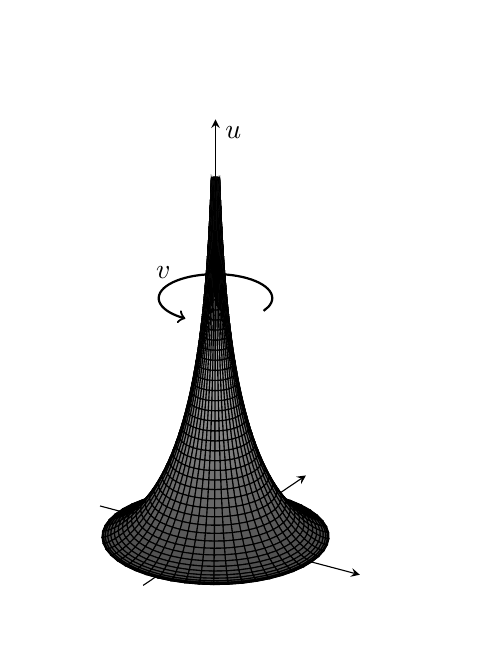
\begin{tikzpicture}[scale=1]

\begin{axis}[%
    width=2.113in,
    height=2.98in,
    at={(1.59in,0.402in)},
    scale only axis,
    plot box ratio=1 1.001 1.502,
    axis lines = middle,
    xmin=-1.2,
    xmax=1.5,
    ticks=none,
    ymin=-1.2,
    ymax=1.5,
    zmin=0,
    zmax=3.5,
    zlabel=\(u\),
    view={32.0545132396862}{25.0188534547135},
    axis background/.style={fill=white},
]
    \addplot3[domain=0:50, ->, thick]
    table[row sep=crcr] {
        0.5  0.0  2\\
        0.49077957849553266  0.09557931435068615  2\\
        0.4793339265183303  0.1422637933155162  2\\
        0.4634583786730109  0.18763350243968704  2\\
        0.44329965318650005  0.23126914512041763  2\\
        0.41904405244592036  0.2727674506052743  2\\
        0.3909157412340149  0.31174490092936674  2\\
        0.35917467504886386  0.3478412753017432  2\\
        0.32411419765389426  0.38072297918456716  2\\
        0.28605833006108483  0.41008612729847793  2\\
        0.24535877600196895  0.4356593520616947  2\\
        0.202391671561197  0.4572063115079062  2\\
        0.15755410901181038  0.4745278735053343  2\\
        0.11126046697815722  0.4874639560909118  2\\
        0.06393858084225311  0.495895006911623  2\\
        0.016025788785827666  0.49974310810034395  2\\
        -0.032035109990356414  0.49897269637516817  2\\
        -0.07979994751668948  0.4935908917072251  2\\
        -0.1268272919547536  0.4836474315195147  2\\
        -0.17268252721065375  0.4692342110248802  2\\
        -0.21694186955877903  0.4504844339512096  2\\
        -0.2591962841552625  0.4275713815026731  2\\
        -0.2990552652456078  0.4007068109339785  2\\
        -0.3361504451306583  0.37013899853765786  2\\
        -0.3701389985376577  0.3361504451306585  2\\
        -0.40070681093397825  0.29905526524560805  2\\
        -0.42757138150267304  0.2591962841552626  2\\
        -0.4504844339512095  0.21694186955877912  2\\
        -0.4692342110248801  0.17268252721065405  2\\
        -0.48364743151951467  0.1268272919547539  2\\
        -0.49359089170722503  0.0797999475166898  2\\
        -0.49897269637516817  0.032035109990356615  2\\
        -0.49974310810034395  -0.01602578878582746  2\\
        -0.4958950069116231  -0.06393858084225292  2\\
        -0.4874639560909118  -0.11126046697815714  2\\
        -0.47452787350533443  -0.1575541090118101  2\\
        -0.45720631150790636  -0.2023916715611967  2\\
        -0.43565935206169476  -0.24535877600196876  2\\
        -0.41008612729847804  -0.28605833006108466  2\\
        -0.3807229791845673  -0.3241141976538941  2\\
        -0.34784127530174325  -0.3591746750488637  2\\
        -0.31174490092936685  -0.39091574123401485  2\\
        -0.2727674506052746  -0.4190440524459202  2\\
        -0.23126914512041766  -0.4432996531865  2\\
        -0.18763350243968727  -0.4634583786730108  2\\
        -0.1422637933155166  -0.4793339265183302  2\\
        -0.0955793143506863  -0.49077957849553266  2\\
        -0.04801151295384122  -0.49768955647459906  2\\
        -9.184850993605148e-17  -0.5  2\\
    } node[pos=0.7, above] {\(v\)};

    \addplot3 [color=mycolor1]
     table[row sep=crcr] {%
    1	0	0\\
    0.996677281521151	0	0.000180848295413094\\
    0.986818657254952	0	0.00143534074664706\\
    0.970744026930539	0	0.00478124968872615\\
    0.948958838413527	0	0.0111306709055737\\
    0.922116636293008	0	0.021251248082997\\
    0.890973941781643	0	0.0357414777260489\\
    0.856342883234364	0	0.0550209162433916\\
    0.819046488706006	0	0.0793340686584179\\
    0.779880351526415	0	0.108765257576638\\
    0.739582863872753	0	0.143261015624456\\
    0.698814736566502	0	0.182656475753605\\
    0.658147333570727	0	0.226702676689377\\
    0.618058560319707	0	0.275092429633295\\
    0.578934654256853	0	0.327483200361739\\
    0.541076158953017	0	0.383516199297968\\
    0.504706515831052	0	0.4428314592909\\
    0.469981979037802	0	0.505079091615864\\
    0.437001869679927	0	0.569927157912677\\
    0.405818482253955	0	0.637066711600307\\
    0.376446209482368	0	0.70621458438625\\
    0.348869650868407	0	0.777114456348854\\
    0.323050615738523	0	0.849536679194129\\
    0.298934030278091	0	0.923277241274682\\
    0.276452819459861	0	0.998156182388777\\
    0.255531868277275	0	1.07401569336226\\
    0.236091180639736	0	1.15071807320667\\
    0.218048355357848	0	1.22814366601495\\
    0.201320491892778	0	1.30618886003915\\
    0.185825627569285	0	1.38476420122183\\
    0.171483795196121	0	1.46379265120814\\
    0.158217777058867	0	1.54320800395986\\
    0.145953618972422	0	1.62295346409914\\
    0.134620956991128	0	1.70298038282444\\
    0.124153199675171	0	1.78324714268591\\
    0.114487600525916	0	1.86371817991473\\
    0.10556524825076	0	1.94436313178065\\
    0.0973309967677409	0	2.02515609616461\\
    0.0897333521584377	0	2.10607499085338\\
    0.0827243299703536	0	2.18710100075792\\
    0.0762592932121512	0	2.26821810216251\\
    0.0702967789469859	0	2.34941265411304\\
    0.0647983194579305	0	2.43067304807599\\
    0.0597282624391434	0	2.51198940799476\\
    0.055053593476748	0	2.59335333380767\\
    0.0507437631581477	0	2.67475768235632\\
    0.0467705204335336	0	2.7561963803967\\
    0.0431077533047957	0	2.8376642651264\\
    0.039731337499592	0	2.91915694826365\\
    0.0366189934736865	0	3.00067070026093\\
    };
     
    \addplot3[%
    surf,
    shader=flat corner, draw=black, z buffer=sort, colormap={mymap}{[1pt] rgb(0pt)=(0.3,0.3,0.3); rgb(255pt)=(1,1,1)}, mesh/rows=50]
    table[row sep=crcr, point meta=\thisrow{c}] {%
    %
    x	y	z	c\\
    1	0	0	0\\
    0.991790013823246	0.127877161684506	0	0\\
    0.967294863039029	0.253654583909507	0	0\\
    0.926916757346022	0.375267004879374	0	0\\
    0.871318704123389	0.490717552003938	0	0\\
    0.801413621867957	0.598110530491216	0	0\\
    0.718349350097728	0.695682550603486	0	0\\
    0.623489801858734	0.78183148246803	0	0\\
    0.518392568310525	0.855142763005346	0	0\\
    0.404783343122394	0.914412623015812	0	0\\
    0.284527586631032	0.958667853036661	0	0\\
    0.15959989503338	0.98718178341445	0	0\\
    0.0320515775716553	0.999486216200688	0	0\\
    -0.0960230259076818	0.995379112949198	0	0\\
    -0.222520933956314	0.974927912181824	0	0\\
    -0.345365054421307	0.93846842204976	0	0\\
    -0.462538290240835	0.886599306373	0	0\\
    -0.57211666012217	0.820172254596956	0	0\\
    -0.672300890261317	0.740277997075315	0	0\\
    -0.761445958369134	0.648228395307789	0	0\\
    -0.838088104891841	0.545534901210549	0	0\\
    -0.900968867902419	0.433883739117558	0	0\\
    -0.949055747010669	0.315108218023621	0	0\\
    -0.981559156991065	0.191158628701373	0	0\\
    -0.997945392750336	0.0640702199807132	0	0\\
    -0.997945392750336	-0.064070219980713	0	0\\
    -0.981559156991065	-0.191158628701372	0	0\\
    -0.949055747010669	-0.315108218023621	0	0\\
    -0.900968867902419	-0.433883739117558	0	0\\
    -0.838088104891841	-0.545534901210548	0	0\\
    -0.761445958369135	-0.648228395307788	0	0\\
    -0.672300890261317	-0.740277997075315	0	0\\
    -0.57211666012217	-0.820172254596956	0	0\\
    -0.462538290240835	-0.886599306373	0	0\\
    -0.345365054421307	-0.938468422049761	0	0\\
    -0.222520933956315	-0.974927912181824	0	0\\
    -0.0960230259076816	-0.995379112949198	0	0\\
    0.0320515775716549	-0.999486216200688	0	0\\
    0.159599895033378	-0.98718178341445	0	0\\
    0.284527586631032	-0.958667853036661	0	0\\
    0.404783343122394	-0.914412623015812	0	0\\
    0.518392568310524	-0.855142763005346	0	0\\
    0.623489801858733	-0.78183148246803	0	0\\
    0.718349350097727	-0.695682550603487	0	0\\
    0.801413621867956	-0.598110530491217	0	0\\
    0.871318704123389	-0.490717552003938	0	0\\
    0.926916757346022	-0.375267004879375	0	0\\
    0.967294863039029	-0.253654583909508	0	0\\
    0.991790013823246	-0.127877161684507	0	0\\
    1	-2.44929359829471e-16	0	0\\
    0.996677281521151	0	0.000180848295413094	0.000180848295413094\\
    0.988494574817178	0.127452261876354	0.000180848295413094	0.000180848295413094\\
    0.964080814523114	0.252811761136307	0.000180848295413094	0.000180848295413094\\
    0.923836873908034	0.374020098267759	0.000180848295413094	0.000180848295413094\\
    0.868423557364232	0.489087035725999	0.000180848295413094	0.000180848295413094\\
    0.798750750017375	0.596123177579159	0.000180848295413094	0.000180848295413094\\
    0.715962477437889	0.693370993337184	0.000180848295413094	0.000180848295413094\\
    0.621418120772724	0.779233676553888	0.000180848295413094	0.000180848295413094\\
    0.516670095744502	0.852301364344654	0.000180848295413094	0.000180848295413094\\
    0.403438362028271	0.911374287296025	0.000180848295413094	0.000180848295413094\\
    0.283582181561191	0.955482469646297	0.000180848295413094	0.000180848295413094\\
    0.15906958951293	0.983901656260716	0.000180848295413094	0.000180848295413094\\
    0.0319450792025817	0.996165204880763	0.000180848295413094	0.000180848295413094\\
    -0.0957039684251033	0.992071748377142	0.000180848295413094	0.000180848295413094\\
    -0.221781559537127	0.971688501192472	0.000180848295413094	0.000180848295413094\\
    -0.344217503573033	0.935350155682	0.000180848295413094	0.000180848295413094\\
    -0.461001405716677	0.88365338647438	0.000180848295413094	0.000180848295413094\\
    -0.570215677523525	0.817447053090767	0.000180848295413094	0.000180848295413094\\
    -0.670067023669899	0.737818261694948	0.000180848295413094	0.000180848295413094\\
    -0.758915887812616	0.646074514840185	0.000180848295413094	0.000180848295413094\\
    -0.835303374058813	0.543722242313439	0.000180848295413094	0.000180848295413094\\
    -0.897975201996172	0.43244206559992	0.000180848295413094	0.000180848295413094\\
    -0.945902301942619	0.314061202124757	0.000180848295413094	0.000180848295413094\\
    -0.978297712242048	0.190523462393395	0.000180848295413094	0.000180848295413094\\
    -0.994629501152963	0.0638573326768394	0.000180848295413094	0.000180848295413094\\
    -0.994629501152963	-0.0638573326768392	0.000180848295413094	0.000180848295413094\\
    -0.978297712242048	-0.190523462393395	0.000180848295413094	0.000180848295413094\\
    -0.945902301942619	-0.314061202124756	0.000180848295413094	0.000180848295413094\\
    -0.897975201996172	-0.43244206559992	0.000180848295413094	0.000180848295413094\\
    -0.835303374058813	-0.543722242313439	0.000180848295413094	0.000180848295413094\\
    -0.758915887812617	-0.646074514840185	0.000180848295413094	0.000180848295413094\\
    -0.670067023669899	-0.737818261694948	0.000180848295413094	0.000180848295413094\\
    -0.570215677523525	-0.817447053090767	0.000180848295413094	0.000180848295413094\\
    -0.461001405716677	-0.88365338647438	0.000180848295413094	0.000180848295413094\\
    -0.344217503573033	-0.935350155682	0.000180848295413094	0.000180848295413094\\
    -0.221781559537127	-0.971688501192472	0.000180848295413094	0.000180848295413094\\
    -0.0957039684251031	-0.992071748377142	0.000180848295413094	0.000180848295413094\\
    0.0319450792025813	-0.996165204880763	0.000180848295413094	0.000180848295413094\\
    0.159069589512929	-0.983901656260716	0.000180848295413094	0.000180848295413094\\
    0.283582181561191	-0.955482469646298	0.000180848295413094	0.000180848295413094\\
    0.403438362028271	-0.911374287296025	0.000180848295413094	0.000180848295413094\\
    0.516670095744501	-0.852301364344655	0.000180848295413094	0.000180848295413094\\
    0.621418120772724	-0.779233676553888	0.000180848295413094	0.000180848295413094\\
    0.715962477437888	-0.693370993337184	0.000180848295413094	0.000180848295413094\\
    0.798750750017374	-0.59612317757916	0.000180848295413094	0.000180848295413094\\
    0.868423557364232	-0.489087035725999	0.000180848295413094	0.000180848295413094\\
    0.923836873908033	-0.37402009826776	0.000180848295413094	0.000180848295413094\\
    0.964080814523114	-0.252811761136307	0.000180848295413094	0.000180848295413094\\
    0.988494574817178	-0.127452261876355	0.000180848295413094	0.000180848295413094\\
    0.996677281521151	-2.44115528519553e-16	0.000180848295413094	0.000180848295413094\\
    0.986818657254952	0	0.00143534074664706	0.00143534074664706\\
    0.978716889719926	0.126191568987079	0.00143534074664706	0.00143534074664706\\
    0.954544617913788	0.250311075900144	0.00143534074664706	0.00143534074664706\\
    0.914698749871315	0.370320481867152	0.00143534074664706	0.00143534074664706\\
    0.859833553644168	0.484249235759963	0.00143534074664706	0.00143534074664706\\
    0.790849914237565	0.590226630589389	0.00143534074664706	0.00143534074664706\\
    0.708880541103407	0.686512520462233	0.00143534074664706	0.00143534074664706\\
    0.615271369082392	0.77152589372875	0.00143534074664706	0.00143534074664706\\
    0.511559458191139	0.843870833150225	0.00143534074664706	0.00143534074664706\\
    0.399447755139211	0.902359436821443	0.00143534074664706	0.00143534074664706\\
    0.280777130991228	0.946031323487125	0.00143534074664706	0.00143534074664706\\
    0.157496154114871	0.974169401975597	0.00143534074664706	0.00143534074664706\\
    0.0316290947421639	0.986311645815996	0.00143534074664706	0.00143534074664706\\
    -0.094757313491776	0.982258679700153	0.00143534074664706	0.00143534074664706\\
    -0.219587809257888	0.962077053219641	0.00143534074664706	0.00143534074664706\\
    -0.340812679266818	0.926098148123318	0.00143534074664706	0.00143534074664706\\
    -0.456441414504462	0.874912737038176	0.00143534074664706	0.00143534074664706\\
    -0.564575394334947	0.809361282999135	0.00143534074664706	0.00143534074664706\\
    -0.663439061798982	0.730520139069248	0.00143534074664706	0.00143534074664706\\
    -0.751409078210039	0.639683874652164	0.00143534074664706	0.00143534074664706\\
    -0.827040978330714	0.538344018698307	0.00143534074664706	0.00143534074664706\\
    -0.88909288845198	0.428164568840747	0.00143534074664706	0.00143534074664706\\
    -0.936545917925164	0.310954668600071	0.00143534074664706	0.00143534074664706\\
    -0.968620889318226	0.188638901297786	0.00143534074664706	0.00143534074664706\\
    -0.984791132487653	0.0632256884513968	0.00143534074664706	0.00143534074664706\\
    -0.984791132487653	-0.0632256884513966	0.00143534074664706	0.00143534074664706\\
    -0.968620889318226	-0.188638901297786	0.00143534074664706	0.00143534074664706\\
    -0.936545917925164	-0.31095466860007	0.00143534074664706	0.00143534074664706\\
    -0.88909288845198	-0.428164568840747	0.00143534074664706	0.00143534074664706\\
    -0.827040978330714	-0.538344018698307	0.00143534074664706	0.00143534074664706\\
    -0.75140907821004	-0.639683874652164	0.00143534074664706	0.00143534074664706\\
    -0.663439061798982	-0.730520139069248	0.00143534074664706	0.00143534074664706\\
    -0.564575394334948	-0.809361282999135	0.00143534074664706	0.00143534074664706\\
    -0.456441414504462	-0.874912737038176	0.00143534074664706	0.00143534074664706\\
    -0.340812679266818	-0.926098148123318	0.00143534074664706	0.00143534074664706\\
    -0.219587809257888	-0.962077053219641	0.00143534074664706	0.00143534074664706\\
    -0.0947573134917758	-0.982258679700153	0.00143534074664706	0.00143534074664706\\
    0.0316290947421634	-0.986311645815996	0.00143534074664706	0.00143534074664706\\
    0.15749615411487	-0.974169401975597	0.00143534074664706	0.00143534074664706\\
    0.280777130991227	-0.946031323487125	0.00143534074664706	0.00143534074664706\\
    0.399447755139211	-0.902359436821443	0.00143534074664706	0.00143534074664706\\
    0.511559458191138	-0.843870833150226	0.00143534074664706	0.00143534074664706\\
    0.615271369082391	-0.77152589372875	0.00143534074664706	0.00143534074664706\\
    0.708880541103407	-0.686512520462233	0.00143534074664706	0.00143534074664706\\
    0.790849914237564	-0.59022663058939	0.00143534074664706	0.00143534074664706\\
    0.859833553644168	-0.484249235759963	0.00143534074664706	0.00143534074664706\\
    0.914698749871315	-0.370320481867152	0.00143534074664706	0.00143534074664706\\
    0.954544617913788	-0.250311075900144	0.00143534074664706	0.00143534074664706\\
    0.978716889719926	-0.126191568987079	0.00143534074664706	0.00143534074664706\\
    0.986818657254952	-2.41700861989233e-16	0.00143534074664706	0.00143534074664706\\
    0.970744026930539	0	0.00478124968872615	0.00478124968872615\\
    0.962774231888273	0.124135990886065	0.00478124968872615	0.00478124968872615\\
    0.938995710575732	0.246233672233705	0.00478124968872615	0.00478124968872615\\
    0.899798905655474	0.364288203490766	0.00478124968872615	0.00478124968872615\\
    0.845827427580638	0.476361132517799	0.00478124968872615	0.00478124968872615\\
    0.777967486529088	0.580612224918604	0.00478124968872615	0.00478124968872615\\
    0.697333340856804	0.675329680638137	0.00478124968872615	0.00478124968872615\\
    0.605249001006471	0.758958241672088	0.00478124968872615	0.00478124968872615\\
    0.503226489292624	0.830124729360317	0.00478124968872615	0.00478124968872615\\
    0.392941012537039	0.887660591942487	0.00478124968872615	0.00478124968872615\\
    0.276203455219036	0.930621092145662	0.00478124968872615	0.00478124968872615\\
    0.154930644802394	0.958300819744214	0.00478124968872615	0.00478124968872615\\
    0.0311138774813852	0.970245274376223	0.00478124968872615	0.00478124968872615\\
    -0.0932137788476785	0.966258328426852	0.00478124968872615	0.00478124968872615\\
    -0.216010867505097	0.946405447438366	0.00478124968872615	0.00478124968872615\\
    -0.335261063690025	0.911012615167733	0.00478124968872615	0.00478124968872615\\
    -0.449006282477955	0.860660980942349	0.00478124968872615	0.00478124968872615\\
    -0.555378830521046	0.796177317204148	0.00478124968872615	0.00478124968872615\\
    -0.652632073521257	0.718620443928966	0.00478124968872615	0.00478124968872615\\
    -0.739169115917237	0.629263842831804	0.00478124968872615	0.00478124968872615\\
    -0.813569021865289	0.529574746832282	0.00478124968872615	0.00478124968872615\\
    -0.874610146966643	0.421190048130658	0.00478124968872615	0.00478124968872615\\
    -0.921290197634707	0.305889420483156	0.00478124968872615	0.00478124968872615\\
    -0.952842688728052	0.18556609700809	0.00478124968872615	0.00478124968872615\\
    -0.96874952921524	0.062195783350403	0.00478124968872615	0.00478124968872615\\
    -0.96874952921524	-0.0621957833504028	0.00478124968872615	0.00478124968872615\\
    -0.952842688728052	-0.18556609700809	0.00478124968872615	0.00478124968872615\\
    -0.921290197634707	-0.305889420483156	0.00478124968872615	0.00478124968872615\\
    -0.874610146966643	-0.421190048130658	0.00478124968872615	0.00478124968872615\\
    -0.813569021865289	-0.529574746832282	0.00478124968872615	0.00478124968872615\\
    -0.739169115917237	-0.629263842831804	0.00478124968872615	0.00478124968872615\\
    -0.652632073521257	-0.718620443928965	0.00478124968872615	0.00478124968872615\\
    -0.555378830521046	-0.796177317204148	0.00478124968872615	0.00478124968872615\\
    -0.449006282477955	-0.860660980942349	0.00478124968872615	0.00478124968872615\\
    -0.335261063690025	-0.911012615167733	0.00478124968872615	0.00478124968872615\\
    -0.216010867505097	-0.946405447438366	0.00478124968872615	0.00478124968872615\\
    -0.0932137788476783	-0.966258328426852	0.00478124968872615	0.00478124968872615\\
    0.0311138774813848	-0.970245274376223	0.00478124968872615	0.00478124968872615\\
    0.154930644802393	-0.958300819744215	0.00478124968872615	0.00478124968872615\\
    0.276203455219036	-0.930621092145662	0.00478124968872615	0.00478124968872615\\
    0.392941012537039	-0.887660591942487	0.00478124968872615	0.00478124968872615\\
    0.503226489292623	-0.830124729360317	0.00478124968872615	0.00478124968872615\\
    0.605249001006471	-0.758958241672088	0.00478124968872615	0.00478124968872615\\
    0.697333340856803	-0.675329680638137	0.00478124968872615	0.00478124968872615\\
    0.777967486529088	-0.580612224918605	0.00478124968872615	0.00478124968872615\\
    0.845827427580638	-0.476361132517799	0.00478124968872615	0.00478124968872615\\
    0.899798905655474	-0.364288203490766	0.00478124968872615	0.00478124968872615\\
    0.938995710575732	-0.246233672233706	0.00478124968872615	0.00478124968872615\\
    0.962774231888273	-0.124135990886066	0.00478124968872615	0.00478124968872615\\
    0.970744026930539	-2.37763713074379e-16	0.00478124968872615	0.00478124968872615\\
    0.948958838413527	0	0.0111306709055737	0.0111306709055737\\
    0.941167899467844	0.121350162811748	0.0111306709055737	0.0111306709055737\\
    0.917923009632889	0.240707759305033	0.0111306709055737	0.0111306709055737\\
    0.879605849357114	0.356112941045254	0.0111306709055737	0.0111306709055737\\
    0.826845585352911	0.465670758138787	0.0111306709055737	0.0111306709055737\\
    0.760508539696594	0.567582274257843	0.0111306709055737	0.0111306709055737\\
    0.681683964843852	0.660174105125244	0.0111306709055737	0.0111306709055737\\
    0.591666158134544	0.741925895437988	0.0111306709055737	0.0111306709055737\\
    0.491933209466161	0.811495283059287	0.0111306709055737	0.0111306709055737\\
    0.384122731098571	0.867739940567752	0.0111306709055737	0.0111306709055737\\
    0.270004968105989	0.90973633224206	0.0111306709055737	0.0111306709055737\\
    0.151453731001797	0.936794878491971	0.0111306709055737	0.0111306709055737\\
    0.0304156278217191	0.948471278736136	0.0111306709055737	0.0111306709055737\\
    -0.0911218991263057	0.944573806805358	0.0111306709055737	0.0111306709055737\\
    -0.211163207009877	0.925166459080989	0.0111306709055737	0.0111306709055737\\
    -0.327737220872269	0.890567903676116	0.0111306709055737	0.0111306709055737\\
    -0.438929798628722	0.841346247913961	0.0111306709055737	0.0111306709055737\\
    -0.542915161226561	0.778309710021331	0.0111306709055737	0.0111306709055737\\
    -0.637985871886759	0.702493348207684	0.0111306709055737	0.0111306709055737\\
    -0.722580872168649	0.615142065037944	0.0111306709055737	0.0111306709055737\\
    -0.795311114506355	0.517690166166801	0.0111306709055737	0.0111306709055737\\
    -0.85498237033143	0.411737809079516	0.0111306709055737	0.0111306709055737\\
    -0.900614839272926	0.299024728550252	0.0111306709055737	0.0111306709055737\\
    -0.931459237452402	0.181401670245177	0.0111306709055737	0.0111306709055737\\
    -0.94700910070449	0.0608000015297968	0.0111306709055737	0.0111306709055737\\
    -0.94700910070449	-0.0608000015297966	0.0111306709055737	0.0111306709055737\\
    -0.931459237452402	-0.181401670245177	0.0111306709055737	0.0111306709055737\\
    -0.900614839272927	-0.299024728550251	0.0111306709055737	0.0111306709055737\\
    -0.85498237033143	-0.411737809079516	0.0111306709055737	0.0111306709055737\\
    -0.795311114506355	-0.5176901661668	0.0111306709055737	0.0111306709055737\\
    -0.722580872168649	-0.615142065037943	0.0111306709055737	0.0111306709055737\\
    -0.63798587188676	-0.702493348207684	0.0111306709055737	0.0111306709055737\\
    -0.542915161226561	-0.778309710021331	0.0111306709055737	0.0111306709055737\\
    -0.438929798628722	-0.841346247913961	0.0111306709055737	0.0111306709055737\\
    -0.327737220872268	-0.890567903676117	0.0111306709055737	0.0111306709055737\\
    -0.211163207009878	-0.925166459080989	0.0111306709055737	0.0111306709055737\\
    -0.0911218991263055	-0.944573806805358	0.0111306709055737	0.0111306709055737\\
    0.0304156278217187	-0.948471278736136	0.0111306709055737	0.0111306709055737\\
    0.151453731001796	-0.936794878491971	0.0111306709055737	0.0111306709055737\\
    0.270004968105988	-0.90973633224206	0.0111306709055737	0.0111306709055737\\
    0.384122731098571	-0.867739940567752	0.0111306709055737	0.0111306709055737\\
    0.49193320946616	-0.811495283059288	0.0111306709055737	0.0111306709055737\\
    0.591666158134544	-0.741925895437988	0.0111306709055737	0.0111306709055737\\
    0.681683964843851	-0.660174105125245	0.0111306709055737	0.0111306709055737\\
    0.760508539696593	-0.567582274257844	0.0111306709055737	0.0111306709055737\\
    0.826845585352911	-0.465670758138787	0.0111306709055737	0.0111306709055737\\
    0.879605849357114	-0.356112941045255	0.0111306709055737	0.0111306709055737\\
    0.917923009632889	-0.240707759305033	0.0111306709055737	0.0111306709055737\\
    0.941167899467844	-0.121350162811748	0.0111306709055737	0.0111306709055737\\
    0.948958838413527	-2.32427880797143e-16	0.0111306709055737	0.0111306709055737\\
    0.922116636293008	0	0.021251248082997	0.021251248082997\\
    0.914546071455688	0.117917658191214	0.021251248082997	0.021251248082997\\
    0.891958685409056	0.233899111694937	0.021251248082997	0.021251248082997\\
    0.854725362407536	0.34603994825112	0.021251248082997	0.021251248082997\\
    0.803457472585443	0.45249881842381	0.021251248082997	0.021251248082997\\
    0.738996833276277	0.551527670507987	0.021251248082997	0.021251248082997\\
    0.662401886395385	0.641500453490227	0.021251248082997	0.021251248082997\\
    0.57493031885297	0.720939816761396	0.021251248082997	0.021251248082997\\
    0.478018411369795	0.788541368172799	0.021251248082997	0.021251248082997\\
    0.37325745478746	0.843195092119208	0.021251248082997	0.021251248082997\\
    0.262367621116775	0.884003575964405	0.021251248082997	0.021251248082997\\
    0.147169718360897	0.910296745531866	0.021251248082997	0.021251248082997\\
    0.0295552928982592	0.921642867704205	0.021251248082997	0.021251248082997\\
    -0.0885444296566679	0.917855639469033	0.021251248082997	0.021251248082997\\
    -0.205190255124575	0.898997247009268	0.021251248082997	0.021251248082997\\
    -0.318466862276128	0.865377344607732	0.021251248082997	0.021251248082997\\
    -0.426514252353598	0.817547970132385	0.021251248082997	0.021251248082997\\
    -0.527558290199045	0.756294480589798	0.021251248082997	0.021251248082997\\
    -0.61993983550456	0.682622656584815	0.021251248082997	0.021251248082997\\
    -0.702141985850252	0.597742187430833	0.021251248082997	0.021251248082997\\
    -0.772814984200046	0.50304680808471	0.021251248082997	0.021251248082997\\
    -0.830798381874898	0.400091414057316	0.021251248082997	0.021251248082997\\
    -0.875140093088026	0.290566530072225	0.021251248082997	0.021251248082997\\
    -0.905112028167202	0.176270551696494	0.021251248082997	0.021251248082997\\
    -0.920222048767045	0.0590802157351684	0.021251248082997	0.021251248082997\\
    -0.920222048767045	-0.0590802157351681	0.021251248082997	0.021251248082997\\
    -0.905112028167202	-0.176270551696493	0.021251248082997	0.021251248082997\\
    -0.875140093088026	-0.290566530072225	0.021251248082997	0.021251248082997\\
    -0.830798381874898	-0.400091414057316	0.021251248082997	0.021251248082997\\
    -0.772814984200046	-0.503046808084709	0.021251248082997	0.021251248082997\\
    -0.702141985850252	-0.597742187430832	0.021251248082997	0.021251248082997\\
    -0.61993983550456	-0.682622656584815	0.021251248082997	0.021251248082997\\
    -0.527558290199046	-0.756294480589797	0.021251248082997	0.021251248082997\\
    -0.426514252353598	-0.817547970132385	0.021251248082997	0.021251248082997\\
    -0.318466862276128	-0.865377344607732	0.021251248082997	0.021251248082997\\
    -0.205190255124575	-0.898997247009268	0.021251248082997	0.021251248082997\\
    -0.0885444296566677	-0.917855639469033	0.021251248082997	0.021251248082997\\
    0.0295552928982588	-0.921642867704205	0.021251248082997	0.021251248082997\\
    0.147169718360896	-0.910296745531866	0.021251248082997	0.021251248082997\\
    0.262367621116775	-0.884003575964405	0.021251248082997	0.021251248082997\\
    0.37325745478746	-0.843195092119208	0.021251248082997	0.021251248082997\\
    0.478018411369794	-0.788541368172799	0.021251248082997	0.021251248082997\\
    0.574930318852969	-0.720939816761396	0.021251248082997	0.021251248082997\\
    0.662401886395385	-0.641500453490228	0.021251248082997	0.021251248082997\\
    0.738996833276276	-0.551527670507988	0.021251248082997	0.021251248082997\\
    0.803457472585443	-0.45249881842381	0.021251248082997	0.021251248082997\\
    0.854725362407536	-0.346039948251121	0.021251248082997	0.021251248082997\\
    0.891958685409056	-0.233899111694938	0.021251248082997	0.021251248082997\\
    0.914546071455688	-0.117917658191214	0.021251248082997	0.021251248082997\\
    0.922116636293008	-2.25853437415351e-16	0.021251248082997	0.021251248082997\\
    0.890973941781643	0	0.0357414777260489	0.0357414777260489\\
    0.883659058035767	0.113935218809893	0.0357414777260489	0.0357414777260489\\
    0.861834516987018	0.225999624476836	0.0357414777260489	0.0357414777260489\\
    0.825858676996043	0.334353122557967	0.0357414777260489	0.0357414777260489\\
    0.776322260360889	0.437216551610387	0.0357414777260489	0.0357414777260489\\
    0.714038653673196	0.532900896972868	0.0357414777260489	0.0357414777260489\\
    0.640030552032854	0.619835024339895	0.0357414777260489	0.0357414777260489\\
    0.555513166422731	0.696591477743526	0.0357414777260489	0.0357414777260489\\
    0.461874269977938	0.761909918340918	0.0357414777260489	0.0357414777260489\\
    0.36065141078931	0.81471781914329	0.0357414777260489	0.0357414777260489\\
    0.253506665406269	0.854148075879418	0.0357414777260489	0.0357414777260489\\
    0.142199347585827	0.879553244823804	0.0357414777260489	0.0357414777260489\\
    0.0285571204093378	0.890516173804746	0.0357414777260489	0.0357414777260489\\
    -0.085554013894768	0.886856851831462	0.0357414777260489	0.0357414777260489\\
    -0.19826035365599	0.868635364869586	0.0357414777260489	0.0357414777260489\\
    -0.307711263891384	0.836150909231273	0.0357414777260489	0.0357414777260489\\
    -0.412109563680818	0.789936878780022	0.0357414777260489	0.0357414777260489\\
    -0.509741035827998	0.730752106618187	0.0357414777260489	0.0357414777260489\\
    -0.599002574259433	0.659568405068413	0.0357414777260489	0.0357414777260489\\
    -0.678428506981848	0.577554608542169	0.0357414777260489	0.0357414777260489\\
    -0.74671466237579	0.486057381311022	0.0357414777260489	0.0357414777260489\\
    -0.802739783657562	0.386579105316529	0.0357414777260489	0.0357414777260489\\
    -0.845583939884617	0.280753211100295	0.0357414777260489	0.0357414777260489\\
    -0.874543631196196	0.170317356919635	0.0357414777260489	0.0357414777260489\\
    -0.889143340261597	0.057084896447033	0.0357414777260489	0.0357414777260489\\
    -0.889143340261597	-0.0570848964470328	0.0357414777260489	0.0357414777260489\\
    -0.874543631196196	-0.170317356919635	0.0357414777260489	0.0357414777260489\\
    -0.845583939884617	-0.280753211100294	0.0357414777260489	0.0357414777260489\\
    -0.802739783657562	-0.386579105316529	0.0357414777260489	0.0357414777260489\\
    -0.74671466237579	-0.486057381311021	0.0357414777260489	0.0357414777260489\\
    -0.678428506981848	-0.577554608542169	0.0357414777260489	0.0357414777260489\\
    -0.599002574259433	-0.659568405068413	0.0357414777260489	0.0357414777260489\\
    -0.509741035827998	-0.730752106618187	0.0357414777260489	0.0357414777260489\\
    -0.412109563680819	-0.789936878780022	0.0357414777260489	0.0357414777260489\\
    -0.307711263891384	-0.836150909231273	0.0357414777260489	0.0357414777260489\\
    -0.19826035365599	-0.868635364869586	0.0357414777260489	0.0357414777260489\\
    -0.0855540138947678	-0.886856851831462	0.0357414777260489	0.0357414777260489\\
    0.0285571204093374	-0.890516173804746	0.0357414777260489	0.0357414777260489\\
    0.142199347585826	-0.879553244823805	0.0357414777260489	0.0357414777260489\\
    0.253506665406268	-0.854148075879418	0.0357414777260489	0.0357414777260489\\
    0.36065141078931	-0.81471781914329	0.0357414777260489	0.0357414777260489\\
    0.461874269977937	-0.761909918340919	0.0357414777260489	0.0357414777260489\\
    0.555513166422731	-0.696591477743526	0.0357414777260489	0.0357414777260489\\
    0.640030552032853	-0.619835024339896	0.0357414777260489	0.0357414777260489\\
    0.714038653673196	-0.532900896972869	0.0357414777260489	0.0357414777260489\\
    0.776322260360889	-0.437216551610387	0.0357414777260489	0.0357414777260489\\
    0.825858676996043	-0.334353122557967	0.0357414777260489	0.0357414777260489\\
    0.861834516987018	-0.225999624476836	0.0357414777260489	0.0357414777260489\\
    0.883659058035767	-0.113935218809893	0.0357414777260489	0.0357414777260489\\
    0.890973941781643	-2.18225677185318e-16	0.0357414777260489	0.0357414777260489\\
    0.856342883234364	0	0.0550209162433916	0.0550209162433916\\
    0.849312320000449	0.109506697336737	0.0550209162433916	0.0550209162433916\\
    0.828336071952632	0.217215297730681	0.0550209162433916	0.0550209162433916\\
    0.79375856850394	0.321357228941128	0.0550209162433916	0.0550209162433916\\
    0.746147571305053	0.420222483336761	0.0550209162433916	0.0550209162433916\\
    0.686284851613701	0.512187696173683	0.0550209162433916	0.0550209162433916\\
    0.61515335363222	0.595742801199626	0.0550209162433916	0.0550209162433916\\
    0.533921054590931	0.66951582590007	0.0550209162433916	0.0550209162433916\\
    0.443921786594302	0.732295419248999	0.0550209162433916	0.0550209162433916\\
    0.346633335134676	0.783050742059259	0.0550209162433916	0.0550209162433916\\
    0.243653173895334	0.820948393333512	0.0550209162433916	0.0550209162433916\\
    0.136672234276786	0.845366094685572	0.0550209162433916	0.0550209162433916\\
    0.0274471403499212	0.855902908134302	0.0550209162433916	0.0550209162433916\\
    -0.0822286348626723	0.85238581949418	0.0550209162433916	0.0550209162433916\\
    -0.190554218164154	0.834872579263442	0.0550209162433916	0.0550209162433916\\
    -0.295750906471536	0.803650754362496	0.0550209162433916	0.0550209162433916\\
    -0.39609137307113	0.759233006293043	0.0550209162433916	0.0550209162433916\\
    -0.489928030275434	0.702348673250386	0.0550209162433916	0.0550209162433916\\
    -0.575720082767406	0.633931794410436	0.0550209162433916	0.0550209162433916\\
    -0.652058827416978	0.555105773032257	0.0550209162433916	0.0550209162433916\\
    -0.717690784147503	0.467164930207615	0.0550209162433916	0.0550209162433916\\
    -0.771538278043959	0.371553252144437	0.0550209162433916	0.0550209162433916\\
    -0.812717134745259	0.269840679953191	0.0550209162433916	0.0550209162433916\\
    -0.840551198562821	0.163697331257261	0.0550209162433916	0.0550209162433916\\
    -0.854583434938273	0.054866076907744	0.0550209162433916	0.0550209162433916\\
    -0.854583434938273	-0.0548660769077437	0.0550209162433916	0.0550209162433916\\
    -0.840551198562821	-0.16369733125726	0.0550209162433916	0.0550209162433916\\
    -0.81271713474526	-0.26984067995319	0.0550209162433916	0.0550209162433916\\
    -0.771538278043959	-0.371553252144436	0.0550209162433916	0.0550209162433916\\
    -0.717690784147503	-0.467164930207615	0.0550209162433916	0.0550209162433916\\
    -0.652058827416979	-0.555105773032257	0.0550209162433916	0.0550209162433916\\
    -0.575720082767406	-0.633931794410436	0.0550209162433916	0.0550209162433916\\
    -0.489928030275434	-0.702348673250386	0.0550209162433916	0.0550209162433916\\
    -0.39609137307113	-0.759233006293042	0.0550209162433916	0.0550209162433916\\
    -0.295750906471536	-0.803650754362496	0.0550209162433916	0.0550209162433916\\
    -0.190554218164154	-0.834872579263442	0.0550209162433916	0.0550209162433916\\
    -0.0822286348626721	-0.85238581949418	0.0550209162433916	0.0550209162433916\\
    0.0274471403499208	-0.855902908134302	0.0550209162433916	0.0550209162433916\\
    0.136672234276785	-0.845366094685572	0.0550209162433916	0.0550209162433916\\
    0.243653173895333	-0.820948393333512	0.0550209162433916	0.0550209162433916\\
    0.346633335134676	-0.783050742059259	0.0550209162433916	0.0550209162433916\\
    0.443921786594302	-0.732295419248999	0.0550209162433916	0.0550209162433916\\
    0.53392105459093	-0.66951582590007	0.0550209162433916	0.0550209162433916\\
    0.615153353632219	-0.595742801199627	0.0550209162433916	0.0550209162433916\\
    0.6862848516137	-0.512187696173684	0.0550209162433916	0.0550209162433916\\
    0.746147571305053	-0.420222483336761	0.0550209162433916	0.0550209162433916\\
    0.79375856850394	-0.321357228941128	0.0550209162433916	0.0550209162433916\\
    0.828336071952632	-0.217215297730681	0.0550209162433916	0.0550209162433916\\
    0.849312320000449	-0.109506697336737	0.0550209162433916	0.0550209162433916\\
    0.856342883234364	-2.09743514185116e-16	0.0550209162433916	0.0550209162433916\\
    0.819046488706006	0	0.0793340686584179	0.0793340686584179\\
    0.812322128355611	0.104737340263385	0.0793340686584179	0.0793340686584179\\
    0.792259461115474	0.207754896295265	0.0793340686584179	0.0793340686584179\\
    0.759187915427016	0.307361122673671	0.0793340686584179	0.0793340686584179\\
    0.713650525156129	0.401920487915232	0.0793340686584179	0.0793340686584179\\
    0.656395012992113	0.489880329856917	0.0793340686584179	0.0793340686584179\\
    0.588361512861785	0.569796350325824	0.0793340686584179	0.0793340686584179\\
    0.510667132956399	0.640356330475251	0.0793340686584179	0.0793340686584179\\
    0.424587612846024	0.700401677381881	0.0793340686584179	0.0793340686584179\\
    0.331536375871075	0.74894644810955	0.0793340686584179	0.0793340686584179\\
    0.233041320770141	0.785193538865002	0.0793340686584179	0.0793340686584179\\
    0.130719733624937	0.808547773420138	0.0793340686584179	0.0793340686584179\\
    0.0262517320675525	0.818625675889225	0.0793340686584179	0.0793340686584179\\
    -0.0786473222046126	0.81526176739234	0.0793340686584179	0.0793340686584179\\
    -0.1822549896205	0.798511283214	0.0793340686584179	0.0793340686584179\\
    -0.282870035145531	0.768649265841322	0.0793340686584179	0.0793340686584179\\
    -0.378840362513836	0.726166048773986	0.0793340686584179	0.0793340686584179\\
    -0.468590141603271	0.671759205261725	0.0793340686584179	0.0793340686584179\\
    -0.550645683522453	0.606322094170852	0.0793340686584179	0.0793340686584179\\
    -0.623659638541619	0.530929191056373	0.0793340686584179	0.0793340686584179\\
    -0.686433119537933	0.446818445303078	0.0793340686584179	0.0793340686584179\\
    -0.737935387688902	0.355370953030869	0.0793340686584179	0.0793340686584179\\
    -0.777320777175344	0.258088279534654	0.0793340686584179	0.0793340686584179\\
    -0.803942580990759	0.156567803623714	0.0793340686584179	0.0793340686584179\\
    -0.817363669852499	0.0524764887058246	0.0793340686584179	0.0793340686584179\\
    -0.817363669852499	-0.0524764887058244	0.0793340686584179	0.0793340686584179\\
    -0.803942580990759	-0.156567803623714	0.0793340686584179	0.0793340686584179\\
    -0.777320777175344	-0.258088279534653	0.0793340686584179	0.0793340686584179\\
    -0.737935387688902	-0.355370953030869	0.0793340686584179	0.0793340686584179\\
    -0.686433119537933	-0.446818445303078	0.0793340686584179	0.0793340686584179\\
    -0.623659638541619	-0.530929191056373	0.0793340686584179	0.0793340686584179\\
    -0.550645683522454	-0.606322094170852	0.0793340686584179	0.0793340686584179\\
    -0.468590141603271	-0.671759205261725	0.0793340686584179	0.0793340686584179\\
    -0.378840362513836	-0.726166048773986	0.0793340686584179	0.0793340686584179\\
    -0.28287003514553	-0.768649265841323	0.0793340686584179	0.0793340686584179\\
    -0.182254989620501	-0.798511283214	0.0793340686584179	0.0793340686584179\\
    -0.0786473222046124	-0.81526176739234	0.0793340686584179	0.0793340686584179\\
    0.0262517320675521	-0.818625675889225	0.0793340686584179	0.0793340686584179\\
    0.130719733624936	-0.808547773420139	0.0793340686584179	0.0793340686584179\\
    0.233041320770141	-0.785193538865002	0.0793340686584179	0.0793340686584179\\
    0.331536375871075	-0.74894644810955	0.0793340686584179	0.0793340686584179\\
    0.424587612846023	-0.700401677381881	0.0793340686584179	0.0793340686584179\\
    0.510667132956399	-0.640356330475251	0.0793340686584179	0.0793340686584179\\
    0.588361512861785	-0.569796350325824	0.0793340686584179	0.0793340686584179\\
    0.656395012992112	-0.489880329856918	0.0793340686584179	0.0793340686584179\\
    0.713650525156129	-0.401920487915232	0.0793340686584179	0.0793340686584179\\
    0.759187915427016	-0.307361122673671	0.0793340686584179	0.0793340686584179\\
    0.792259461115474	-0.207754896295265	0.0793340686584179	0.0793340686584179\\
    0.812322128355611	-0.104737340263385	0.0793340686584179	0.0793340686584179\\
    0.819046488706006	-2.00608532149338e-16	0.0793340686584179	0.0793340686584179\\
    0.779880351526415	0	0.108765257576638	0.108765257576638\\
    0.773477544620862	0.0997288858067128	0.108765257576638	0.108765257576638\\
    0.754374257816574	0.197820226065633	0.108765257576638	0.108765257576638\\
    0.722884166554741	0.292663363681591	0.108765257576638	0.108765257576638\\
    0.67952433726329	0.382700976957013	0.108765257576638	0.108765257576638\\
    0.62500673714044	0.46645465077114	0.108765257576638	0.108765257576638\\
    0.560226543672988	0.54254915211544	0.108765257576638	0.108765257576638\\
    0.486247445846724	0.609735011381586	0.108765257576638	0.108765257576638\\
    0.404284178402694	0.666909038617879	0.108765257576638	0.108765257576638\\
    0.31568257592633	0.713132437877763	0.108765257576638	0.108765257576638\\
    0.221897474280772	0.747646222223305	0.108765257576638	0.108765257576638\\
    0.124468822242211	0.769883676269735	0.108765257576638	0.108765257576638\\
    0.0249963955835587	0.779479661636399	0.108765257576638	0.108765257576638\\
    -0.0748864711995129	0.776276612508872	0.108765257576638	0.108765257576638\\
    -0.173539704195837	0.760327122865275	0.108765257576638	0.108765257576638\\
    -0.269343420047029	0.731893082884608	0.108765257576638	0.108765257576638\\
    -0.36072452438745	0.691441378717251	0.108765257576638	0.108765257576638\\
    -0.446182542010197	0.639636226227287	0.108765257576638	0.108765257576638\\
    -0.524314254628518	0.577328264586368	0.108765257576638	0.108765257576638\\
    -0.593836741681289	0.505540588802042	0.108765257576638	0.108765257576638\\
    -0.653608445853156	0.425451950526011	0.108765257576638	0.108765257576638\\
    -0.702647917414095	0.338377402984597	0.108765257576638	0.108765257576638\\
    -0.740149929596845	0.245746707841124	0.108765257576638	0.108765257576638\\
    -0.765498700398164	0.149080858548934	0.108765257576638	0.108765257576638\\
    -0.778278003702299	0.0499671056809334	0.108765257576638	0.108765257576638\\
    -0.778278003702299	-0.0499671056809332	0.108765257576638	0.108765257576638\\
    -0.765498700398164	-0.149080858548934	0.108765257576638	0.108765257576638\\
    -0.740149929596845	-0.245746707841124	0.108765257576638	0.108765257576638\\
    -0.702647917414095	-0.338377402984597	0.108765257576638	0.108765257576638\\
    -0.653608445853156	-0.425451950526011	0.108765257576638	0.108765257576638\\
    -0.593836741681289	-0.505540588802042	0.108765257576638	0.108765257576638\\
    -0.524314254628518	-0.577328264586368	0.108765257576638	0.108765257576638\\
    -0.446182542010197	-0.639636226227286	0.108765257576638	0.108765257576638\\
    -0.36072452438745	-0.691441378717251	0.108765257576638	0.108765257576638\\
    -0.269343420047029	-0.731893082884608	0.108765257576638	0.108765257576638\\
    -0.173539704195837	-0.760327122865275	0.108765257576638	0.108765257576638\\
    -0.0748864711995128	-0.776276612508872	0.108765257576638	0.108765257576638\\
    0.0249963955835584	-0.779479661636399	0.108765257576638	0.108765257576638\\
    0.12446882224221	-0.769883676269735	0.108765257576638	0.108765257576638\\
    0.221897474280772	-0.747646222223305	0.108765257576638	0.108765257576638\\
    0.31568257592633	-0.713132437877763	0.108765257576638	0.108765257576638\\
    0.404284178402693	-0.66690903861788	0.108765257576638	0.108765257576638\\
    0.486247445846724	-0.609735011381586	0.108765257576638	0.108765257576638\\
    0.560226543672987	-0.542549152115441	0.108765257576638	0.108765257576638\\
    0.625006737140439	-0.466454650771141	0.108765257576638	0.108765257576638\\
    0.67952433726329	-0.382700976957013	0.108765257576638	0.108765257576638\\
    0.72288416655474	-0.292663363681592	0.108765257576638	0.108765257576638\\
    0.754374257816574	-0.197820226065633	0.108765257576638	0.108765257576638\\
    0.773477544620862	-0.0997288858067133	0.108765257576638	0.108765257576638\\
    0.779880351526415	-1.91015595242947e-16	0.108765257576638	0.108765257576638\\
    0.739582863872753	0	0.143261015624456	0.143261015624456\\
    0.733510898783794	0.094575757462546	0.143261015624456	0.143261015624456\\
    0.715394705015808	0.187598583602245	0.143261015624456	0.143261015624456\\
    0.685531749969616	0.277541046185638	0.143261015624456	0.143261015624456\\
    0.644412382541472	0.362926292463699	0.143261015624456	0.143261015624456\\
    0.592711781607739	0.442352299053145	0.143261015624456	0.143261015624456\\
    0.531278869606408	0.514514893121628	0.143261015624456	0.143261015624456\\
    0.461122373254137	0.578229166869586	0.143261015624456	0.143261015624456\\
    0.38339426028145	0.632448933683553	0.143261015624456	0.143261015624456\\
    0.299370824154447	0.676283906491431	0.143261015624456	0.143261015624456\\
    0.210431727371382	0.709014316251597	0.143261015624456	0.143261015624456\\
    0.118037347442578	0.730102730540671	0.143261015624456	0.143261015624456\\
    0.0237047975320845	0.739202878179046	0.143261015624456	0.143261015624456\\
    -0.0710169844985308	0.736165334994088	0.143261015624456	0.143261015624456\\
    -0.164572669607051	0.721039977360917	0.143261015624456	0.143261015624456\\
    -0.25542607603048	0.694075163233705	0.143261015624456	0.143261015624456\\
    -0.342085393347123	0.65571365411494	0.143261015624456	0.143261015624456\\
    -0.423127677962469	0.606585344923789	0.143261015624456	0.143261015624456\\
    -0.497222217803666	0.547496921138947	0.143261015624456	0.143261015624456\\
    -0.563152382574977	0.479418613045373	0.143261015624456	0.143261015624456\\
    -0.619835600793596	0.403468264579837	0.143261015624456	0.143261015624456\\
    -0.666341135583463	0.320892978364382	0.143261015624456	0.143261015624456\\
    -0.701905367349045	0.23304863831575	0.143261015624456	0.143261015624456\\
    -0.725944332387977	0.141377646068949	0.143261015624456	0.143261015624456\\
    -0.738063311558913	0.0473852367822932	0.143261015624456	0.143261015624456\\
    -0.738063311558913	-0.047385236782293	0.143261015624456	0.143261015624456\\
    -0.725944332387977	-0.141377646068949	0.143261015624456	0.143261015624456\\
    -0.701905367349045	-0.233048638315749	0.143261015624456	0.143261015624456\\
    -0.666341135583463	-0.320892978364382	0.143261015624456	0.143261015624456\\
    -0.619835600793596	-0.403468264579837	0.143261015624456	0.143261015624456\\
    -0.563152382574978	-0.479418613045373	0.143261015624456	0.143261015624456\\
    -0.497222217803666	-0.547496921138947	0.143261015624456	0.143261015624456\\
    -0.423127677962469	-0.606585344923789	0.143261015624456	0.143261015624456\\
    -0.342085393347124	-0.65571365411494	0.143261015624456	0.143261015624456\\
    -0.25542607603048	-0.694075163233705	0.143261015624456	0.143261015624456\\
    -0.164572669607051	-0.721039977360917	0.143261015624456	0.143261015624456\\
    -0.0710169844985307	-0.736165334994088	0.143261015624456	0.143261015624456\\
    0.0237047975320842	-0.739202878179046	0.143261015624456	0.143261015624456\\
    0.118037347442577	-0.730102730540671	0.143261015624456	0.143261015624456\\
    0.210431727371381	-0.709014316251597	0.143261015624456	0.143261015624456\\
    0.299370824154447	-0.676283906491431	0.143261015624456	0.143261015624456\\
    0.383394260281449	-0.632448933683553	0.143261015624456	0.143261015624456\\
    0.461122373254137	-0.578229166869586	0.143261015624456	0.143261015624456\\
    0.531278869606408	-0.514514893121628	0.143261015624456	0.143261015624456\\
    0.592711781607738	-0.442352299053146	0.143261015624456	0.143261015624456\\
    0.644412382541472	-0.362926292463699	0.143261015624456	0.143261015624456\\
    0.685531749969616	-0.277541046185638	0.143261015624456	0.143261015624456\\
    0.715394705015808	-0.187598583602245	0.143261015624456	0.143261015624456\\
    0.733510898783794	-0.0945757574625465	0.143261015624456	0.143261015624456\\
    0.739582863872753	-1.811455573892e-16	0.143261015624456	0.143261015624456\\
    0.698814736566502	0	0.182656475753605	0.182656475753605\\
    0.693077477239179	0.08936244505543	0.182656475753605	0.182656475753605\\
    0.67595990489675	0.177257561233608	0.182656475753605	0.182656475753605\\
    0.647743089603836	0.26224211315688	0.182656475753605	0.182656475753605\\
    0.608890350687452	0.34292065683219	0.182656475753605	0.182656475753605\\
    0.560039649046462	0.41796845280287	0.182656475753605	0.182656475753605\\
    0.501993111851261	0.486153218333887	0.182656475753605	0.182656475753605\\
    0.435703861637811	0.546355361460294	0.182656475753605	0.182656475753605\\
    0.362260366061952	0.597586364656331	0.182656475753605	0.182656475753605\\
    0.282868565290583	0.639005016265879	0.182656475753605	0.182656475753605\\
    0.198832070497467	0.669931223174588	0.182656475753605	0.182656475753605\\
    0.111530758603792	0.689857177920018	0.182656475753605	0.182656475753605\\
    0.0223981147372771	0.698455696876133	0.182656475753605	0.182656475753605\\
    -0.067102305553995	0.695585592599392	0.182656475753605	0.182656475753605\\
    -0.155500907843214	0.681293992122671	0.182656475753605	0.182656475753605\\
    -0.241346189524702	0.655815563130684	0.182656475753605	0.182656475753605\\
    -0.323228573446569	0.619568660723091	0.182656475753605	0.182656475753605\\
    -0.399803553128581	0.573148458035325	0.182656475753605	0.182656475753605\\
    -0.469813769521387	0.517317173512164	0.182656475753605	0.182656475753605\\
    -0.532109656807354	0.452991555301939	0.182656475753605	0.182656475753605\\
    -0.58566831823951	0.381227828277282	0.182656475753605	0.182656475753605\\
    -0.629610322077848	0.303204350851925	0.182656475753605	0.182656475753605\\
    -0.663214141834185	0.220202266368117	0.182656475753605	0.182656475753605\\
    -0.685928003717149	0.133584466758363	0.182656475753605	0.182656475753605\\
    -0.69737894674258	0.0447732138975799	0.182656475753605	0.182656475753605\\
    -0.69737894674258	-0.0447732138975798	0.182656475753605	0.182656475753605\\
    -0.685928003717149	-0.133584466758363	0.182656475753605	0.182656475753605\\
    -0.663214141834185	-0.220202266368116	0.182656475753605	0.182656475753605\\
    -0.629610322077848	-0.303204350851925	0.182656475753605	0.182656475753605\\
    -0.58566831823951	-0.381227828277282	0.182656475753605	0.182656475753605\\
    -0.532109656807354	-0.452991555301938	0.182656475753605	0.182656475753605\\
    -0.469813769521387	-0.517317173512164	0.182656475753605	0.182656475753605\\
    -0.399803553128581	-0.573148458035325	0.182656475753605	0.182656475753605\\
    -0.323228573446569	-0.619568660723091	0.182656475753605	0.182656475753605\\
    -0.241346189524701	-0.655815563130684	0.182656475753605	0.182656475753605\\
    -0.155500907843214	-0.681293992122671	0.182656475753605	0.182656475753605\\
    -0.0671023055539949	-0.695585592599392	0.182656475753605	0.182656475753605\\
    0.0223981147372768	-0.698455696876133	0.182656475753605	0.182656475753605\\
    0.111530758603792	-0.689857177920018	0.182656475753605	0.182656475753605\\
    0.198832070497467	-0.669931223174588	0.182656475753605	0.182656475753605\\
    0.282868565290583	-0.639005016265879	0.182656475753605	0.182656475753605\\
    0.362260366061951	-0.597586364656332	0.182656475753605	0.182656475753605\\
    0.435703861637811	-0.546355361460294	0.182656475753605	0.182656475753605\\
    0.501993111851261	-0.486153218333888	0.182656475753605	0.182656475753605\\
    0.560039649046462	-0.41796845280287	0.182656475753605	0.182656475753605\\
    0.608890350687452	-0.34292065683219	0.182656475753605	0.182656475753605\\
    0.647743089603836	-0.26224211315688	0.182656475753605	0.182656475753605\\
    0.67595990489675	-0.177257561233608	0.182656475753605	0.182656475753605\\
    0.693077477239179	-0.0893624450554305	0.182656475753605	0.182656475753605\\
    0.698814736566502	-1.71160246066633e-16	0.182656475753605	0.182656475753605\\
    0.658147333570727	0	0.226702676689377	0.226702676689377\\
    0.652743953059844	0.0841620129872504	0.226702676689377	0.226702676689377\\
    0.636622534885799	0.166942088048034	0.226702676689377	0.226702676689377\\
    0.610047792289309	0.246980978638433	0.226702676689377	0.226702676689377\\
    0.57345608180911	0.322964448387746	0.226702676689377	0.226702676689377\\
    0.527448238319654	0.393644850823367	0.226702676689377	0.226702676689377\\
    0.472779709339084	0.457861615691367	0.226702676689377	0.226702676689377\\
    0.410348150601866	0.514560305487982	0.226702676689377	0.226702676689377\\
    0.341178686576453	0.562809929294273	0.226702676689377	0.226702676689377\\
    0.266407077949848	0.601818229621271	0.226702676689377	0.226702676689377\\
    0.187261072468528	0.630944691256052	0.226702676689377	0.226702676689377\\
    0.105040245354387	0.649711058503815	0.226702676689377	0.226702676689377\\
    0.0210946603155203	0.657809188133178	0.226702676689377	0.226702676689377\\
    -0.0631972984625336	0.65510610907951	0.226702676689377	0.226702676689377\\
    -0.146451559347016	0.641646205826143	0.226702676689377	0.226702676689377\\
    -0.227301089675893	0.617650489612377	0.226702676689377	0.226702676689377\\
    -0.304418342396369	0.583512969435046	0.226702676689377	0.226702676689377\\
    -0.376537054350796	0.539794182431678	0.226702676689377	0.226702676689377\\
    -0.442473038282712	0.487211989876197	0.226702676689377	0.226702676689377\\
    -0.501143627158853	0.426629789916652	0.226702676689377	0.226702676689377\\
    -0.551585451531909	0.359042340601493	0.226702676689377	0.226702676689377\\
    -0.592970258040214	0.285559425979918	0.226702676689377	0.226702676689377\\
    -0.624618509305046	0.20738763347847	0.226702676689377	0.226702676689377\\
    -0.6460105419156	0.125810541768845	0.226702676689377	0.226702676689377\\
    -0.656795099287826	0.0421676444415963	0.226702676689377	0.226702676689377\\
    -0.656795099287826	-0.0421676444415962	0.226702676689377	0.226702676689377\\
    -0.6460105419156	-0.125810541768845	0.226702676689377	0.226702676689377\\
    -0.624618509305046	-0.207387633478469	0.226702676689377	0.226702676689377\\
    -0.592970258040214	-0.285559425979918	0.226702676689377	0.226702676689377\\
    -0.551585451531909	-0.359042340601492	0.226702676689377	0.226702676689377\\
    -0.501143627158853	-0.426629789916652	0.226702676689377	0.226702676689377\\
    -0.442473038282712	-0.487211989876197	0.226702676689377	0.226702676689377\\
    -0.376537054350796	-0.539794182431678	0.226702676689377	0.226702676689377\\
    -0.304418342396369	-0.583512969435046	0.226702676689377	0.226702676689377\\
    -0.227301089675892	-0.617650489612378	0.226702676689377	0.226702676689377\\
    -0.146451559347016	-0.641646205826143	0.226702676689377	0.226702676689377\\
    -0.0631972984625335	-0.65510610907951	0.226702676689377	0.226702676689377\\
    0.02109466031552	-0.657809188133178	0.226702676689377	0.226702676689377\\
    0.105040245354386	-0.649711058503815	0.226702676689377	0.226702676689377\\
    0.187261072468528	-0.630944691256052	0.226702676689377	0.226702676689377\\
    0.266407077949848	-0.601818229621271	0.226702676689377	0.226702676689377\\
    0.341178686576453	-0.562809929294273	0.226702676689377	0.226702676689377\\
    0.410348150601866	-0.514560305487982	0.226702676689377	0.226702676689377\\
    0.472779709339084	-0.457861615691367	0.226702676689377	0.226702676689377\\
    0.527448238319654	-0.393644850823367	0.226702676689377	0.226702676689377\\
    0.57345608180911	-0.322964448387746	0.226702676689377	0.226702676689377\\
    0.610047792289309	-0.246980978638433	0.226702676689377	0.226702676689377\\
    0.636622534885799	-0.166942088048035	0.226702676689377	0.226702676689377\\
    0.652743953059844	-0.0841620129872508	0.226702676689377	0.226702676689377\\
    0.658147333570727	-1.61199605084951e-16	0.226702676689377	0.226702676689377\\
    0.618058560319707	0	0.275092429633295	0.275092429633295\\
    0.612984308083058	0.0790355744484962	0.275092429633295	0.275092429633295\\
    0.597844870454551	0.156773386949604	0.275092429633295	0.275092429633295\\
    0.572888836581493	0.231936984771234	0.275092429633295	0.275092429633295\\
    0.538525983850135	0.303292183715165	0.275092429633295	0.275092429633295\\
    0.495320549352311	0.369667333387457	0.275092429633295	0.275092429633295\\
    0.443981965127999	0.429972555665533	0.275092429633295	0.275092429633295\\
    0.385353209310828	0.483217640466813	0.275092429633295	0.275092429633295\\
    0.320396964450439	0.528528304970901	0.275092429633295	0.275092429633295\\
    0.250179810291625	0.56516054931932	0.275092429633295	0.275092429633295\\
    0.175854710564417	0.592512873072623	0.275092429633295	0.275092429633295\\
    0.0986420813515069	0.610136151830976	0.275092429633295	0.275092429633295\\
    0.0198097518899127	0.617741011844389	0.275092429633295	0.275092429633295\\
    -0.0593478531500437	0.615202581521689	0.275092429633295	0.275092429633295\\
    -0.137530968082036	0.602562541818596	0.275092429633295	0.275092429633295\\
    -0.213455828320371	0.580028441837582	0.275092429633295	0.275092429633295\\
    -0.285875749758989	0.547970290877347	0.275092429633295	0.275092429633295\\
    -0.353601599290027	0.506914482890363	0.275092429633295	0.275092429633295\\
    -0.415521320336567	0.457535153108726	0.275092429633295	0.275092429633295\\
    -0.470618192790887	0.400643108762286	0.275092429633295	0.275092429633295\\
    -0.517987527530523	0.337172515646345	0.275092429633295	0.275092429633295\\
    -0.556851521388645	0.268165559145129	0.275092429633295	0.275092429633295\\
    -0.586572028660558	0.194755331576588	0.275092429633295	0.275092429633295\\
    -0.606661039438523	0.11814722684786	0.275092429633295	0.275092429633295\\
    -0.616788692720957	0.0395991479206466	0.275092429633295	0.275092429633295\\
    -0.616788692720957	-0.0395991479206464	0.275092429633295	0.275092429633295\\
    -0.606661039438523	-0.11814722684786	0.275092429633295	0.275092429633295\\
    -0.586572028660558	-0.194755331576587	0.275092429633295	0.275092429633295\\
    -0.556851521388646	-0.268165559145129	0.275092429633295	0.275092429633295\\
    -0.517987527530523	-0.337172515646345	0.275092429633295	0.275092429633295\\
    -0.470618192790887	-0.400643108762286	0.275092429633295	0.275092429633295\\
    -0.415521320336567	-0.457535153108726	0.275092429633295	0.275092429633295\\
    -0.353601599290028	-0.506914482890363	0.275092429633295	0.275092429633295\\
    -0.285875749758989	-0.547970290877347	0.275092429633295	0.275092429633295\\
    -0.21345582832037	-0.580028441837582	0.275092429633295	0.275092429633295\\
    -0.137530968082036	-0.602562541818596	0.275092429633295	0.275092429633295\\
    -0.0593478531500436	-0.615202581521689	0.275092429633295	0.275092429633295\\
    0.0198097518899124	-0.617741011844389	0.275092429633295	0.275092429633295\\
    0.0986420813515062	-0.610136151830976	0.275092429633295	0.275092429633295\\
    0.175854710564416	-0.592512873072623	0.275092429633295	0.275092429633295\\
    0.250179810291625	-0.56516054931932	0.275092429633295	0.275092429633295\\
    0.320396964450438	-0.528528304970901	0.275092429633295	0.275092429633295\\
    0.385353209310828	-0.483217640466813	0.275092429633295	0.275092429633295\\
    0.443981965127998	-0.429972555665533	0.275092429633295	0.275092429633295\\
    0.495320549352311	-0.369667333387458	0.275092429633295	0.275092429633295\\
    0.538525983850135	-0.303292183715165	0.275092429633295	0.275092429633295\\
    0.572888836581493	-0.231936984771235	0.275092429633295	0.275092429633295\\
    0.597844870454551	-0.156773386949605	0.275092429633295	0.275092429633295\\
    0.612984308083058	-0.0790355744484966	0.275092429633295	0.275092429633295\\
    0.618058560319707	-1.5138068751623e-16	0.275092429633295	0.275092429633295\\
    0.578934654256853	0	0.327483200361739	0.327483200361739\\
    0.57418160874816	0.0740325203871671	0.327483200361739	0.327483200361739\\
    0.56000051709793	0.146849428836316	0.327483200361739	0.327483200361739\\
    0.536624232439002	0.217255073723845	0.327483200361739	0.327483200361739\\
    0.504436592719203	0.284093396307169	0.327483200361739	0.327483200361739\\
    0.463966118092858	0.346266913177315	0.327483200361739	0.327483200361739\\
    0.415877332634463	0.402754736906155	0.327483200361739	0.327483200361739\\
    0.36095985287176	0.452629338989751	0.327483200361739	0.327483200361739\\
    0.300115422304176	0.49507177984075	0.327483200361739	0.327483200361739\\
    0.234343104799496	0.529385155753761	0.327483200361739	0.327483200361739\\
    0.164722879992773	0.555006042044938	0.327483200361739	0.327483200361739\\
    0.0923979100505796	0.571513744469708	0.327483200361739	0.327483200361739\\
    0.018555768979833	0.578637207010635	0.327483200361739	0.327483200361739\\
    -0.0555910573045606	0.576259462609737	0.327483200361739	0.327483200361739\\
    -0.128825079964911	0.564419553764339	0.327483200361739	0.327483200361739\\
    -0.199943798373799	0.543311891450352	0.327483200361739	0.327483200361739\\
    -0.267779445141134	0.513283062899418	0.327483200361739	0.327483200361739\\
    -0.331218160822414	0.474826140646152	0.327483200361739	0.327483200361739\\
    -0.38921828346001	0.428572586290753	0.327483200361739	0.327483200361739\\
    -0.440827452643713	0.375281881916989	0.327483200361739	0.327483200361739\\
    -0.485198247242339	0.315829059417375	0.327483200361739	0.327483200361739\\
    -0.521602100035275	0.251190332493694	0.327483200361739	0.327483200361739\\
    -0.549441260766101	0.182427067254998	0.327483200361739	0.327483200361739\\
    -0.56825861118527	0.110668354615443	0.327483200361739	0.327483200361739\\
    -0.577745170919135	0.0370924706526947	0.327483200361739	0.327483200361739\\
    -0.577745170919135	-0.0370924706526946	0.327483200361739	0.327483200361739\\
    -0.56825861118527	-0.110668354615443	0.327483200361739	0.327483200361739\\
    -0.549441260766101	-0.182427067254998	0.327483200361739	0.327483200361739\\
    -0.521602100035275	-0.251190332493694	0.327483200361739	0.327483200361739\\
    -0.485198247242339	-0.315829059417375	0.327483200361739	0.327483200361739\\
    -0.440827452643713	-0.375281881916989	0.327483200361739	0.327483200361739\\
    -0.38921828346001	-0.428572586290753	0.327483200361739	0.327483200361739\\
    -0.331218160822414	-0.474826140646152	0.327483200361739	0.327483200361739\\
    -0.267779445141134	-0.513283062899418	0.327483200361739	0.327483200361739\\
    -0.199943798373799	-0.543311891450352	0.327483200361739	0.327483200361739\\
    -0.128825079964911	-0.564419553764339	0.327483200361739	0.327483200361739\\
    -0.0555910573045604	-0.576259462609737	0.327483200361739	0.327483200361739\\
    0.0185557689798327	-0.578637207010635	0.327483200361739	0.327483200361739\\
    0.0923979100505789	-0.571513744469708	0.327483200361739	0.327483200361739\\
    0.164722879992773	-0.555006042044939	0.327483200361739	0.327483200361739\\
    0.234343104799496	-0.529385155753761	0.327483200361739	0.327483200361739\\
    0.300115422304175	-0.49507177984075	0.327483200361739	0.327483200361739\\
    0.360959852871759	-0.452629338989752	0.327483200361739	0.327483200361739\\
    0.415877332634463	-0.402754736906155	0.327483200361739	0.327483200361739\\
    0.463966118092857	-0.346266913177316	0.327483200361739	0.327483200361739\\
    0.504436592719203	-0.284093396307169	0.327483200361739	0.327483200361739\\
    0.536624232439002	-0.217255073723845	0.327483200361739	0.327483200361739\\
    0.56000051709793	-0.146849428836317	0.327483200361739	0.327483200361739\\
    0.57418160874816	-0.0740325203871675	0.327483200361739	0.327483200361739\\
    0.578934654256853	-1.41798094250227e-16	0.327483200361739	0.327483200361739\\
    0.541076158953017	0	0.383516199297968	0.383516199297968\\
    0.536633931167442	0.0691912834620664	0.383516199297968	0.383516199297968\\
    0.523380189068143	0.137246447962582	0.383516199297968	0.383516199297968\\
    0.501532558733971	0.203048029581935	0.383516199297968	0.383516199297968\\
    0.471449777651004	0.265515568169118	0.383516199297968	0.383516199297968\\
    0.433625804252939	0.323623348467538	0.383516199297968	0.383516199297968\\
    0.388681707137274	0.376417242331172	0.383516199297968	0.383516199297968\\
    0.337355467136101	0.423030375482345	0.383516199297968	0.383516199297968\\
    0.280489859691248	0.462697361563403	0.383516199297968	0.383516199297968\\
    0.219018616504826	0.494766869759549	0.383516199297968	0.383516199297968\\
    0.153951093690491	0.518712319632812	0.383516199297968	0.383516199297968\\
    0.0863556981739657	0.53414052755828	0.383516199297968	0.383516199297968\\
    0.0173423444808559	0.540798162788353	0.383516199297968	0.383516199297968\\
    -0.0519557700291745	0.538575907136613	0.383516199297968	0.383516199297968\\
    -0.120400772231721	0.527510249979425	0.383516199297968	0.383516199297968\\
    -0.186868797082881	0.507782889101383	0.383516199297968	0.383516199297968\\
    -0.250268441452207	0.479717747222712	0.383516199297968	0.383516199297968\\
    -0.309558684931932	0.443775653197157	0.383516199297968	0.383516199297968\\
    -0.363765983363287	0.400546775214944	0.383516199297968	0.383516199297968\\
    -0.41200025440467	0.350740930257416	0.383516199297968	0.383516199297968\\
    -0.45346949265909	0.295175928921817	0.383516199297968	0.383516199297968\\
    -0.487492774380889	0.234764146993901	0.383516199297968	0.383516199297968\\
    -0.513511438224819	0.170497544262751	0.383516199297968	0.383516199297968\\
    -0.531098258449887	0.103431376568465	0.383516199297968	0.383516199297968\\
    -0.539964459954212	0.0346668685304391	0.383516199297968	0.383516199297968\\
    -0.539964459954212	-0.034666868530439	0.383516199297968	0.383516199297968\\
    -0.531098258449887	-0.103431376568464	0.383516199297968	0.383516199297968\\
    -0.513511438224819	-0.17049754426275	0.383516199297968	0.383516199297968\\
    -0.487492774380889	-0.234764146993901	0.383516199297968	0.383516199297968\\
    -0.45346949265909	-0.295175928921817	0.383516199297968	0.383516199297968\\
    -0.41200025440467	-0.350740930257416	0.383516199297968	0.383516199297968\\
    -0.363765983363287	-0.400546775214944	0.383516199297968	0.383516199297968\\
    -0.309558684931932	-0.443775653197157	0.383516199297968	0.383516199297968\\
    -0.250268441452207	-0.479717747222712	0.383516199297968	0.383516199297968\\
    -0.186868797082881	-0.507782889101383	0.383516199297968	0.383516199297968\\
    -0.120400772231721	-0.527510249979425	0.383516199297968	0.383516199297968\\
    -0.0519557700291744	-0.538575907136613	0.383516199297968	0.383516199297968\\
    0.0173423444808557	-0.540798162788353	0.383516199297968	0.383516199297968\\
    0.0863556981739651	-0.53414052755828	0.383516199297968	0.383516199297968\\
    0.153951093690491	-0.518712319632812	0.383516199297968	0.383516199297968\\
    0.219018616504826	-0.494766869759549	0.383516199297968	0.383516199297968\\
    0.280489859691248	-0.462697361563403	0.383516199297968	0.383516199297968\\
    0.337355467136101	-0.423030375482345	0.383516199297968	0.383516199297968\\
    0.388681707137274	-0.376417242331173	0.383516199297968	0.383516199297968\\
    0.433625804252939	-0.323623348467539	0.383516199297968	0.383516199297968\\
    0.471449777651004	-0.265515568169118	0.383516199297968	0.383516199297968\\
    0.501532558733971	-0.203048029581935	0.383516199297968	0.383516199297968\\
    0.523380189068143	-0.137246447962582	0.383516199297968	0.383516199297968\\
    0.536633931167442	-0.0691912834620668	0.383516199297968	0.383516199297968\\
    0.541076158953017	-1.32525437231351e-16	0.383516199297968	0.383516199297968\\
    0.504706515831052	0	0.4428314592909	0.4428314592909\\
    0.500562882312761	0.0645404367281511	0.4428314592909	0.4428314592909\\
    0.488200020105703	0.128021121269543	0.4428314592909	0.4428314592909\\
    0.467820927065527	0.189399702539023	0.4428314592909	0.4428314592909\\
    0.439760227336543	0.24766834592905	0.4428314592909	0.4428314592909\\
    0.40447867683252	0.301870281926084	0.4428314592909	0.4428314592909\\
    0.362555597637324	0.351115516239545	0.4428314592909	0.4428314592909\\
    0.314679365552314	0.394595443483465	0.4428314592909	0.4428314592909\\
    0.261636106984716	0.431596124454567	0.4428314592909	0.4428314592909\\
    0.204296790773748	0.461510008994244	0.4428314592909	0.4428314592909\\
    0.143602926906366	0.483845911945368	0.4428314592909	0.4428314592909\\
    0.0805511069492985	0.498237078398991	0.4428314592909	0.4428314592909\\
    0.0161766400430788	0.50444720579981	0.4428314592909	0.4428314592909\\
    -0.0484634468454209	0.502374324027593	0.4428314592909	0.4428314592909\\
    -0.112307765276563	0.49205246974373	0.4428314592909	0.4428314592909\\
    -0.17430799330678	0.473651127510199	0.4428314592909	0.4428314592909\\
    -0.233446088905904	0.447472446857744	0.4428314592909	0.4428314592909\\
    -0.288751006179158	0.413946280998928	0.4428314592909	0.4428314592909\\
    -0.339314639913903	0.373623128650272	0.4428314592909	0.4428314592909\\
    -0.384306736642122	0.327165094858548	0.4428314592909	0.4428314592909\\
    -0.42298852737941	0.275335019254213	0.4428314592909	0.4428314592909\\
    -0.454724858191277	0.218983950245772	0.4428314592909	0.4428314592909\\
    -0.47899461940319	0.159037170828433	0.4428314592909	0.4428314592909\\
    -0.495399302207025	0.0964790054629114	0.4428314592909	0.4428314592909\\
    -0.503669542164673	0.0323366574949948	0.4428314592909	0.4428314592909\\
    -0.503669542164673	-0.0323366574949947	0.4428314592909	0.4428314592909\\
    -0.495399302207025	-0.0964790054629113	0.4428314592909	0.4428314592909\\
    -0.47899461940319	-0.159037170828433	0.4428314592909	0.4428314592909\\
    -0.454724858191277	-0.218983950245772	0.4428314592909	0.4428314592909\\
    -0.42298852737941	-0.275335019254213	0.4428314592909	0.4428314592909\\
    -0.384306736642122	-0.327165094858547	0.4428314592909	0.4428314592909\\
    -0.339314639913903	-0.373623128650272	0.4428314592909	0.4428314592909\\
    -0.288751006179158	-0.413946280998928	0.4428314592909	0.4428314592909\\
    -0.233446088905904	-0.447472446857744	0.4428314592909	0.4428314592909\\
    -0.17430799330678	-0.473651127510199	0.4428314592909	0.4428314592909\\
    -0.112307765276563	-0.49205246974373	0.4428314592909	0.4428314592909\\
    -0.0484634468454208	-0.502374324027593	0.4428314592909	0.4428314592909\\
    0.0161766400430786	-0.50444720579981	0.4428314592909	0.4428314592909\\
    0.080551106949298	-0.498237078398991	0.4428314592909	0.4428314592909\\
    0.143602926906366	-0.483845911945368	0.4428314592909	0.4428314592909\\
    0.204296790773748	-0.461510008994244	0.4428314592909	0.4428314592909\\
    0.261636106984715	-0.431596124454567	0.4428314592909	0.4428314592909\\
    0.314679365552314	-0.394595443483465	0.4428314592909	0.4428314592909\\
    0.362555597637324	-0.351115516239545	0.4428314592909	0.4428314592909\\
    0.40447867683252	-0.301870281926084	0.4428314592909	0.4428314592909\\
    0.439760227336543	-0.24766834592905	0.4428314592909	0.4428314592909\\
    0.467820927065527	-0.189399702539023	0.4428314592909	0.4428314592909\\
    0.488200020105703	-0.128021121269543	0.4428314592909	0.4428314592909\\
    0.500562882312761	-0.0645404367281514	0.4428314592909	0.4428314592909\\
    0.504706515831052	-1.23617443824262e-16	0.4428314592909	0.4428314592909\\
    0.469981979037802	0	0.505079091615864	0.505079091615864\\
    0.466123433486578	0.0600999615222211	0.505079091615864	0.505079091615864\\
    0.454611154044183	0.1192130833378	0.505079091615864	0.505079091615864\\
    0.435634172020785	0.176368729620797	0.505079091615864	0.505079091615864\\
    0.409504088936564	0.230628406239396	0.505079091615864	0.505079091615864\\
    0.376649960033355	0.281101170803611	0.505079091615864	0.505079091615864\\
    0.337611249199449	0.326958261914692	0.505079091615864	0.505079091615864\\
    0.293028970987455	0.367446707404383	0.505079091615864	0.505079091615864\\
    0.24363516517307	0.401901688117107	0.505079091615864	0.505079091615864\\
    0.1902408766822	0.429757454222119	0.505079091615864	0.505079091615864\\
    0.133722838255702	0.450556614810091	0.505079091615864	0.505079091615864\\
    0.0750090745220132	0.46395764823919	0.505079091615864	0.505079091615864\\
    0.0150636638584102	0.469740509911004	0.505079091615864	0.505079091615864\\
    -0.0451290917492904	0.467810245396756	0.505079091615864	0.505079091615864\\
    -0.104580828918129	0.458198549586406	0.505079091615864	0.505079091615864\\
    -0.162315351767424	0.44106324625943	0.505079091615864	0.505079091615864\\
    -0.217384661028149	0.416685696622725	0.505079091615864	0.505079091615864\\
    -0.268884520164715	0.385466179367373	0.505079091615864	0.505079091615864\\
    -0.31596930291389	0.347917318103597	0.505079091615864	0.505079091615864\\
    -0.357865878444662	0.304655664095253	0.505079091615864	0.505079091615864\\
    -0.393886306145108	0.256391572505126	0.505079091615864	0.505079091615864\\
    -0.423439131588227	0.203917538382791	0.505079091615864	0.505079091615864\\
    -0.446039098197274	0.148095183917817	0.505079091615864	0.505079091615864\\
    -0.461315115145338	0.0898411106272235	0.505079091615864	0.505079091615864\\
    -0.46901635065646	0.0301118487839229	0.505079091615864	0.505079091615864\\
    -0.46901635065646	-0.0301118487839228	0.505079091615864	0.505079091615864\\
    -0.461315115145338	-0.0898411106272233	0.505079091615864	0.505079091615864\\
    -0.446039098197274	-0.148095183917816	0.505079091615864	0.505079091615864\\
    -0.423439131588227	-0.203917538382791	0.505079091615864	0.505079091615864\\
    -0.393886306145108	-0.256391572505125	0.505079091615864	0.505079091615864\\
    -0.357865878444662	-0.304655664095253	0.505079091615864	0.505079091615864\\
    -0.31596930291389	-0.347917318103597	0.505079091615864	0.505079091615864\\
    -0.268884520164715	-0.385466179367373	0.505079091615864	0.505079091615864\\
    -0.217384661028149	-0.416685696622725	0.505079091615864	0.505079091615864\\
    -0.162315351767424	-0.44106324625943	0.505079091615864	0.505079091615864\\
    -0.104580828918129	-0.458198549586406	0.505079091615864	0.505079091615864\\
    -0.0451290917492903	-0.467810245396756	0.505079091615864	0.505079091615864\\
    0.01506366385841	-0.469740509911004	0.505079091615864	0.505079091615864\\
    0.0750090745220127	-0.46395764823919	0.505079091615864	0.505079091615864\\
    0.133722838255702	-0.450556614810091	0.505079091615864	0.505079091615864\\
    0.1902408766822	-0.429757454222119	0.505079091615864	0.505079091615864\\
    0.243635165173069	-0.401901688117107	0.505079091615864	0.505079091615864\\
    0.293028970987455	-0.367446707404383	0.505079091615864	0.505079091615864\\
    0.337611249199449	-0.326958261914693	0.505079091615864	0.505079091615864\\
    0.376649960033355	-0.281101170803612	0.505079091615864	0.505079091615864\\
    0.409504088936564	-0.230628406239396	0.505079091615864	0.505079091615864\\
    0.435634172020785	-0.176368729620797	0.505079091615864	0.505079091615864\\
    0.454611154044183	-0.119213083337801	0.505079091615864	0.505079091615864\\
    0.466123433486578	-0.0600999615222214	0.505079091615864	0.505079091615864\\
    0.469981979037802	-1.15112385257117e-16	0.505079091615864	0.505079091615864\\
    0.437001869679927	0	0.569927157912677	0.569927157912677\\
    0.43341409037064	0.0558825587454915	0.569927157912677	0.569927157912677\\
    0.422709663679845	0.110847527421339	0.569927157912677	0.569927157912677\\
    0.405064355997867	0.163992382761473	0.569927157912677	0.569927157912677\\
    0.380767902789013	0.214444487710478	0.569927157912677	0.569927157912677\\
    0.350219251143259	0.261375420099915	0.569927157912677	0.569927157912677\\
    0.313920009076068	0.304014575317424	0.569927157912677	0.569927157912677\\
    0.272466209138634	0.341661819613158	0.569927157912677	0.569927157912677\\
    0.226538521579879	0.373698986276595	0.569927157912677	0.569927157912677\\
    0.176891077759778	0.399600025916837	0.569927157912677	0.569927157912677\\
    0.124339087333279	0.418939644179063	0.569927157912677	0.569927157912677\\
    0.069745452530307	0.43140028506608	0.569927157912677	0.569927157912677\\
    0.0140065993250046	0.436777345199017	0.569927157912677	0.569927157912677\\
    -0.041962241853981	0.434982533399147	0.569927157912677	0.569927157912677\\
    -0.097242064181833	0.426045320426605	0.569927157912677	0.569927157912677\\
    -0.150925174504221	0.410112455071316	0.569927157912677	0.569927157912677\\
    -0.202130097633802	0.387445554541928	0.569927157912677	0.569927157912677\\
    -0.250016050148424	0.358416808718471	0.569927157912677	0.569927157912677\\
    -0.293796746031675	0.323502868804825	0.569927157912677	0.569927157912677\\
    -0.332753307467536	0.283277020729123	0.569927157912677	0.569927157912677\\
    -0.366246068794241	0.238399771804664	0.569927157912677	0.569927157912677\\
    -0.393725079796765	0.189608005218091	0.569927157912677	0.569927157912677\\
    -0.414739135874142	0.137702880427833	0.569927157912677	0.569927157912677\\
    -0.428943186806549	0.0835366781479508	0.569927157912677	0.569927157912677\\
    -0.436104002470366	0.0279988059223759	0.569927157912677	0.569927157912677\\
    -0.436104002470366	-0.0279988059223758	0.569927157912677	0.569927157912677\\
    -0.428943186806549	-0.0835366781479507	0.569927157912677	0.569927157912677\\
    -0.414739135874142	-0.137702880427832	0.569927157912677	0.569927157912677\\
    -0.393725079796765	-0.189608005218091	0.569927157912677	0.569927157912677\\
    -0.366246068794241	-0.238399771804664	0.569927157912677	0.569927157912677\\
    -0.332753307467536	-0.283277020729123	0.569927157912677	0.569927157912677\\
    -0.293796746031675	-0.323502868804825	0.569927157912677	0.569927157912677\\
    -0.250016050148424	-0.358416808718471	0.569927157912677	0.569927157912677\\
    -0.202130097633802	-0.387445554541928	0.569927157912677	0.569927157912677\\
    -0.150925174504221	-0.410112455071317	0.569927157912677	0.569927157912677\\
    -0.0972420641818331	-0.426045320426605	0.569927157912677	0.569927157912677\\
    -0.041962241853981	-0.434982533399147	0.569927157912677	0.569927157912677\\
    0.0140065993250044	-0.436777345199017	0.569927157912677	0.569927157912677\\
    0.0697454525303065	-0.43140028506608	0.569927157912677	0.569927157912677\\
    0.124339087333279	-0.418939644179063	0.569927157912677	0.569927157912677\\
    0.176891077759778	-0.399600025916837	0.569927157912677	0.569927157912677\\
    0.226538521579879	-0.373698986276595	0.569927157912677	0.569927157912677\\
    0.272466209138634	-0.341661819613158	0.569927157912677	0.569927157912677\\
    0.313920009076067	-0.304014575317424	0.569927157912677	0.569927157912677\\
    0.350219251143259	-0.261375420099915	0.569927157912677	0.569927157912677\\
    0.380767902789013	-0.214444487710478	0.569927157912677	0.569927157912677\\
    0.405064355997867	-0.163992382761473	0.569927157912677	0.569927157912677\\
    0.422709663679845	-0.110847527421339	0.569927157912677	0.569927157912677\\
    0.43341409037064	-0.0558825587454918	0.569927157912677	0.569927157912677\\
    0.437001869679927	-1.07034588184986e-16	0.569927157912677	0.569927157912677\\
    0.405818482253955	0	0.637066711600307	0.637066711600307\\
    0.402486718124379	0.0518949156697498	0.637066711600307	0.637066711600307\\
    0.392546133210546	0.102937718258915	0.637066711600307	0.637066711600307\\
    0.37615995164192	0.152290286360135	0.637066711600307	0.637066711600307\\
    0.353597234066837	0.199142252169614	0.637066711600307	0.637066711600307\\
    0.325228459684099	0.242724307704053	0.637066711600307	0.637066711600307\\
    0.291519442984775	0.282320836816467	0.637066711600307	0.637066711600307\\
    0.25302368509113	0.317281665593535	0.637066711600307	0.637066711600307\\
    0.210373285283507	0.347032738193283	0.637066711600307	0.637066711600307\\
    0.164268561947612	0.371085542826135	0.637066711600307	0.637066711600307\\
    0.115466553365986	0.389045133104995	0.637066711600307	0.637066711600307\\
    0.0647685871703366	0.400616613054005	0.637066711600307	0.637066711600307\\
    0.0130071225639741	0.405609979292312	0.637066711600307	0.637066711600307\\
    -0.0389679186352876	0.403943240884332	0.637066711600307	0.637066711600307\\
    -0.090303107687884	0.395643765628645	0.637066711600307	0.637066711600307\\
    -0.14015552220881	0.380847830679498	0.637066711600307	0.637066711600307\\
    -0.187706586929875	0.3597983848797	0.637066711600307	0.637066711600307\\
    -0.232175514682981	0.332841059547341	0.637066711600307	0.637066711600307\\
    -0.27283212690383	0.300418493219102	0.637066711600307	0.637066711600307\\
    -0.30900884314377	0.263063063537724	0.637066711600307	0.637066711600307\\
    -0.3401116427223	0.221388145625826	0.637066711600307	0.637066711600307\\
    -0.365629818530224	0.176078040483358	0.637066711600307	0.637066711600307\\
    -0.385144362826263	0.127876738784094	0.637066711600307	0.637066711600307\\
    -0.398334847332586	0.0775757045693383	0.637066711600307	0.637066711600307\\
    -0.404984684658269	0.0260008794302501	0.637066711600307	0.637066711600307\\
    -0.404984684658269	-0.02600087943025	0.637066711600307	0.637066711600307\\
    -0.398334847332586	-0.0775757045693382	0.637066711600307	0.637066711600307\\
    -0.385144362826263	-0.127876738784094	0.637066711600307	0.637066711600307\\
    -0.365629818530224	-0.176078040483358	0.637066711600307	0.637066711600307\\
    -0.3401116427223	-0.221388145625826	0.637066711600307	0.637066711600307\\
    -0.30900884314377	-0.263063063537723	0.637066711600307	0.637066711600307\\
    -0.27283212690383	-0.300418493219102	0.637066711600307	0.637066711600307\\
    -0.232175514682981	-0.332841059547341	0.637066711600307	0.637066711600307\\
    -0.187706586929875	-0.3597983848797	0.637066711600307	0.637066711600307\\
    -0.14015552220881	-0.380847830679498	0.637066711600307	0.637066711600307\\
    -0.0903031076878842	-0.395643765628645	0.637066711600307	0.637066711600307\\
    -0.0389679186352875	-0.403943240884332	0.637066711600307	0.637066711600307\\
    0.0130071225639739	-0.405609979292312	0.637066711600307	0.637066711600307\\
    0.0647685871703362	-0.400616613054005	0.637066711600307	0.637066711600307\\
    0.115466553365986	-0.389045133104995	0.637066711600307	0.637066711600307\\
    0.164268561947612	-0.371085542826135	0.637066711600307	0.637066711600307\\
    0.210373285283507	-0.347032738193283	0.637066711600307	0.637066711600307\\
    0.25302368509113	-0.317281665593536	0.637066711600307	0.637066711600307\\
    0.291519442984775	-0.282320836816467	0.637066711600307	0.637066711600307\\
    0.325228459684099	-0.242724307704054	0.637066711600307	0.637066711600307\\
    0.353597234066837	-0.199142252169614	0.637066711600307	0.637066711600307\\
    0.37615995164192	-0.152290286360135	0.637066711600307	0.637066711600307\\
    0.392546133210546	-0.102937718258915	0.637066711600307	0.637066711600307\\
    0.402486718124379	-0.0518949156697501	0.637066711600307	0.637066711600307\\
    0.405818482253955	-9.93968610654286e-17	0.637066711600307	0.637066711600307\\
    0.376446209482368	0	0.70621458438625	0.70621458438625\\
    0.373355591306226	0.0481388727954962	0.70621458438625	0.70621458438625\\
    0.364134484642809	0.0954873066305613	0.70621458438625	0.70621458438625\\
    0.348934299808598	0.141267841530642	0.70621458438625	0.70621458438625\\
    0.328004623418339	0.184728762378349	0.70621458438625	0.70621458438625\\
    0.301689120179728	0.225156442054907	0.70621458438625	0.70621458438625\\
    0.270419889928412	0.261887059177708	0.70621458438625	0.70621458438625\\
    0.234710372560633	0.29431749802907	0.70621458438625	0.70621458438625\\
    0.195146917364327	0.321915251699641	0.70621458438625	0.70621458438625\\
    0.152379155180026	0.344227165837132	0.70621458438625	0.70621458438625\\
    0.107109331480418	0.360886879428251	0.70621458438625	0.70621458438625\\
    0.0600807755190995	0.371620840436414	0.70621458438625	0.70621458438625\\
    0.0120656948847797	0.376252797518623	0.70621458438625	0.70621458438625\\
    -0.036147504125974	0.374706694067647	0.70621458438625	0.70621458438625\\
    -0.0837671621183309	0.367007917059406	0.70621458438625	0.70621458438625\\
    -0.130011365624573	0.353282880199531	0.70621458438625	0.70621458438625\\
    -0.174120786101618	0.333756948213813	0.70621458438625	0.70621458438625\\
    -0.215371148084703	0.308750736365632	0.70621458438625	0.70621458438625\\
    -0.253085121770494	0.278674845962202	0.70621458438625	0.70621458438625\\
    -0.286643444753729	0.244023122292455	0.70621458438625	0.70621458438625\\
    -0.315495090298795	0.205364545701049	0.70621458438625	0.70621458438625\\
    -0.339166315183486	0.163333888946841	0.70621458438625	0.70621458438625\\
    -0.357268438549623	0.118621294251736	0.70621458438625	0.70621458438625\\
    -0.369504224031995	0.0719609411844791	0.70621458438625	0.70621458438625\\
    -0.375672760371257	0.024118991452441	0.70621458438625	0.70621458438625\\
    -0.375672760371257	-0.0241189914524409	0.70621458438625	0.70621458438625\\
    -0.369504224031995	-0.071960941184479	0.70621458438625	0.70621458438625\\
    -0.357268438549623	-0.118621294251736	0.70621458438625	0.70621458438625\\
    -0.339166315183486	-0.163333888946841	0.70621458438625	0.70621458438625\\
    -0.315495090298795	-0.205364545701049	0.70621458438625	0.70621458438625\\
    -0.28664344475373	-0.244023122292455	0.70621458438625	0.70621458438625\\
    -0.253085121770494	-0.278674845962202	0.70621458438625	0.70621458438625\\
    -0.215371148084703	-0.308750736365632	0.70621458438625	0.70621458438625\\
    -0.174120786101618	-0.333756948213812	0.70621458438625	0.70621458438625\\
    -0.130011365624573	-0.353282880199531	0.70621458438625	0.70621458438625\\
    -0.083767162118331	-0.367007917059406	0.70621458438625	0.70621458438625\\
    -0.0361475041259739	-0.374706694067647	0.70621458438625	0.70621458438625\\
    0.0120656948847796	-0.376252797518623	0.70621458438625	0.70621458438625\\
    0.0600807755190991	-0.371620840436414	0.70621458438625	0.70621458438625\\
    0.107109331480418	-0.360886879428251	0.70621458438625	0.70621458438625\\
    0.152379155180026	-0.344227165837132	0.70621458438625	0.70621458438625\\
    0.195146917364326	-0.321915251699642	0.70621458438625	0.70621458438625\\
    0.234710372560633	-0.29431749802907	0.70621458438625	0.70621458438625\\
    0.270419889928412	-0.261887059177708	0.70621458438625	0.70621458438625\\
    0.301689120179728	-0.225156442054907	0.70621458438625	0.70621458438625\\
    0.328004623418339	-0.184728762378349	0.70621458438625	0.70621458438625\\
    0.348934299808598	-0.141267841530642	0.70621458438625	0.70621458438625\\
    0.364134484642809	-0.0954873066305613	0.70621458438625	0.70621458438625\\
    0.373355591306226	-0.0481388727954964	0.70621458438625	0.70621458438625\\
    0.376446209482368	-9.22027290987472e-17	0.70621458438625	0.70621458438625\\
    0.348869650868407	0	0.777114456348854	0.777114456348854\\
    0.346005435857288	0.0446124607509164	0.777114456348854	0.777114456348854\\
    0.337459821155229	0.0884923861296808	0.777114456348854	0.777114456348854\\
    0.323373125519382	0.1309192689747	0.777114456348854	0.777114456348854\\
    0.303976652102639	0.171196461042613	0.777114456348854	0.777114456348854\\
    0.279588890462259	0.208662611953188	0.777114456348854	0.777114456348854\\
    0.250610286970141	0.242702528544281	0.777114456348854	0.777114456348854\\
    0.217516669494468	0.27275727632655	0.777114456348854	0.777114456348854\\
    0.18085143431927	0.29833335717232	0.777114456348854	0.777114456348854\\
    0.141216623592456	0.31901081254119	0.777114456348854	0.777114456348854\\
    0.0992630398103986	0.334450119187665	0.777114456348854	0.777114456348854\\
    0.0556795596589295	0.34439776412345	0.777114456348854	0.777114456348854\\
    0.011181822677205	0.348690407293719	0.777114456348854	0.777114456348854\\
    -0.0334995195237409	0.347257563616291	0.777114456348854	0.777114456348854\\
    -0.0776308005402511	0.340122760344737	0.777114456348854	0.777114456348854\\
    -0.12048738595811	0.327403150751524	0.777114456348854	0.777114456348854\\
    -0.16136557182959	0.30930759047452	0.777114456348854	0.777114456348854\\
    -0.19959413947282	0.286133208113194	0.777114456348854	0.777114456348854\\
    -0.234545376863985	0.258260526385229	0.777114456348854	0.777114456348854\\
    -0.265645385651399	0.226147213954016	0.777114456348854	0.777114456348854\\
    -0.292383504550581	0.190320570521855	0.777114456348854	0.777114456348854\\
    -0.31432069438842	0.151368868583421	0.777114456348854	0.777114456348854\\
    -0.331096747114267	0.109931694007667	0.777114456348854	0.777114456348854\\
    -0.34243620040616	0.0666894440555312	0.777114456348854	0.777114456348854\\
    -0.348152860754545	0.0223521552757334	0.777114456348854	0.777114456348854\\
    -0.348152860754545	-0.0223521552757334	0.777114456348854	0.777114456348854\\
    -0.34243620040616	-0.0666894440555311	0.777114456348854	0.777114456348854\\
    -0.331096747114267	-0.109931694007666	0.777114456348854	0.777114456348854\\
    -0.314320694388421	-0.151368868583421	0.777114456348854	0.777114456348854\\
    -0.292383504550581	-0.190320570521855	0.777114456348854	0.777114456348854\\
    -0.265645385651399	-0.226147213954016	0.777114456348854	0.777114456348854\\
    -0.234545376863985	-0.258260526385229	0.777114456348854	0.777114456348854\\
    -0.19959413947282	-0.286133208113194	0.777114456348854	0.777114456348854\\
    -0.16136557182959	-0.30930759047452	0.777114456348854	0.777114456348854\\
    -0.12048738595811	-0.327403150751524	0.777114456348854	0.777114456348854\\
    -0.0776308005402512	-0.340122760344737	0.777114456348854	0.777114456348854\\
    -0.0334995195237408	-0.347257563616291	0.777114456348854	0.777114456348854\\
    0.0111818226772049	-0.348690407293719	0.777114456348854	0.777114456348854\\
    0.0556795596589291	-0.34439776412345	0.777114456348854	0.777114456348854\\
    0.0992630398103984	-0.334450119187665	0.777114456348854	0.777114456348854\\
    0.141216623592456	-0.31901081254119	0.777114456348854	0.777114456348854\\
    0.180851434319269	-0.29833335717232	0.777114456348854	0.777114456348854\\
    0.217516669494468	-0.27275727632655	0.777114456348854	0.777114456348854\\
    0.250610286970141	-0.242702528544281	0.777114456348854	0.777114456348854\\
    0.279588890462259	-0.208662611953188	0.777114456348854	0.777114456348854\\
    0.303976652102639	-0.171196461042613	0.777114456348854	0.777114456348854\\
    0.323373125519382	-0.1309192689747	0.777114456348854	0.777114456348854\\
    0.337459821155229	-0.0884923861296808	0.777114456348854	0.777114456348854\\
    0.346005435857288	-0.0446124607509166	0.777114456348854	0.777114456348854\\
    0.348869650868407	-8.54484202511298e-17	0.777114456348854	0.777114456348854\\
    0.323050615738523	0	0.849536679194129	0.849536679194129\\
    0.320398374648918	0.0413107958210743	0.849536679194129	0.849536679194129\\
    0.312485201105469	0.0819432695168652	0.849536679194129	0.849536679194129\\
    0.299441029198987	0.121230236992633	0.849536679194129	0.849536679194129\\
    0.281480043871553	0.158526607328573	0.849536679194129	0.849536679194129\\
    0.258897164005683	0.193219975154882	0.849536679194129	0.849536679194129\\
    0.232063199864439	0.224740676331002	0.849536679194129	0.849536679194129\\
    0.201418764397154	0.252571141815059	0.849536679194129	0.849536679194129\\
    0.167467038386989	0.276254396133219	0.849536679194129	0.849536679194129\\
    0.130765508236387	0.295401560904336	0.849536679194129	0.849536679194129\\
    0.091916812055751	0.309698240212221	0.849536679194129	0.849536679194129\\
    0.0515588443623369	0.318909682977891	0.849536679194129	0.849536679194129\\
    0.0103542818699143	0.322884637565799	0.849536679194129	0.849536679194129\\
    -0.0310202976445527	0.321557835331503	0.849536679194129	0.849536679194129\\
    -0.0718855247292985	0.314951062331011	0.849536679194129	0.849536679194129\\
    -0.111570393485372	0.303172801594335	0.849536679194129	0.849536679194129\\
    -0.149423279464945	0.286416451837145	0.849536679194129	0.849536679194129\\
    -0.184822639326734	0.264957151859199	0.849536679194129	0.849536679194129\\
    -0.217187216560476	0.239147262772861	0.849536679194129	0.849536679194129\\
    -0.245985585702759	0.209410582243376	0.849536679194129	0.849536679194129\\
    -0.270744878328441	0.176235385742922	0.849536679194129	0.849536679194129\\
    -0.291058547537116	0.14016640908086	0.849536679194129	0.849536679194129\\
    -0.30659304344198	0.1017959038568	0.849536679194129	0.849536679194129\\
    -0.317093290049749	0.0617539127057101	0.849536679194129	0.849536679194129\\
    -0.322386873601418	0.020697924015272	0.849536679194129	0.849536679194129\\
    -0.322386873601418	-0.0206979240152719	0.849536679194129	0.849536679194129\\
    -0.317093290049749	-0.06175391270571	0.849536679194129	0.849536679194129\\
    -0.30659304344198	-0.101795903856799	0.849536679194129	0.849536679194129\\
    -0.291058547537116	-0.14016640908086	0.849536679194129	0.849536679194129\\
    -0.270744878328441	-0.176235385742922	0.849536679194129	0.849536679194129\\
    -0.245985585702759	-0.209410582243376	0.849536679194129	0.849536679194129\\
    -0.217187216560476	-0.239147262772861	0.849536679194129	0.849536679194129\\
    -0.184822639326734	-0.264957151859199	0.849536679194129	0.849536679194129\\
    -0.149423279464945	-0.286416451837145	0.849536679194129	0.849536679194129\\
    -0.111570393485372	-0.303172801594335	0.849536679194129	0.849536679194129\\
    -0.0718855247292986	-0.314951062331011	0.849536679194129	0.849536679194129\\
    -0.0310202976445527	-0.321557835331503	0.849536679194129	0.849536679194129\\
    0.0103542818699141	-0.322884637565799	0.849536679194129	0.849536679194129\\
    0.0515588443623365	-0.318909682977891	0.849536679194129	0.849536679194129\\
    0.0919168120557508	-0.309698240212221	0.849536679194129	0.849536679194129\\
    0.130765508236387	-0.295401560904336	0.849536679194129	0.849536679194129\\
    0.167467038386989	-0.276254396133219	0.849536679194129	0.849536679194129\\
    0.201418764397153	-0.252571141815059	0.849536679194129	0.849536679194129\\
    0.232063199864439	-0.224740676331003	0.849536679194129	0.849536679194129\\
    0.258897164005683	-0.193219975154882	0.849536679194129	0.849536679194129\\
    0.281480043871553	-0.158526607328573	0.849536679194129	0.849536679194129\\
    0.299441029198987	-0.121230236992633	0.849536679194129	0.849536679194129\\
    0.312485201105469	-0.0819432695168652	0.849536679194129	0.849536679194129\\
    0.320398374648918	-0.0413107958210745	0.849536679194129	0.849536679194129\\
    0.323050615738523	-7.91245805053527e-17	0.849536679194129	0.849536679194129\\
    0.298934030278091	0	0.923277241274682	0.923277241274682\\
    0.296479786021747	0.0382268353228725	0.923277241274682	0.923277241274682\\
    0.289157351875551	0.0758259870665813	0.923277241274682	0.923277241274682\\
    0.277086962005746	0.112180078198979	0.923277241274682	0.923277241274682\\
    0.260466811880289	0.146692175548736	0.923277241274682	0.923277241274682\\
    0.239569803904751	0.178795591431506	0.923277241274682	0.923277241274682\\
    0.214739066372361	0.207963188646042	0.923277241274682	0.923277241274682\\
    0.18638231930692	0.233716036052463	0.923277241274682	0.923277241274682\\
    0.154965179711276	0.255631272608331	0.923277241274682	0.923277241274682\\
    0.121003516149017	0.273349050735278	0.923277241274682	0.923277241274682\\
    0.0850549781969133	0.286578445006294	0.923277241274682	0.923277241274682\\
    0.0477098398542885	0.295102229133195	0.923277241274682	0.923277241274682\\
    0.00958130726026581	0.298780442816271	0.923277241274682	0.923277241274682\\
    -0.0287045501340809	0.297552689888535	0.923277241274682	0.923277241274682\\
    -0.066519079608806	0.291439130019118	0.923277241274682	0.923277241274682\\
    -0.103241367635374	0.280540147692056	0.923277241274682	0.923277241274682\\
    -0.13826843525963	0.265034703895841	0.923277241274682	0.923277241274682\\
    -0.171025138999561	0.245177397588937	0.923277241274682	0.923277241274682\\
    -0.200973614685364	0.221294285191917	0.923277241274682	0.923277241274682\\
    -0.227622109174249	0.193777526750057	0.923277241274682	0.923277241274682\\
    -0.250533054923446	0.16307894667623	0.923277241274682	0.923277241274682\\
    -0.269330254837159	0.12970261480654	0.923277241274682	0.923277241274682\\
    -0.283705059412484	0.0941965695875486	0.923277241274682	0.923277241274682\\
    -0.293421434755705	0.0571438193001345	0.923277241274682	0.923277241274682\\
    -0.298319838252311	0.0191527690796385	0.923277241274682	0.923277241274682\\
    -0.298319838252311	-0.0191527690796384	0.923277241274682	0.923277241274682\\
    -0.293421434755705	-0.0571438193001344	0.923277241274682	0.923277241274682\\
    -0.283705059412484	-0.0941965695875484	0.923277241274682	0.923277241274682\\
    -0.269330254837159	-0.12970261480654	0.923277241274682	0.923277241274682\\
    -0.250533054923446	-0.16307894667623	0.923277241274682	0.923277241274682\\
    -0.227622109174249	-0.193777526750057	0.923277241274682	0.923277241274682\\
    -0.200973614685364	-0.221294285191917	0.923277241274682	0.923277241274682\\
    -0.171025138999561	-0.245177397588937	0.923277241274682	0.923277241274682\\
    -0.13826843525963	-0.265034703895841	0.923277241274682	0.923277241274682\\
    -0.103241367635374	-0.280540147692056	0.923277241274682	0.923277241274682\\
    -0.0665190796088061	-0.291439130019118	0.923277241274682	0.923277241274682\\
    -0.0287045501340808	-0.297552689888535	0.923277241274682	0.923277241274682\\
    0.00958130726026567	-0.298780442816271	0.923277241274682	0.923277241274682\\
    0.0477098398542881	-0.295102229133195	0.923277241274682	0.923277241274682\\
    0.0850549781969132	-0.286578445006294	0.923277241274682	0.923277241274682\\
    0.121003516149017	-0.273349050735278	0.923277241274682	0.923277241274682\\
    0.154965179711276	-0.255631272608331	0.923277241274682	0.923277241274682\\
    0.18638231930692	-0.233716036052463	0.923277241274682	0.923277241274682\\
    0.214739066372361	-0.207963188646043	0.923277241274682	0.923277241274682\\
    0.23956980390475	-0.178795591431507	0.923277241274682	0.923277241274682\\
    0.260466811880289	-0.146692175548736	0.923277241274682	0.923277241274682\\
    0.277086962005746	-0.11218007819898	0.923277241274682	0.923277241274682\\
    0.289157351875551	-0.0758259870665814	0.923277241274682	0.923277241274682\\
    0.296479786021747	-0.0382268353228727	0.923277241274682	0.923277241274682\\
    0.298934030278091	-7.32177206672565e-17	0.923277241274682	0.923277241274682\\
    0.276452819459861	0	0.998156182388777	0.998156182388777\\
    0.274183145633571	0.0353520018922062	0.998156182388777	0.998156182388777\\
    0.26741139213618	0.0701235248907012	0.998156182388777	0.998156182388777\\
    0.2562487509729	0.10374362154916	0.998156182388777	0.998156182388777\\
    0.240878512403023	0.13566025080993	0.998156182388777	0.998156182388777\\
    0.221553055318936	0.16534934250293	0.998156182388777	0.998156182388777\\
    0.198589703191676	0.192323402563361	0.998156182388777	0.998156182388777\\
    0.172365513628317	0.21613951767077	0.998156182388777	0.998156182388777\\
    0.143311087096483	0.236406627873524	0.998156182388777	0.998156182388777\\
    0.111903496476574	0.252791947782408	0.998156182388777	0.998156182388777\\
    0.0786584535382588	0.265026430897517	0.998156182388777	0.998156182388777\\
    0.0441218409674757	0.272909187344339	0.998156182388777	0.998156182388777\\
    0.00886074898782056	0.276310782479948	0.998156182388777	0.998156182388777\\
    -0.0265458362452459	0.275175362206261	0.998156182388777	0.998156182388777\\
    -0.0615165395810646	0.269521570092781	0.998156182388777	0.998156182388777\\
    -0.0954771430376788	0.259442241249703	0.998156182388777	0.998156182388777\\
    -0.127870014445222	0.245102877977973	0.998156182388777	0.998156182388777\\
    -0.158163263750733	0.226738932226079	0.998156182388777	0.998156182388777\\
    -0.185859476638116	0.20465193947557	0.998156182388777	0.998156182388777\\
    -0.210503882057463	0.17920456753678	0.998156182388777	0.998156182388777\\
    -0.231691819553121	0.150814661553413	0.998156182388777	0.998156182388777\\
    -0.249075383777183	0.119948382996836	0.998156182388777	0.998156182388777\\
    -0.262369137085684	0.0871125553076027	0.998156182388777	0.998156182388777\\
    -0.271354796416824	0.0528463418685752	0.998156182388777	0.998156182388777\\
    -0.275884817492809	0.0177123929570817	0.998156182388777	0.998156182388777\\
    -0.275884817492809	-0.0177123929570816	0.998156182388777	0.998156182388777\\
    -0.271354796416824	-0.0528463418685751	0.998156182388777	0.998156182388777\\
    -0.262369137085684	-0.0871125553076025	0.998156182388777	0.998156182388777\\
    -0.249075383777183	-0.119948382996836	0.998156182388777	0.998156182388777\\
    -0.231691819553121	-0.150814661553413	0.998156182388777	0.998156182388777\\
    -0.210503882057463	-0.179204567536779	0.998156182388777	0.998156182388777\\
    -0.185859476638116	-0.20465193947557	0.998156182388777	0.998156182388777\\
    -0.158163263750733	-0.226738932226079	0.998156182388777	0.998156182388777\\
    -0.127870014445222	-0.245102877977973	0.998156182388777	0.998156182388777\\
    -0.0954771430376788	-0.259442241249703	0.998156182388777	0.998156182388777\\
    -0.0615165395810647	-0.269521570092781	0.998156182388777	0.998156182388777\\
    -0.0265458362452459	-0.275175362206261	0.998156182388777	0.998156182388777\\
    0.00886074898782043	-0.276310782479948	0.998156182388777	0.998156182388777\\
    0.0441218409674753	-0.272909187344339	0.998156182388777	0.998156182388777\\
    0.0786584535382587	-0.265026430897517	0.998156182388777	0.998156182388777\\
    0.111903496476574	-0.252791947782408	0.998156182388777	0.998156182388777\\
    0.143311087096483	-0.236406627873524	0.998156182388777	0.998156182388777\\
    0.172365513628317	-0.21613951767077	0.998156182388777	0.998156182388777\\
    0.198589703191675	-0.192323402563361	0.998156182388777	0.998156182388777\\
    0.221553055318935	-0.16534934250293	0.998156182388777	0.998156182388777\\
    0.240878512403023	-0.13566025080993	0.998156182388777	0.998156182388777\\
    0.2562487509729	-0.103743621549161	0.998156182388777	0.998156182388777\\
    0.26741139213618	-0.0701235248907013	0.998156182388777	0.998156182388777\\
    0.274183145633571	-0.0353520018922064	0.998156182388777	0.998156182388777\\
    0.276452819459861	-6.7711412093356e-17	0.998156182388777	0.998156182388777\\
    0.255531868277275	0	1.07401569336226	1.07401569336226\\
    0.253433955170998	0.0326766900352369	1.07401569336226	1.07401569336226\\
    0.247174663527374	0.0648168297234912	1.07401569336226	1.07401569336226\\
    0.236856770742142	0.0958926788596436	1.07401569336226	1.07401569336226\\
    0.222649696329584	0.125393972860017	1.07401569336226	1.07401569336226\\
    0.204786720058776	0.152836301292732	1.07401569336226	1.07401569336226\\
    0.183561151506238	0.177769061883609	1.07401569336226	1.07401569336226\\
    0.15932151392079	0.199782859393047	1.07401569336226	1.07401569336226\\
    0.132465821481443	0.218516227874547	1.07401569336226	1.07401569336226\\
    0.103435043915586	0.233661565935554	1.07401569336226	1.07401569336226\\
    0.0727058657882519	0.244970187543822	1.07401569336226	1.07401569336226\\
    0.0407828593547364	0.252256405445186	1.07401569336226	1.07401569336226\\
    0.00819019949811908	0.255400580143146	1.07401569336226	1.07401569336226\\
    -0.0245369432078271	0.254351084376085	1.07401569336226	1.07401569336226\\
    -0.0568611899846611	0.249125150835484	1.07401569336226	1.07401569336226\\
    -0.0882517775939594	0.239808589205601	1.07401569336226	1.07401569336226\\
    -0.118193273455017	0.226554377170829	1.07401569336226	1.07401569336226\\
    -0.146194039033573	0.209580148526345	1.07401569336226	1.07401569336226\\
    -0.171794302532949	0.189164619637214	1.07401569336226	1.07401569336226\\
    -0.194573708334245	0.165643012923379	1.07401569336226	1.07401569336226\\
    -0.214158219223973	0.13940155251679	1.07401569336226	1.07401569336226\\
    -0.230226258074766	0.110871122471839	1.07401569336226	1.07401569336226\\
    -0.242513988132921	0.0805201916610988	1.07401569336226	1.07401569336226\\
    -0.250819645210594	0.0488471215293836	1.07401569336226	1.07401569336226\\
    -0.255006850648192	0.0163719830126076	1.07401569336226	1.07401569336226\\
    -0.255006850648192	-0.0163719830126076	1.07401569336226	1.07401569336226\\
    -0.250819645210594	-0.0488471215293835	1.07401569336226	1.07401569336226\\
    -0.242513988132921	-0.0805201916610986	1.07401569336226	1.07401569336226\\
    -0.230226258074766	-0.110871122471839	1.07401569336226	1.07401569336226\\
    -0.214158219223973	-0.13940155251679	1.07401569336226	1.07401569336226\\
    -0.194573708334245	-0.165643012923379	1.07401569336226	1.07401569336226\\
    -0.171794302532949	-0.189164619637214	1.07401569336226	1.07401569336226\\
    -0.146194039033573	-0.209580148526345	1.07401569336226	1.07401569336226\\
    -0.118193273455017	-0.226554377170829	1.07401569336226	1.07401569336226\\
    -0.0882517775939593	-0.239808589205601	1.07401569336226	1.07401569336226\\
    -0.0568611899846611	-0.249125150835484	1.07401569336226	1.07401569336226\\
    -0.024536943207827	-0.254351084376085	1.07401569336226	1.07401569336226\\
    0.00819019949811896	-0.255400580143146	1.07401569336226	1.07401569336226\\
    0.0407828593547361	-0.252256405445186	1.07401569336226	1.07401569336226\\
    0.0727058657882517	-0.244970187543822	1.07401569336226	1.07401569336226\\
    0.103435043915586	-0.233661565935554	1.07401569336226	1.07401569336226\\
    0.132465821481443	-0.218516227874547	1.07401569336226	1.07401569336226\\
    0.15932151392079	-0.199782859393047	1.07401569336226	1.07401569336226\\
    0.183561151506238	-0.177769061883609	1.07401569336226	1.07401569336226\\
    0.204786720058776	-0.152836301292733	1.07401569336226	1.07401569336226\\
    0.222649696329584	-0.125393972860017	1.07401569336226	1.07401569336226\\
    0.236856770742142	-0.0958926788596438	1.07401569336226	1.07401569336226\\
    0.247174663527374	-0.0648168297234912	1.07401569336226	1.07401569336226\\
    0.253433955170998	-0.0326766900352371	1.07401569336226	1.07401569336226\\
    0.255531868277275	-6.25872569131815e-17	1.07401569336226	1.07401569336226\\
    0.236091180639736	0	1.15071807320667	1.15071807320667\\
    0.23415287531023	0.0301906700789535	1.15071807320667	1.15071807320667\\
    0.228369786241636	0.0598856101898766	1.15071807320667	1.15071807320667\\
    0.218836871596578	0.0885972302371091	1.15071807320667	1.15071807320667\\
    0.205710661569976	0.115854086213251	1.15071807320667	1.15071807320667\\
    0.189206688167573	0.14120862129673	1.15071807320667	1.15071807320667\\
    0.16959594617636	0.16424451472244	1.15071807320667	1.15071807320667\\
    0.147200443437664	0.184583517757192	1.15071807320667	1.15071807320667\\
    0.122387913487297	0.201891664533458	1.15071807320667	1.15071807320667\\
    0.0955657773810654	0.215884755759681	1.15071807320667	1.15071807320667\\
    0.0671744538522953	0.226333025264786	1.15071807320667	1.15071807320667\\
    0.0376801276484085	0.233064912752358	1.15071807320667	1.15071807320667\\
    0.00756709479025819	0.235969880815963	1.15071807320667	1.15071807320667\\
    -0.0226701895551446	0.23500022996031	1.15071807320667	1.15071807320667\\
    -0.052535230014803	0.23017188182564	1.15071807320667	1.15071807320667\\
    -0.0815376434500332	0.221564117754838	1.15071807320667	1.15071807320667\\
    -0.109201211034044	0.209318276995973	1.15071807320667	1.15071807320667\\
    -0.135071697751906	0.19363543591575	1.15071807320667	1.15071807320667\\
    -0.15872431092694	0.17477310633113	1.15071807320667	1.15071807320667\\
    -0.179770675304724	0.153041007172417	1.15071807320667	1.15071807320667\\
    -0.197865210164034	0.12879597890698	1.15071807320667	1.15071807320667\\
    -0.212710803742729	0.102436124228648	1.15071807320667	1.15071807320667\\
    -0.224063691804675	0.0743942712224801	1.15071807320667	1.15071807320667\\
    -0.231737460241765	0.04513086633958	1.15071807320667	1.15071807320667\\
    -0.235606105988412	0.0151264138790942	1.15071807320667	1.15071807320667\\
    -0.235606105988412	-0.0151264138790941	1.15071807320667	1.15071807320667\\
    -0.231737460241765	-0.0451308663395799	1.15071807320667	1.15071807320667\\
    -0.224063691804676	-0.07439427122248	1.15071807320667	1.15071807320667\\
    -0.212710803742729	-0.102436124228648	1.15071807320667	1.15071807320667\\
    -0.197865210164034	-0.12879597890698	1.15071807320667	1.15071807320667\\
    -0.179770675304724	-0.153041007172417	1.15071807320667	1.15071807320667\\
    -0.15872431092694	-0.17477310633113	1.15071807320667	1.15071807320667\\
    -0.135071697751906	-0.19363543591575	1.15071807320667	1.15071807320667\\
    -0.109201211034044	-0.209318276995973	1.15071807320667	1.15071807320667\\
    -0.0815376434500332	-0.221564117754838	1.15071807320667	1.15071807320667\\
    -0.0525352300148031	-0.23017188182564	1.15071807320667	1.15071807320667\\
    -0.0226701895551445	-0.23500022996031	1.15071807320667	1.15071807320667\\
    0.00756709479025808	-0.235969880815963	1.15071807320667	1.15071807320667\\
    0.0376801276484083	-0.233064912752358	1.15071807320667	1.15071807320667\\
    0.0671744538522952	-0.226333025264786	1.15071807320667	1.15071807320667\\
    0.0955657773810654	-0.215884755759681	1.15071807320667	1.15071807320667\\
    0.122387913487297	-0.201891664533458	1.15071807320667	1.15071807320667\\
    0.147200443437664	-0.184583517757192	1.15071807320667	1.15071807320667\\
    0.16959594617636	-0.16424451472244	1.15071807320667	1.15071807320667\\
    0.189206688167573	-0.14120862129673	1.15071807320667	1.15071807320667\\
    0.205710661569976	-0.115854086213251	1.15071807320667	1.15071807320667\\
    0.218836871596578	-0.0885972302371092	1.15071807320667	1.15071807320667\\
    0.228369786241636	-0.0598856101898766	1.15071807320667	1.15071807320667\\
    0.23415287531023	-0.0301906700789536	1.15071807320667	1.15071807320667\\
    0.236091180639736	-5.78256617354745e-17	1.15071807320667	1.15071807320667\\
    0.218048355357848	0	1.22814366601495	1.22814366601495\\
    0.216258181374496	0.0278834047931361	1.22814366601495	1.22814366601495\\
    0.210917054031755	0.0553089648504472	1.22814366601495	1.22814366601495\\
    0.202112674492929	0.0818263532340129	1.22814366601495	1.22814366601495\\
    0.189989610426636	0.107000155159688	1.22814366601495	1.22814366601495\\
    0.174746922209684	0.130417017495819	1.22814366601495	1.22814366601495\\
    0.156634894361188	0.151692436010243	1.22814366601495	1.22814366601495\\
    0.135950925877687	0.170477068919142	1.22814366601495	1.22814366601495\\
    0.113034646949841	0.186462473069481	1.22814366601495	1.22814366601495\\
    0.0882623422440893	0.199386168567053	1.22814366601495	1.22814366601495\\
    0.0620407723188341	0.209035948689083	1.22814366601495	1.22814366601495\\
    0.0348004946273135	0.215253364312748	1.22814366601495	1.22814366601495\\
    0.00698879377612392	0.217936325645398	1.22814366601495	1.22814366601495\\
    -0.020937662875654	0.217040778536126	1.22814366601495	1.22814366601495\\
    -0.0485203236818666	0.212581427843707	1.22814366601495	1.22814366601495\\
    -0.0753062821146396	0.204631495983225	1.22814366601495	1.22814366601495\\
    -0.100855713477045	0.193321520616041	1.22814366601495	1.22814366601495\\
    -0.124749096812464	0.178837211225004	1.22814366601495	1.22814366601495\\
    -0.146594103427097	0.161416399769874	1.22814366601495	1.22814366601495\\
    -0.16603203891627	0.14134513549312	1.22814366601495	1.22814366601495\\
    -0.182743732916641	0.118952987999266	1.22814366601495	1.22814366601495\\
    -0.196454779874744	0.094607635731097	1.22814366601495	1.22814366601495\\
    -0.20694004477859	0.0687088286997927	1.22814366601495	1.22814366601495\\
    -0.214027359868337	0.0416818246007957	1.22814366601495	1.22814366601495\\
    -0.217600351626152	0.01397040609421	1.22814366601495	1.22814366601495\\
    -0.217600351626152	-0.01397040609421	1.22814366601495	1.22814366601495\\
    -0.214027359868337	-0.0416818246007957	1.22814366601495	1.22814366601495\\
    -0.20694004477859	-0.0687088286997926	1.22814366601495	1.22814366601495\\
    -0.196454779874744	-0.0946076357310969	1.22814366601495	1.22814366601495\\
    -0.182743732916641	-0.118952987999266	1.22814366601495	1.22814366601495\\
    -0.16603203891627	-0.14134513549312	1.22814366601495	1.22814366601495\\
    -0.146594103427097	-0.161416399769874	1.22814366601495	1.22814366601495\\
    -0.124749096812464	-0.178837211225004	1.22814366601495	1.22814366601495\\
    -0.100855713477045	-0.193321520616041	1.22814366601495	1.22814366601495\\
    -0.0753062821146396	-0.204631495983225	1.22814366601495	1.22814366601495\\
    -0.0485203236818666	-0.212581427843707	1.22814366601495	1.22814366601495\\
    -0.020937662875654	-0.217040778536126	1.22814366601495	1.22814366601495\\
    0.00698879377612382	-0.217936325645398	1.22814366601495	1.22814366601495\\
    0.0348004946273133	-0.215253364312748	1.22814366601495	1.22814366601495\\
    0.062040772318834	-0.209035948689083	1.22814366601495	1.22814366601495\\
    0.0882623422440893	-0.199386168567053	1.22814366601495	1.22814366601495\\
    0.113034646949841	-0.186462473069481	1.22814366601495	1.22814366601495\\
    0.135950925877687	-0.170477068919142	1.22814366601495	1.22814366601495\\
    0.156634894361188	-0.151692436010243	1.22814366601495	1.22814366601495\\
    0.174746922209684	-0.13041701749582	1.22814366601495	1.22814366601495\\
    0.189989610426636	-0.107000155159688	1.22814366601495	1.22814366601495\\
    0.202112674492929	-0.081826353234013	1.22814366601495	1.22814366601495\\
    0.210917054031755	-0.0553089648504473	1.22814366601495	1.22814366601495\\
    0.216258181374496	-0.0278834047931362	1.22814366601495	1.22814366601495\\
    0.218048355357848	-5.34064440896665e-17	1.22814366601495	1.22814366601495\\
    0.201320491892778	0	1.30618886003915	1.30618886003915\\
    0.199667653437241	0.0257442930921771	1.30618886003915	1.30618886003915\\
    0.194736277632375	0.05106586560352	1.30618886003915	1.30618886003915\\
    0.18660733753256	0.0755489380134452	1.30618886003915	1.30618886003915\\
    0.175414310109499	0.0987914989498528	1.30618886003915	1.30618886003915\\
    0.16134098456403	0.120411906204742	1.30618886003915	1.30618886003915\\
    0.144618444512532	0.140055153288717	1.30618886003915	1.30618886003915\\
    0.125521273600331	0.157398698627724	1.30618886003915	1.30618886003915\\
    0.104363046845836	0.172157761686786	1.30618886003915	1.30618886003915\\
    0.0814911817474036	0.184089999058509	1.30618886003915	1.30618886003915\\
    0.0572812336976245	0.192999483735134	1.30618886003915	1.30618886003915\\
    0.0321307293741558	0.198739922224587	1.30618886003915	1.30618886003915\\
    0.00645263936266519	0.201217056685574	1.30618886003915	1.30618886003915\\
    -0.0193314028087675	0.20039021263873	1.30618886003915	1.30618886003915\\
    -0.0447980238805256	0.196272966840444	1.30618886003915	1.30618886003915\\
    -0.0695290626386738	0.188932924352897	1.30618886003915	1.30618886003915\\
    -0.0931184361105296	0.178490608470808	1.30618886003915	1.30618886003915\\
    -0.115178807435849	0.165117481732268	1.30618886003915	1.30618886003915\\
    -0.135347945927361	0.149033130508603	1.30618886003915	1.30618886003915\\
    -0.153294674888642	0.13050165940223	1.30618886003915	1.30618886003915\\
    -0.168724309526312	0.109827354656386	1.30618886003915	1.30618886003915\\
    -0.181383495666195	0.0873496877834247	1.30618886003915	1.30618886003915\\
    -0.191064369821856	0.0634377414519723	1.30618886003915	1.30618886003915\\
    -0.197607972307302	0.0384841491597093	1.30618886003915	1.30618886003915\\
    -0.20090685735063	0.0128986482021957	1.30618886003915	1.30618886003915\\
    -0.20090685735063	-0.0128986482021957	1.30618886003915	1.30618886003915\\
    -0.197607972307302	-0.0384841491597092	1.30618886003915	1.30618886003915\\
    -0.191064369821856	-0.0634377414519721	1.30618886003915	1.30618886003915\\
    -0.181383495666195	-0.0873496877834247	1.30618886003915	1.30618886003915\\
    -0.168724309526312	-0.109827354656386	1.30618886003915	1.30618886003915\\
    -0.153294674888642	-0.13050165940223	1.30618886003915	1.30618886003915\\
    -0.135347945927361	-0.149033130508603	1.30618886003915	1.30618886003915\\
    -0.115178807435849	-0.165117481732268	1.30618886003915	1.30618886003915\\
    -0.0931184361105296	-0.178490608470808	1.30618886003915	1.30618886003915\\
    -0.0695290626386737	-0.188932924352897	1.30618886003915	1.30618886003915\\
    -0.0447980238805257	-0.196272966840444	1.30618886003915	1.30618886003915\\
    -0.0193314028087674	-0.20039021263873	1.30618886003915	1.30618886003915\\
    0.0064526393626651	-0.201217056685574	1.30618886003915	1.30618886003915\\
    0.0321307293741555	-0.198739922224587	1.30618886003915	1.30618886003915\\
    0.0572812336976245	-0.192999483735134	1.30618886003915	1.30618886003915\\
    0.0814911817474036	-0.184089999058509	1.30618886003915	1.30618886003915\\
    0.104363046845835	-0.172157761686786	1.30618886003915	1.30618886003915\\
    0.125521273600331	-0.157398698627724	1.30618886003915	1.30618886003915\\
    0.144618444512532	-0.140055153288717	1.30618886003915	1.30618886003915\\
    0.16134098456403	-0.120411906204742	1.30618886003915	1.30618886003915\\
    0.175414310109499	-0.0987914989498528	1.30618886003915	1.30618886003915\\
    0.18660733753256	-0.0755489380134453	1.30618886003915	1.30618886003915\\
    0.194736277632375	-0.0510658656035201	1.30618886003915	1.30618886003915\\
    0.199667653437241	-0.0257442930921772	1.30618886003915	1.30618886003915\\
    0.201320491892778	-4.93092991998523e-17	1.30618886003915	1.30618886003915\\
    0.185825627569285	0	1.38476420122183	1.38476420122183\\
    0.184300001735655	0.0237628538218023	1.38476420122183	1.38476420122183\\
    0.179748174968773	0.0471355222408101	1.38476420122183	1.38476420122183\\
    0.172244888138311	0.0697342266877557	1.38476420122183	1.38476420122183\\
    0.161913345006585	0.0911878970603951	1.38476420122183	1.38476420122183\\
    0.148923189226187	0.111144264684328	1.38476420122183	1.38476420122183\\
    0.133487718795898	0.129275646554894	1.38476420122183	1.38476420122183\\
    0.115860383713448	0.145284325883046	1.38476420122183	1.38476420122183\\
    0.0963306243335569	0.158907440596801	1.38476420122183	1.38476420122183\\
    0.0752191187653121	0.16992129952919	1.38476420122183	1.38476420122183\\
    0.0528725173464858	0.178145055421037	1.38476420122183	1.38476420122183\\
    0.0296577506545698	0.183443674427956	1.38476420122183	1.38476420122183\\
    0.00595600451683848	0.185730153372343	1.38476420122183	1.38476420122183\\
    -0.0178435390503967	0.184966948333143	1.38476420122183	1.38476420122183\\
    -0.0413500921997356	0.181166591116	1.38476420122183	1.38476420122183\\
    -0.0641776779783398	0.174391483481354	1.38476420122183	1.38476420122183\\
    -0.0859514680588273	0.164752872509256	1.38476420122183	1.38476420122183\\
    -0.106313937410046	0.152409023925395	1.38476420122183	1.38476420122183\\
    -0.124930734848198	0.137562623382254	1.38476420122183	1.38476420122183\\
    -0.14149617307404	0.120457448366301	1.38476420122183	1.38476420122183\\
    -0.155738248049879	0.101374365378398	1.38476420122183	1.38476420122183\\
    -0.167423105298355	0.0806267181136283	1.38476420122183	1.38476420122183\\
    -0.176358879786494	0.0585551823664786	1.38476420122183	1.38476420122183\\
    -0.182398846344243	0.0355221721437165	1.38476420122183	1.38476420122183\\
    -0.185443828887708	0.0119058888364182	1.38476420122183	1.38476420122183\\
    -0.185443828887708	-0.0119058888364181	1.38476420122183	1.38476420122183\\
    -0.182398846344243	-0.0355221721437165	1.38476420122183	1.38476420122183\\
    -0.176358879786494	-0.0585551823664784	1.38476420122183	1.38476420122183\\
    -0.167423105298355	-0.0806267181136282	1.38476420122183	1.38476420122183\\
    -0.155738248049879	-0.101374365378398	1.38476420122183	1.38476420122183\\
    -0.14149617307404	-0.1204574483663	1.38476420122183	1.38476420122183\\
    -0.124930734848198	-0.137562623382254	1.38476420122183	1.38476420122183\\
    -0.106313937410046	-0.152409023925395	1.38476420122183	1.38476420122183\\
    -0.0859514680588274	-0.164752872509256	1.38476420122183	1.38476420122183\\
    -0.0641776779783398	-0.174391483481354	1.38476420122183	1.38476420122183\\
    -0.0413500921997356	-0.181166591116	1.38476420122183	1.38476420122183\\
    -0.0178435390503967	-0.184966948333143	1.38476420122183	1.38476420122183\\
    0.00595600451683839	-0.185730153372343	1.38476420122183	1.38476420122183\\
    0.0296577506545696	-0.183443674427956	1.38476420122183	1.38476420122183\\
    0.0528725173464857	-0.178145055421037	1.38476420122183	1.38476420122183\\
    0.0752191187653121	-0.16992129952919	1.38476420122183	1.38476420122183\\
    0.0963306243335567	-0.158907440596801	1.38476420122183	1.38476420122183\\
    0.115860383713448	-0.145284325883046	1.38476420122183	1.38476420122183\\
    0.133487718795898	-0.129275646554894	1.38476420122183	1.38476420122183\\
    0.148923189226187	-0.111144264684328	1.38476420122183	1.38476420122183\\
    0.161913345006585	-0.0911878970603951	1.38476420122183	1.38476420122183\\
    0.172244888138311	-0.0697342266877558	1.38476420122183	1.38476420122183\\
    0.179748174968773	-0.0471355222408101	1.38476420122183	1.38476420122183\\
    0.184300001735655	-0.0237628538218024	1.38476420122183	1.38476420122183\\
    0.185825627569285	-4.55141520004546e-17	1.38476420122183	1.38476420122183\\
    0.171483795196121	0	1.46379265120814	1.46379265120814\\
    0.170075915608024	0.0219288610045671	1.46379265120814	1.46379265120814\\
    0.165875394187645	0.0434976507176953	1.46379265120814	1.46379265120814\\
    0.158951203380578	0.0643522102085964	1.46379265120814	1.46379265120814\\
    0.149417038208445	0.0841501081869853	1.46379265120814	1.46379265120814\\
    0.137429449399786	0.102566263715399	1.46379265120814	1.46379265120814\\
    0.123185272831426	0.119298284029204	1.46379265120814	1.46379265120814\\
    0.106918397488813	0.134071429817427	1.46379265120814	1.46379265120814\\
    0.0888959250153534	0.146643126434654	1.46379265120814	1.46379265120814\\
    0.0694137839108019	0.156806946969992	1.46379265120814	1.46379265120814\\
    0.0487918703934826	0.164396001771244	1.46379265120814	1.46379265120814\\
    0.0273687957132265	0.169285678768385	1.46379265120814	1.46379265120814\\
    0.00549632616401034	0.171395689600305	1.46379265120814	1.46379265120814\\
    -0.0164663929088647	0.170691387947477	1.46379265120814	1.46379265120814\\
    -0.0381587342654142	0.16718433842357	1.46379265120814	1.46379265120814\\
    -0.0592245102602808	0.160932126684808	1.46379265120814	1.46379265120814\\
    -0.0793178214340235	0.152037413875091	1.46379265120814	1.46379265120814\\
    -0.0981087361726791	0.140646250932845	1.46379265120814	1.46379265120814\\
    -0.115288708175742	0.126945680438658	1.46379265120814	1.46379265120814\\
    -0.130575642777887	0.111160665381271	1.46379265120814	1.46379265120814\\
    -0.143718528935578	0.093550395271526	1.46379265120814	1.46379265120814\\
    -0.15450156082146	0.0744040302577627	1.46379265120814	1.46379265120814\\
    -0.162747681350079	0.0540359531241774	1.46379265120814	1.46379265120814\\
    -0.168321489450333	0.0327806071341976	1.46379265120814	1.46379265120814\\
    -0.171131463347311	0.0109870044813431	1.46379265120814	1.46379265120814\\
    -0.171131463347311	-0.010987004481343	1.46379265120814	1.46379265120814\\
    -0.168321489450333	-0.0327806071341975	1.46379265120814	1.46379265120814\\
    -0.162747681350079	-0.0540359531241773	1.46379265120814	1.46379265120814\\
    -0.15450156082146	-0.0744040302577626	1.46379265120814	1.46379265120814\\
    -0.143718528935578	-0.0935503952715259	1.46379265120814	1.46379265120814\\
    -0.130575642777887	-0.111160665381271	1.46379265120814	1.46379265120814\\
    -0.115288708175742	-0.126945680438658	1.46379265120814	1.46379265120814\\
    -0.0981087361726791	-0.140646250932845	1.46379265120814	1.46379265120814\\
    -0.0793178214340235	-0.152037413875091	1.46379265120814	1.46379265120814\\
    -0.0592245102602807	-0.160932126684808	1.46379265120814	1.46379265120814\\
    -0.0381587342654143	-0.16718433842357	1.46379265120814	1.46379265120814\\
    -0.0164663929088647	-0.170691387947477	1.46379265120814	1.46379265120814\\
    0.00549632616401026	-0.171395689600305	1.46379265120814	1.46379265120814\\
    0.0273687957132263	-0.169285678768385	1.46379265120814	1.46379265120814\\
    0.0487918703934825	-0.164396001771244	1.46379265120814	1.46379265120814\\
    0.0694137839108018	-0.156806946969992	1.46379265120814	1.46379265120814\\
    0.0888959250153533	-0.146643126434654	1.46379265120814	1.46379265120814\\
    0.106918397488813	-0.134071429817428	1.46379265120814	1.46379265120814\\
    0.123185272831425	-0.119298284029204	1.46379265120814	1.46379265120814\\
    0.137429449399786	-0.102566263715399	1.46379265120814	1.46379265120814\\
    0.149417038208445	-0.0841501081869853	1.46379265120814	1.46379265120814\\
    0.158951203380578	-0.0643522102085965	1.46379265120814	1.46379265120814\\
    0.165875394187645	-0.0434976507176953	1.46379265120814	1.46379265120814\\
    0.170075915608024	-0.0219288610045672	1.46379265120814	1.46379265120814\\
    0.171483795196121	-4.2001416178514e-17	1.46379265120814	1.46379265120814\\
    0.158217777058867	0	1.54320800395986	1.54320800395986\\
    0.156918811296297	0.0202324402583199	1.54320800395986	1.54320800395986\\
    0.153043242990497	0.0401326644069541	1.54320800395986	1.54320800395986\\
    0.146654708865901	0.0593739113155536	1.54320800395986	1.54320800395986\\
    0.137858108476215	0.0776402402418321	1.54320800395986	1.54320800395986\\
    0.126797881756644	0.0946317185698199	1.54320800395986	1.54320800395986\\
    0.113655637324144	0.110069346695126	1.54320800395986	1.54320800395986\\
    0.0986471704689623	0.12369963919073	1.54320800395986	1.54320800395986\\
    0.0820189198019282	0.135298787030683	1.54320800395986	1.54320800395986\\
    0.0640439207392818	0.14467633252813	1.54320800395986	1.54320800395986\\
    0.0450173222686862	0.151678296645257	1.54320800395986	1.54320800395986\\
    0.0252515406110098	0.156189707324842	1.54320800395986	1.54320800395986\\
    0.00507112935461715	0.158136487328251	1.54320800395986	1.54320800395986\\
    -0.0151925497055794	0.157486670581649	1.54320800395986	1.54320800395986\\
    -0.035206767519631	0.154250927058051	1.54320800395986	1.54320800395986\\
    -0.0546428911843539	0.148482387576656	1.54320800395986	1.54320800395986\\
    -0.073181780086514	0.14027577139627	1.54320800395986	1.54320800395986\\
    -0.0905190261828731	0.12976583092769	1.54320800395986	1.54320800395986\\
    -0.106369952371843	0.117125139102847	1.54320800395986	1.54320800395986\\
    -0.120474286883623	0.102561255732035	1.54320800395986	1.54320800395986\\
    -0.132600436935466	0.0863133193775617	1.54320800395986	1.54320800395986\\
    -0.142549291478765	0.0686481207051695	1.54320800395986	1.54320800395986\\
    -0.150157490596971	0.0498557217886782	1.54320800395986	1.54320800395986\\
    -0.155300107870902	0.0302446932987525	1.54320800395986	1.54320800395986\\
    -0.157892701667096	0.0101370477810211	1.54320800395986	1.54320800395986\\
    -0.157892701667096	-0.010137047781021	1.54320800395986	1.54320800395986\\
    -0.155300107870902	-0.0302446932987525	1.54320800395986	1.54320800395986\\
    -0.150157490596971	-0.0498557217886781	1.54320800395986	1.54320800395986\\
    -0.142549291478765	-0.0686481207051695	1.54320800395986	1.54320800395986\\
    -0.132600436935466	-0.0863133193775616	1.54320800395986	1.54320800395986\\
    -0.120474286883623	-0.102561255732035	1.54320800395986	1.54320800395986\\
    -0.106369952371843	-0.117125139102847	1.54320800395986	1.54320800395986\\
    -0.0905190261828731	-0.12976583092769	1.54320800395986	1.54320800395986\\
    -0.073181780086514	-0.14027577139627	1.54320800395986	1.54320800395986\\
    -0.0546428911843539	-0.148482387576656	1.54320800395986	1.54320800395986\\
    -0.0352067675196311	-0.154250927058051	1.54320800395986	1.54320800395986\\
    -0.0151925497055794	-0.157486670581649	1.54320800395986	1.54320800395986\\
    0.00507112935461707	-0.158136487328251	1.54320800395986	1.54320800395986\\
    0.0252515406110097	-0.156189707324842	1.54320800395986	1.54320800395986\\
    0.0450173222686861	-0.151678296645257	1.54320800395986	1.54320800395986\\
    0.0640439207392818	-0.14467633252813	1.54320800395986	1.54320800395986\\
    0.0820189198019281	-0.135298787030684	1.54320800395986	1.54320800395986\\
    0.0986471704689623	-0.12369963919073	1.54320800395986	1.54320800395986\\
    0.113655637324144	-0.110069346695127	1.54320800395986	1.54320800395986\\
    0.126797881756643	-0.0946317185698201	1.54320800395986	1.54320800395986\\
    0.137858108476215	-0.0776402402418321	1.54320800395986	1.54320800395986\\
    0.146654708865901	-0.0593739113155537	1.54320800395986	1.54320800395986\\
    0.153043242990497	-0.0401326644069542	1.54320800395986	1.54320800395986\\
    0.156918811296297	-0.02023244025832	1.54320800395986	1.54320800395986\\
    0.158217777058867	-3.87521788486702e-17	1.54320800395986	1.54320800395986\\
    0.145953618972422	0	1.62295346409914	1.62295346409914\\
    0.144755341778211	0.0186641345317751	1.62295346409914	1.62295346409914\\
    0.141180185873979	0.0370218044905364	1.62295346409914	1.62295346409914\\
    0.135286855220834	0.0547715774430861	1.62295346409914	1.62295346409914\\
    0.127172118145169	0.0716220026082623	1.62295346409914	1.62295346409914\\
    0.116969218405424	0.0872963964707079	1.62295346409914	1.62295346409914\\
    0.10484568733325	0.101537385916544	1.62295346409914	1.62295346409914\\
    0.0910005929736803	0.114111134292782	1.62295346409914	1.62295346409914\\
    0.0756612713933295	0.124811180998706	1.62295346409914	1.62295346409914\\
    0.0590795938284689	0.133461831563223	1.62295346409914	1.62295346409914\\
    0.0415278309662884	0.139921042543222	1.62295346409914	1.62295346409914\\
    0.0232941822677404	0.144082753872988	1.62295346409914	1.62295346409914\\
    0.0046780437403584	0.145878630367543	1.62295346409914	1.62295346409914\\
    -0.0140149081359088	0.145279183784494	1.62295346409914	1.62295346409914\\
    -0.0324777356080473	0.142294257020164	1.62295346409914	1.62295346409914\\
    -0.0504072795593972	0.136972862489501	1.62295346409914	1.62295346409914\\
    -0.0675091373739662	0.129402377343578	1.62295346409914	1.62295346409914\\
    -0.0835024970192456	0.119707108739196	1.62295346409914	1.62295346409914\\
    -0.0981247479720201	0.108046252718798	1.62295346409914	1.62295346409914\\
    -0.111135793275899	0.0946112802158573	1.62295346409914	1.62295346409914\\
    -0.122321991926703	0.0796227931074421	1.62295346409914	1.62295346409914\\
    -0.131499666851844	0.0633269019374937	1.62295346409914	1.62295346409914\\
    -0.138518120882782	0.0459911847884984	1.62295346409914	1.62295346409914\\
    -0.143262111198365	0.0279002936567708	1.62295346409914	1.62295346409914\\
    -0.145653741608766	0.00935128047454426	1.62295346409914	1.62295346409914\\
    -0.145653741608766	-0.00935128047454422	1.62295346409914	1.62295346409914\\
    -0.143262111198365	-0.0279002936567707	1.62295346409914	1.62295346409914\\
    -0.138518120882782	-0.0459911847884983	1.62295346409914	1.62295346409914\\
    -0.131499666851844	-0.0633269019374937	1.62295346409914	1.62295346409914\\
    -0.122321991926703	-0.0796227931074421	1.62295346409914	1.62295346409914\\
    -0.111135793275899	-0.0946112802158572	1.62295346409914	1.62295346409914\\
    -0.0981247479720201	-0.108046252718798	1.62295346409914	1.62295346409914\\
    -0.0835024970192457	-0.119707108739196	1.62295346409914	1.62295346409914\\
    -0.0675091373739663	-0.129402377343578	1.62295346409914	1.62295346409914\\
    -0.0504072795593972	-0.136972862489501	1.62295346409914	1.62295346409914\\
    -0.0324777356080473	-0.142294257020164	1.62295346409914	1.62295346409914\\
    -0.0140149081359087	-0.145279183784494	1.62295346409914	1.62295346409914\\
    0.00467804374035833	-0.145878630367543	1.62295346409914	1.62295346409914\\
    0.0232941822677402	-0.144082753872988	1.62295346409914	1.62295346409914\\
    0.0415278309662883	-0.139921042543222	1.62295346409914	1.62295346409914\\
    0.0590795938284689	-0.133461831563223	1.62295346409914	1.62295346409914\\
    0.0756612713933294	-0.124811180998706	1.62295346409914	1.62295346409914\\
    0.0910005929736803	-0.114111134292782	1.62295346409914	1.62295346409914\\
    0.10484568733325	-0.101537385916544	1.62295346409914	1.62295346409914\\
    0.116969218405424	-0.0872963964707081	1.62295346409914	1.62295346409914\\
    0.127172118145169	-0.0716220026082623	1.62295346409914	1.62295346409914\\
    0.135286855220834	-0.0547715774430861	1.62295346409914	1.62295346409914\\
    0.141180185873979	-0.0370218044905364	1.62295346409914	1.62295346409914\\
    0.144755341778211	-0.0186641345317752	1.62295346409914	1.62295346409914\\
    0.145953618972422	-3.57483264597097e-17	1.62295346409914	1.62295346409914\\
    0.134620956991128	0	1.70298038282444	1.70298038282444\\
    0.133515720795129	0.0172149458832773	1.70298038282444	1.70298038282444\\
    0.130218160154916	0.0341472228310841	1.70298038282444	1.70298038282444\\
    0.124782420925034	0.0505188033240555	1.70298038282444	1.70298038282444\\
    0.11729775779336	0.0660608664631135	1.70298038282444	1.70298038282444\\
    0.10788706872159	0.0805182120011985	1.70298038282444	1.70298038282444\\
    0.0967048769641106	0.0936534507242699	1.70298038282444	1.70298038282444\\
    0.0839347938004312	0.105250902375638	1.70298038282444	1.70298038282444\\
    0.0697865036430513	0.115120137119817	1.70298038282444	1.70298038282444\\
    0.0544923210252046	0.123099102395156	1.70298038282444	1.70298038282444\\
    0.0383033760026455	0.129056783812425	1.70298038282444	1.70298038282444\\
    0.0214854906050771	0.132895356407461	1.70298038282444	1.70298038282444\\
    0.0043148140457716	0.134551790924378	1.70298038282444	1.70298038282444\\
    -0.012926711640876	0.133998888754201	1.70298038282444	1.70298038282444\\
    -0.0299559810797585	0.131245728535279	1.70298038282444	1.70298038282444\\
    -0.0464933741374893	0.126337517082292	1.70298038282444	1.70298038282444\\
    -0.0622673472772611	0.119354847091603	1.70298038282444	1.70298038282444\\
    -0.0770188922962142	0.110412373811413	1.70298038282444	1.70298038282444\\
    -0.0905057892329655	0.0996569324057541	1.70298038282444	1.70298038282444\\
    -0.102506583612679	0.0872651269251574	1.70298038282444	1.70298038282444\\
    -0.11282422272342	0.0734404304730243	1.70298038282444	1.70298038282444\\
    -0.121289291216236	0.0584098441828944	1.70298038282444	1.70298038282444\\
    -0.127762792900506	0.0424201698661088	1.70298038282444	1.70298038282444\\
    -0.132138433057542	0.0257339575328904	1.70298038282444	1.70298038282444\\
    -0.134344363796937	0.00862519432843568	1.70298038282444	1.70298038282444\\
    -0.134344363796937	-0.00862519432843564	1.70298038282444	1.70298038282444\\
    -0.132138433057542	-0.0257339575328904	1.70298038282444	1.70298038282444\\
    -0.127762792900506	-0.0424201698661087	1.70298038282444	1.70298038282444\\
    -0.121289291216236	-0.0584098441828944	1.70298038282444	1.70298038282444\\
    -0.11282422272342	-0.0734404304730243	1.70298038282444	1.70298038282444\\
    -0.102506583612679	-0.0872651269251574	1.70298038282444	1.70298038282444\\
    -0.0905057892329655	-0.0996569324057541	1.70298038282444	1.70298038282444\\
    -0.0770188922962142	-0.110412373811413	1.70298038282444	1.70298038282444\\
    -0.0622673472772612	-0.119354847091603	1.70298038282444	1.70298038282444\\
    -0.0464933741374892	-0.126337517082292	1.70298038282444	1.70298038282444\\
    -0.0299559810797586	-0.131245728535279	1.70298038282444	1.70298038282444\\
    -0.0129267116408759	-0.133998888754201	1.70298038282444	1.70298038282444\\
    0.00431481404577154	-0.134551790924378	1.70298038282444	1.70298038282444\\
    0.0214854906050769	-0.132895356407461	1.70298038282444	1.70298038282444\\
    0.0383033760026455	-0.129056783812425	1.70298038282444	1.70298038282444\\
    0.0544923210252046	-0.123099102395156	1.70298038282444	1.70298038282444\\
    0.0697865036430513	-0.115120137119817	1.70298038282444	1.70298038282444\\
    0.0839347938004312	-0.105250902375638	1.70298038282444	1.70298038282444\\
    0.0967048769641105	-0.0936534507242699	1.70298038282444	1.70298038282444\\
    0.10788706872159	-0.0805182120011986	1.70298038282444	1.70298038282444\\
    0.11729775779336	-0.0660608664631135	1.70298038282444	1.70298038282444\\
    0.124782420925034	-0.0505188033240555	1.70298038282444	1.70298038282444\\
    0.130218160154916	-0.0341472228310842	1.70298038282444	1.70298038282444\\
    0.133515720795129	-0.0172149458832774	1.70298038282444	1.70298038282444\\
    0.134620956991128	-3.29726248154676e-17	1.70298038282444	1.70298038282444\\
    0.124153199675171	0	1.78324714268591	1.78324714268591\\
    0.123133903622038	0.0158763587885106	1.78324714268591	1.78324714268591\\
    0.120092752275652	0.0314920282046396	1.78324714268591	1.78324714268591\\
    0.115079681257043	0.0465905993882925	1.78324714268591	1.78324714268591\\
    0.108177005053743	0.0609241542180562	1.78324714268591	1.78324714268591\\
    0.0994980654181747	0.0742573361198986	1.78324714268591	1.78324714268591\\
    0.0891853702992128	0.0863712146156072	1.78324714268591	1.78324714268591\\
    0.0774082538656004	0.0970668801551886	1.78324714268591	1.78324714268591\\
    0.0643600960435816	0.106168710206181	1.78324714268591	1.78324714268591\\
    0.050255147223858	0.113527252970779	1.78324714268591	1.78324714268591\\
    0.0353250102760972	0.119021681380228	1.78324714268591	1.78324714268591\\
    0.0198148376362156	0.122561777071946	1.78324714268591	1.78324714268591\\
    0.00397930591015797	0.124089411772546	1.78324714268591	1.78324714268591\\
    -0.0119215659089306	0.123579501762477	1.78324714268591	1.78324714268591\\
    -0.0276266859453839	0.121040419750008	1.78324714268591	1.78324714268591\\
    -0.042878176562395	0.116513857391587	1.78324714268591	1.78324714268591\\
    -0.0574256087056828	0.110074140715996	1.78324714268591	1.78324714268591\\
    -0.0710301139416399	0.101827009693011	1.78324714268591	1.78324714268591\\
    -0.0834683066704088	0.0919078819860276	1.78324714268591	1.78324714268591\\
    -0.0945359521112554	0.0804796293977638	1.78324714268591	1.78324714268591\\
    -0.104051319832023	0.0677299035197682	1.78324714268591	1.78324714268591\\
    -0.111858167757802	0.0538680544984722	1.78324714268591	1.78324714268591\\
    -0.117828307661484	0.0391216935115741	1.78324714268591	1.78324714268591\\
    -0.121863710010905	0.0237329553987935	1.78324714268591	1.78324714268591\\
    -0.12389811361105	0.00795452281449765	1.78324714268591	1.78324714268591\\
    -0.12389811361105	-0.00795452281449762	1.78324714268591	1.78324714268591\\
    -0.121863710010905	-0.0237329553987934	1.78324714268591	1.78324714268591\\
    -0.117828307661484	-0.039121693511574	1.78324714268591	1.78324714268591\\
    -0.111858167757802	-0.0538680544984722	1.78324714268591	1.78324714268591\\
    -0.104051319832023	-0.0677299035197681	1.78324714268591	1.78324714268591\\
    -0.0945359521112554	-0.0804796293977638	1.78324714268591	1.78324714268591\\
    -0.0834683066704088	-0.0919078819860276	1.78324714268591	1.78324714268591\\
    -0.0710301139416399	-0.101827009693011	1.78324714268591	1.78324714268591\\
    -0.0574256087056828	-0.110074140715996	1.78324714268591	1.78324714268591\\
    -0.042878176562395	-0.116513857391587	1.78324714268591	1.78324714268591\\
    -0.027626685945384	-0.121040419750008	1.78324714268591	1.78324714268591\\
    -0.0119215659089305	-0.123579501762477	1.78324714268591	1.78324714268591\\
    0.00397930591015791	-0.124089411772546	1.78324714268591	1.78324714268591\\
    0.0198148376362154	-0.122561777071946	1.78324714268591	1.78324714268591\\
    0.0353250102760971	-0.119021681380228	1.78324714268591	1.78324714268591\\
    0.050255147223858	-0.113527252970779	1.78324714268591	1.78324714268591\\
    0.0643600960435815	-0.106168710206181	1.78324714268591	1.78324714268591\\
    0.0774082538656004	-0.0970668801551886	1.78324714268591	1.78324714268591\\
    0.0891853702992127	-0.0863712146156072	1.78324714268591	1.78324714268591\\
    0.0994980654181746	-0.0742573361198988	1.78324714268591	1.78324714268591\\
    0.108177005053743	-0.0609241542180562	1.78324714268591	1.78324714268591\\
    0.115079681257043	-0.0465905993882925	1.78324714268591	1.78324714268591\\
    0.120092752275652	-0.0314920282046396	1.78324714268591	1.78324714268591\\
    0.123133903622038	-0.0158763587885107	1.78324714268591	1.78324714268591\\
    0.124153199675171	-3.04087637172202e-17	1.78324714268591	1.78324714268591\\
    0.114487600525916	0	1.86371817991473	1.86371817991473\\
    0.113547658908189	0.0146403494033237	1.86371817991473	1.86371817991473\\
    0.110743267870383	0.0290403046741992	1.86371817991473	1.86371817991473\\
    0.106120475435809	0.0429634189451869	1.86371817991473	1.86371817991473\\
    0.0997551877284377	0.0561810750648824	1.86371817991473	1.86371817991473\\
    0.0917519225964464	0.0684762394852222	1.86371817991473	1.86371817991473\\
    0.0822420934320402	0.0796470259463425	1.86371817991473	1.86371817991473\\
    0.0713818513671854	0.0895100104433847	1.86371817991473	1.86371817991473\\
    0.0593495212763392	0.0979032430435844	1.86371817991473	1.86371817991473\\
    0.0463426736869415	0.10468890709969	1.86371817991473	1.86371817991473\\
    0.0325748806768167	0.109755582195499	1.86371817991473	1.86371817991473\\
    0.0182722090265597	0.113020073666015	1.86371817991473	1.86371817991473\\
    0.00366950820924909	0.114428778651544	1.86371817991473	1.86371817991473\\
    -0.0109934458314084	0.113958566255169	1.86371817991473	1.86371817991473\\
    -0.0254758877954443	0.111617157351438	1.86371817991473	1.86371817991473\\
    -0.039540016386198	0.10744299780982	1.86371817991473	1.86371817991473\\
    -0.0529548990010331	0.101504627214587	1.86371817991473	1.86371817991473\\
    -0.0655002636382884	0.0938995534467364	1.86371817991473	1.86371817991473\\
    -0.0769701157574555	0.0847526516072842	1.86371817991473	1.86371817991473\\
    -0.0871761207038389	0.0742141135715539	1.86371817991473	1.86371817991473\\
    -0.0959506961583793	0.0624569818427385	1.86371817991473	1.86371817991473\\
    -0.103149763834699	0.0496743081987819	1.86371817991473	1.86371817991473\\
    -0.108655115240582	0.0360759837875217	1.86371817991473	1.86371817991473\\
    -0.112376352658148	0.0218852927198447	1.86371817991473	1.86371817991473\\
    -0.114252373471879	0.00733524575075948	1.86371817991473	1.86371817991473\\
    -0.114252373471879	-0.00733524575075945	1.86371817991473	1.86371817991473\\
    -0.112376352658148	-0.0218852927198447	1.86371817991473	1.86371817991473\\
    -0.108655115240583	-0.0360759837875216	1.86371817991473	1.86371817991473\\
    -0.103149763834699	-0.0496743081987819	1.86371817991473	1.86371817991473\\
    -0.0959506961583793	-0.0624569818427385	1.86371817991473	1.86371817991473\\
    -0.087176120703839	-0.0742141135715538	1.86371817991473	1.86371817991473\\
    -0.0769701157574555	-0.0847526516072841	1.86371817991473	1.86371817991473\\
    -0.0655002636382884	-0.0938995534467364	1.86371817991473	1.86371817991473\\
    -0.0529548990010331	-0.101504627214587	1.86371817991473	1.86371817991473\\
    -0.039540016386198	-0.10744299780982	1.86371817991473	1.86371817991473\\
    -0.0254758877954443	-0.111617157351438	1.86371817991473	1.86371817991473\\
    -0.0109934458314084	-0.113958566255169	1.86371817991473	1.86371817991473\\
    0.00366950820924904	-0.114428778651544	1.86371817991473	1.86371817991473\\
    0.0182722090265596	-0.113020073666015	1.86371817991473	1.86371817991473\\
    0.0325748806768166	-0.109755582195499	1.86371817991473	1.86371817991473\\
    0.0463426736869415	-0.10468890709969	1.86371817991473	1.86371817991473\\
    0.0593495212763391	-0.0979032430435844	1.86371817991473	1.86371817991473\\
    0.0713818513671854	-0.0895100104433847	1.86371817991473	1.86371817991473\\
    0.0822420934320402	-0.0796470259463426	1.86371817991473	1.86371817991473\\
    0.0917519225964463	-0.0684762394852223	1.86371817991473	1.86371817991473\\
    0.0997551877284377	-0.0561810750648824	1.86371817991473	1.86371817991473\\
    0.106120475435809	-0.0429634189451869	1.86371817991473	1.86371817991473\\
    0.110743267870383	-0.0290403046741992	1.86371817991473	1.86371817991473\\
    0.113547658908189	-0.0146403494033238	1.86371817991473	1.86371817991473\\
    0.114487600525916	-2.80413747052248e-17	1.86371817991473	1.86371817991473\\
    0.10556524825076	0	1.94436313178065	1.94436313178065\\
    0.104698559021876	0.0134993843188274	1.94436313178065	1.94436313178065\\
    0.1021127223484	0.0267771091203504	1.94436313178065	1.94436313178065\\
    0.0978501975970222	0.0396151545304103	1.94436313178065	1.94436313178065\\
    0.091980975306316	0.0518027201983009	1.94436313178065	1.94436313178065\\
    0.0846014279440315	0.0631396866326989	1.94436313178065	1.94436313178065\\
    0.0758327274738387	0.0734399011581789	1.94436313178065	1.94436313178065\\
    0.0658188557150343	0.0825342345369972	1.94436313178065	1.94436313178065\\
    0.0547242401650496	0.0902733580665001	1.94436313178065	1.94436313178065\\
    0.042731054104488	0.0965301955522928	1.94436313178065	1.94436313178065\\
    0.0300362253168945	0.101202009895838	1.94436313178065	1.94436313178065\\
    0.0168482025399939	0.104212090034774	1.94436313178065	1.94436313178065\\
    0.00338353274318028	0.105511010536438	1.94436313178065	1.94436313178065\\
    -0.0101366945677336	0.105077443162103	1.94436313178065	1.94436313178065\\
    -0.0234904776340893	0.102918507076069	1.94436313178065	1.94436313178065\\
    -0.0364585477071225	0.0990696519491819	1.94436313178065	1.94436313178065\\
    -0.0488279694347558	0.0935940758762173	1.94436313178065	1.94436313178065\\
    -0.0603956372541925	0.0865816876649131	1.94436313178065	1.94436313178065\\
    -0.0709716103796428	0.078147630535831	1.94436313178065	1.94436313178065\\
    -0.0803822316247755	0.0684303914738585	1.94436313178065	1.94436313178065\\
    -0.0884729788489161	0.0575895272757454	1.94436313178065	1.94436313178065\\
    -0.095111002206325	0.045803044631913	1.94436313178065	1.94436313178065\\
    -0.100187305536992	0.0332644772615182	1.94436313178065	1.94436313178065\\
    -0.103618536080568	0.0201797080941352	1.94436313178065	1.94436313178065\\
    -0.105348353126391	0.00676358867774479	1.94436313178065	1.94436313178065\\
    -0.105348353126391	-0.00676358867774477	1.94436313178065	1.94436313178065\\
    -0.103618536080568	-0.0201797080941352	1.94436313178065	1.94436313178065\\
    -0.100187305536992	-0.0332644772615181	1.94436313178065	1.94436313178065\\
    -0.095111002206325	-0.045803044631913	1.94436313178065	1.94436313178065\\
    -0.0884729788489161	-0.0575895272757453	1.94436313178065	1.94436313178065\\
    -0.0803822316247755	-0.0684303914738584	1.94436313178065	1.94436313178065\\
    -0.0709716103796428	-0.078147630535831	1.94436313178065	1.94436313178065\\
    -0.0603956372541925	-0.0865816876649131	1.94436313178065	1.94436313178065\\
    -0.0488279694347558	-0.0935940758762173	1.94436313178065	1.94436313178065\\
    -0.0364585477071225	-0.0990696519491819	1.94436313178065	1.94436313178065\\
    -0.0234904776340893	-0.102918507076069	1.94436313178065	1.94436313178065\\
    -0.0101366945677336	-0.105077443162103	1.94436313178065	1.94436313178065\\
    0.00338353274318023	-0.105511010536438	1.94436313178065	1.94436313178065\\
    0.0168482025399938	-0.104212090034774	1.94436313178065	1.94436313178065\\
    0.0300362253168945	-0.101202009895838	1.94436313178065	1.94436313178065\\
    0.042731054104488	-0.0965301955522928	1.94436313178065	1.94436313178065\\
    0.0547242401650495	-0.0902733580665002	1.94436313178065	1.94436313178065\\
    0.0658188557150343	-0.0825342345369972	1.94436313178065	1.94436313178065\\
    0.0758327274738386	-0.073439901158179	1.94436313178065	1.94436313178065\\
    0.0846014279440314	-0.063139686632699	1.94436313178065	1.94436313178065\\
    0.091980975306316	-0.0518027201983009	1.94436313178065	1.94436313178065\\
    0.0978501975970222	-0.0396151545304103	1.94436313178065	1.94436313178065\\
    0.1021127223484	-0.0267771091203504	1.94436313178065	1.94436313178065\\
    0.104698559021876	-0.0134993843188275	1.94436313178065	1.94436313178065\\
    0.10556524825076	-2.58560286742978e-17	1.94436313178065	1.94436313178065\\
    0.0973309967677409	0	2.02515609616461	2.02515609616461\\
    0.0965319106297081	0.0124464116105825	2.02515609616461	2.02515609616461\\
    0.0941477731879042	0.0246884534866189	2.02515609616461	2.02515609616461\\
    0.0902177319132105	0.0365251116389542	2.02515609616461	2.02515609616461\\
    0.0848063179747058	0.047762028467969	2.02515609616461	2.02515609616461\\
    0.0780023866396536	0.0582146941099924	2.02515609616461	2.02515609616461\\
    0.0699176582724707	0.0677114760841617	2.02515609616461	2.02515609616461\\
    0.0606848838894318	0.0760964374930139	2.02515609616461	2.02515609616461\\
    0.0504556653906526	0.0832318975020304	2.02515609616461	2.02515609616461\\
    0.0393979662610811	0.0890006920551335	2.02515609616461	2.02515609616461\\
    0.0276933536147181	0.0933080977052483	2.02515609616461	2.02515609616461\\
    0.0155340168676257	0.0960833869706846	2.02515609616461	2.02515609616461\\
    0.00311961199302778	0.0972809896784308	2.02515609616461	2.02515609616461\\
    -0.00934601682424928	0.0968812412251352	2.02515609616461	2.02515609616461\\
    -0.0216581843036567	0.0948907054693495	2.02515609616461	2.02515609616461\\
    -0.0336147249955709	0.0913420669531522	2.02515609616461	2.02515609616461\\
    -0.0450193128323871	0.0862935942228718	2.02515609616461	2.02515609616461\\
    -0.0556846847971216	0.0798281830611671	2.02515609616461	2.02515609616461\\
    -0.0654357157769736	0.0720519953405673	2.02515609616461	2.02515609616461\\
    -0.0741122941128356	0.0630927158484603	2.02515609616461	2.02515609616461\\
    -0.0815719506283099	0.0530974557064138	2.02515609616461	2.02515609616461\\
    -0.0876921979696455	0.0422303368096264	2.02515609616461	2.02515609616461\\
    -0.0923725418447013	0.0306697969499457	2.02515609616461	2.02515609616461\\
    -0.0955361311364439	0.0186056598722591	2.02515609616461	2.02515609616461\\
    -0.0971310197961649	0.00623601837385125	2.02515609616461	2.02515609616461\\
    -0.0971310197961649	-0.00623601837385123	2.02515609616461	2.02515609616461\\
    -0.0955361311364439	-0.0186056598722591	2.02515609616461	2.02515609616461\\
    -0.0923725418447013	-0.0306697969499456	2.02515609616461	2.02515609616461\\
    -0.0876921979696456	-0.0422303368096264	2.02515609616461	2.02515609616461\\
    -0.0815719506283099	-0.0530974557064138	2.02515609616461	2.02515609616461\\
    -0.0741122941128356	-0.0630927158484602	2.02515609616461	2.02515609616461\\
    -0.0654357157769736	-0.0720519953405672	2.02515609616461	2.02515609616461\\
    -0.0556846847971217	-0.0798281830611671	2.02515609616461	2.02515609616461\\
    -0.0450193128323872	-0.0862935942228718	2.02515609616461	2.02515609616461\\
    -0.0336147249955709	-0.0913420669531522	2.02515609616461	2.02515609616461\\
    -0.0216581843036567	-0.0948907054693495	2.02515609616461	2.02515609616461\\
    -0.00934601682424926	-0.0968812412251352	2.02515609616461	2.02515609616461\\
    0.00311961199302774	-0.0972809896784308	2.02515609616461	2.02515609616461\\
    0.0155340168676255	-0.0960833869706846	2.02515609616461	2.02515609616461\\
    0.0276933536147181	-0.0933080977052484	2.02515609616461	2.02515609616461\\
    0.0393979662610811	-0.0890006920551335	2.02515609616461	2.02515609616461\\
    0.0504556653906526	-0.0832318975020304	2.02515609616461	2.02515609616461\\
    0.0606848838894318	-0.0760964374930139	2.02515609616461	2.02515609616461\\
    0.0699176582724707	-0.0677114760841618	2.02515609616461	2.02515609616461\\
    0.0780023866396536	-0.0582146941099925	2.02515609616461	2.02515609616461\\
    0.0848063179747058	-0.047762028467969	2.02515609616461	2.02515609616461\\
    0.0902177319132105	-0.0365251116389542	2.02515609616461	2.02515609616461\\
    0.0941477731879042	-0.0246884534866189	2.02515609616461	2.02515609616461\\
    0.0965319106297081	-0.0124464116105826	2.02515609616461	2.02515609616461\\
    0.0973309967677409	-2.38392187298871e-17	2.02515609616461	2.02515609616461\\
    0.0897333521584377	0	2.10607499085338	2.10607499085338\\
    0.0889966425776231	0.0114748463824573	2.10607499085338	2.10607499085338\\
    0.086798610586129	0.0227612761045538	2.10607499085338	2.10607499085338\\
    0.0831753478084877	0.033673966302283	2.10607499085338	2.10607499085338\\
    0.0781863481193377	0.0440337309042958	2.10607499085338	2.10607499085338\\
    0.0719135307556464	0.0536704628622383	2.10607499085338	2.10607499085338\\
    0.0644598952051042	0.0624259273037828	2.10607499085338	2.10607499085338\\
    0.0559478299573843	0.0701563597448571	2.10607499085338	2.10607499085338\\
    0.0465171028885253	0.0767348266984981	2.10607499085338	2.10607499085338\\
    0.0363225662762715	0.0820533099191986	2.10607499085338	2.10607499085338\\
    0.0255316141299528	0.086024480059512	2.10607499085338	2.10607499085338\\
    0.0143214335854799	0.0885831306155234	2.10607499085338	2.10607499085338\\
    0.00287609549747083	0.0896872486158407	2.10607499085338	2.10607499085338\\
    -0.00861646799909279	0.0893187044734237	2.10607499085338	2.10607499085338\\
    -0.0199675493293264	0.087483549672902	2.10607499085338	2.10607499085338\\
    -0.0309907640516052	0.0842119174053645	2.10607499085338	2.10607499085338\\
    -0.0415051112849425	0.079557527782195	2.10607499085338	2.10607499085338\\
    -0.0513379457384519	0.0735968057523284	2.10607499085338	2.10607499085338\\
    -0.0603278125422499	0.0664276262067022	2.10607499085338	2.10607499085338\\
    -0.0683270983319566	0.0581677068752528	2.10607499085338	2.10607499085338\\
    -0.0752044550560572	0.0489526754050447	2.10607499085338	2.10607499085338\\
    -0.0808469567072767	0.0389338423580556	2.10607499085338	2.10607499085338\\
    -0.0851619535644975	0.0282757166959314	2.10607499085338	2.10607499085338\\
    -0.0880785934986185	0.0171533045473843	2.10607499085338	2.10607499085338\\
    -0.0895489853625563	0.00574923561239791	2.10607499085338	2.10607499085338\\
    -0.0895489853625563	-0.00574923561239789	2.10607499085338	2.10607499085338\\
    -0.0880785934986185	-0.0171533045473843	2.10607499085338	2.10607499085338\\
    -0.0851619535644975	-0.0282757166959313	2.10607499085338	2.10607499085338\\
    -0.0808469567072767	-0.0389338423580555	2.10607499085338	2.10607499085338\\
    -0.0752044550560572	-0.0489526754050447	2.10607499085338	2.10607499085338\\
    -0.0683270983319566	-0.0581677068752527	2.10607499085338	2.10607499085338\\
    -0.0603278125422499	-0.0664276262067022	2.10607499085338	2.10607499085338\\
    -0.0513379457384519	-0.0735968057523284	2.10607499085338	2.10607499085338\\
    -0.0415051112849425	-0.079557527782195	2.10607499085338	2.10607499085338\\
    -0.0309907640516052	-0.0842119174053645	2.10607499085338	2.10607499085338\\
    -0.0199675493293264	-0.087483549672902	2.10607499085338	2.10607499085338\\
    -0.00861646799909277	-0.0893187044734237	2.10607499085338	2.10607499085338\\
    0.00287609549747079	-0.0896872486158407	2.10607499085338	2.10607499085338\\
    0.0143214335854798	-0.0885831306155234	2.10607499085338	2.10607499085338\\
    0.0255316141299528	-0.0860244800595121	2.10607499085338	2.10607499085338\\
    0.0363225662762715	-0.0820533099191986	2.10607499085338	2.10607499085338\\
    0.0465171028885253	-0.0767348266984982	2.10607499085338	2.10607499085338\\
    0.0559478299573843	-0.0701563597448571	2.10607499085338	2.10607499085338\\
    0.0644598952051042	-0.0624259273037828	2.10607499085338	2.10607499085338\\
    0.0719135307556463	-0.0536704628622384	2.10607499085338	2.10607499085338\\
    0.0781863481193377	-0.0440337309042958	2.10607499085338	2.10607499085338\\
    0.0831753478084877	-0.0336739663022831	2.10607499085338	2.10607499085338\\
    0.086798610586129	-0.0227612761045538	2.10607499085338	2.10607499085338\\
    0.0889966425776231	-0.0114748463824573	2.10607499085338	2.10607499085338\\
    0.0897333521584377	-2.19783324995186e-17	2.10607499085338	2.10607499085338\\
    0.0827243299703536	0	2.18710100075792	2.18710100075792\\
    0.0820451643648157	0.0105785525188613	2.18710100075792	2.18710100075792\\
    0.0800188194286686	0.0209834054978228	2.18710100075792	2.18710100075792\\
    0.0766785676897424	0.0310437115386276	2.18710100075792	2.18710100075792\\
    0.0720792559892441	0.0405942806942179	2.18710100075792	2.18710100075792\\
    0.066296404898141	0.0494782928830986	2.18710100075792	2.18710100075792\\
    0.0594249686714734	0.05754987287074	2.18710100075792	2.18710100075792\\
    0.0515777761021122	0.064676485536896	2.18710100075792	2.18710100075792\\
    0.0428836778750989	0.0707411120986141	2.18710100075792	2.18710100075792\\
    0.0334854308429597	0.0756441715554166	2.18710100075792	2.18710100075792\\
    0.0235373539621339	0.0793051558065751	2.18710100075792	2.18710100075792\\
    0.0132027943799751	0.0816639515918991	2.18710100075792	2.18710100075792\\
    0.002651445279108	0.0826818275498058	2.18710100075792	2.18710100075792\\
    -0.00794344047993887	0.0823420701852073	2.18710100075792	2.18710100075792\\
    -0.0184078951659134	0.0806502583046371	2.18710100075792	2.18710100075792\\
    -0.0285700927221774	0.0776341714124014	2.18710100075792	2.18710100075792\\
    -0.038263170145806	0.0733433335718866	2.18710100075792	2.18710100075792\\
    -0.047327967373483	0.0678482002218074	2.18710100075792	2.18710100075792\\
    -0.0556156406853396	0.0612390012998508	2.18710100075792	2.18710100075792\\
    -0.0629901067147204	0.0536242596695943	2.18710100075792	2.18710100075792\\
    -0.0693302769333009	0.0451290091780857	2.18710100075792	2.18710100075792\\
    -0.0745320459213756	0.0358927416035317	2.18710100075792	2.18710100075792\\
    -0.0785100007759709	0.0260671162041562	2.18710100075792	2.18710100075792\\
    -0.081198823588351	0.0158134694773726	2.18710100075792	2.18710100075792\\
    -0.0825543639622729	0.00530016601895766	2.18710100075792	2.18710100075792\\
    -0.0825543639622729	-0.00530016601895764	2.18710100075792	2.18710100075792\\
    -0.081198823588351	-0.0158134694773726	2.18710100075792	2.18710100075792\\
    -0.0785100007759709	-0.0260671162041561	2.18710100075792	2.18710100075792\\
    -0.0745320459213756	-0.0358927416035317	2.18710100075792	2.18710100075792\\
    -0.0693302769333009	-0.0451290091780856	2.18710100075792	2.18710100075792\\
    -0.0629901067147204	-0.0536242596695943	2.18710100075792	2.18710100075792\\
    -0.0556156406853396	-0.0612390012998508	2.18710100075792	2.18710100075792\\
    -0.047327967373483	-0.0678482002218074	2.18710100075792	2.18710100075792\\
    -0.038263170145806	-0.0733433335718866	2.18710100075792	2.18710100075792\\
    -0.0285700927221773	-0.0776341714124014	2.18710100075792	2.18710100075792\\
    -0.0184078951659134	-0.0806502583046371	2.18710100075792	2.18710100075792\\
    -0.00794344047993886	-0.0823420701852073	2.18710100075792	2.18710100075792\\
    0.00265144527910796	-0.0826818275498058	2.18710100075792	2.18710100075792\\
    0.013202794379975	-0.0816639515918991	2.18710100075792	2.18710100075792\\
    0.0235373539621338	-0.0793051558065751	2.18710100075792	2.18710100075792\\
    0.0334854308429597	-0.0756441715554166	2.18710100075792	2.18710100075792\\
    0.0428836778750989	-0.0707411120986141	2.18710100075792	2.18710100075792\\
    0.0515777761021122	-0.064676485536896	2.18710100075792	2.18710100075792\\
    0.0594249686714734	-0.05754987287074	2.18710100075792	2.18710100075792\\
    0.0662964048981409	-0.0494782928830986	2.18710100075792	2.18710100075792\\
    0.0720792559892441	-0.0405942806942179	2.18710100075792	2.18710100075792\\
    0.0766785676897424	-0.0310437115386277	2.18710100075792	2.18710100075792\\
    0.0800188194286686	-0.0209834054978228	2.18710100075792	2.18710100075792\\
    0.0820451643648157	-0.0105785525188614	2.18710100075792	2.18710100075792\\
    0.0827243299703536	-2.02616171819606e-17	2.18710100075792	2.18710100075792\\
    0.0762592932121512	0	2.26821810216251	2.26821810216251\\
    0.0756332054690305	0.00975182196803642	2.26821810216251	2.26821810216251\\
    0.073765222583101	0.0193435192889613	2.26821810216251	2.26821810216251\\
    0.0706860167817067	0.028617596557942	2.26821810216251	2.26821810216251\\
    0.0664461485389772	0.0374217736826174	2.26821810216251	2.26821810216251\\
    0.0611152363742406	0.045611486318005	2.26821810216251	2.26821810216251\\
    0.0547808137178609	0.0530522596090485	2.26821810216251	2.26821810216251\\
    0.0475468916147312	0.0596219162640204	2.26821810216251	2.26821810216251\\
    0.0395322508657925	0.0652125827022739	2.26821810216251	2.26821810216251\\
    0.0308684916505655	0.0697324603354552	2.26821810216251	2.26821810216251\\
    0.0216978726558417	0.0731073328977862	2.26821810216251	2.26821810216251\\
    0.0121709751919791	0.0752817850750969	2.26821810216251	2.26821810216251\\
    0.00244423065194887	0.0762201124227519	2.26821810216251	2.26821810216251\\
    -0.0073226480878119	0.0759069076316439	2.26821810216251	2.26821810216251\\
    -0.0169692891484163	0.0743473135157841	2.26821810216251	2.26821810216251\\
    -0.0263372949503451	0.0715669385674376	2.26821810216251	2.26821810216251\\
    -0.035272843097323	0.0676114364663885	2.26821810216251	2.26821810216251\\
    -0.0436292121358132	0.0625457564477804	2.26821810216251	2.26821810216251\\
    -0.0512691907172281	0.0564530768374705	2.26821810216251	2.26821810216251\\
    -0.0580673306044793	0.049433439266219	2.26821810216251	2.26821810216251\\
    -0.063912006528563	0.0416021059888772	2.26821810216251	2.26821810216251\\
    -0.0687072490723905	0.0330876672813504	2.26821810216251	2.26821810216251\\
    -0.0723743204859638	0.0240299299918218	2.26821810216251	2.26821810216251\\
    -0.0748530075580536	0.0145776219161707	2.26821810216251	2.26821810216251\\
    -0.0761026103154633	0.00488594969167624	2.26821810216251	2.26821810216251\\
    -0.0761026103154633	-0.00488594969167622	2.26821810216251	2.26821810216251\\
    -0.0748530075580536	-0.0145776219161707	2.26821810216251	2.26821810216251\\
    -0.0723743204859638	-0.0240299299918218	2.26821810216251	2.26821810216251\\
    -0.0687072490723905	-0.0330876672813504	2.26821810216251	2.26821810216251\\
    -0.063912006528563	-0.0416021059888772	2.26821810216251	2.26821810216251\\
    -0.0580673306044793	-0.0494334392662189	2.26821810216251	2.26821810216251\\
    -0.0512691907172281	-0.0564530768374705	2.26821810216251	2.26821810216251\\
    -0.0436292121358132	-0.0625457564477804	2.26821810216251	2.26821810216251\\
    -0.035272843097323	-0.0676114364663885	2.26821810216251	2.26821810216251\\
    -0.026337294950345	-0.0715669385674376	2.26821810216251	2.26821810216251\\
    -0.0169692891484163	-0.0743473135157841	2.26821810216251	2.26821810216251\\
    -0.00732264808781188	-0.0759069076316439	2.26821810216251	2.26821810216251\\
    0.00244423065194884	-0.0762201124227519	2.26821810216251	2.26821810216251\\
    0.012170975191979	-0.0752817850750969	2.26821810216251	2.26821810216251\\
    0.0216978726558416	-0.0731073328977862	2.26821810216251	2.26821810216251\\
    0.0308684916505655	-0.0697324603354552	2.26821810216251	2.26821810216251\\
    0.0395322508657924	-0.0652125827022739	2.26821810216251	2.26821810216251\\
    0.0475468916147312	-0.0596219162640204	2.26821810216251	2.26821810216251\\
    0.0547808137178609	-0.0530522596090486	2.26821810216251	2.26821810216251\\
    0.0611152363742406	-0.045611486318005	2.26821810216251	2.26821810216251\\
    0.0664461485389772	-0.0374217736826174	2.26821810216251	2.26821810216251\\
    0.0706860167817067	-0.028617596557942	2.26821810216251	2.26821810216251\\
    0.073765222583101	-0.0193435192889614	2.26821810216251	2.26821810216251\\
    0.0756332054690305	-0.00975182196803646	2.26821810216251	2.26821810216251\\
    0.0762592932121512	-1.86781398675001e-17	2.26821810216251	2.26821810216251\\
    0.0702967789469859	0	2.34941265411304	2.34941265411304\\
    0.0697196433635608	0.00898935256730369	2.34941265411304	2.34941265411304\\
    0.0679977131636096	0.0178311002139763	2.34941265411304	2.34941265411304\\
    0.0651592623934102	0.0263800616881028	2.34941265411304	2.34941265411304\\
    0.0612508983361361	0.0344958632786269	2.34941265411304	2.34941265411304\\
    0.056336796221555	0.0420452437478055	2.34941265411304	2.34941265411304\\
    0.0504976454705309	0.0489042424770486	2.34941265411304	2.34941265411304\\
    0.0438293247769634	0.0549602348968493	2.34941265411304	2.34941265411304\\
    0.0364413277822852	0.0601137817791015	2.34941265411304	2.34941265411304\\
    0.0284549651928968	0.0642802620264761	2.34941265411304	2.34941265411304\\
    0.0200013728617211	0.0673912621484997	2.34941265411304	2.34941265411304\\
    0.0112193585411236	0.0693956996091769	2.34941265411304	2.34941265411304\\
    0.00225312266345682	0.0702606616008191	2.34941265411304	2.34941265411304\\
    -0.006750109426053	0.0699719454714366	2.34941265411304	2.34941265411304\\
    -0.0156425049054039	0.0685342919318921	2.34941265411304	2.34941265411304\\
    -0.0242780508866684	0.0659713072135586	2.34941265411304	2.34941265411304\\
    -0.0325149519435768	0.0623250754546538	2.34941265411304	2.34941265411304\\
    -0.040217958388496	0.0576554676798532	2.34941265411304	2.34941265411304\\
    -0.0472605870685616	0.0520391587197209	2.34941265411304	2.34941265411304\\
    -0.0535271982155508	0.045568368212111	2.34941265411304	2.34941265411304\\
    -0.05891489424768	0.0383493463582637	2.34941265411304	2.34941265411304\\
    -0.0633352093450524	0.0305006292974387	2.34941265411304	2.34941265411304\\
    -0.0667155620559755	0.0221510927467851	2.34941265411304	2.34941265411304\\
    -0.0690004470823907	0.0134378358656293	2.34941265411304	2.34941265411304\\
    -0.0701523466753334	0.00450393009106895	2.34941265411304	2.34941265411304\\
    -0.0701523466753334	-0.00450393009106894	2.34941265411304	2.34941265411304\\
    -0.0690004470823907	-0.0134378358656293	2.34941265411304	2.34941265411304\\
    -0.0667155620559755	-0.0221510927467851	2.34941265411304	2.34941265411304\\
    -0.0633352093450524	-0.0305006292974387	2.34941265411304	2.34941265411304\\
    -0.05891489424768	-0.0383493463582637	2.34941265411304	2.34941265411304\\
    -0.0535271982155508	-0.0455683682121109	2.34941265411304	2.34941265411304\\
    -0.0472605870685616	-0.0520391587197209	2.34941265411304	2.34941265411304\\
    -0.040217958388496	-0.0576554676798532	2.34941265411304	2.34941265411304\\
    -0.0325149519435768	-0.0623250754546538	2.34941265411304	2.34941265411304\\
    -0.0242780508866684	-0.0659713072135586	2.34941265411304	2.34941265411304\\
    -0.0156425049054039	-0.0685342919318921	2.34941265411304	2.34941265411304\\
    -0.00675010942605299	-0.0699719454714366	2.34941265411304	2.34941265411304\\
    0.00225312266345679	-0.0702606616008191	2.34941265411304	2.34941265411304\\
    0.0112193585411235	-0.0693956996091769	2.34941265411304	2.34941265411304\\
    0.020001372861721	-0.0673912621484997	2.34941265411304	2.34941265411304\\
    0.0284549651928968	-0.0642802620264761	2.34941265411304	2.34941265411304\\
    0.0364413277822852	-0.0601137817791015	2.34941265411304	2.34941265411304\\
    0.0438293247769634	-0.0549602348968493	2.34941265411304	2.34941265411304\\
    0.0504976454705309	-0.0489042424770486	2.34941265411304	2.34941265411304\\
    0.056336796221555	-0.0420452437478055	2.34941265411304	2.34941265411304\\
    0.0612508983361361	-0.0344958632786269	2.34941265411304	2.34941265411304\\
    0.0651592623934102	-0.0263800616881029	2.34941265411304	2.34941265411304\\
    0.0679977131636096	-0.0178311002139763	2.34941265411304	2.34941265411304\\
    0.0697196433635608	-0.00898935256730373	2.34941265411304	2.34941265411304\\
    0.0702967789469859	-1.72177450655591e-17	2.34941265411304	2.34941265411304\\
    0.0647983194579305	0	2.43067304807599	2.43067304807599\\
    0.0642663261509041	0.00828622517420606	2.43067304807599	2.43067304807599\\
    0.0626790815452182	0.0164363907601367	2.43067304807599	2.43067304807599\\
    0.0600626481534166	0.0243166712641945	2.43067304807599	2.43067304807599\\
    0.0564599877394575	0.0317976726983648	2.43067304807599	2.43067304807599\\
    0.051930255887737	0.0387565572259221	2.43067304807599	2.43067304807599\\
    0.0465478306700293	0.0450790601553126	2.43067304807599	2.43067304807599\\
    0.040401091359604	0.0506613661632308	2.43067304807599	2.43067304807599\\
    0.0335909672460025	0.0554118139393578	2.43067304807599	2.43067304807599\\
    0.026229280378894	0.0592524012625428	2.43067304807599	2.43067304807599\\
    0.0184369094531117	0.0621200657951179	2.43067304807599	2.43067304807599\\
    0.0103418049838251	0.0639677205647391	2.43067304807599	2.43067304807599\\
    0.00207688836261876	0.0647650271311704	2.43067304807599	2.43067304807599\\
    -0.0062221307080831	0.0644988937426337	2.43067304807599	2.43067304807599\\
    -0.0144189825645783	0.0631736903020111	2.43067304807599	2.43067304807599\\
    -0.0223790751259975	0.0608111766131604	2.43067304807599	2.43067304807599\\
    -0.0299717038925506	0.0574501450855373	2.43067304807599	2.43067304807599\\
    -0.0370721981098006	0.0531457837639047	2.43067304807599	2.43067304807599\\
    -0.0435639678590039	0.0479687701421633	2.43067304807599	2.43067304807599\\
    -0.0493404184603532	0.0420041106408558	2.43067304807599	2.43067304807599\\
    -0.0543067007546731	0.0353497448040917	2.43067304807599	2.43067304807599\\
    -0.058381268523991	0.0281149371349409	2.43067304807599	2.43067304807599\\
    -0.0614972174781822	0.0204184829753138	2.43067304807599	2.43067304807599\\
    -0.0636033838215641	0.0123867578897315	2.43067304807599	2.43067304807599\\
    -0.0646651843610063	0.00415164258205014	2.43067304807599	2.43067304807599\\
    -0.0646651843610063	-0.00415164258205013	2.43067304807599	2.43067304807599\\
    -0.0636033838215641	-0.0123867578897315	2.43067304807599	2.43067304807599\\
    -0.0614972174781822	-0.0204184829753138	2.43067304807599	2.43067304807599\\
    -0.058381268523991	-0.0281149371349409	2.43067304807599	2.43067304807599\\
    -0.0543067007546731	-0.0353497448040917	2.43067304807599	2.43067304807599\\
    -0.0493404184603533	-0.0420041106408557	2.43067304807599	2.43067304807599\\
    -0.0435639678590039	-0.0479687701421633	2.43067304807599	2.43067304807599\\
    -0.0370721981098006	-0.0531457837639047	2.43067304807599	2.43067304807599\\
    -0.0299717038925506	-0.0574501450855373	2.43067304807599	2.43067304807599\\
    -0.0223790751259974	-0.0608111766131604	2.43067304807599	2.43067304807599\\
    -0.0144189825645783	-0.0631736903020111	2.43067304807599	2.43067304807599\\
    -0.00622213070808309	-0.0644988937426337	2.43067304807599	2.43067304807599\\
    0.00207688836261873	-0.0647650271311704	2.43067304807599	2.43067304807599\\
    0.010341804983825	-0.0639677205647392	2.43067304807599	2.43067304807599\\
    0.0184369094531116	-0.062120065795118	2.43067304807599	2.43067304807599\\
    0.026229280378894	-0.0592524012625428	2.43067304807599	2.43067304807599\\
    0.0335909672460024	-0.0554118139393578	2.43067304807599	2.43067304807599\\
    0.040401091359604	-0.0506613661632308	2.43067304807599	2.43067304807599\\
    0.0465478306700293	-0.0450790601553127	2.43067304807599	2.43067304807599\\
    0.051930255887737	-0.0387565572259222	2.43067304807599	2.43067304807599\\
    0.0564599877394575	-0.0317976726983648	2.43067304807599	2.43067304807599\\
    0.0600626481534166	-0.0243166712641945	2.43067304807599	2.43067304807599\\
    0.0626790815452182	-0.0164363907601367	2.43067304807599	2.43067304807599\\
    0.0642663261509041	-0.0082862251742061	2.43067304807599	2.43067304807599\\
    0.0647983194579305	-1.58710109028565e-17	2.43067304807599	2.43067304807599\\
    0.0597282624391434	0	2.51198940799476	2.51198940799476\\
    0.0592378942301565	0.00763788067306495	2.51198940799476	2.51198940799476\\
    0.0577748414356304	0.0151503475566388	2.51198940799476	2.51198940799476\\
    0.055363127342003	0.0224140461521866	2.51198940799476	2.51198940799476\\
    0.0520423522280161	0.0293097067295852	2.51198940799476	2.51198940799476\\
    0.0478670431292337	0.0357241027327946	2.51198940799476	2.51198940799476\\
    0.0429057585056252	0.0415519099567777	2.51198940799476	2.51198940799476\\
    0.037239962513548	0.046697435968035	2.51198940799476	2.51198940799476\\
    0.0309626873665526	0.0510761913717175	2.51198940799476	2.51198940799476\\
    0.0241770057490082	0.054616277125154	2.51198940799476	2.51198940799476\\
    0.0169943383654744	0.0572595651181438	2.51198940799476	2.51198940799476\\
    0.00953262441581343	0.0589626526349199	2.51198940799476	2.51198940799476\\
    0.00191438503678839	0.0596975750255411	2.51198940799476	2.51198940799476\\
    -0.00573528849161468	0.0594522648846715	2.51198940799476	2.51198940799476\\
    -0.013290788741546	0.0582307501980421	2.51198940799476	2.51198940799476\\
    -0.0206280546077849	0.0560530882030369	2.51198940799476	2.51198940799476\\
    -0.0276266083876573	0.0529550360494091	2.51198940799476	2.51198940799476\\
    -0.0341715340215832	0.0489874636678709	2.51198940799476	2.51198940799476\\
    -0.0401553640115977	0.0442155184872379	2.51198940799476	2.51198940799476\\
    -0.0454798440346967	0.0387175557154484	2.51198940799476	2.51198940799476\\
    -0.0500575462761042	0.0325838517492158	2.51198940799476	2.51198940799476\\
    -0.0538133049915736	0.0259151218380903	2.51198940799476	2.51198940799476\\
    -0.0566854507268305	0.0188208663428457	2.51198940799476	2.51198940799476\\
    -0.0586268229283067	0.0114175727425824	2.51198940799476	2.51198940799476\\
    -0.0596055443181261	0.00382680291354169	2.51198940799476	2.51198940799476\\
    -0.0596055443181261	-0.00382680291354168	2.51198940799476	2.51198940799476\\
    -0.0586268229283067	-0.0114175727425823	2.51198940799476	2.51198940799476\\
    -0.0566854507268305	-0.0188208663428456	2.51198940799476	2.51198940799476\\
    -0.0538133049915736	-0.0259151218380903	2.51198940799476	2.51198940799476\\
    -0.0500575462761042	-0.0325838517492158	2.51198940799476	2.51198940799476\\
    -0.0454798440346967	-0.0387175557154484	2.51198940799476	2.51198940799476\\
    -0.0401553640115977	-0.0442155184872379	2.51198940799476	2.51198940799476\\
    -0.0341715340215832	-0.0489874636678709	2.51198940799476	2.51198940799476\\
    -0.0276266083876573	-0.0529550360494091	2.51198940799476	2.51198940799476\\
    -0.0206280546077849	-0.0560530882030369	2.51198940799476	2.51198940799476\\
    -0.0132907887415461	-0.0582307501980421	2.51198940799476	2.51198940799476\\
    -0.00573528849161467	-0.0594522648846715	2.51198940799476	2.51198940799476\\
    0.00191438503678836	-0.0596975750255411	2.51198940799476	2.51198940799476\\
    0.00953262441581336	-0.0589626526349199	2.51198940799476	2.51198940799476\\
    0.0169943383654744	-0.0572595651181438	2.51198940799476	2.51198940799476\\
    0.0241770057490082	-0.054616277125154	2.51198940799476	2.51198940799476\\
    0.0309626873665526	-0.0510761913717175	2.51198940799476	2.51198940799476\\
    0.0372399625135479	-0.046697435968035	2.51198940799476	2.51198940799476\\
    0.0429057585056251	-0.0415519099567777	2.51198940799476	2.51198940799476\\
    0.0478670431292337	-0.0357241027327947	2.51198940799476	2.51198940799476\\
    0.0520423522280161	-0.0293097067295852	2.51198940799476	2.51198940799476\\
    0.055363127342003	-0.0224140461521866	2.51198940799476	2.51198940799476\\
    0.0577748414356304	-0.0151503475566388	2.51198940799476	2.51198940799476\\
    0.0592378942301565	-0.00763788067306499	2.51198940799476	2.51198940799476\\
    0.0597282624391434	-1.4629205082946e-17	2.51198940799476	2.51198940799476\\
    0.055053593476748	0	2.59335333380767	2.59335333380767\\
    0.0546016042353232	0.00704009727433916	2.59335333380767	2.59335333380767\\
    0.0532530581618973	0.0139645963460677	2.59335333380767	2.59335333380767\\
    0.0510300983457133	0.0206597971318658	2.59335333380767	2.59335333380767\\
    0.0479692257254959	0.0270157646199297	2.59335333380767	2.59335333380767\\
    0.0441206997450467	0.0329281339998255	2.59335333380767	2.59335333380767\\
    0.0395477130945664	0.0382998243297915	2.59335333380767	2.59335333380767\\
    0.0343253540884288	0.0430426326031181	2.59335333380767	2.59335333380767\\
    0.0285393737171349	0.0470786820390793	2.59335333380767	2.59335333380767\\
    0.0222847776184192	0.0503417008175193	2.59335333380767	2.59335333380767\\
    0.015664266087305	0.0527781102603071	2.59335333380767	2.59335333380767\\
    0.00878654774009932	0.0543479045917502	2.59335333380767	2.59335333380767\\
    0.00176455452191836	0.0550253078323257	2.59335333380767	2.59335333380767\\
    -0.00528641263272875	0.0547991970395511	2.59335333380767	2.59335333380767\\
    -0.0122505770380972	0.0536732849463927	2.59335333380767	2.59335333380767\\
    -0.0190135873071856	0.0516660589982926	2.59335333380767	2.59335333380767\\
    -0.025464394998349	0.0488104777898259	2.59335333380767	2.59335333380767\\
    -0.0314970780276407	0.0451534298854886	2.59335333380767	2.59335333380767\\
    -0.0370125799065023	0.0407549639107656	2.59335333380767	2.59335333380767\\
    -0.0419203362465671	0.0356873025553597	2.59335333380767	2.59335333380767\\
    -0.0461397618244135	0.0300336566786234	2.59335333380767	2.59335333380767\\
    -0.0496015737887056	0.0238868589895494	2.59335333380767	2.59335333380767\\
    -0.0522489292826967	0.0173478397362549	2.59335333380767	2.59335333380767\\
    -0.0540383588023655	0.010523969434098	2.59335333380767	2.59335333380767\\
    -0.0549404799644706	0.003527295844784	2.59335333380767	2.59335333380767\\
    -0.0549404799644706	-0.00352729584478399	2.59335333380767	2.59335333380767\\
    -0.0540383588023655	-0.010523969434098	2.59335333380767	2.59335333380767\\
    -0.0522489292826967	-0.0173478397362549	2.59335333380767	2.59335333380767\\
    -0.0496015737887056	-0.0238868589895494	2.59335333380767	2.59335333380767\\
    -0.0461397618244135	-0.0300336566786234	2.59335333380767	2.59335333380767\\
    -0.0419203362465671	-0.0356873025553596	2.59335333380767	2.59335333380767\\
    -0.0370125799065023	-0.0407549639107656	2.59335333380767	2.59335333380767\\
    -0.0314970780276407	-0.0451534298854886	2.59335333380767	2.59335333380767\\
    -0.025464394998349	-0.0488104777898258	2.59335333380767	2.59335333380767\\
    -0.0190135873071856	-0.0516660589982926	2.59335333380767	2.59335333380767\\
    -0.0122505770380972	-0.0536732849463927	2.59335333380767	2.59335333380767\\
    -0.00528641263272874	-0.0547991970395511	2.59335333380767	2.59335333380767\\
    0.00176455452191834	-0.0550253078323257	2.59335333380767	2.59335333380767\\
    0.00878654774009926	-0.0543479045917502	2.59335333380767	2.59335333380767\\
    0.015664266087305	-0.0527781102603071	2.59335333380767	2.59335333380767\\
    0.0222847776184192	-0.0503417008175193	2.59335333380767	2.59335333380767\\
    0.0285393737171349	-0.0470786820390794	2.59335333380767	2.59335333380767\\
    0.0343253540884288	-0.0430426326031181	2.59335333380767	2.59335333380767\\
    0.0395477130945664	-0.0382998243297915	2.59335333380767	2.59335333380767\\
    0.0441206997450466	-0.0329281339998255	2.59335333380767	2.59335333380767\\
    0.0479692257254959	-0.0270157646199297	2.59335333380767	2.59335333380767\\
    0.0510300983457133	-0.0206597971318659	2.59335333380767	2.59335333380767\\
    0.0532530581618973	-0.0139645963460677	2.59335333380767	2.59335333380767\\
    0.0546016042353232	-0.0070400972743392	2.59335333380767	2.59335333380767\\
    0.055053593476748	-1.34842414065718e-17	2.59335333380767	2.59335333380767\\
    0.0507437631581477	0	2.67475768235632	2.67475768235632\\
    0.0503271575640628	0.00648896840585473	2.67475768235632	2.67475768235632\\
    0.0490841814341454	0.0128713881298825	2.67475768235632	2.67475768235632\\
    0.0470352444020848	0.0190424600166664	2.67475768235632	2.67475768235632\\
    0.0442139899573014	0.0249008552364338	2.67475768235632	2.67475768235632\\
    0.0406667430197809	0.0303503791016403	2.67475768235632	2.67475768235632\\
    0.0364517492861684	0.0353015505810794	2.67475768235632	2.67475768235632\\
    0.03163821883704	0.0396730715759412	2.67475768235632	2.67475768235632\\
    0.0263051897092932	0.0433931618323473	2.67475768235632	2.67475768235632\\
    0.020540230093766	0.046400737571135	2.67475768235632	2.67475768235632\\
    0.0144380004679645	0.0486464144818222	2.67475768235632	2.67475768235632\\
    0.00809869927363904	0.0500933186116207	2.67475768235632	2.67475768235632\\
    0.00162641766114108	0.0507176918347209	2.67475768235632	2.67475768235632\\
    -0.00487256968438808	0.0505092819600613	2.67475768235632	2.67475768235632\\
    -0.011291549570409	0.0494715110720219	2.67475768235632	2.67475768235632\\
    -0.0175251225246556	0.0476214193398936	2.67475768235632	2.67475768235632\\
    -0.0234709334515555	0.0449893852187695	2.67475768235632	2.67475768235632\\
    -0.0290313523000699	0.0416186266361519	2.67475768235632	2.67475768235632\\
    -0.0341150771464321	0.0375644913547778	2.67475768235632	2.67475768235632\\
    -0.0386386333692121	0.0328935481638846	2.67475768235632	2.67475768235632\\
    -0.0425277443002924	0.0276824938215316	2.67475768235632	2.67475768235632\\
    -0.0457185508457048	0.0220168936959529	2.67475768235632	2.67475768235632\\
    -0.0481586600501883	0.0159897767845766	2.67475768235632	2.67475768235632\\
    -0.0498080053880657	0.00970010818045874	2.67475768235632	2.67475768235632\\
    -0.0506395046544878	0.00325116406819173	2.67475768235632	2.67475768235632\\
    -0.0506395046544878	-0.00325116406819172	2.67475768235632	2.67475768235632\\
    -0.0498080053880657	-0.00970010818045873	2.67475768235632	2.67475768235632\\
    -0.0481586600501883	-0.0159897767845766	2.67475768235632	2.67475768235632\\
    -0.0457185508457048	-0.0220168936959529	2.67475768235632	2.67475768235632\\
    -0.0425277443002924	-0.0276824938215316	2.67475768235632	2.67475768235632\\
    -0.0386386333692122	-0.0328935481638845	2.67475768235632	2.67475768235632\\
    -0.0341150771464321	-0.0375644913547777	2.67475768235632	2.67475768235632\\
    -0.0290313523000699	-0.0416186266361519	2.67475768235632	2.67475768235632\\
    -0.0234709334515555	-0.0449893852187695	2.67475768235632	2.67475768235632\\
    -0.0175251225246556	-0.0476214193398936	2.67475768235632	2.67475768235632\\
    -0.0112915495704091	-0.0494715110720219	2.67475768235632	2.67475768235632\\
    -0.00487256968438807	-0.0505092819600613	2.67475768235632	2.67475768235632\\
    0.00162641766114105	-0.0507176918347209	2.67475768235632	2.67475768235632\\
    0.00809869927363899	-0.0500933186116207	2.67475768235632	2.67475768235632\\
    0.0144380004679644	-0.0486464144818223	2.67475768235632	2.67475768235632\\
    0.020540230093766	-0.046400737571135	2.67475768235632	2.67475768235632\\
    0.0263051897092932	-0.0433931618323473	2.67475768235632	2.67475768235632\\
    0.03163821883704	-0.0396730715759412	2.67475768235632	2.67475768235632\\
    0.0364517492861684	-0.0353015505810794	2.67475768235632	2.67475768235632\\
    0.0406667430197809	-0.0303503791016404	2.67475768235632	2.67475768235632\\
    0.0442139899573014	-0.0249008552364338	2.67475768235632	2.67475768235632\\
    0.0470352444020848	-0.0190424600166664	2.67475768235632	2.67475768235632\\
    0.0490841814341454	-0.0128713881298826	2.67475768235632	2.67475768235632\\
    0.0503271575640628	-0.00648896840585476	2.67475768235632	2.67475768235632\\
    0.0507437631581477	-1.24286374256634e-17	2.67475768235632	2.67475768235632\\
    0.0467705204335336	0	2.7561963803967	2.7561963803967\\
    0.0463865351072947	0.00598088140354747	2.7561963803967	2.7561963803967\\
    0.045240884157019	0.0118635568997991	2.7561963803967	2.7561963803967\\
    0.0433523791396368	0.0175514331197417	2.7561963803967	2.7561963803967\\
    0.040752029255323	0.0229511152930938	2.7561963803967	2.7561963803967\\
    0.0374825321772874	0.027973940787851	2.7561963803967	2.7561963803967\\
    0.0335975729571613	0.0325374349482531	2.7561963803967	2.7561963803967\\
    0.0291609425179337	0.0365666653263509	2.7561963803967	2.7561963803967\\
    0.0242454902087594	0.0399954720707299	2.7561963803967	2.7561963803967\\
    0.01893192762066	0.0427675542694421	2.7561963803967	2.7561963803967\\
    0.0133075033044307	0.0448373944094229	2.7561963803967	2.7561963803967\\
    0.0074645701518485	0.0461710057727977	2.7561963803967	2.7561963803967\\
    0.00149906896374209	0.0467464904978495	2.7561963803967	2.7561963803967\\
    -0.00449104689530496	0.046554399141303	2.7561963803967	2.7561963803967\\
    -0.0104074198884928	0.0455978858379222	2.7561963803967	2.7561963803967\\
    -0.0161529033348402	0.0438926565097044	2.7561963803967	2.7561963803967\\
    -0.0216331565550007	0.0414667109750751	2.7561963803967	2.7561963803967\\
    -0.0267581939426089	0.0383598831926442	2.7561963803967	2.7561963803967\\
    -0.0314438625254498	0.0346231871887064	2.7561963803967	2.7561963803967\\
    -0.0356132237549352	0.0303179794083396	2.7561963803967	2.7561963803967\\
    -0.0391978168349453	0.0255149512442737	2.7561963803967	2.7561963803967\\
    -0.0421387828462077	0.0202929682861757	2.7561963803967	2.7561963803967\\
    -0.044387831208125	0.0147377753498481	2.7561963803967	2.7561963803967\\
    -0.0459080326087726	0.00894058854972381	2.7561963803967	2.7561963803967\\
    -0.0466744253831803	0.00299659753278894	2.7561963803967	2.7561963803967\\
    -0.0466744253831803	-0.00299659753278893	2.7561963803967	2.7561963803967\\
    -0.0459080326087726	-0.0089405885497238	2.7561963803967	2.7561963803967\\
    -0.044387831208125	-0.0147377753498481	2.7561963803967	2.7561963803967\\
    -0.0421387828462077	-0.0202929682861757	2.7561963803967	2.7561963803967\\
    -0.0391978168349453	-0.0255149512442737	2.7561963803967	2.7561963803967\\
    -0.0356132237549352	-0.0303179794083396	2.7561963803967	2.7561963803967\\
    -0.0314438625254498	-0.0346231871887064	2.7561963803967	2.7561963803967\\
    -0.0267581939426089	-0.0383598831926442	2.7561963803967	2.7561963803967\\
    -0.0216331565550007	-0.0414667109750751	2.7561963803967	2.7561963803967\\
    -0.0161529033348402	-0.0438926565097044	2.7561963803967	2.7561963803967\\
    -0.0104074198884928	-0.0455978858379222	2.7561963803967	2.7561963803967\\
    -0.00449104689530495	-0.046554399141303	2.7561963803967	2.7561963803967\\
    0.00149906896374207	-0.0467464904978495	2.7561963803967	2.7561963803967\\
    0.00746457015184844	-0.0461710057727977	2.7561963803967	2.7561963803967\\
    0.0133075033044307	-0.0448373944094229	2.7561963803967	2.7561963803967\\
    0.01893192762066	-0.0427675542694421	2.7561963803967	2.7561963803967\\
    0.0242454902087593	-0.0399954720707299	2.7561963803967	2.7561963803967\\
    0.0291609425179337	-0.0365666653263509	2.7561963803967	2.7561963803967\\
    0.0335975729571613	-0.0325374349482532	2.7561963803967	2.7561963803967\\
    0.0374825321772874	-0.0279739407878511	2.7561963803967	2.7561963803967\\
    0.040752029255323	-0.0229511152930938	2.7561963803967	2.7561963803967\\
    0.0433523791396368	-0.0175514331197417	2.7561963803967	2.7561963803967\\
    0.045240884157019	-0.0118635568997991	2.7561963803967	2.7561963803967\\
    0.0463865351072947	-0.0059808814035475	2.7561963803967	2.7561963803967\\
    0.0467705204335336	-1.14554736286766e-17	2.7561963803967	2.7561963803967\\
    0.0431077533047957	0	2.8376642651264	2.8376642651264\\
    0.0427538392460524	0.00551249713921315	2.8376642651264	2.8376642651264\\
    0.0416979083288826	0.0109344792278016	2.8376642651264	2.8376642651264\\
    0.0399572989097534	0.0161769174697696	2.8376642651264	2.8376642651264\\
    0.0375605917472053	0.021153731174119	2.8376642651264	2.8376642651264\\
    0.0345471407065867	0.0257832011974158	2.8376642651264	2.8376642651264\\
    0.0309664265706731	0.0299893117698661	2.8376642651264	2.8376642651264\\
    0.0268772445665822	0.0337029986721545	2.8376642651264	2.8376642651264\\
    0.0223467389497696	0.0368632832680158	2.8376642651264	2.8376642651264\\
    0.0174493004972106	0.0394182737717568	2.8376642651264	2.8376642651264\\
    0.0122653450128994	0.0413260173099425	2.8376642651264	2.8376642651264\\
    0.00687999290257021	0.0425551887864183	2.8376642651264	2.8376642651264\\
    0.00138167149898844	0.0430856052395229	2.8376642651264	2.8376642651264\\
    -0.00413933691240835	0.0429085572457604	2.8376642651264	2.8376642651264\\
    -0.00959237752614153	0.0420269519282935	2.8376642651264	2.8376642651264\\
    -0.0148879115660911	0.0404552652220619	2.8376642651264	2.8376642651264\\
    -0.0199389865097239	0.0382193041793302	2.8376642651264	2.8376642651264\\
    -0.0246626638461101	0.0353557832186036	2.8376642651264	2.8376642651264\\
    -0.0289813809239793	0.0319117212748909	2.8376642651264	2.8376642651264\\
    -0.0328242245283103	0.0279436697500917	2.8376642651264	2.8376642651264\\
    -0.0361280952733612	0.0235167839405404	2.8376642651264	2.8376642651264\\
    -0.0388387436928385	0.018703753188842	2.8376642651264	2.8376642651264\\
    -0.0409116610146345	0.013583607326876	2.8376642651264	2.8376642651264\\
    -0.042312809993634	0.0082404190081418	2.8376642651264	2.8376642651264\\
    -0.0430191838023389	0.00276192323711258	2.8376642651264	2.8376642651264\\
    -0.0430191838023389	-0.00276192323711257	2.8376642651264	2.8376642651264\\
    -0.042312809993634	-0.00824041900814179	2.8376642651264	2.8376642651264\\
    -0.0409116610146345	-0.013583607326876	2.8376642651264	2.8376642651264\\
    -0.0388387436928385	-0.018703753188842	2.8376642651264	2.8376642651264\\
    -0.0361280952733612	-0.0235167839405404	2.8376642651264	2.8376642651264\\
    -0.0328242245283104	-0.0279436697500917	2.8376642651264	2.8376642651264\\
    -0.0289813809239794	-0.0319117212748909	2.8376642651264	2.8376642651264\\
    -0.0246626638461101	-0.0353557832186036	2.8376642651264	2.8376642651264\\
    -0.0199389865097239	-0.0382193041793302	2.8376642651264	2.8376642651264\\
    -0.014887911566091	-0.0404552652220619	2.8376642651264	2.8376642651264\\
    -0.00959237752614154	-0.0420269519282935	2.8376642651264	2.8376642651264\\
    -0.00413933691240834	-0.0429085572457604	2.8376642651264	2.8376642651264\\
    0.00138167149898842	-0.0430856052395229	2.8376642651264	2.8376642651264\\
    0.00687999290257016	-0.0425551887864183	2.8376642651264	2.8376642651264\\
    0.0122653450128994	-0.0413260173099425	2.8376642651264	2.8376642651264\\
    0.0174493004972106	-0.0394182737717568	2.8376642651264	2.8376642651264\\
    0.0223467389497695	-0.0368632832680158	2.8376642651264	2.8376642651264\\
    0.0268772445665822	-0.0337029986721545	2.8376642651264	2.8376642651264\\
    0.0309664265706731	-0.0299893117698661	2.8376642651264	2.8376642651264\\
    0.0345471407065866	-0.0257832011974158	2.8376642651264	2.8376642651264\\
    0.0375605917472053	-0.021153731174119	2.8376642651264	2.8376642651264\\
    0.0399572989097534	-0.0161769174697696	2.8376642651264	2.8376642651264\\
    0.0416979083288826	-0.0109344792278016	2.8376642651264	2.8376642651264\\
    0.0427538392460524	-0.00551249713921318	2.8376642651264	2.8376642651264\\
    0.0431077533047957	-1.05583544206303e-17	2.8376642651264	2.8376642651264\\
    0.039731337499592	0	2.91915694826365	2.91915694826365\\
    0.0394051437679364	0.005080730669377	2.91915694826365	2.91915694826365\\
    0.0384319186650253	0.0100780358816272	2.91915694826365	2.91915694826365\\
    0.0368276425201422	0.0149098600233234	2.91915694826365	2.91915694826365\\
    0.0346186575032335	0.019496864675642	2.91915694826365	2.91915694826365\\
    0.0318412350872062	0.0237637313490065	2.91915694826365	2.91915694826365\\
    0.0285409804713454	0.0276403982106041	2.91915694826365	2.91915694826365\\
    0.0247720837452031	0.0310632104977436	2.91915694826365	2.91915694826365\\
    0.0205964300888258	0.033975965727299	2.91915694826365	2.91915694826365\\
    0.016082583619809	0.0363308365389284	2.91915694826365	2.91915694826365\\
    0.0113046615723819	0.0380891560190088	2.91915694826365	2.91915694826365\\
    0.00634111729447065	0.0392220526102886	2.91915694826365	2.91915694826365\\
    0.00127345204589379	0.0397109241820597	2.91915694826365	2.91915694826365\\
    -0.00381512325007017	0.0395477434766291	2.91915694826365	2.91915694826365\\
    -0.00884105432774274	0.0387351899166686	2.91915694826365	2.91915694826365\\
    -0.0137218155377779	0.0372866056091685	2.91915694826365	2.91915694826365\\
    -0.0183772649160428	0.0352257762684098	2.91915694826365	2.91915694826365\\
    -0.0227309601124533	0.0325865406551929	2.91915694826365	2.91915694826365\\
    -0.0267114135722485	0.0294122349453213	2.91915694826365	2.91915694826365\\
    -0.0302532663596643	0.0257549811507927	2.91915694826365	2.91915694826365\\
    -0.0332983613498511	0.0216748312778029	2.91915694826365	2.91915694826365\\
    -0.0357966981672563	0.0172387812744646	2.91915694826365	2.91915694826365\\
    -0.0377072541904082	0.0125196709591915	2.91915694826365	2.91915694826365\\
    -0.038998658142227	0.00759498799289342	2.91915694826365	2.91915694826365\\
    -0.0396497052055265	0.00254559553372682	2.91915694826365	2.91915694826365\\
    -0.0396497052055265	-0.00254559553372681	2.91915694826365	2.91915694826365\\
    -0.038998658142227	-0.00759498799289341	2.91915694826365	2.91915694826365\\
    -0.0377072541904082	-0.0125196709591915	2.91915694826365	2.91915694826365\\
    -0.0357966981672563	-0.0172387812744646	2.91915694826365	2.91915694826365\\
    -0.0332983613498511	-0.0216748312778029	2.91915694826365	2.91915694826365\\
    -0.0302532663596643	-0.0257549811507926	2.91915694826365	2.91915694826365\\
    -0.0267114135722485	-0.0294122349453213	2.91915694826365	2.91915694826365\\
    -0.0227309601124533	-0.0325865406551929	2.91915694826365	2.91915694826365\\
    -0.0183772649160428	-0.0352257762684098	2.91915694826365	2.91915694826365\\
    -0.0137218155377779	-0.0372866056091685	2.91915694826365	2.91915694826365\\
    -0.00884105432774275	-0.0387351899166686	2.91915694826365	2.91915694826365\\
    -0.00381512325007016	-0.0395477434766291	2.91915694826365	2.91915694826365\\
    0.00127345204589377	-0.0397109241820597	2.91915694826365	2.91915694826365\\
    0.00634111729447061	-0.0392220526102886	2.91915694826365	2.91915694826365\\
    0.0113046615723819	-0.0380891560190088	2.91915694826365	2.91915694826365\\
    0.016082583619809	-0.0363308365389284	2.91915694826365	2.91915694826365\\
    0.0205964300888257	-0.033975965727299	2.91915694826365	2.91915694826365\\
    0.024772083745203	-0.0310632104977436	2.91915694826365	2.91915694826365\\
    0.0285409804713453	-0.0276403982106041	2.91915694826365	2.91915694826365\\
    0.0318412350872061	-0.0237637313490065	2.91915694826365	2.91915694826365\\
    0.0346186575032335	-0.019496864675642	2.91915694826365	2.91915694826365\\
    0.0368276425201422	-0.0149098600233235	2.91915694826365	2.91915694826365\\
    0.0384319186650253	-0.0100780358816272	2.91915694826365	2.91915694826365\\
    0.0394051437679364	-0.00508073066937702	2.91915694826365	2.91915694826365\\
    0.039731337499592	-9.7313710589437e-18	2.91915694826365	2.91915694826365\\
    0.0366189934736865	0	3.00067070026093	3.00067070026093\\
    0.0363183520434609	0.00468273294915848	3.00067070026093	3.00067070026093\\
    0.0354213642767567	0.00928857555275292	3.00067070026093	3.00067070026093\\
    0.0339427586879047	0.0137419000025677	3.00067070026093	3.00067070026093\\
    0.0319068139397954	0.0179695828342556	3.00067070026093	3.00067070026093\\
    0.0293469601889062	0.021902205612601	3.00067070026093	3.00067070026093\\
    0.0263052301630556	0.0254751947803067	3.00067070026093	3.00067070026093\\
    0.0228315689851751	0.0286298819540194	3.00067070026093	3.00067070026093\\
    0.0189830140757707	0.031314467257563	3.00067070026093	3.00067070026093\\
    0.014822758600056	0.0334848698744726	3.00067070026093	3.00067070026093\\
    0.0104191138379256	0.0351054518537826	3.00067070026093	3.00067070026093\\
    0.00584438751462838	0.036149603284196	3.00067070026093	3.00067070026093\\
    0.0011736965099178	0.0366001792280926	3.00067070026093	3.00067070026093\\
    -0.00351626655903703	0.0364497812409306	3.00067070026093	3.00067070026093\\
    -0.00814849262830491	0.035700878853501	3.00067070026093	3.00067070026093\\
    -0.0126469206738933	0.0343657690223011	3.00067070026093	3.00067070026093\\
    -0.0169376866316593	0.0324663742138479	3.00067070026093	3.00067070026093\\
    -0.0209503362432011	0.0300338824383847	3.00067070026093	3.00067070026093\\
    -0.0246189819128328	0.0271082351436147	3.00067070026093	3.00067070026093\\
    -0.0278833845800843	0.0237374713772342	3.00067070026093	3.00067070026093\\
    -0.0306899428434086	0.0199769389870973	3.00067070026093	3.00067070026093\\
    -0.0329925730937134	0.0158883858110846	3.00067070026093	3.00067070026093\\
    -0.0347534662059484	0.011538945779312	3.00067070026093	3.00067070026093\\
    -0.0359437083638931	0.00700003657685443	3.00067070026093	3.00067070026093\\
    -0.0365437558242201	0.0023461869673314	3.00067070026093	3.00067070026093\\
    -0.0365437558242201	-0.00234618696733139	3.00067070026093	3.00067070026093\\
    -0.0359437083638931	-0.00700003657685442	3.00067070026093	3.00067070026093\\
    -0.0347534662059484	-0.011538945779312	3.00067070026093	3.00067070026093\\
    -0.0329925730937134	-0.0158883858110846	3.00067070026093	3.00067070026093\\
    -0.0306899428434086	-0.0199769389870973	3.00067070026093	3.00067070026093\\
    -0.0278833845800843	-0.0237374713772342	3.00067070026093	3.00067070026093\\
    -0.0246189819128328	-0.0271082351436147	3.00067070026093	3.00067070026093\\
    -0.0209503362432011	-0.0300338824383847	3.00067070026093	3.00067070026093\\
    -0.0169376866316593	-0.0324663742138479	3.00067070026093	3.00067070026093\\
    -0.0126469206738932	-0.0343657690223011	3.00067070026093	3.00067070026093\\
    -0.00814849262830492	-0.035700878853501	3.00067070026093	3.00067070026093\\
    -0.00351626655903702	-0.0364497812409306	3.00067070026093	3.00067070026093\\
    0.00117369650991779	-0.0366001792280926	3.00067070026093	3.00067070026093\\
    0.00584438751462834	-0.036149603284196	3.00067070026093	3.00067070026093\\
    0.0104191138379255	-0.0351054518537826	3.00067070026093	3.00067070026093\\
    0.014822758600056	-0.0334848698744726	3.00067070026093	3.00067070026093\\
    0.0189830140757707	-0.0313144672575631	3.00067070026093	3.00067070026093\\
    0.0228315689851751	-0.0286298819540195	3.00067070026093	3.00067070026093\\
    0.0263052301630556	-0.0254751947803067	3.00067070026093	3.00067070026093\\
    0.0293469601889062	-0.0219022056126011	3.00067070026093	3.00067070026093\\
    0.0319068139397954	-0.0179695828342556	3.00067070026093	3.00067070026093\\
    0.0339427586879047	-0.0137419000025677	3.00067070026093	3.00067070026093\\
    0.0354213642767567	-0.00928857555275293	3.00067070026093	3.00067070026093\\
    0.0363183520434609	-0.00468273294915851	3.00067070026093	3.00067070026093\\
    0.0366189934736865	-8.96906662910961e-18	3.00067070026093	3.00067070026093\\
    };

    
    \end{axis}
\end{tikzpicture}%

        \caption{The pseudosphere}
        \label{fig:pseudosphere}
    \end{subfigure}
    \caption{}
\end{figure}

\subsubsection{Curvature of the pseudosphere}
As explained in \cref{ssec:curvature}, the Gaussian curvature of a parametric surface may be calculated using the first and second fundamental form. It was already alluded that the pseudosphere has a constant negative Gaussian curvature, which will be formally shown in this section. 
Let the pseudosphere be parameterized as \cref{eq:pseudosphere}. Then, by virtue of \cref{eq:first_fform}, the coefficients of the first fundamental form \(E\), \(F\) and \(G\) are
\[
    \begin{split}
        E & = p^4\tanh[2](u) \\
        F & = 0 \\
        G & = p^4\sech[2](u) \\
    \end{split}
\]
From \cref{eq:unit_normal}, the unit normal vector is
\[
    \vec{n} 
    = \mqty(
        -\cos(v)\tanh[-1](u) \\
        -\sin(v)\tanh(u)\\
        -\cosh[-1](u)\\
    )
\]
and, consequently, the coefficients of the second fundamental form are
\begin{equation*}
    \begin{split}
        e &= -p\sech(u)\tanh(u)\\
        f &= 0\\
        g &= p\sech(u)\tanh(u)\\
    \end{split}
\end{equation*}
using \cref{eq:second_fform}. 
The Gaussian curvature can then be computed to be \cite{ONeill2006}
\begin{equation}
    k = \frac{\det(\mathrm{II})}{\det(\mathrm{I})} = \frac{eg - f^2}{EG - F^2} 
    = \frac{-p^2\sech[2](u)\tanh[2](u)}{p^4\sech[2](u)\tanh[2](u)} = -\frac{1}{p^2}.
\end{equation}
As such, the pseudosphere is shown to have a constant negative curvature everywhere but on the rim (where differentiability is lost).

Because the pseudosphere has constant negative curvature, it shares many properties of the hyperbolic plane. For example, the angular excess equation \cref{eq:angular_excess} holds on the pseudosphere \cite{Needham1997}. But, unlike a sphere can serve as a `globe' for spherical geometry, the pseudosphere cannot be used as a representative for the entire hyperbolic plane. First of all, they are not homeomorphic (the pseudosphere is homeomorphic to a cylinder, which has a different fundamental group than the hyperbolic plane\footnote{Intuitively, one can see this as the number of different ways it is possible to draw loops on the surface which are distinct up to a homotopy. On the pseudosphere and the cylinder, loops can `wrap' around the vertical axis any integer number of times, while on the (hyperbolic) plane all loops are homotopic \cite{Lee2000}.}). Secondly, the pseudosphere has a `rim' at the bottom which prevents any line segment from extending further downwards --- naturally, no such thing exists in the hyperbolic plane. As such, the pseudosphere can only serve as a model for finite regions of the hyperbolic plane, but not in its entirety. In technical terms, this means that the pseudosphere is \emph{locally isometric} to the hyperbolic plane \cite{Ghys2010}. This is why one must resort to models of the hyperbolic plane, they will be discussed in the next section.

\section{Models of the hyperbolic plane}
The pseudosphere cannot serve as a model for the hyperbolic plane. In fact, a theorem attributed to David Hilbert shows that, \emph{in Euclidean three-space, there can be no complete smooth surface with the intrinsic geometry of the pseudosphere} \cite{Thurston1997}. This is the reason why there can only be models of the hyperbolic plane. One could say that this means `double trouble' for make-believe cartographers of the hyperbolic plane. Of course, there is the traditional problem that normal cartographers also face, in that the Earth can never be completely mapped on a flat surface, which is why either (1) a suitable projection method must be used or (2) they must resort to an additional dimension an make a globe to obtain a completely faithful representation. Hilbert's theorem implies that even the additional dimension will be to no avail for the hyperbolic plane, as illustrated by the pseudosphere.

Several models for the hyperbolic plane have been devised in the past, and they will provide a lot more mileage than the pseudosphere alone. The most popular models will be discussed in the following sections: there is a natural way to map the pseudosphere and the Poincaré half plane, which will be discussed first. Then, via the so-called \emph{Cayley transformation}, the half plane can be mapped to the Poincaré disk, perhaps the most illustrous model of them all. Using the disk model, one can naturally arive at the Cayley-Klein disk and the hyperboloid model --- the latter will be the starting point in the financial analogy.

\subsection{Poincaré half plane}
It has been pointed out that there are essentially two incompatibility problems with the pseudosphere that prevent devise a mapping between it and the complete hyperbolic plane (also, Hilbert's theorem immediately shatters any aspiration to find one): first, it is homeomorphic to the cylinder and secondly, it has an edge. This section will describe a conformal mapping between the surface of the pseudosphere and a `half plane', which can serve as a global model for the hyperbolic plane. However, the theorem by Hilbert already hints at the fact that this plane will have some `weird' properties, more specifically, a different notion of distance. 

As described by \citet{Needham1997}, one can imagine the pseudosphere to be cut open along any tractrix; the resulting surface can then be `unfolded' in the horizontal direction as if it were a treasure map on a table. The edges that were cut can be extended towards infinity by recognizing the periodicity that exists naturally on the pseudosphere itself; a particle traveling horizontally would wrap once around the pseudosphere every distance of \(2\pic\) traveled. Consequently, the circles on the pseudosphere that arise for constant values of \(z\) will be mapped to horizontal lines in the half plane. Formally, this simply means that the horizontal axis of the half plane \(\tilde{x}\) is equal to the angle \(u\). It has already been mentioned that the mapping between the pseudosphere and the half plane is \emph{conformal}, i.e. it locally preserves angles. Therefore, since the tractrix lines are everywhere perpendicular on the pseudosphere to the circles for constant \(z\), they must map to vertical lines in order to maintain this orthogonality. A horizontal movement in the half plane \(\dd{\tilde{x}}\) therefore corresponds on the pseudosphere with a traveled distance of \( \dd{\tilde{s}} = \sech(v) = \sech(v)\dd{v}\), because of the radius of the circle at that particular height. Because the mapping is conformal, a movement along a tractrix \(\dd{\sigma}\) must be scaled by the same factor:
\[ \dd{\sigma} = \sech(u)\dd{y}. \]
Subsequently, the movement along the tractrix can be written in terms of \(u\) and \(v\) using the parameterization:
\[ \dd{\sigma} = \norm{\pdv{\vec{r}}{u}\dd{u}} = \sqrt{\dd{u}^2 - \sech[2](u)\dd{u}^2} \]
Combining this with the previous expression found for \(\dd{\sigma}\), one arrives at
\begin{equation} 
    \dd{y} = \sinh(u)\dd{u} \implies y = \cosh(u) + C.
    \label{eq:dy_halfplane}
\end{equation}
Thus, the conformality of the mapping imposes a restriction on the mapping for \(y\) up to a constant \(C\), which is usually taken to be 0 \cite{Needham1997}. Using this information, the metric of the Poincaré half plane can also easily be deduced by \emph{pushing forward}\footnote{It must be clearly noted that the term \emph{pushforward metric} is not at all in place, and its usage here would in fact be quite pathological. The reason is as follows: the relation sketched here is not even strictly a mapping, as any point on the pseudosphere maps to an infinite amount of points on the half plane. Beyond this problem of the unique images there is also the obvious fact that their is no preimage for the part of the half plane where \(y < 1\) (non-surjective). As such, it would definitely make more sense to define the Poincaré metric first and then define the \emph{pullback metric} on the pseudosphere. However, since the pseudosphere exists in the familiar Euclidean space, it is more natural to introduce the pseudosphere first \cite{Schuller2014}.}
 the Euclidean metric of the pseudosphere:
\begin{equation} 
    \dd{s} = \norm{\pdv{\vec{r}}{u}\dd{u} + \pdv{\vec{r}}{v}\dd{v}}
    = \sech(u)\sqrt{\sinh[2](u)\dd{u}^2 + \dd{v}^2} = \frac{\sqrt{\dd{x}^2 + \dd{y}^2}}{y}
    \label{eq:hp_metric}
\end{equation}
This metric is called the \emph{Poincaré metric}. \Cref{eq:dy_halfplane} already states that for \(u = 0\), i.e. the rim of the pseudosphere, maps to the horizontal line \(y = 1\). This suggests that the pseudosphere is covered by the region of the half plane for which \(y \geq 1\).


The Poincaré metric suggests that distances get larger and larger when travelling downwards in \(y\)-direction. At the line \(y=0\) they even become infinitely large! For someone living in the half plane, this line would never be reachable, as they would have to travel for an infinite amount of time. It is not part of the half plane itself, which is why it is called the \emph{horizon}; points on the horizon are named \emph{ideal points} \cite{Needham1997}.

Geodesics in the Poincaré half plane connecting two points are either straight vertical lines if the two points have the same \(x\)-coordinate. Otherwise, the geodesic is the arc defined by the portion of the circle going through each of the two points that also intersects the \(x\)-axis at a right angle \cite{Ramsay1995}. Apart from the horizon, two other peculiar curves exist in the half plane that will also show up in later models:
\begin{itemize}
    \item \emph{horocycles}: circles tangent to the \(x\)-axis or horizontal lines,
    \item and \emph{hypercycles}: circular arcs that intersect the \(x\)-axis at non-right angles or straight lines that intersect the \(x\)-axis at a non-right angle. 
\end{itemize}

\begin{figure}
    \centering
    % This file was created by matlab2tikz.
%
%The latest updates can be retrieved from
%  http://www.mathworks.com/matlabcentral/fileexchange/22022-matlab2tikz-matlab2tikz
%where you can also make suggestions and rate matlab2tikz.
%
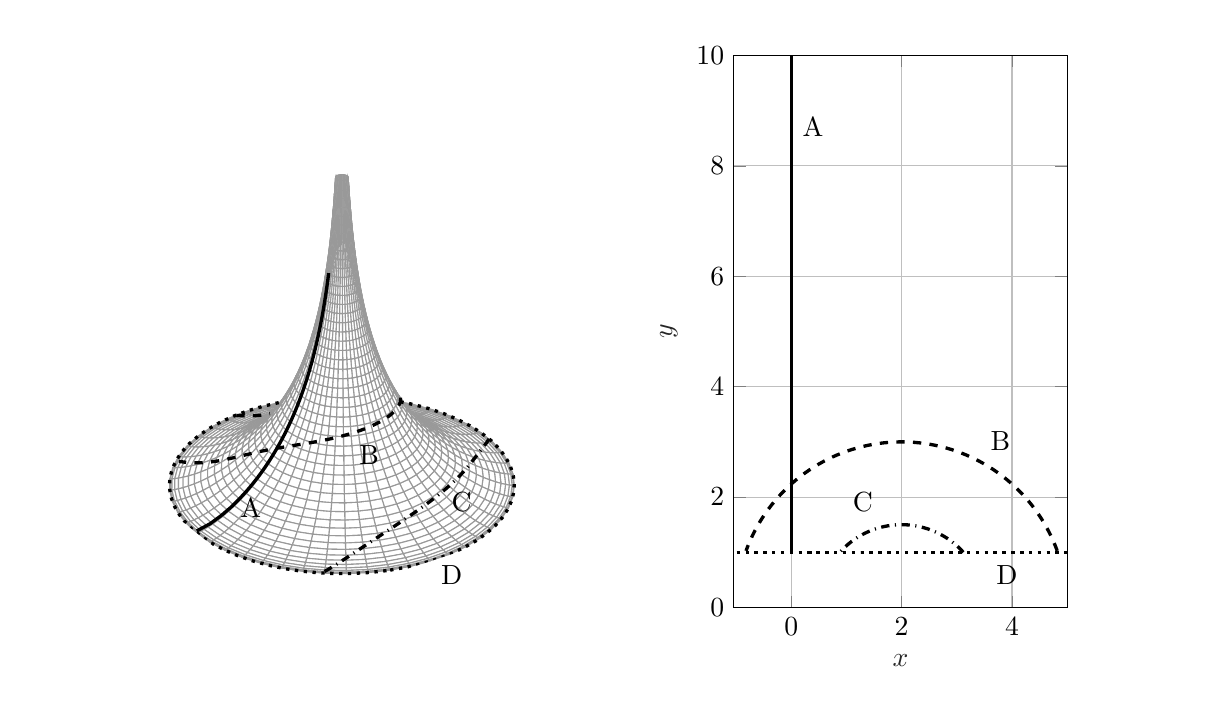
\begin{tikzpicture}

\begin{axis}[%
width=2.384in,
height=2.76in,
at={(0.379in,0.445in)},
scale only axis,
xmin=-1,
xmax=1,
tick align=outside,
ymin=-1,
ymax=1,
zmin=0,
zmax=3.00067070026093,
view={147.256768558952}{29.9750000078371},
axis line style={draw=none},
ticks=none,
axis x line*=bottom,
axis y line*=left,
axis z line*=left
]

\addplot3[%
surf,
fill=white, faceted color=white!60!black, z buffer=sort, colormap={mymap}{[1pt] rgb(0pt)=(0.2422,0.1504,0.6603); rgb(1pt)=(0.2444,0.1534,0.6728); rgb(2pt)=(0.2464,0.1569,0.6847); rgb(3pt)=(0.2484,0.1607,0.6961); rgb(4pt)=(0.2503,0.1648,0.7071); rgb(5pt)=(0.2522,0.1689,0.7179); rgb(6pt)=(0.254,0.1732,0.7286); rgb(7pt)=(0.2558,0.1773,0.7393); rgb(8pt)=(0.2576,0.1814,0.7501); rgb(9pt)=(0.2594,0.1854,0.761); rgb(11pt)=(0.2628,0.1932,0.7828); rgb(12pt)=(0.2645,0.1972,0.7937); rgb(13pt)=(0.2661,0.2011,0.8043); rgb(14pt)=(0.2676,0.2052,0.8148); rgb(15pt)=(0.2691,0.2094,0.8249); rgb(16pt)=(0.2704,0.2138,0.8346); rgb(17pt)=(0.2717,0.2184,0.8439); rgb(18pt)=(0.2729,0.2231,0.8528); rgb(19pt)=(0.274,0.228,0.8612); rgb(20pt)=(0.2749,0.233,0.8692); rgb(21pt)=(0.2758,0.2382,0.8767); rgb(22pt)=(0.2766,0.2435,0.884); rgb(23pt)=(0.2774,0.2489,0.8908); rgb(24pt)=(0.2781,0.2543,0.8973); rgb(25pt)=(0.2788,0.2598,0.9035); rgb(26pt)=(0.2794,0.2653,0.9094); rgb(27pt)=(0.2798,0.2708,0.915); rgb(28pt)=(0.2802,0.2764,0.9204); rgb(29pt)=(0.2806,0.2819,0.9255); rgb(30pt)=(0.2809,0.2875,0.9305); rgb(31pt)=(0.2811,0.293,0.9352); rgb(32pt)=(0.2813,0.2985,0.9397); rgb(33pt)=(0.2814,0.304,0.9441); rgb(34pt)=(0.2814,0.3095,0.9483); rgb(35pt)=(0.2813,0.315,0.9524); rgb(36pt)=(0.2811,0.3204,0.9563); rgb(37pt)=(0.2809,0.3259,0.96); rgb(38pt)=(0.2807,0.3313,0.9636); rgb(39pt)=(0.2803,0.3367,0.967); rgb(40pt)=(0.2798,0.3421,0.9702); rgb(41pt)=(0.2791,0.3475,0.9733); rgb(42pt)=(0.2784,0.3529,0.9763); rgb(43pt)=(0.2776,0.3583,0.9791); rgb(44pt)=(0.2766,0.3638,0.9817); rgb(45pt)=(0.2754,0.3693,0.984); rgb(46pt)=(0.2741,0.3748,0.9862); rgb(47pt)=(0.2726,0.3804,0.9881); rgb(48pt)=(0.271,0.386,0.9898); rgb(49pt)=(0.2691,0.3916,0.9912); rgb(50pt)=(0.267,0.3973,0.9924); rgb(51pt)=(0.2647,0.403,0.9935); rgb(52pt)=(0.2621,0.4088,0.9946); rgb(53pt)=(0.2591,0.4145,0.9955); rgb(54pt)=(0.2556,0.4203,0.9965); rgb(55pt)=(0.2517,0.4261,0.9974); rgb(56pt)=(0.2473,0.4319,0.9983); rgb(57pt)=(0.2424,0.4378,0.9991); rgb(58pt)=(0.2369,0.4437,0.9996); rgb(59pt)=(0.2311,0.4497,0.9995); rgb(60pt)=(0.225,0.4559,0.9985); rgb(61pt)=(0.2189,0.462,0.9968); rgb(62pt)=(0.2128,0.4682,0.9948); rgb(63pt)=(0.2066,0.4743,0.9926); rgb(64pt)=(0.2006,0.4803,0.9906); rgb(65pt)=(0.195,0.4861,0.9887); rgb(66pt)=(0.1903,0.4919,0.9867); rgb(67pt)=(0.1869,0.4975,0.9844); rgb(68pt)=(0.1847,0.503,0.9819); rgb(69pt)=(0.1831,0.5084,0.9793); rgb(70pt)=(0.1818,0.5138,0.9766); rgb(71pt)=(0.1806,0.5191,0.9738); rgb(72pt)=(0.1795,0.5244,0.9709); rgb(73pt)=(0.1785,0.5296,0.9677); rgb(74pt)=(0.1778,0.5349,0.9641); rgb(75pt)=(0.1773,0.5401,0.9602); rgb(76pt)=(0.1768,0.5452,0.956); rgb(77pt)=(0.1764,0.5504,0.9516); rgb(78pt)=(0.1755,0.5554,0.9473); rgb(79pt)=(0.174,0.5605,0.9432); rgb(80pt)=(0.1716,0.5655,0.9393); rgb(81pt)=(0.1686,0.5705,0.9357); rgb(82pt)=(0.1649,0.5755,0.9323); rgb(83pt)=(0.161,0.5805,0.9289); rgb(84pt)=(0.1573,0.5854,0.9254); rgb(85pt)=(0.154,0.5902,0.9218); rgb(86pt)=(0.1513,0.595,0.9182); rgb(87pt)=(0.1492,0.5997,0.9147); rgb(88pt)=(0.1475,0.6043,0.9113); rgb(89pt)=(0.1461,0.6089,0.908); rgb(90pt)=(0.1446,0.6135,0.905); rgb(91pt)=(0.1429,0.618,0.9022); rgb(92pt)=(0.1408,0.6226,0.8998); rgb(93pt)=(0.1383,0.6272,0.8975); rgb(94pt)=(0.1354,0.6317,0.8953); rgb(95pt)=(0.1321,0.6363,0.8932); rgb(96pt)=(0.1288,0.6408,0.891); rgb(97pt)=(0.1253,0.6453,0.8887); rgb(98pt)=(0.1219,0.6497,0.8862); rgb(99pt)=(0.1185,0.6541,0.8834); rgb(100pt)=(0.1152,0.6584,0.8804); rgb(101pt)=(0.1119,0.6627,0.877); rgb(102pt)=(0.1085,0.6669,0.8734); rgb(103pt)=(0.1048,0.671,0.8695); rgb(104pt)=(0.1009,0.675,0.8653); rgb(105pt)=(0.0964,0.6789,0.8609); rgb(106pt)=(0.0914,0.6828,0.8562); rgb(107pt)=(0.0855,0.6865,0.8513); rgb(108pt)=(0.0789,0.6902,0.8462); rgb(109pt)=(0.0713,0.6938,0.8409); rgb(110pt)=(0.0628,0.6972,0.8355); rgb(111pt)=(0.0535,0.7006,0.8299); rgb(112pt)=(0.0433,0.7039,0.8242); rgb(113pt)=(0.0328,0.7071,0.8183); rgb(114pt)=(0.0234,0.7103,0.8124); rgb(115pt)=(0.0155,0.7133,0.8064); rgb(116pt)=(0.0091,0.7163,0.8003); rgb(117pt)=(0.0046,0.7192,0.7941); rgb(118pt)=(0.0019,0.722,0.7878); rgb(119pt)=(0.0009,0.7248,0.7815); rgb(120pt)=(0.0018,0.7275,0.7752); rgb(121pt)=(0.0046,0.7301,0.7688); rgb(122pt)=(0.0094,0.7327,0.7623); rgb(123pt)=(0.0162,0.7352,0.7558); rgb(124pt)=(0.0253,0.7376,0.7492); rgb(125pt)=(0.0369,0.74,0.7426); rgb(126pt)=(0.0504,0.7423,0.7359); rgb(127pt)=(0.0638,0.7446,0.7292); rgb(128pt)=(0.077,0.7468,0.7224); rgb(129pt)=(0.0899,0.7489,0.7156); rgb(130pt)=(0.1023,0.751,0.7088); rgb(131pt)=(0.1141,0.7531,0.7019); rgb(132pt)=(0.1252,0.7552,0.695); rgb(133pt)=(0.1354,0.7572,0.6881); rgb(134pt)=(0.1448,0.7593,0.6812); rgb(135pt)=(0.1532,0.7614,0.6741); rgb(136pt)=(0.1609,0.7635,0.6671); rgb(137pt)=(0.1678,0.7656,0.6599); rgb(138pt)=(0.1741,0.7678,0.6527); rgb(139pt)=(0.1799,0.7699,0.6454); rgb(140pt)=(0.1853,0.7721,0.6379); rgb(141pt)=(0.1905,0.7743,0.6303); rgb(142pt)=(0.1954,0.7765,0.6225); rgb(143pt)=(0.2003,0.7787,0.6146); rgb(144pt)=(0.2061,0.7808,0.6065); rgb(145pt)=(0.2118,0.7828,0.5983); rgb(146pt)=(0.2178,0.7849,0.5899); rgb(147pt)=(0.2244,0.7869,0.5813); rgb(148pt)=(0.2318,0.7887,0.5725); rgb(149pt)=(0.2401,0.7905,0.5636); rgb(150pt)=(0.2491,0.7922,0.5546); rgb(151pt)=(0.2589,0.7937,0.5454); rgb(152pt)=(0.2695,0.7951,0.536); rgb(153pt)=(0.2809,0.7964,0.5266); rgb(154pt)=(0.2929,0.7975,0.517); rgb(155pt)=(0.3052,0.7985,0.5074); rgb(156pt)=(0.3176,0.7994,0.4975); rgb(157pt)=(0.3301,0.8002,0.4876); rgb(158pt)=(0.3424,0.8009,0.4774); rgb(159pt)=(0.3548,0.8016,0.4669); rgb(160pt)=(0.3671,0.8021,0.4563); rgb(161pt)=(0.3795,0.8026,0.4454); rgb(162pt)=(0.3921,0.8029,0.4344); rgb(163pt)=(0.405,0.8031,0.4233); rgb(164pt)=(0.4184,0.803,0.4122); rgb(165pt)=(0.4322,0.8028,0.4013); rgb(166pt)=(0.4463,0.8024,0.3904); rgb(167pt)=(0.4608,0.8018,0.3797); rgb(168pt)=(0.4753,0.8011,0.3691); rgb(169pt)=(0.4899,0.8002,0.3586); rgb(170pt)=(0.5044,0.7993,0.348); rgb(171pt)=(0.5187,0.7982,0.3374); rgb(172pt)=(0.5329,0.797,0.3267); rgb(173pt)=(0.547,0.7957,0.3159); rgb(175pt)=(0.5748,0.7929,0.2941); rgb(176pt)=(0.5886,0.7913,0.2833); rgb(177pt)=(0.6024,0.7896,0.2726); rgb(178pt)=(0.6161,0.7878,0.2622); rgb(179pt)=(0.6297,0.7859,0.2521); rgb(180pt)=(0.6433,0.7839,0.2423); rgb(181pt)=(0.6567,0.7818,0.2329); rgb(182pt)=(0.6701,0.7796,0.2239); rgb(183pt)=(0.6833,0.7773,0.2155); rgb(184pt)=(0.6963,0.775,0.2075); rgb(185pt)=(0.7091,0.7727,0.1998); rgb(186pt)=(0.7218,0.7703,0.1924); rgb(187pt)=(0.7344,0.7679,0.1852); rgb(188pt)=(0.7468,0.7654,0.1782); rgb(189pt)=(0.759,0.7629,0.1717); rgb(190pt)=(0.771,0.7604,0.1658); rgb(191pt)=(0.7829,0.7579,0.1608); rgb(192pt)=(0.7945,0.7554,0.157); rgb(193pt)=(0.806,0.7529,0.1546); rgb(194pt)=(0.8172,0.7505,0.1535); rgb(195pt)=(0.8281,0.7481,0.1536); rgb(196pt)=(0.8389,0.7457,0.1546); rgb(197pt)=(0.8495,0.7435,0.1564); rgb(198pt)=(0.86,0.7413,0.1587); rgb(199pt)=(0.8703,0.7392,0.1615); rgb(200pt)=(0.8804,0.7372,0.165); rgb(201pt)=(0.8903,0.7353,0.1695); rgb(202pt)=(0.9,0.7336,0.1749); rgb(203pt)=(0.9093,0.7321,0.1815); rgb(204pt)=(0.9184,0.7308,0.189); rgb(205pt)=(0.9272,0.7298,0.1973); rgb(206pt)=(0.9357,0.729,0.2061); rgb(207pt)=(0.944,0.7285,0.2151); rgb(208pt)=(0.9523,0.7284,0.2237); rgb(209pt)=(0.9606,0.7285,0.2312); rgb(210pt)=(0.9689,0.7292,0.2373); rgb(211pt)=(0.977,0.7304,0.2418); rgb(212pt)=(0.9842,0.733,0.2446); rgb(213pt)=(0.99,0.7365,0.2429); rgb(214pt)=(0.9946,0.7407,0.2394); rgb(215pt)=(0.9966,0.7458,0.2351); rgb(216pt)=(0.9971,0.7513,0.2309); rgb(217pt)=(0.9972,0.7569,0.2267); rgb(218pt)=(0.9971,0.7626,0.2224); rgb(219pt)=(0.9969,0.7683,0.2181); rgb(220pt)=(0.9966,0.774,0.2138); rgb(221pt)=(0.9962,0.7798,0.2095); rgb(222pt)=(0.9957,0.7856,0.2053); rgb(223pt)=(0.9949,0.7915,0.2012); rgb(224pt)=(0.9938,0.7974,0.1974); rgb(225pt)=(0.9923,0.8034,0.1939); rgb(226pt)=(0.9906,0.8095,0.1906); rgb(227pt)=(0.9885,0.8156,0.1875); rgb(228pt)=(0.9861,0.8218,0.1846); rgb(229pt)=(0.9835,0.828,0.1817); rgb(230pt)=(0.9807,0.8342,0.1787); rgb(231pt)=(0.9778,0.8404,0.1757); rgb(232pt)=(0.9748,0.8467,0.1726); rgb(233pt)=(0.972,0.8529,0.1695); rgb(234pt)=(0.9694,0.8591,0.1665); rgb(235pt)=(0.9671,0.8654,0.1636); rgb(236pt)=(0.9651,0.8716,0.1608); rgb(237pt)=(0.9634,0.8778,0.1582); rgb(238pt)=(0.9619,0.884,0.1557); rgb(239pt)=(0.9608,0.8902,0.1532); rgb(240pt)=(0.9601,0.8963,0.1507); rgb(241pt)=(0.9596,0.9023,0.148); rgb(242pt)=(0.9595,0.9084,0.145); rgb(243pt)=(0.9597,0.9143,0.1418); rgb(244pt)=(0.9601,0.9203,0.1382); rgb(245pt)=(0.9608,0.9262,0.1344); rgb(246pt)=(0.9618,0.932,0.1304); rgb(247pt)=(0.9629,0.9379,0.1261); rgb(248pt)=(0.9642,0.9437,0.1216); rgb(249pt)=(0.9657,0.9494,0.1168); rgb(250pt)=(0.9674,0.9552,0.1116); rgb(251pt)=(0.9692,0.9609,0.1061); rgb(252pt)=(0.9711,0.9667,0.1001); rgb(253pt)=(0.973,0.9724,0.0938); rgb(254pt)=(0.9749,0.9782,0.0872); rgb(255pt)=(0.9769,0.9839,0.0805)}, mesh/rows=50]
table[row sep=crcr, point meta=\thisrow{c}] {%
%
x	y	z	c\\
1	0	0	0\\
0.991790013823246	0.127877161684506	0	0\\
0.967294863039029	0.253654583909507	0	0\\
0.926916757346022	0.375267004879374	0	0\\
0.871318704123389	0.490717552003938	0	0\\
0.801413621867957	0.598110530491216	0	0\\
0.718349350097728	0.695682550603486	0	0\\
0.623489801858734	0.78183148246803	0	0\\
0.518392568310525	0.855142763005346	0	0\\
0.404783343122394	0.914412623015812	0	0\\
0.284527586631032	0.958667853036661	0	0\\
0.15959989503338	0.98718178341445	0	0\\
0.0320515775716553	0.999486216200688	0	0\\
-0.0960230259076818	0.995379112949198	0	0\\
-0.222520933956314	0.974927912181824	0	0\\
-0.345365054421307	0.93846842204976	0	0\\
-0.462538290240835	0.886599306373	0	0\\
-0.57211666012217	0.820172254596956	0	0\\
-0.672300890261317	0.740277997075315	0	0\\
-0.761445958369134	0.648228395307789	0	0\\
-0.838088104891841	0.545534901210549	0	0\\
-0.900968867902419	0.433883739117558	0	0\\
-0.949055747010669	0.315108218023621	0	0\\
-0.981559156991065	0.191158628701373	0	0\\
-0.997945392750336	0.0640702199807132	0	0\\
-0.997945392750336	-0.064070219980713	0	0\\
-0.981559156991065	-0.191158628701372	0	0\\
-0.949055747010669	-0.315108218023621	0	0\\
-0.900968867902419	-0.433883739117558	0	0\\
-0.838088104891841	-0.545534901210548	0	0\\
-0.761445958369135	-0.648228395307788	0	0\\
-0.672300890261317	-0.740277997075315	0	0\\
-0.57211666012217	-0.820172254596956	0	0\\
-0.462538290240835	-0.886599306373	0	0\\
-0.345365054421307	-0.938468422049761	0	0\\
-0.222520933956315	-0.974927912181824	0	0\\
-0.0960230259076816	-0.995379112949198	0	0\\
0.0320515775716549	-0.999486216200688	0	0\\
0.159599895033378	-0.98718178341445	0	0\\
0.284527586631032	-0.958667853036661	0	0\\
0.404783343122394	-0.914412623015812	0	0\\
0.518392568310524	-0.855142763005346	0	0\\
0.623489801858733	-0.78183148246803	0	0\\
0.718349350097727	-0.695682550603487	0	0\\
0.801413621867956	-0.598110530491217	0	0\\
0.871318704123389	-0.490717552003938	0	0\\
0.926916757346022	-0.375267004879375	0	0\\
0.967294863039029	-0.253654583909508	0	0\\
0.991790013823246	-0.127877161684507	0	0\\
1	-2.44929359829471e-16	0	0\\
0.996677281521151	0	0.000180848295413094	0.000180848295413094\\
0.988494574817178	0.127452261876354	0.000180848295413094	0.000180848295413094\\
0.964080814523114	0.252811761136307	0.000180848295413094	0.000180848295413094\\
0.923836873908034	0.374020098267759	0.000180848295413094	0.000180848295413094\\
0.868423557364232	0.489087035725999	0.000180848295413094	0.000180848295413094\\
0.798750750017375	0.596123177579159	0.000180848295413094	0.000180848295413094\\
0.715962477437889	0.693370993337184	0.000180848295413094	0.000180848295413094\\
0.621418120772724	0.779233676553888	0.000180848295413094	0.000180848295413094\\
0.516670095744502	0.852301364344654	0.000180848295413094	0.000180848295413094\\
0.403438362028271	0.911374287296025	0.000180848295413094	0.000180848295413094\\
0.283582181561191	0.955482469646297	0.000180848295413094	0.000180848295413094\\
0.15906958951293	0.983901656260716	0.000180848295413094	0.000180848295413094\\
0.0319450792025817	0.996165204880763	0.000180848295413094	0.000180848295413094\\
-0.0957039684251033	0.992071748377142	0.000180848295413094	0.000180848295413094\\
-0.221781559537127	0.971688501192472	0.000180848295413094	0.000180848295413094\\
-0.344217503573033	0.935350155682	0.000180848295413094	0.000180848295413094\\
-0.461001405716677	0.88365338647438	0.000180848295413094	0.000180848295413094\\
-0.570215677523525	0.817447053090767	0.000180848295413094	0.000180848295413094\\
-0.670067023669899	0.737818261694948	0.000180848295413094	0.000180848295413094\\
-0.758915887812616	0.646074514840185	0.000180848295413094	0.000180848295413094\\
-0.835303374058813	0.543722242313439	0.000180848295413094	0.000180848295413094\\
-0.897975201996172	0.43244206559992	0.000180848295413094	0.000180848295413094\\
-0.945902301942619	0.314061202124757	0.000180848295413094	0.000180848295413094\\
-0.978297712242048	0.190523462393395	0.000180848295413094	0.000180848295413094\\
-0.994629501152963	0.0638573326768394	0.000180848295413094	0.000180848295413094\\
-0.994629501152963	-0.0638573326768392	0.000180848295413094	0.000180848295413094\\
-0.978297712242048	-0.190523462393395	0.000180848295413094	0.000180848295413094\\
-0.945902301942619	-0.314061202124756	0.000180848295413094	0.000180848295413094\\
-0.897975201996172	-0.43244206559992	0.000180848295413094	0.000180848295413094\\
-0.835303374058813	-0.543722242313439	0.000180848295413094	0.000180848295413094\\
-0.758915887812617	-0.646074514840185	0.000180848295413094	0.000180848295413094\\
-0.670067023669899	-0.737818261694948	0.000180848295413094	0.000180848295413094\\
-0.570215677523525	-0.817447053090767	0.000180848295413094	0.000180848295413094\\
-0.461001405716677	-0.88365338647438	0.000180848295413094	0.000180848295413094\\
-0.344217503573033	-0.935350155682	0.000180848295413094	0.000180848295413094\\
-0.221781559537127	-0.971688501192472	0.000180848295413094	0.000180848295413094\\
-0.0957039684251031	-0.992071748377142	0.000180848295413094	0.000180848295413094\\
0.0319450792025813	-0.996165204880763	0.000180848295413094	0.000180848295413094\\
0.159069589512929	-0.983901656260716	0.000180848295413094	0.000180848295413094\\
0.283582181561191	-0.955482469646298	0.000180848295413094	0.000180848295413094\\
0.403438362028271	-0.911374287296025	0.000180848295413094	0.000180848295413094\\
0.516670095744501	-0.852301364344655	0.000180848295413094	0.000180848295413094\\
0.621418120772724	-0.779233676553888	0.000180848295413094	0.000180848295413094\\
0.715962477437888	-0.693370993337184	0.000180848295413094	0.000180848295413094\\
0.798750750017374	-0.59612317757916	0.000180848295413094	0.000180848295413094\\
0.868423557364232	-0.489087035725999	0.000180848295413094	0.000180848295413094\\
0.923836873908033	-0.37402009826776	0.000180848295413094	0.000180848295413094\\
0.964080814523114	-0.252811761136307	0.000180848295413094	0.000180848295413094\\
0.988494574817178	-0.127452261876355	0.000180848295413094	0.000180848295413094\\
0.996677281521151	-2.44115528519553e-16	0.000180848295413094	0.000180848295413094\\
0.986818657254952	0	0.00143534074664706	0.00143534074664706\\
0.978716889719926	0.126191568987079	0.00143534074664706	0.00143534074664706\\
0.954544617913788	0.250311075900144	0.00143534074664706	0.00143534074664706\\
0.914698749871315	0.370320481867152	0.00143534074664706	0.00143534074664706\\
0.859833553644168	0.484249235759963	0.00143534074664706	0.00143534074664706\\
0.790849914237565	0.590226630589389	0.00143534074664706	0.00143534074664706\\
0.708880541103407	0.686512520462233	0.00143534074664706	0.00143534074664706\\
0.615271369082392	0.77152589372875	0.00143534074664706	0.00143534074664706\\
0.511559458191139	0.843870833150225	0.00143534074664706	0.00143534074664706\\
0.399447755139211	0.902359436821443	0.00143534074664706	0.00143534074664706\\
0.280777130991228	0.946031323487125	0.00143534074664706	0.00143534074664706\\
0.157496154114871	0.974169401975597	0.00143534074664706	0.00143534074664706\\
0.0316290947421639	0.986311645815996	0.00143534074664706	0.00143534074664706\\
-0.094757313491776	0.982258679700153	0.00143534074664706	0.00143534074664706\\
-0.219587809257888	0.962077053219641	0.00143534074664706	0.00143534074664706\\
-0.340812679266818	0.926098148123318	0.00143534074664706	0.00143534074664706\\
-0.456441414504462	0.874912737038176	0.00143534074664706	0.00143534074664706\\
-0.564575394334947	0.809361282999135	0.00143534074664706	0.00143534074664706\\
-0.663439061798982	0.730520139069248	0.00143534074664706	0.00143534074664706\\
-0.751409078210039	0.639683874652164	0.00143534074664706	0.00143534074664706\\
-0.827040978330714	0.538344018698307	0.00143534074664706	0.00143534074664706\\
-0.88909288845198	0.428164568840747	0.00143534074664706	0.00143534074664706\\
-0.936545917925164	0.310954668600071	0.00143534074664706	0.00143534074664706\\
-0.968620889318226	0.188638901297786	0.00143534074664706	0.00143534074664706\\
-0.984791132487653	0.0632256884513968	0.00143534074664706	0.00143534074664706\\
-0.984791132487653	-0.0632256884513966	0.00143534074664706	0.00143534074664706\\
-0.968620889318226	-0.188638901297786	0.00143534074664706	0.00143534074664706\\
-0.936545917925164	-0.31095466860007	0.00143534074664706	0.00143534074664706\\
-0.88909288845198	-0.428164568840747	0.00143534074664706	0.00143534074664706\\
-0.827040978330714	-0.538344018698307	0.00143534074664706	0.00143534074664706\\
-0.75140907821004	-0.639683874652164	0.00143534074664706	0.00143534074664706\\
-0.663439061798982	-0.730520139069248	0.00143534074664706	0.00143534074664706\\
-0.564575394334948	-0.809361282999135	0.00143534074664706	0.00143534074664706\\
-0.456441414504462	-0.874912737038176	0.00143534074664706	0.00143534074664706\\
-0.340812679266818	-0.926098148123318	0.00143534074664706	0.00143534074664706\\
-0.219587809257888	-0.962077053219641	0.00143534074664706	0.00143534074664706\\
-0.0947573134917758	-0.982258679700153	0.00143534074664706	0.00143534074664706\\
0.0316290947421634	-0.986311645815996	0.00143534074664706	0.00143534074664706\\
0.15749615411487	-0.974169401975597	0.00143534074664706	0.00143534074664706\\
0.280777130991227	-0.946031323487125	0.00143534074664706	0.00143534074664706\\
0.399447755139211	-0.902359436821443	0.00143534074664706	0.00143534074664706\\
0.511559458191138	-0.843870833150226	0.00143534074664706	0.00143534074664706\\
0.615271369082391	-0.77152589372875	0.00143534074664706	0.00143534074664706\\
0.708880541103407	-0.686512520462233	0.00143534074664706	0.00143534074664706\\
0.790849914237564	-0.59022663058939	0.00143534074664706	0.00143534074664706\\
0.859833553644168	-0.484249235759963	0.00143534074664706	0.00143534074664706\\
0.914698749871315	-0.370320481867152	0.00143534074664706	0.00143534074664706\\
0.954544617913788	-0.250311075900144	0.00143534074664706	0.00143534074664706\\
0.978716889719926	-0.126191568987079	0.00143534074664706	0.00143534074664706\\
0.986818657254952	-2.41700861989233e-16	0.00143534074664706	0.00143534074664706\\
0.970744026930539	0	0.00478124968872615	0.00478124968872615\\
0.962774231888273	0.124135990886065	0.00478124968872615	0.00478124968872615\\
0.938995710575732	0.246233672233705	0.00478124968872615	0.00478124968872615\\
0.899798905655474	0.364288203490766	0.00478124968872615	0.00478124968872615\\
0.845827427580638	0.476361132517799	0.00478124968872615	0.00478124968872615\\
0.777967486529088	0.580612224918604	0.00478124968872615	0.00478124968872615\\
0.697333340856804	0.675329680638137	0.00478124968872615	0.00478124968872615\\
0.605249001006471	0.758958241672088	0.00478124968872615	0.00478124968872615\\
0.503226489292624	0.830124729360317	0.00478124968872615	0.00478124968872615\\
0.392941012537039	0.887660591942487	0.00478124968872615	0.00478124968872615\\
0.276203455219036	0.930621092145662	0.00478124968872615	0.00478124968872615\\
0.154930644802394	0.958300819744214	0.00478124968872615	0.00478124968872615\\
0.0311138774813852	0.970245274376223	0.00478124968872615	0.00478124968872615\\
-0.0932137788476785	0.966258328426852	0.00478124968872615	0.00478124968872615\\
-0.216010867505097	0.946405447438366	0.00478124968872615	0.00478124968872615\\
-0.335261063690025	0.911012615167733	0.00478124968872615	0.00478124968872615\\
-0.449006282477955	0.860660980942349	0.00478124968872615	0.00478124968872615\\
-0.555378830521046	0.796177317204148	0.00478124968872615	0.00478124968872615\\
-0.652632073521257	0.718620443928966	0.00478124968872615	0.00478124968872615\\
-0.739169115917237	0.629263842831804	0.00478124968872615	0.00478124968872615\\
-0.813569021865289	0.529574746832282	0.00478124968872615	0.00478124968872615\\
-0.874610146966643	0.421190048130658	0.00478124968872615	0.00478124968872615\\
-0.921290197634707	0.305889420483156	0.00478124968872615	0.00478124968872615\\
-0.952842688728052	0.18556609700809	0.00478124968872615	0.00478124968872615\\
-0.96874952921524	0.062195783350403	0.00478124968872615	0.00478124968872615\\
-0.96874952921524	-0.0621957833504028	0.00478124968872615	0.00478124968872615\\
-0.952842688728052	-0.18556609700809	0.00478124968872615	0.00478124968872615\\
-0.921290197634707	-0.305889420483156	0.00478124968872615	0.00478124968872615\\
-0.874610146966643	-0.421190048130658	0.00478124968872615	0.00478124968872615\\
-0.813569021865289	-0.529574746832282	0.00478124968872615	0.00478124968872615\\
-0.739169115917237	-0.629263842831804	0.00478124968872615	0.00478124968872615\\
-0.652632073521257	-0.718620443928965	0.00478124968872615	0.00478124968872615\\
-0.555378830521046	-0.796177317204148	0.00478124968872615	0.00478124968872615\\
-0.449006282477955	-0.860660980942349	0.00478124968872615	0.00478124968872615\\
-0.335261063690025	-0.911012615167733	0.00478124968872615	0.00478124968872615\\
-0.216010867505097	-0.946405447438366	0.00478124968872615	0.00478124968872615\\
-0.0932137788476783	-0.966258328426852	0.00478124968872615	0.00478124968872615\\
0.0311138774813848	-0.970245274376223	0.00478124968872615	0.00478124968872615\\
0.154930644802393	-0.958300819744215	0.00478124968872615	0.00478124968872615\\
0.276203455219036	-0.930621092145662	0.00478124968872615	0.00478124968872615\\
0.392941012537039	-0.887660591942487	0.00478124968872615	0.00478124968872615\\
0.503226489292623	-0.830124729360317	0.00478124968872615	0.00478124968872615\\
0.605249001006471	-0.758958241672088	0.00478124968872615	0.00478124968872615\\
0.697333340856803	-0.675329680638137	0.00478124968872615	0.00478124968872615\\
0.777967486529088	-0.580612224918605	0.00478124968872615	0.00478124968872615\\
0.845827427580638	-0.476361132517799	0.00478124968872615	0.00478124968872615\\
0.899798905655474	-0.364288203490766	0.00478124968872615	0.00478124968872615\\
0.938995710575732	-0.246233672233706	0.00478124968872615	0.00478124968872615\\
0.962774231888273	-0.124135990886066	0.00478124968872615	0.00478124968872615\\
0.970744026930539	-2.37763713074379e-16	0.00478124968872615	0.00478124968872615\\
0.948958838413527	0	0.0111306709055737	0.0111306709055737\\
0.941167899467844	0.121350162811748	0.0111306709055737	0.0111306709055737\\
0.917923009632889	0.240707759305033	0.0111306709055737	0.0111306709055737\\
0.879605849357114	0.356112941045254	0.0111306709055737	0.0111306709055737\\
0.826845585352911	0.465670758138787	0.0111306709055737	0.0111306709055737\\
0.760508539696594	0.567582274257843	0.0111306709055737	0.0111306709055737\\
0.681683964843852	0.660174105125244	0.0111306709055737	0.0111306709055737\\
0.591666158134544	0.741925895437988	0.0111306709055737	0.0111306709055737\\
0.491933209466161	0.811495283059287	0.0111306709055737	0.0111306709055737\\
0.384122731098571	0.867739940567752	0.0111306709055737	0.0111306709055737\\
0.270004968105989	0.90973633224206	0.0111306709055737	0.0111306709055737\\
0.151453731001797	0.936794878491971	0.0111306709055737	0.0111306709055737\\
0.0304156278217191	0.948471278736136	0.0111306709055737	0.0111306709055737\\
-0.0911218991263057	0.944573806805358	0.0111306709055737	0.0111306709055737\\
-0.211163207009877	0.925166459080989	0.0111306709055737	0.0111306709055737\\
-0.327737220872269	0.890567903676116	0.0111306709055737	0.0111306709055737\\
-0.438929798628722	0.841346247913961	0.0111306709055737	0.0111306709055737\\
-0.542915161226561	0.778309710021331	0.0111306709055737	0.0111306709055737\\
-0.637985871886759	0.702493348207684	0.0111306709055737	0.0111306709055737\\
-0.722580872168649	0.615142065037944	0.0111306709055737	0.0111306709055737\\
-0.795311114506355	0.517690166166801	0.0111306709055737	0.0111306709055737\\
-0.85498237033143	0.411737809079516	0.0111306709055737	0.0111306709055737\\
-0.900614839272926	0.299024728550252	0.0111306709055737	0.0111306709055737\\
-0.931459237452402	0.181401670245177	0.0111306709055737	0.0111306709055737\\
-0.94700910070449	0.0608000015297968	0.0111306709055737	0.0111306709055737\\
-0.94700910070449	-0.0608000015297966	0.0111306709055737	0.0111306709055737\\
-0.931459237452402	-0.181401670245177	0.0111306709055737	0.0111306709055737\\
-0.900614839272927	-0.299024728550251	0.0111306709055737	0.0111306709055737\\
-0.85498237033143	-0.411737809079516	0.0111306709055737	0.0111306709055737\\
-0.795311114506355	-0.5176901661668	0.0111306709055737	0.0111306709055737\\
-0.722580872168649	-0.615142065037943	0.0111306709055737	0.0111306709055737\\
-0.63798587188676	-0.702493348207684	0.0111306709055737	0.0111306709055737\\
-0.542915161226561	-0.778309710021331	0.0111306709055737	0.0111306709055737\\
-0.438929798628722	-0.841346247913961	0.0111306709055737	0.0111306709055737\\
-0.327737220872268	-0.890567903676117	0.0111306709055737	0.0111306709055737\\
-0.211163207009878	-0.925166459080989	0.0111306709055737	0.0111306709055737\\
-0.0911218991263055	-0.944573806805358	0.0111306709055737	0.0111306709055737\\
0.0304156278217187	-0.948471278736136	0.0111306709055737	0.0111306709055737\\
0.151453731001796	-0.936794878491971	0.0111306709055737	0.0111306709055737\\
0.270004968105988	-0.90973633224206	0.0111306709055737	0.0111306709055737\\
0.384122731098571	-0.867739940567752	0.0111306709055737	0.0111306709055737\\
0.49193320946616	-0.811495283059288	0.0111306709055737	0.0111306709055737\\
0.591666158134544	-0.741925895437988	0.0111306709055737	0.0111306709055737\\
0.681683964843851	-0.660174105125245	0.0111306709055737	0.0111306709055737\\
0.760508539696593	-0.567582274257844	0.0111306709055737	0.0111306709055737\\
0.826845585352911	-0.465670758138787	0.0111306709055737	0.0111306709055737\\
0.879605849357114	-0.356112941045255	0.0111306709055737	0.0111306709055737\\
0.917923009632889	-0.240707759305033	0.0111306709055737	0.0111306709055737\\
0.941167899467844	-0.121350162811748	0.0111306709055737	0.0111306709055737\\
0.948958838413527	-2.32427880797143e-16	0.0111306709055737	0.0111306709055737\\
0.922116636293008	0	0.021251248082997	0.021251248082997\\
0.914546071455688	0.117917658191214	0.021251248082997	0.021251248082997\\
0.891958685409056	0.233899111694937	0.021251248082997	0.021251248082997\\
0.854725362407536	0.34603994825112	0.021251248082997	0.021251248082997\\
0.803457472585443	0.45249881842381	0.021251248082997	0.021251248082997\\
0.738996833276277	0.551527670507987	0.021251248082997	0.021251248082997\\
0.662401886395385	0.641500453490227	0.021251248082997	0.021251248082997\\
0.57493031885297	0.720939816761396	0.021251248082997	0.021251248082997\\
0.478018411369795	0.788541368172799	0.021251248082997	0.021251248082997\\
0.37325745478746	0.843195092119208	0.021251248082997	0.021251248082997\\
0.262367621116775	0.884003575964405	0.021251248082997	0.021251248082997\\
0.147169718360897	0.910296745531866	0.021251248082997	0.021251248082997\\
0.0295552928982592	0.921642867704205	0.021251248082997	0.021251248082997\\
-0.0885444296566679	0.917855639469033	0.021251248082997	0.021251248082997\\
-0.205190255124575	0.898997247009268	0.021251248082997	0.021251248082997\\
-0.318466862276128	0.865377344607732	0.021251248082997	0.021251248082997\\
-0.426514252353598	0.817547970132385	0.021251248082997	0.021251248082997\\
-0.527558290199045	0.756294480589798	0.021251248082997	0.021251248082997\\
-0.61993983550456	0.682622656584815	0.021251248082997	0.021251248082997\\
-0.702141985850252	0.597742187430833	0.021251248082997	0.021251248082997\\
-0.772814984200046	0.50304680808471	0.021251248082997	0.021251248082997\\
-0.830798381874898	0.400091414057316	0.021251248082997	0.021251248082997\\
-0.875140093088026	0.290566530072225	0.021251248082997	0.021251248082997\\
-0.905112028167202	0.176270551696494	0.021251248082997	0.021251248082997\\
-0.920222048767045	0.0590802157351684	0.021251248082997	0.021251248082997\\
-0.920222048767045	-0.0590802157351681	0.021251248082997	0.021251248082997\\
-0.905112028167202	-0.176270551696493	0.021251248082997	0.021251248082997\\
-0.875140093088026	-0.290566530072225	0.021251248082997	0.021251248082997\\
-0.830798381874898	-0.400091414057316	0.021251248082997	0.021251248082997\\
-0.772814984200046	-0.503046808084709	0.021251248082997	0.021251248082997\\
-0.702141985850252	-0.597742187430832	0.021251248082997	0.021251248082997\\
-0.61993983550456	-0.682622656584815	0.021251248082997	0.021251248082997\\
-0.527558290199046	-0.756294480589797	0.021251248082997	0.021251248082997\\
-0.426514252353598	-0.817547970132385	0.021251248082997	0.021251248082997\\
-0.318466862276128	-0.865377344607732	0.021251248082997	0.021251248082997\\
-0.205190255124575	-0.898997247009268	0.021251248082997	0.021251248082997\\
-0.0885444296566677	-0.917855639469033	0.021251248082997	0.021251248082997\\
0.0295552928982588	-0.921642867704205	0.021251248082997	0.021251248082997\\
0.147169718360896	-0.910296745531866	0.021251248082997	0.021251248082997\\
0.262367621116775	-0.884003575964405	0.021251248082997	0.021251248082997\\
0.37325745478746	-0.843195092119208	0.021251248082997	0.021251248082997\\
0.478018411369794	-0.788541368172799	0.021251248082997	0.021251248082997\\
0.574930318852969	-0.720939816761396	0.021251248082997	0.021251248082997\\
0.662401886395385	-0.641500453490228	0.021251248082997	0.021251248082997\\
0.738996833276276	-0.551527670507988	0.021251248082997	0.021251248082997\\
0.803457472585443	-0.45249881842381	0.021251248082997	0.021251248082997\\
0.854725362407536	-0.346039948251121	0.021251248082997	0.021251248082997\\
0.891958685409056	-0.233899111694938	0.021251248082997	0.021251248082997\\
0.914546071455688	-0.117917658191214	0.021251248082997	0.021251248082997\\
0.922116636293008	-2.25853437415351e-16	0.021251248082997	0.021251248082997\\
0.890973941781643	0	0.0357414777260489	0.0357414777260489\\
0.883659058035767	0.113935218809893	0.0357414777260489	0.0357414777260489\\
0.861834516987018	0.225999624476836	0.0357414777260489	0.0357414777260489\\
0.825858676996043	0.334353122557967	0.0357414777260489	0.0357414777260489\\
0.776322260360889	0.437216551610387	0.0357414777260489	0.0357414777260489\\
0.714038653673196	0.532900896972868	0.0357414777260489	0.0357414777260489\\
0.640030552032854	0.619835024339895	0.0357414777260489	0.0357414777260489\\
0.555513166422731	0.696591477743526	0.0357414777260489	0.0357414777260489\\
0.461874269977938	0.761909918340918	0.0357414777260489	0.0357414777260489\\
0.36065141078931	0.81471781914329	0.0357414777260489	0.0357414777260489\\
0.253506665406269	0.854148075879418	0.0357414777260489	0.0357414777260489\\
0.142199347585827	0.879553244823804	0.0357414777260489	0.0357414777260489\\
0.0285571204093378	0.890516173804746	0.0357414777260489	0.0357414777260489\\
-0.085554013894768	0.886856851831462	0.0357414777260489	0.0357414777260489\\
-0.19826035365599	0.868635364869586	0.0357414777260489	0.0357414777260489\\
-0.307711263891384	0.836150909231273	0.0357414777260489	0.0357414777260489\\
-0.412109563680818	0.789936878780022	0.0357414777260489	0.0357414777260489\\
-0.509741035827998	0.730752106618187	0.0357414777260489	0.0357414777260489\\
-0.599002574259433	0.659568405068413	0.0357414777260489	0.0357414777260489\\
-0.678428506981848	0.577554608542169	0.0357414777260489	0.0357414777260489\\
-0.74671466237579	0.486057381311022	0.0357414777260489	0.0357414777260489\\
-0.802739783657562	0.386579105316529	0.0357414777260489	0.0357414777260489\\
-0.845583939884617	0.280753211100295	0.0357414777260489	0.0357414777260489\\
-0.874543631196196	0.170317356919635	0.0357414777260489	0.0357414777260489\\
-0.889143340261597	0.057084896447033	0.0357414777260489	0.0357414777260489\\
-0.889143340261597	-0.0570848964470328	0.0357414777260489	0.0357414777260489\\
-0.874543631196196	-0.170317356919635	0.0357414777260489	0.0357414777260489\\
-0.845583939884617	-0.280753211100294	0.0357414777260489	0.0357414777260489\\
-0.802739783657562	-0.386579105316529	0.0357414777260489	0.0357414777260489\\
-0.74671466237579	-0.486057381311021	0.0357414777260489	0.0357414777260489\\
-0.678428506981848	-0.577554608542169	0.0357414777260489	0.0357414777260489\\
-0.599002574259433	-0.659568405068413	0.0357414777260489	0.0357414777260489\\
-0.509741035827998	-0.730752106618187	0.0357414777260489	0.0357414777260489\\
-0.412109563680819	-0.789936878780022	0.0357414777260489	0.0357414777260489\\
-0.307711263891384	-0.836150909231273	0.0357414777260489	0.0357414777260489\\
-0.19826035365599	-0.868635364869586	0.0357414777260489	0.0357414777260489\\
-0.0855540138947678	-0.886856851831462	0.0357414777260489	0.0357414777260489\\
0.0285571204093374	-0.890516173804746	0.0357414777260489	0.0357414777260489\\
0.142199347585826	-0.879553244823805	0.0357414777260489	0.0357414777260489\\
0.253506665406268	-0.854148075879418	0.0357414777260489	0.0357414777260489\\
0.36065141078931	-0.81471781914329	0.0357414777260489	0.0357414777260489\\
0.461874269977937	-0.761909918340919	0.0357414777260489	0.0357414777260489\\
0.555513166422731	-0.696591477743526	0.0357414777260489	0.0357414777260489\\
0.640030552032853	-0.619835024339896	0.0357414777260489	0.0357414777260489\\
0.714038653673196	-0.532900896972869	0.0357414777260489	0.0357414777260489\\
0.776322260360889	-0.437216551610387	0.0357414777260489	0.0357414777260489\\
0.825858676996043	-0.334353122557967	0.0357414777260489	0.0357414777260489\\
0.861834516987018	-0.225999624476836	0.0357414777260489	0.0357414777260489\\
0.883659058035767	-0.113935218809893	0.0357414777260489	0.0357414777260489\\
0.890973941781643	-2.18225677185318e-16	0.0357414777260489	0.0357414777260489\\
0.856342883234364	0	0.0550209162433916	0.0550209162433916\\
0.849312320000449	0.109506697336737	0.0550209162433916	0.0550209162433916\\
0.828336071952632	0.217215297730681	0.0550209162433916	0.0550209162433916\\
0.79375856850394	0.321357228941128	0.0550209162433916	0.0550209162433916\\
0.746147571305053	0.420222483336761	0.0550209162433916	0.0550209162433916\\
0.686284851613701	0.512187696173683	0.0550209162433916	0.0550209162433916\\
0.61515335363222	0.595742801199626	0.0550209162433916	0.0550209162433916\\
0.533921054590931	0.66951582590007	0.0550209162433916	0.0550209162433916\\
0.443921786594302	0.732295419248999	0.0550209162433916	0.0550209162433916\\
0.346633335134676	0.783050742059259	0.0550209162433916	0.0550209162433916\\
0.243653173895334	0.820948393333512	0.0550209162433916	0.0550209162433916\\
0.136672234276786	0.845366094685572	0.0550209162433916	0.0550209162433916\\
0.0274471403499212	0.855902908134302	0.0550209162433916	0.0550209162433916\\
-0.0822286348626723	0.85238581949418	0.0550209162433916	0.0550209162433916\\
-0.190554218164154	0.834872579263442	0.0550209162433916	0.0550209162433916\\
-0.295750906471536	0.803650754362496	0.0550209162433916	0.0550209162433916\\
-0.39609137307113	0.759233006293043	0.0550209162433916	0.0550209162433916\\
-0.489928030275434	0.702348673250386	0.0550209162433916	0.0550209162433916\\
-0.575720082767406	0.633931794410436	0.0550209162433916	0.0550209162433916\\
-0.652058827416978	0.555105773032257	0.0550209162433916	0.0550209162433916\\
-0.717690784147503	0.467164930207615	0.0550209162433916	0.0550209162433916\\
-0.771538278043959	0.371553252144437	0.0550209162433916	0.0550209162433916\\
-0.812717134745259	0.269840679953191	0.0550209162433916	0.0550209162433916\\
-0.840551198562821	0.163697331257261	0.0550209162433916	0.0550209162433916\\
-0.854583434938273	0.054866076907744	0.0550209162433916	0.0550209162433916\\
-0.854583434938273	-0.0548660769077437	0.0550209162433916	0.0550209162433916\\
-0.840551198562821	-0.16369733125726	0.0550209162433916	0.0550209162433916\\
-0.81271713474526	-0.26984067995319	0.0550209162433916	0.0550209162433916\\
-0.771538278043959	-0.371553252144436	0.0550209162433916	0.0550209162433916\\
-0.717690784147503	-0.467164930207615	0.0550209162433916	0.0550209162433916\\
-0.652058827416979	-0.555105773032257	0.0550209162433916	0.0550209162433916\\
-0.575720082767406	-0.633931794410436	0.0550209162433916	0.0550209162433916\\
-0.489928030275434	-0.702348673250386	0.0550209162433916	0.0550209162433916\\
-0.39609137307113	-0.759233006293042	0.0550209162433916	0.0550209162433916\\
-0.295750906471536	-0.803650754362496	0.0550209162433916	0.0550209162433916\\
-0.190554218164154	-0.834872579263442	0.0550209162433916	0.0550209162433916\\
-0.0822286348626721	-0.85238581949418	0.0550209162433916	0.0550209162433916\\
0.0274471403499208	-0.855902908134302	0.0550209162433916	0.0550209162433916\\
0.136672234276785	-0.845366094685572	0.0550209162433916	0.0550209162433916\\
0.243653173895333	-0.820948393333512	0.0550209162433916	0.0550209162433916\\
0.346633335134676	-0.783050742059259	0.0550209162433916	0.0550209162433916\\
0.443921786594302	-0.732295419248999	0.0550209162433916	0.0550209162433916\\
0.53392105459093	-0.66951582590007	0.0550209162433916	0.0550209162433916\\
0.615153353632219	-0.595742801199627	0.0550209162433916	0.0550209162433916\\
0.6862848516137	-0.512187696173684	0.0550209162433916	0.0550209162433916\\
0.746147571305053	-0.420222483336761	0.0550209162433916	0.0550209162433916\\
0.79375856850394	-0.321357228941128	0.0550209162433916	0.0550209162433916\\
0.828336071952632	-0.217215297730681	0.0550209162433916	0.0550209162433916\\
0.849312320000449	-0.109506697336737	0.0550209162433916	0.0550209162433916\\
0.856342883234364	-2.09743514185116e-16	0.0550209162433916	0.0550209162433916\\
0.819046488706006	0	0.0793340686584179	0.0793340686584179\\
0.812322128355611	0.104737340263385	0.0793340686584179	0.0793340686584179\\
0.792259461115474	0.207754896295265	0.0793340686584179	0.0793340686584179\\
0.759187915427016	0.307361122673671	0.0793340686584179	0.0793340686584179\\
0.713650525156129	0.401920487915232	0.0793340686584179	0.0793340686584179\\
0.656395012992113	0.489880329856917	0.0793340686584179	0.0793340686584179\\
0.588361512861785	0.569796350325824	0.0793340686584179	0.0793340686584179\\
0.510667132956399	0.640356330475251	0.0793340686584179	0.0793340686584179\\
0.424587612846024	0.700401677381881	0.0793340686584179	0.0793340686584179\\
0.331536375871075	0.74894644810955	0.0793340686584179	0.0793340686584179\\
0.233041320770141	0.785193538865002	0.0793340686584179	0.0793340686584179\\
0.130719733624937	0.808547773420138	0.0793340686584179	0.0793340686584179\\
0.0262517320675525	0.818625675889225	0.0793340686584179	0.0793340686584179\\
-0.0786473222046126	0.81526176739234	0.0793340686584179	0.0793340686584179\\
-0.1822549896205	0.798511283214	0.0793340686584179	0.0793340686584179\\
-0.282870035145531	0.768649265841322	0.0793340686584179	0.0793340686584179\\
-0.378840362513836	0.726166048773986	0.0793340686584179	0.0793340686584179\\
-0.468590141603271	0.671759205261725	0.0793340686584179	0.0793340686584179\\
-0.550645683522453	0.606322094170852	0.0793340686584179	0.0793340686584179\\
-0.623659638541619	0.530929191056373	0.0793340686584179	0.0793340686584179\\
-0.686433119537933	0.446818445303078	0.0793340686584179	0.0793340686584179\\
-0.737935387688902	0.355370953030869	0.0793340686584179	0.0793340686584179\\
-0.777320777175344	0.258088279534654	0.0793340686584179	0.0793340686584179\\
-0.803942580990759	0.156567803623714	0.0793340686584179	0.0793340686584179\\
-0.817363669852499	0.0524764887058246	0.0793340686584179	0.0793340686584179\\
-0.817363669852499	-0.0524764887058244	0.0793340686584179	0.0793340686584179\\
-0.803942580990759	-0.156567803623714	0.0793340686584179	0.0793340686584179\\
-0.777320777175344	-0.258088279534653	0.0793340686584179	0.0793340686584179\\
-0.737935387688902	-0.355370953030869	0.0793340686584179	0.0793340686584179\\
-0.686433119537933	-0.446818445303078	0.0793340686584179	0.0793340686584179\\
-0.623659638541619	-0.530929191056373	0.0793340686584179	0.0793340686584179\\
-0.550645683522454	-0.606322094170852	0.0793340686584179	0.0793340686584179\\
-0.468590141603271	-0.671759205261725	0.0793340686584179	0.0793340686584179\\
-0.378840362513836	-0.726166048773986	0.0793340686584179	0.0793340686584179\\
-0.28287003514553	-0.768649265841323	0.0793340686584179	0.0793340686584179\\
-0.182254989620501	-0.798511283214	0.0793340686584179	0.0793340686584179\\
-0.0786473222046124	-0.81526176739234	0.0793340686584179	0.0793340686584179\\
0.0262517320675521	-0.818625675889225	0.0793340686584179	0.0793340686584179\\
0.130719733624936	-0.808547773420139	0.0793340686584179	0.0793340686584179\\
0.233041320770141	-0.785193538865002	0.0793340686584179	0.0793340686584179\\
0.331536375871075	-0.74894644810955	0.0793340686584179	0.0793340686584179\\
0.424587612846023	-0.700401677381881	0.0793340686584179	0.0793340686584179\\
0.510667132956399	-0.640356330475251	0.0793340686584179	0.0793340686584179\\
0.588361512861785	-0.569796350325824	0.0793340686584179	0.0793340686584179\\
0.656395012992112	-0.489880329856918	0.0793340686584179	0.0793340686584179\\
0.713650525156129	-0.401920487915232	0.0793340686584179	0.0793340686584179\\
0.759187915427016	-0.307361122673671	0.0793340686584179	0.0793340686584179\\
0.792259461115474	-0.207754896295265	0.0793340686584179	0.0793340686584179\\
0.812322128355611	-0.104737340263385	0.0793340686584179	0.0793340686584179\\
0.819046488706006	-2.00608532149338e-16	0.0793340686584179	0.0793340686584179\\
0.779880351526415	0	0.108765257576638	0.108765257576638\\
0.773477544620862	0.0997288858067128	0.108765257576638	0.108765257576638\\
0.754374257816574	0.197820226065633	0.108765257576638	0.108765257576638\\
0.722884166554741	0.292663363681591	0.108765257576638	0.108765257576638\\
0.67952433726329	0.382700976957013	0.108765257576638	0.108765257576638\\
0.62500673714044	0.46645465077114	0.108765257576638	0.108765257576638\\
0.560226543672988	0.54254915211544	0.108765257576638	0.108765257576638\\
0.486247445846724	0.609735011381586	0.108765257576638	0.108765257576638\\
0.404284178402694	0.666909038617879	0.108765257576638	0.108765257576638\\
0.31568257592633	0.713132437877763	0.108765257576638	0.108765257576638\\
0.221897474280772	0.747646222223305	0.108765257576638	0.108765257576638\\
0.124468822242211	0.769883676269735	0.108765257576638	0.108765257576638\\
0.0249963955835587	0.779479661636399	0.108765257576638	0.108765257576638\\
-0.0748864711995129	0.776276612508872	0.108765257576638	0.108765257576638\\
-0.173539704195837	0.760327122865275	0.108765257576638	0.108765257576638\\
-0.269343420047029	0.731893082884608	0.108765257576638	0.108765257576638\\
-0.36072452438745	0.691441378717251	0.108765257576638	0.108765257576638\\
-0.446182542010197	0.639636226227287	0.108765257576638	0.108765257576638\\
-0.524314254628518	0.577328264586368	0.108765257576638	0.108765257576638\\
-0.593836741681289	0.505540588802042	0.108765257576638	0.108765257576638\\
-0.653608445853156	0.425451950526011	0.108765257576638	0.108765257576638\\
-0.702647917414095	0.338377402984597	0.108765257576638	0.108765257576638\\
-0.740149929596845	0.245746707841124	0.108765257576638	0.108765257576638\\
-0.765498700398164	0.149080858548934	0.108765257576638	0.108765257576638\\
-0.778278003702299	0.0499671056809334	0.108765257576638	0.108765257576638\\
-0.778278003702299	-0.0499671056809332	0.108765257576638	0.108765257576638\\
-0.765498700398164	-0.149080858548934	0.108765257576638	0.108765257576638\\
-0.740149929596845	-0.245746707841124	0.108765257576638	0.108765257576638\\
-0.702647917414095	-0.338377402984597	0.108765257576638	0.108765257576638\\
-0.653608445853156	-0.425451950526011	0.108765257576638	0.108765257576638\\
-0.593836741681289	-0.505540588802042	0.108765257576638	0.108765257576638\\
-0.524314254628518	-0.577328264586368	0.108765257576638	0.108765257576638\\
-0.446182542010197	-0.639636226227286	0.108765257576638	0.108765257576638\\
-0.36072452438745	-0.691441378717251	0.108765257576638	0.108765257576638\\
-0.269343420047029	-0.731893082884608	0.108765257576638	0.108765257576638\\
-0.173539704195837	-0.760327122865275	0.108765257576638	0.108765257576638\\
-0.0748864711995128	-0.776276612508872	0.108765257576638	0.108765257576638\\
0.0249963955835584	-0.779479661636399	0.108765257576638	0.108765257576638\\
0.12446882224221	-0.769883676269735	0.108765257576638	0.108765257576638\\
0.221897474280772	-0.747646222223305	0.108765257576638	0.108765257576638\\
0.31568257592633	-0.713132437877763	0.108765257576638	0.108765257576638\\
0.404284178402693	-0.66690903861788	0.108765257576638	0.108765257576638\\
0.486247445846724	-0.609735011381586	0.108765257576638	0.108765257576638\\
0.560226543672987	-0.542549152115441	0.108765257576638	0.108765257576638\\
0.625006737140439	-0.466454650771141	0.108765257576638	0.108765257576638\\
0.67952433726329	-0.382700976957013	0.108765257576638	0.108765257576638\\
0.72288416655474	-0.292663363681592	0.108765257576638	0.108765257576638\\
0.754374257816574	-0.197820226065633	0.108765257576638	0.108765257576638\\
0.773477544620862	-0.0997288858067133	0.108765257576638	0.108765257576638\\
0.779880351526415	-1.91015595242947e-16	0.108765257576638	0.108765257576638\\
0.739582863872753	0	0.143261015624456	0.143261015624456\\
0.733510898783794	0.094575757462546	0.143261015624456	0.143261015624456\\
0.715394705015808	0.187598583602245	0.143261015624456	0.143261015624456\\
0.685531749969616	0.277541046185638	0.143261015624456	0.143261015624456\\
0.644412382541472	0.362926292463699	0.143261015624456	0.143261015624456\\
0.592711781607739	0.442352299053145	0.143261015624456	0.143261015624456\\
0.531278869606408	0.514514893121628	0.143261015624456	0.143261015624456\\
0.461122373254137	0.578229166869586	0.143261015624456	0.143261015624456\\
0.38339426028145	0.632448933683553	0.143261015624456	0.143261015624456\\
0.299370824154447	0.676283906491431	0.143261015624456	0.143261015624456\\
0.210431727371382	0.709014316251597	0.143261015624456	0.143261015624456\\
0.118037347442578	0.730102730540671	0.143261015624456	0.143261015624456\\
0.0237047975320845	0.739202878179046	0.143261015624456	0.143261015624456\\
-0.0710169844985308	0.736165334994088	0.143261015624456	0.143261015624456\\
-0.164572669607051	0.721039977360917	0.143261015624456	0.143261015624456\\
-0.25542607603048	0.694075163233705	0.143261015624456	0.143261015624456\\
-0.342085393347123	0.65571365411494	0.143261015624456	0.143261015624456\\
-0.423127677962469	0.606585344923789	0.143261015624456	0.143261015624456\\
-0.497222217803666	0.547496921138947	0.143261015624456	0.143261015624456\\
-0.563152382574977	0.479418613045373	0.143261015624456	0.143261015624456\\
-0.619835600793596	0.403468264579837	0.143261015624456	0.143261015624456\\
-0.666341135583463	0.320892978364382	0.143261015624456	0.143261015624456\\
-0.701905367349045	0.23304863831575	0.143261015624456	0.143261015624456\\
-0.725944332387977	0.141377646068949	0.143261015624456	0.143261015624456\\
-0.738063311558913	0.0473852367822932	0.143261015624456	0.143261015624456\\
-0.738063311558913	-0.047385236782293	0.143261015624456	0.143261015624456\\
-0.725944332387977	-0.141377646068949	0.143261015624456	0.143261015624456\\
-0.701905367349045	-0.233048638315749	0.143261015624456	0.143261015624456\\
-0.666341135583463	-0.320892978364382	0.143261015624456	0.143261015624456\\
-0.619835600793596	-0.403468264579837	0.143261015624456	0.143261015624456\\
-0.563152382574978	-0.479418613045373	0.143261015624456	0.143261015624456\\
-0.497222217803666	-0.547496921138947	0.143261015624456	0.143261015624456\\
-0.423127677962469	-0.606585344923789	0.143261015624456	0.143261015624456\\
-0.342085393347124	-0.65571365411494	0.143261015624456	0.143261015624456\\
-0.25542607603048	-0.694075163233705	0.143261015624456	0.143261015624456\\
-0.164572669607051	-0.721039977360917	0.143261015624456	0.143261015624456\\
-0.0710169844985307	-0.736165334994088	0.143261015624456	0.143261015624456\\
0.0237047975320842	-0.739202878179046	0.143261015624456	0.143261015624456\\
0.118037347442577	-0.730102730540671	0.143261015624456	0.143261015624456\\
0.210431727371381	-0.709014316251597	0.143261015624456	0.143261015624456\\
0.299370824154447	-0.676283906491431	0.143261015624456	0.143261015624456\\
0.383394260281449	-0.632448933683553	0.143261015624456	0.143261015624456\\
0.461122373254137	-0.578229166869586	0.143261015624456	0.143261015624456\\
0.531278869606408	-0.514514893121628	0.143261015624456	0.143261015624456\\
0.592711781607738	-0.442352299053146	0.143261015624456	0.143261015624456\\
0.644412382541472	-0.362926292463699	0.143261015624456	0.143261015624456\\
0.685531749969616	-0.277541046185638	0.143261015624456	0.143261015624456\\
0.715394705015808	-0.187598583602245	0.143261015624456	0.143261015624456\\
0.733510898783794	-0.0945757574625465	0.143261015624456	0.143261015624456\\
0.739582863872753	-1.811455573892e-16	0.143261015624456	0.143261015624456\\
0.698814736566502	0	0.182656475753605	0.182656475753605\\
0.693077477239179	0.08936244505543	0.182656475753605	0.182656475753605\\
0.67595990489675	0.177257561233608	0.182656475753605	0.182656475753605\\
0.647743089603836	0.26224211315688	0.182656475753605	0.182656475753605\\
0.608890350687452	0.34292065683219	0.182656475753605	0.182656475753605\\
0.560039649046462	0.41796845280287	0.182656475753605	0.182656475753605\\
0.501993111851261	0.486153218333887	0.182656475753605	0.182656475753605\\
0.435703861637811	0.546355361460294	0.182656475753605	0.182656475753605\\
0.362260366061952	0.597586364656331	0.182656475753605	0.182656475753605\\
0.282868565290583	0.639005016265879	0.182656475753605	0.182656475753605\\
0.198832070497467	0.669931223174588	0.182656475753605	0.182656475753605\\
0.111530758603792	0.689857177920018	0.182656475753605	0.182656475753605\\
0.0223981147372771	0.698455696876133	0.182656475753605	0.182656475753605\\
-0.067102305553995	0.695585592599392	0.182656475753605	0.182656475753605\\
-0.155500907843214	0.681293992122671	0.182656475753605	0.182656475753605\\
-0.241346189524702	0.655815563130684	0.182656475753605	0.182656475753605\\
-0.323228573446569	0.619568660723091	0.182656475753605	0.182656475753605\\
-0.399803553128581	0.573148458035325	0.182656475753605	0.182656475753605\\
-0.469813769521387	0.517317173512164	0.182656475753605	0.182656475753605\\
-0.532109656807354	0.452991555301939	0.182656475753605	0.182656475753605\\
-0.58566831823951	0.381227828277282	0.182656475753605	0.182656475753605\\
-0.629610322077848	0.303204350851925	0.182656475753605	0.182656475753605\\
-0.663214141834185	0.220202266368117	0.182656475753605	0.182656475753605\\
-0.685928003717149	0.133584466758363	0.182656475753605	0.182656475753605\\
-0.69737894674258	0.0447732138975799	0.182656475753605	0.182656475753605\\
-0.69737894674258	-0.0447732138975798	0.182656475753605	0.182656475753605\\
-0.685928003717149	-0.133584466758363	0.182656475753605	0.182656475753605\\
-0.663214141834185	-0.220202266368116	0.182656475753605	0.182656475753605\\
-0.629610322077848	-0.303204350851925	0.182656475753605	0.182656475753605\\
-0.58566831823951	-0.381227828277282	0.182656475753605	0.182656475753605\\
-0.532109656807354	-0.452991555301938	0.182656475753605	0.182656475753605\\
-0.469813769521387	-0.517317173512164	0.182656475753605	0.182656475753605\\
-0.399803553128581	-0.573148458035325	0.182656475753605	0.182656475753605\\
-0.323228573446569	-0.619568660723091	0.182656475753605	0.182656475753605\\
-0.241346189524701	-0.655815563130684	0.182656475753605	0.182656475753605\\
-0.155500907843214	-0.681293992122671	0.182656475753605	0.182656475753605\\
-0.0671023055539949	-0.695585592599392	0.182656475753605	0.182656475753605\\
0.0223981147372768	-0.698455696876133	0.182656475753605	0.182656475753605\\
0.111530758603792	-0.689857177920018	0.182656475753605	0.182656475753605\\
0.198832070497467	-0.669931223174588	0.182656475753605	0.182656475753605\\
0.282868565290583	-0.639005016265879	0.182656475753605	0.182656475753605\\
0.362260366061951	-0.597586364656332	0.182656475753605	0.182656475753605\\
0.435703861637811	-0.546355361460294	0.182656475753605	0.182656475753605\\
0.501993111851261	-0.486153218333888	0.182656475753605	0.182656475753605\\
0.560039649046462	-0.41796845280287	0.182656475753605	0.182656475753605\\
0.608890350687452	-0.34292065683219	0.182656475753605	0.182656475753605\\
0.647743089603836	-0.26224211315688	0.182656475753605	0.182656475753605\\
0.67595990489675	-0.177257561233608	0.182656475753605	0.182656475753605\\
0.693077477239179	-0.0893624450554305	0.182656475753605	0.182656475753605\\
0.698814736566502	-1.71160246066633e-16	0.182656475753605	0.182656475753605\\
0.658147333570727	0	0.226702676689377	0.226702676689377\\
0.652743953059844	0.0841620129872504	0.226702676689377	0.226702676689377\\
0.636622534885799	0.166942088048034	0.226702676689377	0.226702676689377\\
0.610047792289309	0.246980978638433	0.226702676689377	0.226702676689377\\
0.57345608180911	0.322964448387746	0.226702676689377	0.226702676689377\\
0.527448238319654	0.393644850823367	0.226702676689377	0.226702676689377\\
0.472779709339084	0.457861615691367	0.226702676689377	0.226702676689377\\
0.410348150601866	0.514560305487982	0.226702676689377	0.226702676689377\\
0.341178686576453	0.562809929294273	0.226702676689377	0.226702676689377\\
0.266407077949848	0.601818229621271	0.226702676689377	0.226702676689377\\
0.187261072468528	0.630944691256052	0.226702676689377	0.226702676689377\\
0.105040245354387	0.649711058503815	0.226702676689377	0.226702676689377\\
0.0210946603155203	0.657809188133178	0.226702676689377	0.226702676689377\\
-0.0631972984625336	0.65510610907951	0.226702676689377	0.226702676689377\\
-0.146451559347016	0.641646205826143	0.226702676689377	0.226702676689377\\
-0.227301089675893	0.617650489612377	0.226702676689377	0.226702676689377\\
-0.304418342396369	0.583512969435046	0.226702676689377	0.226702676689377\\
-0.376537054350796	0.539794182431678	0.226702676689377	0.226702676689377\\
-0.442473038282712	0.487211989876197	0.226702676689377	0.226702676689377\\
-0.501143627158853	0.426629789916652	0.226702676689377	0.226702676689377\\
-0.551585451531909	0.359042340601493	0.226702676689377	0.226702676689377\\
-0.592970258040214	0.285559425979918	0.226702676689377	0.226702676689377\\
-0.624618509305046	0.20738763347847	0.226702676689377	0.226702676689377\\
-0.6460105419156	0.125810541768845	0.226702676689377	0.226702676689377\\
-0.656795099287826	0.0421676444415963	0.226702676689377	0.226702676689377\\
-0.656795099287826	-0.0421676444415962	0.226702676689377	0.226702676689377\\
-0.6460105419156	-0.125810541768845	0.226702676689377	0.226702676689377\\
-0.624618509305046	-0.207387633478469	0.226702676689377	0.226702676689377\\
-0.592970258040214	-0.285559425979918	0.226702676689377	0.226702676689377\\
-0.551585451531909	-0.359042340601492	0.226702676689377	0.226702676689377\\
-0.501143627158853	-0.426629789916652	0.226702676689377	0.226702676689377\\
-0.442473038282712	-0.487211989876197	0.226702676689377	0.226702676689377\\
-0.376537054350796	-0.539794182431678	0.226702676689377	0.226702676689377\\
-0.304418342396369	-0.583512969435046	0.226702676689377	0.226702676689377\\
-0.227301089675892	-0.617650489612378	0.226702676689377	0.226702676689377\\
-0.146451559347016	-0.641646205826143	0.226702676689377	0.226702676689377\\
-0.0631972984625335	-0.65510610907951	0.226702676689377	0.226702676689377\\
0.02109466031552	-0.657809188133178	0.226702676689377	0.226702676689377\\
0.105040245354386	-0.649711058503815	0.226702676689377	0.226702676689377\\
0.187261072468528	-0.630944691256052	0.226702676689377	0.226702676689377\\
0.266407077949848	-0.601818229621271	0.226702676689377	0.226702676689377\\
0.341178686576453	-0.562809929294273	0.226702676689377	0.226702676689377\\
0.410348150601866	-0.514560305487982	0.226702676689377	0.226702676689377\\
0.472779709339084	-0.457861615691367	0.226702676689377	0.226702676689377\\
0.527448238319654	-0.393644850823367	0.226702676689377	0.226702676689377\\
0.57345608180911	-0.322964448387746	0.226702676689377	0.226702676689377\\
0.610047792289309	-0.246980978638433	0.226702676689377	0.226702676689377\\
0.636622534885799	-0.166942088048035	0.226702676689377	0.226702676689377\\
0.652743953059844	-0.0841620129872508	0.226702676689377	0.226702676689377\\
0.658147333570727	-1.61199605084951e-16	0.226702676689377	0.226702676689377\\
0.618058560319707	0	0.275092429633295	0.275092429633295\\
0.612984308083058	0.0790355744484962	0.275092429633295	0.275092429633295\\
0.597844870454551	0.156773386949604	0.275092429633295	0.275092429633295\\
0.572888836581493	0.231936984771234	0.275092429633295	0.275092429633295\\
0.538525983850135	0.303292183715165	0.275092429633295	0.275092429633295\\
0.495320549352311	0.369667333387457	0.275092429633295	0.275092429633295\\
0.443981965127999	0.429972555665533	0.275092429633295	0.275092429633295\\
0.385353209310828	0.483217640466813	0.275092429633295	0.275092429633295\\
0.320396964450439	0.528528304970901	0.275092429633295	0.275092429633295\\
0.250179810291625	0.56516054931932	0.275092429633295	0.275092429633295\\
0.175854710564417	0.592512873072623	0.275092429633295	0.275092429633295\\
0.0986420813515069	0.610136151830976	0.275092429633295	0.275092429633295\\
0.0198097518899127	0.617741011844389	0.275092429633295	0.275092429633295\\
-0.0593478531500437	0.615202581521689	0.275092429633295	0.275092429633295\\
-0.137530968082036	0.602562541818596	0.275092429633295	0.275092429633295\\
-0.213455828320371	0.580028441837582	0.275092429633295	0.275092429633295\\
-0.285875749758989	0.547970290877347	0.275092429633295	0.275092429633295\\
-0.353601599290027	0.506914482890363	0.275092429633295	0.275092429633295\\
-0.415521320336567	0.457535153108726	0.275092429633295	0.275092429633295\\
-0.470618192790887	0.400643108762286	0.275092429633295	0.275092429633295\\
-0.517987527530523	0.337172515646345	0.275092429633295	0.275092429633295\\
-0.556851521388645	0.268165559145129	0.275092429633295	0.275092429633295\\
-0.586572028660558	0.194755331576588	0.275092429633295	0.275092429633295\\
-0.606661039438523	0.11814722684786	0.275092429633295	0.275092429633295\\
-0.616788692720957	0.0395991479206466	0.275092429633295	0.275092429633295\\
-0.616788692720957	-0.0395991479206464	0.275092429633295	0.275092429633295\\
-0.606661039438523	-0.11814722684786	0.275092429633295	0.275092429633295\\
-0.586572028660558	-0.194755331576587	0.275092429633295	0.275092429633295\\
-0.556851521388646	-0.268165559145129	0.275092429633295	0.275092429633295\\
-0.517987527530523	-0.337172515646345	0.275092429633295	0.275092429633295\\
-0.470618192790887	-0.400643108762286	0.275092429633295	0.275092429633295\\
-0.415521320336567	-0.457535153108726	0.275092429633295	0.275092429633295\\
-0.353601599290028	-0.506914482890363	0.275092429633295	0.275092429633295\\
-0.285875749758989	-0.547970290877347	0.275092429633295	0.275092429633295\\
-0.21345582832037	-0.580028441837582	0.275092429633295	0.275092429633295\\
-0.137530968082036	-0.602562541818596	0.275092429633295	0.275092429633295\\
-0.0593478531500436	-0.615202581521689	0.275092429633295	0.275092429633295\\
0.0198097518899124	-0.617741011844389	0.275092429633295	0.275092429633295\\
0.0986420813515062	-0.610136151830976	0.275092429633295	0.275092429633295\\
0.175854710564416	-0.592512873072623	0.275092429633295	0.275092429633295\\
0.250179810291625	-0.56516054931932	0.275092429633295	0.275092429633295\\
0.320396964450438	-0.528528304970901	0.275092429633295	0.275092429633295\\
0.385353209310828	-0.483217640466813	0.275092429633295	0.275092429633295\\
0.443981965127998	-0.429972555665533	0.275092429633295	0.275092429633295\\
0.495320549352311	-0.369667333387458	0.275092429633295	0.275092429633295\\
0.538525983850135	-0.303292183715165	0.275092429633295	0.275092429633295\\
0.572888836581493	-0.231936984771235	0.275092429633295	0.275092429633295\\
0.597844870454551	-0.156773386949605	0.275092429633295	0.275092429633295\\
0.612984308083058	-0.0790355744484966	0.275092429633295	0.275092429633295\\
0.618058560319707	-1.5138068751623e-16	0.275092429633295	0.275092429633295\\
0.578934654256853	0	0.327483200361739	0.327483200361739\\
0.57418160874816	0.0740325203871671	0.327483200361739	0.327483200361739\\
0.56000051709793	0.146849428836316	0.327483200361739	0.327483200361739\\
0.536624232439002	0.217255073723845	0.327483200361739	0.327483200361739\\
0.504436592719203	0.284093396307169	0.327483200361739	0.327483200361739\\
0.463966118092858	0.346266913177315	0.327483200361739	0.327483200361739\\
0.415877332634463	0.402754736906155	0.327483200361739	0.327483200361739\\
0.36095985287176	0.452629338989751	0.327483200361739	0.327483200361739\\
0.300115422304176	0.49507177984075	0.327483200361739	0.327483200361739\\
0.234343104799496	0.529385155753761	0.327483200361739	0.327483200361739\\
0.164722879992773	0.555006042044938	0.327483200361739	0.327483200361739\\
0.0923979100505796	0.571513744469708	0.327483200361739	0.327483200361739\\
0.018555768979833	0.578637207010635	0.327483200361739	0.327483200361739\\
-0.0555910573045606	0.576259462609737	0.327483200361739	0.327483200361739\\
-0.128825079964911	0.564419553764339	0.327483200361739	0.327483200361739\\
-0.199943798373799	0.543311891450352	0.327483200361739	0.327483200361739\\
-0.267779445141134	0.513283062899418	0.327483200361739	0.327483200361739\\
-0.331218160822414	0.474826140646152	0.327483200361739	0.327483200361739\\
-0.38921828346001	0.428572586290753	0.327483200361739	0.327483200361739\\
-0.440827452643713	0.375281881916989	0.327483200361739	0.327483200361739\\
-0.485198247242339	0.315829059417375	0.327483200361739	0.327483200361739\\
-0.521602100035275	0.251190332493694	0.327483200361739	0.327483200361739\\
-0.549441260766101	0.182427067254998	0.327483200361739	0.327483200361739\\
-0.56825861118527	0.110668354615443	0.327483200361739	0.327483200361739\\
-0.577745170919135	0.0370924706526947	0.327483200361739	0.327483200361739\\
-0.577745170919135	-0.0370924706526946	0.327483200361739	0.327483200361739\\
-0.56825861118527	-0.110668354615443	0.327483200361739	0.327483200361739\\
-0.549441260766101	-0.182427067254998	0.327483200361739	0.327483200361739\\
-0.521602100035275	-0.251190332493694	0.327483200361739	0.327483200361739\\
-0.485198247242339	-0.315829059417375	0.327483200361739	0.327483200361739\\
-0.440827452643713	-0.375281881916989	0.327483200361739	0.327483200361739\\
-0.38921828346001	-0.428572586290753	0.327483200361739	0.327483200361739\\
-0.331218160822414	-0.474826140646152	0.327483200361739	0.327483200361739\\
-0.267779445141134	-0.513283062899418	0.327483200361739	0.327483200361739\\
-0.199943798373799	-0.543311891450352	0.327483200361739	0.327483200361739\\
-0.128825079964911	-0.564419553764339	0.327483200361739	0.327483200361739\\
-0.0555910573045604	-0.576259462609737	0.327483200361739	0.327483200361739\\
0.0185557689798327	-0.578637207010635	0.327483200361739	0.327483200361739\\
0.0923979100505789	-0.571513744469708	0.327483200361739	0.327483200361739\\
0.164722879992773	-0.555006042044939	0.327483200361739	0.327483200361739\\
0.234343104799496	-0.529385155753761	0.327483200361739	0.327483200361739\\
0.300115422304175	-0.49507177984075	0.327483200361739	0.327483200361739\\
0.360959852871759	-0.452629338989752	0.327483200361739	0.327483200361739\\
0.415877332634463	-0.402754736906155	0.327483200361739	0.327483200361739\\
0.463966118092857	-0.346266913177316	0.327483200361739	0.327483200361739\\
0.504436592719203	-0.284093396307169	0.327483200361739	0.327483200361739\\
0.536624232439002	-0.217255073723845	0.327483200361739	0.327483200361739\\
0.56000051709793	-0.146849428836317	0.327483200361739	0.327483200361739\\
0.57418160874816	-0.0740325203871675	0.327483200361739	0.327483200361739\\
0.578934654256853	-1.41798094250227e-16	0.327483200361739	0.327483200361739\\
0.541076158953017	0	0.383516199297968	0.383516199297968\\
0.536633931167442	0.0691912834620664	0.383516199297968	0.383516199297968\\
0.523380189068143	0.137246447962582	0.383516199297968	0.383516199297968\\
0.501532558733971	0.203048029581935	0.383516199297968	0.383516199297968\\
0.471449777651004	0.265515568169118	0.383516199297968	0.383516199297968\\
0.433625804252939	0.323623348467538	0.383516199297968	0.383516199297968\\
0.388681707137274	0.376417242331172	0.383516199297968	0.383516199297968\\
0.337355467136101	0.423030375482345	0.383516199297968	0.383516199297968\\
0.280489859691248	0.462697361563403	0.383516199297968	0.383516199297968\\
0.219018616504826	0.494766869759549	0.383516199297968	0.383516199297968\\
0.153951093690491	0.518712319632812	0.383516199297968	0.383516199297968\\
0.0863556981739657	0.53414052755828	0.383516199297968	0.383516199297968\\
0.0173423444808559	0.540798162788353	0.383516199297968	0.383516199297968\\
-0.0519557700291745	0.538575907136613	0.383516199297968	0.383516199297968\\
-0.120400772231721	0.527510249979425	0.383516199297968	0.383516199297968\\
-0.186868797082881	0.507782889101383	0.383516199297968	0.383516199297968\\
-0.250268441452207	0.479717747222712	0.383516199297968	0.383516199297968\\
-0.309558684931932	0.443775653197157	0.383516199297968	0.383516199297968\\
-0.363765983363287	0.400546775214944	0.383516199297968	0.383516199297968\\
-0.41200025440467	0.350740930257416	0.383516199297968	0.383516199297968\\
-0.45346949265909	0.295175928921817	0.383516199297968	0.383516199297968\\
-0.487492774380889	0.234764146993901	0.383516199297968	0.383516199297968\\
-0.513511438224819	0.170497544262751	0.383516199297968	0.383516199297968\\
-0.531098258449887	0.103431376568465	0.383516199297968	0.383516199297968\\
-0.539964459954212	0.0346668685304391	0.383516199297968	0.383516199297968\\
-0.539964459954212	-0.034666868530439	0.383516199297968	0.383516199297968\\
-0.531098258449887	-0.103431376568464	0.383516199297968	0.383516199297968\\
-0.513511438224819	-0.17049754426275	0.383516199297968	0.383516199297968\\
-0.487492774380889	-0.234764146993901	0.383516199297968	0.383516199297968\\
-0.45346949265909	-0.295175928921817	0.383516199297968	0.383516199297968\\
-0.41200025440467	-0.350740930257416	0.383516199297968	0.383516199297968\\
-0.363765983363287	-0.400546775214944	0.383516199297968	0.383516199297968\\
-0.309558684931932	-0.443775653197157	0.383516199297968	0.383516199297968\\
-0.250268441452207	-0.479717747222712	0.383516199297968	0.383516199297968\\
-0.186868797082881	-0.507782889101383	0.383516199297968	0.383516199297968\\
-0.120400772231721	-0.527510249979425	0.383516199297968	0.383516199297968\\
-0.0519557700291744	-0.538575907136613	0.383516199297968	0.383516199297968\\
0.0173423444808557	-0.540798162788353	0.383516199297968	0.383516199297968\\
0.0863556981739651	-0.53414052755828	0.383516199297968	0.383516199297968\\
0.153951093690491	-0.518712319632812	0.383516199297968	0.383516199297968\\
0.219018616504826	-0.494766869759549	0.383516199297968	0.383516199297968\\
0.280489859691248	-0.462697361563403	0.383516199297968	0.383516199297968\\
0.337355467136101	-0.423030375482345	0.383516199297968	0.383516199297968\\
0.388681707137274	-0.376417242331173	0.383516199297968	0.383516199297968\\
0.433625804252939	-0.323623348467539	0.383516199297968	0.383516199297968\\
0.471449777651004	-0.265515568169118	0.383516199297968	0.383516199297968\\
0.501532558733971	-0.203048029581935	0.383516199297968	0.383516199297968\\
0.523380189068143	-0.137246447962582	0.383516199297968	0.383516199297968\\
0.536633931167442	-0.0691912834620668	0.383516199297968	0.383516199297968\\
0.541076158953017	-1.32525437231351e-16	0.383516199297968	0.383516199297968\\
0.504706515831052	0	0.4428314592909	0.4428314592909\\
0.500562882312761	0.0645404367281511	0.4428314592909	0.4428314592909\\
0.488200020105703	0.128021121269543	0.4428314592909	0.4428314592909\\
0.467820927065527	0.189399702539023	0.4428314592909	0.4428314592909\\
0.439760227336543	0.24766834592905	0.4428314592909	0.4428314592909\\
0.40447867683252	0.301870281926084	0.4428314592909	0.4428314592909\\
0.362555597637324	0.351115516239545	0.4428314592909	0.4428314592909\\
0.314679365552314	0.394595443483465	0.4428314592909	0.4428314592909\\
0.261636106984716	0.431596124454567	0.4428314592909	0.4428314592909\\
0.204296790773748	0.461510008994244	0.4428314592909	0.4428314592909\\
0.143602926906366	0.483845911945368	0.4428314592909	0.4428314592909\\
0.0805511069492985	0.498237078398991	0.4428314592909	0.4428314592909\\
0.0161766400430788	0.50444720579981	0.4428314592909	0.4428314592909\\
-0.0484634468454209	0.502374324027593	0.4428314592909	0.4428314592909\\
-0.112307765276563	0.49205246974373	0.4428314592909	0.4428314592909\\
-0.17430799330678	0.473651127510199	0.4428314592909	0.4428314592909\\
-0.233446088905904	0.447472446857744	0.4428314592909	0.4428314592909\\
-0.288751006179158	0.413946280998928	0.4428314592909	0.4428314592909\\
-0.339314639913903	0.373623128650272	0.4428314592909	0.4428314592909\\
-0.384306736642122	0.327165094858548	0.4428314592909	0.4428314592909\\
-0.42298852737941	0.275335019254213	0.4428314592909	0.4428314592909\\
-0.454724858191277	0.218983950245772	0.4428314592909	0.4428314592909\\
-0.47899461940319	0.159037170828433	0.4428314592909	0.4428314592909\\
-0.495399302207025	0.0964790054629114	0.4428314592909	0.4428314592909\\
-0.503669542164673	0.0323366574949948	0.4428314592909	0.4428314592909\\
-0.503669542164673	-0.0323366574949947	0.4428314592909	0.4428314592909\\
-0.495399302207025	-0.0964790054629113	0.4428314592909	0.4428314592909\\
-0.47899461940319	-0.159037170828433	0.4428314592909	0.4428314592909\\
-0.454724858191277	-0.218983950245772	0.4428314592909	0.4428314592909\\
-0.42298852737941	-0.275335019254213	0.4428314592909	0.4428314592909\\
-0.384306736642122	-0.327165094858547	0.4428314592909	0.4428314592909\\
-0.339314639913903	-0.373623128650272	0.4428314592909	0.4428314592909\\
-0.288751006179158	-0.413946280998928	0.4428314592909	0.4428314592909\\
-0.233446088905904	-0.447472446857744	0.4428314592909	0.4428314592909\\
-0.17430799330678	-0.473651127510199	0.4428314592909	0.4428314592909\\
-0.112307765276563	-0.49205246974373	0.4428314592909	0.4428314592909\\
-0.0484634468454208	-0.502374324027593	0.4428314592909	0.4428314592909\\
0.0161766400430786	-0.50444720579981	0.4428314592909	0.4428314592909\\
0.080551106949298	-0.498237078398991	0.4428314592909	0.4428314592909\\
0.143602926906366	-0.483845911945368	0.4428314592909	0.4428314592909\\
0.204296790773748	-0.461510008994244	0.4428314592909	0.4428314592909\\
0.261636106984715	-0.431596124454567	0.4428314592909	0.4428314592909\\
0.314679365552314	-0.394595443483465	0.4428314592909	0.4428314592909\\
0.362555597637324	-0.351115516239545	0.4428314592909	0.4428314592909\\
0.40447867683252	-0.301870281926084	0.4428314592909	0.4428314592909\\
0.439760227336543	-0.24766834592905	0.4428314592909	0.4428314592909\\
0.467820927065527	-0.189399702539023	0.4428314592909	0.4428314592909\\
0.488200020105703	-0.128021121269543	0.4428314592909	0.4428314592909\\
0.500562882312761	-0.0645404367281514	0.4428314592909	0.4428314592909\\
0.504706515831052	-1.23617443824262e-16	0.4428314592909	0.4428314592909\\
0.469981979037802	0	0.505079091615864	0.505079091615864\\
0.466123433486578	0.0600999615222211	0.505079091615864	0.505079091615864\\
0.454611154044183	0.1192130833378	0.505079091615864	0.505079091615864\\
0.435634172020785	0.176368729620797	0.505079091615864	0.505079091615864\\
0.409504088936564	0.230628406239396	0.505079091615864	0.505079091615864\\
0.376649960033355	0.281101170803611	0.505079091615864	0.505079091615864\\
0.337611249199449	0.326958261914692	0.505079091615864	0.505079091615864\\
0.293028970987455	0.367446707404383	0.505079091615864	0.505079091615864\\
0.24363516517307	0.401901688117107	0.505079091615864	0.505079091615864\\
0.1902408766822	0.429757454222119	0.505079091615864	0.505079091615864\\
0.133722838255702	0.450556614810091	0.505079091615864	0.505079091615864\\
0.0750090745220132	0.46395764823919	0.505079091615864	0.505079091615864\\
0.0150636638584102	0.469740509911004	0.505079091615864	0.505079091615864\\
-0.0451290917492904	0.467810245396756	0.505079091615864	0.505079091615864\\
-0.104580828918129	0.458198549586406	0.505079091615864	0.505079091615864\\
-0.162315351767424	0.44106324625943	0.505079091615864	0.505079091615864\\
-0.217384661028149	0.416685696622725	0.505079091615864	0.505079091615864\\
-0.268884520164715	0.385466179367373	0.505079091615864	0.505079091615864\\
-0.31596930291389	0.347917318103597	0.505079091615864	0.505079091615864\\
-0.357865878444662	0.304655664095253	0.505079091615864	0.505079091615864\\
-0.393886306145108	0.256391572505126	0.505079091615864	0.505079091615864\\
-0.423439131588227	0.203917538382791	0.505079091615864	0.505079091615864\\
-0.446039098197274	0.148095183917817	0.505079091615864	0.505079091615864\\
-0.461315115145338	0.0898411106272235	0.505079091615864	0.505079091615864\\
-0.46901635065646	0.0301118487839229	0.505079091615864	0.505079091615864\\
-0.46901635065646	-0.0301118487839228	0.505079091615864	0.505079091615864\\
-0.461315115145338	-0.0898411106272233	0.505079091615864	0.505079091615864\\
-0.446039098197274	-0.148095183917816	0.505079091615864	0.505079091615864\\
-0.423439131588227	-0.203917538382791	0.505079091615864	0.505079091615864\\
-0.393886306145108	-0.256391572505125	0.505079091615864	0.505079091615864\\
-0.357865878444662	-0.304655664095253	0.505079091615864	0.505079091615864\\
-0.31596930291389	-0.347917318103597	0.505079091615864	0.505079091615864\\
-0.268884520164715	-0.385466179367373	0.505079091615864	0.505079091615864\\
-0.217384661028149	-0.416685696622725	0.505079091615864	0.505079091615864\\
-0.162315351767424	-0.44106324625943	0.505079091615864	0.505079091615864\\
-0.104580828918129	-0.458198549586406	0.505079091615864	0.505079091615864\\
-0.0451290917492903	-0.467810245396756	0.505079091615864	0.505079091615864\\
0.01506366385841	-0.469740509911004	0.505079091615864	0.505079091615864\\
0.0750090745220127	-0.46395764823919	0.505079091615864	0.505079091615864\\
0.133722838255702	-0.450556614810091	0.505079091615864	0.505079091615864\\
0.1902408766822	-0.429757454222119	0.505079091615864	0.505079091615864\\
0.243635165173069	-0.401901688117107	0.505079091615864	0.505079091615864\\
0.293028970987455	-0.367446707404383	0.505079091615864	0.505079091615864\\
0.337611249199449	-0.326958261914693	0.505079091615864	0.505079091615864\\
0.376649960033355	-0.281101170803612	0.505079091615864	0.505079091615864\\
0.409504088936564	-0.230628406239396	0.505079091615864	0.505079091615864\\
0.435634172020785	-0.176368729620797	0.505079091615864	0.505079091615864\\
0.454611154044183	-0.119213083337801	0.505079091615864	0.505079091615864\\
0.466123433486578	-0.0600999615222214	0.505079091615864	0.505079091615864\\
0.469981979037802	-1.15112385257117e-16	0.505079091615864	0.505079091615864\\
0.437001869679927	0	0.569927157912677	0.569927157912677\\
0.43341409037064	0.0558825587454915	0.569927157912677	0.569927157912677\\
0.422709663679845	0.110847527421339	0.569927157912677	0.569927157912677\\
0.405064355997867	0.163992382761473	0.569927157912677	0.569927157912677\\
0.380767902789013	0.214444487710478	0.569927157912677	0.569927157912677\\
0.350219251143259	0.261375420099915	0.569927157912677	0.569927157912677\\
0.313920009076068	0.304014575317424	0.569927157912677	0.569927157912677\\
0.272466209138634	0.341661819613158	0.569927157912677	0.569927157912677\\
0.226538521579879	0.373698986276595	0.569927157912677	0.569927157912677\\
0.176891077759778	0.399600025916837	0.569927157912677	0.569927157912677\\
0.124339087333279	0.418939644179063	0.569927157912677	0.569927157912677\\
0.069745452530307	0.43140028506608	0.569927157912677	0.569927157912677\\
0.0140065993250046	0.436777345199017	0.569927157912677	0.569927157912677\\
-0.041962241853981	0.434982533399147	0.569927157912677	0.569927157912677\\
-0.097242064181833	0.426045320426605	0.569927157912677	0.569927157912677\\
-0.150925174504221	0.410112455071316	0.569927157912677	0.569927157912677\\
-0.202130097633802	0.387445554541928	0.569927157912677	0.569927157912677\\
-0.250016050148424	0.358416808718471	0.569927157912677	0.569927157912677\\
-0.293796746031675	0.323502868804825	0.569927157912677	0.569927157912677\\
-0.332753307467536	0.283277020729123	0.569927157912677	0.569927157912677\\
-0.366246068794241	0.238399771804664	0.569927157912677	0.569927157912677\\
-0.393725079796765	0.189608005218091	0.569927157912677	0.569927157912677\\
-0.414739135874142	0.137702880427833	0.569927157912677	0.569927157912677\\
-0.428943186806549	0.0835366781479508	0.569927157912677	0.569927157912677\\
-0.436104002470366	0.0279988059223759	0.569927157912677	0.569927157912677\\
-0.436104002470366	-0.0279988059223758	0.569927157912677	0.569927157912677\\
-0.428943186806549	-0.0835366781479507	0.569927157912677	0.569927157912677\\
-0.414739135874142	-0.137702880427832	0.569927157912677	0.569927157912677\\
-0.393725079796765	-0.189608005218091	0.569927157912677	0.569927157912677\\
-0.366246068794241	-0.238399771804664	0.569927157912677	0.569927157912677\\
-0.332753307467536	-0.283277020729123	0.569927157912677	0.569927157912677\\
-0.293796746031675	-0.323502868804825	0.569927157912677	0.569927157912677\\
-0.250016050148424	-0.358416808718471	0.569927157912677	0.569927157912677\\
-0.202130097633802	-0.387445554541928	0.569927157912677	0.569927157912677\\
-0.150925174504221	-0.410112455071317	0.569927157912677	0.569927157912677\\
-0.0972420641818331	-0.426045320426605	0.569927157912677	0.569927157912677\\
-0.041962241853981	-0.434982533399147	0.569927157912677	0.569927157912677\\
0.0140065993250044	-0.436777345199017	0.569927157912677	0.569927157912677\\
0.0697454525303065	-0.43140028506608	0.569927157912677	0.569927157912677\\
0.124339087333279	-0.418939644179063	0.569927157912677	0.569927157912677\\
0.176891077759778	-0.399600025916837	0.569927157912677	0.569927157912677\\
0.226538521579879	-0.373698986276595	0.569927157912677	0.569927157912677\\
0.272466209138634	-0.341661819613158	0.569927157912677	0.569927157912677\\
0.313920009076067	-0.304014575317424	0.569927157912677	0.569927157912677\\
0.350219251143259	-0.261375420099915	0.569927157912677	0.569927157912677\\
0.380767902789013	-0.214444487710478	0.569927157912677	0.569927157912677\\
0.405064355997867	-0.163992382761473	0.569927157912677	0.569927157912677\\
0.422709663679845	-0.110847527421339	0.569927157912677	0.569927157912677\\
0.43341409037064	-0.0558825587454918	0.569927157912677	0.569927157912677\\
0.437001869679927	-1.07034588184986e-16	0.569927157912677	0.569927157912677\\
0.405818482253955	0	0.637066711600307	0.637066711600307\\
0.402486718124379	0.0518949156697498	0.637066711600307	0.637066711600307\\
0.392546133210546	0.102937718258915	0.637066711600307	0.637066711600307\\
0.37615995164192	0.152290286360135	0.637066711600307	0.637066711600307\\
0.353597234066837	0.199142252169614	0.637066711600307	0.637066711600307\\
0.325228459684099	0.242724307704053	0.637066711600307	0.637066711600307\\
0.291519442984775	0.282320836816467	0.637066711600307	0.637066711600307\\
0.25302368509113	0.317281665593535	0.637066711600307	0.637066711600307\\
0.210373285283507	0.347032738193283	0.637066711600307	0.637066711600307\\
0.164268561947612	0.371085542826135	0.637066711600307	0.637066711600307\\
0.115466553365986	0.389045133104995	0.637066711600307	0.637066711600307\\
0.0647685871703366	0.400616613054005	0.637066711600307	0.637066711600307\\
0.0130071225639741	0.405609979292312	0.637066711600307	0.637066711600307\\
-0.0389679186352876	0.403943240884332	0.637066711600307	0.637066711600307\\
-0.090303107687884	0.395643765628645	0.637066711600307	0.637066711600307\\
-0.14015552220881	0.380847830679498	0.637066711600307	0.637066711600307\\
-0.187706586929875	0.3597983848797	0.637066711600307	0.637066711600307\\
-0.232175514682981	0.332841059547341	0.637066711600307	0.637066711600307\\
-0.27283212690383	0.300418493219102	0.637066711600307	0.637066711600307\\
-0.30900884314377	0.263063063537724	0.637066711600307	0.637066711600307\\
-0.3401116427223	0.221388145625826	0.637066711600307	0.637066711600307\\
-0.365629818530224	0.176078040483358	0.637066711600307	0.637066711600307\\
-0.385144362826263	0.127876738784094	0.637066711600307	0.637066711600307\\
-0.398334847332586	0.0775757045693383	0.637066711600307	0.637066711600307\\
-0.404984684658269	0.0260008794302501	0.637066711600307	0.637066711600307\\
-0.404984684658269	-0.02600087943025	0.637066711600307	0.637066711600307\\
-0.398334847332586	-0.0775757045693382	0.637066711600307	0.637066711600307\\
-0.385144362826263	-0.127876738784094	0.637066711600307	0.637066711600307\\
-0.365629818530224	-0.176078040483358	0.637066711600307	0.637066711600307\\
-0.3401116427223	-0.221388145625826	0.637066711600307	0.637066711600307\\
-0.30900884314377	-0.263063063537723	0.637066711600307	0.637066711600307\\
-0.27283212690383	-0.300418493219102	0.637066711600307	0.637066711600307\\
-0.232175514682981	-0.332841059547341	0.637066711600307	0.637066711600307\\
-0.187706586929875	-0.3597983848797	0.637066711600307	0.637066711600307\\
-0.14015552220881	-0.380847830679498	0.637066711600307	0.637066711600307\\
-0.0903031076878842	-0.395643765628645	0.637066711600307	0.637066711600307\\
-0.0389679186352875	-0.403943240884332	0.637066711600307	0.637066711600307\\
0.0130071225639739	-0.405609979292312	0.637066711600307	0.637066711600307\\
0.0647685871703362	-0.400616613054005	0.637066711600307	0.637066711600307\\
0.115466553365986	-0.389045133104995	0.637066711600307	0.637066711600307\\
0.164268561947612	-0.371085542826135	0.637066711600307	0.637066711600307\\
0.210373285283507	-0.347032738193283	0.637066711600307	0.637066711600307\\
0.25302368509113	-0.317281665593536	0.637066711600307	0.637066711600307\\
0.291519442984775	-0.282320836816467	0.637066711600307	0.637066711600307\\
0.325228459684099	-0.242724307704054	0.637066711600307	0.637066711600307\\
0.353597234066837	-0.199142252169614	0.637066711600307	0.637066711600307\\
0.37615995164192	-0.152290286360135	0.637066711600307	0.637066711600307\\
0.392546133210546	-0.102937718258915	0.637066711600307	0.637066711600307\\
0.402486718124379	-0.0518949156697501	0.637066711600307	0.637066711600307\\
0.405818482253955	-9.93968610654286e-17	0.637066711600307	0.637066711600307\\
0.376446209482368	0	0.70621458438625	0.70621458438625\\
0.373355591306226	0.0481388727954962	0.70621458438625	0.70621458438625\\
0.364134484642809	0.0954873066305613	0.70621458438625	0.70621458438625\\
0.348934299808598	0.141267841530642	0.70621458438625	0.70621458438625\\
0.328004623418339	0.184728762378349	0.70621458438625	0.70621458438625\\
0.301689120179728	0.225156442054907	0.70621458438625	0.70621458438625\\
0.270419889928412	0.261887059177708	0.70621458438625	0.70621458438625\\
0.234710372560633	0.29431749802907	0.70621458438625	0.70621458438625\\
0.195146917364327	0.321915251699641	0.70621458438625	0.70621458438625\\
0.152379155180026	0.344227165837132	0.70621458438625	0.70621458438625\\
0.107109331480418	0.360886879428251	0.70621458438625	0.70621458438625\\
0.0600807755190995	0.371620840436414	0.70621458438625	0.70621458438625\\
0.0120656948847797	0.376252797518623	0.70621458438625	0.70621458438625\\
-0.036147504125974	0.374706694067647	0.70621458438625	0.70621458438625\\
-0.0837671621183309	0.367007917059406	0.70621458438625	0.70621458438625\\
-0.130011365624573	0.353282880199531	0.70621458438625	0.70621458438625\\
-0.174120786101618	0.333756948213813	0.70621458438625	0.70621458438625\\
-0.215371148084703	0.308750736365632	0.70621458438625	0.70621458438625\\
-0.253085121770494	0.278674845962202	0.70621458438625	0.70621458438625\\
-0.286643444753729	0.244023122292455	0.70621458438625	0.70621458438625\\
-0.315495090298795	0.205364545701049	0.70621458438625	0.70621458438625\\
-0.339166315183486	0.163333888946841	0.70621458438625	0.70621458438625\\
-0.357268438549623	0.118621294251736	0.70621458438625	0.70621458438625\\
-0.369504224031995	0.0719609411844791	0.70621458438625	0.70621458438625\\
-0.375672760371257	0.024118991452441	0.70621458438625	0.70621458438625\\
-0.375672760371257	-0.0241189914524409	0.70621458438625	0.70621458438625\\
-0.369504224031995	-0.071960941184479	0.70621458438625	0.70621458438625\\
-0.357268438549623	-0.118621294251736	0.70621458438625	0.70621458438625\\
-0.339166315183486	-0.163333888946841	0.70621458438625	0.70621458438625\\
-0.315495090298795	-0.205364545701049	0.70621458438625	0.70621458438625\\
-0.28664344475373	-0.244023122292455	0.70621458438625	0.70621458438625\\
-0.253085121770494	-0.278674845962202	0.70621458438625	0.70621458438625\\
-0.215371148084703	-0.308750736365632	0.70621458438625	0.70621458438625\\
-0.174120786101618	-0.333756948213812	0.70621458438625	0.70621458438625\\
-0.130011365624573	-0.353282880199531	0.70621458438625	0.70621458438625\\
-0.083767162118331	-0.367007917059406	0.70621458438625	0.70621458438625\\
-0.0361475041259739	-0.374706694067647	0.70621458438625	0.70621458438625\\
0.0120656948847796	-0.376252797518623	0.70621458438625	0.70621458438625\\
0.0600807755190991	-0.371620840436414	0.70621458438625	0.70621458438625\\
0.107109331480418	-0.360886879428251	0.70621458438625	0.70621458438625\\
0.152379155180026	-0.344227165837132	0.70621458438625	0.70621458438625\\
0.195146917364326	-0.321915251699642	0.70621458438625	0.70621458438625\\
0.234710372560633	-0.29431749802907	0.70621458438625	0.70621458438625\\
0.270419889928412	-0.261887059177708	0.70621458438625	0.70621458438625\\
0.301689120179728	-0.225156442054907	0.70621458438625	0.70621458438625\\
0.328004623418339	-0.184728762378349	0.70621458438625	0.70621458438625\\
0.348934299808598	-0.141267841530642	0.70621458438625	0.70621458438625\\
0.364134484642809	-0.0954873066305613	0.70621458438625	0.70621458438625\\
0.373355591306226	-0.0481388727954964	0.70621458438625	0.70621458438625\\
0.376446209482368	-9.22027290987472e-17	0.70621458438625	0.70621458438625\\
0.348869650868407	0	0.777114456348854	0.777114456348854\\
0.346005435857288	0.0446124607509164	0.777114456348854	0.777114456348854\\
0.337459821155229	0.0884923861296808	0.777114456348854	0.777114456348854\\
0.323373125519382	0.1309192689747	0.777114456348854	0.777114456348854\\
0.303976652102639	0.171196461042613	0.777114456348854	0.777114456348854\\
0.279588890462259	0.208662611953188	0.777114456348854	0.777114456348854\\
0.250610286970141	0.242702528544281	0.777114456348854	0.777114456348854\\
0.217516669494468	0.27275727632655	0.777114456348854	0.777114456348854\\
0.18085143431927	0.29833335717232	0.777114456348854	0.777114456348854\\
0.141216623592456	0.31901081254119	0.777114456348854	0.777114456348854\\
0.0992630398103986	0.334450119187665	0.777114456348854	0.777114456348854\\
0.0556795596589295	0.34439776412345	0.777114456348854	0.777114456348854\\
0.011181822677205	0.348690407293719	0.777114456348854	0.777114456348854\\
-0.0334995195237409	0.347257563616291	0.777114456348854	0.777114456348854\\
-0.0776308005402511	0.340122760344737	0.777114456348854	0.777114456348854\\
-0.12048738595811	0.327403150751524	0.777114456348854	0.777114456348854\\
-0.16136557182959	0.30930759047452	0.777114456348854	0.777114456348854\\
-0.19959413947282	0.286133208113194	0.777114456348854	0.777114456348854\\
-0.234545376863985	0.258260526385229	0.777114456348854	0.777114456348854\\
-0.265645385651399	0.226147213954016	0.777114456348854	0.777114456348854\\
-0.292383504550581	0.190320570521855	0.777114456348854	0.777114456348854\\
-0.31432069438842	0.151368868583421	0.777114456348854	0.777114456348854\\
-0.331096747114267	0.109931694007667	0.777114456348854	0.777114456348854\\
-0.34243620040616	0.0666894440555312	0.777114456348854	0.777114456348854\\
-0.348152860754545	0.0223521552757334	0.777114456348854	0.777114456348854\\
-0.348152860754545	-0.0223521552757334	0.777114456348854	0.777114456348854\\
-0.34243620040616	-0.0666894440555311	0.777114456348854	0.777114456348854\\
-0.331096747114267	-0.109931694007666	0.777114456348854	0.777114456348854\\
-0.314320694388421	-0.151368868583421	0.777114456348854	0.777114456348854\\
-0.292383504550581	-0.190320570521855	0.777114456348854	0.777114456348854\\
-0.265645385651399	-0.226147213954016	0.777114456348854	0.777114456348854\\
-0.234545376863985	-0.258260526385229	0.777114456348854	0.777114456348854\\
-0.19959413947282	-0.286133208113194	0.777114456348854	0.777114456348854\\
-0.16136557182959	-0.30930759047452	0.777114456348854	0.777114456348854\\
-0.12048738595811	-0.327403150751524	0.777114456348854	0.777114456348854\\
-0.0776308005402512	-0.340122760344737	0.777114456348854	0.777114456348854\\
-0.0334995195237408	-0.347257563616291	0.777114456348854	0.777114456348854\\
0.0111818226772049	-0.348690407293719	0.777114456348854	0.777114456348854\\
0.0556795596589291	-0.34439776412345	0.777114456348854	0.777114456348854\\
0.0992630398103984	-0.334450119187665	0.777114456348854	0.777114456348854\\
0.141216623592456	-0.31901081254119	0.777114456348854	0.777114456348854\\
0.180851434319269	-0.29833335717232	0.777114456348854	0.777114456348854\\
0.217516669494468	-0.27275727632655	0.777114456348854	0.777114456348854\\
0.250610286970141	-0.242702528544281	0.777114456348854	0.777114456348854\\
0.279588890462259	-0.208662611953188	0.777114456348854	0.777114456348854\\
0.303976652102639	-0.171196461042613	0.777114456348854	0.777114456348854\\
0.323373125519382	-0.1309192689747	0.777114456348854	0.777114456348854\\
0.337459821155229	-0.0884923861296808	0.777114456348854	0.777114456348854\\
0.346005435857288	-0.0446124607509166	0.777114456348854	0.777114456348854\\
0.348869650868407	-8.54484202511298e-17	0.777114456348854	0.777114456348854\\
0.323050615738523	0	0.849536679194129	0.849536679194129\\
0.320398374648918	0.0413107958210743	0.849536679194129	0.849536679194129\\
0.312485201105469	0.0819432695168652	0.849536679194129	0.849536679194129\\
0.299441029198987	0.121230236992633	0.849536679194129	0.849536679194129\\
0.281480043871553	0.158526607328573	0.849536679194129	0.849536679194129\\
0.258897164005683	0.193219975154882	0.849536679194129	0.849536679194129\\
0.232063199864439	0.224740676331002	0.849536679194129	0.849536679194129\\
0.201418764397154	0.252571141815059	0.849536679194129	0.849536679194129\\
0.167467038386989	0.276254396133219	0.849536679194129	0.849536679194129\\
0.130765508236387	0.295401560904336	0.849536679194129	0.849536679194129\\
0.091916812055751	0.309698240212221	0.849536679194129	0.849536679194129\\
0.0515588443623369	0.318909682977891	0.849536679194129	0.849536679194129\\
0.0103542818699143	0.322884637565799	0.849536679194129	0.849536679194129\\
-0.0310202976445527	0.321557835331503	0.849536679194129	0.849536679194129\\
-0.0718855247292985	0.314951062331011	0.849536679194129	0.849536679194129\\
-0.111570393485372	0.303172801594335	0.849536679194129	0.849536679194129\\
-0.149423279464945	0.286416451837145	0.849536679194129	0.849536679194129\\
-0.184822639326734	0.264957151859199	0.849536679194129	0.849536679194129\\
-0.217187216560476	0.239147262772861	0.849536679194129	0.849536679194129\\
-0.245985585702759	0.209410582243376	0.849536679194129	0.849536679194129\\
-0.270744878328441	0.176235385742922	0.849536679194129	0.849536679194129\\
-0.291058547537116	0.14016640908086	0.849536679194129	0.849536679194129\\
-0.30659304344198	0.1017959038568	0.849536679194129	0.849536679194129\\
-0.317093290049749	0.0617539127057101	0.849536679194129	0.849536679194129\\
-0.322386873601418	0.020697924015272	0.849536679194129	0.849536679194129\\
-0.322386873601418	-0.0206979240152719	0.849536679194129	0.849536679194129\\
-0.317093290049749	-0.06175391270571	0.849536679194129	0.849536679194129\\
-0.30659304344198	-0.101795903856799	0.849536679194129	0.849536679194129\\
-0.291058547537116	-0.14016640908086	0.849536679194129	0.849536679194129\\
-0.270744878328441	-0.176235385742922	0.849536679194129	0.849536679194129\\
-0.245985585702759	-0.209410582243376	0.849536679194129	0.849536679194129\\
-0.217187216560476	-0.239147262772861	0.849536679194129	0.849536679194129\\
-0.184822639326734	-0.264957151859199	0.849536679194129	0.849536679194129\\
-0.149423279464945	-0.286416451837145	0.849536679194129	0.849536679194129\\
-0.111570393485372	-0.303172801594335	0.849536679194129	0.849536679194129\\
-0.0718855247292986	-0.314951062331011	0.849536679194129	0.849536679194129\\
-0.0310202976445527	-0.321557835331503	0.849536679194129	0.849536679194129\\
0.0103542818699141	-0.322884637565799	0.849536679194129	0.849536679194129\\
0.0515588443623365	-0.318909682977891	0.849536679194129	0.849536679194129\\
0.0919168120557508	-0.309698240212221	0.849536679194129	0.849536679194129\\
0.130765508236387	-0.295401560904336	0.849536679194129	0.849536679194129\\
0.167467038386989	-0.276254396133219	0.849536679194129	0.849536679194129\\
0.201418764397153	-0.252571141815059	0.849536679194129	0.849536679194129\\
0.232063199864439	-0.224740676331003	0.849536679194129	0.849536679194129\\
0.258897164005683	-0.193219975154882	0.849536679194129	0.849536679194129\\
0.281480043871553	-0.158526607328573	0.849536679194129	0.849536679194129\\
0.299441029198987	-0.121230236992633	0.849536679194129	0.849536679194129\\
0.312485201105469	-0.0819432695168652	0.849536679194129	0.849536679194129\\
0.320398374648918	-0.0413107958210745	0.849536679194129	0.849536679194129\\
0.323050615738523	-7.91245805053527e-17	0.849536679194129	0.849536679194129\\
0.298934030278091	0	0.923277241274682	0.923277241274682\\
0.296479786021747	0.0382268353228725	0.923277241274682	0.923277241274682\\
0.289157351875551	0.0758259870665813	0.923277241274682	0.923277241274682\\
0.277086962005746	0.112180078198979	0.923277241274682	0.923277241274682\\
0.260466811880289	0.146692175548736	0.923277241274682	0.923277241274682\\
0.239569803904751	0.178795591431506	0.923277241274682	0.923277241274682\\
0.214739066372361	0.207963188646042	0.923277241274682	0.923277241274682\\
0.18638231930692	0.233716036052463	0.923277241274682	0.923277241274682\\
0.154965179711276	0.255631272608331	0.923277241274682	0.923277241274682\\
0.121003516149017	0.273349050735278	0.923277241274682	0.923277241274682\\
0.0850549781969133	0.286578445006294	0.923277241274682	0.923277241274682\\
0.0477098398542885	0.295102229133195	0.923277241274682	0.923277241274682\\
0.00958130726026581	0.298780442816271	0.923277241274682	0.923277241274682\\
-0.0287045501340809	0.297552689888535	0.923277241274682	0.923277241274682\\
-0.066519079608806	0.291439130019118	0.923277241274682	0.923277241274682\\
-0.103241367635374	0.280540147692056	0.923277241274682	0.923277241274682\\
-0.13826843525963	0.265034703895841	0.923277241274682	0.923277241274682\\
-0.171025138999561	0.245177397588937	0.923277241274682	0.923277241274682\\
-0.200973614685364	0.221294285191917	0.923277241274682	0.923277241274682\\
-0.227622109174249	0.193777526750057	0.923277241274682	0.923277241274682\\
-0.250533054923446	0.16307894667623	0.923277241274682	0.923277241274682\\
-0.269330254837159	0.12970261480654	0.923277241274682	0.923277241274682\\
-0.283705059412484	0.0941965695875486	0.923277241274682	0.923277241274682\\
-0.293421434755705	0.0571438193001345	0.923277241274682	0.923277241274682\\
-0.298319838252311	0.0191527690796385	0.923277241274682	0.923277241274682\\
-0.298319838252311	-0.0191527690796384	0.923277241274682	0.923277241274682\\
-0.293421434755705	-0.0571438193001344	0.923277241274682	0.923277241274682\\
-0.283705059412484	-0.0941965695875484	0.923277241274682	0.923277241274682\\
-0.269330254837159	-0.12970261480654	0.923277241274682	0.923277241274682\\
-0.250533054923446	-0.16307894667623	0.923277241274682	0.923277241274682\\
-0.227622109174249	-0.193777526750057	0.923277241274682	0.923277241274682\\
-0.200973614685364	-0.221294285191917	0.923277241274682	0.923277241274682\\
-0.171025138999561	-0.245177397588937	0.923277241274682	0.923277241274682\\
-0.13826843525963	-0.265034703895841	0.923277241274682	0.923277241274682\\
-0.103241367635374	-0.280540147692056	0.923277241274682	0.923277241274682\\
-0.0665190796088061	-0.291439130019118	0.923277241274682	0.923277241274682\\
-0.0287045501340808	-0.297552689888535	0.923277241274682	0.923277241274682\\
0.00958130726026567	-0.298780442816271	0.923277241274682	0.923277241274682\\
0.0477098398542881	-0.295102229133195	0.923277241274682	0.923277241274682\\
0.0850549781969132	-0.286578445006294	0.923277241274682	0.923277241274682\\
0.121003516149017	-0.273349050735278	0.923277241274682	0.923277241274682\\
0.154965179711276	-0.255631272608331	0.923277241274682	0.923277241274682\\
0.18638231930692	-0.233716036052463	0.923277241274682	0.923277241274682\\
0.214739066372361	-0.207963188646043	0.923277241274682	0.923277241274682\\
0.23956980390475	-0.178795591431507	0.923277241274682	0.923277241274682\\
0.260466811880289	-0.146692175548736	0.923277241274682	0.923277241274682\\
0.277086962005746	-0.11218007819898	0.923277241274682	0.923277241274682\\
0.289157351875551	-0.0758259870665814	0.923277241274682	0.923277241274682\\
0.296479786021747	-0.0382268353228727	0.923277241274682	0.923277241274682\\
0.298934030278091	-7.32177206672565e-17	0.923277241274682	0.923277241274682\\
0.276452819459861	0	0.998156182388777	0.998156182388777\\
0.274183145633571	0.0353520018922062	0.998156182388777	0.998156182388777\\
0.26741139213618	0.0701235248907012	0.998156182388777	0.998156182388777\\
0.2562487509729	0.10374362154916	0.998156182388777	0.998156182388777\\
0.240878512403023	0.13566025080993	0.998156182388777	0.998156182388777\\
0.221553055318936	0.16534934250293	0.998156182388777	0.998156182388777\\
0.198589703191676	0.192323402563361	0.998156182388777	0.998156182388777\\
0.172365513628317	0.21613951767077	0.998156182388777	0.998156182388777\\
0.143311087096483	0.236406627873524	0.998156182388777	0.998156182388777\\
0.111903496476574	0.252791947782408	0.998156182388777	0.998156182388777\\
0.0786584535382588	0.265026430897517	0.998156182388777	0.998156182388777\\
0.0441218409674757	0.272909187344339	0.998156182388777	0.998156182388777\\
0.00886074898782056	0.276310782479948	0.998156182388777	0.998156182388777\\
-0.0265458362452459	0.275175362206261	0.998156182388777	0.998156182388777\\
-0.0615165395810646	0.269521570092781	0.998156182388777	0.998156182388777\\
-0.0954771430376788	0.259442241249703	0.998156182388777	0.998156182388777\\
-0.127870014445222	0.245102877977973	0.998156182388777	0.998156182388777\\
-0.158163263750733	0.226738932226079	0.998156182388777	0.998156182388777\\
-0.185859476638116	0.20465193947557	0.998156182388777	0.998156182388777\\
-0.210503882057463	0.17920456753678	0.998156182388777	0.998156182388777\\
-0.231691819553121	0.150814661553413	0.998156182388777	0.998156182388777\\
-0.249075383777183	0.119948382996836	0.998156182388777	0.998156182388777\\
-0.262369137085684	0.0871125553076027	0.998156182388777	0.998156182388777\\
-0.271354796416824	0.0528463418685752	0.998156182388777	0.998156182388777\\
-0.275884817492809	0.0177123929570817	0.998156182388777	0.998156182388777\\
-0.275884817492809	-0.0177123929570816	0.998156182388777	0.998156182388777\\
-0.271354796416824	-0.0528463418685751	0.998156182388777	0.998156182388777\\
-0.262369137085684	-0.0871125553076025	0.998156182388777	0.998156182388777\\
-0.249075383777183	-0.119948382996836	0.998156182388777	0.998156182388777\\
-0.231691819553121	-0.150814661553413	0.998156182388777	0.998156182388777\\
-0.210503882057463	-0.179204567536779	0.998156182388777	0.998156182388777\\
-0.185859476638116	-0.20465193947557	0.998156182388777	0.998156182388777\\
-0.158163263750733	-0.226738932226079	0.998156182388777	0.998156182388777\\
-0.127870014445222	-0.245102877977973	0.998156182388777	0.998156182388777\\
-0.0954771430376788	-0.259442241249703	0.998156182388777	0.998156182388777\\
-0.0615165395810647	-0.269521570092781	0.998156182388777	0.998156182388777\\
-0.0265458362452459	-0.275175362206261	0.998156182388777	0.998156182388777\\
0.00886074898782043	-0.276310782479948	0.998156182388777	0.998156182388777\\
0.0441218409674753	-0.272909187344339	0.998156182388777	0.998156182388777\\
0.0786584535382587	-0.265026430897517	0.998156182388777	0.998156182388777\\
0.111903496476574	-0.252791947782408	0.998156182388777	0.998156182388777\\
0.143311087096483	-0.236406627873524	0.998156182388777	0.998156182388777\\
0.172365513628317	-0.21613951767077	0.998156182388777	0.998156182388777\\
0.198589703191675	-0.192323402563361	0.998156182388777	0.998156182388777\\
0.221553055318935	-0.16534934250293	0.998156182388777	0.998156182388777\\
0.240878512403023	-0.13566025080993	0.998156182388777	0.998156182388777\\
0.2562487509729	-0.103743621549161	0.998156182388777	0.998156182388777\\
0.26741139213618	-0.0701235248907013	0.998156182388777	0.998156182388777\\
0.274183145633571	-0.0353520018922064	0.998156182388777	0.998156182388777\\
0.276452819459861	-6.7711412093356e-17	0.998156182388777	0.998156182388777\\
0.255531868277275	0	1.07401569336226	1.07401569336226\\
0.253433955170998	0.0326766900352369	1.07401569336226	1.07401569336226\\
0.247174663527374	0.0648168297234912	1.07401569336226	1.07401569336226\\
0.236856770742142	0.0958926788596436	1.07401569336226	1.07401569336226\\
0.222649696329584	0.125393972860017	1.07401569336226	1.07401569336226\\
0.204786720058776	0.152836301292732	1.07401569336226	1.07401569336226\\
0.183561151506238	0.177769061883609	1.07401569336226	1.07401569336226\\
0.15932151392079	0.199782859393047	1.07401569336226	1.07401569336226\\
0.132465821481443	0.218516227874547	1.07401569336226	1.07401569336226\\
0.103435043915586	0.233661565935554	1.07401569336226	1.07401569336226\\
0.0727058657882519	0.244970187543822	1.07401569336226	1.07401569336226\\
0.0407828593547364	0.252256405445186	1.07401569336226	1.07401569336226\\
0.00819019949811908	0.255400580143146	1.07401569336226	1.07401569336226\\
-0.0245369432078271	0.254351084376085	1.07401569336226	1.07401569336226\\
-0.0568611899846611	0.249125150835484	1.07401569336226	1.07401569336226\\
-0.0882517775939594	0.239808589205601	1.07401569336226	1.07401569336226\\
-0.118193273455017	0.226554377170829	1.07401569336226	1.07401569336226\\
-0.146194039033573	0.209580148526345	1.07401569336226	1.07401569336226\\
-0.171794302532949	0.189164619637214	1.07401569336226	1.07401569336226\\
-0.194573708334245	0.165643012923379	1.07401569336226	1.07401569336226\\
-0.214158219223973	0.13940155251679	1.07401569336226	1.07401569336226\\
-0.230226258074766	0.110871122471839	1.07401569336226	1.07401569336226\\
-0.242513988132921	0.0805201916610988	1.07401569336226	1.07401569336226\\
-0.250819645210594	0.0488471215293836	1.07401569336226	1.07401569336226\\
-0.255006850648192	0.0163719830126076	1.07401569336226	1.07401569336226\\
-0.255006850648192	-0.0163719830126076	1.07401569336226	1.07401569336226\\
-0.250819645210594	-0.0488471215293835	1.07401569336226	1.07401569336226\\
-0.242513988132921	-0.0805201916610986	1.07401569336226	1.07401569336226\\
-0.230226258074766	-0.110871122471839	1.07401569336226	1.07401569336226\\
-0.214158219223973	-0.13940155251679	1.07401569336226	1.07401569336226\\
-0.194573708334245	-0.165643012923379	1.07401569336226	1.07401569336226\\
-0.171794302532949	-0.189164619637214	1.07401569336226	1.07401569336226\\
-0.146194039033573	-0.209580148526345	1.07401569336226	1.07401569336226\\
-0.118193273455017	-0.226554377170829	1.07401569336226	1.07401569336226\\
-0.0882517775939593	-0.239808589205601	1.07401569336226	1.07401569336226\\
-0.0568611899846611	-0.249125150835484	1.07401569336226	1.07401569336226\\
-0.024536943207827	-0.254351084376085	1.07401569336226	1.07401569336226\\
0.00819019949811896	-0.255400580143146	1.07401569336226	1.07401569336226\\
0.0407828593547361	-0.252256405445186	1.07401569336226	1.07401569336226\\
0.0727058657882517	-0.244970187543822	1.07401569336226	1.07401569336226\\
0.103435043915586	-0.233661565935554	1.07401569336226	1.07401569336226\\
0.132465821481443	-0.218516227874547	1.07401569336226	1.07401569336226\\
0.15932151392079	-0.199782859393047	1.07401569336226	1.07401569336226\\
0.183561151506238	-0.177769061883609	1.07401569336226	1.07401569336226\\
0.204786720058776	-0.152836301292733	1.07401569336226	1.07401569336226\\
0.222649696329584	-0.125393972860017	1.07401569336226	1.07401569336226\\
0.236856770742142	-0.0958926788596438	1.07401569336226	1.07401569336226\\
0.247174663527374	-0.0648168297234912	1.07401569336226	1.07401569336226\\
0.253433955170998	-0.0326766900352371	1.07401569336226	1.07401569336226\\
0.255531868277275	-6.25872569131815e-17	1.07401569336226	1.07401569336226\\
0.236091180639736	0	1.15071807320667	1.15071807320667\\
0.23415287531023	0.0301906700789535	1.15071807320667	1.15071807320667\\
0.228369786241636	0.0598856101898766	1.15071807320667	1.15071807320667\\
0.218836871596578	0.0885972302371091	1.15071807320667	1.15071807320667\\
0.205710661569976	0.115854086213251	1.15071807320667	1.15071807320667\\
0.189206688167573	0.14120862129673	1.15071807320667	1.15071807320667\\
0.16959594617636	0.16424451472244	1.15071807320667	1.15071807320667\\
0.147200443437664	0.184583517757192	1.15071807320667	1.15071807320667\\
0.122387913487297	0.201891664533458	1.15071807320667	1.15071807320667\\
0.0955657773810654	0.215884755759681	1.15071807320667	1.15071807320667\\
0.0671744538522953	0.226333025264786	1.15071807320667	1.15071807320667\\
0.0376801276484085	0.233064912752358	1.15071807320667	1.15071807320667\\
0.00756709479025819	0.235969880815963	1.15071807320667	1.15071807320667\\
-0.0226701895551446	0.23500022996031	1.15071807320667	1.15071807320667\\
-0.052535230014803	0.23017188182564	1.15071807320667	1.15071807320667\\
-0.0815376434500332	0.221564117754838	1.15071807320667	1.15071807320667\\
-0.109201211034044	0.209318276995973	1.15071807320667	1.15071807320667\\
-0.135071697751906	0.19363543591575	1.15071807320667	1.15071807320667\\
-0.15872431092694	0.17477310633113	1.15071807320667	1.15071807320667\\
-0.179770675304724	0.153041007172417	1.15071807320667	1.15071807320667\\
-0.197865210164034	0.12879597890698	1.15071807320667	1.15071807320667\\
-0.212710803742729	0.102436124228648	1.15071807320667	1.15071807320667\\
-0.224063691804675	0.0743942712224801	1.15071807320667	1.15071807320667\\
-0.231737460241765	0.04513086633958	1.15071807320667	1.15071807320667\\
-0.235606105988412	0.0151264138790942	1.15071807320667	1.15071807320667\\
-0.235606105988412	-0.0151264138790941	1.15071807320667	1.15071807320667\\
-0.231737460241765	-0.0451308663395799	1.15071807320667	1.15071807320667\\
-0.224063691804676	-0.07439427122248	1.15071807320667	1.15071807320667\\
-0.212710803742729	-0.102436124228648	1.15071807320667	1.15071807320667\\
-0.197865210164034	-0.12879597890698	1.15071807320667	1.15071807320667\\
-0.179770675304724	-0.153041007172417	1.15071807320667	1.15071807320667\\
-0.15872431092694	-0.17477310633113	1.15071807320667	1.15071807320667\\
-0.135071697751906	-0.19363543591575	1.15071807320667	1.15071807320667\\
-0.109201211034044	-0.209318276995973	1.15071807320667	1.15071807320667\\
-0.0815376434500332	-0.221564117754838	1.15071807320667	1.15071807320667\\
-0.0525352300148031	-0.23017188182564	1.15071807320667	1.15071807320667\\
-0.0226701895551445	-0.23500022996031	1.15071807320667	1.15071807320667\\
0.00756709479025808	-0.235969880815963	1.15071807320667	1.15071807320667\\
0.0376801276484083	-0.233064912752358	1.15071807320667	1.15071807320667\\
0.0671744538522952	-0.226333025264786	1.15071807320667	1.15071807320667\\
0.0955657773810654	-0.215884755759681	1.15071807320667	1.15071807320667\\
0.122387913487297	-0.201891664533458	1.15071807320667	1.15071807320667\\
0.147200443437664	-0.184583517757192	1.15071807320667	1.15071807320667\\
0.16959594617636	-0.16424451472244	1.15071807320667	1.15071807320667\\
0.189206688167573	-0.14120862129673	1.15071807320667	1.15071807320667\\
0.205710661569976	-0.115854086213251	1.15071807320667	1.15071807320667\\
0.218836871596578	-0.0885972302371092	1.15071807320667	1.15071807320667\\
0.228369786241636	-0.0598856101898766	1.15071807320667	1.15071807320667\\
0.23415287531023	-0.0301906700789536	1.15071807320667	1.15071807320667\\
0.236091180639736	-5.78256617354745e-17	1.15071807320667	1.15071807320667\\
0.218048355357848	0	1.22814366601495	1.22814366601495\\
0.216258181374496	0.0278834047931361	1.22814366601495	1.22814366601495\\
0.210917054031755	0.0553089648504472	1.22814366601495	1.22814366601495\\
0.202112674492929	0.0818263532340129	1.22814366601495	1.22814366601495\\
0.189989610426636	0.107000155159688	1.22814366601495	1.22814366601495\\
0.174746922209684	0.130417017495819	1.22814366601495	1.22814366601495\\
0.156634894361188	0.151692436010243	1.22814366601495	1.22814366601495\\
0.135950925877687	0.170477068919142	1.22814366601495	1.22814366601495\\
0.113034646949841	0.186462473069481	1.22814366601495	1.22814366601495\\
0.0882623422440893	0.199386168567053	1.22814366601495	1.22814366601495\\
0.0620407723188341	0.209035948689083	1.22814366601495	1.22814366601495\\
0.0348004946273135	0.215253364312748	1.22814366601495	1.22814366601495\\
0.00698879377612392	0.217936325645398	1.22814366601495	1.22814366601495\\
-0.020937662875654	0.217040778536126	1.22814366601495	1.22814366601495\\
-0.0485203236818666	0.212581427843707	1.22814366601495	1.22814366601495\\
-0.0753062821146396	0.204631495983225	1.22814366601495	1.22814366601495\\
-0.100855713477045	0.193321520616041	1.22814366601495	1.22814366601495\\
-0.124749096812464	0.178837211225004	1.22814366601495	1.22814366601495\\
-0.146594103427097	0.161416399769874	1.22814366601495	1.22814366601495\\
-0.16603203891627	0.14134513549312	1.22814366601495	1.22814366601495\\
-0.182743732916641	0.118952987999266	1.22814366601495	1.22814366601495\\
-0.196454779874744	0.094607635731097	1.22814366601495	1.22814366601495\\
-0.20694004477859	0.0687088286997927	1.22814366601495	1.22814366601495\\
-0.214027359868337	0.0416818246007957	1.22814366601495	1.22814366601495\\
-0.217600351626152	0.01397040609421	1.22814366601495	1.22814366601495\\
-0.217600351626152	-0.01397040609421	1.22814366601495	1.22814366601495\\
-0.214027359868337	-0.0416818246007957	1.22814366601495	1.22814366601495\\
-0.20694004477859	-0.0687088286997926	1.22814366601495	1.22814366601495\\
-0.196454779874744	-0.0946076357310969	1.22814366601495	1.22814366601495\\
-0.182743732916641	-0.118952987999266	1.22814366601495	1.22814366601495\\
-0.16603203891627	-0.14134513549312	1.22814366601495	1.22814366601495\\
-0.146594103427097	-0.161416399769874	1.22814366601495	1.22814366601495\\
-0.124749096812464	-0.178837211225004	1.22814366601495	1.22814366601495\\
-0.100855713477045	-0.193321520616041	1.22814366601495	1.22814366601495\\
-0.0753062821146396	-0.204631495983225	1.22814366601495	1.22814366601495\\
-0.0485203236818666	-0.212581427843707	1.22814366601495	1.22814366601495\\
-0.020937662875654	-0.217040778536126	1.22814366601495	1.22814366601495\\
0.00698879377612382	-0.217936325645398	1.22814366601495	1.22814366601495\\
0.0348004946273133	-0.215253364312748	1.22814366601495	1.22814366601495\\
0.062040772318834	-0.209035948689083	1.22814366601495	1.22814366601495\\
0.0882623422440893	-0.199386168567053	1.22814366601495	1.22814366601495\\
0.113034646949841	-0.186462473069481	1.22814366601495	1.22814366601495\\
0.135950925877687	-0.170477068919142	1.22814366601495	1.22814366601495\\
0.156634894361188	-0.151692436010243	1.22814366601495	1.22814366601495\\
0.174746922209684	-0.13041701749582	1.22814366601495	1.22814366601495\\
0.189989610426636	-0.107000155159688	1.22814366601495	1.22814366601495\\
0.202112674492929	-0.081826353234013	1.22814366601495	1.22814366601495\\
0.210917054031755	-0.0553089648504473	1.22814366601495	1.22814366601495\\
0.216258181374496	-0.0278834047931362	1.22814366601495	1.22814366601495\\
0.218048355357848	-5.34064440896665e-17	1.22814366601495	1.22814366601495\\
0.201320491892778	0	1.30618886003915	1.30618886003915\\
0.199667653437241	0.0257442930921771	1.30618886003915	1.30618886003915\\
0.194736277632375	0.05106586560352	1.30618886003915	1.30618886003915\\
0.18660733753256	0.0755489380134452	1.30618886003915	1.30618886003915\\
0.175414310109499	0.0987914989498528	1.30618886003915	1.30618886003915\\
0.16134098456403	0.120411906204742	1.30618886003915	1.30618886003915\\
0.144618444512532	0.140055153288717	1.30618886003915	1.30618886003915\\
0.125521273600331	0.157398698627724	1.30618886003915	1.30618886003915\\
0.104363046845836	0.172157761686786	1.30618886003915	1.30618886003915\\
0.0814911817474036	0.184089999058509	1.30618886003915	1.30618886003915\\
0.0572812336976245	0.192999483735134	1.30618886003915	1.30618886003915\\
0.0321307293741558	0.198739922224587	1.30618886003915	1.30618886003915\\
0.00645263936266519	0.201217056685574	1.30618886003915	1.30618886003915\\
-0.0193314028087675	0.20039021263873	1.30618886003915	1.30618886003915\\
-0.0447980238805256	0.196272966840444	1.30618886003915	1.30618886003915\\
-0.0695290626386738	0.188932924352897	1.30618886003915	1.30618886003915\\
-0.0931184361105296	0.178490608470808	1.30618886003915	1.30618886003915\\
-0.115178807435849	0.165117481732268	1.30618886003915	1.30618886003915\\
-0.135347945927361	0.149033130508603	1.30618886003915	1.30618886003915\\
-0.153294674888642	0.13050165940223	1.30618886003915	1.30618886003915\\
-0.168724309526312	0.109827354656386	1.30618886003915	1.30618886003915\\
-0.181383495666195	0.0873496877834247	1.30618886003915	1.30618886003915\\
-0.191064369821856	0.0634377414519723	1.30618886003915	1.30618886003915\\
-0.197607972307302	0.0384841491597093	1.30618886003915	1.30618886003915\\
-0.20090685735063	0.0128986482021957	1.30618886003915	1.30618886003915\\
-0.20090685735063	-0.0128986482021957	1.30618886003915	1.30618886003915\\
-0.197607972307302	-0.0384841491597092	1.30618886003915	1.30618886003915\\
-0.191064369821856	-0.0634377414519721	1.30618886003915	1.30618886003915\\
-0.181383495666195	-0.0873496877834247	1.30618886003915	1.30618886003915\\
-0.168724309526312	-0.109827354656386	1.30618886003915	1.30618886003915\\
-0.153294674888642	-0.13050165940223	1.30618886003915	1.30618886003915\\
-0.135347945927361	-0.149033130508603	1.30618886003915	1.30618886003915\\
-0.115178807435849	-0.165117481732268	1.30618886003915	1.30618886003915\\
-0.0931184361105296	-0.178490608470808	1.30618886003915	1.30618886003915\\
-0.0695290626386737	-0.188932924352897	1.30618886003915	1.30618886003915\\
-0.0447980238805257	-0.196272966840444	1.30618886003915	1.30618886003915\\
-0.0193314028087674	-0.20039021263873	1.30618886003915	1.30618886003915\\
0.0064526393626651	-0.201217056685574	1.30618886003915	1.30618886003915\\
0.0321307293741555	-0.198739922224587	1.30618886003915	1.30618886003915\\
0.0572812336976245	-0.192999483735134	1.30618886003915	1.30618886003915\\
0.0814911817474036	-0.184089999058509	1.30618886003915	1.30618886003915\\
0.104363046845835	-0.172157761686786	1.30618886003915	1.30618886003915\\
0.125521273600331	-0.157398698627724	1.30618886003915	1.30618886003915\\
0.144618444512532	-0.140055153288717	1.30618886003915	1.30618886003915\\
0.16134098456403	-0.120411906204742	1.30618886003915	1.30618886003915\\
0.175414310109499	-0.0987914989498528	1.30618886003915	1.30618886003915\\
0.18660733753256	-0.0755489380134453	1.30618886003915	1.30618886003915\\
0.194736277632375	-0.0510658656035201	1.30618886003915	1.30618886003915\\
0.199667653437241	-0.0257442930921772	1.30618886003915	1.30618886003915\\
0.201320491892778	-4.93092991998523e-17	1.30618886003915	1.30618886003915\\
0.185825627569285	0	1.38476420122183	1.38476420122183\\
0.184300001735655	0.0237628538218023	1.38476420122183	1.38476420122183\\
0.179748174968773	0.0471355222408101	1.38476420122183	1.38476420122183\\
0.172244888138311	0.0697342266877557	1.38476420122183	1.38476420122183\\
0.161913345006585	0.0911878970603951	1.38476420122183	1.38476420122183\\
0.148923189226187	0.111144264684328	1.38476420122183	1.38476420122183\\
0.133487718795898	0.129275646554894	1.38476420122183	1.38476420122183\\
0.115860383713448	0.145284325883046	1.38476420122183	1.38476420122183\\
0.0963306243335569	0.158907440596801	1.38476420122183	1.38476420122183\\
0.0752191187653121	0.16992129952919	1.38476420122183	1.38476420122183\\
0.0528725173464858	0.178145055421037	1.38476420122183	1.38476420122183\\
0.0296577506545698	0.183443674427956	1.38476420122183	1.38476420122183\\
0.00595600451683848	0.185730153372343	1.38476420122183	1.38476420122183\\
-0.0178435390503967	0.184966948333143	1.38476420122183	1.38476420122183\\
-0.0413500921997356	0.181166591116	1.38476420122183	1.38476420122183\\
-0.0641776779783398	0.174391483481354	1.38476420122183	1.38476420122183\\
-0.0859514680588273	0.164752872509256	1.38476420122183	1.38476420122183\\
-0.106313937410046	0.152409023925395	1.38476420122183	1.38476420122183\\
-0.124930734848198	0.137562623382254	1.38476420122183	1.38476420122183\\
-0.14149617307404	0.120457448366301	1.38476420122183	1.38476420122183\\
-0.155738248049879	0.101374365378398	1.38476420122183	1.38476420122183\\
-0.167423105298355	0.0806267181136283	1.38476420122183	1.38476420122183\\
-0.176358879786494	0.0585551823664786	1.38476420122183	1.38476420122183\\
-0.182398846344243	0.0355221721437165	1.38476420122183	1.38476420122183\\
-0.185443828887708	0.0119058888364182	1.38476420122183	1.38476420122183\\
-0.185443828887708	-0.0119058888364181	1.38476420122183	1.38476420122183\\
-0.182398846344243	-0.0355221721437165	1.38476420122183	1.38476420122183\\
-0.176358879786494	-0.0585551823664784	1.38476420122183	1.38476420122183\\
-0.167423105298355	-0.0806267181136282	1.38476420122183	1.38476420122183\\
-0.155738248049879	-0.101374365378398	1.38476420122183	1.38476420122183\\
-0.14149617307404	-0.1204574483663	1.38476420122183	1.38476420122183\\
-0.124930734848198	-0.137562623382254	1.38476420122183	1.38476420122183\\
-0.106313937410046	-0.152409023925395	1.38476420122183	1.38476420122183\\
-0.0859514680588274	-0.164752872509256	1.38476420122183	1.38476420122183\\
-0.0641776779783398	-0.174391483481354	1.38476420122183	1.38476420122183\\
-0.0413500921997356	-0.181166591116	1.38476420122183	1.38476420122183\\
-0.0178435390503967	-0.184966948333143	1.38476420122183	1.38476420122183\\
0.00595600451683839	-0.185730153372343	1.38476420122183	1.38476420122183\\
0.0296577506545696	-0.183443674427956	1.38476420122183	1.38476420122183\\
0.0528725173464857	-0.178145055421037	1.38476420122183	1.38476420122183\\
0.0752191187653121	-0.16992129952919	1.38476420122183	1.38476420122183\\
0.0963306243335567	-0.158907440596801	1.38476420122183	1.38476420122183\\
0.115860383713448	-0.145284325883046	1.38476420122183	1.38476420122183\\
0.133487718795898	-0.129275646554894	1.38476420122183	1.38476420122183\\
0.148923189226187	-0.111144264684328	1.38476420122183	1.38476420122183\\
0.161913345006585	-0.0911878970603951	1.38476420122183	1.38476420122183\\
0.172244888138311	-0.0697342266877558	1.38476420122183	1.38476420122183\\
0.179748174968773	-0.0471355222408101	1.38476420122183	1.38476420122183\\
0.184300001735655	-0.0237628538218024	1.38476420122183	1.38476420122183\\
0.185825627569285	-4.55141520004546e-17	1.38476420122183	1.38476420122183\\
0.171483795196121	0	1.46379265120814	1.46379265120814\\
0.170075915608024	0.0219288610045671	1.46379265120814	1.46379265120814\\
0.165875394187645	0.0434976507176953	1.46379265120814	1.46379265120814\\
0.158951203380578	0.0643522102085964	1.46379265120814	1.46379265120814\\
0.149417038208445	0.0841501081869853	1.46379265120814	1.46379265120814\\
0.137429449399786	0.102566263715399	1.46379265120814	1.46379265120814\\
0.123185272831426	0.119298284029204	1.46379265120814	1.46379265120814\\
0.106918397488813	0.134071429817427	1.46379265120814	1.46379265120814\\
0.0888959250153534	0.146643126434654	1.46379265120814	1.46379265120814\\
0.0694137839108019	0.156806946969992	1.46379265120814	1.46379265120814\\
0.0487918703934826	0.164396001771244	1.46379265120814	1.46379265120814\\
0.0273687957132265	0.169285678768385	1.46379265120814	1.46379265120814\\
0.00549632616401034	0.171395689600305	1.46379265120814	1.46379265120814\\
-0.0164663929088647	0.170691387947477	1.46379265120814	1.46379265120814\\
-0.0381587342654142	0.16718433842357	1.46379265120814	1.46379265120814\\
-0.0592245102602808	0.160932126684808	1.46379265120814	1.46379265120814\\
-0.0793178214340235	0.152037413875091	1.46379265120814	1.46379265120814\\
-0.0981087361726791	0.140646250932845	1.46379265120814	1.46379265120814\\
-0.115288708175742	0.126945680438658	1.46379265120814	1.46379265120814\\
-0.130575642777887	0.111160665381271	1.46379265120814	1.46379265120814\\
-0.143718528935578	0.093550395271526	1.46379265120814	1.46379265120814\\
-0.15450156082146	0.0744040302577627	1.46379265120814	1.46379265120814\\
-0.162747681350079	0.0540359531241774	1.46379265120814	1.46379265120814\\
-0.168321489450333	0.0327806071341976	1.46379265120814	1.46379265120814\\
-0.171131463347311	0.0109870044813431	1.46379265120814	1.46379265120814\\
-0.171131463347311	-0.010987004481343	1.46379265120814	1.46379265120814\\
-0.168321489450333	-0.0327806071341975	1.46379265120814	1.46379265120814\\
-0.162747681350079	-0.0540359531241773	1.46379265120814	1.46379265120814\\
-0.15450156082146	-0.0744040302577626	1.46379265120814	1.46379265120814\\
-0.143718528935578	-0.0935503952715259	1.46379265120814	1.46379265120814\\
-0.130575642777887	-0.111160665381271	1.46379265120814	1.46379265120814\\
-0.115288708175742	-0.126945680438658	1.46379265120814	1.46379265120814\\
-0.0981087361726791	-0.140646250932845	1.46379265120814	1.46379265120814\\
-0.0793178214340235	-0.152037413875091	1.46379265120814	1.46379265120814\\
-0.0592245102602807	-0.160932126684808	1.46379265120814	1.46379265120814\\
-0.0381587342654143	-0.16718433842357	1.46379265120814	1.46379265120814\\
-0.0164663929088647	-0.170691387947477	1.46379265120814	1.46379265120814\\
0.00549632616401026	-0.171395689600305	1.46379265120814	1.46379265120814\\
0.0273687957132263	-0.169285678768385	1.46379265120814	1.46379265120814\\
0.0487918703934825	-0.164396001771244	1.46379265120814	1.46379265120814\\
0.0694137839108018	-0.156806946969992	1.46379265120814	1.46379265120814\\
0.0888959250153533	-0.146643126434654	1.46379265120814	1.46379265120814\\
0.106918397488813	-0.134071429817428	1.46379265120814	1.46379265120814\\
0.123185272831425	-0.119298284029204	1.46379265120814	1.46379265120814\\
0.137429449399786	-0.102566263715399	1.46379265120814	1.46379265120814\\
0.149417038208445	-0.0841501081869853	1.46379265120814	1.46379265120814\\
0.158951203380578	-0.0643522102085965	1.46379265120814	1.46379265120814\\
0.165875394187645	-0.0434976507176953	1.46379265120814	1.46379265120814\\
0.170075915608024	-0.0219288610045672	1.46379265120814	1.46379265120814\\
0.171483795196121	-4.2001416178514e-17	1.46379265120814	1.46379265120814\\
0.158217777058867	0	1.54320800395986	1.54320800395986\\
0.156918811296297	0.0202324402583199	1.54320800395986	1.54320800395986\\
0.153043242990497	0.0401326644069541	1.54320800395986	1.54320800395986\\
0.146654708865901	0.0593739113155536	1.54320800395986	1.54320800395986\\
0.137858108476215	0.0776402402418321	1.54320800395986	1.54320800395986\\
0.126797881756644	0.0946317185698199	1.54320800395986	1.54320800395986\\
0.113655637324144	0.110069346695126	1.54320800395986	1.54320800395986\\
0.0986471704689623	0.12369963919073	1.54320800395986	1.54320800395986\\
0.0820189198019282	0.135298787030683	1.54320800395986	1.54320800395986\\
0.0640439207392818	0.14467633252813	1.54320800395986	1.54320800395986\\
0.0450173222686862	0.151678296645257	1.54320800395986	1.54320800395986\\
0.0252515406110098	0.156189707324842	1.54320800395986	1.54320800395986\\
0.00507112935461715	0.158136487328251	1.54320800395986	1.54320800395986\\
-0.0151925497055794	0.157486670581649	1.54320800395986	1.54320800395986\\
-0.035206767519631	0.154250927058051	1.54320800395986	1.54320800395986\\
-0.0546428911843539	0.148482387576656	1.54320800395986	1.54320800395986\\
-0.073181780086514	0.14027577139627	1.54320800395986	1.54320800395986\\
-0.0905190261828731	0.12976583092769	1.54320800395986	1.54320800395986\\
-0.106369952371843	0.117125139102847	1.54320800395986	1.54320800395986\\
-0.120474286883623	0.102561255732035	1.54320800395986	1.54320800395986\\
-0.132600436935466	0.0863133193775617	1.54320800395986	1.54320800395986\\
-0.142549291478765	0.0686481207051695	1.54320800395986	1.54320800395986\\
-0.150157490596971	0.0498557217886782	1.54320800395986	1.54320800395986\\
-0.155300107870902	0.0302446932987525	1.54320800395986	1.54320800395986\\
-0.157892701667096	0.0101370477810211	1.54320800395986	1.54320800395986\\
-0.157892701667096	-0.010137047781021	1.54320800395986	1.54320800395986\\
-0.155300107870902	-0.0302446932987525	1.54320800395986	1.54320800395986\\
-0.150157490596971	-0.0498557217886781	1.54320800395986	1.54320800395986\\
-0.142549291478765	-0.0686481207051695	1.54320800395986	1.54320800395986\\
-0.132600436935466	-0.0863133193775616	1.54320800395986	1.54320800395986\\
-0.120474286883623	-0.102561255732035	1.54320800395986	1.54320800395986\\
-0.106369952371843	-0.117125139102847	1.54320800395986	1.54320800395986\\
-0.0905190261828731	-0.12976583092769	1.54320800395986	1.54320800395986\\
-0.073181780086514	-0.14027577139627	1.54320800395986	1.54320800395986\\
-0.0546428911843539	-0.148482387576656	1.54320800395986	1.54320800395986\\
-0.0352067675196311	-0.154250927058051	1.54320800395986	1.54320800395986\\
-0.0151925497055794	-0.157486670581649	1.54320800395986	1.54320800395986\\
0.00507112935461707	-0.158136487328251	1.54320800395986	1.54320800395986\\
0.0252515406110097	-0.156189707324842	1.54320800395986	1.54320800395986\\
0.0450173222686861	-0.151678296645257	1.54320800395986	1.54320800395986\\
0.0640439207392818	-0.14467633252813	1.54320800395986	1.54320800395986\\
0.0820189198019281	-0.135298787030684	1.54320800395986	1.54320800395986\\
0.0986471704689623	-0.12369963919073	1.54320800395986	1.54320800395986\\
0.113655637324144	-0.110069346695127	1.54320800395986	1.54320800395986\\
0.126797881756643	-0.0946317185698201	1.54320800395986	1.54320800395986\\
0.137858108476215	-0.0776402402418321	1.54320800395986	1.54320800395986\\
0.146654708865901	-0.0593739113155537	1.54320800395986	1.54320800395986\\
0.153043242990497	-0.0401326644069542	1.54320800395986	1.54320800395986\\
0.156918811296297	-0.02023244025832	1.54320800395986	1.54320800395986\\
0.158217777058867	-3.87521788486702e-17	1.54320800395986	1.54320800395986\\
0.145953618972422	0	1.62295346409914	1.62295346409914\\
0.144755341778211	0.0186641345317751	1.62295346409914	1.62295346409914\\
0.141180185873979	0.0370218044905364	1.62295346409914	1.62295346409914\\
0.135286855220834	0.0547715774430861	1.62295346409914	1.62295346409914\\
0.127172118145169	0.0716220026082623	1.62295346409914	1.62295346409914\\
0.116969218405424	0.0872963964707079	1.62295346409914	1.62295346409914\\
0.10484568733325	0.101537385916544	1.62295346409914	1.62295346409914\\
0.0910005929736803	0.114111134292782	1.62295346409914	1.62295346409914\\
0.0756612713933295	0.124811180998706	1.62295346409914	1.62295346409914\\
0.0590795938284689	0.133461831563223	1.62295346409914	1.62295346409914\\
0.0415278309662884	0.139921042543222	1.62295346409914	1.62295346409914\\
0.0232941822677404	0.144082753872988	1.62295346409914	1.62295346409914\\
0.0046780437403584	0.145878630367543	1.62295346409914	1.62295346409914\\
-0.0140149081359088	0.145279183784494	1.62295346409914	1.62295346409914\\
-0.0324777356080473	0.142294257020164	1.62295346409914	1.62295346409914\\
-0.0504072795593972	0.136972862489501	1.62295346409914	1.62295346409914\\
-0.0675091373739662	0.129402377343578	1.62295346409914	1.62295346409914\\
-0.0835024970192456	0.119707108739196	1.62295346409914	1.62295346409914\\
-0.0981247479720201	0.108046252718798	1.62295346409914	1.62295346409914\\
-0.111135793275899	0.0946112802158573	1.62295346409914	1.62295346409914\\
-0.122321991926703	0.0796227931074421	1.62295346409914	1.62295346409914\\
-0.131499666851844	0.0633269019374937	1.62295346409914	1.62295346409914\\
-0.138518120882782	0.0459911847884984	1.62295346409914	1.62295346409914\\
-0.143262111198365	0.0279002936567708	1.62295346409914	1.62295346409914\\
-0.145653741608766	0.00935128047454426	1.62295346409914	1.62295346409914\\
-0.145653741608766	-0.00935128047454422	1.62295346409914	1.62295346409914\\
-0.143262111198365	-0.0279002936567707	1.62295346409914	1.62295346409914\\
-0.138518120882782	-0.0459911847884983	1.62295346409914	1.62295346409914\\
-0.131499666851844	-0.0633269019374937	1.62295346409914	1.62295346409914\\
-0.122321991926703	-0.0796227931074421	1.62295346409914	1.62295346409914\\
-0.111135793275899	-0.0946112802158572	1.62295346409914	1.62295346409914\\
-0.0981247479720201	-0.108046252718798	1.62295346409914	1.62295346409914\\
-0.0835024970192457	-0.119707108739196	1.62295346409914	1.62295346409914\\
-0.0675091373739663	-0.129402377343578	1.62295346409914	1.62295346409914\\
-0.0504072795593972	-0.136972862489501	1.62295346409914	1.62295346409914\\
-0.0324777356080473	-0.142294257020164	1.62295346409914	1.62295346409914\\
-0.0140149081359087	-0.145279183784494	1.62295346409914	1.62295346409914\\
0.00467804374035833	-0.145878630367543	1.62295346409914	1.62295346409914\\
0.0232941822677402	-0.144082753872988	1.62295346409914	1.62295346409914\\
0.0415278309662883	-0.139921042543222	1.62295346409914	1.62295346409914\\
0.0590795938284689	-0.133461831563223	1.62295346409914	1.62295346409914\\
0.0756612713933294	-0.124811180998706	1.62295346409914	1.62295346409914\\
0.0910005929736803	-0.114111134292782	1.62295346409914	1.62295346409914\\
0.10484568733325	-0.101537385916544	1.62295346409914	1.62295346409914\\
0.116969218405424	-0.0872963964707081	1.62295346409914	1.62295346409914\\
0.127172118145169	-0.0716220026082623	1.62295346409914	1.62295346409914\\
0.135286855220834	-0.0547715774430861	1.62295346409914	1.62295346409914\\
0.141180185873979	-0.0370218044905364	1.62295346409914	1.62295346409914\\
0.144755341778211	-0.0186641345317752	1.62295346409914	1.62295346409914\\
0.145953618972422	-3.57483264597097e-17	1.62295346409914	1.62295346409914\\
0.134620956991128	0	1.70298038282444	1.70298038282444\\
0.133515720795129	0.0172149458832773	1.70298038282444	1.70298038282444\\
0.130218160154916	0.0341472228310841	1.70298038282444	1.70298038282444\\
0.124782420925034	0.0505188033240555	1.70298038282444	1.70298038282444\\
0.11729775779336	0.0660608664631135	1.70298038282444	1.70298038282444\\
0.10788706872159	0.0805182120011985	1.70298038282444	1.70298038282444\\
0.0967048769641106	0.0936534507242699	1.70298038282444	1.70298038282444\\
0.0839347938004312	0.105250902375638	1.70298038282444	1.70298038282444\\
0.0697865036430513	0.115120137119817	1.70298038282444	1.70298038282444\\
0.0544923210252046	0.123099102395156	1.70298038282444	1.70298038282444\\
0.0383033760026455	0.129056783812425	1.70298038282444	1.70298038282444\\
0.0214854906050771	0.132895356407461	1.70298038282444	1.70298038282444\\
0.0043148140457716	0.134551790924378	1.70298038282444	1.70298038282444\\
-0.012926711640876	0.133998888754201	1.70298038282444	1.70298038282444\\
-0.0299559810797585	0.131245728535279	1.70298038282444	1.70298038282444\\
-0.0464933741374893	0.126337517082292	1.70298038282444	1.70298038282444\\
-0.0622673472772611	0.119354847091603	1.70298038282444	1.70298038282444\\
-0.0770188922962142	0.110412373811413	1.70298038282444	1.70298038282444\\
-0.0905057892329655	0.0996569324057541	1.70298038282444	1.70298038282444\\
-0.102506583612679	0.0872651269251574	1.70298038282444	1.70298038282444\\
-0.11282422272342	0.0734404304730243	1.70298038282444	1.70298038282444\\
-0.121289291216236	0.0584098441828944	1.70298038282444	1.70298038282444\\
-0.127762792900506	0.0424201698661088	1.70298038282444	1.70298038282444\\
-0.132138433057542	0.0257339575328904	1.70298038282444	1.70298038282444\\
-0.134344363796937	0.00862519432843568	1.70298038282444	1.70298038282444\\
-0.134344363796937	-0.00862519432843564	1.70298038282444	1.70298038282444\\
-0.132138433057542	-0.0257339575328904	1.70298038282444	1.70298038282444\\
-0.127762792900506	-0.0424201698661087	1.70298038282444	1.70298038282444\\
-0.121289291216236	-0.0584098441828944	1.70298038282444	1.70298038282444\\
-0.11282422272342	-0.0734404304730243	1.70298038282444	1.70298038282444\\
-0.102506583612679	-0.0872651269251574	1.70298038282444	1.70298038282444\\
-0.0905057892329655	-0.0996569324057541	1.70298038282444	1.70298038282444\\
-0.0770188922962142	-0.110412373811413	1.70298038282444	1.70298038282444\\
-0.0622673472772612	-0.119354847091603	1.70298038282444	1.70298038282444\\
-0.0464933741374892	-0.126337517082292	1.70298038282444	1.70298038282444\\
-0.0299559810797586	-0.131245728535279	1.70298038282444	1.70298038282444\\
-0.0129267116408759	-0.133998888754201	1.70298038282444	1.70298038282444\\
0.00431481404577154	-0.134551790924378	1.70298038282444	1.70298038282444\\
0.0214854906050769	-0.132895356407461	1.70298038282444	1.70298038282444\\
0.0383033760026455	-0.129056783812425	1.70298038282444	1.70298038282444\\
0.0544923210252046	-0.123099102395156	1.70298038282444	1.70298038282444\\
0.0697865036430513	-0.115120137119817	1.70298038282444	1.70298038282444\\
0.0839347938004312	-0.105250902375638	1.70298038282444	1.70298038282444\\
0.0967048769641105	-0.0936534507242699	1.70298038282444	1.70298038282444\\
0.10788706872159	-0.0805182120011986	1.70298038282444	1.70298038282444\\
0.11729775779336	-0.0660608664631135	1.70298038282444	1.70298038282444\\
0.124782420925034	-0.0505188033240555	1.70298038282444	1.70298038282444\\
0.130218160154916	-0.0341472228310842	1.70298038282444	1.70298038282444\\
0.133515720795129	-0.0172149458832774	1.70298038282444	1.70298038282444\\
0.134620956991128	-3.29726248154676e-17	1.70298038282444	1.70298038282444\\
0.124153199675171	0	1.78324714268591	1.78324714268591\\
0.123133903622038	0.0158763587885106	1.78324714268591	1.78324714268591\\
0.120092752275652	0.0314920282046396	1.78324714268591	1.78324714268591\\
0.115079681257043	0.0465905993882925	1.78324714268591	1.78324714268591\\
0.108177005053743	0.0609241542180562	1.78324714268591	1.78324714268591\\
0.0994980654181747	0.0742573361198986	1.78324714268591	1.78324714268591\\
0.0891853702992128	0.0863712146156072	1.78324714268591	1.78324714268591\\
0.0774082538656004	0.0970668801551886	1.78324714268591	1.78324714268591\\
0.0643600960435816	0.106168710206181	1.78324714268591	1.78324714268591\\
0.050255147223858	0.113527252970779	1.78324714268591	1.78324714268591\\
0.0353250102760972	0.119021681380228	1.78324714268591	1.78324714268591\\
0.0198148376362156	0.122561777071946	1.78324714268591	1.78324714268591\\
0.00397930591015797	0.124089411772546	1.78324714268591	1.78324714268591\\
-0.0119215659089306	0.123579501762477	1.78324714268591	1.78324714268591\\
-0.0276266859453839	0.121040419750008	1.78324714268591	1.78324714268591\\
-0.042878176562395	0.116513857391587	1.78324714268591	1.78324714268591\\
-0.0574256087056828	0.110074140715996	1.78324714268591	1.78324714268591\\
-0.0710301139416399	0.101827009693011	1.78324714268591	1.78324714268591\\
-0.0834683066704088	0.0919078819860276	1.78324714268591	1.78324714268591\\
-0.0945359521112554	0.0804796293977638	1.78324714268591	1.78324714268591\\
-0.104051319832023	0.0677299035197682	1.78324714268591	1.78324714268591\\
-0.111858167757802	0.0538680544984722	1.78324714268591	1.78324714268591\\
-0.117828307661484	0.0391216935115741	1.78324714268591	1.78324714268591\\
-0.121863710010905	0.0237329553987935	1.78324714268591	1.78324714268591\\
-0.12389811361105	0.00795452281449765	1.78324714268591	1.78324714268591\\
-0.12389811361105	-0.00795452281449762	1.78324714268591	1.78324714268591\\
-0.121863710010905	-0.0237329553987934	1.78324714268591	1.78324714268591\\
-0.117828307661484	-0.039121693511574	1.78324714268591	1.78324714268591\\
-0.111858167757802	-0.0538680544984722	1.78324714268591	1.78324714268591\\
-0.104051319832023	-0.0677299035197681	1.78324714268591	1.78324714268591\\
-0.0945359521112554	-0.0804796293977638	1.78324714268591	1.78324714268591\\
-0.0834683066704088	-0.0919078819860276	1.78324714268591	1.78324714268591\\
-0.0710301139416399	-0.101827009693011	1.78324714268591	1.78324714268591\\
-0.0574256087056828	-0.110074140715996	1.78324714268591	1.78324714268591\\
-0.042878176562395	-0.116513857391587	1.78324714268591	1.78324714268591\\
-0.027626685945384	-0.121040419750008	1.78324714268591	1.78324714268591\\
-0.0119215659089305	-0.123579501762477	1.78324714268591	1.78324714268591\\
0.00397930591015791	-0.124089411772546	1.78324714268591	1.78324714268591\\
0.0198148376362154	-0.122561777071946	1.78324714268591	1.78324714268591\\
0.0353250102760971	-0.119021681380228	1.78324714268591	1.78324714268591\\
0.050255147223858	-0.113527252970779	1.78324714268591	1.78324714268591\\
0.0643600960435815	-0.106168710206181	1.78324714268591	1.78324714268591\\
0.0774082538656004	-0.0970668801551886	1.78324714268591	1.78324714268591\\
0.0891853702992127	-0.0863712146156072	1.78324714268591	1.78324714268591\\
0.0994980654181746	-0.0742573361198988	1.78324714268591	1.78324714268591\\
0.108177005053743	-0.0609241542180562	1.78324714268591	1.78324714268591\\
0.115079681257043	-0.0465905993882925	1.78324714268591	1.78324714268591\\
0.120092752275652	-0.0314920282046396	1.78324714268591	1.78324714268591\\
0.123133903622038	-0.0158763587885107	1.78324714268591	1.78324714268591\\
0.124153199675171	-3.04087637172202e-17	1.78324714268591	1.78324714268591\\
0.114487600525916	0	1.86371817991473	1.86371817991473\\
0.113547658908189	0.0146403494033237	1.86371817991473	1.86371817991473\\
0.110743267870383	0.0290403046741992	1.86371817991473	1.86371817991473\\
0.106120475435809	0.0429634189451869	1.86371817991473	1.86371817991473\\
0.0997551877284377	0.0561810750648824	1.86371817991473	1.86371817991473\\
0.0917519225964464	0.0684762394852222	1.86371817991473	1.86371817991473\\
0.0822420934320402	0.0796470259463425	1.86371817991473	1.86371817991473\\
0.0713818513671854	0.0895100104433847	1.86371817991473	1.86371817991473\\
0.0593495212763392	0.0979032430435844	1.86371817991473	1.86371817991473\\
0.0463426736869415	0.10468890709969	1.86371817991473	1.86371817991473\\
0.0325748806768167	0.109755582195499	1.86371817991473	1.86371817991473\\
0.0182722090265597	0.113020073666015	1.86371817991473	1.86371817991473\\
0.00366950820924909	0.114428778651544	1.86371817991473	1.86371817991473\\
-0.0109934458314084	0.113958566255169	1.86371817991473	1.86371817991473\\
-0.0254758877954443	0.111617157351438	1.86371817991473	1.86371817991473\\
-0.039540016386198	0.10744299780982	1.86371817991473	1.86371817991473\\
-0.0529548990010331	0.101504627214587	1.86371817991473	1.86371817991473\\
-0.0655002636382884	0.0938995534467364	1.86371817991473	1.86371817991473\\
-0.0769701157574555	0.0847526516072842	1.86371817991473	1.86371817991473\\
-0.0871761207038389	0.0742141135715539	1.86371817991473	1.86371817991473\\
-0.0959506961583793	0.0624569818427385	1.86371817991473	1.86371817991473\\
-0.103149763834699	0.0496743081987819	1.86371817991473	1.86371817991473\\
-0.108655115240582	0.0360759837875217	1.86371817991473	1.86371817991473\\
-0.112376352658148	0.0218852927198447	1.86371817991473	1.86371817991473\\
-0.114252373471879	0.00733524575075948	1.86371817991473	1.86371817991473\\
-0.114252373471879	-0.00733524575075945	1.86371817991473	1.86371817991473\\
-0.112376352658148	-0.0218852927198447	1.86371817991473	1.86371817991473\\
-0.108655115240583	-0.0360759837875216	1.86371817991473	1.86371817991473\\
-0.103149763834699	-0.0496743081987819	1.86371817991473	1.86371817991473\\
-0.0959506961583793	-0.0624569818427385	1.86371817991473	1.86371817991473\\
-0.087176120703839	-0.0742141135715538	1.86371817991473	1.86371817991473\\
-0.0769701157574555	-0.0847526516072841	1.86371817991473	1.86371817991473\\
-0.0655002636382884	-0.0938995534467364	1.86371817991473	1.86371817991473\\
-0.0529548990010331	-0.101504627214587	1.86371817991473	1.86371817991473\\
-0.039540016386198	-0.10744299780982	1.86371817991473	1.86371817991473\\
-0.0254758877954443	-0.111617157351438	1.86371817991473	1.86371817991473\\
-0.0109934458314084	-0.113958566255169	1.86371817991473	1.86371817991473\\
0.00366950820924904	-0.114428778651544	1.86371817991473	1.86371817991473\\
0.0182722090265596	-0.113020073666015	1.86371817991473	1.86371817991473\\
0.0325748806768166	-0.109755582195499	1.86371817991473	1.86371817991473\\
0.0463426736869415	-0.10468890709969	1.86371817991473	1.86371817991473\\
0.0593495212763391	-0.0979032430435844	1.86371817991473	1.86371817991473\\
0.0713818513671854	-0.0895100104433847	1.86371817991473	1.86371817991473\\
0.0822420934320402	-0.0796470259463426	1.86371817991473	1.86371817991473\\
0.0917519225964463	-0.0684762394852223	1.86371817991473	1.86371817991473\\
0.0997551877284377	-0.0561810750648824	1.86371817991473	1.86371817991473\\
0.106120475435809	-0.0429634189451869	1.86371817991473	1.86371817991473\\
0.110743267870383	-0.0290403046741992	1.86371817991473	1.86371817991473\\
0.113547658908189	-0.0146403494033238	1.86371817991473	1.86371817991473\\
0.114487600525916	-2.80413747052248e-17	1.86371817991473	1.86371817991473\\
0.10556524825076	0	1.94436313178065	1.94436313178065\\
0.104698559021876	0.0134993843188274	1.94436313178065	1.94436313178065\\
0.1021127223484	0.0267771091203504	1.94436313178065	1.94436313178065\\
0.0978501975970222	0.0396151545304103	1.94436313178065	1.94436313178065\\
0.091980975306316	0.0518027201983009	1.94436313178065	1.94436313178065\\
0.0846014279440315	0.0631396866326989	1.94436313178065	1.94436313178065\\
0.0758327274738387	0.0734399011581789	1.94436313178065	1.94436313178065\\
0.0658188557150343	0.0825342345369972	1.94436313178065	1.94436313178065\\
0.0547242401650496	0.0902733580665001	1.94436313178065	1.94436313178065\\
0.042731054104488	0.0965301955522928	1.94436313178065	1.94436313178065\\
0.0300362253168945	0.101202009895838	1.94436313178065	1.94436313178065\\
0.0168482025399939	0.104212090034774	1.94436313178065	1.94436313178065\\
0.00338353274318028	0.105511010536438	1.94436313178065	1.94436313178065\\
-0.0101366945677336	0.105077443162103	1.94436313178065	1.94436313178065\\
-0.0234904776340893	0.102918507076069	1.94436313178065	1.94436313178065\\
-0.0364585477071225	0.0990696519491819	1.94436313178065	1.94436313178065\\
-0.0488279694347558	0.0935940758762173	1.94436313178065	1.94436313178065\\
-0.0603956372541925	0.0865816876649131	1.94436313178065	1.94436313178065\\
-0.0709716103796428	0.078147630535831	1.94436313178065	1.94436313178065\\
-0.0803822316247755	0.0684303914738585	1.94436313178065	1.94436313178065\\
-0.0884729788489161	0.0575895272757454	1.94436313178065	1.94436313178065\\
-0.095111002206325	0.045803044631913	1.94436313178065	1.94436313178065\\
-0.100187305536992	0.0332644772615182	1.94436313178065	1.94436313178065\\
-0.103618536080568	0.0201797080941352	1.94436313178065	1.94436313178065\\
-0.105348353126391	0.00676358867774479	1.94436313178065	1.94436313178065\\
-0.105348353126391	-0.00676358867774477	1.94436313178065	1.94436313178065\\
-0.103618536080568	-0.0201797080941352	1.94436313178065	1.94436313178065\\
-0.100187305536992	-0.0332644772615181	1.94436313178065	1.94436313178065\\
-0.095111002206325	-0.045803044631913	1.94436313178065	1.94436313178065\\
-0.0884729788489161	-0.0575895272757453	1.94436313178065	1.94436313178065\\
-0.0803822316247755	-0.0684303914738584	1.94436313178065	1.94436313178065\\
-0.0709716103796428	-0.078147630535831	1.94436313178065	1.94436313178065\\
-0.0603956372541925	-0.0865816876649131	1.94436313178065	1.94436313178065\\
-0.0488279694347558	-0.0935940758762173	1.94436313178065	1.94436313178065\\
-0.0364585477071225	-0.0990696519491819	1.94436313178065	1.94436313178065\\
-0.0234904776340893	-0.102918507076069	1.94436313178065	1.94436313178065\\
-0.0101366945677336	-0.105077443162103	1.94436313178065	1.94436313178065\\
0.00338353274318023	-0.105511010536438	1.94436313178065	1.94436313178065\\
0.0168482025399938	-0.104212090034774	1.94436313178065	1.94436313178065\\
0.0300362253168945	-0.101202009895838	1.94436313178065	1.94436313178065\\
0.042731054104488	-0.0965301955522928	1.94436313178065	1.94436313178065\\
0.0547242401650495	-0.0902733580665002	1.94436313178065	1.94436313178065\\
0.0658188557150343	-0.0825342345369972	1.94436313178065	1.94436313178065\\
0.0758327274738386	-0.073439901158179	1.94436313178065	1.94436313178065\\
0.0846014279440314	-0.063139686632699	1.94436313178065	1.94436313178065\\
0.091980975306316	-0.0518027201983009	1.94436313178065	1.94436313178065\\
0.0978501975970222	-0.0396151545304103	1.94436313178065	1.94436313178065\\
0.1021127223484	-0.0267771091203504	1.94436313178065	1.94436313178065\\
0.104698559021876	-0.0134993843188275	1.94436313178065	1.94436313178065\\
0.10556524825076	-2.58560286742978e-17	1.94436313178065	1.94436313178065\\
0.0973309967677409	0	2.02515609616461	2.02515609616461\\
0.0965319106297081	0.0124464116105825	2.02515609616461	2.02515609616461\\
0.0941477731879042	0.0246884534866189	2.02515609616461	2.02515609616461\\
0.0902177319132105	0.0365251116389542	2.02515609616461	2.02515609616461\\
0.0848063179747058	0.047762028467969	2.02515609616461	2.02515609616461\\
0.0780023866396536	0.0582146941099924	2.02515609616461	2.02515609616461\\
0.0699176582724707	0.0677114760841617	2.02515609616461	2.02515609616461\\
0.0606848838894318	0.0760964374930139	2.02515609616461	2.02515609616461\\
0.0504556653906526	0.0832318975020304	2.02515609616461	2.02515609616461\\
0.0393979662610811	0.0890006920551335	2.02515609616461	2.02515609616461\\
0.0276933536147181	0.0933080977052483	2.02515609616461	2.02515609616461\\
0.0155340168676257	0.0960833869706846	2.02515609616461	2.02515609616461\\
0.00311961199302778	0.0972809896784308	2.02515609616461	2.02515609616461\\
-0.00934601682424928	0.0968812412251352	2.02515609616461	2.02515609616461\\
-0.0216581843036567	0.0948907054693495	2.02515609616461	2.02515609616461\\
-0.0336147249955709	0.0913420669531522	2.02515609616461	2.02515609616461\\
-0.0450193128323871	0.0862935942228718	2.02515609616461	2.02515609616461\\
-0.0556846847971216	0.0798281830611671	2.02515609616461	2.02515609616461\\
-0.0654357157769736	0.0720519953405673	2.02515609616461	2.02515609616461\\
-0.0741122941128356	0.0630927158484603	2.02515609616461	2.02515609616461\\
-0.0815719506283099	0.0530974557064138	2.02515609616461	2.02515609616461\\
-0.0876921979696455	0.0422303368096264	2.02515609616461	2.02515609616461\\
-0.0923725418447013	0.0306697969499457	2.02515609616461	2.02515609616461\\
-0.0955361311364439	0.0186056598722591	2.02515609616461	2.02515609616461\\
-0.0971310197961649	0.00623601837385125	2.02515609616461	2.02515609616461\\
-0.0971310197961649	-0.00623601837385123	2.02515609616461	2.02515609616461\\
-0.0955361311364439	-0.0186056598722591	2.02515609616461	2.02515609616461\\
-0.0923725418447013	-0.0306697969499456	2.02515609616461	2.02515609616461\\
-0.0876921979696456	-0.0422303368096264	2.02515609616461	2.02515609616461\\
-0.0815719506283099	-0.0530974557064138	2.02515609616461	2.02515609616461\\
-0.0741122941128356	-0.0630927158484602	2.02515609616461	2.02515609616461\\
-0.0654357157769736	-0.0720519953405672	2.02515609616461	2.02515609616461\\
-0.0556846847971217	-0.0798281830611671	2.02515609616461	2.02515609616461\\
-0.0450193128323872	-0.0862935942228718	2.02515609616461	2.02515609616461\\
-0.0336147249955709	-0.0913420669531522	2.02515609616461	2.02515609616461\\
-0.0216581843036567	-0.0948907054693495	2.02515609616461	2.02515609616461\\
-0.00934601682424926	-0.0968812412251352	2.02515609616461	2.02515609616461\\
0.00311961199302774	-0.0972809896784308	2.02515609616461	2.02515609616461\\
0.0155340168676255	-0.0960833869706846	2.02515609616461	2.02515609616461\\
0.0276933536147181	-0.0933080977052484	2.02515609616461	2.02515609616461\\
0.0393979662610811	-0.0890006920551335	2.02515609616461	2.02515609616461\\
0.0504556653906526	-0.0832318975020304	2.02515609616461	2.02515609616461\\
0.0606848838894318	-0.0760964374930139	2.02515609616461	2.02515609616461\\
0.0699176582724707	-0.0677114760841618	2.02515609616461	2.02515609616461\\
0.0780023866396536	-0.0582146941099925	2.02515609616461	2.02515609616461\\
0.0848063179747058	-0.047762028467969	2.02515609616461	2.02515609616461\\
0.0902177319132105	-0.0365251116389542	2.02515609616461	2.02515609616461\\
0.0941477731879042	-0.0246884534866189	2.02515609616461	2.02515609616461\\
0.0965319106297081	-0.0124464116105826	2.02515609616461	2.02515609616461\\
0.0973309967677409	-2.38392187298871e-17	2.02515609616461	2.02515609616461\\
0.0897333521584377	0	2.10607499085338	2.10607499085338\\
0.0889966425776231	0.0114748463824573	2.10607499085338	2.10607499085338\\
0.086798610586129	0.0227612761045538	2.10607499085338	2.10607499085338\\
0.0831753478084877	0.033673966302283	2.10607499085338	2.10607499085338\\
0.0781863481193377	0.0440337309042958	2.10607499085338	2.10607499085338\\
0.0719135307556464	0.0536704628622383	2.10607499085338	2.10607499085338\\
0.0644598952051042	0.0624259273037828	2.10607499085338	2.10607499085338\\
0.0559478299573843	0.0701563597448571	2.10607499085338	2.10607499085338\\
0.0465171028885253	0.0767348266984981	2.10607499085338	2.10607499085338\\
0.0363225662762715	0.0820533099191986	2.10607499085338	2.10607499085338\\
0.0255316141299528	0.086024480059512	2.10607499085338	2.10607499085338\\
0.0143214335854799	0.0885831306155234	2.10607499085338	2.10607499085338\\
0.00287609549747083	0.0896872486158407	2.10607499085338	2.10607499085338\\
-0.00861646799909279	0.0893187044734237	2.10607499085338	2.10607499085338\\
-0.0199675493293264	0.087483549672902	2.10607499085338	2.10607499085338\\
-0.0309907640516052	0.0842119174053645	2.10607499085338	2.10607499085338\\
-0.0415051112849425	0.079557527782195	2.10607499085338	2.10607499085338\\
-0.0513379457384519	0.0735968057523284	2.10607499085338	2.10607499085338\\
-0.0603278125422499	0.0664276262067022	2.10607499085338	2.10607499085338\\
-0.0683270983319566	0.0581677068752528	2.10607499085338	2.10607499085338\\
-0.0752044550560572	0.0489526754050447	2.10607499085338	2.10607499085338\\
-0.0808469567072767	0.0389338423580556	2.10607499085338	2.10607499085338\\
-0.0851619535644975	0.0282757166959314	2.10607499085338	2.10607499085338\\
-0.0880785934986185	0.0171533045473843	2.10607499085338	2.10607499085338\\
-0.0895489853625563	0.00574923561239791	2.10607499085338	2.10607499085338\\
-0.0895489853625563	-0.00574923561239789	2.10607499085338	2.10607499085338\\
-0.0880785934986185	-0.0171533045473843	2.10607499085338	2.10607499085338\\
-0.0851619535644975	-0.0282757166959313	2.10607499085338	2.10607499085338\\
-0.0808469567072767	-0.0389338423580555	2.10607499085338	2.10607499085338\\
-0.0752044550560572	-0.0489526754050447	2.10607499085338	2.10607499085338\\
-0.0683270983319566	-0.0581677068752527	2.10607499085338	2.10607499085338\\
-0.0603278125422499	-0.0664276262067022	2.10607499085338	2.10607499085338\\
-0.0513379457384519	-0.0735968057523284	2.10607499085338	2.10607499085338\\
-0.0415051112849425	-0.079557527782195	2.10607499085338	2.10607499085338\\
-0.0309907640516052	-0.0842119174053645	2.10607499085338	2.10607499085338\\
-0.0199675493293264	-0.087483549672902	2.10607499085338	2.10607499085338\\
-0.00861646799909277	-0.0893187044734237	2.10607499085338	2.10607499085338\\
0.00287609549747079	-0.0896872486158407	2.10607499085338	2.10607499085338\\
0.0143214335854798	-0.0885831306155234	2.10607499085338	2.10607499085338\\
0.0255316141299528	-0.0860244800595121	2.10607499085338	2.10607499085338\\
0.0363225662762715	-0.0820533099191986	2.10607499085338	2.10607499085338\\
0.0465171028885253	-0.0767348266984982	2.10607499085338	2.10607499085338\\
0.0559478299573843	-0.0701563597448571	2.10607499085338	2.10607499085338\\
0.0644598952051042	-0.0624259273037828	2.10607499085338	2.10607499085338\\
0.0719135307556463	-0.0536704628622384	2.10607499085338	2.10607499085338\\
0.0781863481193377	-0.0440337309042958	2.10607499085338	2.10607499085338\\
0.0831753478084877	-0.0336739663022831	2.10607499085338	2.10607499085338\\
0.086798610586129	-0.0227612761045538	2.10607499085338	2.10607499085338\\
0.0889966425776231	-0.0114748463824573	2.10607499085338	2.10607499085338\\
0.0897333521584377	-2.19783324995186e-17	2.10607499085338	2.10607499085338\\
0.0827243299703536	0	2.18710100075792	2.18710100075792\\
0.0820451643648157	0.0105785525188613	2.18710100075792	2.18710100075792\\
0.0800188194286686	0.0209834054978228	2.18710100075792	2.18710100075792\\
0.0766785676897424	0.0310437115386276	2.18710100075792	2.18710100075792\\
0.0720792559892441	0.0405942806942179	2.18710100075792	2.18710100075792\\
0.066296404898141	0.0494782928830986	2.18710100075792	2.18710100075792\\
0.0594249686714734	0.05754987287074	2.18710100075792	2.18710100075792\\
0.0515777761021122	0.064676485536896	2.18710100075792	2.18710100075792\\
0.0428836778750989	0.0707411120986141	2.18710100075792	2.18710100075792\\
0.0334854308429597	0.0756441715554166	2.18710100075792	2.18710100075792\\
0.0235373539621339	0.0793051558065751	2.18710100075792	2.18710100075792\\
0.0132027943799751	0.0816639515918991	2.18710100075792	2.18710100075792\\
0.002651445279108	0.0826818275498058	2.18710100075792	2.18710100075792\\
-0.00794344047993887	0.0823420701852073	2.18710100075792	2.18710100075792\\
-0.0184078951659134	0.0806502583046371	2.18710100075792	2.18710100075792\\
-0.0285700927221774	0.0776341714124014	2.18710100075792	2.18710100075792\\
-0.038263170145806	0.0733433335718866	2.18710100075792	2.18710100075792\\
-0.047327967373483	0.0678482002218074	2.18710100075792	2.18710100075792\\
-0.0556156406853396	0.0612390012998508	2.18710100075792	2.18710100075792\\
-0.0629901067147204	0.0536242596695943	2.18710100075792	2.18710100075792\\
-0.0693302769333009	0.0451290091780857	2.18710100075792	2.18710100075792\\
-0.0745320459213756	0.0358927416035317	2.18710100075792	2.18710100075792\\
-0.0785100007759709	0.0260671162041562	2.18710100075792	2.18710100075792\\
-0.081198823588351	0.0158134694773726	2.18710100075792	2.18710100075792\\
-0.0825543639622729	0.00530016601895766	2.18710100075792	2.18710100075792\\
-0.0825543639622729	-0.00530016601895764	2.18710100075792	2.18710100075792\\
-0.081198823588351	-0.0158134694773726	2.18710100075792	2.18710100075792\\
-0.0785100007759709	-0.0260671162041561	2.18710100075792	2.18710100075792\\
-0.0745320459213756	-0.0358927416035317	2.18710100075792	2.18710100075792\\
-0.0693302769333009	-0.0451290091780856	2.18710100075792	2.18710100075792\\
-0.0629901067147204	-0.0536242596695943	2.18710100075792	2.18710100075792\\
-0.0556156406853396	-0.0612390012998508	2.18710100075792	2.18710100075792\\
-0.047327967373483	-0.0678482002218074	2.18710100075792	2.18710100075792\\
-0.038263170145806	-0.0733433335718866	2.18710100075792	2.18710100075792\\
-0.0285700927221773	-0.0776341714124014	2.18710100075792	2.18710100075792\\
-0.0184078951659134	-0.0806502583046371	2.18710100075792	2.18710100075792\\
-0.00794344047993886	-0.0823420701852073	2.18710100075792	2.18710100075792\\
0.00265144527910796	-0.0826818275498058	2.18710100075792	2.18710100075792\\
0.013202794379975	-0.0816639515918991	2.18710100075792	2.18710100075792\\
0.0235373539621338	-0.0793051558065751	2.18710100075792	2.18710100075792\\
0.0334854308429597	-0.0756441715554166	2.18710100075792	2.18710100075792\\
0.0428836778750989	-0.0707411120986141	2.18710100075792	2.18710100075792\\
0.0515777761021122	-0.064676485536896	2.18710100075792	2.18710100075792\\
0.0594249686714734	-0.05754987287074	2.18710100075792	2.18710100075792\\
0.0662964048981409	-0.0494782928830986	2.18710100075792	2.18710100075792\\
0.0720792559892441	-0.0405942806942179	2.18710100075792	2.18710100075792\\
0.0766785676897424	-0.0310437115386277	2.18710100075792	2.18710100075792\\
0.0800188194286686	-0.0209834054978228	2.18710100075792	2.18710100075792\\
0.0820451643648157	-0.0105785525188614	2.18710100075792	2.18710100075792\\
0.0827243299703536	-2.02616171819606e-17	2.18710100075792	2.18710100075792\\
0.0762592932121512	0	2.26821810216251	2.26821810216251\\
0.0756332054690305	0.00975182196803642	2.26821810216251	2.26821810216251\\
0.073765222583101	0.0193435192889613	2.26821810216251	2.26821810216251\\
0.0706860167817067	0.028617596557942	2.26821810216251	2.26821810216251\\
0.0664461485389772	0.0374217736826174	2.26821810216251	2.26821810216251\\
0.0611152363742406	0.045611486318005	2.26821810216251	2.26821810216251\\
0.0547808137178609	0.0530522596090485	2.26821810216251	2.26821810216251\\
0.0475468916147312	0.0596219162640204	2.26821810216251	2.26821810216251\\
0.0395322508657925	0.0652125827022739	2.26821810216251	2.26821810216251\\
0.0308684916505655	0.0697324603354552	2.26821810216251	2.26821810216251\\
0.0216978726558417	0.0731073328977862	2.26821810216251	2.26821810216251\\
0.0121709751919791	0.0752817850750969	2.26821810216251	2.26821810216251\\
0.00244423065194887	0.0762201124227519	2.26821810216251	2.26821810216251\\
-0.0073226480878119	0.0759069076316439	2.26821810216251	2.26821810216251\\
-0.0169692891484163	0.0743473135157841	2.26821810216251	2.26821810216251\\
-0.0263372949503451	0.0715669385674376	2.26821810216251	2.26821810216251\\
-0.035272843097323	0.0676114364663885	2.26821810216251	2.26821810216251\\
-0.0436292121358132	0.0625457564477804	2.26821810216251	2.26821810216251\\
-0.0512691907172281	0.0564530768374705	2.26821810216251	2.26821810216251\\
-0.0580673306044793	0.049433439266219	2.26821810216251	2.26821810216251\\
-0.063912006528563	0.0416021059888772	2.26821810216251	2.26821810216251\\
-0.0687072490723905	0.0330876672813504	2.26821810216251	2.26821810216251\\
-0.0723743204859638	0.0240299299918218	2.26821810216251	2.26821810216251\\
-0.0748530075580536	0.0145776219161707	2.26821810216251	2.26821810216251\\
-0.0761026103154633	0.00488594969167624	2.26821810216251	2.26821810216251\\
-0.0761026103154633	-0.00488594969167622	2.26821810216251	2.26821810216251\\
-0.0748530075580536	-0.0145776219161707	2.26821810216251	2.26821810216251\\
-0.0723743204859638	-0.0240299299918218	2.26821810216251	2.26821810216251\\
-0.0687072490723905	-0.0330876672813504	2.26821810216251	2.26821810216251\\
-0.063912006528563	-0.0416021059888772	2.26821810216251	2.26821810216251\\
-0.0580673306044793	-0.0494334392662189	2.26821810216251	2.26821810216251\\
-0.0512691907172281	-0.0564530768374705	2.26821810216251	2.26821810216251\\
-0.0436292121358132	-0.0625457564477804	2.26821810216251	2.26821810216251\\
-0.035272843097323	-0.0676114364663885	2.26821810216251	2.26821810216251\\
-0.026337294950345	-0.0715669385674376	2.26821810216251	2.26821810216251\\
-0.0169692891484163	-0.0743473135157841	2.26821810216251	2.26821810216251\\
-0.00732264808781188	-0.0759069076316439	2.26821810216251	2.26821810216251\\
0.00244423065194884	-0.0762201124227519	2.26821810216251	2.26821810216251\\
0.012170975191979	-0.0752817850750969	2.26821810216251	2.26821810216251\\
0.0216978726558416	-0.0731073328977862	2.26821810216251	2.26821810216251\\
0.0308684916505655	-0.0697324603354552	2.26821810216251	2.26821810216251\\
0.0395322508657924	-0.0652125827022739	2.26821810216251	2.26821810216251\\
0.0475468916147312	-0.0596219162640204	2.26821810216251	2.26821810216251\\
0.0547808137178609	-0.0530522596090486	2.26821810216251	2.26821810216251\\
0.0611152363742406	-0.045611486318005	2.26821810216251	2.26821810216251\\
0.0664461485389772	-0.0374217736826174	2.26821810216251	2.26821810216251\\
0.0706860167817067	-0.028617596557942	2.26821810216251	2.26821810216251\\
0.073765222583101	-0.0193435192889614	2.26821810216251	2.26821810216251\\
0.0756332054690305	-0.00975182196803646	2.26821810216251	2.26821810216251\\
0.0762592932121512	-1.86781398675001e-17	2.26821810216251	2.26821810216251\\
0.0702967789469859	0	2.34941265411304	2.34941265411304\\
0.0697196433635608	0.00898935256730369	2.34941265411304	2.34941265411304\\
0.0679977131636096	0.0178311002139763	2.34941265411304	2.34941265411304\\
0.0651592623934102	0.0263800616881028	2.34941265411304	2.34941265411304\\
0.0612508983361361	0.0344958632786269	2.34941265411304	2.34941265411304\\
0.056336796221555	0.0420452437478055	2.34941265411304	2.34941265411304\\
0.0504976454705309	0.0489042424770486	2.34941265411304	2.34941265411304\\
0.0438293247769634	0.0549602348968493	2.34941265411304	2.34941265411304\\
0.0364413277822852	0.0601137817791015	2.34941265411304	2.34941265411304\\
0.0284549651928968	0.0642802620264761	2.34941265411304	2.34941265411304\\
0.0200013728617211	0.0673912621484997	2.34941265411304	2.34941265411304\\
0.0112193585411236	0.0693956996091769	2.34941265411304	2.34941265411304\\
0.00225312266345682	0.0702606616008191	2.34941265411304	2.34941265411304\\
-0.006750109426053	0.0699719454714366	2.34941265411304	2.34941265411304\\
-0.0156425049054039	0.0685342919318921	2.34941265411304	2.34941265411304\\
-0.0242780508866684	0.0659713072135586	2.34941265411304	2.34941265411304\\
-0.0325149519435768	0.0623250754546538	2.34941265411304	2.34941265411304\\
-0.040217958388496	0.0576554676798532	2.34941265411304	2.34941265411304\\
-0.0472605870685616	0.0520391587197209	2.34941265411304	2.34941265411304\\
-0.0535271982155508	0.045568368212111	2.34941265411304	2.34941265411304\\
-0.05891489424768	0.0383493463582637	2.34941265411304	2.34941265411304\\
-0.0633352093450524	0.0305006292974387	2.34941265411304	2.34941265411304\\
-0.0667155620559755	0.0221510927467851	2.34941265411304	2.34941265411304\\
-0.0690004470823907	0.0134378358656293	2.34941265411304	2.34941265411304\\
-0.0701523466753334	0.00450393009106895	2.34941265411304	2.34941265411304\\
-0.0701523466753334	-0.00450393009106894	2.34941265411304	2.34941265411304\\
-0.0690004470823907	-0.0134378358656293	2.34941265411304	2.34941265411304\\
-0.0667155620559755	-0.0221510927467851	2.34941265411304	2.34941265411304\\
-0.0633352093450524	-0.0305006292974387	2.34941265411304	2.34941265411304\\
-0.05891489424768	-0.0383493463582637	2.34941265411304	2.34941265411304\\
-0.0535271982155508	-0.0455683682121109	2.34941265411304	2.34941265411304\\
-0.0472605870685616	-0.0520391587197209	2.34941265411304	2.34941265411304\\
-0.040217958388496	-0.0576554676798532	2.34941265411304	2.34941265411304\\
-0.0325149519435768	-0.0623250754546538	2.34941265411304	2.34941265411304\\
-0.0242780508866684	-0.0659713072135586	2.34941265411304	2.34941265411304\\
-0.0156425049054039	-0.0685342919318921	2.34941265411304	2.34941265411304\\
-0.00675010942605299	-0.0699719454714366	2.34941265411304	2.34941265411304\\
0.00225312266345679	-0.0702606616008191	2.34941265411304	2.34941265411304\\
0.0112193585411235	-0.0693956996091769	2.34941265411304	2.34941265411304\\
0.020001372861721	-0.0673912621484997	2.34941265411304	2.34941265411304\\
0.0284549651928968	-0.0642802620264761	2.34941265411304	2.34941265411304\\
0.0364413277822852	-0.0601137817791015	2.34941265411304	2.34941265411304\\
0.0438293247769634	-0.0549602348968493	2.34941265411304	2.34941265411304\\
0.0504976454705309	-0.0489042424770486	2.34941265411304	2.34941265411304\\
0.056336796221555	-0.0420452437478055	2.34941265411304	2.34941265411304\\
0.0612508983361361	-0.0344958632786269	2.34941265411304	2.34941265411304\\
0.0651592623934102	-0.0263800616881029	2.34941265411304	2.34941265411304\\
0.0679977131636096	-0.0178311002139763	2.34941265411304	2.34941265411304\\
0.0697196433635608	-0.00898935256730373	2.34941265411304	2.34941265411304\\
0.0702967789469859	-1.72177450655591e-17	2.34941265411304	2.34941265411304\\
0.0647983194579305	0	2.43067304807599	2.43067304807599\\
0.0642663261509041	0.00828622517420606	2.43067304807599	2.43067304807599\\
0.0626790815452182	0.0164363907601367	2.43067304807599	2.43067304807599\\
0.0600626481534166	0.0243166712641945	2.43067304807599	2.43067304807599\\
0.0564599877394575	0.0317976726983648	2.43067304807599	2.43067304807599\\
0.051930255887737	0.0387565572259221	2.43067304807599	2.43067304807599\\
0.0465478306700293	0.0450790601553126	2.43067304807599	2.43067304807599\\
0.040401091359604	0.0506613661632308	2.43067304807599	2.43067304807599\\
0.0335909672460025	0.0554118139393578	2.43067304807599	2.43067304807599\\
0.026229280378894	0.0592524012625428	2.43067304807599	2.43067304807599\\
0.0184369094531117	0.0621200657951179	2.43067304807599	2.43067304807599\\
0.0103418049838251	0.0639677205647391	2.43067304807599	2.43067304807599\\
0.00207688836261876	0.0647650271311704	2.43067304807599	2.43067304807599\\
-0.0062221307080831	0.0644988937426337	2.43067304807599	2.43067304807599\\
-0.0144189825645783	0.0631736903020111	2.43067304807599	2.43067304807599\\
-0.0223790751259975	0.0608111766131604	2.43067304807599	2.43067304807599\\
-0.0299717038925506	0.0574501450855373	2.43067304807599	2.43067304807599\\
-0.0370721981098006	0.0531457837639047	2.43067304807599	2.43067304807599\\
-0.0435639678590039	0.0479687701421633	2.43067304807599	2.43067304807599\\
-0.0493404184603532	0.0420041106408558	2.43067304807599	2.43067304807599\\
-0.0543067007546731	0.0353497448040917	2.43067304807599	2.43067304807599\\
-0.058381268523991	0.0281149371349409	2.43067304807599	2.43067304807599\\
-0.0614972174781822	0.0204184829753138	2.43067304807599	2.43067304807599\\
-0.0636033838215641	0.0123867578897315	2.43067304807599	2.43067304807599\\
-0.0646651843610063	0.00415164258205014	2.43067304807599	2.43067304807599\\
-0.0646651843610063	-0.00415164258205013	2.43067304807599	2.43067304807599\\
-0.0636033838215641	-0.0123867578897315	2.43067304807599	2.43067304807599\\
-0.0614972174781822	-0.0204184829753138	2.43067304807599	2.43067304807599\\
-0.058381268523991	-0.0281149371349409	2.43067304807599	2.43067304807599\\
-0.0543067007546731	-0.0353497448040917	2.43067304807599	2.43067304807599\\
-0.0493404184603533	-0.0420041106408557	2.43067304807599	2.43067304807599\\
-0.0435639678590039	-0.0479687701421633	2.43067304807599	2.43067304807599\\
-0.0370721981098006	-0.0531457837639047	2.43067304807599	2.43067304807599\\
-0.0299717038925506	-0.0574501450855373	2.43067304807599	2.43067304807599\\
-0.0223790751259974	-0.0608111766131604	2.43067304807599	2.43067304807599\\
-0.0144189825645783	-0.0631736903020111	2.43067304807599	2.43067304807599\\
-0.00622213070808309	-0.0644988937426337	2.43067304807599	2.43067304807599\\
0.00207688836261873	-0.0647650271311704	2.43067304807599	2.43067304807599\\
0.010341804983825	-0.0639677205647392	2.43067304807599	2.43067304807599\\
0.0184369094531116	-0.062120065795118	2.43067304807599	2.43067304807599\\
0.026229280378894	-0.0592524012625428	2.43067304807599	2.43067304807599\\
0.0335909672460024	-0.0554118139393578	2.43067304807599	2.43067304807599\\
0.040401091359604	-0.0506613661632308	2.43067304807599	2.43067304807599\\
0.0465478306700293	-0.0450790601553127	2.43067304807599	2.43067304807599\\
0.051930255887737	-0.0387565572259222	2.43067304807599	2.43067304807599\\
0.0564599877394575	-0.0317976726983648	2.43067304807599	2.43067304807599\\
0.0600626481534166	-0.0243166712641945	2.43067304807599	2.43067304807599\\
0.0626790815452182	-0.0164363907601367	2.43067304807599	2.43067304807599\\
0.0642663261509041	-0.0082862251742061	2.43067304807599	2.43067304807599\\
0.0647983194579305	-1.58710109028565e-17	2.43067304807599	2.43067304807599\\
0.0597282624391434	0	2.51198940799476	2.51198940799476\\
0.0592378942301565	0.00763788067306495	2.51198940799476	2.51198940799476\\
0.0577748414356304	0.0151503475566388	2.51198940799476	2.51198940799476\\
0.055363127342003	0.0224140461521866	2.51198940799476	2.51198940799476\\
0.0520423522280161	0.0293097067295852	2.51198940799476	2.51198940799476\\
0.0478670431292337	0.0357241027327946	2.51198940799476	2.51198940799476\\
0.0429057585056252	0.0415519099567777	2.51198940799476	2.51198940799476\\
0.037239962513548	0.046697435968035	2.51198940799476	2.51198940799476\\
0.0309626873665526	0.0510761913717175	2.51198940799476	2.51198940799476\\
0.0241770057490082	0.054616277125154	2.51198940799476	2.51198940799476\\
0.0169943383654744	0.0572595651181438	2.51198940799476	2.51198940799476\\
0.00953262441581343	0.0589626526349199	2.51198940799476	2.51198940799476\\
0.00191438503678839	0.0596975750255411	2.51198940799476	2.51198940799476\\
-0.00573528849161468	0.0594522648846715	2.51198940799476	2.51198940799476\\
-0.013290788741546	0.0582307501980421	2.51198940799476	2.51198940799476\\
-0.0206280546077849	0.0560530882030369	2.51198940799476	2.51198940799476\\
-0.0276266083876573	0.0529550360494091	2.51198940799476	2.51198940799476\\
-0.0341715340215832	0.0489874636678709	2.51198940799476	2.51198940799476\\
-0.0401553640115977	0.0442155184872379	2.51198940799476	2.51198940799476\\
-0.0454798440346967	0.0387175557154484	2.51198940799476	2.51198940799476\\
-0.0500575462761042	0.0325838517492158	2.51198940799476	2.51198940799476\\
-0.0538133049915736	0.0259151218380903	2.51198940799476	2.51198940799476\\
-0.0566854507268305	0.0188208663428457	2.51198940799476	2.51198940799476\\
-0.0586268229283067	0.0114175727425824	2.51198940799476	2.51198940799476\\
-0.0596055443181261	0.00382680291354169	2.51198940799476	2.51198940799476\\
-0.0596055443181261	-0.00382680291354168	2.51198940799476	2.51198940799476\\
-0.0586268229283067	-0.0114175727425823	2.51198940799476	2.51198940799476\\
-0.0566854507268305	-0.0188208663428456	2.51198940799476	2.51198940799476\\
-0.0538133049915736	-0.0259151218380903	2.51198940799476	2.51198940799476\\
-0.0500575462761042	-0.0325838517492158	2.51198940799476	2.51198940799476\\
-0.0454798440346967	-0.0387175557154484	2.51198940799476	2.51198940799476\\
-0.0401553640115977	-0.0442155184872379	2.51198940799476	2.51198940799476\\
-0.0341715340215832	-0.0489874636678709	2.51198940799476	2.51198940799476\\
-0.0276266083876573	-0.0529550360494091	2.51198940799476	2.51198940799476\\
-0.0206280546077849	-0.0560530882030369	2.51198940799476	2.51198940799476\\
-0.0132907887415461	-0.0582307501980421	2.51198940799476	2.51198940799476\\
-0.00573528849161467	-0.0594522648846715	2.51198940799476	2.51198940799476\\
0.00191438503678836	-0.0596975750255411	2.51198940799476	2.51198940799476\\
0.00953262441581336	-0.0589626526349199	2.51198940799476	2.51198940799476\\
0.0169943383654744	-0.0572595651181438	2.51198940799476	2.51198940799476\\
0.0241770057490082	-0.054616277125154	2.51198940799476	2.51198940799476\\
0.0309626873665526	-0.0510761913717175	2.51198940799476	2.51198940799476\\
0.0372399625135479	-0.046697435968035	2.51198940799476	2.51198940799476\\
0.0429057585056251	-0.0415519099567777	2.51198940799476	2.51198940799476\\
0.0478670431292337	-0.0357241027327947	2.51198940799476	2.51198940799476\\
0.0520423522280161	-0.0293097067295852	2.51198940799476	2.51198940799476\\
0.055363127342003	-0.0224140461521866	2.51198940799476	2.51198940799476\\
0.0577748414356304	-0.0151503475566388	2.51198940799476	2.51198940799476\\
0.0592378942301565	-0.00763788067306499	2.51198940799476	2.51198940799476\\
0.0597282624391434	-1.4629205082946e-17	2.51198940799476	2.51198940799476\\
0.055053593476748	0	2.59335333380767	2.59335333380767\\
0.0546016042353232	0.00704009727433916	2.59335333380767	2.59335333380767\\
0.0532530581618973	0.0139645963460677	2.59335333380767	2.59335333380767\\
0.0510300983457133	0.0206597971318658	2.59335333380767	2.59335333380767\\
0.0479692257254959	0.0270157646199297	2.59335333380767	2.59335333380767\\
0.0441206997450467	0.0329281339998255	2.59335333380767	2.59335333380767\\
0.0395477130945664	0.0382998243297915	2.59335333380767	2.59335333380767\\
0.0343253540884288	0.0430426326031181	2.59335333380767	2.59335333380767\\
0.0285393737171349	0.0470786820390793	2.59335333380767	2.59335333380767\\
0.0222847776184192	0.0503417008175193	2.59335333380767	2.59335333380767\\
0.015664266087305	0.0527781102603071	2.59335333380767	2.59335333380767\\
0.00878654774009932	0.0543479045917502	2.59335333380767	2.59335333380767\\
0.00176455452191836	0.0550253078323257	2.59335333380767	2.59335333380767\\
-0.00528641263272875	0.0547991970395511	2.59335333380767	2.59335333380767\\
-0.0122505770380972	0.0536732849463927	2.59335333380767	2.59335333380767\\
-0.0190135873071856	0.0516660589982926	2.59335333380767	2.59335333380767\\
-0.025464394998349	0.0488104777898259	2.59335333380767	2.59335333380767\\
-0.0314970780276407	0.0451534298854886	2.59335333380767	2.59335333380767\\
-0.0370125799065023	0.0407549639107656	2.59335333380767	2.59335333380767\\
-0.0419203362465671	0.0356873025553597	2.59335333380767	2.59335333380767\\
-0.0461397618244135	0.0300336566786234	2.59335333380767	2.59335333380767\\
-0.0496015737887056	0.0238868589895494	2.59335333380767	2.59335333380767\\
-0.0522489292826967	0.0173478397362549	2.59335333380767	2.59335333380767\\
-0.0540383588023655	0.010523969434098	2.59335333380767	2.59335333380767\\
-0.0549404799644706	0.003527295844784	2.59335333380767	2.59335333380767\\
-0.0549404799644706	-0.00352729584478399	2.59335333380767	2.59335333380767\\
-0.0540383588023655	-0.010523969434098	2.59335333380767	2.59335333380767\\
-0.0522489292826967	-0.0173478397362549	2.59335333380767	2.59335333380767\\
-0.0496015737887056	-0.0238868589895494	2.59335333380767	2.59335333380767\\
-0.0461397618244135	-0.0300336566786234	2.59335333380767	2.59335333380767\\
-0.0419203362465671	-0.0356873025553596	2.59335333380767	2.59335333380767\\
-0.0370125799065023	-0.0407549639107656	2.59335333380767	2.59335333380767\\
-0.0314970780276407	-0.0451534298854886	2.59335333380767	2.59335333380767\\
-0.025464394998349	-0.0488104777898258	2.59335333380767	2.59335333380767\\
-0.0190135873071856	-0.0516660589982926	2.59335333380767	2.59335333380767\\
-0.0122505770380972	-0.0536732849463927	2.59335333380767	2.59335333380767\\
-0.00528641263272874	-0.0547991970395511	2.59335333380767	2.59335333380767\\
0.00176455452191834	-0.0550253078323257	2.59335333380767	2.59335333380767\\
0.00878654774009926	-0.0543479045917502	2.59335333380767	2.59335333380767\\
0.015664266087305	-0.0527781102603071	2.59335333380767	2.59335333380767\\
0.0222847776184192	-0.0503417008175193	2.59335333380767	2.59335333380767\\
0.0285393737171349	-0.0470786820390794	2.59335333380767	2.59335333380767\\
0.0343253540884288	-0.0430426326031181	2.59335333380767	2.59335333380767\\
0.0395477130945664	-0.0382998243297915	2.59335333380767	2.59335333380767\\
0.0441206997450466	-0.0329281339998255	2.59335333380767	2.59335333380767\\
0.0479692257254959	-0.0270157646199297	2.59335333380767	2.59335333380767\\
0.0510300983457133	-0.0206597971318659	2.59335333380767	2.59335333380767\\
0.0532530581618973	-0.0139645963460677	2.59335333380767	2.59335333380767\\
0.0546016042353232	-0.0070400972743392	2.59335333380767	2.59335333380767\\
0.055053593476748	-1.34842414065718e-17	2.59335333380767	2.59335333380767\\
0.0507437631581477	0	2.67475768235632	2.67475768235632\\
0.0503271575640628	0.00648896840585473	2.67475768235632	2.67475768235632\\
0.0490841814341454	0.0128713881298825	2.67475768235632	2.67475768235632\\
0.0470352444020848	0.0190424600166664	2.67475768235632	2.67475768235632\\
0.0442139899573014	0.0249008552364338	2.67475768235632	2.67475768235632\\
0.0406667430197809	0.0303503791016403	2.67475768235632	2.67475768235632\\
0.0364517492861684	0.0353015505810794	2.67475768235632	2.67475768235632\\
0.03163821883704	0.0396730715759412	2.67475768235632	2.67475768235632\\
0.0263051897092932	0.0433931618323473	2.67475768235632	2.67475768235632\\
0.020540230093766	0.046400737571135	2.67475768235632	2.67475768235632\\
0.0144380004679645	0.0486464144818222	2.67475768235632	2.67475768235632\\
0.00809869927363904	0.0500933186116207	2.67475768235632	2.67475768235632\\
0.00162641766114108	0.0507176918347209	2.67475768235632	2.67475768235632\\
-0.00487256968438808	0.0505092819600613	2.67475768235632	2.67475768235632\\
-0.011291549570409	0.0494715110720219	2.67475768235632	2.67475768235632\\
-0.0175251225246556	0.0476214193398936	2.67475768235632	2.67475768235632\\
-0.0234709334515555	0.0449893852187695	2.67475768235632	2.67475768235632\\
-0.0290313523000699	0.0416186266361519	2.67475768235632	2.67475768235632\\
-0.0341150771464321	0.0375644913547778	2.67475768235632	2.67475768235632\\
-0.0386386333692121	0.0328935481638846	2.67475768235632	2.67475768235632\\
-0.0425277443002924	0.0276824938215316	2.67475768235632	2.67475768235632\\
-0.0457185508457048	0.0220168936959529	2.67475768235632	2.67475768235632\\
-0.0481586600501883	0.0159897767845766	2.67475768235632	2.67475768235632\\
-0.0498080053880657	0.00970010818045874	2.67475768235632	2.67475768235632\\
-0.0506395046544878	0.00325116406819173	2.67475768235632	2.67475768235632\\
-0.0506395046544878	-0.00325116406819172	2.67475768235632	2.67475768235632\\
-0.0498080053880657	-0.00970010818045873	2.67475768235632	2.67475768235632\\
-0.0481586600501883	-0.0159897767845766	2.67475768235632	2.67475768235632\\
-0.0457185508457048	-0.0220168936959529	2.67475768235632	2.67475768235632\\
-0.0425277443002924	-0.0276824938215316	2.67475768235632	2.67475768235632\\
-0.0386386333692122	-0.0328935481638845	2.67475768235632	2.67475768235632\\
-0.0341150771464321	-0.0375644913547777	2.67475768235632	2.67475768235632\\
-0.0290313523000699	-0.0416186266361519	2.67475768235632	2.67475768235632\\
-0.0234709334515555	-0.0449893852187695	2.67475768235632	2.67475768235632\\
-0.0175251225246556	-0.0476214193398936	2.67475768235632	2.67475768235632\\
-0.0112915495704091	-0.0494715110720219	2.67475768235632	2.67475768235632\\
-0.00487256968438807	-0.0505092819600613	2.67475768235632	2.67475768235632\\
0.00162641766114105	-0.0507176918347209	2.67475768235632	2.67475768235632\\
0.00809869927363899	-0.0500933186116207	2.67475768235632	2.67475768235632\\
0.0144380004679644	-0.0486464144818223	2.67475768235632	2.67475768235632\\
0.020540230093766	-0.046400737571135	2.67475768235632	2.67475768235632\\
0.0263051897092932	-0.0433931618323473	2.67475768235632	2.67475768235632\\
0.03163821883704	-0.0396730715759412	2.67475768235632	2.67475768235632\\
0.0364517492861684	-0.0353015505810794	2.67475768235632	2.67475768235632\\
0.0406667430197809	-0.0303503791016404	2.67475768235632	2.67475768235632\\
0.0442139899573014	-0.0249008552364338	2.67475768235632	2.67475768235632\\
0.0470352444020848	-0.0190424600166664	2.67475768235632	2.67475768235632\\
0.0490841814341454	-0.0128713881298826	2.67475768235632	2.67475768235632\\
0.0503271575640628	-0.00648896840585476	2.67475768235632	2.67475768235632\\
0.0507437631581477	-1.24286374256634e-17	2.67475768235632	2.67475768235632\\
0.0467705204335336	0	2.7561963803967	2.7561963803967\\
0.0463865351072947	0.00598088140354747	2.7561963803967	2.7561963803967\\
0.045240884157019	0.0118635568997991	2.7561963803967	2.7561963803967\\
0.0433523791396368	0.0175514331197417	2.7561963803967	2.7561963803967\\
0.040752029255323	0.0229511152930938	2.7561963803967	2.7561963803967\\
0.0374825321772874	0.027973940787851	2.7561963803967	2.7561963803967\\
0.0335975729571613	0.0325374349482531	2.7561963803967	2.7561963803967\\
0.0291609425179337	0.0365666653263509	2.7561963803967	2.7561963803967\\
0.0242454902087594	0.0399954720707299	2.7561963803967	2.7561963803967\\
0.01893192762066	0.0427675542694421	2.7561963803967	2.7561963803967\\
0.0133075033044307	0.0448373944094229	2.7561963803967	2.7561963803967\\
0.0074645701518485	0.0461710057727977	2.7561963803967	2.7561963803967\\
0.00149906896374209	0.0467464904978495	2.7561963803967	2.7561963803967\\
-0.00449104689530496	0.046554399141303	2.7561963803967	2.7561963803967\\
-0.0104074198884928	0.0455978858379222	2.7561963803967	2.7561963803967\\
-0.0161529033348402	0.0438926565097044	2.7561963803967	2.7561963803967\\
-0.0216331565550007	0.0414667109750751	2.7561963803967	2.7561963803967\\
-0.0267581939426089	0.0383598831926442	2.7561963803967	2.7561963803967\\
-0.0314438625254498	0.0346231871887064	2.7561963803967	2.7561963803967\\
-0.0356132237549352	0.0303179794083396	2.7561963803967	2.7561963803967\\
-0.0391978168349453	0.0255149512442737	2.7561963803967	2.7561963803967\\
-0.0421387828462077	0.0202929682861757	2.7561963803967	2.7561963803967\\
-0.044387831208125	0.0147377753498481	2.7561963803967	2.7561963803967\\
-0.0459080326087726	0.00894058854972381	2.7561963803967	2.7561963803967\\
-0.0466744253831803	0.00299659753278894	2.7561963803967	2.7561963803967\\
-0.0466744253831803	-0.00299659753278893	2.7561963803967	2.7561963803967\\
-0.0459080326087726	-0.0089405885497238	2.7561963803967	2.7561963803967\\
-0.044387831208125	-0.0147377753498481	2.7561963803967	2.7561963803967\\
-0.0421387828462077	-0.0202929682861757	2.7561963803967	2.7561963803967\\
-0.0391978168349453	-0.0255149512442737	2.7561963803967	2.7561963803967\\
-0.0356132237549352	-0.0303179794083396	2.7561963803967	2.7561963803967\\
-0.0314438625254498	-0.0346231871887064	2.7561963803967	2.7561963803967\\
-0.0267581939426089	-0.0383598831926442	2.7561963803967	2.7561963803967\\
-0.0216331565550007	-0.0414667109750751	2.7561963803967	2.7561963803967\\
-0.0161529033348402	-0.0438926565097044	2.7561963803967	2.7561963803967\\
-0.0104074198884928	-0.0455978858379222	2.7561963803967	2.7561963803967\\
-0.00449104689530495	-0.046554399141303	2.7561963803967	2.7561963803967\\
0.00149906896374207	-0.0467464904978495	2.7561963803967	2.7561963803967\\
0.00746457015184844	-0.0461710057727977	2.7561963803967	2.7561963803967\\
0.0133075033044307	-0.0448373944094229	2.7561963803967	2.7561963803967\\
0.01893192762066	-0.0427675542694421	2.7561963803967	2.7561963803967\\
0.0242454902087593	-0.0399954720707299	2.7561963803967	2.7561963803967\\
0.0291609425179337	-0.0365666653263509	2.7561963803967	2.7561963803967\\
0.0335975729571613	-0.0325374349482532	2.7561963803967	2.7561963803967\\
0.0374825321772874	-0.0279739407878511	2.7561963803967	2.7561963803967\\
0.040752029255323	-0.0229511152930938	2.7561963803967	2.7561963803967\\
0.0433523791396368	-0.0175514331197417	2.7561963803967	2.7561963803967\\
0.045240884157019	-0.0118635568997991	2.7561963803967	2.7561963803967\\
0.0463865351072947	-0.0059808814035475	2.7561963803967	2.7561963803967\\
0.0467705204335336	-1.14554736286766e-17	2.7561963803967	2.7561963803967\\
0.0431077533047957	0	2.8376642651264	2.8376642651264\\
0.0427538392460524	0.00551249713921315	2.8376642651264	2.8376642651264\\
0.0416979083288826	0.0109344792278016	2.8376642651264	2.8376642651264\\
0.0399572989097534	0.0161769174697696	2.8376642651264	2.8376642651264\\
0.0375605917472053	0.021153731174119	2.8376642651264	2.8376642651264\\
0.0345471407065867	0.0257832011974158	2.8376642651264	2.8376642651264\\
0.0309664265706731	0.0299893117698661	2.8376642651264	2.8376642651264\\
0.0268772445665822	0.0337029986721545	2.8376642651264	2.8376642651264\\
0.0223467389497696	0.0368632832680158	2.8376642651264	2.8376642651264\\
0.0174493004972106	0.0394182737717568	2.8376642651264	2.8376642651264\\
0.0122653450128994	0.0413260173099425	2.8376642651264	2.8376642651264\\
0.00687999290257021	0.0425551887864183	2.8376642651264	2.8376642651264\\
0.00138167149898844	0.0430856052395229	2.8376642651264	2.8376642651264\\
-0.00413933691240835	0.0429085572457604	2.8376642651264	2.8376642651264\\
-0.00959237752614153	0.0420269519282935	2.8376642651264	2.8376642651264\\
-0.0148879115660911	0.0404552652220619	2.8376642651264	2.8376642651264\\
-0.0199389865097239	0.0382193041793302	2.8376642651264	2.8376642651264\\
-0.0246626638461101	0.0353557832186036	2.8376642651264	2.8376642651264\\
-0.0289813809239793	0.0319117212748909	2.8376642651264	2.8376642651264\\
-0.0328242245283103	0.0279436697500917	2.8376642651264	2.8376642651264\\
-0.0361280952733612	0.0235167839405404	2.8376642651264	2.8376642651264\\
-0.0388387436928385	0.018703753188842	2.8376642651264	2.8376642651264\\
-0.0409116610146345	0.013583607326876	2.8376642651264	2.8376642651264\\
-0.042312809993634	0.0082404190081418	2.8376642651264	2.8376642651264\\
-0.0430191838023389	0.00276192323711258	2.8376642651264	2.8376642651264\\
-0.0430191838023389	-0.00276192323711257	2.8376642651264	2.8376642651264\\
-0.042312809993634	-0.00824041900814179	2.8376642651264	2.8376642651264\\
-0.0409116610146345	-0.013583607326876	2.8376642651264	2.8376642651264\\
-0.0388387436928385	-0.018703753188842	2.8376642651264	2.8376642651264\\
-0.0361280952733612	-0.0235167839405404	2.8376642651264	2.8376642651264\\
-0.0328242245283104	-0.0279436697500917	2.8376642651264	2.8376642651264\\
-0.0289813809239794	-0.0319117212748909	2.8376642651264	2.8376642651264\\
-0.0246626638461101	-0.0353557832186036	2.8376642651264	2.8376642651264\\
-0.0199389865097239	-0.0382193041793302	2.8376642651264	2.8376642651264\\
-0.014887911566091	-0.0404552652220619	2.8376642651264	2.8376642651264\\
-0.00959237752614154	-0.0420269519282935	2.8376642651264	2.8376642651264\\
-0.00413933691240834	-0.0429085572457604	2.8376642651264	2.8376642651264\\
0.00138167149898842	-0.0430856052395229	2.8376642651264	2.8376642651264\\
0.00687999290257016	-0.0425551887864183	2.8376642651264	2.8376642651264\\
0.0122653450128994	-0.0413260173099425	2.8376642651264	2.8376642651264\\
0.0174493004972106	-0.0394182737717568	2.8376642651264	2.8376642651264\\
0.0223467389497695	-0.0368632832680158	2.8376642651264	2.8376642651264\\
0.0268772445665822	-0.0337029986721545	2.8376642651264	2.8376642651264\\
0.0309664265706731	-0.0299893117698661	2.8376642651264	2.8376642651264\\
0.0345471407065866	-0.0257832011974158	2.8376642651264	2.8376642651264\\
0.0375605917472053	-0.021153731174119	2.8376642651264	2.8376642651264\\
0.0399572989097534	-0.0161769174697696	2.8376642651264	2.8376642651264\\
0.0416979083288826	-0.0109344792278016	2.8376642651264	2.8376642651264\\
0.0427538392460524	-0.00551249713921318	2.8376642651264	2.8376642651264\\
0.0431077533047957	-1.05583544206303e-17	2.8376642651264	2.8376642651264\\
0.039731337499592	0	2.91915694826365	2.91915694826365\\
0.0394051437679364	0.005080730669377	2.91915694826365	2.91915694826365\\
0.0384319186650253	0.0100780358816272	2.91915694826365	2.91915694826365\\
0.0368276425201422	0.0149098600233234	2.91915694826365	2.91915694826365\\
0.0346186575032335	0.019496864675642	2.91915694826365	2.91915694826365\\
0.0318412350872062	0.0237637313490065	2.91915694826365	2.91915694826365\\
0.0285409804713454	0.0276403982106041	2.91915694826365	2.91915694826365\\
0.0247720837452031	0.0310632104977436	2.91915694826365	2.91915694826365\\
0.0205964300888258	0.033975965727299	2.91915694826365	2.91915694826365\\
0.016082583619809	0.0363308365389284	2.91915694826365	2.91915694826365\\
0.0113046615723819	0.0380891560190088	2.91915694826365	2.91915694826365\\
0.00634111729447065	0.0392220526102886	2.91915694826365	2.91915694826365\\
0.00127345204589379	0.0397109241820597	2.91915694826365	2.91915694826365\\
-0.00381512325007017	0.0395477434766291	2.91915694826365	2.91915694826365\\
-0.00884105432774274	0.0387351899166686	2.91915694826365	2.91915694826365\\
-0.0137218155377779	0.0372866056091685	2.91915694826365	2.91915694826365\\
-0.0183772649160428	0.0352257762684098	2.91915694826365	2.91915694826365\\
-0.0227309601124533	0.0325865406551929	2.91915694826365	2.91915694826365\\
-0.0267114135722485	0.0294122349453213	2.91915694826365	2.91915694826365\\
-0.0302532663596643	0.0257549811507927	2.91915694826365	2.91915694826365\\
-0.0332983613498511	0.0216748312778029	2.91915694826365	2.91915694826365\\
-0.0357966981672563	0.0172387812744646	2.91915694826365	2.91915694826365\\
-0.0377072541904082	0.0125196709591915	2.91915694826365	2.91915694826365\\
-0.038998658142227	0.00759498799289342	2.91915694826365	2.91915694826365\\
-0.0396497052055265	0.00254559553372682	2.91915694826365	2.91915694826365\\
-0.0396497052055265	-0.00254559553372681	2.91915694826365	2.91915694826365\\
-0.038998658142227	-0.00759498799289341	2.91915694826365	2.91915694826365\\
-0.0377072541904082	-0.0125196709591915	2.91915694826365	2.91915694826365\\
-0.0357966981672563	-0.0172387812744646	2.91915694826365	2.91915694826365\\
-0.0332983613498511	-0.0216748312778029	2.91915694826365	2.91915694826365\\
-0.0302532663596643	-0.0257549811507926	2.91915694826365	2.91915694826365\\
-0.0267114135722485	-0.0294122349453213	2.91915694826365	2.91915694826365\\
-0.0227309601124533	-0.0325865406551929	2.91915694826365	2.91915694826365\\
-0.0183772649160428	-0.0352257762684098	2.91915694826365	2.91915694826365\\
-0.0137218155377779	-0.0372866056091685	2.91915694826365	2.91915694826365\\
-0.00884105432774275	-0.0387351899166686	2.91915694826365	2.91915694826365\\
-0.00381512325007016	-0.0395477434766291	2.91915694826365	2.91915694826365\\
0.00127345204589377	-0.0397109241820597	2.91915694826365	2.91915694826365\\
0.00634111729447061	-0.0392220526102886	2.91915694826365	2.91915694826365\\
0.0113046615723819	-0.0380891560190088	2.91915694826365	2.91915694826365\\
0.016082583619809	-0.0363308365389284	2.91915694826365	2.91915694826365\\
0.0205964300888257	-0.033975965727299	2.91915694826365	2.91915694826365\\
0.024772083745203	-0.0310632104977436	2.91915694826365	2.91915694826365\\
0.0285409804713453	-0.0276403982106041	2.91915694826365	2.91915694826365\\
0.0318412350872061	-0.0237637313490065	2.91915694826365	2.91915694826365\\
0.0346186575032335	-0.019496864675642	2.91915694826365	2.91915694826365\\
0.0368276425201422	-0.0149098600233235	2.91915694826365	2.91915694826365\\
0.0384319186650253	-0.0100780358816272	2.91915694826365	2.91915694826365\\
0.0394051437679364	-0.00508073066937702	2.91915694826365	2.91915694826365\\
0.039731337499592	-9.7313710589437e-18	2.91915694826365	2.91915694826365\\
0.0366189934736865	0	3.00067070026093	3.00067070026093\\
0.0363183520434609	0.00468273294915848	3.00067070026093	3.00067070026093\\
0.0354213642767567	0.00928857555275292	3.00067070026093	3.00067070026093\\
0.0339427586879047	0.0137419000025677	3.00067070026093	3.00067070026093\\
0.0319068139397954	0.0179695828342556	3.00067070026093	3.00067070026093\\
0.0293469601889062	0.021902205612601	3.00067070026093	3.00067070026093\\
0.0263052301630556	0.0254751947803067	3.00067070026093	3.00067070026093\\
0.0228315689851751	0.0286298819540194	3.00067070026093	3.00067070026093\\
0.0189830140757707	0.031314467257563	3.00067070026093	3.00067070026093\\
0.014822758600056	0.0334848698744726	3.00067070026093	3.00067070026093\\
0.0104191138379256	0.0351054518537826	3.00067070026093	3.00067070026093\\
0.00584438751462838	0.036149603284196	3.00067070026093	3.00067070026093\\
0.0011736965099178	0.0366001792280926	3.00067070026093	3.00067070026093\\
-0.00351626655903703	0.0364497812409306	3.00067070026093	3.00067070026093\\
-0.00814849262830491	0.035700878853501	3.00067070026093	3.00067070026093\\
-0.0126469206738933	0.0343657690223011	3.00067070026093	3.00067070026093\\
-0.0169376866316593	0.0324663742138479	3.00067070026093	3.00067070026093\\
-0.0209503362432011	0.0300338824383847	3.00067070026093	3.00067070026093\\
-0.0246189819128328	0.0271082351436147	3.00067070026093	3.00067070026093\\
-0.0278833845800843	0.0237374713772342	3.00067070026093	3.00067070026093\\
-0.0306899428434086	0.0199769389870973	3.00067070026093	3.00067070026093\\
-0.0329925730937134	0.0158883858110846	3.00067070026093	3.00067070026093\\
-0.0347534662059484	0.011538945779312	3.00067070026093	3.00067070026093\\
-0.0359437083638931	0.00700003657685443	3.00067070026093	3.00067070026093\\
-0.0365437558242201	0.0023461869673314	3.00067070026093	3.00067070026093\\
-0.0365437558242201	-0.00234618696733139	3.00067070026093	3.00067070026093\\
-0.0359437083638931	-0.00700003657685442	3.00067070026093	3.00067070026093\\
-0.0347534662059484	-0.011538945779312	3.00067070026093	3.00067070026093\\
-0.0329925730937134	-0.0158883858110846	3.00067070026093	3.00067070026093\\
-0.0306899428434086	-0.0199769389870973	3.00067070026093	3.00067070026093\\
-0.0278833845800843	-0.0237374713772342	3.00067070026093	3.00067070026093\\
-0.0246189819128328	-0.0271082351436147	3.00067070026093	3.00067070026093\\
-0.0209503362432011	-0.0300338824383847	3.00067070026093	3.00067070026093\\
-0.0169376866316593	-0.0324663742138479	3.00067070026093	3.00067070026093\\
-0.0126469206738932	-0.0343657690223011	3.00067070026093	3.00067070026093\\
-0.00814849262830492	-0.035700878853501	3.00067070026093	3.00067070026093\\
-0.00351626655903702	-0.0364497812409306	3.00067070026093	3.00067070026093\\
0.00117369650991779	-0.0366001792280926	3.00067070026093	3.00067070026093\\
0.00584438751462834	-0.036149603284196	3.00067070026093	3.00067070026093\\
0.0104191138379255	-0.0351054518537826	3.00067070026093	3.00067070026093\\
0.014822758600056	-0.0334848698744726	3.00067070026093	3.00067070026093\\
0.0189830140757707	-0.0313144672575631	3.00067070026093	3.00067070026093\\
0.0228315689851751	-0.0286298819540195	3.00067070026093	3.00067070026093\\
0.0263052301630556	-0.0254751947803067	3.00067070026093	3.00067070026093\\
0.0293469601889062	-0.0219022056126011	3.00067070026093	3.00067070026093\\
0.0319068139397954	-0.0179695828342556	3.00067070026093	3.00067070026093\\
0.0339427586879047	-0.0137419000025677	3.00067070026093	3.00067070026093\\
0.0354213642767567	-0.00928857555275293	3.00067070026093	3.00067070026093\\
0.0363183520434609	-0.00468273294915851	3.00067070026093	3.00067070026093\\
0.0366189934736865	-8.96906662910961e-18	3.00067070026093	3.00067070026093\\
};
\addplot3 [color=black, line width=1.2pt]
 table[row sep=crcr] {%
1	0	0.02\\
0.908256880733945	0	0.0473536730763094\\
0.831932773109244	0	0.090523286493007\\
0.767441860465116	0	0.138952057585495\\
0.712230215827338	0	0.189180405022219\\
0.664429530201342	0	0.239576416347132\\
0.622641509433962	0	0.289298055488195\\
0.585798816568047	0	0.337901385970178\\
0.553072625698324	0	0.385159460117865\\
0.523809523809524	0	0.430969011109539\\
0.49748743718593	0	0.475298999641143\\
0.473684210526316	0	0.518160901360634\\
0.452054794520548	0	0.559590984903187\\
0.432314410480349	0	0.599639501851486\\
0.414225941422594	0	0.638363997517132\\
0.397590361445783	0	0.675825143461686\\
0.382239382239382	0	0.712084144697619\\
0.368029739776952	0	0.747201145344219\\
0.354838709677419	0	0.781234274298513\\
0.342560553633218	0	0.814239103858259\\
0.331103678929766	0	0.846268375303382\\
0.320388349514563	0	0.87737189644361\\
0.310344827586207	0	0.907596548759153\\
0.300911854103343	0	0.936986362919108\\
0.292035398230088	0	0.965582635350256\\
0.283667621776504	0	0.99342406773568\\
0.275766016713092	0	1.02054691747493\\
0.268292682926829	0	1.0469851512738\\
0.261213720316623	0	1.07277059682387\\
0.254498714652956	0	1.0979330894205\\
0.24812030075188	0	1.12250061164423\\
0.242053789731051	0	1.14649942508973\\
0.236276849642005	0	1.16995419370084\\
0.230769230769231	0	1.19288809864829\\
0.225512528473804	0	1.21532294493089\\
0.220489977728285	0	1.23727926003258\\
0.215686274509804	0	1.25877638505642\\
0.211087420042644	0	1.27983255880258\\
0.206680584551148	0	1.30046499527421\\
0.202453987730061	0	1.32068995509335\\
0.198396793587174	0	1.34052281129479\\
0.194499017681729	0	1.35997810994406\\
0.190751445086705	0	1.37906962600002\\
0.187145557655955	0	1.39781041481416\\
0.183673469387755	0	1.41621285963046\\
0.180327868852459	0	1.43428871542132\\
0.177101967799642	0	1.45204914936806\\
0.173989455184534	0	1.46950477826843\\
0.170984455958549	0	1.48666570312992\\
0.168081494057725	0	1.50354154118486\\
0.165275459098497	0	1.52014145554278\\
0.16256157635468	0	1.53647418267639\\
0.159935379644588	0	1.5525480579203\\
0.157392686804452	0	1.56837103914539\\
0.154929577464789	0	1.58395072875763\\
0.152542372881356	0	1.59929439415667\\
0.150227617602428	0	1.61440898677762\\
0.147982062780269	0	1.62930115982877\\
0.14580265095729	0	1.64397728482775\\
0.143686502177068	0	1.6584434670301\\
0.141630901287554	0	1.67270555983572\\
0.139633286318759	0	1.68676917825156\\
0.13769123783032	0	1.70063971148209\\
0.135802469135802	0	1.71432233471311\\
0.133964817320704	0	1.72782202014883\\
0.132176234979973	0	1.74114354735725\\
0.130434782608696	0	1.75429151297426\\
0.128738621586476	0	1.76727033981273\\
0.127086007702182	0	1.78008428541921\\
0.125475285171103	0	1.79273745011716\\
0.123904881101377	0	1.80523378457287\\
0.122373300370828	0	1.81757709691702\\
0.120879120879121	0	1.82977105945249\\
0.119420989143546	0	1.84181921497651\\
0.117997616209774	0	1.85372498274319\\
0.11660777385159	0	1.86549166409024\\
0.115250291036088	0	1.87712244775222\\
0.113924050632911	0	1.88862041488077\\
0.112627986348123	0	1.89998854379067\\
0.111361079865017	0	1.91122971444948\\
0.110122358175751	0	1.92234671272695\\
0.108910891089109	0	1.93334223441926\\
0.107725788900979	0	1.94421888906227\\
0.106566200215285	0	1.95497920354667\\
0.105431309904153	0	1.96562562554712\\
0.10432033719705	0	1.9761605267768\\
0.103232533889468	0	1.9865862060777\\
0.102167182662539	0	1.99690489235645\\
0.101123595505618	0	2.00711874737485\\
0.10010111223458	0	2.01722986840345\\
0.0990990990990991	0	2.02724029074634\\
0.0981169474727453	0	2.03715199014417\\
0.0971540726202159	0	2.04696688506273\\
0.0962099125364431	0	2.05668683887319\\
0.095283926852743	0	2.06631366193029\\
0.0943755958055291	0	2.07584911355393\\
0.0934844192634561	0	2.08529490391967\\
0.0926099158091675	0	2.09465269586287\\
0.0917516218721038	0	2.10392410660134\\
0.0909090909090909	0	2.11311070938066\\
};
 \addplot3 [color=black, dashed, line width=1.2pt]
 table[row sep=crcr] {%
0.103781995688581	-0.969060016874949	0.023860639588597\\
0.0651583672497311	-0.894501114345929	0.0527846138282461\\
0.0298710577712849	-0.830862430522511	0.0908795242619561\\
-0.0027992868121213	-0.775558650664725	0.132254275036318\\
%-0.0333652572320712	-0.726676675700727	0.174510790203611\\
%-0.0621942769421871	-0.682766688660132	0.216441533282643\\
%-0.089548397179922	-0.642707315602659	0.257394633121977\\
%-0.115610818926541	-0.605616102140466	0.297012095460177\\
%-0.140504086257587	-0.570788638941285	0.335102193949782\\
};
 \addplot3 [color=black, dashed, line width=1.2pt]
 table[row sep=crcr] {%
%-0.164302924446819	-0.537656329748197	0.37157107714007\\
%-0.187043569276089	-0.505756599682602	0.406383796703375\\
%-0.208730767257839	-0.474711588073431	0.439541138156714\\
%-0.229343219502515	-0.4442127361403	0.471065421908753\\
%-0.248837986208779	-0.414009532520349	0.500991610756515\\
%-0.267154203439746	-0.383901224437651	0.52936165772757\\
%-0.28421635393114	-0.353730657934747	0.556220882462245\\
%-0.299937258428702	-0.323379647400857	0.581615642602059\\
%-0.314220900938978	-0.292765435429395	0.605591844544602\\
%-0.326965162584501	-0.261837915423518	0.628194004423766\\
%-0.33806450967038	-0.230577368225894	0.649464672533819\\
%-0.347412659073721	-0.198992521288104	0.669444098736283\\
%-0.3549052262657	-0.167118781676414	0.688170057570832\\
%-0.360442346994511	-0.135016527289205	0.705677778587732\\
%-0.36393125218686	-0.102769367215916	0.721999945098843\\
%-0.365288766557779	-0.0704823043214713	0.737166736348423\\
%-0.364443694535086	-0.0382797522948731	0.751205896066285\\
%-0.361339052302098	-0.00630337645275639	0.764142815780639\\
%-0.355934101996553	0.0252902569231989	0.776000624975489\\
%-0.348206143352332	0.0563322237300971	0.786800282728601\\
%-0.338152019302071	0.0866439656620424	0.796560667226942\\
%-0.325789295211992	0.116040170488283	0.80529866077295\\
-0.311157076389823	0.144331774698842	0.81302922873387\\
-0.294316435133479	0.171329045240951	0.819765491461827\\
-0.275350426656429	0.196844689761826	0.825518788603239\\
-0.25436368246361	0.220696939317263	0.830298735477101\\
-0.231481579837706	0.242712544046974	0.834113271371212\\
-0.20684899666744	0.262729620955113	0.836968699710293\\
-0.180628671517748	0.28060029370537	0.838869720109448\\
-0.152999199204864	0.296193067211197	0.839819452354189\\
-0.124152701800842	0.309394884664982	0.839819452354189\\
-0.0942922235777175	0.320112821321759	0.838869720109448\\
-0.0636289055764252	0.328275377579084	0.836968699710293\\
-0.0323790009689378	0.333833343358881	0.834113271371212\\
-0.000760795960411386	0.336760216133026	0.830298735477101\\
0.031008497486184	0.337052165741383	0.825518788603239\\
0.0627158113832409	0.334727550009551	0.819765491461827\\
0.0941551908244739	0.32982599566436	0.81302922873387\\
0.125130603979481	0.322407068764639	0.805298660772951\\
0.15545854088254	0.312548567442542	0.796560667226942\\
0.18497035686259	0.300344476860835	0.786800282728601\\
0.213514325671409	0.285902631664029	0.776000624975489\\
0.240957377534481	0.269342134626184	0.764142815780639\\
0.267186508153355	0.250790581527611	0.751205896066285\\
0.292109855819171	0.230381141435386	0.737166736348423\\
0.31565745497507	0.208249538474681	0.721999945098843\\
0.337781685562352	0.184530975846345	0.705677778587732\\
0.358457448145262	0.15935703526642	0.688170057570832\\
0.377682105069256	0.132852575149019	0.669444098736283\\
0.395475237821321	0.105132638637219	0.649464672533819\\
0.411878280526737	0.0762993678059048	0.628194004423766\\
0.426954099513658	0.0464389026307427	0.605591844544602\\
0.440786599716008	0.0156182219739664	0.581615642602059\\
0.453480451284136	-0.0161181422005276	0.556220882462245\\
0.465161045471473	-0.0487516186001986	0.52936165772757\\
0.475974809606585	-0.082293481018449	0.500991610756515\\
0.486090039574684	-0.116789300483021	0.471065421908753\\
0.495698448901616	-0.152324235785962	0.439541138156714\\
0.505017692539122	-0.189029535132758	0.406383796703375\\
0.514295210425437	-0.227090766949109	0.371571077140069\\
0.523813865931723	-0.266758509624693	0.335102193949781\\
0.533900051592717	-0.308362545608202	0.297012095460177\\
0.54493523877597	-0.352331086489463	0.257394633121978\\
0.557372426068605	-0.399217306597147	0.216441533282644\\
0.571759709000597	-0.449736663572332	0.174510790203611\\
0.588774458048425	-0.504820457368092	0.132254275036317\\
0.609273734316398	-0.565694418585071	0.090879524261956\\
0.634370324294045	-0.633996962172395	0.0527846138282465\\
0.665550599431769	-0.71196237156945	0.0238606395885967\\
};
 \addplot3 [color=black, dotted, line width=1.2pt]
 table[row sep=crcr] {%
0.283662185463226	0.958924274663138	0\\
0.185519898065286	0.982640507724898	0\\
0.0854863525020247	0.996339341557835	0\\
-0.0154186724220975	0.999881125204762	0\\
-0.116166513721063	0.993229752418792	0\\
-0.215730110796617	0.976453029743715	0\\
-0.313094475672256	0.949721985269118	0\\
-0.407267040154474	0.913309125107055	0\\
-0.49728777443847	0.867585655364376	0\\
-0.582238974005546	0.813017697930967	0\\
-0.661254615040949	0.750161538661538	0\\
-0.733529182999583	0.679657956392746	0\\
-0.798325884317942	0.602225690607746	0\\
-0.854984157559045	0.518654114341195	0\\
-0.902926407419007	0.429795187019825	0\\
-0.941663892946277	0.336554769274278	0\\
-0.970801709946905	0.239883388262226	0\\
-0.990042816783326	0.140766547644453	0\\
-0.999191062526213	0.0402146809975962	0\\
-0.998153186589288	-0.0607471489178674	0\\
-0.986939769462089	-0.161089700024918	0\\
-0.965665124848559	-0.259790043402777	0\\
-0.934546134311048	-0.355841991401066	0\\
-0.893900036299796	-0.448266355087267	0\\
-0.844141192107331	-0.536120926459333	0\\
-0.785776861716855	-0.61851008366106	0\\
%-0.719402032607152	-0.694593921281131	0\\
%-0.645693354231112	-0.763596812658209	0\\
%-0.565402240001997	-0.824815316904775	0\\
%-0.479347207108381	-0.877625350042599	0\\
%-0.388405532248474	-0.921488547144662	0\\
%-0.293504308348373	-0.955957750625488	0\\
};
 \addplot3 [color=black, dotted, line width=1.2pt]
 table[row sep=crcr] {%
-0.195610993435343	-0.980681568730257	0\\
-0.0957235480143754	-0.995407957751765	0\\
0.00513973850872526	-0.999986791456798	0\\
0.105950628644573	-0.994371391528246	0\\
0.205681419051848	-0.978619003421055	0\\
0.303315417323653	-0.952890212780979	0\\
0.397857306524334	-0.917447308375365	0\\
0.488343291816896	-0.872651608224862	0\\
0.573850925742514	-0.818959776194448	0\\
0.653508511989654	-0.75691916659381	0\\
0.726503991787315	-0.687162244245925	0\\
0.7920932223312	-0.61040013690773	0\\
0.849607562849528	-0.527415385771865	0\\
0.898460690973308	-0.43905396795356	0\\
0.938154579922507	-0.346216672288359	0\\
0.96828457557446	-0.249849916358978	0\\
0.988543521657025	-0.150936098365923	0\\
0.998724891012743	-0.0504835821984221	0\\
0.998724891012743	0.0504835821984221	0\\
0.988543521657025	0.150936098365923	0\\
0.96828457557446	0.249849916358978	0\\
0.938154579922507	0.346216672288359	0\\
0.898460690973308	0.43905396795356	0\\
0.849607562849528	0.527415385771865	0\\
0.7920932223312	0.61040013690773	0\\
0.726503991787315	0.687162244245925	0\\
0.653508511989654	0.75691916659381	0\\
0.573850925742514	0.818959776194448	0\\
0.488343291816896	0.872651608224862	0\\
0.397857306524334	0.917447308375365	0\\
0.303315417323652	0.952890212780979	0\\
%0.205681419051849	0.978619003421054	0\\
%0.105950628644573	0.994371391528246	0\\
%0.00513973850872526	0.999986791456798	0\\
%-0.0957235480143759	0.995407957751765	0\\
%-0.195610993435342	0.980681568730257	0\\
%-0.293504308348373	0.955957750625488	0\\
%-0.388405532248474	0.921488547144662	0\\
%-0.479347207108381	0.877625350042599	0\\
%-0.565402240001997	0.824815316904774	0\\
%-0.645693354231112	0.763596812658209	0\\
%-0.719402032607152	0.694593921281131	0\\
%-0.785776861716855	0.61851008366106	0\\
%-0.844141192107331	0.536120926459333	0\\
%-0.893900036299796	0.448266355087267	0\\
%-0.934546134311048	0.355841991401066	0\\
%-0.965665124848559	0.259790043402777	0\\
%-0.986939769462089	0.161089700024917	0\\
%-0.998153186589288	0.060747148917867	0\\
%-0.999191062526213	-0.0402146809975962	0\\
%-0.990042816783326	-0.140766547644452	0\\
%-0.970801709946905	-0.239883388262226	0\\
%-0.941663892946277	-0.336554769274278	0\\
%-0.902926407419006	-0.429795187019825	0\\
%-0.854984157559045	-0.518654114341195	0\\
%-0.798325884317942	-0.602225690607745	0\\
%-0.733529182999583	-0.679657956392747	0\\
%-0.661254615040949	-0.750161538661538	0\\
%-0.582238974005545	-0.813017697930967	0\\
%-0.49728777443847	-0.867585655364376	0\\
%-0.407267040154474	-0.913309125107055	0\\
%-0.313094475672255	-0.949721985269118	0\\
%-0.215730110796617	-0.976453029743715	0\\
%-0.116166513721064	-0.993229752418792	0\\
%-0.0154186724220975	-0.999881125204762	0\\
%0.0854863525020247	-0.996339341557835	0\\
%0.185519898065287	-0.982640507724898	0\\
%0.283662185463226	-0.958924274663138	0\\
};
 \addplot3 [color=black, dashdotted, line width=1.2pt]
 table[row sep=crcr] {%
-0.9995658292954	0.0236901251394273	1.79274946908101e-06\\
-0.964558998253521	0.0540637076123844	0.00598382570358325\\
-0.931683628631347	0.0834966484437491	0.0159443541859223\\
-0.900584661856787	0.11209158598101	0.027687623569326\\
-0.87095721603024	0.139930515728942	0.0403582696243522\\
-0.842538067445601	0.16707813735285	0.0534610386341747\\
-0.815098931068845	0.193584551448185	0.0666733661098473\\
-0.78844111701331	0.219487463763696	0.0797722019914674\\
-0.762391248355998	0.244814013657842	0.0925976725258083\\
-0.736797803487219	0.269582314062471	0.105032470605572\\
-0.711528302821419	0.293802768667458	0.116989136732378\\
-0.686467001374461	0.317479216089778	0.12840174019559\\
-0.66151297972055	0.340609938851337	0.139220203981984\\
-0.636578549158316	0.363188565954456	0.149406308106386\\
-0.611587904631731	0.385204890936374	0.15893080450055\\
-0.586475972552436	0.406645621956034	0.167771293007963\\
-0.561187411219785	0.427495076326226	0.175910632790699\\
-0.535675729802899	0.447735828670195	0.183335738921848\\
-0.509902498395538	0.46734931934977	0.190036661432298\\
-0.483836626890493	0.486316427832689	0.196005874980715\\
-0.457453694647831	0.504618014129965	0.2012377279975\\
-0.430735316374452	0.522235430258259	0.205728014344057\\
-0.403668532456189	0.539151002805792	0.209473640485826\\
-0.376245214310653	0.555348487056542	0.212472368313327\\
-0.348461477248895	0.570813492720428	0.214722618968661\\
-0.320317094912691	0.5855338810982	0.216223326946441\\
-0.291814910638795	0.59950013345628	0.216973836746434\\
-0.262960242125216	0.612705690480081	0.216973836746434\\
-0.233760276559209	0.625147262899062	0.216223326946441\\
-0.204223453925803	0.636825113720236	0.214722618968661\\
-0.174358836555253	0.647743312958735	0.212472368313327\\
-0.144175463087831	0.657909966306359	0.209473640485826\\
-0.11368168492883	0.66733741982671	0.205728014344057\\
-0.0828844829238433	0.676042443506225	0.2012377279975\\
-0.0517887613858794	0.684046397326112	0.196005874980715\\
-0.0203966157257062	0.691375384457418	0.190036661432298\\
0.011293431260758	0.698060397233085	0.183335738921848\\
0.0432872309572357	0.704137462737771	0.175910632790699\\
0.0755958568463112	0.709647796209505	0.167771293007964\\
0.108236509794407	0.714637972011465	0.15893080450055\\
0.141233494854306	0.719160123769248	0.149406308106386\\
0.174619287663444	0.723272187464017	0.139220203981984\\
0.20843571343664	0.727038203940607	0.12840174019559\\
0.242735267747223	0.730528700589016	0.116989136732378\\
0.277582616142378	0.733821176101112	0.105032470605573\\
0.313056319667539	0.737000717482212	0.0925976725258083\\
0.349250846297157	0.740160785307717	0.0797722019914674\\
0.386278945076846	0.743404212107577	0.0666733661098474\\
0.424274481860535	0.746844470501215	0.0534610386341747\\
0.463395864829908	0.750607283368511	0.0403582696243523\\
0.50383022729685	0.754832669458235	0.027687623569326\\
0.545798588625865	0.759677546604497	0.0159443541859223\\
0.589562287328359	0.765319054351051	0.00598382570358325\\
0.635431082132509	0.771958813010145	1.79274946908101e-06\\
};
 \end{axis}

\begin{axis}[%
width=1.666in,
height=2.76in,
at={(3.531in,0.445in)},
scale only axis,
xmin=-1.03916223566721,
xmax=4.99749555844265,
xlabel style={font=\color{white!15!black}},
xlabel={$x$},
ymin=0,
ymax=10,
ylabel style={font=\color{white!15!black}},
ylabel={$y$},
axis background/.style={fill=white},
xmajorgrids,
ymajorgrids
]
\addplot [color=black, line width=1.2pt, forget plot]
  table[row sep=crcr]{%
0	1\\
0	1.1010101010101\\
0	1.2020202020202\\
0	1.3030303030303\\
0	1.4040404040404\\
0	1.50505050505051\\
0	1.60606060606061\\
0	1.70707070707071\\
0	1.80808080808081\\
0	1.90909090909091\\
0	2.01010101010101\\
0	2.11111111111111\\
0	2.21212121212121\\
0	2.31313131313131\\
0	2.41414141414141\\
0	2.51515151515152\\
0	2.61616161616162\\
0	2.71717171717172\\
0	2.81818181818182\\
0	2.91919191919192\\
0	3.02020202020202\\
0	3.12121212121212\\
0	3.22222222222222\\
0	3.32323232323232\\
0	3.42424242424242\\
0	3.52525252525253\\
0	3.62626262626263\\
0	3.72727272727273\\
0	3.82828282828283\\
0	3.92929292929293\\
0	4.03030303030303\\
0	4.13131313131313\\
0	4.23232323232323\\
0	4.33333333333333\\
0	4.43434343434343\\
0	4.53535353535354\\
0	4.63636363636364\\
0	4.73737373737374\\
0	4.83838383838384\\
0	4.93939393939394\\
0	5.04040404040404\\
0	5.14141414141414\\
0	5.24242424242424\\
0	5.34343434343434\\
0	5.44444444444444\\
0	5.54545454545455\\
0	5.64646464646465\\
0	5.74747474747475\\
0	5.84848484848485\\
0	5.94949494949495\\
0	6.05050505050505\\
0	6.15151515151515\\
0	6.25252525252525\\
0	6.35353535353535\\
0	6.45454545454545\\
0	6.55555555555556\\
0	6.65656565656566\\
0	6.75757575757576\\
0	6.85858585858586\\
0	6.95959595959596\\
0	7.06060606060606\\
0	7.16161616161616\\
0	7.26262626262626\\
0	7.36363636363636\\
0	7.46464646464646\\
0	7.56565656565657\\
0	7.66666666666667\\
0	7.76767676767677\\
0	7.86868686868687\\
0	7.96969696969697\\
0	8.07070707070707\\
0	8.17171717171717\\
0	8.27272727272727\\
0	8.37373737373737\\
0	8.47474747474747\\
0	8.57575757575758\\
0	8.67676767676768\\
0	8.77777777777778\\
0	8.87878787878788\\
0	8.97979797979798\\
0	9.08080808080808\\
0	9.18181818181818\\
0	9.28282828282828\\
0	9.38383838383838\\
0	9.48484848484848\\
0	9.58585858585859\\
0	9.68686868686869\\
0	9.78787878787879\\
0	9.88888888888889\\
0	9.98989898989899\\
0	10.0909090909091\\
0	10.1919191919192\\
0	10.2929292929293\\
0	10.3939393939394\\
0	10.4949494949495\\
0	10.5959595959596\\
0	10.6969696969697\\
0	10.7979797979798\\
0	10.8989898989899\\
0	11\\
};
\addplot [color=black, dashed, line width=1.2pt, forget plot]
  table[row sep=crcr]{%
4.81907786235772	1.02606042997701\\
4.78510379904822	1.11498736698098\\
4.74832537229621	1.20279160621984\\
4.70877961485986	1.28938473626751\\
4.66650634596477	1.37467956518223\\
4.62154813120936	1.45859020830141\\
4.57395023970493	1.54103217472022\\
4.52376059849354	1.62192245236679\\
4.4710297442895	1.70117959158831\\
4.41581077259318	1.77872378716392\\
4.35815928422836	1.85447695866182\\
4.29813332935693	1.92836282905962\\
4.23579334902726	2.00030700154888\\
4.17120211431521	2.07023703444634\\
4.10442466311896	2.13808251413659\\
4.0355282346714	2.2037751259726\\
3.96458220183586	2.26724872306277\\
3.89165800125357	2.32843939287527\\
3.816829061413	2.3872855215925\\
3.74017072871359	2.44372785615101\\
3.66176019159833	2.49770956390431\\
3.58167640283151	2.54917628984854\\
3.5	2.59807621135332\\
3.41681322431805	2.64436009034275\\
3.33219983781732	2.68798132287401\\
3.24624503900566	2.72889598606355\\
3.15903537707939	2.76706288231374\\
3.07065866477562	2.80244358079532\\
2.98120388995227	2.83500245614401\\
2.89076112598482	2.86470672433222\\
2.79942144107011	2.89152647567983\\
2.70727680652828	2.91543470497062\\
2.61442000419557	2.93640733864434\\
2.52094453300079	2.95442325903662\\
2.42694451481986	2.9694643256428\\
2.33251459970303	2.98151539338376\\
2.23774987057037	2.99056432785583\\
2.14274574747123	2.99660201754902\\
2.04759789150442	2.99962238302163\\
1.95240210849558	2.99962238302163\\
1.85725425252877	2.99660201754902\\
1.76225012942963	2.99056432785583\\
1.66748540029697	2.98151539338376\\
1.57305548518015	2.9694643256428\\
1.47905546699921	2.95442325903662\\
1.38557999580443	2.93640733864434\\
1.29272319347172	2.91543470497062\\
1.2005785589299	2.89152647567983\\
1.10923887401518	2.86470672433222\\
1.01879611004773	2.83500245614401\\
0.929341335224385	2.80244358079532\\
0.840964622920614	2.76706288231374\\
0.753754960994341	2.72889598606356\\
0.667800162182679	2.68798132287401\\
0.583186775681952	2.64436009034275\\
0.499999999999999	2.59807621135332\\
0.418323597168494	2.54917628984854\\
0.338239808401669	2.49770956390431\\
0.259829271286406	2.44372785615101\\
0.183170938587001	2.3872855215925\\
0.108341998746432	2.32843939287527\\
0.035417798164145	2.26724872306278\\
-0.0355282346713963	2.2037751259726\\
-0.104424663118964	2.13808251413659\\
-0.171202114315211	2.07023703444634\\
-0.235793349027264	2.00030700154888\\
-0.298133329356934	1.92836282905962\\
-0.358159284228362	1.85447695866182\\
-0.415810772593176	1.77872378716392\\
-0.471029744289499	1.70117959158831\\
-0.523760598493543	1.62192245236679\\
-0.573950239704931	1.54103217472022\\
-0.621548131209355	1.45859020830141\\
-0.66650634596477	1.37467956518223\\
-0.708779614859864	1.28938473626751\\
-0.748325372296209	1.20279160621984\\
-0.785103799048217	1.11498736698098\\
-0.819077862357725	1.02606042997701\\
};
\addplot [color=black, dotted, line width=1.2pt, forget plot]
  table[row sep=crcr]{%
-5	1\\
-4.8989898989899	1\\
-4.7979797979798	1\\
-4.6969696969697	1\\
-4.5959595959596	1\\
-4.49494949494949	1\\
-4.39393939393939	1\\
-4.29292929292929	1\\
-4.19191919191919	1\\
-4.09090909090909	1\\
-3.98989898989899	1\\
-3.88888888888889	1\\
-3.78787878787879	1\\
-3.68686868686869	1\\
-3.58585858585859	1\\
-3.48484848484848	1\\
-3.38383838383838	1\\
-3.28282828282828	1\\
-3.18181818181818	1\\
-3.08080808080808	1\\
-2.97979797979798	1\\
-2.87878787878788	1\\
-2.77777777777778	1\\
-2.67676767676768	1\\
-2.57575757575758	1\\
-2.47474747474747	1\\
-2.37373737373737	1\\
-2.27272727272727	1\\
-2.17171717171717	1\\
-2.07070707070707	1\\
-1.96969696969697	1\\
-1.86868686868687	1\\
-1.76767676767677	1\\
-1.66666666666667	1\\
-1.56565656565657	1\\
-1.46464646464646	1\\
-1.36363636363636	1\\
-1.26262626262626	1\\
-1.16161616161616	1\\
-1.06060606060606	1\\
-0.959595959595959	1\\
-0.858585858585859	1\\
-0.757575757575758	1\\
-0.656565656565657	1\\
-0.555555555555555	1\\
-0.454545454545454	1\\
-0.353535353535354	1\\
-0.252525252525253	1\\
-0.151515151515151	1\\
-0.0505050505050502	1\\
0.0505050505050502	1\\
0.151515151515151	1\\
0.252525252525253	1\\
0.353535353535354	1\\
0.454545454545454	1\\
0.555555555555555	1\\
0.656565656565657	1\\
0.757575757575758	1\\
0.858585858585859	1\\
0.959595959595959	1\\
1.06060606060606	1\\
1.16161616161616	1\\
1.26262626262626	1\\
1.36363636363636	1\\
1.46464646464646	1\\
1.56565656565657	1\\
1.66666666666667	1\\
1.76767676767677	1\\
1.86868686868687	1\\
1.96969696969697	1\\
2.07070707070707	1\\
2.17171717171717	1\\
2.27272727272727	1\\
2.37373737373737	1\\
2.47474747474747	1\\
2.57575757575758	1\\
2.67676767676768	1\\
2.77777777777778	1\\
2.87878787878788	1\\
2.97979797979798	1\\
3.08080808080808	1\\
3.18181818181818	1\\
3.28282828282828	1\\
3.38383838383838	1\\
3.48484848484848	1\\
3.58585858585859	1\\
3.68686868686869	1\\
3.78787878787879	1\\
3.88888888888889	1\\
3.98989898989899	1\\
4.09090909090909	1\\
4.19191919191919	1\\
4.29292929292929	1\\
4.39393939393939	1\\
4.49494949494949	1\\
4.5959595959596	1\\
4.6969696969697	1\\
4.7979797979798	1\\
4.8989898989899	1\\
5	1\\
};
\addplot [color=black, dashdotted, line width=1.2pt, forget plot]
  table[row sep=crcr]{%
3.11789667451363	1.00015350077444\\
3.08560105715761	1.03511851722317\\
3.05221233155948	1.06904125706829\\
3.0177641173357	1.1018875629863\\
2.98229110091793	1.13362436153139\\
2.94582900062678	1.16421969643764\\
2.9084145307065	1.19364276079625\\
2.8700853643568	1.2218639280755\\
2.83088009579917	1.24885478195216\\
2.79083820141575	1.27458814492427\\
2.75	1.29903810567666\\
2.70840661215902	1.32218004517137\\
2.66609991890866	1.343990661437\\
2.62312251950283	1.36444799303178\\
2.57951768853969	1.38353144115687\\
2.53532933238781	1.40122179039766\\
2.49060194497613	1.417501228072\\
2.44538056299241	1.43235336216611\\
2.39971072053505	1.44576323783991\\
2.35363840326414	1.45771735248531\\
2.30721000209779	1.46820366932217\\
2.2604722665004	1.47721162951831\\
2.21347225740993	1.4847321628214\\
2.16625729985152	1.49075769669188\\
2.11887493528518	1.49528216392791\\
2.07137287373561	1.49830100877451\\
2.02379894575221	1.49981119151081\\
1.97620105424779	1.49981119151081\\
1.92862712626439	1.49830100877451\\
1.88112506471482	1.49528216392791\\
1.83374270014848	1.49075769669188\\
1.78652774259007	1.4847321628214\\
1.7395277334996	1.47721162951831\\
1.69278999790221	1.46820366932217\\
1.64636159673586	1.45771735248531\\
1.60028927946495	1.44576323783991\\
1.55461943700759	1.43235336216611\\
1.50939805502387	1.417501228072\\
1.46467066761219	1.40122179039766\\
1.42048231146031	1.38353144115687\\
1.37687748049717	1.36444799303178\\
1.33390008109134	1.343990661437\\
1.29159338784098	1.32218004517137\\
1.25	1.29903810567666\\
1.20916179858425	1.27458814492427\\
1.16911990420083	1.24885478195216\\
1.1299146356432	1.2218639280755\\
1.0915854692935	1.19364276079625\\
1.05417099937322	1.16421969643764\\
1.01770889908207	1.13362436153139\\
0.982235882664302	1.1018875629863\\
0.947787668440518	1.06904125706829\\
0.914398942842395	1.03511851722317\\
0.882103325486368	1.00015350077444\\
};
\end{axis}

\begin{axis}[%
width=5.833in,
height=3.344in,
at={(0in,0in)},
scale only axis,
xmin=0,
xmax=1,
ymin=0,
ymax=1,
axis line style={draw=none},
ticks=none,
axis x line*=bottom,
axis y line*=left
]
\node[below right, align=left]
at (rel axis cs:0.174,0.31) {A};
\node[below right, align=left]
at (rel axis cs:0.656,0.88) {A};
\node[below right, align=left]
at (rel axis cs:0.699,0.32) {C};
\node[below right, align=left]
at (rel axis cs:0.817,0.41) {B};
\node[below right, align=left]
at (rel axis cs:0.276,0.39) {B};
\node[below right, align=left]
at (rel axis cs:0.355,0.32) {C};
\node[below right, align=left]
at (rel axis cs:0.346,0.21) {D};
\node[below right, align=left]
at (rel axis cs:0.822,0.21) {D};
\end{axis}
\end{tikzpicture}%

    \caption{Comparison of various trajectories on the pseudosphere (left) and the Poincaré half plane (right). Lines \(A\), \(B\) and \(C\) are geodesics. The endpoints of \(B\) are closer together because it covers a wider range on the \(x\)-axis --- if it would be larger than \(2\pic\), the curve would show an entire encirclement of the pseudosphere. Line \(D\) corresponds to the rim of the pseudosphere and the line \(y = 1\) in the pseudosphere.}
    \label{fig:pseudosphere_hp}
\end{figure}
\subsection{Poincaré disk}
\index{Poincaré disk}
The Poincaré disk arises naturally from the Poincaré half plane by virtue of the Cayley transform. When the Poincaré half plane is viewed `on top' of the complex plane, the Cayley transform is defined as [source?]
\begin{equation}
    D(z) = \frac{\ii z + 1}{z + \ii}\quad z \in \complex
    \label{eq:cayley_transform}
\end{equation}
which maps the entire half plane to the unit disk. Furthermore, 
\begin{itemize}
    \item the horizon coincides with the rim of the disk,
    \item the points \(\pm1\) are invariant,
    \item \(\ii\) maps to the origin, 
    \item the origin corresponds to \(-\ii\)
\end{itemize}
As will become clear later, \cref{eq:cayley_transform} belongs to the class of Möbius transforms, which means that it also must be conformal. Therefore, angles on the pseudosphere, half plane and disk will all look alike. Since the horizon containing the ideal points is now the rim of the unit disk, it makes sense that the pullback metric based on \cref{eq:hp_metric} will have the $y$ replaced by the distance from the rim of the unit disk, which is $1 - x^2 - y^2$. Indeed, the halfplane metric can be written as in terms of the complex variable $z$, using the mapping \cref{eq:cayley_transform} the metric in the disk turns out to be \cite{Needham1997}
\[
    \dd{s} = \frac{\abs{\dd{z}}}{\imaginary(z)} = \frac{2\abs{\dd{\tilde{z}}}}{1 - \abs{z}^2} \qquad \text{with }\ \tilde{z} = D(z).
\]
In \(x-y\) coordinates, this metric is
\begin{equation}
    \dd{s} = \frac{2\sqrt{\dd{x}^2 + \dd{y}^2}}{1 - x^2 - y^2}.
\end{equation}
It has been pointed out that the Cayley transform is a member of a larger class called Möbius transforms, which will be elaborated upon in \cref{sec:mobius}. Apart from being conformal, Möbius transforms also preserve circles (i.e. the result of a a Möbius transform applied to a circle will again be a circle). The geodesics in the half plane have the either the shape of straight lines extending from the horizontal axis, or circles that cross the horizontal axis at a right angle. Consequently, it is straightforward to deduce that the geodesics in the Poincaré disk are also circles that `start' orthogonally to the rim of the unit disk. Additionally, all diameters of the Poincaré disk are geodesics as well: they can be interpreted as circles with infinite radius that are obviously also orthogonal to the rim of the disk.

\begin{figure}[ht]
    \centering
    % This file was created by matlab2tikz.
%
%The latest updates can be retrieved from
%  http://www.mathworks.com/matlabcentral/fileexchange/22022-matlab2tikz-matlab2tikz
%where you can also make suggestions and rate matlab2tikz.
%
\definecolor{mycolor1}{rgb}{0.87059,0.87059,0.87059}%
%
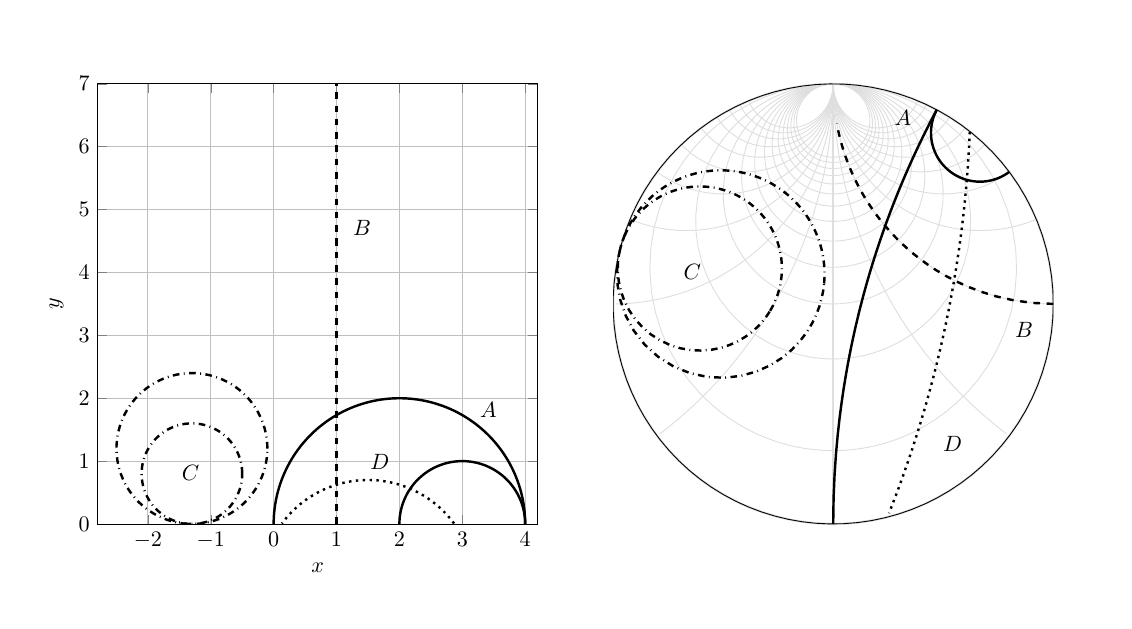
\begin{tikzpicture}[scale=0.8]

\begin{axis}[%
width=2.751in,
height=2.751in,
at={(0.437in,0.481in)},
scale only axis,
xmin=-2.8,
xmax=4.2,
ymin=0,
ymax=7,
xlabel=$x$,
ylabel=$y$,
axis background/.style={fill=white},
xmajorgrids,
ymajorgrids
]
\addplot [color=black, line width=1.1pt, forget plot]
  table[row sep=crcr]{%
4	0\\
3.99899308476637	0.0634558669961353\\
3.99597335294377	0.126847839313129\\
3.99094384514617	0.190112086608365\\
3.98390962566159	0.253184907147498\\
3.97487777735279	0.3160027919467\\
3.96385739452541	0.37850248872082\\
3.95085957377081	0.440621065573081\\
3.93589740279271	0.502295974362158\\
3.91898594722899	0.563465113682859\\
3.90014223548189	0.624066891396974\\
3.87938524157182	0.684040286651338\\
3.85673586603215	0.743324911320655\\
3.83221691486414	0.801861070813227\\
3.80585307657324	0.859589824178343\\
3.77767089730985	0.916453043454821\\
3.74769875413957	0.972393472200937\\
3.71596682646995	1.02735478314681\\
3.68250706566236	1.0812816349112\\
3.64735316285967	1.13411972772554\\
3.61054051506212	1.18581585810928\\
3.57210618948558	1.23631797244121\\
3.53208888623796	1.28557521937308\\
3.49052889935151	1.33353800103258\\
3.44746807621014	1.38015802296422\\
3.40294977541264	1.42538834275773\\
3.35701882311426	1.46918341731507\\
3.30972146789057	1.51149914870852\\
3.26110533416905	1.55229292858351\\
3.21121937427533	1.59152368106166\\
3.1601138191424	1.62915190410067\\
3.10784012773222	1.66513970926954\\
3.05445093522101	1.69945085989903\\
3	1.73205080756888\\
2.94454214954537	1.76290672689516\\
2.88813322521155	1.79198754858267\\
2.83083002600377	1.81926399070904\\
2.77269025138626	1.84470858820916\\
2.71377244318374	1.86829572053021\\
2.65413592663484	1.89000163742934\\
2.59384075065655	1.90980448288815\\
2.53294762738007	1.92768431711988\\
2.47151787101885	1.94362313664708\\
2.40961333613038	1.95760489242956\\
2.34729635533386	1.96961550602442\\
2.28462967654657	1.97964288376187\\
2.22167639980202	1.98767692892251\\
2.15849991371358	1.99370955190388\\
2.09516383164748	1.99773467836602\\
2.03173192766962	1.99974825534775\\
1.96826807233038	1.99974825534775\\
1.90483616835252	1.99773467836602\\
1.84150008628642	1.99370955190388\\
1.77832360019798	1.98767692892251\\
1.71537032345343	1.97964288376187\\
1.65270364466614	1.96961550602442\\
1.59038666386962	1.95760489242956\\
1.52848212898115	1.94362313664708\\
1.46705237261993	1.92768431711988\\
1.40615924934345	1.90980448288815\\
1.34586407336516	1.89000163742934\\
1.28622755681626	1.86829572053021\\
1.22730974861374	1.84470858820916\\
1.16916997399623	1.81926399070904\\
1.11186677478845	1.79198754858267\\
1.05545785045463	1.76290672689516\\
1	1.73205080756888\\
0.945549064778996	1.69945085989903\\
0.892159872267779	1.66513970926954\\
0.839886180857604	1.62915190410067\\
0.788780625724667	1.59152368106166\\
0.738894665830955	1.55229292858351\\
0.69027853210943	1.51149914870852\\
0.642981176885736	1.46918341731507\\
0.597050224587357	1.42538834275773\\
0.55253192378986	1.38015802296422\\
0.509471100648491	1.33353800103258\\
0.467911113762044	1.28557521937308\\
0.427893810514425	1.23631797244121\\
0.389459484937883	1.18581585810928\\
0.352646837140334	1.13411972772554\\
0.317492934337638	1.0812816349112\\
0.284033173530046	1.02735478314681\\
0.25230124586043	0.972393472200937\\
0.222329102690153	0.916453043454822\\
0.194146923426757	0.859589824178343\\
0.167783085135861	0.801861070813227\\
0.143264133967855	0.743324911320656\\
0.120614758428183	0.684040286651337\\
0.0998577645181093	0.624066891396975\\
0.0810140527710053	0.563465113682859\\
0.0641025972072875	0.502295974362159\\
0.0491404262291859	0.440621065573082\\
0.0361426054745866	0.37850248872082\\
0.0251222226472114	0.3160027919467\\
0.0160903743384093	0.253184907147499\\
0.00905615485383082	0.190112086608366\\
0.00402664705623135	0.12684783931313\\
0.00100691523362983	0.0634558669961353\\
0	2.44929359829471e-16\\
};
\addplot [color=black, line width=1.1pt, forget plot]
  table[row sep=crcr]{%
4	0\\
3.99949654238319	0.0317279334980676\\
3.99798667647188	0.0634239196565645\\
3.99547192257308	0.0950560433041827\\
3.9919548128308	0.126592453573749\\
3.98743888867639	0.15800139597335\\
3.98192869726271	0.18925124436041\\
3.97542978688541	0.220310532786541\\
3.96794870139636	0.251147987181079\\
3.9594929736145	0.28173255684143\\
3.95007111774095	0.312033445698487\\
3.93969262078591	0.342020143325669\\
3.92836793301607	0.371662455660328\\
3.91610845743207	0.400930535406614\\
3.90292653828662	0.429794912089172\\
3.88883544865492	0.45822652172741\\
3.87384937706979	0.486196736100469\\
3.85798341323498	0.513677391573406\\
3.84125353283118	0.540640817455598\\
3.82367658142983	0.567059863862771\\
3.80527025753106	0.592907929054641\\
3.78605309474279	0.618158986220605\\
3.76604444311898	0.642787609686539\\
3.74526444967576	0.666769000516292\\
3.72373403810507	0.690079011482112\\
3.70147488770632	0.712694171378863\\
3.67850941155713	0.734591708657533\\
3.65486073394529	0.755749574354258\\
3.63055266708452	0.776146464291757\\
3.60560968713767	0.795761840530832\\
3.5800569095712	0.814575952050336\\
3.55392006386611	0.832569854634771\\
3.5272254676105	0.849725429949514\\
3.5	0.866025403784439\\
3.47227107477268	0.881453363447582\\
3.44406661260577	0.895993774291336\\
3.41541501300189	0.909631995354518\\
3.38634512569313	0.922354294104581\\
3.35688622159187	0.934147860265107\\
3.32706796331742	0.945000818714668\\
3.29692037532827	0.954902241444074\\
3.26647381369004	0.963842158559942\\
3.23575893550943	0.971811568323542\\
3.20480666806519	0.978802446214779\\
3.17364817766693	0.984807753012208\\
3.14231483827329	0.989821441880933\\
3.11083819990101	0.993838464461254\\
3.07924995685679	0.996854775951942\\
3.04758191582374	0.998867339183008\\
3.01586596383481	0.999874127673875\\
2.98413403616519	0.999874127673875\\
2.95241808417626	0.998867339183008\\
2.92075004314321	0.996854775951942\\
2.88916180009899	0.993838464461254\\
2.85768516172672	0.989821441880933\\
2.82635182233307	0.984807753012208\\
2.79519333193481	0.978802446214779\\
2.76424106449057	0.971811568323542\\
2.73352618630997	0.963842158559942\\
2.70307962467173	0.954902241444074\\
2.67293203668258	0.945000818714668\\
2.64311377840813	0.934147860265107\\
2.61365487430687	0.922354294104581\\
2.58458498699811	0.909631995354518\\
2.55593338739423	0.895993774291336\\
2.52772892522732	0.881453363447582\\
2.5	0.866025403784439\\
2.4727745323895	0.849725429949515\\
2.44607993613389	0.832569854634771\\
2.4199430904288	0.814575952050336\\
2.39439031286233	0.795761840530832\\
2.36944733291548	0.776146464291757\\
2.34513926605471	0.755749574354258\\
2.32149058844287	0.734591708657533\\
2.29852511229368	0.712694171378863\\
2.27626596189493	0.690079011482112\\
2.25473555032425	0.666769000516292\\
2.23395555688102	0.642787609686539\\
2.21394690525721	0.618158986220605\\
2.19472974246894	0.59290792905464\\
2.17632341857017	0.56705986386277\\
2.15874646716882	0.540640817455598\\
2.14201658676502	0.513677391573407\\
2.12615062293021	0.486196736100469\\
2.11116455134508	0.458226521727411\\
2.09707346171338	0.429794912089171\\
2.08389154256793	0.400930535406614\\
2.07163206698393	0.371662455660328\\
2.06030737921409	0.342020143325668\\
2.04992888225905	0.312033445698487\\
2.0405070263855	0.28173255684143\\
2.03205129860364	0.251147987181079\\
2.02457021311459	0.220310532786541\\
2.01807130273729	0.18925124436041\\
2.01256111132361	0.15800139597335\\
2.0080451871692	0.126592453573749\\
2.00452807742692	0.0950560433041829\\
2.00201332352812	0.0634239196565648\\
2.00050345761681	0.0317279334980677\\
2	1.22464679914735e-16\\
};
\addplot [color=black, dashed, line width=1.1pt, forget plot]
  table[row sep=crcr]{%
1	0\\
1	0.101010101010101\\
1	0.202020202020202\\
1	0.303030303030303\\
1	0.404040404040404\\
1	0.505050505050505\\
1	0.606060606060606\\
1	0.707070707070707\\
1	0.808080808080808\\
1	0.909090909090909\\
1	1.01010101010101\\
1	1.11111111111111\\
1	1.21212121212121\\
1	1.31313131313131\\
1	1.41414141414141\\
1	1.51515151515152\\
1	1.61616161616162\\
1	1.71717171717172\\
1	1.81818181818182\\
1	1.91919191919192\\
1	2.02020202020202\\
1	2.12121212121212\\
1	2.22222222222222\\
1	2.32323232323232\\
1	2.42424242424242\\
1	2.52525252525253\\
1	2.62626262626263\\
1	2.72727272727273\\
1	2.82828282828283\\
1	2.92929292929293\\
1	3.03030303030303\\
1	3.13131313131313\\
1	3.23232323232323\\
1	3.33333333333333\\
1	3.43434343434343\\
1	3.53535353535354\\
1	3.63636363636364\\
1	3.73737373737374\\
1	3.83838383838384\\
1	3.93939393939394\\
1	4.04040404040404\\
1	4.14141414141414\\
1	4.24242424242424\\
1	4.34343434343434\\
1	4.44444444444444\\
1	4.54545454545455\\
1	4.64646464646465\\
1	4.74747474747475\\
1	4.84848484848485\\
1	4.94949494949495\\
1	5.05050505050505\\
1	5.15151515151515\\
1	5.25252525252525\\
1	5.35353535353535\\
1	5.45454545454545\\
1	5.55555555555556\\
1	5.65656565656566\\
1	5.75757575757576\\
1	5.85858585858586\\
1	5.95959595959596\\
1	6.06060606060606\\
1	6.16161616161616\\
1	6.26262626262626\\
1	6.36363636363636\\
1	6.46464646464646\\
1	6.56565656565657\\
1	6.66666666666667\\
1	6.76767676767677\\
1	6.86868686868687\\
1	6.96969696969697\\
1	7.07070707070707\\
1	7.17171717171717\\
1	7.27272727272727\\
1	7.37373737373737\\
1	7.47474747474747\\
1	7.57575757575758\\
1	7.67676767676768\\
1	7.77777777777778\\
1	7.87878787878788\\
1	7.97979797979798\\
1	8.08080808080808\\
1	8.18181818181818\\
1	8.28282828282828\\
1	8.38383838383838\\
1	8.48484848484848\\
1	8.58585858585859\\
1	8.68686868686869\\
1	8.78787878787879\\
1	8.88888888888889\\
1	8.98989898989899\\
1	9.09090909090909\\
1	9.19191919191919\\
1	9.29292929292929\\
1	9.39393939393939\\
1	9.49494949494949\\
1	9.5959595959596\\
1	9.6969696969697\\
1	9.7979797979798\\
1	9.8989898989899\\
1	10\\
};
\addplot [color=black, dashdotted, line width=1.1pt, forget plot]
  table[row sep=crcr]{%
-0.1	1.2\\
-0.102415988233739	1.27610870358788\\
-0.109654224603046	1.3519109442885\\
-0.121685563284752	1.42710149323249\\
-0.138461558324373	1.50137758461729\\
-0.159914658710866	1.57444013483818\\
-0.185958480380713	1.64599494679239\\
-0.216488154056055	1.71575389450701\\
-0.251380747516258	1.78343608332056\\
-0.290495760602583	1.84876898094672\\
-0.33367569096273	1.91148951486557\\
-0.380746668257226	1.97134513162385\\
-0.431519154273916	2.02809481377853\\
-0.485788706131441	2.08151005038904\\
-0.543336799498573	2.13137575715011\\
-0.603931708514562	2.1774911424604\\
-0.667329438867397	2.21967051593942\\
-0.733274710272781	2.2577440361371\\
-0.801501984397736	2.29155839442542\\
-0.871736534089754	2.32097743231813\\
-0.94369554960607	2.34588268973289\\
-1.01708927738869	2.36617388198825\\
-1.09162218679968	2.38176930361465\\
-1.16699416011879	2.39260615735351\\
-1.24290170101151	2.39864080701961\\
-1.31903915660177	2.39984895320865\\
-1.39509994822815	2.39622573114233\\
-1.47077780592794	2.38778573025712\\
-1.54576800167823	2.37456293545773\\
-1.61976857642804	2.35661059027193\\
-1.69248155598091	2.3340009824576\\
-1.76361415083175	2.3068251529255\\
-1.83287993512693	2.2751925291496\\
-1.9	2.23923048454133\\
-1.96470407663933	2.19908382556173\\
-2.0267316245652	2.154914208637\\
-2.08583288073434	2.10689948922511\\
-2.14176986524759	2.05523300565464\\
-2.19431733961091	2.00012280061955\\
-2.24326371369134	1.94179078346473\\
-2.2884118977158	1.88047183663532\\
-2.32958009588197	1.81641286988809\\
-2.36660253838591	1.74987182607289\\
-2.39933014891848	1.68111664248794\\
-2.42763114494309	1.6104241719908\\
-2.4513915683374	1.53807906820972\\
-2.47051574426249	1.46437263934385\\
-2.48492666641167	1.38960167516802\\
-2.4945663070877	1.31406725196502\\
-2.49939585085982	1.23807352019768\\
-2.49939585085982	1.16192647980232\\
-2.4945663070877	1.08593274803498\\
-2.48492666641167	1.01039832483198\\
-2.47051574426249	0.935627360656151\\
-2.4513915683374	0.861920931790285\\
-2.42763114494309	0.789575828009198\\
-2.39933014891848	0.718883357512064\\
-2.36660253838591	0.650128173927107\\
-2.32958009588197	0.583587130111913\\
-2.2884118977158	0.519528163364676\\
-2.24326371369134	0.458209216535274\\
-2.19431733961091	0.39987719938045\\
-2.14176986524759	0.344766994345365\\
-2.08583288073434	0.29310051077489\\
-2.0267316245652	0.245085791363002\\
-1.96470407663933	0.200916174438274\\
-1.9	0.160769515458673\\
-1.83287993512693	0.124807470850397\\
-1.76361415083175	0.0931748470745024\\
-1.69248155598091	0.0659990175423979\\
-1.61976857642804	0.0433894097280696\\
-1.54576800167823	0.0254370645422655\\
-1.47077780592794	0.0122142697428809\\
-1.39509994822815	0.00377426885766918\\
-1.31903915660177	0.000151046791349918\\
-1.24290170101151	0.00135919298039044\\
-1.16699416011879	0.00739384264649501\\
-1.09162218679968	0.0182306963853502\\
-1.01708927738869	0.0338261180117498\\
-0.94369554960607	0.0541173102671113\\
-0.871736534089753	0.0790225676818723\\
-0.801501984397737	0.108441605574578\\
-0.733274710272782	0.142255963862901\\
-0.667329438867397	0.180329484060583\\
-0.603931708514563	0.222508857539596\\
-0.543336799498573	0.268624242849892\\
-0.485788706131441	0.31848994961096\\
-0.431519154273917	0.371905186221465\\
-0.380746668257226	0.428654868376153\\
-0.33367569096273	0.488510485134431\\
-0.290495760602583	0.551231019053283\\
-0.251380747516258	0.616563916679437\\
-0.216488154056055	0.684246105492994\\
-0.185958480380713	0.754005053207607\\
-0.159914658710866	0.825559865161815\\
-0.138461558324373	0.898622415382705\\
-0.121685563284752	0.972898506767507\\
-0.109654224603046	1.0480890557115\\
-0.102415988233739	1.12389129641212\\
-0.1	1.2\\
};
\addplot [color=black, dashdotted, line width=1.1pt, forget plot]
  table[row sep=crcr]{%
-0.5	0.8\\
-0.501610658822492	0.850739135725252\\
-0.506436149735364	0.901273962858999\\
-0.514457042189835	0.951400995488328\\
-0.525641038882915	1.00091838974486\\
-0.539943105807244	1.04962675655879\\
-0.557305653587142	1.09732996452826\\
-0.577658769370703	1.14383592967134\\
-0.600920498344172	1.18895738888037\\
-0.626997173735055	1.23251265396448\\
-0.655783793975153	1.27432634324371\\
-0.687164445504818	1.31423008774923\\
-0.721012769515944	1.35206320918569\\
-0.757192470754294	1.38767336692603\\
-0.795557866332382	1.42091717143341\\
-0.835954472343041	1.45166076164027\\
-0.878219625911598	1.47978034395961\\
-0.922183140181854	1.50516269075807\\
-0.967667989598491	1.52770559628361\\
-1.0144910227265	1.54731828821209\\
-1.06246369973738	1.56392179315526\\
-1.11139285159246	1.57744925465883\\
-1.16108145786646	1.58784620240977\\
-1.21132944007919	1.595070771569\\
-1.26193446734101	1.59909387134641\\
-1.31269277106785	1.5998993021391\\
-1.36339996548543	1.59748382076155\\
-1.41385187061863	1.59185715350475\\
-1.46384533445215	1.58304195697182\\
-1.51317905095203	1.57107372684795\\
-1.56165437065394	1.55600065497173\\
-1.6090761005545	1.53788343528367\\
-1.65525329008462	1.51679501943307\\
-1.7	1.49282032302755\\
-1.74313605109289	1.46605588370782\\
-1.78448774971013	1.43660947242467\\
-1.82388858715623	1.40459965948341\\
-1.86117991016506	1.37015533710309\\
-1.8962115597406	1.33341520041303\\
-1.92884247579423	1.29452718897648\\
-1.95894126514387	1.25364789109022\\
-1.98638673058798	1.21094191325873\\
-2.01106835892394	1.16658121738193\\
-2.03288676594566	1.12074442832529\\
-2.05175409662873	1.07361611466053\\
-2.0675943788916	1.02538604547314\\
-2.08034382950833	0.976248426229233\\
-2.08995111094112	0.92640111677868\\
-2.09637753805847	0.876044834643346\\
-2.09959723390655	0.825382346798454\\
-2.09959723390655	0.774617653201547\\
-2.09637753805847	0.723955165356654\\
-2.08995111094112	0.67359888322132\\
-2.08034382950833	0.623751573770768\\
-2.0675943788916	0.574613954526856\\
-2.05175409662873	0.526383885339465\\
-2.03288676594566	0.479255571674709\\
-2.01106835892394	0.433418782618071\\
-1.98638673058798	0.389058086741275\\
-1.95894126514387	0.346352108909784\\
-1.92884247579423	0.305472811023516\\
-1.8962115597406	0.266584799586967\\
-1.86117991016506	0.22984466289691\\
-1.82388858715623	0.195400340516593\\
-1.78448774971013	0.163390527575335\\
-1.74313605109289	0.133944116292183\\
-1.7	0.107179676972449\\
-1.65525329008462	0.0832049805669316\\
-1.6090761005545	0.0621165647163349\\
-1.56165437065394	0.0439993450282653\\
-1.51317905095203	0.0289262731520464\\
-1.46384533445215	0.0169580430281771\\
-1.41385187061863	0.00814284649525387\\
-1.36339996548543	0.00251617923844616\\
-1.31269277106785	0.000100697860899945\\
-1.26193446734101	0.00090612865359363\\
-1.21132944007919	0.00492922843099675\\
-1.16108145786646	0.0121537975902335\\
-1.11139285159246	0.0225507453411665\\
-1.06246369973738	0.0360782068447409\\
-1.0144910227265	0.0526817117879148\\
-0.967667989598491	0.0722944037163852\\
-0.922183140181854	0.0948373092419341\\
-0.878219625911598	0.120219656040389\\
-0.835954472343042	0.148339238359731\\
-0.795557866332382	0.179082828566595\\
-0.757192470754294	0.212326633073974\\
-0.721012769515945	0.24793679081431\\
-0.687164445504817	0.285769912250769\\
-0.655783793975153	0.325673656756287\\
-0.626997173735055	0.367487346035522\\
-0.600920498344172	0.411042611119625\\
-0.577658769370703	0.456164070328662\\
-0.557305653587142	0.502670035471738\\
-0.539943105807244	0.55037324344121\\
-0.525641038882915	0.599081610255137\\
-0.514457042189835	0.648599004511672\\
-0.506436149735364	0.698726037141\\
-0.501610658822492	0.749260864274748\\
-0.5	0.8\\
};
\addplot [color=black, dotted, line width=1.1pt, forget plot]
  table[row sep=crcr]{%
2.8689594378028	0.00794347939288875\\
2.83629026106274	0.0508702765750286\\
2.80227555330226	0.092738936467117\\
2.76694956444878	0.133507300877696\\
2.73034786477862	0.17313431951959\\
2.69250730910075	0.211580091344067\\
2.65346599964712	0.248805904717807\\
2.61326324770698	0.284774276402239\\
2.57193953404369	0.319448989295987\\
2.52953646813403	0.352795128902414\\
2.48609674627104	0.384779118485571\\
2.44166410857239	0.415368752879111\\
2.39628329493785	0.444533230914174\\
2.35	0.472243186433546\\
2.30286082711356	0.49847071786089\\
2.25491324142982	0.523189416295271\\
2.20620552210321	0.546374392102681\\
2.15678671367832	0.568002299977789\\
2.10670657670618	0.588051362450681\\
2.05601553763962	0.606501391814936\\
2.00476463805807	0.623333810454926\\
1.95300548327306	0.638531669551901\\
1.90079019036603	0.652079666150021\\
1.84817133571082	0.663964158565124\\
1.79520190203378	0.674173180120754\\
1.74193522506458	0.682696451197585\\
1.68842493983172	0.689525389584132\\
1.63472492665654	0.694653119118302\\
1.58088925690036	0.698074476611114\\
1.52697213851917	0.699786017045588\\
1.47302786148083	0.699786017045588\\
1.41911074309964	0.698074476611114\\
1.36527507334346	0.694653119118302\\
1.31157506016828	0.689525389584132\\
1.25806477493542	0.682696451197586\\
1.20479809796622	0.674173180120754\\
1.15182866428918	0.663964158565124\\
1.09920980963397	0.652079666150021\\
1.04699451672694	0.638531669551902\\
0.995235361941933	0.623333810454926\\
0.943984462360383	0.606501391814936\\
0.893293423293818	0.588051362450682\\
0.843213286321681	0.568002299977788\\
0.793794477896793	0.546374392102681\\
0.745086758570185	0.523189416295271\\
0.69713917288644	0.49847071786089\\
0.65	0.472243186433546\\
0.603716705062146	0.444533230914175\\
0.558335891427613	0.415368752879111\\
0.513903253728963	0.384779118485571\\
0.470463531865967	0.352795128902415\\
0.428060465956312	0.319448989295987\\
0.386736752293016	0.284774276402239\\
0.346534000352875	0.248805904717807\\
0.307492690899254	0.211580091344067\\
0.269652135221381	0.17313431951959\\
0.233050435551217	0.133507300877696\\
0.197724446697738	0.0927389364671172\\
0.163709738937262	0.0508702765750293\\
0.1310405621972	0.00794347939288875\\
};
\end{axis}

\begin{axis}[%
width=2.751in,
height=3.163in,
at={(3.659in,0.275in)},
scale only axis,
xmin=-1,
xmax=1,
ymin=-1.15,
ymax=1.15,
axis line style={draw=none},
ticks=none,
axis x line*=bottom,
axis y line*=left
]

\addplot[area legend, draw=white!83!darkgray, fill=white, forget plot]
table[row sep=crcr] {%
x	y\\
1	0\\
0.998026728428272	0.0627905195293134\\
0.992114701314478	0.125333233564304\\
0.982287250728689	0.187381314585725\\
0.968583161128631	0.248689887164855\\
0.951056516295154	0.309016994374947\\
0.929776485888251	0.368124552684678\\
0.904827052466019	0.425779291565073\\
0.876306680043864	0.481753674101715\\
0.844327925502015	0.535826794978997\\
0.809016994374947	0.587785252292473\\
0.770513242775789	0.63742398974869\\
0.728968627421412	0.684547105928689\\
0.684547105928689	0.728968627421412\\
0.63742398974869	0.770513242775789\\
0.587785252292473	0.809016994374947\\
0.535826794978997	0.844327925502015\\
0.481753674101715	0.876306680043864\\
0.425779291565073	0.90482705246602\\
0.368124552684678	0.929776485888251\\
0.309016994374947	0.951056516295154\\
0.248689887164855	0.968583161128631\\
0.187381314585725	0.982287250728689\\
0.125333233564304	0.992114701314478\\
0.0627905195293133	0.998026728428272\\
0	1\\
-0.0627905195293134	0.998026728428272\\
-0.125333233564304	0.992114701314478\\
-0.187381314585725	0.982287250728689\\
-0.248689887164855	0.968583161128631\\
-0.309016994374948	0.951056516295154\\
-0.368124552684678	0.929776485888251\\
-0.425779291565073	0.904827052466019\\
-0.481753674101715	0.876306680043863\\
-0.535826794978997	0.844327925502015\\
-0.587785252292473	0.809016994374947\\
-0.63742398974869	0.770513242775789\\
-0.684547105928689	0.728968627421411\\
-0.728968627421412	0.684547105928689\\
-0.770513242775789	0.63742398974869\\
-0.809016994374947	0.587785252292473\\
-0.844327925502015	0.535826794978997\\
-0.876306680043864	0.481753674101715\\
-0.90482705246602	0.425779291565072\\
-0.929776485888251	0.368124552684678\\
-0.951056516295154	0.309016994374947\\
-0.968583161128631	0.248689887164855\\
-0.982287250728689	0.187381314585725\\
-0.992114701314478	0.125333233564304\\
-0.998026728428272	0.0627905195293131\\
-1	0\\
-0.998026728428272	-0.0627905195293129\\
-0.992114701314478	-0.125333233564304\\
-0.982287250728689	-0.187381314585724\\
-0.968583161128631	-0.248689887164855\\
-0.951056516295154	-0.309016994374947\\
-0.929776485888252	-0.368124552684677\\
-0.90482705246602	-0.425779291565072\\
-0.876306680043864	-0.481753674101715\\
-0.844327925502015	-0.535826794978996\\
-0.809016994374947	-0.587785252292473\\
-0.77051324277579	-0.637423989748689\\
-0.728968627421412	-0.684547105928688\\
-0.684547105928689	-0.728968627421411\\
-0.63742398974869	-0.770513242775789\\
-0.587785252292473	-0.809016994374947\\
-0.535826794978997	-0.844327925502015\\
-0.481753674101716	-0.876306680043863\\
-0.425779291565073	-0.904827052466019\\
-0.368124552684678	-0.929776485888251\\
-0.309016994374948	-0.951056516295154\\
-0.248689887164855	-0.968583161128631\\
-0.187381314585725	-0.982287250728688\\
-0.125333233564305	-0.992114701314478\\
-0.0627905195293132	-0.998026728428272\\
0	-1\\
0.0627905195293128	-0.998026728428272\\
0.125333233564304	-0.992114701314478\\
0.187381314585724	-0.982287250728689\\
0.248689887164855	-0.968583161128631\\
0.309016994374947	-0.951056516295154\\
0.368124552684677	-0.929776485888252\\
0.425779291565073	-0.90482705246602\\
0.481753674101715	-0.876306680043864\\
0.535826794978997	-0.844327925502015\\
0.587785252292473	-0.809016994374948\\
0.637423989748689	-0.77051324277579\\
0.684547105928689	-0.728968627421412\\
0.728968627421411	-0.684547105928689\\
0.770513242775789	-0.63742398974869\\
0.809016994374947	-0.587785252292473\\
0.844327925502015	-0.535826794978997\\
0.876306680043864	-0.481753674101715\\
0.904827052466019	-0.425779291565073\\
0.929776485888251	-0.368124552684678\\
0.951056516295154	-0.309016994374948\\
0.968583161128631	-0.248689887164855\\
0.982287250728689	-0.187381314585725\\
0.992114701314478	-0.125333233564305\\
0.998026728428272	-0.0627905195293133\\
1	0\\
}--cycle;
\addplot [color=white!83!darkgray, line width=1.0pt, forget plot]
  table[row sep=crcr]{%
1	0\\
0.998026728428272	0.0627905195293134\\
0.992114701314478	0.125333233564304\\
0.982287250728689	0.187381314585725\\
0.968583161128631	0.248689887164855\\
0.951056516295154	0.309016994374947\\
0.929776485888251	0.368124552684678\\
0.904827052466019	0.425779291565073\\
0.876306680043864	0.481753674101715\\
0.844327925502015	0.535826794978997\\
0.809016994374947	0.587785252292473\\
0.770513242775789	0.63742398974869\\
0.728968627421412	0.684547105928689\\
0.684547105928689	0.728968627421412\\
0.63742398974869	0.770513242775789\\
0.587785252292473	0.809016994374947\\
0.535826794978997	0.844327925502015\\
0.481753674101715	0.876306680043864\\
0.425779291565073	0.90482705246602\\
0.368124552684678	0.929776485888251\\
0.309016994374947	0.951056516295154\\
0.248689887164855	0.968583161128631\\
0.187381314585725	0.982287250728689\\
0.125333233564304	0.992114701314478\\
0.0627905195293133	0.998026728428272\\
0	1\\
-0.0627905195293134	0.998026728428272\\
-0.125333233564304	0.992114701314478\\
-0.187381314585725	0.982287250728689\\
-0.248689887164855	0.968583161128631\\
-0.309016994374948	0.951056516295154\\
-0.368124552684678	0.929776485888251\\
-0.425779291565073	0.904827052466019\\
-0.481753674101715	0.876306680043863\\
-0.535826794978997	0.844327925502015\\
-0.587785252292473	0.809016994374947\\
-0.63742398974869	0.770513242775789\\
-0.684547105928689	0.728968627421411\\
-0.728968627421412	0.684547105928689\\
-0.770513242775789	0.63742398974869\\
-0.809016994374947	0.587785252292473\\
-0.844327925502015	0.535826794978997\\
-0.876306680043864	0.481753674101715\\
-0.90482705246602	0.425779291565072\\
-0.929776485888251	0.368124552684678\\
-0.951056516295154	0.309016994374947\\
-0.968583161128631	0.248689887164855\\
-0.982287250728689	0.187381314585725\\
-0.992114701314478	0.125333233564304\\
-0.998026728428272	0.0627905195293131\\
-1	0\\
-0.998026728428272	-0.0627905195293129\\
-0.992114701314478	-0.125333233564304\\
-0.982287250728689	-0.187381314585724\\
-0.968583161128631	-0.248689887164855\\
-0.951056516295154	-0.309016994374947\\
-0.929776485888252	-0.368124552684677\\
-0.90482705246602	-0.425779291565072\\
-0.876306680043864	-0.481753674101715\\
-0.844327925502015	-0.535826794978996\\
-0.809016994374947	-0.587785252292473\\
-0.77051324277579	-0.637423989748689\\
-0.728968627421412	-0.684547105928688\\
-0.684547105928689	-0.728968627421411\\
-0.63742398974869	-0.770513242775789\\
-0.587785252292473	-0.809016994374947\\
-0.535826794978997	-0.844327925502015\\
-0.481753674101716	-0.876306680043863\\
-0.425779291565073	-0.904827052466019\\
-0.368124552684678	-0.929776485888251\\
-0.309016994374948	-0.951056516295154\\
-0.248689887164855	-0.968583161128631\\
-0.187381314585725	-0.982287250728688\\
-0.125333233564305	-0.992114701314478\\
-0.0627905195293132	-0.998026728428272\\
0	-1\\
0.0627905195293128	-0.998026728428272\\
0.125333233564304	-0.992114701314478\\
0.187381314585724	-0.982287250728689\\
0.248689887164855	-0.968583161128631\\
0.309016994374947	-0.951056516295154\\
0.368124552684677	-0.929776485888252\\
0.425779291565073	-0.90482705246602\\
0.481753674101715	-0.876306680043864\\
0.535826794978997	-0.844327925502015\\
0.587785252292473	-0.809016994374948\\
0.637423989748689	-0.77051324277579\\
0.684547105928689	-0.728968627421412\\
0.728968627421411	-0.684547105928689\\
0.770513242775789	-0.63742398974869\\
0.809016994374947	-0.587785252292473\\
0.844327925502015	-0.535826794978997\\
0.876306680043864	-0.481753674101715\\
0.904827052466019	-0.425779291565073\\
0.929776485888251	-0.368124552684678\\
0.951056516295154	-0.309016994374948\\
0.968583161128631	-0.248689887164855\\
0.982287250728689	-0.187381314585725\\
0.992114701314478	-0.125333233564305\\
0.998026728428272	-0.0627905195293133\\
1	0\\
};
\addplot [color=white!83!darkgray, line width=1.0pt, forget plot]
  table[row sep=crcr]{%
-6.12323399573677e-17	-1\\
6.12323399573677e-17	1\\
};
\addplot [color=mycolor1, forget plot]
  table[row sep=crcr]{%
-0.00199999712000435	0.999997600003456\\
-0.00224664398363806	0.999996971548983\\
-0.00252370797955442	0.999996178530058\\
-0.00283494012353416	0.999995177854746\\
-0.003184553960115	0.99999391514743\\
-0.00357728257777211	0.999992321794242\\
-0.00401844264469811	0.999990311214903\\
-0.0045140063265093	0.999987774158448\\
-0.00507068205155084	0.99998457276732\\
-0.00569600520591349	0.99998053308744\\
-0.0063984399699689	0.999975435617525\\
-0.00718749365233697	0.999969003384525\\
-0.00807384503687127	0.999960886897892\\
-0.00906948843444717	0.999950645166183\\
-0.0101878953248085	0.999937721746162\\
-0.0114441956847285	0.999921414525672\\
-0.0128553813268	0.999900837602657\\
-0.0144405338166638	0.999874873195823\\
-0.0162210797920176	0.999842110984864\\
-0.0182210767683516	0.999800771601668\\
-0.0204675327741759	0.999748610143167\\
-0.0229907633971465	0.999682794507455\\
-0.0258247900184589	0.999599752013231\\
-0.0290077831310961	0.999494976081196\\
-0.0325825546263726	0.999362782652843\\
-0.0365971027176137	0.999196003397284\\
-0.0411052126413894	0.998985599491188\\
-0.0461671152804215	0.998720175709882\\
-0.0518502041675389	0.998385369577831\\
-0.0582298086453487	0.997963084215528\\
-0.0653900168343093	0.997430526101376\\
-0.0734245358935307	0.99675900006896\\
-0.082437568002336	0.995912403361348\\
-0.0925446673960414	0.99484534846245\\
-0.103873525104518	0.993500830950416\\
-0.116564601709243	0.991807344413686\\
-0.130771491790237	0.98967533088558\\
-0.146660853447061	0.986992844787677\\
-0.16441166839423	0.983620305339187\\
-0.184213508358292	0.979384223867675\\
-0.206263367957457	0.974069829580518\\
-0.23076048103551	0.967412596932132\\
-0.257898369649207	0.959088823964609\\
-0.287853195848177	0.948705656797233\\
-0.320767327769218	0.935791341787833\\
-0.356726955549251	0.919787057858545\\
-0.395732706670743	0.900042470273175\\
-0.437662681288327	0.87581814685405\\
-0.482228383431657	0.846299089861245\\
-0.528925920084236	0.810624596587161\\
-0.576987762463246	0.76793995429227\\
-0.625344224807978	0.717474296373948\\
-0.672607950226452	0.658645314309646\\
-0.717097554226676	0.591184678259302\\
-0.756915717850875	0.515268216454872\\
-0.790089790721782	0.431624336949405\\
-0.814768176075881	0.341587402139701\\
-0.829445879423595	0.247065532029702\\
-0.833174717646663	0.15040830516104\\
-0.825707398983585	0.0541867319751541\\
-0.807536529576367	-0.0390739414888499\\
-0.77981749168518	-0.127151515388628\\
-0.744196846366182	-0.208320664190088\\
-0.70259128704055	-0.281451540750917\\
-0.656967657329356	-0.346010562852671\\
-0.609163350863714	-0.401984769987578\\
-0.560766818139393	-0.449762583221969\\
-0.513059158826349	-0.490002766144732\\
-0.467005474047291	-0.523514709244267\\
-0.423279809725554	-0.551162454450012\\
-0.382308222238019	-0.573795937151818\\
-0.344318019516608	-0.592207200244433\\
-0.309385397156337	-0.607106633771427\\
-0.277477273508218	-0.619113714311944\\
-0.248485696437548	-0.628757310285494\\
-0.222254781135673	-0.636481673745476\\
-0.198600969213317	-0.642655333202345\\
-0.177327727931079	-0.64758103603273\\
-0.1582358433023	-0.65150560268671\\
-0.141130347656796	-0.65462905925349\\
-0.125824951645447	-0.65711274918922\\
-0.112144672982432	-0.65908633318626\\
-0.0999271938546907	-0.660653706811934\\
-0.0890233449863217	-0.661897928577356\\
-0.0792970078031139	-0.662885278058869\\
-0.0706246441907855	-0.663668569293707\\
-0.0628946018331757	-0.664289838515579\\
-0.0560062978203572	-0.664782513409243\\
-0.0498693503703662	-0.665173157060283\\
-0.0444027050068869	-0.665482865708685\\
-0.0395337849284048	-0.665728386354241\\
-0.0351976837159402	-0.665923008686972\\
-0.031336410550455	-0.666077275862042\\
-0.0278981927102469	-0.666199550254122\\
-0.0248368365372602	-0.66629646336687\\
-0.0221111457537746	-0.66637327335896\\
-0.019684394586814	-0.666434148993836\\
-0.0175238523392119	-0.666482395052566\\
-0.015600355637463	-0.666520631213245\\
-0.0138879244496911	-0.666550933962919\\
0.013887924449691	-0.666550933962919\\
0.0156003556374629	-0.666520631213245\\
0.0175238523392118	-0.666482395052566\\
0.019684394586814	-0.666434148993836\\
0.0221111457537745	-0.66637327335896\\
0.0248368365372601	-0.66629646336687\\
0.0278981927102468	-0.666199550254122\\
0.031336410550455	-0.666077275862042\\
0.0351976837159402	-0.665923008686972\\
0.0395337849284047	-0.665728386354241\\
0.0444027050068868	-0.665482865708685\\
0.0498693503703662	-0.665173157060283\\
0.0560062978203572	-0.664782513409243\\
0.0628946018331757	-0.664289838515579\\
0.0706246441907854	-0.663668569293707\\
0.0792970078031138	-0.662885278058869\\
0.0890233449863216	-0.661897928577356\\
0.0999271938546906	-0.660653706811934\\
0.112144672982432	-0.65908633318626\\
0.125824951645447	-0.65711274918922\\
0.141130347656796	-0.65462905925349\\
0.1582358433023	-0.65150560268671\\
0.177327727931079	-0.64758103603273\\
0.198600969213317	-0.642655333202345\\
0.222254781135673	-0.636481673745476\\
0.248485696437548	-0.628757310285494\\
0.277477273508218	-0.619113714311944\\
0.309385397156337	-0.607106633771427\\
0.344318019516608	-0.592207200244433\\
0.382308222238019	-0.573795937151818\\
0.423279809725554	-0.551162454450012\\
0.467005474047291	-0.523514709244267\\
0.513059158826349	-0.490002766144732\\
0.560766818139393	-0.449762583221969\\
0.609163350863714	-0.401984769987578\\
0.656967657329356	-0.346010562852671\\
0.70259128704055	-0.281451540750917\\
0.744196846366182	-0.208320664190088\\
0.77981749168518	-0.127151515388628\\
0.807536529576367	-0.0390739414888499\\
0.825707398983585	0.0541867319751542\\
0.833174717646663	0.15040830516104\\
0.829445879423595	0.247065532029702\\
0.814768176075881	0.3415874021397\\
0.790089790721781	0.431624336949405\\
0.756915717850876	0.515268216454872\\
0.717097554226676	0.591184678259302\\
0.672607950226452	0.658645314309646\\
0.625344224807978	0.717474296373948\\
0.576987762463246	0.76793995429227\\
0.528925920084237	0.810624596587161\\
0.482228383431657	0.846299089861245\\
0.437662681288327	0.87581814685405\\
0.395732706670743	0.900042470273175\\
0.356726955549251	0.919787057858545\\
0.320767327769218	0.935791341787833\\
0.287853195848177	0.948705656797233\\
0.257898369649207	0.959088823964609\\
0.230760481035509	0.967412596932132\\
0.206263367957457	0.974069829580518\\
0.184213508358292	0.979384223867675\\
0.16441166839423	0.983620305339187\\
0.146660853447061	0.986992844787677\\
0.130771491790237	0.98967533088558\\
0.116564601709243	0.991807344413686\\
0.103873525104518	0.993500830950416\\
0.0925446673960413	0.99484534846245\\
0.0824375680023359	0.995912403361348\\
0.0734245358935306	0.99675900006896\\
0.0653900168343092	0.997430526101376\\
0.0582298086453486	0.997963084215528\\
0.0518502041675388	0.998385369577831\\
0.0461671152804214	0.998720175709882\\
0.0411052126413893	0.998985599491188\\
0.0365971027176136	0.999196003397284\\
0.0325825546263725	0.999362782652843\\
0.029007783131096	0.999494976081196\\
0.0258247900184588	0.999599752013231\\
0.0229907633971464	0.999682794507455\\
0.0204675327741758	0.999748610143167\\
0.0182210767683515	0.999800771601668\\
0.0162210797920175	0.999842110984864\\
0.0144405338166637	0.999874873195823\\
0.0128553813267999	0.999900837602657\\
0.0114441956847284	0.999921414525672\\
0.0101878953248084	0.999937721746162\\
0.00906948843444707	0.999950645166183\\
0.00807384503687117	0.999960886897892\\
0.00718749365233688	0.999969003384525\\
0.00639843996996881	0.999975435617525\\
0.00569600520591339	0.99998053308744\\
0.00507068205155074	0.99998457276732\\
0.0045140063265092	0.999987774158448\\
0.00401844264469801	0.999990311214903\\
0.00357728257777201	0.999992321794242\\
0.0031845539601149	0.99999391514743\\
0.00283494012353406	0.999995177854746\\
0.00252370797955432	0.999996178530058\\
0.00224664398363797	0.999996971548983\\
0.00199999712000425	0.999997600003456\\
};
\addplot [color=mycolor1, forget plot]
  table[row sep=crcr]{%
-0.00199999488001328	0.999996800008192\\
-0.00224664080851191	0.999995962071018\\
-0.00252370347890109	0.999994904715831\\
-0.00283493374398506	0.999993570487463\\
-0.0031845449172881	0.999991886886278\\
-0.00357726975983241	0.999989762429006\\
-0.00401842447566088	0.99998708167828\\
-0.00451398057247738	0.999983698970934\\
-0.00507064554607077	0.999979430504514\\
-0.00569595346068711	0.999974044352382\\
-0.00639836662307066	0.999967247865484\\
-0.00718738968611842	0.999958671777182\\
-0.00807369766943612	0.999947850149069\\
-0.00906927954848083	0.999934195070546\\
-0.0101875992407257	0.999916964741485\\
-0.0114437760045978	0.999895223210065\\
-0.0128547864614601	0.99986778958835\\
-0.0144396906469033	0.999833174002487\\
-0.016219884685929	0.99978949682335\\
-0.0182193828530681	0.999734386830478\\
-0.0204651319017725	0.9996648528421\\
-0.022987360595861	0.999577121941587\\
-0.0258199673031575	0.999466435678063\\
-0.02900094825058	0.99932679343479\\
-0.0325728684945087	0.999150629446161\\
-0.0365833766926777	0.99892840658986\\
-0.041085763179155	0.998648105957187\\
-0.0461395583675721	0.998294586173862\\
-0.0518111647555552	0.997848780368616\\
-0.0581745102422043	0.997286691451842\\
-0.0653117023675388	0.99657813791498\\
-0.0733136514418727	0.995685192760597\\
-0.0822806140203977	0.994560247721258\\
-0.0923225850437331	0.993143624322732\\
-0.103559434976376	0.991360643963722\\
-0.116120644699949	0.98911806346538\\
-0.130144432628384	0.986299784603133\\
-0.145775992333091	0.982761762584076\\
-0.163164462492506	0.978326079479026\\
-0.182458134202447	0.972774229340277\\
-0.203797268930737	0.965839803310824\\
-0.227303769246774	0.957200993202699\\
-0.253066847225936	0.946473683414315\\
-0.281123833398202	0.933206404742457\\
-0.311435462944715	0.916879093913404\\
-0.343855513106271	0.896908407775179\\
-0.37809573279392	0.872663156003163\\
-0.413688782775319	0.843493960479615\\
-0.449954458837634	0.808781033439835\\
-0.485977561589001	0.768002302324056\\
-0.520608614939819	0.720820285770577\\
-0.552499718061943	0.667179844516135\\
-0.58018512508572	0.60740099102471\\
-0.602208017494205	0.5422438449262\\
-0.617281583218727	0.472920615903809\\
-0.624457460037199	0.401036140341648\\
-0.623264436301565	0.32845494181234\\
-0.613781744753521	0.257114590354345\\
-0.596626539597483	0.188823276836406\\
-0.572859114908513	0.125085145567064\\
-0.543831835024314	0.066987118428324\\
-0.51101928368562	0.0151607418562619\\
-0.475864791350075	-0.0301884750993658\\
-0.439666191646511	-0.0692056279731865\\
-0.403508517915533	-0.102290138144096\\
-0.368239281090412	-0.129999833526722\\
-0.334475472871355	-0.152968898750185\\
-0.302630024481561	-0.171845561637186\\
-0.2729472230816	-0.18724977848999\\
-0.245539618782428	-0.199748027928918\\
-0.220421946078911	-0.209841145685549\\
-0.197539924284919	-0.21796119461016\\
-0.176793363265017	-0.224474025046493\\
-0.158053897835096	-0.229685013357478\\
-0.141178096574892	-0.233846240891319\\
-0.126016816274455	-0.237163999281279\\
-0.11242163594719	-0.239805965952639\\
-0.100249092714402	-0.241907707367917\\
-0.0893633081008327	-0.243578369461199\\
-0.079637464747651	-0.244905536520337\\
-0.0709544822835168	-0.245959307397738\\
-0.0632071505134181	-0.246795670718263\\
-0.0562979072705483	-0.247459272271654\\
-0.0501383944835775	-0.247985667089227\\
-0.0446488860213515	-0.248403141616284\\
-0.0397576516514468	-0.248734181470891\\
-0.0354003003941765	-0.248996649616007\\
-0.0315191315784901	-0.24920472951151\\
-0.0280625113862938	-0.24936967851962\\
-0.0249842853768768	-0.249500428730202\\
-0.0222432324988515	-0.249604065475083\\
-0.0198025627528413	-0.249686208034418\\
-0.0176294584778192	-0.249751312278557\\
-0.0156946578479848	-0.249802911096799\\
-0.0139720783359539	-0.249843805304153\\
-0.0124384774450838	-0.24987621516493\\
-0.0110731478145051	-0.249901900619192\\
-0.00985764376783793	-0.249922256652255\\
-0.0087755364501771	-0.24993838893127\\
-0.00781219483613921	-0.249951173782274\\
0.00781219483613919	-0.249951173782274\\
0.00877553645017707	-0.24993838893127\\
0.0098576437678379	-0.249922256652255\\
0.011073147814505	-0.249901900619192\\
0.0124384774450838	-0.24987621516493\\
0.0139720783359539	-0.249843805304153\\
0.0156946578479847	-0.249802911096799\\
0.0176294584778192	-0.249751312278557\\
0.0198025627528413	-0.249686208034418\\
0.0222432324988515	-0.249604065475083\\
0.0249842853768767	-0.249500428730202\\
0.0280625113862938	-0.24936967851962\\
0.03151913157849	-0.24920472951151\\
0.0354003003941765	-0.248996649616007\\
0.0397576516514468	-0.248734181470891\\
0.0446488860213515	-0.248403141616284\\
0.0501383944835775	-0.247985667089227\\
0.0562979072705483	-0.247459272271654\\
0.0632071505134181	-0.246795670718263\\
0.0709544822835168	-0.245959307397738\\
0.079637464747651	-0.244905536520337\\
0.0893633081008327	-0.243578369461199\\
0.100249092714402	-0.241907707367917\\
0.11242163594719	-0.239805965952639\\
0.126016816274455	-0.237163999281279\\
0.141178096574892	-0.233846240891319\\
0.158053897835096	-0.229685013357478\\
0.176793363265017	-0.224474025046493\\
0.197539924284919	-0.21796119461016\\
0.220421946078911	-0.209841145685549\\
0.245539618782428	-0.199748027928918\\
0.2729472230816	-0.18724977848999\\
0.302630024481561	-0.171845561637186\\
0.334475472871355	-0.152968898750185\\
0.368239281090412	-0.129999833526722\\
0.403508517915533	-0.102290138144096\\
0.439666191646511	-0.0692056279731865\\
0.475864791350075	-0.0301884750993657\\
0.51101928368562	0.0151607418562618\\
0.543831835024314	0.066987118428324\\
0.572859114908513	0.125085145567064\\
0.596626539597483	0.188823276836406\\
0.613781744753521	0.257114590354345\\
0.623264436301565	0.32845494181234\\
0.624457460037199	0.401036140341648\\
0.617281583218727	0.472920615903809\\
0.602208017494205	0.5422438449262\\
0.58018512508572	0.60740099102471\\
0.552499718061943	0.667179844516135\\
0.520608614939819	0.720820285770577\\
0.485977561589001	0.768002302324056\\
0.449954458837634	0.808781033439835\\
0.413688782775319	0.843493960479615\\
0.37809573279392	0.872663156003163\\
0.343855513106271	0.896908407775179\\
0.311435462944715	0.916879093913404\\
0.281123833398202	0.933206404742457\\
0.253066847225936	0.946473683414315\\
0.227303769246774	0.957200993202699\\
0.203797268930737	0.965839803310824\\
0.182458134202447	0.972774229340277\\
0.163164462492506	0.978326079479026\\
0.145775992333091	0.982761762584076\\
0.130144432628383	0.986299784603133\\
0.116120644699949	0.98911806346538\\
0.103559434976376	0.991360643963722\\
0.092322585043733	0.993143624322732\\
0.0822806140203976	0.994560247721258\\
0.0733136514418726	0.995685192760597\\
0.0653117023675387	0.99657813791498\\
0.0581745102422042	0.997286691451842\\
0.0518111647555551	0.997848780368616\\
0.046139558367572	0.998294586173862\\
0.0410857631791549	0.998648105957187\\
0.0365833766926776	0.99892840658986\\
0.0325728684945086	0.999150629446162\\
0.0290009482505799	0.99932679343479\\
0.0258199673031574	0.999466435678063\\
0.0229873605958609	0.999577121941587\\
0.0204651319017724	0.9996648528421\\
0.018219382853068	0.999734386830478\\
0.0162198846859289	0.99978949682335\\
0.0144396906469032	0.999833174002487\\
0.01285478646146	0.99986778958835\\
0.0114437760045977	0.999895223210065\\
0.0101875992407256	0.999916964741485\\
0.00906927954848073	0.999934195070546\\
0.00807369766943602	0.999947850149069\\
0.00718738968611832	0.999958671777182\\
0.00639836662307056	0.999967247865484\\
0.00569595346068701	0.999974044352382\\
0.00507064554607067	0.999979430504514\\
0.00451398057247728	0.999983698970934\\
0.00401842447566078	0.99998708167828\\
0.00357726975983231	0.999989762429006\\
0.003184544917288	0.999991886886278\\
0.00283493374398496	0.999993570487463\\
0.00252370347890099	0.999994904715831\\
0.00224664080851181	0.999995962071018\\
0.00199999488001318	0.999996800008192\\
};
\addplot [color=mycolor1, forget plot]
  table[row sep=crcr]{%
-0.0019999920000322	0.999996000016\\
-0.00224663672622002	0.999994952597944\\
-0.00252369769237043	0.999993630909392\\
-0.00283492554174991	0.999991963132581\\
-0.00318453329087173	0.999989858644872\\
-0.00357725327975944	0.999987203095212\\
-0.00401840111571152	0.999983852191721\\
-0.00451394746058262	0.999979623863136\\
-0.00507059861122594	0.999974288368636\\
-0.00569588693249181	0.999967555819428\\
-0.00639827232238653	0.999959060435241\\
-0.00718725601968525	0.999948340682223\\
-0.00807350820492389	0.999934814216079\\
-0.00906901099494775	0.999917746273898\\
-0.0101872185864776	0.999896209805067\\
-0.0114432364610856	0.999869035187514\\
-0.012854021715484	0.999834746817123\\
-0.0144386067161677	0.999791483156822\\
-0.0162183483796945	0.999736895952095\\
-0.0182172054247155	0.99966802321793\\
-0.0204620458933358	0.999581129225133\\
-0.0229829870454388	0.999471502997388\\
-0.025813769315313	0.999333204697761\\
-0.0289921652783779	0.999158746645264\\
-0.0325604233553402	0.998938692457221\\
-0.0365657440680068	0.998661153851744\\
-0.0410607837561262	0.998311159856302\\
-0.0461041763526646	0.997869867458197\\
-0.051761057524166	0.997313576050343\\
-0.0581035664356348	0.996612500414015\\
-0.0652112875529621	0.995729248658665\\
-0.0731715768795353	0.99461694303467\\
-0.0820796920839744	0.993216913890228\\
-0.092038611958552	0.991455892129439\\
-0.103158385068844	0.989242626505488\\
-0.115554787759945	0.986463864049278\\
-0.129346995861476	0.982979662782618\\
-0.144653882248689	0.978618067304591\\
-0.161588447665194	0.973169286388236\\
-0.18024978649558	0.966379689167847\\
-0.200711907720225	0.957946208739965\\
-0.223008720953008	0.947512134337052\\
-0.247114635920089	0.934665798877806\\
-0.272920625975231	0.918944306462432\\
-0.300206419619415	0.89984510203239\\
-0.328610855752426	0.876848650630009\\
-0.357604433794519	0.849455389042009\\
-0.386470544346208	0.817238897918817\\
-0.414304190242741	0.779914340374527\\
-0.440038045534753	0.737416339964112\\
-0.46250385287569	0.689974172126482\\
-0.480531032268459	0.638166302067507\\
-0.493073967193468	0.582934087540012\\
-0.499347326908748	0.525539128980611\\
-0.498940112079614	0.467461337489347\\
-0.491879374224792	0.410252124191002\\
-0.478625938597925	0.355372164154836\\
-0.460003346295518	0.304048675950057\\
-0.43707958581506	0.257180240376251\\
-0.411031292398296	0.215301428402975\\
-0.383019061714224	0.178602429437378\\
-0.354093120803123	0.146987164822715\\
-0.325136464156303	0.120149661477133\\
-0.296842594127861	0.0976513025851304\\
-0.269719434963703	0.0789876172808446\\
-0.244109578639302	0.0636394683102715\\
-0.220218293412928	0.0511081385831355\\
-0.198143115677514	0.0409364905488488\\
-0.177901265796896	0.0327194208745006\\
-0.159453051139233	0.0261068427563138\\
-0.142720717636583	0.0208019232537565\\
-0.127602966566893	0.016556639384376\\
-0.113985716292886	0.0131660894296724\\
-0.10174980383533	0.0104624861979708\\
-0.0907762988054713	0.00830938225833535\\
-0.0809500158606403	0.00659641779557165\\
-0.0721617052436907	0.00523471393364441\\
-0.0643092973172396	0.00415293257037117\\
-0.0572984867015976	0.0032939667955433\\
-0.0510428678139776	0.00261219793271487\\
-0.045463775742437	0.00207124496044477\\
-0.0404899423436535	0.00164213202859171\\
-0.0360570446595035	0.00130180516626835\\
-0.032107198750579	0.0010319371057995\\
-0.0285884347379913	0.000817967671880623\\
-0.0254541765229923	0.000648335441308109\\
-0.0226627409891966	0.000513863885235959\\
-0.0201768654771449	0.000407271770778072\\
-0.0179632682057647	0.00032278319362232\\
-0.0159922435496412	0.000255817296240095\\
-0.0142372922655031	0.000202741595207781\\
-0.0126747856086346	0.000160676007004078\\
-0.0112836615849339	0.00012733723353436\\
-0.0100451512016061	0.000100915246550116\\
-0.00894253240653575	7.99752818876548e-05\\
-0.00796090937153145	6.33800950581886e-05\\
-0.00708701482803197	5.02283020550728e-05\\
-0.00630903327120209	3.98054852937949e-05\\
-0.00561644298620913	3.15454269312978e-05\\
-0.00499987500312492	2.49993750156244e-05\\
0.00499987500312492	2.49993750156246e-05\\
0.00561644298620913	3.1545426931298e-05\\
0.00630903327120209	3.98054852937945e-05\\
0.00708701482803197	5.02283020550724e-05\\
0.00796090937153145	6.33800950581869e-05\\
0.00894253240653575	7.99752818876551e-05\\
0.0100451512016061	0.000100915246550114\\
0.0112836615849339	0.000127337233534358\\
0.0126747856086346	0.000160676007004078\\
0.0142372922655031	0.000202741595207783\\
0.0159922435496412	0.000255817296240097\\
0.0179632682057647	0.000322783193622322\\
0.0201768654771449	0.000407271770778075\\
0.0226627409891966	0.000513863885235962\\
0.0254541765229923	0.000648335441308109\\
0.0285884347379913	0.000817967671880628\\
0.032107198750579	0.00103193710579951\\
0.0360570446595035	0.00130180516626835\\
0.0404899423436535	0.00164213202859171\\
0.045463775742437	0.00207124496044477\\
0.0510428678139776	0.00261219793271487\\
0.0572984867015976	0.0032939667955433\\
0.0643092973172396	0.00415293257037117\\
0.0721617052436907	0.00523471393364439\\
0.0809500158606403	0.00659641779557164\\
0.0907762988054713	0.00830938225833535\\
0.10174980383533	0.0104624861979708\\
0.113985716292886	0.0131660894296724\\
0.127602966566893	0.016556639384376\\
0.142720717636583	0.0208019232537564\\
0.159453051139233	0.0261068427563138\\
0.177901265796896	0.0327194208745006\\
0.198143115677514	0.0409364905488489\\
0.220218293412928	0.0511081385831355\\
0.244109578639302	0.0636394683102715\\
0.269719434963703	0.0789876172808446\\
0.296842594127861	0.0976513025851304\\
0.325136464156303	0.120149661477133\\
0.354093120803123	0.146987164822715\\
0.383019061714224	0.178602429437378\\
0.411031292398296	0.215301428402975\\
0.43707958581506	0.257180240376251\\
0.460003346295518	0.304048675950056\\
0.478625938597925	0.355372164154836\\
0.491879374224792	0.410252124191002\\
0.498940112079614	0.467461337489347\\
0.499347326908748	0.525539128980611\\
0.493073967193468	0.582934087540012\\
0.480531032268459	0.638166302067507\\
0.46250385287569	0.689974172126482\\
0.440038045534753	0.737416339964112\\
0.414304190242741	0.779914340374527\\
0.386470544346208	0.817238897918817\\
0.357604433794519	0.849455389042009\\
0.328610855752426	0.876848650630009\\
0.300206419619414	0.89984510203239\\
0.27292062597523	0.918944306462432\\
0.247114635920089	0.934665798877807\\
0.223008720953008	0.947512134337052\\
0.200711907720225	0.957946208739965\\
0.18024978649558	0.966379689167847\\
0.161588447665194	0.973169286388236\\
0.144653882248689	0.978618067304591\\
0.129346995861475	0.982979662782618\\
0.115554787759945	0.986463864049278\\
0.103158385068844	0.989242626505488\\
0.092038611958552	0.991455892129439\\
0.0820796920839743	0.993216913890228\\
0.0731715768795352	0.99461694303467\\
0.065211287552962	0.995729248658665\\
0.0581035664356347	0.996612500414015\\
0.0517610575241659	0.997313576050343\\
0.0461041763526645	0.997869867458197\\
0.0410607837561261	0.998311159856302\\
0.0365657440680067	0.998661153851744\\
0.0325604233553401	0.998938692457221\\
0.0289921652783778	0.999158746645264\\
0.0258137693153129	0.999333204697761\\
0.0229829870454387	0.999471502997388\\
0.0204620458933357	0.999581129225133\\
0.0182172054247154	0.99966802321793\\
0.0162183483796944	0.999736895952095\\
0.0144386067161676	0.999791483156822\\
0.0128540217154839	0.999834746817123\\
0.0114432364610855	0.999869035187514\\
0.0101872185864775	0.999896209805067\\
0.00906901099494765	0.999917746273898\\
0.00807350820492379	0.999934814216079\\
0.00718725601968515	0.999948340682223\\
0.00639827232238643	0.999959060435241\\
0.00569588693249171	0.999967555819428\\
0.00507059861122584	0.999974288368636\\
0.00451394746058252	0.999979623863136\\
0.00401840111571142	0.999983852191721\\
0.00357725327975934	0.999987203095212\\
0.00318453329087163	0.999989858644872\\
0.00283492554174981	0.999991963132581\\
0.00252369769237033	0.999993630909392\\
0.00224663672621992	0.999994952597944\\
0.0019999920000321	0.999996000016\\
};
\addplot [color=mycolor1, forget plot]
  table[row sep=crcr]{%
-0.00199998848006642	0.999995200027648\\
-0.00224663173677255	0.999993943130984\\
-0.00252369061998024	0.999992357112689\\
-0.00283491551686026	0.999990355793202\\
-0.00318451908092263	0.99998783042815\\
-0.00357723313765429	0.999984643800719\\
-0.00401837256503121	0.999980622767742\\
-0.00451390699114837	0.99997554885498\\
-0.00507054124759547	0.999969146391414\\
-0.00569580562236341	0.999961067539091\\
-0.00639815706976967	0.999950873407226\\
-0.00718709265635156	0.9999380102277\\
-0.00807327664926234	0.9999217793028\\
-0.00906868278444985	0.999901299100825\\
-0.0101867533810252	0.99987545745365\\
-0.0114425770881019	0.999842851280635\\
-0.012853087149517	0.999801710598448\\
-0.0144372821329101	0.999749802743137\\
-0.0162164710672551	0.999684311688418\\
-0.0182145448300845	0.999601686043149\\
-0.0204582753689269	0.999497447692128\\
-0.022977643854441	0.999365951037774\\
-0.0258061980366004	0.999200080325693\\
-0.0289814377564132	0.998990869505459\\
-0.0325452255382684	0.998727025396386\\
-0.0365442161514711	0.998394330509635\\
-0.0410302945683532	0.99797489666092\\
-0.0460610052923008	0.997446234487806\\
-0.0516999468150251	0.996780097270886\\
-0.0580170919706212	0.995941050360516\\
-0.0650889768654504	0.994884710687024\\
-0.0729986762252292	0.993555595504068\\
-0.0818354494477824	0.991884517794706\\
-0.0916938972369637	0.989785471131387\\
-0.102672411458681	0.987151964696933\\
-0.114870629796808	0.983852807917523\\
-0.128385523305262	0.979727415676581\\
-0.143305655421884	0.974580825638671\\
-0.159703070828415	0.96817880917927\\
-0.177622232048623	0.960243738858541\\
-0.197065473592183	0.95045226532813\\
-0.217974669869394	0.93843635276071\\
-0.240209326755203	0.923789777612074\\
-0.263522235836384	0.906082682412312\\
-0.287535270711334	0.88488694251099\\
-0.31171982048449	0.85981455263806\\
-0.335388428762274	0.83056948150646\\
-0.357705683013017	0.79701008792143\\
-0.377726070075051	0.759214335993566\\
-0.394463043645094	0.717534742824292\\
-0.406986296881227	0.672626475634504\\
-0.414534335925739	0.62543316052678\\
-0.416620377686923	0.577122696722108\\
-0.413106139458364	0.528978677112196\\
-0.404223637387436	0.482267206028573\\
-0.390538820665168	0.438107506895435\\
-0.372867266274788	0.397373356854852\\
-0.352164141920442	0.36064177925786\\
-0.329413762868679	0.328190855600187\\
-0.305538736094644	0.30003633042508\\
-0.281338960649936	0.275990690129491\\
-0.257461293950592	0.255728703896572\\
-0.234394391056123	0.238847657938056\\
-0.212480666833083	0.2249158709612\\
-0.191937597287	0.213507604294906\\
-0.172882305103613	0.204225407152447\\
-0.155355459647151	0.196712340280792\\
-0.139342331622066	0.190656843421807\\
-0.124790147776371	0.185792731471005\\
-0.111621701969932	0.181896281281026\\
-0.0997456068320833	0.178781822362468\\
-0.0890637423075565	0.176296773651916\\
-0.0794764790572558	0.174316707280342\\
-0.0708862000184935	0.172740764284587\\
-0.0631995586762325	0.171487577140265\\
-0.0563288235976172	0.170491747802976\\
-0.0501925781322647	0.169700868200883\\
-0.0447159766590474	0.169073037694784\\
-0.0398307049654314	0.168574817986068\\
-0.0354747509202954	0.168179562835878\\
-0.031592060483824	0.167866062870909\\
-0.0281321311666992	0.16761745162188\\
-0.0250495784128913	0.167420325923794\\
-0.0223036984699722	0.167264040852295\\
-0.0198580428905002	0.167140145926727\\
-0.0176800139291881	0.167041935129413\\
-0.015740486051956	0.166964088299602\\
-0.014013456029561	0.166902385682683\\
-0.0124757222675655	0.166853480921463\\
-0.0111065928495866	0.166814720656319\\
-0.00988762104417431	0.166784001247447\\
-0.00880236660656026	0.166759655032322\\
-0.00783618099547368	0.166740360062639\\
-0.00697601455246295	0.166725068494438\\
-0.00621024370803603	0.166712949789515\\
-0.00552851635180828	0.166703345672749\\
-0.00492161360966791	0.166695734417215\\
-0.00438132639414194	0.166689702528614\\
-0.00390034522427325	0.166684922298031\\
-0.00347216194163298	0.16668113400809\\
0.00347216194163297	0.16668113400809\\
0.00390034522427324	0.166684922298031\\
0.00438132639414193	0.166689702528614\\
0.00492161360966789	0.166695734417215\\
0.00552851635180826	0.166703345672749\\
0.00621024370803601	0.166712949789515\\
0.00697601455246293	0.166725068494438\\
0.00783618099547366	0.166740360062639\\
0.00880236660656024	0.166759655032322\\
0.0098876210441743	0.166784001247447\\
0.0111065928495865	0.166814720656319\\
0.0124757222675655	0.166853480921463\\
0.0140134560295609	0.166902385682683\\
0.015740486051956	0.166964088299602\\
0.0176800139291881	0.167041935129413\\
0.0198580428905002	0.167140145926727\\
0.0223036984699722	0.167264040852295\\
0.0250495784128912	0.167420325923794\\
0.0281321311666992	0.16761745162188\\
0.031592060483824	0.167866062870909\\
0.0354747509202954	0.168179562835878\\
0.0398307049654314	0.168574817986068\\
0.0447159766590474	0.169073037694784\\
0.0501925781322647	0.169700868200883\\
0.0563288235976172	0.170491747802976\\
0.0631995586762325	0.171487577140265\\
0.0708862000184935	0.172740764284587\\
0.0794764790572558	0.174316707280342\\
0.0890637423075565	0.176296773651916\\
0.0997456068320833	0.178781822362468\\
0.111621701969932	0.181896281281026\\
0.124790147776371	0.185792731471005\\
0.139342331622066	0.190656843421807\\
0.155355459647151	0.196712340280792\\
0.172882305103613	0.204225407152447\\
0.191937597287	0.213507604294906\\
0.212480666833083	0.2249158709612\\
0.234394391056123	0.238847657938056\\
0.257461293950592	0.255728703896572\\
0.281338960649936	0.275990690129491\\
0.305538736094644	0.300036330425081\\
0.329413762868679	0.328190855600187\\
0.352164141920442	0.36064177925786\\
0.372867266274788	0.397373356854852\\
0.390538820665168	0.438107506895435\\
0.404223637387436	0.482267206028573\\
0.413106139458364	0.528978677112196\\
0.416620377686923	0.577122696722108\\
0.414534335925738	0.62543316052678\\
0.406986296881227	0.672626475634504\\
0.394463043645094	0.717534742824292\\
0.377726070075051	0.759214335993566\\
0.357705683013017	0.79701008792143\\
0.335388428762274	0.83056948150646\\
0.31171982048449	0.85981455263806\\
0.287535270711334	0.88488694251099\\
0.263522235836384	0.906082682412312\\
0.240209326755203	0.923789777612074\\
0.217974669869394	0.93843635276071\\
0.197065473592182	0.95045226532813\\
0.177622232048623	0.960243738858541\\
0.159703070828415	0.96817880917927\\
0.143305655421884	0.974580825638671\\
0.128385523305262	0.979727415676581\\
0.114870629796808	0.983852807917523\\
0.102672411458681	0.987151964696933\\
0.0916938972369636	0.989785471131387\\
0.0818354494477823	0.991884517794706\\
0.0729986762252291	0.993555595504068\\
0.0650889768654503	0.994884710687024\\
0.0580170919706211	0.995941050360516\\
0.051699946815025	0.996780097270886\\
0.0460610052923007	0.997446234487806\\
0.0410302945683531	0.99797489666092\\
0.036544216151471	0.998394330509635\\
0.0325452255382683	0.998727025396386\\
0.0289814377564131	0.998990869505459\\
0.0258061980366003	0.999200080325693\\
0.0229776438544409	0.999365951037774\\
0.0204582753689268	0.999497447692128\\
0.0182145448300844	0.999601686043149\\
0.016216471067255	0.999684311688418\\
0.01443728213291	0.999749802743137\\
0.0128530871495169	0.999801710598448\\
0.0114425770881018	0.999842851280635\\
0.0101867533810251	0.99987545745365\\
0.00906868278444975	0.999901299100825\\
0.00807327664926224	0.9999217793028\\
0.00718709265635146	0.9999380102277\\
0.00639815706976957	0.999950873407226\\
0.00569580562236331	0.999961067539091\\
0.00507054124759537	0.999969146391414\\
0.00451390699114827	0.99997554885498\\
0.00401837256503111	0.999980622767742\\
0.00357723313765419	0.999984643800719\\
0.00318451908092253	0.99998783042815\\
0.00283491551686016	0.999990355793202\\
0.00252369061998014	0.999992357112689\\
0.00224663173677245	0.999993943130984\\
0.00199998848006632	0.999995200027648\\
};
\addplot [color=mycolor1, forget plot]
  table[row sep=crcr]{%
-0.00199998432012301	0.999994400043904\\
-0.00224662584018122	0.999992933671362\\
-0.0025236822617519	0.999991083327669\\
-0.00283490366935478	0.999988748472424\\
-0.00318450228750978	0.999985802241046\\
-0.00357720933364047	0.999982084553388\\
-0.00401833882384132	0.999977393418855\\
-0.0045138591645708	0.999971473966391\\
-0.00507047345588724	0.99996400460457\\
-0.00569570953156836	0.999954579561882\\
-0.00639802086748452	0.999942686861857\\
-0.00718689960016805	0.999927680541646\\
-0.00807300300969532	0.999908745613059\\
-0.00906829492994232	0.999884853875807\\
-0.010186203647538	0.999854708203763\\
-0.0114417979270822	0.999816672311616\\
-0.0128519828376566	0.999768682240929\\
-0.0144357170296293	0.999708134844\\
-0.0162142529855242	0.999631747346146\\
-0.0182114014927496	0.999535380578248\\
-0.0204538210857641	0.999413816628866\\
-0.0229713323763441	0.999260479397387\\
-0.0257972558858391	0.999067083758466\\
-0.0289687700064252	0.998823195694317\\
-0.0325272827628198	0.998515681745542\\
-0.0365188067268306	0.998128021432086\\
-0.0409943202166266	0.997639450925259\\
-0.0460100890682083	0.997023900348722\\
-0.0516279108462446	0.99624868099836\\
-0.0579152261432357	0.995272873194115\\
-0.0649450180907631	0.994045361670579\\
-0.0727953896195652	0.992502465517548\\
-0.0815486665219053	0.990565117164121\\
-0.0912898214796342	0.988135565151934\\
-0.102103949560979	0.985093616501044\\
-0.114072451555951	0.981292507741161\\
-0.127267505436505	0.97655461433113\\
-0.141744344927228	0.970667394510922\\
-0.157530849170058	0.963380234018955\\
-0.174614031598309	0.95440322352122\\
-0.192923278642559	0.943409349579983\\
-0.212310733199737	0.930042053631287\\
-0.232530151125882	0.913930470990948\\
-0.253216938400054	0.894714647242989\\
-0.273873808415111	0.872082266856164\\
-0.293868200894428	0.845816500639028\\
-0.312448494261964	0.815851243454806\\
-0.328784999792724	0.782325577706975\\
-0.342037700936456	0.745624995545942\\
-0.351445542864132	0.706394933258594\\
-0.356423408942135	0.665514900165207\\
-0.356646261902423	0.624029921097368\\
-0.352099297140559	0.583048235817407\\
-0.343080283551748	0.543625396695869\\
-0.330153426483364	0.506659729557708\\
-0.314067537594276	0.472820081492183\\
-0.295659320063523	0.442515966690738\\
-0.275762656090796	0.41590785796311\\
-0.255138525301355	0.392946452179026\\
-0.234431529508999	0.373426486880072\\
-0.214151601062882	0.357042321389873\\
-0.194675141878938	0.343436686738028\\
-0.176258558167731	0.332238500337419\\
-0.159057917577695	0.32308910307829\\
-0.143150121687893	0.31565833010119\\
-0.128552737441576	0.309652679945194\\
-0.115241050389673	0.304817913309375\\
-0.10316187624622	0.300938076852448\\
-0.0922442433103119	0.29783247709501\\
-0.0824073422677144	0.295351674772776\\
-0.073566236775302	0.293373195851156\\
-0.0656358198072294	0.291797376483387\\
-0.0585334421250949	0.290543565825046\\
-0.0521805636352513	0.289546784691874\\
-0.0465037036600026	0.288754861088067\\
-0.041434900458568	0.288126020128742\\
-0.0369118363426271	0.287626884086893\\
-0.0328777422459124	0.287230829892291\\
-0.0292811631804484	0.286916650792861\\
-0.0260756418174089	0.286667472439859\\
-0.0232193596963891	0.286469879134864\\
-0.0206747627582439	0.286313212053303\\
-0.0184081887651685	0.286189007198027\\
-0.0163895077418961	0.286090546264719\\
-0.0145917821019309	0.286012498364259\\
-0.0129909500594891	0.285950634616238\\
-0.0115655338647738	0.285901601039137\\
-0.0102963730420118	0.285862737984541\\
-0.00916638194369439	0.285831936673846\\
-0.00816033040875326	0.28580752527468\\
-0.00726464601917797	0.285788178472979\\
-0.00646723631283341	0.285772845719006\\
-0.00575732927674556	0.285760694306107\\
-0.0051253304778752	0.285751064225519\\
-0.00456269526186835	0.285743432366898\\
-0.00406181454703872	0.285737384133618\\
-0.00361591284915731	0.285732590939425\\
-0.00321895728473099	0.285728792369307\\
-0.00286557641133024	0.285725782038754\\
-0.00255098787005269	0.28572339638525\\
0.00255098787005267	0.28572339638525\\
0.00286557641133021	0.285725782038754\\
0.00321895728473096	0.285728792369307\\
0.00361591284915729	0.285732590939425\\
0.00406181454703869	0.285737384133618\\
0.00456269526186832	0.285743432366898\\
0.00512533047787517	0.285751064225519\\
0.00575732927674553	0.285760694306107\\
0.00646723631283339	0.285772845719006\\
0.00726464601917794	0.285788178472979\\
0.00816033040875323	0.28580752527468\\
0.00916638194369436	0.285831936673846\\
0.0102963730420118	0.285862737984541\\
0.0115655338647737	0.285901601039137\\
0.012990950059489	0.285950634616238\\
0.0145917821019308	0.286012498364259\\
0.016389507741896	0.286090546264719\\
0.0184081887651685	0.286189007198027\\
0.0206747627582438	0.286313212053303\\
0.0232193596963891	0.286469879134864\\
0.0260756418174088	0.286667472439859\\
0.0292811631804484	0.286916650792861\\
0.0328777422459124	0.287230829892291\\
0.0369118363426271	0.287626884086893\\
0.041434900458568	0.288126020128742\\
0.0465037036600026	0.288754861088067\\
0.0521805636352513	0.289546784691874\\
0.0585334421250948	0.290543565825046\\
0.0656358198072294	0.291797376483387\\
0.0735662367753019	0.293373195851156\\
0.0824073422677143	0.295351674772776\\
0.0922442433103118	0.29783247709501\\
0.10316187624622	0.300938076852448\\
0.115241050389673	0.304817913309375\\
0.128552737441576	0.309652679945194\\
0.143150121687893	0.31565833010119\\
0.159057917577695	0.32308910307829\\
0.176258558167731	0.332238500337419\\
0.194675141878938	0.343436686738028\\
0.214151601062882	0.357042321389873\\
0.234431529508999	0.373426486880072\\
0.255138525301355	0.392946452179026\\
0.275762656090796	0.41590785796311\\
0.295659320063523	0.442515966690738\\
0.314067537594276	0.472820081492183\\
0.330153426483364	0.506659729557708\\
0.343080283551748	0.543625396695869\\
0.352099297140559	0.583048235817407\\
0.356646261902423	0.624029921097368\\
0.356423408942134	0.665514900165207\\
0.351445542864132	0.706394933258594\\
0.342037700936456	0.745624995545942\\
0.328784999792724	0.782325577706975\\
0.312448494261964	0.815851243454806\\
0.293868200894428	0.845816500639028\\
0.273873808415111	0.872082266856164\\
0.253216938400054	0.894714647242989\\
0.232530151125882	0.913930470990948\\
0.212310733199737	0.930042053631287\\
0.192923278642559	0.943409349579983\\
0.174614031598309	0.95440322352122\\
0.157530849170058	0.963380234018955\\
0.141744344927228	0.970667394510922\\
0.127267505436505	0.97655461433113\\
0.114072451555951	0.981292507741161\\
0.102103949560979	0.985093616501044\\
0.0912898214796341	0.988135565151934\\
0.0815486665219052	0.990565117164121\\
0.0727953896195651	0.992502465517548\\
0.064945018090763	0.994045361670579\\
0.0579152261432356	0.995272873194115\\
0.0516279108462445	0.99624868099836\\
0.0460100890682082	0.997023900348722\\
0.0409943202166265	0.997639450925259\\
0.0365188067268305	0.998128021432086\\
0.0325272827628197	0.998515681745542\\
0.0289687700064251	0.998823195694317\\
0.025797255885839	0.999067083758466\\
0.022971332376344	0.999260479397387\\
0.020453821085764	0.999413816628866\\
0.0182114014927495	0.999535380578248\\
0.0162142529855241	0.999631747346146\\
0.0144357170296292	0.999708134844\\
0.0128519828376565	0.999768682240929\\
0.0114417979270821	0.999816672311616\\
0.0101862036475379	0.999854708203763\\
0.00906829492994222	0.999884853875807\\
0.00807300300969522	0.999908745613059\\
0.00718689960016795	0.999927680541646\\
0.00639802086748442	0.999942686861857\\
0.00569570953156826	0.999954579561882\\
0.00507047345588714	0.99996400460457\\
0.0045138591645707	0.999971473966391\\
0.00401833882384122	0.999977393418855\\
0.00357720933364037	0.999982084553388\\
0.00318450228750968	0.999985802241046\\
0.00283490366935468	0.999988748472424\\
0.0025236822617518	0.999991083327669\\
0.00224662584018112	0.999992933671362\\
0.00199998432012291	0.999994400043904\\
};
\addplot [color=mycolor1, forget plot]
  table[row sep=crcr]{%
-0.00199997952020991	0.999993600065535\\
-0.0022466190364604	0.999991924220299\\
-0.00252367261771123	0.999989809556278\\
-0.00283488999927926	0.999987141173348\\
-0.00318448291071524	0.999983774088498\\
-0.00357718186786459	0.999979525361077\\
-0.00401829989240297	0.999974164157574\\
-0.00451380398131777	0.999967399217292\\
-0.00507039523693811	0.999958863039827\\
-0.00569559866160261	0.999948091938303\\
-0.00639786371820719	0.999934500879534\\
-0.00718667685592055	0.999917351752057\\
-0.00807268729478229	0.999895713350617\\
-0.00906784744673307	0.999868410923196\\
-0.0101855694133912	0.999833962571676\\
-0.0114408990269803	0.999790499102125\\
-0.0128507088674376	0.999735663052132\\
-0.0144339115628364	0.999666481539893\\
-0.0162116944143135	0.999579206234919\\
-0.0182077759128998	0.999469112086927\\
-0.0204486839378415	0.999330244404243\\
-0.0229640542086841	0.999155101376988\\
-0.0257869457170623	0.998934236124716\\
-0.0289541671256222	0.998655758754457\\
-0.0325066041288629	0.99830471471329\\
-0.0364895320317234	0.997862310940143\\
-0.0409528896570032	0.997304956107454\\
-0.0459514792761584	0.996603075934764\\
-0.0515450414633237	0.995719659821602\\
-0.0577981322431255	0.994608492082531\\
-0.0647797010803252	0.99321202188979\\
-0.0725622305514156	0.991458833886109\\
-0.0812202507150208	0.989260701340962\\
-0.090827983184403	0.986509243119094\\
-0.1014558042213	0.983072275069583\\
-0.113165150338553	0.978790059474835\\
-0.126001440139829	0.973471829176738\\
-0.139984582414153	0.96689321159673\\
-0.15509673229531	0.958795509788343\\
-0.171267217441808	0.948888198336766\\
-0.188355077355086	0.936856401230367\\
-0.206130532317666	0.92237540025817\\
-0.224257960950645	0.905134135535441\\
-0.242284505693142	0.884868863555095\\
-0.259639861615821	0.861406274355232\\
-0.275653398498201	0.834712274951486\\
-0.289593514703585	0.804938691416519\\
-0.300730171370252	0.77245654199424\\
-0.308414962071859	0.73786329189215\\
-0.312165523178228	0.701954623442456\\
-0.311735840237584	0.665659306069461\\
-0.307154454295271	0.629946622978539\\
-0.298719949943861	0.59572504968382\\
-0.286955007406848	0.563753995118485\\
-0.272531640759256	0.534585792729819\\
-0.256186281925094	0.508545148282042\\
-0.238642452745504	0.485742646360511\\
-0.220552745212296	0.466111796657274\\
-0.202464250374241	0.449456984306625\\
-0.184805445091328	0.435501592337182\\
-0.167889183934483	0.423929379638372\\
-0.151925652090611	0.414416045442353\\
-0.137039977722889	0.406650761963451\\
-0.123290707539427	0.40034907899429\\
-0.11068685337133	0.395259225140033\\
-0.0992024032126428	0.391163817266882\\
-0.0887879858443787	0.387878666364195\\
-0.0793798381197378	0.385249952357185\\
-0.0709064427643708	0.38315065077365\\
-0.0632932717295514	0.381476779061181\\
-0.0564660537351243	0.380143798215195\\
-0.0503529297005198	0.379083345990242\\
-0.044885792992877	0.37824037510952\\
-0.040001046898836	0.377570707665447\\
-0.0356399556991278	0.377038982225201\\
-0.0317487200244451	0.376616953217437\\
-0.0282783713952821	0.376282096094665\\
-0.0251845536453445	0.376016471932006\\
-0.0224272386897308	0.375805808580343\\
-0.0199704092994227	0.375638760419937\\
-0.0177817308759227	0.375506314091044\\
-0.0158322266287836	0.375401312723083\\
-0.0140959652234577	0.375318075852526\\
-0.0125497662652207	0.375252096297368\\
-0.0111729264541052	0.375199798728129\\
-0.00994696754635887	0.375158347579719\\
-0.00885540614363693	0.37512549434688\\
-0.00788354462485347	0.375099456267842\\
-0.0070182821109554	0.375078819994209\\
-0.00624794412024586	0.375062465132196\\
-0.00556212946816599	0.375049503575719\\
-0.00495157294649493	0.375039231381993\\
-0.00440802235207572	0.375031090604291\\
-0.00392412850330585	0.375024639026547\\
-0.00349334696934893	0.375019526166911\\
-0.00310985033265731	0.375015474253671\\
-0.0027684499035591	0.375012263144405\\
-0.00246452590225607	0.375009718371791\\
-0.00219396521606933	0.375007701668296\\
-0.00195310592669996	0.375006103456021\\
0.00195310592669993	0.375006103456021\\
0.00219396521606929	0.375007701668296\\
0.00246452590225603	0.375009718371791\\
0.00276844990355906	0.375012263144405\\
0.00310985033265727	0.375015474253671\\
0.00349334696934889	0.375019526166911\\
0.00392412850330581	0.375024639026547\\
0.00440802235207568	0.375031090604291\\
0.0049515729464949	0.375039231381993\\
0.00556212946816595	0.375049503575719\\
0.00624794412024582	0.375062465132196\\
0.00701828211095536	0.375078819994209\\
0.00788354462485344	0.375099456267842\\
0.00885540614363689	0.37512549434688\\
0.00994696754635883	0.375158347579719\\
0.0111729264541052	0.375199798728129\\
0.0125497662652207	0.375252096297368\\
0.0140959652234577	0.375318075852526\\
0.0158322266287836	0.375401312723083\\
0.0177817308759227	0.375506314091044\\
0.0199704092994227	0.375638760419937\\
0.0224272386897307	0.375805808580343\\
0.0251845536453445	0.376016471932006\\
0.028278371395282	0.376282096094665\\
0.0317487200244451	0.376616953217437\\
0.0356399556991278	0.377038982225201\\
0.040001046898836	0.377570707665447\\
0.044885792992877	0.37824037510952\\
0.0503529297005198	0.379083345990242\\
0.0564660537351243	0.380143798215195\\
0.0632932717295514	0.381476779061181\\
0.0709064427643707	0.38315065077365\\
0.0793798381197377	0.385249952357185\\
0.0887879858443786	0.387878666364195\\
0.0992024032126428	0.391163817266882\\
0.11068685337133	0.395259225140033\\
0.123290707539427	0.40034907899429\\
0.137039977722889	0.406650761963451\\
0.151925652090611	0.414416045442353\\
0.167889183934483	0.423929379638372\\
0.184805445091328	0.435501592337182\\
0.202464250374241	0.449456984306625\\
0.220552745212296	0.466111796657274\\
0.238642452745504	0.485742646360511\\
0.256186281925094	0.508545148282042\\
0.272531640759256	0.534585792729819\\
0.286955007406848	0.563753995118485\\
0.298719949943861	0.59572504968382\\
0.307154454295271	0.629946622978539\\
0.311735840237584	0.665659306069461\\
0.312165523178228	0.701954623442456\\
0.308414962071859	0.73786329189215\\
0.300730171370252	0.77245654199424\\
0.289593514703585	0.804938691416519\\
0.275653398498201	0.834712274951486\\
0.259639861615821	0.861406274355232\\
0.242284505693142	0.884868863555095\\
0.224257960950645	0.905134135535441\\
0.206130532317666	0.92237540025817\\
0.188355077355086	0.936856401230367\\
0.171267217441808	0.948888198336766\\
0.15509673229531	0.958795509788343\\
0.139984582414153	0.96689321159673\\
0.126001440139829	0.973471829176738\\
0.113165150338553	0.978790059474835\\
0.1014558042213	0.983072275069583\\
0.090827983184403	0.986509243119094\\
0.0812202507150207	0.989260701340962\\
0.0725622305514155	0.991458833886109\\
0.0647797010803251	0.99321202188979\\
0.0577981322431254	0.994608492082531\\
0.0515450414633236	0.995719659821602\\
0.0459514792761583	0.996603075934764\\
0.0409528896570031	0.997304956107454\\
0.0364895320317233	0.997862310940143\\
0.0325066041288628	0.99830471471329\\
0.0289541671256221	0.998655758754457\\
0.0257869457170622	0.998934236124716\\
0.022964054208684	0.999155101376988\\
0.0204486839378414	0.999330244404243\\
0.0182077759128998	0.999469112086927\\
0.0162116944143134	0.999579206234919\\
0.0144339115628363	0.999666481539893\\
0.0128507088674375	0.999735663052132\\
0.0114408990269802	0.999790499102125\\
0.0101855694133911	0.999833962571676\\
0.00906784744673297	0.999868410923196\\
0.00807268729478219	0.999895713350617\\
0.00718667685592045	0.999917351752057\\
0.00639786371820709	0.999934500879534\\
0.00569559866160251	0.999948091938303\\
0.00507039523693801	0.999958863039827\\
0.00451380398131767	0.999967399217292\\
0.00401829989240287	0.999974164157574\\
0.00357718186786449	0.999979525361077\\
0.00318448291071514	0.999983774088498\\
0.00283488999927916	0.999987141173348\\
0.00252367261771113	0.999989809556278\\
0.0022466190364603	0.999991924220299\\
0.00199997952020981	0.999993600065535\\
};
\addplot [color=mycolor1, forget plot]
  table[row sep=crcr]{%
-0.00199997408033598	0.999992800093311\\
-0.00224661132562669	0.999990914779019\\
-0.00252366168788737	0.999988535800463\\
-0.00283487450668613	0.999985533899074\\
-0.00318446095063306	0.99998174597544\\
-0.00357715074049478	0.999976966231645\\
-0.00401825577101832	0.999970934996412\\
-0.00451374144192862	0.999963324627602\\
-0.00507030659171298	0.999953721728898\\
-0.00569547301419272	0.999941604718844\\
-0.00639768562502495	0.999926315540639\\
-0.00718642442913058	0.999907023986894\\
-0.00807232951439828	0.99988268271916\\
-0.00906734035248102	0.999851970567195\\
-0.0101848507101628	0.99981322107336\\
-0.0114398804442597	0.999764332473228\\
-0.0128492653398151	0.999702654338412\\
-0.0144318659130158	0.999624844908867\\
-0.0162087956762456	0.999526691659493\\
-0.0182036686671404	0.99940288582309\\
-0.0204428649554826	0.999246739367497\\
-0.0229558111920458	0.999049830237889\\
-0.0257752708172444	0.998801558473972\\
-0.0289376349815635	0.998488592069937\\
-0.0324832001051015	0.998094177190632\\
-0.0364564107318108	0.9975972827192\\
-0.0409060361427814	0.996971544394718\\
-0.0458852350959403	0.996183969601945\\
-0.0514514438483291	0.995193361270076\\
-0.0576659969046017	0.993948420127685\\
-0.0645933563076358	0.992385491650313\\
-0.0722997826585992	0.990425941910596\\
-0.0808512293778442	0.987973181835262\\
-0.0903101832756652	0.984909421422861\\
-0.100731116055876	0.981092336536907\\
-0.112154167469342	0.976351985426809\\
-0.124596678304251	0.970488534038199\\
-0.138042274456421	0.963271645142209\\
-0.152427436990243	0.954442743020333\\
-0.167625959895106	0.943721728759832\\
-0.183432477969247	0.930819968742223\\
-0.199547373687553	0.915461295604291\\
-0.21556674265898	0.89741204294979\\
-0.230982369067132	0.876519464606186\\
-0.245197175817329	0.852755125347703\\
-0.257560474891386	0.826256330094997\\
-0.267423799302318	0.797355473142664\\
-0.274212213384372	0.766586124868452\\
-0.277499292842467	0.73465750666172\\
-0.277069347078179	0.702396210600311\\
-0.272950933341124	0.670663694165557\\
-0.265412342496559	0.640266244541214\\
-0.254920339260913	0.611876789791779\\
-0.242073481921958	0.58598374315944\\
-0.227526635971089	0.562873159624288\\
-0.211922406589895	0.542641077854815\\
-0.1958398233056	0.525226645026205\\
-0.17976387500504	0.510454795382463\\
-0.164074070991843	0.498078979952186\\
-0.149047248058274	0.48781784582661\\
-0.13486916453895	0.47938317617788\\
-0.121650183893802	0.472498922176422\\
-0.109441691429709	0.466912586673219\\
-0.0982512222713283	0.46240076208209\\
-0.0880553282188443	0.458770608069961\\
-0.078809914120831	0.455858765150071\\
-0.0704581799395622	0.453528830590115\\
-0.0629364969562492	0.451668177384529\\
-0.0561786049937613	0.450184617894961\\
-0.0501185023033896	0.449003208326729\\
-0.0446923506721288	0.448063349269768\\
-0.039839658921807	0.447316246652111\\
-0.0355039506908231	0.446722742526699\\
-0.031633072700355	0.446251494537755\\
-0.0281792592022097	0.445877468014774\\
-0.0250990366110391	0.445580699329584\\
-0.0223530282315986	0.445345289351248\\
-0.0199057010722576	0.445158588931993\\
-0.0177250836346744	0.445010542747305\\
-0.0157824741276748	0.444893162552\\
-0.0140521518356372	0.44480010548322\\
-0.0125110996509695	0.444726337184833\\
-0.0111387425055531	0.444667863145382\\
-0.00991670419760601	0.444621514721291\\
-0.00882858360771168	0.444584778892541\\
-0.00785975031280638	0.444555662924599\\
-0.00699715898294759	0.444532586849694\\
-0.0062291815708385	0.444514298093079\\
-0.00554545609908382	0.444499803710836\\
-0.00493675075913573	0.444488316623531\\
-0.00439484201981924	0.444479212965857\\
-0.00391240547504302	0.44447199826091\\
-0.00348291822114724	0.44446628059752\\
-0.00310057163157276	0.444461749363469\\
-0.00276019348159871	0.444458158385475\\
-0.00245717846315737	0.444455312563853\\
-0.00218742621555884	0.444453057278177\\
-0.00194728608011649	0.444451269989843\\
-0.00173350786386409	0.444449853586236\\
-0.00154319796915148	0.44444873110547\\
0.00154319796915144	0.44444873110547\\
0.00173350786386405	0.444449853586236\\
0.00194728608011644	0.444451269989843\\
0.0021874262155588	0.444453057278177\\
0.00245717846315732	0.444455312563853\\
0.00276019348159867	0.444458158385475\\
0.00310057163157271	0.444461749363469\\
0.00348291822114719	0.44446628059752\\
0.00391240547504297	0.44447199826091\\
0.0043948420198192	0.444479212965857\\
0.00493675075913569	0.444488316623531\\
0.00554545609908378	0.444499803710836\\
0.00622918157083845	0.444514298093079\\
0.00699715898294754	0.444532586849694\\
0.00785975031280634	0.444555662924599\\
0.00882858360771163	0.444584778892541\\
0.00991670419760596	0.444621514721291\\
0.011138742505553	0.444667863145382\\
0.0125110996509695	0.444726337184833\\
0.0140521518356371	0.44480010548322\\
0.0157824741276747	0.444893162552\\
0.0177250836346744	0.445010542747305\\
0.0199057010722575	0.445158588931993\\
0.0223530282315985	0.445345289351248\\
0.025099036611039	0.445580699329584\\
0.0281792592022096	0.445877468014774\\
0.031633072700355	0.446251494537755\\
0.0355039506908231	0.446722742526699\\
0.039839658921807	0.447316246652111\\
0.0446923506721287	0.448063349269768\\
0.0501185023033896	0.449003208326729\\
0.0561786049937613	0.450184617894961\\
0.0629364969562491	0.451668177384529\\
0.0704581799395621	0.453528830590115\\
0.0788099141208309	0.455858765150071\\
0.0880553282188442	0.458770608069961\\
0.0982512222713283	0.46240076208209\\
0.109441691429708	0.466912586673219\\
0.121650183893802	0.472498922176422\\
0.13486916453895	0.47938317617788\\
0.149047248058274	0.48781784582661\\
0.164074070991843	0.498078979952186\\
0.17976387500504	0.510454795382463\\
0.1958398233056	0.525226645026205\\
0.211922406589895	0.542641077854815\\
0.227526635971089	0.562873159624288\\
0.242073481921958	0.58598374315944\\
0.254920339260913	0.611876789791779\\
0.265412342496559	0.640266244541214\\
0.272950933341124	0.670663694165557\\
0.277069347078179	0.702396210600311\\
0.277499292842467	0.73465750666172\\
0.274212213384372	0.766586124868452\\
0.267423799302318	0.797355473142664\\
0.257560474891386	0.826256330094997\\
0.245197175817329	0.852755125347703\\
0.230982369067132	0.876519464606186\\
0.21556674265898	0.89741204294979\\
0.199547373687553	0.915461295604291\\
0.183432477969247	0.930819968742223\\
0.167625959895106	0.943721728759832\\
0.152427436990243	0.954442743020333\\
0.138042274456421	0.963271645142209\\
0.12459667830425	0.970488534038199\\
0.112154167469341	0.976351985426809\\
0.100731116055876	0.981092336536907\\
0.0903101832756651	0.984909421422861\\
0.0808512293778441	0.987973181835262\\
0.0722997826585991	0.990425941910596\\
0.0645933563076357	0.992385491650313\\
0.0576659969046016	0.993948420127685\\
0.051451443848329	0.995193361270076\\
0.0458852350959402	0.996183969601945\\
0.0409060361427813	0.996971544394718\\
0.0364564107318107	0.9975972827192\\
0.0324832001051014	0.998094177190632\\
0.0289376349815634	0.998488592069937\\
0.0257752708172443	0.998801558473972\\
0.0229558111920457	0.999049830237889\\
0.0204428649554825	0.999246739367497\\
0.0182036686671403	0.99940288582309\\
0.0162087956762455	0.999526691659493\\
0.0144318659130157	0.999624844908867\\
0.012849265339815	0.999702654338412\\
0.0114398804442596	0.999764332473228\\
0.0101848507101627	0.99981322107336\\
0.00906734035248092	0.999851970567195\\
0.00807232951439818	0.99988268271916\\
0.00718642442913049	0.999907023986894\\
0.00639768562502485	0.999926315540639\\
0.00569547301419262	0.999941604718844\\
0.00507030659171288	0.999953721728898\\
0.00451374144192852	0.999963324627602\\
0.00401825577101822	0.999970934996412\\
0.00357715074049468	0.999976966231645\\
0.00318446095063296	0.99998174597544\\
0.00283487450668603	0.999985533899074\\
0.00252366168788727	0.999988535800463\\
0.00224661132562659	0.999990914779019\\
0.00199997408033588	0.999992800093311\\
};
\addplot [color=mycolor1, forget plot]
  table[row sep=crcr]{%
-0.00199996800051205	0.999992000127998\\
-0.00224660270769868	0.999989905348743\\
-0.00252364947231413	0.999987262062172\\
-0.00283485719163559	0.999983926652701\\
-0.00318443640737018	0.999979717906808\\
-0.00357711595172271	0.99997440717295\\
-0.00401820646002885	0.999967705947878\\
-0.00451367154701482	0.999959250217242\\
-0.00507020752130572	0.999948580703494\\
-0.00569533259129466	0.999935117953989\\
-0.00639748659143667	0.999918130925534\\
-0.00718614232605503	0.999896697374074\\
-0.00807192967973209	0.999869653922291\\
-0.0090667736671942	0.999835533131834\\
-0.0101840475736292	0.999792484224442\\
-0.0114387422428869	0.999738173245303\\
-0.0128476523691445	0.999669657404743\\
-0.0144295802845797	0.999583227026198\\
-0.0162055571366511	0.999474206919054\\
-0.0181990804082638	0.999336707029458\\
-0.0204363653048236	0.999163309845426\\
-0.0229466054089025	0.998944679196419\\
-0.0257622349036861	0.998669071765604\\
-0.0289191802062835	0.998321728844249\\
-0.0324570825158681	0.997884121707217\\
-0.03641946389115	0.997333019732265\\
-0.0408537971581367	0.996639346532061\\
-0.0458114231429951	0.995766786831772\\
-0.0513472361890251	0.994670107156041\\
-0.0575190293710921	0.993293159090443\\
-0.0643863532395774	0.991566548835944\\
-0.0720086961395798	0.989404986748976\\
-0.0804427419473686	0.986704383710968\\
-0.0897384080431919	0.983338848291221\\
-0.0999333247714976	0.979157872655762\\
-0.111045410442581	0.973984188771526\\
-0.123063261245089	0.967613036676857\\
-0.135934270011531	0.959813903820581\\
-0.149550784830583	0.95033612444229\\
-0.163735292237887	0.938919967382418\\
-0.178226595577959	0.925314804362583\\
-0.192670181190292	0.909305371158979\\
-0.206617138812655	0.890745720890094\\
-0.219536561280821	0.869598069637399\\
-0.230845497787766	0.845970600452005\\
-0.239957562800995	0.820145335230552\\
-0.246346169189599	0.792585970995261\\
-0.249612291747732	0.763917751558532\\
-0.24954220672701	0.734877597353132\\
-0.246140570152702	0.706241346856849\\
-0.239629681606408	0.678742609553734\\
-0.230415142767181	0.653000711427457\\
-0.219027391066645	0.629471986814107\\
-0.206053853905719	0.608430902769706\\
-0.192076163095095	0.58997891523094\\
-0.177622282616504	0.574072956262823\\
-0.163137335674237	0.560563441466249\\
-0.148971858917037	0.549233007566477\\
-0.13538333553579	0.539830181854759\\
-0.12254608316206	0.532095301790812\\
-0.110565171626265	0.525778362276843\\
-0.0994912306379243	0.520649841887669\\
-0.0893342235801874	0.51650611036405\\
-0.0800752369248592	0.513171039711298\\
-0.07167599583644	0.510495194994224\\
-0.0640862036022802	0.508353649918218\\
-0.0572489903527518	0.506643156858924\\
-0.0511048178387202	0.505279143525381\\
-0.0455941777680898	0.504192817530383\\
-0.0406593787913139	0.503328528369606\\
-0.0362456640505414	0.502641450850117\\
-0.0323018491931277	0.502095602018229\\
-0.0287806252880095	0.50166217443162\\
-0.0256386338484129	0.501318154151963\\
-0.0228363919338526	0.501045186422428\\
-0.0203381230326861	0.500828651824679\\
-0.0181115328308748	0.500656918326343\\
-0.0161275568213127	0.500520738515252\\
-0.0143600979397451	0.500412765576521\\
-0.0127857661674576	0.500327165707779\\
-0.0113836276466553	0.500259308438528\\
-0.0101349678023412	0.500205519621339\\
-0.00902307087508654	0.500162884678871\\
-0.00803301686377471	0.500129092049382\\
-0.00715149595386974	0.500102308722906\\
-0.00636663991947446	0.500081081356101\\
-0.00566786963243196	0.500064257750457\\
-0.00504575761526542	0.500050924526439\\
-0.00449190448489759	0.500040357669286\\
-0.00399882811445762	0.500031983298441\\
-0.00355986436581102	0.500025346553502\\
-0.00316907829829388	0.50002008692149\\
-0.00282118482763697	0.500015918674472\\
-0.00251147788520906	0.500012615360631\\
-0.00223576720621843	0.500009997509901\\
-0.00199032195297887	0.500007922888497\\
-0.00177182045365771	0.500006278774286\\
-0.00157730540685598	0.500004975834211\\
-0.001404143967293	0.500003943271661\\
-0.00124999218754885	0.500003124980469\\
0.0012499921875488	0.500003124980469\\
0.00140414396729295	0.500003943271661\\
0.00157730540685593	0.500004975834211\\
0.00177182045365766	0.500006278774286\\
0.00199032195297882	0.500007922888497\\
0.00223576720621838	0.500009997509901\\
0.00251147788520901	0.500012615360631\\
0.00282118482763692	0.500015918674472\\
0.00316907829829383	0.50002008692149\\
0.00355986436581097	0.500025346553502\\
0.00399882811445757	0.500031983298441\\
0.00449190448489754	0.500040357669286\\
0.00504575761526537	0.500050924526439\\
0.00566786963243191	0.500064257750457\\
0.00636663991947441	0.500081081356101\\
0.00715149595386969	0.500102308722906\\
0.00803301686377466	0.500129092049382\\
0.00902307087508649	0.500162884678871\\
0.0101349678023411	0.500205519621339\\
0.0113836276466553	0.500259308438528\\
0.0127857661674575	0.500327165707779\\
0.014360097939745	0.500412765576521\\
0.0161275568213127	0.500520738515252\\
0.0181115328308747	0.500656918326343\\
0.0203381230326861	0.500828651824679\\
0.0228363919338525	0.501045186422428\\
0.0256386338484128	0.501318154151963\\
0.0287806252880094	0.50166217443162\\
0.0323018491931277	0.502095602018229\\
0.0362456640505413	0.502641450850117\\
0.0406593787913139	0.503328528369606\\
0.0455941777680898	0.504192817530383\\
0.0511048178387202	0.505279143525381\\
0.0572489903527518	0.506643156858924\\
0.0640862036022802	0.508353649918218\\
0.07167599583644	0.510495194994224\\
0.0800752369248592	0.513171039711298\\
0.0893342235801874	0.51650611036405\\
0.0994912306379242	0.520649841887669\\
0.110565171626264	0.525778362276843\\
0.12254608316206	0.532095301790812\\
0.13538333553579	0.539830181854759\\
0.148971858917037	0.549233007566477\\
0.163137335674237	0.560563441466249\\
0.177622282616504	0.574072956262823\\
0.192076163095095	0.58997891523094\\
0.206053853905719	0.608430902769706\\
0.219027391066645	0.629471986814107\\
0.230415142767181	0.653000711427457\\
0.239629681606408	0.678742609553734\\
0.246140570152702	0.706241346856849\\
0.24954220672701	0.734877597353132\\
0.249612291747732	0.763917751558532\\
0.246346169189599	0.792585970995261\\
0.239957562800995	0.820145335230552\\
0.230845497787766	0.845970600452005\\
0.219536561280821	0.869598069637399\\
0.206617138812655	0.890745720890094\\
0.192670181190292	0.909305371158979\\
0.178226595577959	0.925314804362583\\
0.163735292237887	0.938919967382418\\
0.149550784830583	0.95033612444229\\
0.135934270011531	0.959813903820581\\
0.123063261245089	0.967613036676857\\
0.111045410442581	0.973984188771526\\
0.0999333247714976	0.979157872655762\\
0.0897384080431918	0.983338848291221\\
0.0804427419473685	0.986704383710968\\
0.0720086961395798	0.989404986748977\\
0.0643863532395773	0.991566548835944\\
0.057519029371092	0.993293159090443\\
0.051347236189025	0.994670107156041\\
0.045811423142995	0.995766786831772\\
0.0408537971581366	0.996639346532061\\
0.0364194638911499	0.997333019732265\\
0.032457082515868	0.997884121707217\\
0.0289191802062834	0.998321728844249\\
0.025762234903686	0.998669071765604\\
0.0229466054089024	0.998944679196419\\
0.0204363653048235	0.999163309845426\\
0.0181990804082637	0.999336707029458\\
0.016205557136651	0.999474206919054\\
0.0144295802845796	0.999583227026198\\
0.0128476523691444	0.999669657404743\\
0.0114387422428868	0.999738173245303\\
0.0101840475736291	0.999792484224442\\
0.0090667736671941	0.999835533131834\\
0.00807192967973199	0.999869653922291\\
0.00718614232605493	0.999896697374074\\
0.00639748659143657	0.999918130925534\\
0.00569533259129456	0.999935117953989\\
0.00507020752130562	0.999948580703494\\
0.00451367154701472	0.999959250217242\\
0.00401820646002875	0.999967705947878\\
0.00357711595172261	0.99997440717295\\
0.00318443640737008	0.999979717906808\\
0.00283485719163549	0.999983926652701\\
0.00252364947231403	0.999987262062172\\
0.00224660270769858	0.999989905348743\\
0.00199996800051195	0.999992000127998\\
};
\addplot [color=mycolor1, forget plot]
  table[row sep=crcr]{%
-0.00199996128074964	0.999991200170365\\
-0.00224659318269741	0.999988895930696\\
-0.00252363597102842	0.99998598834335\\
-0.0028348380541943	0.999982319437329\\
-0.00318440928104617	0.999977689887537\\
-0.00357707750176202	0.999971848192849\\
-0.00401815195981731	0.999964477024481\\
-0.00451359429726043	0.999955176006124\\
-0.00507009802693867	0.999943439995319\\
-0.00569517739509474	0.999928631694207\\
-0.00639726662135184	0.999909947114557\\
-0.00718583055368557	0.99988637204147\\
-0.0080714878032858	0.999856627163517\\
-0.00906614741322827	0.999819098940955\\
-0.0101831600437604	0.999771752540165\\
-0.011437484494319	0.999712022237952\\
-0.0128458700831585	0.999636673554541\\
-0.0144270549058176	0.99954162996404\\
-0.0162019792034547	0.999421755306524\\
-0.01819401186499	0.999270580936189\\
-0.0204291862872301	0.999079964139646\\
-0.0229364391823023	0.998839661418428\\
-0.0257478421210635	0.998536796857882\\
-0.0288988101896613	0.998155202078552\\
-0.0324282645262549	0.997674600388214\\
-0.0363787149388889	0.997069604134831\\
-0.0407962143436672	0.996308491655001\\
-0.0457301173024003	0.995351729904583\\
-0.0512325493098885	0.994150212941681\\
-0.0573574606783189	0.992643198177247\\
-0.0641590985373945	0.990755946614109\\
-0.0716896838165806	0.988397117156813\\
-0.0799960314013424	0.985456037876744\\
-0.0891148107827725	0.981800090331892\\
-0.0990661302327368	0.977272608539884\\
-0.109845171716849	0.971691919869622\\
-0.121411754863351	0.964852435949025\\
-0.133678030766912	0.956529004634957\\
-0.146495069413766	0.946485976680311\\
-0.15963995061385	0.934492469014951\\
-0.172806052951707	0.92034488897017\\
-0.185600340512174	0.903896652400078\\
-0.1975521054101	0.885093006872608\\
-0.208137137771681	0.864006100733531\\
-0.216818969594894	0.840862630551182\\
-0.22310448240645	0.81605489084936\\
-0.226605667502922	0.790127388173402\\
-0.227094809398605	0.76373616010452\\
-0.224539425316851	0.737585573275458\\
-0.21910739855015	0.712354758595681\\
-0.211140847393326	0.688629501508224\\
-0.201106012583626	0.666853459795566\\
-0.189532074938605	0.647306041942965\\
-0.17695243045793	0.630106341875539\\
-0.163858310894851	0.615236490417101\\
-0.150669171246192	0.602575301248923\\
-0.137719384145143	0.591933844216538\\
-0.125257787024041	0.583087141552926\\
-0.113455618060918	0.575799074410224\\
-0.10241875263429	0.569839886054716\\
-0.0922011782511526	0.564997074414455\\
-0.082817771629398	0.561081083854606\\
-0.0742553751200551	0.557927291750171\\
-0.0664818210753335	0.55539559066391\\
-0.0594529449102163	0.553368571273498\\
-0.0531178258225142	0.55174901781998\\
-0.0474225663491356	0.550457183055168\\
-0.0423129221107575	0.549428125428336\\
-0.0377360581311031	0.548609262565864\\
-0.0336416605159618	0.547958210710917\\
-0.0299825843058834	0.547440927823006\\
-0.0267151757281988	0.547030148359693\\
-0.0237993718554644	0.54670408263106\\
-0.0211986528488973	0.546445347511458\\
-0.0188799006615706	0.546240094474302\\
-0.0168132021444241	0.546077302959716\\
-0.0149716227990904	0.545948210482221\\
-0.013330968958583	0.545845854738472\\
-0.0118695501349265	0.545764706779542\\
-0.010567949012459	0.545700377810275\\
-0.00940880359931127	0.54564938525953\\
-0.00837660401327666	0.54560896640392\\
-0.00745750500386425	0.54557693004406\\
-0.00663915440482232	0.545551538568071\\
-0.00591053713029929	0.5455314142421\\
-0.00526183397261221	0.545515464791972\\
-0.00468429425897585	0.545502824330365\\
-0.00417012132816207	0.545492806481301\\
-0.00371236976064938	0.54548486719357\\
-0.00330485331281301	0.545478575246816\\
-0.00294206255015897	0.545473588862886\\
-0.00261909123493838	0.54546963716119\\
-0.00233157059186165	0.545466505456372\\
-0.00207561064688543	0.545464023603209\\
-0.00184774790481587	0.545462056757772\\
-0.0016448986996409	0.54546049805431\\
-0.00146431761585795	0.545459262800879\\
-0.00130356043892742	0.545458283878892\\
-0.00116045114810097	0.545457508096963\\
-0.00103305251522462	0.545456893301171\\
0.00103305251522457	0.545456893301171\\
0.00116045114810092	0.545457508096963\\
0.00130356043892737	0.545458283878892\\
0.00146431761585789	0.545459262800879\\
0.00164489869964084	0.54546049805431\\
0.00184774790481581	0.545462056757772\\
0.00207561064688538	0.545464023603209\\
0.00233157059186159	0.545466505456372\\
0.00261909123493833	0.54546963716119\\
0.00294206255015891	0.545473588862886\\
0.00330485331281295	0.545478575246816\\
0.00371236976064932	0.54548486719357\\
0.00417012132816202	0.545492806481301\\
0.0046842942589758	0.545502824330365\\
0.00526183397261215	0.545515464791972\\
0.00591053713029923	0.5455314142421\\
0.00663915440482227	0.545551538568071\\
0.00745750500386419	0.54557693004406\\
0.00837660401327661	0.54560896640392\\
0.00940880359931121	0.54564938525953\\
0.0105679490124589	0.545700377810275\\
0.0118695501349264	0.545764706779542\\
0.0133309689585829	0.545845854738472\\
0.0149716227990903	0.545948210482221\\
0.016813202144424	0.546077302959716\\
0.0188799006615706	0.546240094474302\\
0.0211986528488972	0.546445347511458\\
0.0237993718554644	0.54670408263106\\
0.0267151757281987	0.547030148359693\\
0.0299825843058834	0.547440927823006\\
0.0336416605159617	0.547958210710917\\
0.0377360581311031	0.548609262565864\\
0.0423129221107575	0.549428125428336\\
0.0474225663491356	0.550457183055168\\
0.0531178258225141	0.55174901781998\\
0.0594529449102162	0.553368571273498\\
0.0664818210753335	0.55539559066391\\
0.074255375120055	0.557927291750171\\
0.0828177716293979	0.561081083854606\\
0.0922011782511526	0.564997074414455\\
0.10241875263429	0.569839886054716\\
0.113455618060918	0.575799074410224\\
0.125257787024041	0.583087141552926\\
0.137719384145143	0.591933844216538\\
0.150669171246192	0.602575301248923\\
0.163858310894851	0.615236490417101\\
0.176952430457929	0.630106341875539\\
0.189532074938605	0.647306041942965\\
0.201106012583626	0.666853459795566\\
0.211140847393326	0.688629501508224\\
0.21910739855015	0.712354758595681\\
0.224539425316851	0.737585573275458\\
0.227094809398604	0.76373616010452\\
0.226605667502922	0.790127388173402\\
0.22310448240645	0.81605489084936\\
0.216818969594893	0.840862630551182\\
0.20813713777168	0.864006100733531\\
0.1975521054101	0.885093006872608\\
0.185600340512174	0.903896652400078\\
0.172806052951707	0.92034488897017\\
0.15963995061385	0.934492469014951\\
0.146495069413765	0.946485976680311\\
0.133678030766912	0.956529004634957\\
0.121411754863351	0.964852435949025\\
0.109845171716848	0.971691919869622\\
0.0990661302327367	0.977272608539884\\
0.0891148107827724	0.981800090331892\\
0.0799960314013422	0.985456037876744\\
0.0716896838165805	0.988397117156813\\
0.0641590985373944	0.990755946614109\\
0.0573574606783188	0.992643198177247\\
0.0512325493098884	0.994150212941681\\
0.0457301173024002	0.995351729904583\\
0.0407962143436671	0.996308491655001\\
0.0363787149388888	0.997069604134831\\
0.0324282645262548	0.997674600388214\\
0.0288988101896612	0.998155202078552\\
0.0257478421210634	0.998536796857882\\
0.0229364391823022	0.998839661418428\\
0.02042918628723	0.999079964139646\\
0.0181940118649899	0.999270580936189\\
0.0162019792034546	0.999421755306524\\
0.0144270549058175	0.99954162996404\\
0.0128458700831584	0.999636673554541\\
0.0114374844943189	0.999712022237952\\
0.0101831600437603	0.999771752540165\\
0.00906614741322818	0.999819098940955\\
0.0080714878032857	0.999856627163517\\
0.00718583055368547	0.99988637204147\\
0.00639726662135174	0.999909947114557\\
0.00569517739509464	0.999928631694207\\
0.00507009802693857	0.999943439995319\\
0.00451359429726033	0.999955176006124\\
0.00401815195981721	0.999964477024481\\
0.00357707750176192	0.999971848192849\\
0.00318440928104607	0.999977689887537\\
0.0028348380541942	0.999982319437329\\
0.00252363597102832	0.99998598834335\\
0.00224659318269731	0.999988895930696\\
0.00199996128074954	0.999991200170365\\
};
\addplot [color=mycolor1, forget plot]
  table[row sep=crcr]{%
-0.00199995392106182	0.999990400221179\\
-0.0022465827506457	0.9999878865261\\
-0.00252362118407182	0.999984714645945\\
-0.00283481709443599	0.999980712256058\\
-0.00318437957179304	0.999975661922562\\
-0.00357703539084855	0.999969289299197\\
-0.0040180922708055	0.99996124823873\\
-0.00451350969342008	0.999951102014162\\
-0.00506997810996289	0.999938299636071\\
-0.00569500742800869	0.999922145989955\\
-0.00639702571909076	0.999901764188019\\
-0.0071854891197479	0.999876048116898\\
-0.00807100389887472	0.999843602646237\\
-0.00906546161528353	0.999802668318182\\
-0.0101821881647162	0.999751026535342\\
-0.0114361072774946	0.999685880269919\\
-0.0128439186229425	0.999603704089501\\
-0.0144242900288394	0.999500055791084\\
-0.0161980623270463	0.999369340107879\\
-0.018188463841678	0.999204512759512\\
-0.0204213293386469	0.998996710523847\\
-0.0229253150744072	0.998734790013832\\
-0.0257320970381451	0.998404754497132\\
-0.0288765330720546	0.997989044550202\\
-0.0323967606256117	0.997465664911907\\
-0.0363341896323717	0.996807117191512\\
-0.0407333334141217	0.995979107126742\\
-0.0456413985459748	0.994938997583949\\
-0.0511075262671244	0.993633987133699\\
-0.0571815427620563	0.991999012894451\\
-0.0639120341033798	0.98995441130699\\
-0.0713435168935417	0.987403429629169\\
-0.0795124351388929	0.984229774338051\\
-0.0884416924426441	0.980295521340756\\
-0.0981334520555626	0.975439905647309\\
-0.108560046096328	0.969479754400221\\
-0.119653085173787	0.962212604719064\\
-0.131291314854034	0.953423794551891\\
-0.143288475151651	0.942898907496764\\
-0.155383369513164	0.930442695780175\\
-0.167235388777043	0.915904754700767\\
-0.178429495912913	0.899210577540511\\
-0.188494561839164	0.880394215572513\\
-0.196937279986674	0.859626106991233\\
-0.203290332483044	0.837227817845179\\
-0.207168558895401	0.813665893539001\\
-0.208322281162341	0.789520752153851\\
-0.20667505704372	0.765433127565874\\
-0.202335721918944	0.742037709259549\\
-0.195581311757477	0.719898092283428\\
-0.186815675242335	0.699456682058013\\
-0.176514718755982	0.681008039166257\\
-0.165170974734738	0.664696879382627\\
-0.153247653880864	0.650535754539703\\
-0.141147519223832	0.63843430848232\\
-0.129197149764905	0.628232048943241\\
-0.117643935185274	0.619728647916011\\
-0.106661795975239	0.612708461889366\\
-0.0963617135851462	0.606958253396691\\
-0.0868040025992533	0.602278591776703\\
-0.0780103000479941	0.598490138940859\\
-0.0699741606592359	0.595436203644706\\
-0.062669809862852	0.592982815512297\\
-0.0560590207238989	0.591017310890838\\
-0.0500963012727398	0.589446147488793\\
-0.0447326687013962	0.588192427194863\\
-0.0399182999008338	0.587193423647427\\
-0.0356043214743923	0.586398281204789\\
-0.0317439602814329	0.585765965445353\\
-0.0282932309963252	0.585263491164044\\
-0.0252112966134089	0.584864422237723\\
-0.0224606037926177	0.584547621055094\\
-0.0200068677802784	0.584296217905518\\
-0.0178189607006947	0.584096769000062\\
-0.0158687412719589	0.583938573168889\\
-0.0141308523906318	0.583813120176615\\
-0.0125825046023581	0.583713647078805\\
-0.0112032574394725	0.583634782570688\\
-0.00997480633724377	0.583572262570083\\
-0.00888077985811815	0.583522703201738\\
-0.0079065498982991	0.583483419870764\\
-0.00703905615749896	0.583452283238938\\
-0.0062666452268906	0.583427604684103\\
-0.00557892405218423	0.583408045274423\\
-0.00496662715808178	0.583392543472136\\
-0.00442149680577546	0.583380257739501\\
-0.00393617514626466	0.583370520991823\\
-0.00350410739366252	0.58336280446255\\
-0.00311945504969479	0.583356689042044\\
-0.00277701824616428	0.583351842548367\\
-0.00247216632458305	0.583348001704927\\
-0.00220077583353331	0.583344957851891\\
-0.00195917518931419	0.583342545618826\\
-0.00174409531063435	0.583340633945537\\
-0.00155262560133443	0.583339118964689\\
-0.00138217471506738	0.58333791836045\\
-0.0012304355918124	0.583336966897209\\
-0.00109535430772307	0.583336212875776\\
-0.000975102327066066	0.583335615324747\\
-0.000868051787969725	0.583335141774558\\
0.000868051787969667	0.583335141774558\\
0.000975102327066008	0.583335615324747\\
0.00109535430772301	0.583336212875776\\
0.00123043559181234	0.583336966897209\\
0.00138217471506733	0.58333791836045\\
0.00155262560133437	0.583339118964689\\
0.00174409531063429	0.583340633945537\\
0.00195917518931413	0.583342545618826\\
0.00220077583353325	0.583344957851891\\
0.00247216632458299	0.583348001704927\\
0.00277701824616423	0.583351842548367\\
0.00311945504969473	0.583356689042044\\
0.00350410739366246	0.58336280446255\\
0.0039361751462646	0.583370520991823\\
0.0044214968057754	0.583380257739501\\
0.00496662715808172	0.583392543472136\\
0.00557892405218417	0.583408045274423\\
0.00626664522689054	0.583427604684103\\
0.0070390561574989	0.583452283238938\\
0.00790654989829904	0.583483419870764\\
0.00888077985811809	0.583522703201738\\
0.00997480633724371	0.583572262570083\\
0.0112032574394724	0.583634782570688\\
0.012582504602358	0.583713647078805\\
0.0141308523906317	0.583813120176615\\
0.0158687412719588	0.583938573168889\\
0.0178189607006947	0.584096769000062\\
0.0200068677802783	0.584296217905518\\
0.0224606037926177	0.584547621055094\\
0.0252112966134089	0.584864422237723\\
0.0282932309963252	0.585263491164044\\
0.0317439602814328	0.585765965445353\\
0.0356043214743923	0.586398281204789\\
0.0399182999008338	0.587193423647427\\
0.0447326687013962	0.588192427194863\\
0.0500963012727397	0.589446147488793\\
0.0560590207238989	0.591017310890838\\
0.0626698098628519	0.592982815512297\\
0.0699741606592359	0.595436203644706\\
0.078010300047994	0.598490138940859\\
0.0868040025992532	0.602278591776703\\
0.0963617135851461	0.606958253396691\\
0.106661795975239	0.612708461889366\\
0.117643935185274	0.619728647916011\\
0.129197149764905	0.628232048943241\\
0.141147519223832	0.63843430848232\\
0.153247653880864	0.650535754539703\\
0.165170974734738	0.664696879382627\\
0.176514718755982	0.681008039166257\\
0.186815675242335	0.699456682058013\\
0.195581311757477	0.719898092283428\\
0.202335721918944	0.742037709259549\\
0.20667505704372	0.765433127565874\\
0.208322281162341	0.789520752153851\\
0.207168558895401	0.813665893539001\\
0.203290332483044	0.837227817845179\\
0.196937279986674	0.859626106991233\\
0.188494561839164	0.880394215572513\\
0.178429495912913	0.899210577540511\\
0.167235388777043	0.915904754700767\\
0.155383369513164	0.930442695780175\\
0.143288475151651	0.942898907496764\\
0.131291314854034	0.953423794551891\\
0.119653085173787	0.962212604719064\\
0.108560046096328	0.969479754400221\\
0.0981334520555625	0.975439905647309\\
0.088441692442644	0.980295521340756\\
0.0795124351388928	0.984229774338051\\
0.0713435168935416	0.987403429629169\\
0.0639120341033797	0.98995441130699\\
0.0571815427620562	0.991999012894451\\
0.0511075262671243	0.993633987133699\\
0.0456413985459747	0.994938997583949\\
0.0407333334141216	0.995979107126742\\
0.0363341896323716	0.996807117191512\\
0.0323967606256116	0.997465664911907\\
0.0288765330720545	0.997989044550202\\
0.025732097038145	0.998404754497132\\
0.0229253150744071	0.998734790013832\\
0.0204213293386468	0.998996710523847\\
0.0181884638416779	0.999204512759512\\
0.0161980623270462	0.999369340107879\\
0.0144242900288393	0.999500055791084\\
0.0128439186229424	0.999603704089501\\
0.0114361072774945	0.999685880269919\\
0.0101821881647161	0.999751026535342\\
0.00906546161528343	0.999802668318182\\
0.00807100389887462	0.999843602646237\\
0.0071854891197478	0.999876048116898\\
0.00639702571909066	0.999901764188019\\
0.00569500742800859	0.999922145989955\\
0.00506997810996279	0.999938299636071\\
0.00451350969341998	0.999951102014162\\
0.0040180922708054	0.99996124823873\\
0.00357703539084845	0.999969289299197\\
0.00318437957179294	0.999975661922562\\
0.0028348170944359	0.999980712256058\\
0.00252362118407172	0.999984714645945\\
0.0022465827506456	0.9999878865261\\
0.00199995392106172	0.999990400221179\\
};
\addplot [color=mycolor1, forget plot]
  table[row sep=crcr]{%
-0.0019999459214623	0.999989600281208\\
-0.00224657141156901	0.999986877136176\\
-0.00252360511148947	0.999983440971904\\
-0.00283479431244154	0.999979105111986\\
-0.00318434727975525	0.999973634016816\\
-0.003576989619241	0.999966730499851\\
-0.00401802739345608	0.99995801960313\\
-0.00451341773632162	0.999947028261264\\
-0.00506984777185767	0.999933159657441\\
-0.00569482269268249	0.999915660891676\\
-0.00639676388938471	0.999893582226202\\
-0.00718511803270183	0.999865725728118\\
-0.00807047798162475	0.999830580573736\\
-0.00906471630040319	0.999786241586908\\
-0.0101811319848393	0.999730306724315\\
-0.0114346106788196	0.999659748159002\\
-0.0128417981429062	0.999570750309416\\
-0.0144212859295121	0.999458506572218\\
-0.0161938070001398	0.999316964601465\\
-0.0181824372180081	0.99913850770036\\
-0.0204127960288823	0.998913557241079\\
-0.0229132358848835	0.998630078031216\\
-0.0257150046441806	0.998272965307029\\
-0.028852357736209	0.99782328879158\\
-0.0323625866094509	0.997257366468064\\
-0.0362859160167717	0.996545639194651\\
-0.0406652040686095	0.995651318380193\\
-0.045545354733331	0.994528784813145\\
-0.0509723219099977	0.993121730707679\\
-0.0569915474967867	0.991361063975546\\
-0.0636456349903721	0.989162640439516\\
-0.0709710204546058	0.986424964966635\\
-0.0789933754072383	0.983027116451097\\
-0.0877214815835522	0.978827313431918\\
-0.0971393884944021	0.973662750011546\\
-0.107196848535978	0.967351582977725\\
-0.117798379371798	0.959698196848248\\
-0.128791882692233	0.950503019732057\\
-0.139958563940735	0.939578049531058\\
-0.151006857056676	0.926768659847447\\
-0.16157389046351	0.911980976497676\\
-0.171238244349991	0.895212089414172\\
-0.179546717669085	0.876577899037437\\
-0.186055081603843	0.856331336569307\\
-0.190378528905786	0.834863326303669\\
-0.192242966640266	0.812681325437293\\
-0.191525550414598	0.790365679079231\\
-0.188273883686485	0.76851076557975\\
-0.182698503397573	0.747663103324792\\
-0.17514078358978	0.728269675878272\\
-0.166024968976719	0.710646142404907\\
-0.155806023378037	0.694968168308444\\
-0.144923733086628	0.681282813946996\\
-0.133769467968658	0.669533059141615\\
-0.12266738654007	0.65958774732991\\
-0.111868368821263	0.65127070887047\\
-0.10155319704065	0.644385245103046\\
-0.0918412397269699	0.638732444984849\\
-0.0828015237815913	0.634123427474232\\
-0.074464028343161	0.630386478674706\\
-0.0668299343570412	0.627370350087185\\
-0.0598802515387284	0.62494493015608\\
-0.0535826942927303	0.623000284602403\\
-0.0478969308920967	0.621444804267892\\
-0.042778444877386	0.620202966196364\\
-0.0381812773824517	0.619213028783048\\
-0.0340599032181702	0.618424847431757\\
-0.0303704575412086	0.617797905906874\\
-0.0270714886324284	0.617299600311131\\
-0.0241243733393938	0.616903777817759\\
-0.0214934983416599	0.616589513234071\\
-0.0191462833843006	0.616340097479627\\
-0.0170531016003931	0.616142209163185\\
-0.0151871361241634	0.615985241007075\\
-0.0135242003920199	0.615860755218616\\
-0.0120425409196009	0.615762045021436\\
-0.0107226351519038	0.61568378283961\\
-0.00954699258758652	0.615621738751508\\
-0.00849996429563309	0.615572555642491\\
-0.00756756380877386	0.615533569929202\\
-0.00673730092334377	0.615502668801502\\
-0.00599802896200339	0.615478176657982\\
-0.00533980542078372	0.615458764836805\\
-0.00475376552247049	0.615443379908386\\
-0.00423200796112722	0.615431186741329\\
-0.00376749199568725	0.615421523315761\\
-0.00335394499753711	0.615413864871321\\
-0.0029857795523379	0.615407795468429\\
-0.00265801924231622	0.615402985434369\\
-0.00236623227972654	0.615399173479178\\
-0.00210647221686978	0.615396152516211\\
-0.0018752250174206	0.615393758421014\\
-0.00166936183419827	0.615391861120344\\
-0.00148609689761176	0.615390357528715\\
-0.001322949975374	0.615389165949712\\
-0.00117771291692579	0.615388221638487\\
-0.00104841984491721	0.615387473284696\\
-0.000933320600972154	0.615386880225047\\
-0.000830857093834545	0.615386410234118\\
-0.000739642235051031	0.615386037773529\\
0.00073964223505097	0.615386037773529\\
0.000830857093834484	0.615386410234118\\
0.000933320600972093	0.615386880225047\\
0.00104841984491715	0.615387473284696\\
0.00117771291692573	0.615388221638487\\
0.00132294997537394	0.615389165949712\\
0.00148609689761169	0.615390357528715\\
0.00166936183419821	0.615391861120344\\
0.00187522501742054	0.615393758421014\\
0.00210647221686972	0.615396152516211\\
0.00236623227972647	0.615399173479178\\
0.00265801924231616	0.615402985434369\\
0.00298577955233784	0.615407795468429\\
0.00335394499753705	0.615413864871321\\
0.00376749199568719	0.615421523315761\\
0.00423200796112716	0.615431186741329\\
0.00475376552247042	0.615443379908386\\
0.00533980542078366	0.615458764836805\\
0.00599802896200333	0.615478176657982\\
0.0067373009233437	0.615502668801502\\
0.0075675638087738	0.615533569929202\\
0.00849996429563303	0.615572555642491\\
0.00954699258758646	0.615621738751508\\
0.0107226351519037	0.61568378283961\\
0.0120425409196008	0.615762045021436\\
0.0135242003920198	0.615860755218616\\
0.0151871361241633	0.615985241007075\\
0.017053101600393	0.616142209163185\\
0.0191462833843006	0.616340097479627\\
0.0214934983416598	0.616589513234071\\
0.0241243733393938	0.616903777817759\\
0.0270714886324283	0.617299600311131\\
0.0303704575412085	0.617797905906874\\
0.0340599032181702	0.618424847431757\\
0.0381812773824516	0.619213028783048\\
0.042778444877386	0.620202966196364\\
0.0478969308920966	0.621444804267892\\
0.0535826942927302	0.623000284602403\\
0.0598802515387283	0.62494493015608\\
0.0668299343570411	0.627370350087185\\
0.0744640283431609	0.630386478674706\\
0.0828015237815912	0.634123427474232\\
0.0918412397269698	0.638732444984849\\
0.10155319704065	0.644385245103046\\
0.111868368821262	0.65127070887047\\
0.12266738654007	0.65958774732991\\
0.133769467968658	0.669533059141615\\
0.144923733086628	0.681282813946996\\
0.155806023378037	0.694968168308444\\
0.166024968976719	0.710646142404907\\
0.17514078358978	0.728269675878272\\
0.182698503397573	0.747663103324792\\
0.188273883686485	0.76851076557975\\
0.191525550414598	0.790365679079231\\
0.192242966640266	0.812681325437293\\
0.190378528905786	0.834863326303669\\
0.186055081603842	0.856331336569307\\
0.179546717669084	0.876577899037437\\
0.171238244349991	0.895212089414172\\
0.16157389046351	0.911980976497676\\
0.151006857056676	0.926768659847447\\
0.139958563940735	0.939578049531058\\
0.128791882692233	0.950503019732057\\
0.117798379371798	0.959698196848249\\
0.107196848535978	0.967351582977725\\
0.097139388494402	0.973662750011546\\
0.0877214815835521	0.978827313431918\\
0.0789933754072382	0.983027116451097\\
0.0709710204546058	0.986424964966635\\
0.063645634990372	0.989162640439516\\
0.0569915474967866	0.991361063975546\\
0.0509723219099976	0.993121730707679\\
0.0455453547333309	0.994528784813145\\
0.0406652040686094	0.995651318380193\\
0.0362859160167716	0.996545639194651\\
0.0323625866094508	0.997257366468064\\
0.0288523577362089	0.99782328879158\\
0.0257150046441805	0.998272965307029\\
0.0229132358848834	0.998630078031216\\
0.0204127960288822	0.998913557241079\\
0.018182437218008	0.99913850770036\\
0.0161938070001397	0.999316964601465\\
0.014421285929512	0.999458506572218\\
0.0128417981429061	0.999570750309416\\
0.0114346106788195	0.999659748159002\\
0.0101811319848392	0.999730306724315\\
0.00906471630040309	0.999786241586908\\
0.00807047798162465	0.999830580573736\\
0.00718511803270173	0.999865725728118\\
0.00639676388938461	0.999893582226202\\
0.00569482269268239	0.999915660891676\\
0.00506984777185757	0.999933159657441\\
0.00451341773632152	0.999947028261264\\
0.00401802739345599	0.99995801960313\\
0.0035769896192409	0.999966730499851\\
0.00318434727975515	0.999973634016816\\
0.00283479431244144	0.999979105111986\\
0.00252360511148937	0.999983440971904\\
0.00224657141156891	0.999986877136176\\
0.0019999459214622	0.999989600281208\\
};
\addplot [color=mycolor1, forget plot]
  table[row sep=crcr]{%
-0.00199993728196704	0.999988800351221\\
-0.00224655916549461	0.999985867762148\\
-0.00252358775333048	0.999982167323171\\
-0.00283476970829867	0.999977498008212\\
-0.00318431240509011	0.999971606175233\\
-0.00357694018722049	0.999964171802665\\
-0.00401795732827211	0.999954791130186\\
-0.00451331842686369	0.999942954767334\\
-0.00506970701423079	0.999928020091111\\
-0.00569462319199105	0.999909176449795\\
-0.00639648113737477	0.999885401309358\\
-0.00718471730174053	0.999855405002826\\
-0.00806991006797227	0.99981756114917\\
-0.00906391149797039	0.99976981907027\\
-0.0101799915566503	0.999709593620916\\
-0.0114329947921548	0.99963362672197\\
-0.0128395088107526	0.999537813512017\\
-0.0144180429073914	0.999416984368182\\
-0.0161892137576178	0.999264632057317\\
-0.0181759329486327	0.999072570943015\\
-0.0204035880608266	0.998830512501055\\
-0.0229002046491474	0.998525538452482\\
-0.0256965703449675	0.99814144977802\\
-0.028826293798458	0.99765796706927\\
-0.0323257595598036	0.997049755717149\\
-0.0362339243813627	0.996285249385024\\
-0.0405918798936221	0.995325248765266\\
-0.0454420803977824	0.994121282424613\\
-0.0508271024109401	0.992613736564306\\
-0.056787765671948	0.990729796385832\\
-0.0633604071919839	0.988381300973514\\
-0.070573068750316	0.985462705282486\\
-0.0784403493960456	0.981849476203065\\
-0.0869567139567961	0.977397430499467\\
-0.0960881753563566	0.971943745609539\\
-0.10576253405045	0.965310611632581\\
-0.115858816013308	0.957312675922199\\
-0.126197231753325	0.947769434967802\\
-0.136531840212394	0.936523365881919\\
-0.146548959055461	0.92346365216947\\
-0.155874834027338	0.908553718309312\\
-0.164095607903971	0.891858583274851\\
-0.170790682131186	0.873565870929074\\
-0.1755770385521	0.853993255294922\\
-0.178157755999452	0.833576372846136\\
-0.178364546889031	0.812835346474492\\
-0.176183674790096	0.792324141533822\\
-0.171758126113757	0.772572648390196\\
-0.165365418670675	0.754033961778295\\
-0.157377209387635	0.73704747717517\\
-0.148211020870165	0.721823107749794\\
-0.13828459985101	0.70844572075606\\
-0.127980382620376	0.696894332095034\\
-0.117623224117893	0.687068859274396\\
-0.10747079922834	0.678817974293356\\
-0.0977138542866372	0.671963666576326\\
-0.0884827932750519	0.666320382101621\\
-0.079857434991476	0.661708362379675\\
-0.0718776018391114	0.657961860885113\\
-0.0645530797279691	0.654933361288233\\
-0.0578722066254672	0.652494966712576\\
-0.05180884281112	0.650537966336854\\
-0.0463277708538598	0.648971351371674\\
-0.0413887200394484	0.647719823935715\\
-0.0369492612570756	0.646721653435616\\
-0.0329668156207035	0.645926593747773\\
-0.0293999914089525	0.645293976282716\\
-0.0262094262339334	0.644791029896402\\
-0.023358273862213	0.64439143932285\\
-0.0208124420482688	0.644074131512261\\
-0.0185406605091794	0.643822268021502\\
-0.0165144367101915	0.643622417198225\\
-0.0147079407352197	0.643463879477134\\
-0.0130978482734353	0.643338140824771\\
-0.0116631617735933	0.643238432084432\\
-0.0103850233287066	0.643159375007813\\
-0.00924652822523451	0.643096698736613\\
-0.0082325448303074	0.643047013223532\\
-0.0073295442225279	0.643007628477552\\
-0.00652544141669602	0.642976410566457\\
-0.0058094489845988	0.642951667027649\\
-0.00517194318320719	0.642932055760196\\
-0.00460434226049125	0.642916512635926\\
-0.00409899634062444	0.642904194014616\\
-0.0036490881399392	0.642894431114211\\
-0.00324854369409418	0.642886693803437\\
-0.00289195225851905	0.642880561878828\\
-0.00257449455954324	0.642875702283873\\
-0.00229187860972716	0.642871851044042\\
-0.00204028234896917	0.642868798943341\\
-0.00181630242697139	0.642866380168679\\
-0.00161690849868622	0.642864463307853\\
-0.00143940245985968	0.642862944213815\\
-0.00128138210316119	0.64286174034859\\
-0.00114070872570018	0.642860786300223\\
-0.00101547826549974	0.642860030229588\\
-0.000903995587524237	0.642859431054266\\
-0.000804751579149027	0.642858956216642\\
-0.000716402750630941	0.642858579915048\\
-0.000637753068389452	0.642858281701908\\
0.000637753068389388	0.642858281701908\\
0.000716402750630877	0.642858579915048\\
0.000804751579148963	0.642858956216642\\
0.000903995587524173	0.642859431054266\\
0.00101547826549967	0.642860030229588\\
0.00114070872570012	0.642860786300223\\
0.00128138210316112	0.64286174034859\\
0.00143940245985961	0.642862944213815\\
0.00161690849868616	0.642864463307853\\
0.00181630242697132	0.642866380168679\\
0.00204028234896911	0.642868798943341\\
0.00229187860972709	0.642871851044042\\
0.00257449455954318	0.642875702283873\\
0.00289195225851899	0.642880561878828\\
0.00324854369409412	0.642886693803437\\
0.00364908813993914	0.642894431114211\\
0.00409899634062437	0.642904194014616\\
0.00460434226049119	0.642916512635926\\
0.00517194318320713	0.642932055760196\\
0.00580944898459874	0.642951667027649\\
0.00652544141669596	0.642976410566457\\
0.00732954422252783	0.643007628477552\\
0.00823254483030733	0.643047013223532\\
0.00924652822523445	0.643096698736613\\
0.0103850233287066	0.643159375007813\\
0.0116631617735933	0.643238432084432\\
0.0130978482734353	0.643338140824771\\
0.0147079407352197	0.643463879477134\\
0.0165144367101914	0.643622417198225\\
0.0185406605091794	0.643822268021502\\
0.0208124420482688	0.644074131512261\\
0.023358273862213	0.64439143932285\\
0.0262094262339333	0.644791029896402\\
0.0293999914089524	0.645293976282716\\
0.0329668156207034	0.645926593747773\\
0.0369492612570755	0.646721653435616\\
0.0413887200394484	0.647719823935715\\
0.0463277708538597	0.648971351371674\\
0.0518088428111199	0.650537966336854\\
0.0578722066254672	0.652494966712576\\
0.064553079727969	0.654933361288233\\
0.0718776018391113	0.657961860885113\\
0.0798574349914759	0.661708362379675\\
0.0884827932750518	0.666320382101621\\
0.0977138542866371	0.671963666576326\\
0.10747079922834	0.678817974293356\\
0.117623224117892	0.687068859274396\\
0.127980382620376	0.696894332095034\\
0.13828459985101	0.70844572075606\\
0.148211020870165	0.721823107749794\\
0.157377209387635	0.73704747717517\\
0.165365418670675	0.754033961778295\\
0.171758126113757	0.772572648390196\\
0.176183674790096	0.792324141533822\\
0.178364546889031	0.812835346474492\\
0.178157755999452	0.833576372846136\\
0.1755770385521	0.853993255294922\\
0.170790682131186	0.873565870929074\\
0.164095607903971	0.891858583274851\\
0.155874834027338	0.908553718309312\\
0.146548959055461	0.92346365216947\\
0.136531840212393	0.936523365881919\\
0.126197231753325	0.947769434967802\\
0.115858816013308	0.957312675922199\\
0.10576253405045	0.965310611632581\\
0.0960881753563565	0.971943745609539\\
0.086956713956796	0.977397430499467\\
0.0784403493960455	0.981849476203065\\
0.0705730687503159	0.985462705282486\\
0.0633604071919838	0.988381300973514\\
0.0567877656719479	0.990729796385832\\
0.0508271024109401	0.992613736564306\\
0.0454420803977823	0.994121282424613\\
0.040591879893622	0.995325248765266\\
0.0362339243813626	0.996285249385024\\
0.0323257595598035	0.997049755717149\\
0.0288262937984579	0.99765796706927\\
0.0256965703449674	0.99814144977802\\
0.0229002046491473	0.998525538452482\\
0.0204035880608265	0.998830512501055\\
0.0181759329486326	0.999072570943015\\
0.0161892137576177	0.999264632057317\\
0.0144180429073913	0.999416984368182\\
0.0128395088107525	0.999537813512017\\
0.0114329947921547	0.99963362672197\\
0.0101799915566502	0.999709593620916\\
0.00906391149797029	0.99976981907027\\
0.00806991006797217	0.99981756114917\\
0.00718471730174043	0.999855405002826\\
0.00639648113737467	0.999885401309358\\
0.00569462319199095	0.999909176449795\\
0.00506970701423069	0.999928020091111\\
0.00451331842686359	0.999942954767334\\
0.00401795732827201	0.999954791130186\\
0.0035769401872204	0.999964171802665\\
0.00318431240509001	0.999971606175233\\
0.00283476970829857	0.999977498008212\\
0.00252358775333038	0.999982167323171\\
0.00224655916549451	0.999985867762148\\
0.00199993728196694	0.999988800351221\\
};
\addplot [color=mycolor1, forget plot]
  table[row sep=crcr]{%
-0.00199992800259199	0.999988000431984\\
-0.0022465460124524	0.999984858405238\\
-0.00252356910964798	0.999980893701695\\
-0.00283474328210244	0.999975890947835\\
-0.00318427494796714	0.999969578402746\\
-0.00357688709509079	0.999961613215491\\
-0.0040178820757959	0.999951562832397\\
-0.00451321176601729	0.999938881552271\\
-0.00506955583881868	0.999922880968756\\
-0.00569440892903928	0.999902692714723\\
-0.00639617746861292	0.999877221517703\\
-0.00718428693679019	0.999845086068651\\
-0.00806930017566261	0.999804544575556\\
-0.00906304723970536	0.999753401091127\\
-0.0101787669368414	0.999688887738418\\
-0.0114312597188012	0.999607516774477\\
-0.0128370508074464	0.999504894992797\\
-0.014414561285647	0.999375491235235\\
-0.0161842831763654	0.999212345736485\\
-0.0181689520628005	0.999006707653764\\
-0.0203937072696043	0.998747584477482\\
-0.0228862246364669	0.998421184187559\\
-0.0256767999586015	0.998010228256889\\
-0.028798351599228	0.997493111363596\\
-0.0322862978240674	0.996842882750465\\
-0.0361782472125574	0.996026025874839\\
-0.0405134182592094	0.9950010194018\\
-0.0453316765180598	0.993716676863264\\
-0.0506720447670437	0.992110289019303\\
-0.0565705059127669	0.990105638408405\\
-0.0630568853320638	0.987611027735333\\
-0.0701505803194511	0.984517571462253\\
-0.0778549191202766	0.980698150527102\\
-0.0861500119943159	0.976007623978695\\
-0.0949841456245228	0.97028511264911\\
-0.104264121204673	0.963359372291671\\
-0.113845487199037	0.955058362896655\\
-0.123524364982328	0.94522394524287\\
-0.133033399354215	0.933732000824688\\
-0.142045007942201	0.92051701011103\\
-0.150185088741714	0.90559824112004\\
-0.157059131986313	0.889102561743665\\
-0.162289957915553	0.871277335989166\\
-0.165562415001573	0.852487040980277\\
-0.166666605040167	0.833190007959512\\
-0.165529452381936	0.813896816878113\\
-0.162226196581757	0.795117643879983\\
-0.156968563332389	0.777309696329444\\
-0.150072952427374	0.760835838704147\\
-0.141917117163172	0.745941631016281\\
-0.132895515404364	0.73275222296371\\
-0.123381720058923	0.721285446547909\\
-0.113702493520533	0.711474723686781\\
-0.104124253777315	0.703195262220015\\
-0.0948499572204872	0.696288583732885\\
-0.0860232312107347	0.690582566365719\\
-0.0777365884369819	0.685906061107476\\
-0.07004120293427	0.682098391374479\\
-0.0629565616834652	0.679014672378886\\
-0.0564790504832701	0.676528057164813\\
-0.0505890803225704	0.674529924270762\\
-0.0452567067715089	0.672928818839584\\
-0.0404458818009475	0.671648737829861\\
-0.0361175561514326	0.670627156697577\\
-0.032231864485982	0.669813045021653\\
-0.0287496062071705	0.669165011417349\\
-0.0256332016896909	0.668649646378877\\
-0.0228472679356481	0.668240086573648\\
-0.0203589248491591	0.667914797622356\\
-0.01813791564814	0.667656558275033\\
-0.0161566027692628	0.667451622573123\\
-0.0143898834957187	0.66728903493451\\
-0.0128150566385425	0.667160074049149\\
-0.0114116620767916	0.667057803725327\\
-0.0101613080385968	0.666976711593402\\
-0.00904749604130869	0.666912419403743\\
-0.00805544989445835	0.666861451308843\\
-0.00717195271170184	0.666821048885372\\
-0.00638519418250665	0.666789023694639\\
-0.00568462920302198	0.666763639905621\\
-0.00506084819922923	0.666743520939892\\
-0.00450545897906641	0.66672757527808\\
-0.00401097964129501	0.666714937529944\\
-0.0035707418887758	0.666704921649907\\
-0.00317880400102849	0.666696983808685\\
-0.00282987268633872	0.666690692936714\\
-0.00251923303691187	0.666685707359593\\
-0.00224268583757826	0.666681756269053\\
-0.00199649151967062	0.666678625030839\\
-0.00177732010038029	0.666676143536318\\
-0.00158220649978457	0.666674176968104\\
-0.00140851067995671	0.666672618479946\\
-0.00125388210132874	0.666671383394381\\
-0.00111622803966987	0.666670404603693\\
-0.000993685352074013	0.666669628924728\\
-0.000884595321935197	0.66666901420985\\
-0.000787481250977913	0.666668527057212\\
-0.000701028501048947	0.666668140996066\\
-0.000624066719757595	0.666667835048574\\
-0.00055555401235005	0.666667592590021\\
0.000555554012349983	0.666667592590021\\
0.000624066719757529	0.666667835048574\\
0.000701028501048881	0.666668140996066\\
0.000787481250977846	0.666668527057212\\
0.00088459532193513	0.66666901420985\\
0.000993685352073947	0.666669628924728\\
0.0011162280396698	0.666670404603693\\
0.00125388210132867	0.666671383394381\\
0.00140851067995665	0.666672618479946\\
0.0015822064997845	0.666674176968104\\
0.00177732010038022	0.666676143536318\\
0.00199649151967056	0.666678625030839\\
0.00224268583757819	0.666681756269053\\
0.00251923303691181	0.666685707359593\\
0.00282987268633866	0.666690692936714\\
0.00317880400102842	0.666696983808685\\
0.00357074188877573	0.666704921649907\\
0.00401097964129494	0.666714937529944\\
0.00450545897906634	0.66672757527808\\
0.00506084819922917	0.666743520939892\\
0.00568462920302192	0.666763639905621\\
0.00638519418250659	0.666789023694639\\
0.00717195271170178	0.666821048885372\\
0.00805544989445828	0.666861451308843\\
0.00904749604130862	0.666912419403743\\
0.0101613080385968	0.666976711593402\\
0.0114116620767916	0.667057803725327\\
0.0128150566385424	0.667160074049149\\
0.0143898834957186	0.66728903493451\\
0.0161566027692627	0.667451622573123\\
0.0181379156481399	0.667656558275033\\
0.0203589248491591	0.667914797622356\\
0.022847267935648	0.668240086573648\\
0.0256332016896908	0.668649646378877\\
0.0287496062071704	0.669165011417349\\
0.0322318644859819	0.669813045021653\\
0.0361175561514325	0.670627156697577\\
0.0404458818009475	0.671648737829861\\
0.0452567067715088	0.672928818839584\\
0.0505890803225704	0.674529924270762\\
0.0564790504832701	0.676528057164813\\
0.0629565616834651	0.679014672378886\\
0.0700412029342699	0.682098391374479\\
0.0777365884369818	0.685906061107476\\
0.0860232312107347	0.690582566365719\\
0.0948499572204872	0.696288583732885\\
0.104124253777315	0.703195262220015\\
0.113702493520533	0.711474723686781\\
0.123381720058923	0.721285446547909\\
0.132895515404364	0.73275222296371\\
0.141917117163172	0.745941631016281\\
0.150072952427374	0.760835838704147\\
0.156968563332389	0.777309696329444\\
0.162226196581757	0.795117643879983\\
0.165529452381936	0.813896816878113\\
0.166666605040167	0.833190007959512\\
0.165562415001573	0.852487040980277\\
0.162289957915553	0.871277335989166\\
0.157059131986313	0.889102561743665\\
0.150185088741714	0.90559824112004\\
0.142045007942201	0.92051701011103\\
0.133033399354215	0.933732000824688\\
0.123524364982327	0.94522394524287\\
0.113845487199037	0.955058362896655\\
0.104264121204672	0.963359372291671\\
0.0949841456245227	0.97028511264911\\
0.0861500119943158	0.976007623978695\\
0.0778549191202765	0.980698150527102\\
0.070150580319451	0.984517571462253\\
0.0630568853320637	0.987611027735333\\
0.0565705059127668	0.990105638408405\\
0.0506720447670436	0.992110289019303\\
0.0453316765180597	0.993716676863264\\
0.0405134182592093	0.9950010194018\\
0.0361782472125573	0.996026025874839\\
0.0322862978240673	0.996842882750465\\
0.0287983515992279	0.997493111363596\\
0.0256767999586014	0.998010228256889\\
0.0228862246364668	0.998421184187559\\
0.0203937072696042	0.998747584477482\\
0.0181689520628004	0.999006707653764\\
0.0161842831763653	0.999212345736485\\
0.0144145612856469	0.999375491235235\\
0.0128370508074463	0.999504894992797\\
0.0114312597188011	0.999607516774477\\
0.0101787669368413	0.999688887738418\\
0.00906304723970526	0.999753401091127\\
0.00806930017566251	0.999804544575556\\
0.00718428693679009	0.999845086068651\\
0.00639617746861282	0.999877221517703\\
0.00569440892903918	0.999902692714723\\
0.00506955583881858	0.999922880968756\\
0.0045132117660172	0.999938881552271\\
0.0040178820757958	0.999951562832397\\
0.00357688709509069	0.999961613215491\\
0.00318427494796704	0.999969578402746\\
0.00283474328210234	0.999975890947835\\
0.00252356910964788	0.999980893701695\\
0.0022465460124523	0.999984858405238\\
0.00199992800259189	0.999988000431984\\
};
\addplot [color=mycolor1, forget plot]
  table[row sep=crcr]{%
-0.384318277024301	0.922367708041091\\
-0.384281463734853	0.922280362045747\\
-0.384240065334297	0.922182274990757\\
-0.384193504586416	0.922072130350086\\
-0.384141129999676	0.921948451377039\\
-0.384082205873421	0.921809581912006\\
-0.384015900910986	0.921653664974563\\
-0.38394127517041	0.921478618907436\\
-0.383857265081943	0.921282110822329\\
-0.383762666211653	0.921061527080995\\
-0.383656113390404	0.920813940530349\\
-0.383536057755179	0.92053607419912\\
-0.383400740162455	0.92022426115752\\
-0.383248160328081	0.91987440024328\\
-0.383076040921022	0.919481907370553\\
-0.382881785685155	0.919041662167451\\
-0.382662430478658	0.918547949739559\\
-0.382414585898742	0.917994397439012\\
-0.382134369893563	0.917373906642786\\
-0.381817328446045	0.9166785797244\\
-0.38145834203811	0.915899642659615\\
-0.381051515161213	0.915027364064487\\
-0.38059004562376	0.914050971956581\\
-0.380066069814661	0.912958570200729\\
-0.379470479417211	0.911737057505676\\
-0.378792704340508	0.910372053049243\\
-0.378020455874746	0.908847834418771\\
-0.377139423335024	0.907147295674626\\
-0.376132916828181	0.905251936116893\\
-0.374981448409367	0.90314189392436\\
-0.373662244026446	0.900796043427195\\
-0.372148679640742	0.898192180565787\\
-0.37040963729339	0.895307328252952\\
-0.368408781419663	0.892118201995219\\
-0.366103763458319	0.888601886169545\\
-0.363445375176658	0.884736782391946\\
-0.360376689938234	0.880503902471857\\
-0.356832258512572	0.875888587592253\\
-0.352737464193842	0.870882739218821\\
-0.34800819272738	0.865487640398457\\
-0.342551036067674	0.859717420482682\\
-0.33626432215677	0.853603160870338\\
-0.329040336420019	0.847197540672251\\
-0.320769155530116	0.840579765799499\\
-0.311344518020339	0.833860304843128\\
-0.300672062977493	0.827184677369581\\
-0.28868002138395	0.820735241033431\\
-0.275331995949965	0.814729682932763\\
-0.260640805021442	0.809414867404744\\
-0.244681568786351	0.805054988751211\\
-0.227601478823189	0.801913760279082\\
-0.209623332424735	0.800231655478044\\
-0.19104028316453	0.800200792108106\\
-0.172200568657287	0.801941443969159\\
-0.153483090429815	0.805484763774045\\
-0.135267072362792	0.810765626590949\\
-0.117900772412984	0.817627532698559\\
-0.101674639113731	0.825838800513475\\
-0.0868031753235545	0.835116771977347\\
-0.0734175338377722	0.845155305998919\\
-0.0615683765783	0.855650820449742\\
-0.0512366087048694	0.866323325107288\\
-0.042348695312417	0.876930645039869\\
-0.0347933563129065	0.887275712991185\\
-0.0284371759138535	0.897207989651015\\
-0.0231376407447475	0.906620634620565\\
-0.0187530153502482	0.915445103303401\\
-0.0151491131654791	0.923644583450215\\
-0.0122033969227668	0.931207297824172\\
-0.00980699387809575	0.938140316664945\\
-0.00786521328520563	0.944464212132532\\
-0.00629707522580006	0.950208666076107\\
-0.00503425141431221	0.955409004514113\\
-0.00401971033731297	0.960103558257293\\
-0.00320626603429851	0.964331718967174\\
-0.00255515692546696	0.968132556687538\\
-0.00203472775494724	0.971543876143401\\
-0.00161925088784741	0.974601606710244\\
-0.00128789915724133	0.977339440018895\\
-0.00102386773313445	0.97978864704878\\
-0.000813634221238415	0.981978022088312\\
-0.000646342212696189	0.983933913767735\\
-0.000513292218076806	0.985680313609247\\
-0.000407524236087258	0.987238980509699\\
-0.000323477399974775	0.988629585655678\\
-0.000256713744273633	0.989869866942489\\
-0.000203694853752682	0.990975785357849\\
-0.00016160182833634	0.991961678273198\\
-0.000128190533961841	0.992840406382224\\
-0.000101675470527408	0.993623492310867\\
-8.06367644729819e-05	0.99432124982929\\
-6.39457921372924e-05	0.99494290322512\\
-5.07057764159246e-05	0.995496696824489\\
-4.02043926494491e-05	0.995989994929361\\
-3.18759899542577e-05	0.996429372617743\\
-2.52715003055953e-05	0.99682069795813\\
-2.00344866884574e-05	0.997169206242994\\
-1.58820885797422e-05	0.997479566864383\\
-1.25898707700554e-05	0.997755943449221\\
-9.97978096387617e-06	0.998002047851054\\
};
\addplot [color=mycolor1, forget plot]
  table[row sep=crcr]{%
-0.423129181339063	0.905031005966121\\
-0.423079600176688	0.904926187776867\\
-0.423023846192963	0.904808488508187\\
-0.422961142936968	0.904676331587262\\
-0.422890614251502	0.904527949169582\\
-0.422811270953699	0.904361359386575\\
-0.42272199560993	0.904174341010038\\
-0.422621525103074	0.903964405274651\\
-0.422508430636365	0.903728764584278\\
-0.422381094753486	0.903464297814765\\
-0.422237684877157	0.903167511917149\\
-0.422076122775581	0.902834499522768\\
-0.421894049254509	0.902460892258688\\
-0.421688783238702	0.902041809502004\\
-0.421457274245748	0.901571802340154\\
-0.421196047062473	0.901044792568436\\
-0.420901137203763	0.90045400665451\\
-0.420568015459026	0.899791904744947\\
-0.420191499505909	0.899050104996798\\
-0.419765650187188	0.898219303808466\\
-0.419283649598593	0.897289192926108\\
-0.418737657618036	0.896248374949708\\
-0.418118642919134	0.895084279502444\\
-0.417416183859548	0.893783083316692\\
-0.41661823393377	0.892329638804235\\
-0.415710845764615	0.890707417410635\\
-0.414677846939323	0.888898476319478\\
-0.413500460477884	0.886883460010514\\
-0.412156862517932	0.884641651948713\\
-0.41062167016638	0.882151096467895\\
-0.408865353783526	0.879388816893404\\
-0.406853570784609	0.876331163272968\\
-0.404546423151254	0.872954331813426\\
-0.401897649316806	0.869235108122396\\
-0.398853774344619	0.865151897142689\\
-0.395353262133644	0.860686113152449\\
-0.391325741818372	0.8558240113279\\
-0.386691419657655	0.850559044621872\\
-0.381360839045664	0.844894820573572\\
-0.375235214687379	0.838848704050384\\
-0.368207638843496	0.832456052979238\\
-0.360165528096684	0.825774971907572\\
-0.350994729048747	0.818891310161562\\
-0.340585698796717	0.8119234106472\\
-0.328842075536907	0.805025840356888\\
-0.315691702524651	0.798391041118267\\
-0.301099719083877	0.792247607623348\\
-0.28508267818247	0.786853855005885\\
-0.267721864619528	0.782485635897075\\
-0.249173261563756	0.779418138715365\\
-0.229671251243289	0.777902660943392\\
-0.209523478866323	0.778140905152474\\
-0.18909556855498	0.78026074345672\\
-0.168786444620578	0.784298044233506\\
-0.148997354223042	0.790188573342905\\
-0.130099499898394	0.797772108548228\\
-0.112405738800071	0.806808240294326\\
-0.0961508228015555	0.817000769680587\\
-0.0814825043436108	0.828026025629366\\
-0.0684633244631959	0.839560237443108\\
-0.0570808676902195	0.851302155117439\\
-0.0472632109920571	0.862988830970809\\
-0.0388962483316367	0.874404206493804\\
-0.0318402393583301	0.885381429732371\\
-0.0259438996607769	0.895800498360847\\
-0.0210552822091519	0.905582955483873\\
-0.017029406356659	0.914685145686441\\
-0.0137330223258575	0.923091160612344\\
-0.011047092959096	0.930806208153588\\
-0.00886760263956594	0.937850805700132\\
-0.00710523695362411	0.94425595369609\\
-0.00568437028418328	0.950059287876097\\
-0.00454168666933688	0.955302119840068\\
-0.00362466009331373	0.960027235763828\\
-0.00289004089484922	0.964277314160901\\
-0.002302435698067	0.968093832186352\\
-0.00183302659174136	0.971516346815545\\
-0.00145844755549981	0.974582056647257\\
-0.00115981876308069	0.977325568888053\\
-0.000921929328324511	0.979778812733725\\
-0.000732553913807869	0.981971054328905\\
-0.000581886637927837	0.983928979762815\\
-0.000462075656692425	0.985676821420598\\
-0.000366842823715723	0.987236509829698\\
-0.000291174399437689	0.988627838302961\\
-0.000231070546364232	0.98986863153326\\
-0.000183343107750094	0.990974912134971\\
-0.000145452810586745	0.991961061197274\\
-0.000115378506020939	0.992839970404416\\
-9.15123431407873e-05	0.993623184337144\\
-7.2575867860208e-05	0.99432103231084\\
-5.75529610515554e-05	0.994942749614926\\
-4.56362979356687e-05	0.995496588358722\\
-3.61846444058501e-05	0.995989918348485\\
-2.86888253391468e-05	0.996429318553715\\
-2.27446233005872e-05	0.996820659793448\\
-1.80312096114534e-05	0.997169179303825\\
-1.42939875554865e-05	0.997479547850111\\
-1.13309514542895e-05	0.997755930029259\\
-8.98184544491667e-06	0.998002038379925\\
};
\addplot [color=mycolor1, forget plot]
  table[row sep=crcr]{%
-0.47003249099594	0.881316796023525\\
-0.46996366281003	0.88118928060484\\
-0.469886270372184	0.881046109345636\\
-0.469799237691934	0.880885369874039\\
-0.469701350941467	0.88070491881685\\
-0.469591240129857	0.880502354591266\\
-0.469467358177865	0.880274987181339\\
-0.469327956987257	0.880019804618446\\
-0.469171060027549	0.879733435875132\\
-0.468994430878405	0.879412109877303\\
-0.468795537064902	0.87905161034358\\
-0.468571508402234	0.878647226176028\\
-0.468319088922574	0.87819369715808\\
-0.46803458128519	0.877685154769374\\
-0.467713782366741	0.877115058011295\\
-0.467351908486245	0.876476124261796\\
-0.46694350843271	0.875760255357206\\
-0.466482362126498	0.874958459349974\\
-0.465961362352403	0.874060768737879\\
-0.465372376548556	0.873056156431961\\
-0.464706085118315	0.871932451365825\\
-0.463951792155229	0.870676256497248\\
-0.46309720384447	0.869272873076516\\
-0.462128169151924	0.867706236533038\\
-0.461028376778861	0.865958871259306\\
-0.459779001821435	0.864011874066879\\
-0.45835829525263	0.861844939291324\\
-0.45674110942919	0.85943644258917\\
-0.454898353603717	0.856763605565882\\
-0.452796375311394	0.853802769654961\\
-0.45039626710046	0.850529815239958\\
-0.447653104216828	0.846920770862106\\
-0.444515128652874	0.842952667245968\\
-0.440922909867647	0.838604701159945\\
-0.43680853422961	0.833859783499043\\
-0.432094905765358	0.828706552097562\\
-0.426695281934977	0.823141928818843\\
-0.42051322093445	0.817174286582659\\
-0.413443180536774	0.810827256889309\\
-0.405372078006019	0.80414414132814\\
-0.396182185004501	0.797192779252538\\
-0.385755769986832	0.790070557292974\\
-0.373981880547246	0.78290902069416\\
-0.360765534760696	0.775877274001102\\
-0.346039313314173	0.769183080563529\\
-0.329776874146777	0.763070368355139\\
-0.312007251011788	0.757811848303925\\
-0.292828030176772	0.75369579818611\\
-0.272414820265562	0.751006875933365\\
-0.251024136626874	0.750002097720462\\
-0.228987232540643	0.750884637961247\\
-0.2066937072799	0.753779438285831\\
-0.184565774587298	0.758715184595798\\
-0.163026364300663	0.765616581872268\\
-0.142465979241428	0.774308984716948\\
-0.123213744083572	0.784534816476782\\
-0.105517112041633	0.795978689624809\\
-0.0895325852563588	0.808296560266926\\
-0.0753273262557096	0.821144032677071\\
-0.0628894998555335	0.834199937467781\\
-0.0521440852732298	0.847182995031204\\
-0.0429707970884364	0.859861107675982\\
-0.0352213777034978	0.872054138775745\\
-0.0287344770592334	0.883631755372228\\
-0.0233472783258588	0.894508086766311\\
-0.0189037622086349	0.904634760637448\\
-0.0152599656126388	0.913993510385434\\
-0.0122868113990781	0.922589148272465\\
-0.00987113275418246	0.930443353191514\\
-0.0079154592770819	0.937589462885072\\
-0.00633702850084267	0.944068288778182\\
-0.00506637318037507	0.949924871912449\\
-0.00404573163865133	0.955206050912723\\
-0.00322744432202427	0.959958699269875\\
-0.0025724359500496	0.964228495302718\\
-0.00204883713071888	0.968059104086278\\
-0.00163076855699806	0.971491670122357\\
-0.00129729128633837	0.974564538956654\\
-0.00103151496432109	0.977313143473834\\
-0.000819849662361259	0.979770005494025\\
-0.000651384366741505	0.981964815449308\\
-0.000517374731172628	0.983924562557309\\
-0.000410823559744001	0.985673695386642\\
-0.000326139007464566	0.98723429841019\\
-0.000258857281011979	0.988626274426819\\
-0.00020541845578569	0.989867525911663\\
-0.000162985762427266	0.990974130687032\\
-0.000129300268312788	0.991960508996398\\
-0.000102564260160015	0.992839580273999\\
-8.13478203919655e-05	0.993622908756489\\
-6.45140935653579e-05	0.994320837674943\\
-5.11595780055631e-05	0.994942612166316\\
-4.05664723917846e-05	0.995496491305975\\
-3.21646779647368e-05	0.995989849826274\\
-2.55015235610018e-05	0.99642927017925\\
-2.02176600820877e-05	0.996820625645325\\
-1.60278783500345e-05	0.997169155199924\\
-1.27058524796445e-05	0.997479530837099\\
-1.00720107407784e-05	0.997755918021789\\
-7.98389648088194e-06	0.99800202990568\\
};
\addplot [color=mycolor1, forget plot]
  table[row sep=crcr]{%
-0.527501676701758	0.84777808758035\\
-0.527402608967894	0.847620843078576\\
-0.527291224084216	0.84744431866025\\
-0.527165977134253	0.847246166098322\\
-0.52702512597177	0.847023755323085\\
-0.526866705176198	0.846774141709402\\
-0.526688496359689	0.84649402987164\\
-0.526487994267559	0.846179733680091\\
-0.526262368019184	0.845827132216266\\
-0.526008416724328	0.845431621398963\\
-0.525722518577181	0.844988061042851\\
-0.525400572373391	0.844490717161985\\
-0.525037930209927	0.84393319940952\\
-0.524629319909019	0.843308393661453\\
-0.524168755450742	0.842608389918872\\
-0.523649433398931	0.841824405935965\\
-0.523063612957254	0.840946707300556\\
-0.522402476892705	0.839964525126731\\
-0.521655970110923	0.838865973099094\\
-0.520812612163997	0.837637966378314\\
-0.519859279425924	0.836266145892179\\
-0.518780952103526	0.834734812862989\\
-0.517560420697853	0.83302688014412\\
-0.516177946054954	0.831123849156829\\
-0.514610866844314	0.829005824051785\\
-0.512833148331667	0.826651578303661\\
-0.510814866900135	0.824038693426601\\
-0.508521626255954	0.821143795014057\\
-0.505913904112268	0.817942917966349\\
-0.502946333043533	0.814412040599698\\
-0.499566927044669	0.810527836194223\\
-0.495716277285505	0.80626870000605\\
-0.491326758075991	0.801616118924618\\
-0.486321808828244	0.796556458123372\\
-0.480615391530205	0.791083241426264\\
-0.474111767262229	0.785199995326777\\
-0.466705789759777	0.778923704290633\\
-0.45828397665859	0.772288878557476\\
-0.448726683162732	0.765352154624565\\
-0.437911754837293	0.758197221989127\\
-0.425720052850047	0.750939689573084\\
-0.412043191908375	0.743731272838395\\
-0.396793664648048	0.73676241788659\\
-0.379917201904631	0.730262231709278\\
-0.361406709967543	0.724494446567969\\
-0.341316455757064	0.719748235067541\\
-0.319774443947804	0.71632314390784\\
-0.296990354800485	0.714508313033133\\
-0.273256276900286	0.714557446974676\\
-0.248938053955244	0.71666245953134\\
-0.224456486086192	0.720929874321975\\
-0.200259689654305	0.727364409745444\\
-0.17679008339574	0.735863347468601\\
-0.154450999164516	0.746223321273649\\
-0.133578208531778	0.758158591054504\\
-0.114420549994164	0.771327506760718\\
-0.0971317192075639	0.785362471429244\\
-0.0817728893757318	0.799898625890012\\
-0.0683239060173231	0.81459753001528\\
-0.0566997912068313	0.82916377911368\\
-0.0467692334726838	0.843354173146928\\
-0.0383723651635921	0.856980325131405\\
-0.0313360645683273	0.869906288899723\\
-0.0254859449109116	0.882042958226533\\
-0.020654916701862	0.89334080461601\\
-0.0166886725721879	0.903782161036829\\
-0.0134486697097967	0.913373864204153\\
-0.0108132382015664	0.922140722212224\\
-0.00867739226507003	0.930120011954549\\
-0.00695182070511524	0.937357034207858\\
-0.00556142003696209	0.943901649632027\\
-0.00444362954167194	0.949805667277553\\
-0.00354674135430944	0.955120940617196\\
-0.00282829260532272	0.959898030422681\\
-0.00225359891200821	0.964185308896968\\
-0.00179445587116891	0.968028398803312\\
-0.00142801409384984	0.971469861034755\\
-0.0011358205740462	0.974549062106674\\
-0.000903012220633388	0.977302168558464\\
-0.000717644248501341	0.979762228026595\\
-0.00057013540400312	0.98195930696865\\
-0.00045281270564426	0.983920663006065\\
-0.000359539852639612	0.985670935988008\\
-0.000285415265149305	0.987232346521205\\
-0.000226527607598364	0.988624894178867\\
-0.000179758457736651	0.98986655016278\\
-0.00014262343849405	0.990973441061755\\
-0.00011314459241095	0.991960021697326\\
-8.97480424563e-05	0.99283923600597\\
-7.11820571422361e-05	0.993622665577307\\
-5.6451539019729e-05	0.994320665926307\\
-4.4765704283619e-05	0.994942490881926\\
-3.54963383246507e-05	0.995496405667724\\
-2.81445175594073e-05	0.995989789363555\\
-2.23140998552333e-05	0.99642922749481\\
-1.76906202262926e-05	0.99682059551402\\
-1.40244989233461e-05	0.997169133931434\\
-1.11176871353601e-05	0.997479515825427\\
-8.81305100690316e-06	0.997755907426856\\
-6.98593556525134e-06	0.998002022428346\\
};
\addplot [color=mycolor1, forget plot]
  table[row sep=crcr]{%
-0.598796419197413	0.798405205536871\\
-0.598647495686996	0.798209251040377\\
-0.598480078092856	0.797989319949317\\
-0.59829185243721	0.797742505045199\\
-0.598080210829207	0.797465553627794\\
-0.597842213044915	0.797154828342317\\
-0.597574542826693	0.796806264081302\\
-0.597273458119737	0.796415320716787\\
-0.596934734337501	0.795976931451977\\
-0.596553599600103	0.79548544663628\\
-0.596124660717555	0.794934572970601\\
-0.595641818488849	0.794317308150322\\
-0.595098170654982	0.793625871163361\\
-0.594485900575027	0.792851628695314\\
-0.59379614938629	0.791985018412436\\
-0.593018869060483	0.791015470320852\\
-0.59214265337781	0.789931327968146\\
-0.591154543414422	0.788719772000705\\
-0.590039803686028	0.787366749565896\\
-0.588781664632296	0.78585691431268\\
-0.587361026698254	0.784173583371245\\
-0.585756120928097	0.782298719769497\\
-0.583942120823799	0.780212951374132\\
-0.581890700372346	0.777895640741239\\
-0.579569533812829	0.775325024347319\\
-0.576941734188672	0.772478444661136\\
-0.573965230420613	0.769332704495657\\
-0.570592087106274	0.765864580062687\\
-0.566767778256902	0.762051537020436\\
-0.562430436697166	0.757872702196939\\
-0.55751011608722	0.753310151839951\\
-0.5519281238753	0.748350583829359\\
-0.545596512406457	0.742987444040409\\
-0.538417853100138	0.737223572474375\\
-0.530285465446565	0.731074417789673\\
-0.52108432715843	0.724571832542857\\
-0.510692949518674	0.71776839713154\\
-0.498986552968704	0.710742118628469\\
-0.485841905060589	0.703601203341134\\
-0.471144159669401	0.696488406719478\\
-0.454795927508361	0.689584231509764\\
-0.436728573866283	0.683108006812661\\
-0.416915348074659	0.677315699292804\\
-0.39538539733995	0.672493278750451\\
-0.372237059338877	0.668944700670724\\
-0.347648200311326	0.666974181639751\\
-0.321880991026607	0.66686345897395\\
-0.295278656569511	0.668846028730573\\
-0.268252601361666	0.673081647139315\\
-0.241259904238869	0.679635216095936\\
-0.214773206266467	0.68846411542007\\
-0.189246907194257	0.699416878528452\\
-0.165084691982735	0.712244016926166\\
-0.142613282563085	0.726619361795125\\
-0.12206594873479	0.742168265498597\\
-0.103577172931333	0.758497996139905\\
-0.0871876493783104	0.775225861404331\\
-0.0728571411159556	0.792001768279039\\
-0.0604819449945699	0.808523549769899\\
-0.0499137968991696	0.824544941712828\\
-0.0409777162961656	0.839877221177223\\
-0.0334871979562093	0.854386105709261\\
-0.027256028802118	0.867985626683998\\
-0.0221066786639854	0.880630487416436\\
-0.0178756377989708	0.892308062329344\\
-0.0144162783165521	0.903030813499677\\
-0.0115998610045144	0.912829569839583\\
-0.00931525649907942	0.921747862676201\\
-0.00746785119737488	0.929837341388667\\
-0.00597799823419503	0.937154191124293\\
-0.00477927196043031	0.943756423775851\\
-0.00381669960674081	0.94970189657049\\
-0.00304507835259248	0.955046916313914\\
-0.00242743836090387	0.959845301848893\\
-0.00193367944574403	0.964147796242112\\
-0.00153938755812837	0.968001739765552\\
-0.00122482414686684	0.971450932816399\\
-0.000974074165440087	0.974535633593585\\
-0.000774335119220695	0.977292648372456\\
-0.000615328664143848	0.979755482715948\\
-0.000488816881771827	0.981954530229522\\
-0.000388206790715642	0.983917281864334\\
-0.000308228468885196	0.985668543649217\\
-0.000244674078639559	0.987230654401203\\
-0.000194186944125296	0.988623697692971\\
-0.000154091538429378	0.989865704361723\\
-0.000122256757167424	0.990972843301267\\
-9.69861740306197e-05	0.991959599323678\\
-7.69300991139347e-05	0.992838937613567\\
-6.10152083165025e-05	0.993622454807014\\
-4.83883016856089e-05	0.994320517069086\\
-3.83714011857726e-05	0.994942385764082\\
-3.04259342825319e-05	0.995496331445272\\
-2.41241874268879e-05	0.995989736961057\\
-1.91265694579021e-05	0.996429190500803\\
-1.51635133109406e-05	0.996820569399759\\
-1.20210773509733e-05	0.997169115498485\\
-9.5294953051115e-06	0.997479502815167\\
-7.55407462982284e-06	0.997755898244499\\
-5.98796419216875e-06	0.998002015947945\\
};
\addplot [color=mycolor1, forget plot]
  table[row sep=crcr]{%
-0.687748449127247	0.722149626552592\\
-0.687512724744818	0.721905711835336\\
-0.687247779847049	0.721632054695693\\
-0.686949972276683	0.721325075741625\\
-0.686615200912918	0.720980777354592\\
-0.686238846629522	0.720594698188812\\
-0.685815705384468	0.720161863650469\\
-0.685339912338475	0.719676732277409\\
-0.684804855738054	0.719133138038632\\
-0.684203079113903	0.718524228711996\\
-0.683526170135422	0.717842400690076\\
-0.682764634225181	0.717079230823363\\
-0.681907750772586	0.716225406256407\\
-0.680943409494853	0.715270653670179\\
-0.679857924179545	0.714203669943234\\
-0.678635820714851	0.713012057022318\\
-0.677259595986702	0.711682264795779\\
-0.675709443921325	0.710199547045569\\
-0.673962944718702	0.708547937181673\\
-0.671994713218712	0.706710252512859\\
-0.669776002460878	0.704668138365959\\
-0.667274258976023	0.70240216652533\\
-0.664452627378147	0.699892006316401\\
-0.66126940367947	0.697116691280331\\
-0.657677439804634	0.694055009820835\\
-0.653623506533191	0.690686054414275\\
-0.649047629207763	0.686989970790084\\
-0.64388242083464	0.682948955516883\\
-0.638052451666969	0.678548556924463\\
-0.631473714109421	0.673779338979901\\
-0.624053267916304	0.668638968591621\\
-0.615689183993072	0.663134780797419\\
-0.606270945719406	0.657286859090548\\
-0.595680513131452	0.651131634021352\\
-0.583794303414864	0.64472594517437\\
-0.570486382704031	0.638151422121774\\
-0.555633185079023	0.631518912694072\\
-0.539120053706851	0.624972520131387\\
-0.520849808100375	0.618692612342611\\
-0.500753348541207	0.612896961058513\\
-0.478801986665364	0.607839003854805\\
-0.455020732955989	0.603802171958268\\
-0.429501211679989	0.601089385313686\\
-0.402412308408266	0.600007274105961\\
-0.374006252019328	0.60084548722842\\
-0.34461780712952	0.603852536657299\\
-0.314654800388097	0.609210802473758\\
-0.284579399205046	0.617014249727053\\
-0.254881258033184	0.627252698561118\\
-0.226045451152636	0.63980586493488\\
-0.198519476432803	0.654448848036809\\
-0.17268405411128	0.67086862692123\\
-0.148831755378667	0.688689041481289\\
-0.127155872115718	0.707500287386354\\
-0.107749895858335	0.726888527100772\\
-0.0906161180523005	0.746461810389496\\
-0.0756806493625414	0.765869782381477\\
-0.0628117479389895	0.784816165402602\\
-0.0518386339744327	0.803064317079888\\
-0.0425686811474606	0.820437051975264\\
-0.0348017238650869	0.836812319374017\\
-0.0283409841980603	0.852116343116849\\
-0.023000689924159	0.866315594767603\\
-0.0186108010947501	0.879408628175928\\
-0.0150194189417462	0.891418453648656\\
-0.0120934724098271	0.902385831699827\\
-0.00971821874765905	0.912363642119838\\
-0.00779599870772948	0.921412333217402\\
-0.00624458307235048	0.929596366286016\\
-0.0049953520394284	0.936981525807547\\
-0.00399146994720846	0.943632951776529\\
-0.00318615661518832	0.949613754871255\\
-0.0025411118242723	0.954984089367044\\
-0.00202511839870951	0.959800576938982\\
-0.0016128289396148	0.964115993332639\\
-0.00128372870327091	0.967979147368737\\
-0.00102126010173753	0.971434897003608\\
-0.000812091029775659	0.974524259932639\\
-0.000645508359255473	0.977284586590545\\
-0.000512918542965709	0.979749771632378\\
-0.000407438684475758	0.981950486397167\\
-0.000323563229924406	0.98391441978741\\
-0.000256893349082646	0.985666518738516\\
-0.00020391793335613	0.987229222256992\\
-0.000161836857298411	0.988622685085214\\
-0.000128418684964654	0.989864988573617\\
-0.000101886340107299	0.99097233744209\\
-8.08254045428934e-05	0.991959241895928\\
-6.41106764470039e-05	0.992838685108262\\
-5.08474288941126e-05	0.993622276452037\\
-4.03244790530087e-05	0.994320391106882\\
-3.19767300260721e-05	0.994942296814802\\
-2.53552988207046e-05	0.995496268639748\\
-2.01037118077157e-05	0.995989692619412\\
-1.59389476079329e-05	0.996429159197583\\
-1.2636348914429e-05	0.996820547302742\\
-1.00176196527206e-05	0.997169099901187\\
-7.94128077270474e-06	0.99747949180638\\
-6.29508398691748e-06	0.997755890474754\\
-4.9899838551131e-06	0.998002010464495\\
};
\addplot [color=mycolor1, forget plot]
  table[row sep=crcr]{%
-0.796796876556244	0.597617577339097\\
-0.796401433626224	0.597326198835436\\
-0.795957116359971	0.596999521990493\\
-0.795457870877213	0.596633359663067\\
-0.794896890368897	0.596223051610478\\
-0.794266520830705	0.595763417392498\\
-0.793558154903512	0.59524870637681\\
-0.792762112325747	0.594672545234638\\
-0.791867505327784	0.594027883551424\\
-0.790862087111332	0.593306938488938\\
-0.789732081360899	0.592501139841739\\
-0.788461990536132	0.591601077357037\\
-0.787034380503494	0.590596452862246\\
-0.785429638899679	0.589476040604694\\
-0.783625704502063	0.588227660295512\\
-0.781597764849891	0.586838168714068\\
-0.779317919466855	0.585293477426858\\
-0.776754806357111	0.583578606267356\\
-0.773873190089026	0.581677784775348\\
-0.770633510891769	0.579574616867161\\
-0.766991395970439	0.577252327649511\\
-0.762897136965402	0.574694115517555\\
-0.75829514149502	0.571883637453475\\
-0.753123372481694	0.568805660631435\\
-0.747312797032097	0.565446918749664\\
-0.740786877692597	0.561797216427086\\
-0.733461153675209	0.557850828650962\\
-0.725242978891647	0.553608243288458\\
-0.716031507931494	0.549078291073889\\
-0.705718050634136	0.544280696433329\\
-0.694186949922969	0.53924906025097\\
-0.681317173861253	0.534034247542839\\
-0.666984846811004	0.528708093708893\\
-0.651066968022805	0.523367257553159\\
-0.633446566364469	0.518136934466301\\
-0.614019499626462	0.513174000586523\\
-0.592703004168687	0.50866899851719\\
-0.569445913007062	0.504846220688345\\
-0.544240171472741	0.501961038443715\\
-0.517132890867085	0.500293622163438\\
-0.488237726332033	0.50013837022816\\
-0.457743925857142	0.501788775519827\\
-0.425921102705415	0.505518132814136\\
-0.393117794315747	0.511557378898945\\
-0.359752331063845	0.520072306114791\\
-0.32629550421627	0.531143147491134\\
-0.293245892857204	0.54474980595327\\
-0.261100201703994	0.560765567863666\\
-0.230322168221725	0.578960967311381\\
-0.201314124906676	0.599017770942732\\
-0.174394937395139	0.6205512640605\\
-0.14978685381525	0.643137628434464\\
-0.127612136532418	0.666342572176118\\
-0.107898675261423	0.689747600914589\\
-0.0905925171147652	0.712971233222912\\
-0.0755746198449739	0.735683718472998\\
-0.0626791385480952	0.757615049685497\\
-0.0517110253002638	0.778557016000373\\
-0.0424614211096684	0.798360597037643\\
-0.0347200387342052	0.816930183688025\\
-0.0282843336990658	0.834216013540916\\
-0.02296567883184	0.850205953297093\\
-0.0185929952122646	0.86491744842023\\
-0.0150143842492705	0.878390162754464\\
-0.0120972976248879	0.89067958555209\\
-0.00972771677133484	0.9018517025224\\
-0.0078087240981439	0.911978707541284\\
-0.00625875593009796	0.921135661390554\\
-0.00500974415146666	0.92939797017788\\
-0.00400528514573736	0.936839546893341\\
-0.0031989217377576	0.94353152527761\\
-0.00255258511332567	0.949541408832937\\
-0.00203521673040226	0.954932554728913\\
-0.00162157246327112	0.959763909657902\\
-0.00129120027001481	0.964089930773146\\
-0.00102757657090913	0.967960638937393\\
-0.000817383724013225	0.971421763387835\\
-0.000649910327676739	0.974514946650191\\
-0.000516556736165362	0.977277986328151\\
-0.000410429566993714	0.979745096530369\\
-0.000326010720801193	0.981947176458763\\
-0.000258888278967113	0.98391207733031\\
-0.00020553843992238	0.985664861567742\\
-0.000163149317767279	0.987228050263674\\
-0.000129478915346037	0.988621856453867\\
-0.000102740885203828	0.989864402853592\\
-8.1512809354744e-05	0.990971923515138\\
-6.46626755084912e-05	0.991958949431404\\
-5.12900208645536e-05	0.992838478499767\\
-4.06788739025623e-05	0.993622130517818\\
-3.22601686359545e-05	0.99432028804274\\
-2.55817521303753e-05	0.99494222403579\\
-2.02844705001388e-05	0.995496217252107\\
-1.6083114944837e-05	0.995989656339155\\
-1.27512495451249e-05	0.996429133585449\\
-1.01091366155934e-05	0.996820529223136\\
-8.01413184949729e-06	0.997169087139633\\
-6.35304732128055e-06	0.99747948279912\\
-5.03608145556672e-06	0.99775588411765\\
-3.99199604800629e-06	0.998002005978014\\
};
\addplot [color=mycolor1, forget plot]
  table[row sep=crcr]{%
-0.91740313751873	0.382281887404055\\
-0.916704370467201	0.381998712685321\\
-0.915919682636161	0.381681814536759\\
-0.915038546913432	0.381327345402166\\
-0.914049157022236	0.380931063685213\\
-0.912938275181081	0.380488305772871\\
-0.911691062561158	0.379993959818951\\
-0.910290890901373	0.379442442789968\\
-0.908719133590973	0.378827682764032\\
-0.906954934522757	0.378143109087658\\
-0.904974953077921	0.377381653761973\\
-0.902753083756362	0.376535768379457\\
-0.900260149253872	0.375597462098988\\
-0.897463566264629	0.374558367567035\\
-0.894326984025698	0.373409843402859\\
-0.890809896715849	0.372143123898795\\
-0.886867232398419	0.370749528966517\\
-0.882448923418423	0.369220750091156\\
-0.877499466231711	0.367549231108057\\
-0.871957482812335	0.365728665908123\\
-0.865755301359781	0.363754638539128\\
-0.858818581366609	0.361625434308673\\
-0.851066017600318	0.359343052937305\\
-0.842409169591697	0.356914455838035\\
-0.832752478127432	0.354353078164339\\
-0.821993548153111	0.351680630913945\\
-0.81002379816572	0.348929207157311\\
-0.7967295987207	0.346143686923532\\
-0.781994045165777	0.343384404531108\\
-0.765699528679124	0.340729997128592\\
-0.747731279591769	0.338280291229173\\
-0.727982049717659	0.336159003792509\\
-0.706358065192059	0.334515937585623\\
-0.682786305183575	0.333528243885363\\
-0.657223031573395	0.333400223371872\\
-0.629663300539365	0.334361062332068\\
-0.600150928665409	0.336659890371016\\
-0.568788080728048	0.340557639471727\\
-0.535743335755792	0.346315423260082\\
-0.501256843356824	0.354179564586989\\
-0.465641098381828	0.364363967871391\\
-0.429276037582624	0.377031193664139\\
-0.392597665402469	0.392274217273539\\
-0.356080243142057	0.410101264650757\\
-0.320213117572028	0.430426139325045\\
-0.285474308399739	0.45306597249454\\
-0.252303748807383	0.477747363101358\\
-0.221079340163278	0.504120600444012\\
-0.192098626488599	0.531780372382797\\
-0.16556798205088	0.560290376815821\\
-0.141599966891909	0.589208805800211\\
-0.120218252665535	0.618111828829313\\
-0.101368539348304	0.646612858617073\\
-0.0849333417867035	0.674376316634451\\
-0.0707484478230599	0.701125576713718\\
-0.0586191421128375	0.726645555499083\\
-0.0483347966556923	0.750780933768751\\
-0.039680994882201	0.773431220550079\\
-0.0324488642208439	0.794543864766136\\
-0.026441678596623	0.814106457629221\\
-0.0214790404260888	0.832138832988411\\
-0.0173990760708233	0.848685624455861\\
-0.0140591093258667	0.863809616543168\\
-0.0113352470798605	0.877586050848828\\
-0.00912124804153358	0.890097921359317\\
-0.00732697025600729	0.901432210222894\\
-0.00587661946737991	0.911676968084147\\
-0.0047069555602096	0.920919121677234\\
-0.00376556133185102	0.929242887351702\\
-0.00300923698213382	0.936728675776751\\
-0.0024025537451814	0.943452385292777\\
-0.00191657918627537	0.94948499589967\\
-0.00152777288796373	0.954892390583321\\
-0.00121704276377999	0.959735344383056\\
-0.000968947561102787	0.964069633704982\\
-0.000771029055666414	0.967946228691716\\
-0.000613257097046833	0.971411540000754\\
-0.000487571379740574	0.974507698276993\\
-0.000387505125791685	0.977272850138371\\
-0.000307877458625467	0.97974145884725\\
-0.00024454291968193	0.981944601222826\\
-0.000194188203684687	0.983910254947507\\
-0.000154167693173651	0.985663572392195\\
-0.000122370722881756	0.987227138564586\\
-9.71146877677964e-05	0.988621211879366\\
-7.70591276441701e-05	0.989863947246765\\
-6.11367872671391e-05	0.99097160154571\\
-4.84983786465552e-05	0.991958721944286\\
-3.84683788551684e-05	0.992838317796029\\
-3.05096984083303e-05	0.993622017008808\\
-2.41954679676752e-05	0.994320207879155\\
-1.91865288337186e-05	0.994942167428444\\
-1.52134878864021e-05	0.995496177283131\\
-1.20624210842744e-05	0.995989628120724\\
-9.56349051037485e-06	0.996429113664646\\
-7.58188599459337e-06	0.996820515161078\\
-6.01061996132528e-06	0.997169077213901\\
-4.76479873442186e-06	0.997479475793428\\
-3.77706941381453e-06	0.997755879173211\\
-2.99400226499169e-06	0.998002002488515\\
};
\addplot [color=mycolor1, forget plot]
  table[row sep=crcr]{%
-0.990049997524875	4.95024998761727e-05\\
-0.988829848578131	6.23880875302599e-05\\
-0.987461039050073	7.86158610787354e-05\\
-0.985925710070362	9.9047723737541e-05\\
-0.984203924474951	0.000124765784247029\\
-0.982273442931632	0.000157127757315352\\
-0.980109480903923	0.00019783594448605\\
-0.977684446276531	0.00024902297521354\\
-0.974967658001702	0.000313358169631213\\
-0.971925046865592	0.000394179185364506\\
-0.968518840474077	0.000495654539259478\\
-0.964707235887297	0.000622983653673906\\
-0.960444065075408	0.00078264225833156\\
-0.955678460623808	0.000982682258548377\\
-0.950354531999887	0.00123309650997645\\
-0.94441106633536	0.00154626023334034\\
-0.93778127221887	0.00193746192270199\\
-0.930392590574251	0.00242553733917372\\
-0.9221666034466	0.00303362023538563\\
-0.913019079513213	0.00379002239925789\\
-0.902860204375053	0.00472925286335104\\
-0.891595054010602	0.00589318094832691\\
-0.879124380789225	0.00733233925930077\\
-0.865345792382067	0.00910734972410542\\
-0.850155413493279	0.0112904370369276\\
-0.833450126585787	0.0139669682684511\\
-0.815130487846281	0.0172369240371075\\
-0.795104404681794	0.0212161653259704\\
-0.773291636243352	0.026037311904207\\
-0.74962913331135	0.031849996584427\\
-0.724077162854743	0.0388202103967687\\
-0.696626061551294	0.0471284171148138\\
-0.667303330816178	0.0569661054267505\\
-0.636180628882363	0.0685304807995232\\
-0.603380047801979	0.082017095192705\\
-0.569078910904307	0.0976103862673386\\
-0.533512226751677	0.115472353507353\\
-0.496971934043928	0.135729923657834\\
-0.459802211599861	0.158461914463998\\
-0.422390435781114	0.183686830117957\\
-0.385153839232047	0.211352931541042\\
-0.348522509103552	0.241332036490753\\
-0.312919963187097	0.273418261299405\\
-0.278743031430509	0.307332413570587\\
-0.246343023145299	0.34273204761054\\
-0.216010094014942	0.37922642830615\\
-0.187962333066255	0.416394973050437\\
-0.162340442578461	0.453807299700599\\
-0.139208121372261	0.491042888163916\\
-0.118557543551741	0.527708568815335\\
-0.1003187848502	0.563452509906907\\
-0.0843717625556708	0.597973967516293\\
-0.0705592287122457	0.63102865603407\\
-0.058699539547429	0.662430091459891\\
-0.0485982359488396	0.692047595625006\\
-0.0400578261604033	0.719801814987838\\
-0.0328854951542968	0.745658626021934\\
-0.0268987334652052	0.769622212293854\\
-0.021929065002545	0.791727951675689\\
-0.0178241610383447	0.812035584857217\\
-0.0144486701045924	0.830622976347459\\
-0.011684089195856	0.847580642793065\\
-0.00942796823228549	0.863007117412685\\
-0.00759269181897765	0.877005143729922\\
-0.00610403051785853	0.889678642833068\\
-0.00489960486195895	0.901130370709129\\
-0.00392736281858473	0.911460170214415\\
-0.0031441367534622	0.920763720992214\\
-0.00251431914746638	0.929131696124733\\
-0.00200867656467396	0.936649243510386\\
-0.00160330751031417	0.943395720783182\\
-0.00127874062737977	0.949444623657148\\
-0.00101916402996486	0.954863658050199\\
-0.000811773493793603	0.959714915770452\\
-0.000646225940339041	0.964055121745765\\
-0.000514184558458669	0.967935927720312\\
-0.000408942559250726	0.971404233102006\\
-0.000325113634870096	0.974502518342697\\
-0.000258378468436443	0.977269180009513\\
-0.000205277972608959	0.97973885970209\\
-0.000163045226269568	0.981942761318714\\
-0.000129469278042521	0.98390895299271\\
-0.000102785064672573	0.985662651410545\\
-8.15846417425394e-05	0.987226487271259\\
-6.47457450797211e-05	0.988620751424295\\
-5.13744012904972e-05	0.989863621788239\\
-4.07588964566249e-05	0.990971371553486\\
-3.23329058034491e-05	0.991958559445608\\
-2.56459969702253e-05	0.992838203003229\\
-2.03400575092585e-05	0.99362193592847\\
-1.61304745968948e-05	0.994320150618066\\
-1.2791121479674e-05	0.99494212699385\\
-1.01423895498895e-05	0.995496148733428\\
-8.04165447358279e-06	0.995989607964458\\
-6.3756857461212e-06	0.996429099435366\\
-5.05460663114262e-06	0.996820505116675\\
-4.0070900097751e-06	0.997169070124049\\
-3.17653879615393e-06	0.997479470789339\\
-2.51805023859687e-06	0.997755875641455\\
-1.99600399999096e-06	0.998001999996008\\
};
\addplot [color=mycolor1, forget plot]
  table[row sep=crcr]{%
-0.787339579560664	-0.590425950712542\\
-0.785797393340193	-0.589248888620197\\
-0.784069977541814	-0.587927637042959\\
-0.782135764745867	-0.586444674260299\\
-0.779970852484055	-0.584780388322469\\
-0.777548796476793	-0.582912838726335\\
-0.774840398082456	-0.58081749415587\\
-0.771813489783765	-0.578466944893958\\
-0.768432723952168	-0.575830588790599\\
-0.764659371874968	-0.572874290114646\\
-0.76045114214867	-0.569560011276875\\
-0.755762030078107	-0.565845418361802\\
-0.750542212705953	-0.561683462731889\\
-0.744738007543281	-0.557021942778453\\
-0.738291916957088	-0.551803052318232\\
-0.731142784422696	-0.545962925324347\\
-0.723226093320389	-0.539431190804605\\
-0.714474443395981	-0.532130556877556\\
-0.704818244026069	-0.523976449618656\\
-0.694186666467189	-0.514876740189751\\
-0.68250889854965	-0.50473160317684\\
-0.669715743788309	-0.493433559846339\\
-0.655741601366887	-0.48086777185012\\
-0.640526852441539	-0.4669126630674\\
-0.624020660122041	-0.451440958574966\\
-0.606184163818797	-0.434321238359975\\
-0.586994012266147	-0.415420106762751\\
-0.566446133145509	-0.394605073426358\\
-0.544559581923194	-0.37174822377447\\
-0.521380251398836	-0.34673072254502\\
-0.496984162245905	-0.319448138980974\\
-0.471480002149835	-0.289816504845604\\
-0.445010548341927	-0.257778917470048\\
-0.41775260835353	-0.223312385136333\\
-0.389915159167423	-0.186434492637977\\
-0.361735464521708	-0.147209358310023\\
-0.333473105537193	-0.105752282399702\\
-0.305402062063779	-0.0622324739633543\\
-0.277801209792888	-0.0168733092225212\\
-0.250943818749944	0.0300502720084036\\
-0.225086813509977	0.078217389823483\\
-0.20046064749193	0.127269733093417\\
-0.177260627477887	0.176822510112374\\
-0.155640393920688	0.226477121564613\\
-0.135708034366782	0.27583464120725\\
-0.117525018356589	0.324509109249696\\
-0.101107841177778	0.372139689768911\\
-0.0864319996955492	0.418400904221108\\
-0.0734377340597403	0.463010395393792\\
-0.0620368740497324	0.505733955791957\\
-0.0521201278860106	0.546387826647931\\
-0.0435642277837705	0.584838502275698\\
-0.0362384738939989	0.621000437222113\\
-0.0300103678133236	0.654832143621392\\
-0.0247501735139978	0.686331189043255\\
-0.020334369570706	0.71552857490253\\
-0.0166480523692171	0.7424829096367\\
-0.0135864132231164	0.767274706427952\\
-0.0110554458477579	0.790001046411801\\
-0.00897205024482525	0.810770765224542\\
-0.0072636915584474	0.829700249504784\\
-0.00586775435992332	0.846909873282224\\
-0.00473070948316416	0.862521062266098\\
-0.00380718595561074	0.876653945512869\\
-0.003059017384731	0.889425536620957\\
-0.00245431186536005	0.900948378030909\\
-0.00196657770835672	0.911329579872746\\
-0.00157392411397642	0.920670187074541\\
-0.00125834603005236	0.929064813488104\\
-0.00100509537415833	0.936601488346163\\
-0.000802136031678589	0.943361667534252\\
-0.00063967705658032	0.949420369321398\\
-0.000509776844816354	0.95484640095371\\
-0.000406010342559809	0.959702648649816\\
-0.000323191290642814	0.964046408942069\\
-0.00025714186111984	0.967929743958896\\
-0.000204502640812865	0.971399847169621\\
-0.000162576638390759	0.974499409371555\\
-0.000129201752824925	0.977266977363173\\
-0.000102646887983901	0.979737299894841\\
-8.15275978919439e-05	0.981941657196244\\
-6.47377821040848e-05	0.983908171718689\\
-5.13945133069633e-05	0.985662098764756\\
-4.07935689197247e-05	0.98722609646338\\
-3.23736585611219e-05	0.988620475133364\\
-2.56876955289931e-05	0.989863426503091\\
-2.03797597245967e-05	0.990971233552528\\
-1.6166648919796e-05	0.991958461943248\\
-1.28231218082508e-05	0.992838134125783\\
-1.01701063273728e-05	0.993621887279277\\
-8.06528608478642e-06	0.994320116260858\\
-6.39559141749729e-06	0.994942102732783\\
-5.07121406273761e-06	0.995496131603433\\
-4.02083936207464e-06	0.995989595870602\\
-3.18785049479723e-06	0.996429090897743\\
-2.52730810605939e-06	0.996820499090003\\
-2.00354801553053e-06	0.997169065870121\\
-1.5882712900586e-06	0.997479467786876\\
-1.25902630817875e-06	0.997755873522397\\
-9.98002747147263e-07	0.998001998500501\\
};
\addplot [color=mycolor1, forget plot]
  table[row sep=crcr]{%
6.00198183740535e-17	-0.98019801980198\\
5.98719464037072e-17	-0.977783087260627\\
5.97062678109588e-17	-0.975077350506753\\
5.95206968595385e-17	-0.972046746882107\\
5.93129185479982e-17	-0.968653469543939\\
5.90803672858653e-17	-0.96485561922016\\
5.88202046114714e-17	-0.960606840313866\\
5.85292962124584e-17	-0.95585594561973\\
5.82041886190117e-17	-0.950546535695609\\
5.78410860742129e-17	-0.944616621126746\\
5.74358282489178e-17	-0.937998258582097\\
5.69838696631921e-17	-0.930617214740878\\
5.64802619046548e-17	-0.922392675896079\\
5.59196399965886e-17	-0.913237025328805\\
5.52962145634088e-17	-0.903055715360676\\
5.46037717624633e-17	-0.891747266240038\\
5.3835683288509e-17	-0.87920342952746\\
5.298492909321e-17	-0.865309559133297\\
5.20441357707408e-17	-0.849945238202165\\
5.10056338058743e-17	-0.832985214045167\\
4.98615370149478e-17	-0.814300695509323\\
4.86038474728022e-17	-0.793761066564533\\
4.72245889389141e-17	-0.771236065317668\\
4.57159711943261e-17	-0.746598467838325\\
4.40705866970623e-17	-0.719727299785472\\
4.22816394860842e-17	-0.690511574692757\\
4.03432042652625e-17	-0.658854525130854\\
3.82505110753944e-17	-0.624678251754317\\
3.6000247975169e-17	-0.587928666456872\\
3.35908708486637e-17	-0.5485805519118\\
3.10229060868504e-17	-0.506642504736055\\
2.82992288085164e-17	-0.462161479182723\\
2.54252969363955e-17	-0.41522660989434\\
2.24093203203697e-17	-0.365971973894383\\
1.92623446756961e-17	-0.314577961402542\\
1.59982327459756e-17	-0.261270968202656\\
1.26335299663317e-17	-0.206321201755929\\
9.18720885644714e-18	-0.150038506822435\\
5.68029493758084e-18	-0.0927662562223766\\
2.13538633382323e-18	-0.0348735053292095\\
1.42391166808056e-18	0.0232542422692313\\
4.97360810974737e-18	0.0812251844892778\\
8.48996963689653e-18	0.138651726241518\\
1.19501492047058e-17	0.195160746968447\\
1.53327652572136e-17	0.250403059361913\\
1.86184011105348e-17	0.304061564909942\\
2.17900015743312e-17	0.355857731216907\\
2.48331527718016e-17	0.405556161810759\\
2.77362405239911e-17	0.452967182755096\\
3.04904914632663e-17	0.497947514083163\\
3.30899083664884e-17	0.540399213708424\\
3.55311165032845e-17	0.580267168101409\\
3.78131408770356e-17	0.617535454358965\\
3.99371352013901e-17	0.652222914054827\\
4.19060826353167e-17	0.684378265872142\\
4.37244861552419e-17	0.714075048996733\\
4.53980634693597e-17	0.741406640689668\\
4.69334580350796e-17	0.766481536844036\\
4.83379744005249e-17	0.789419029783602\\
4.96193430257334e-17	0.810345367501557\\
5.07855171156678e-17	0.82939043569177\\
5.18445018921339e-17	0.84668496954763\\
5.28042151525828e-17	0.862358276514455\\
5.36723768702892e-17	0.876536433323599\\
5.44564249146604e-17	0.88934090960063\\
5.51634536326986e-17	0.900887564824495\\
5.58001719528466e-17	0.911285964111397\\
5.6372877777385e-17	0.920638960010903\\
5.68874456568085e-17	0.929042491213233\\
5.73493250389057e-17	0.93658555395457\\
5.77635467181957e-17	0.943350307344336\\
5.8134735450104e-17	0.94941227937034\\
5.84671270198849e-17	0.954840645655417\\
5.87645883569435e-17	0.959698557949243\\
5.90306395544216e-17	0.964043503735461\\
5.92684768890879e-17	0.967927682175022\\
5.94809961378162e-17	0.971398384893166\\
5.96708156560501e-17	0.974498372879352\\
5.98402988234723e-17	0.977266243052862\\
5.99915755759238e-17	0.97973677990572\\
6.01265628339032e-17	0.981941289125414\\
6.02469837100663e-17	0.983907911277155\\
6.03543854341447e-17	0.985661914540025\\
6.04501559764117e-17	0.987225966188773\\
6.05355393826845e-17	0.988620383033405\\
6.06116498569775e-17	0.98986336140637\\
6.06794846440957e-17	0.99097118755127\\
6.07399357751651e-17	0.991958429441936\\
6.07938007455681e-17	0.99283811116634\\
6.08417921979879e-17	0.993621871062715\\
6.08845466840711e-17	0.994320104808363\\
6.09226325772415e-17	0.994942094645709\\
6.09565572069475e-17	0.995496125893406\\
6.09867732815039e-17	0.9959895918393\\
6.10136846630013e-17	0.996429088051859\\
6.10376515537426e-17	0.996820497081107\\
6.10589951495038e-17	0.997169064452142\\
6.10780018107374e-17	0.997479466786053\\
6.1094926798732e-17	0.997755872816043\\
6.11099976197905e-17	0.998001998001998\\
};
\addplot [color=mycolor1, forget plot]
  table[row sep=crcr]{%
0.787339579560664	-0.590425950712542\\
0.785797393340193	-0.589248888620197\\
0.784069977541814	-0.587927637042959\\
0.782135764745867	-0.586444674260299\\
0.779970852484055	-0.584780388322469\\
0.777548796476794	-0.582912838726335\\
0.774840398082456	-0.58081749415587\\
0.771813489783765	-0.578466944893958\\
0.768432723952168	-0.575830588790599\\
0.764659371874968	-0.572874290114646\\
0.76045114214867	-0.569560011276875\\
0.755762030078107	-0.565845418361802\\
0.750542212705953	-0.561683462731889\\
0.744738007543281	-0.557021942778453\\
0.738291916957088	-0.551803052318232\\
0.731142784422696	-0.545962925324347\\
0.723226093320389	-0.539431190804605\\
0.714474443395981	-0.532130556877555\\
0.704818244026069	-0.523976449618656\\
0.694186666467189	-0.514876740189751\\
0.68250889854965	-0.50473160317684\\
0.669715743788309	-0.493433559846339\\
0.655741601366887	-0.48086777185012\\
0.640526852441539	-0.4669126630674\\
0.624020660122041	-0.451440958574966\\
0.606184163818797	-0.434321238359975\\
0.586994012266147	-0.415420106762751\\
0.566446133145509	-0.394605073426357\\
0.544559581923194	-0.37174822377447\\
0.521380251398836	-0.34673072254502\\
0.496984162245905	-0.319448138980975\\
0.471480002149835	-0.289816504845604\\
0.445010548341927	-0.257778917470048\\
0.41775260835353	-0.223312385136333\\
0.389915159167423	-0.186434492637977\\
0.361735464521708	-0.147209358310023\\
0.333473105537193	-0.105752282399702\\
0.305402062063779	-0.0622324739633543\\
0.277801209792888	-0.0168733092225212\\
0.250943818749944	0.0300502720084036\\
0.225086813509977	0.0782173898234829\\
0.20046064749193	0.127269733093417\\
0.177260627477887	0.176822510112374\\
0.155640393920688	0.226477121564613\\
0.135708034366782	0.27583464120725\\
0.117525018356589	0.324509109249696\\
0.101107841177778	0.372139689768911\\
0.0864319996955492	0.418400904221108\\
0.0734377340597403	0.463010395393792\\
0.0620368740497324	0.505733955791957\\
0.0521201278860105	0.546387826647931\\
0.0435642277837704	0.584838502275698\\
0.0362384738939988	0.621000437222113\\
0.0300103678133235	0.654832143621392\\
0.0247501735139977	0.686331189043255\\
0.0203343695707059	0.71552857490253\\
0.016648052369217	0.7424829096367\\
0.0135864132231164	0.767274706427952\\
0.0110554458477578	0.790001046411801\\
0.00897205024482517	0.810770765224542\\
0.00726369155844732	0.829700249504784\\
0.00586775435992324	0.846909873282224\\
0.00473070948316407	0.862521062266098\\
0.00380718595561065	0.876653945512869\\
0.00305901738473091	0.889425536620957\\
0.00245431186535996	0.900948378030909\\
0.00196657770835663	0.911329579872746\\
0.00157392411397633	0.920670187074541\\
0.00125834603005226	0.929064813488104\\
0.00100509537415823	0.936601488346163\\
0.000802136031678495	0.943361667534252\\
0.000639677056580226	0.949420369321398\\
0.000509776844816258	0.95484640095371\\
0.000406010342559713	0.959702648649816\\
0.000323191290642718	0.964046408942069\\
0.000257141861119743	0.967929743958896\\
0.000204502640812768	0.971399847169621\\
0.000162576638390662	0.974499409371555\\
0.000129201752824828	0.977266977363173\\
0.000102646887983803	0.979737299894841\\
8.15275978918461e-05	0.981941657196244\\
6.47377821039868e-05	0.983908171718689\\
5.13945133068651e-05	0.985662098764756\\
4.07935689196264e-05	0.98722609646338\\
3.23736585610235e-05	0.988620475133364\\
2.56876955288945e-05	0.989863426503091\\
2.0379759724498e-05	0.990971233552528\\
1.61666489196972e-05	0.991958461943248\\
1.28231218081519e-05	0.992838134125783\\
1.01701063272739e-05	0.993621887279277\\
8.0652860846874e-06	0.994320116260858\\
6.39559141739822e-06	0.994942102732783\\
5.07121406263848e-06	0.995496131603433\\
4.02083936197546e-06	0.995989595870602\\
3.18785049469801e-06	0.996429090897743\\
2.52730810596013e-06	0.996820499090003\\
2.00354801543123e-06	0.997169065870121\\
1.58827128995928e-06	0.997479467786876\\
1.2590263080794e-06	0.997755873522397\\
9.98002747047882e-07	0.998001998500501\\
};
\addplot [color=mycolor1, forget plot]
  table[row sep=crcr]{%
0.990049997524875	4.95024998762438e-05\\
0.988829848578131	6.23880875303931e-05\\
0.987461039050073	7.86158610787174e-05\\
0.985925710070362	9.90477237374968e-05\\
0.984203924474951	0.000124765784247012\\
0.982273442931632	0.000157127757315137\\
0.980109480903923	0.00019783594448619\\
0.977684446276531	0.000249022975213614\\
0.974967658001702	0.000313358169631103\\
0.971925046865592	0.000394179185364715\\
0.968518840474077	0.000495654539259425\\
0.964707235887297	0.000622983653673816\\
0.960444065075408	0.000782642258331552\\
0.955678460623808	0.000982682258548204\\
0.950354531999887	0.00123309650997666\\
0.94441106633536	0.00154626023334047\\
0.93778127221887	0.00193746192270211\\
0.930392590574251	0.0024255373391738\\
0.9221666034466	0.00303362023538564\\
0.913019079513213	0.00379002239925774\\
0.902860204375053	0.00472925286335102\\
0.891595054010602	0.00589318094832709\\
0.879124380789225	0.00733233925930087\\
0.865345792382067	0.0091073497241053\\
0.850155413493279	0.0112904370369275\\
0.833450126585787	0.0139669682684512\\
0.815130487846281	0.0172369240371076\\
0.795104404681794	0.0212161653259704\\
0.773291636243352	0.0260373119042069\\
0.74962913331135	0.0318499965844269\\
0.724077162854743	0.0388202103967686\\
0.696626061551294	0.0471284171148137\\
0.667303330816178	0.0569661054267506\\
0.636180628882363	0.0685304807995232\\
0.603380047801979	0.0820170951927049\\
0.569078910904307	0.0976103862673385\\
0.533512226751677	0.115472353507353\\
0.496971934043928	0.135729923657834\\
0.459802211599861	0.158461914463998\\
0.422390435781114	0.183686830117957\\
0.385153839232047	0.211352931541042\\
0.348522509103552	0.241332036490753\\
0.312919963187097	0.273418261299405\\
0.278743031430509	0.307332413570588\\
0.246343023145299	0.34273204761054\\
0.216010094014942	0.37922642830615\\
0.187962333066255	0.416394973050437\\
0.162340442578461	0.453807299700599\\
0.139208121372261	0.491042888163916\\
0.118557543551741	0.527708568815335\\
0.1003187848502	0.563452509906907\\
0.0843717625556707	0.597973967516293\\
0.0705592287122456	0.63102865603407\\
0.0586995395474289	0.662430091459891\\
0.0485982359488395	0.692047595625006\\
0.0400578261604032	0.719801814987838\\
0.0328854951542967	0.745658626021934\\
0.0268987334652051	0.769622212293854\\
0.0219290650025449	0.791727951675689\\
0.0178241610383446	0.812035584857217\\
0.0144486701045923	0.830622976347459\\
0.0116840891958559	0.847580642793065\\
0.0094279682322854	0.863007117412685\\
0.00759269181897756	0.877005143729922\\
0.00610403051785845	0.889678642833068\\
0.00489960486195886	0.901130370709129\\
0.00392736281858464	0.911460170214415\\
0.0031441367534621	0.920763720992214\\
0.00251431914746629	0.929131696124733\\
0.00200867656467387	0.936649243510386\\
0.00160330751031408	0.943395720783182\\
0.00127874062737967	0.949444623657148\\
0.00101916402996477	0.954863658050199\\
0.000811773493793508	0.959714915770452\\
0.000646225940338945	0.964055121745765\\
0.000514184558458572	0.967935927720312\\
0.000408942559250629	0.971404233102006\\
0.000325113634869999	0.974502518342697\\
0.000258378468436346	0.977269180009513\\
0.000205277972608861	0.97973885970209\\
0.000163045226269471	0.981942761318714\\
0.000129469278042423	0.98390895299271\\
0.000102785064672475	0.985662651410545\\
8.1584641742441e-05	0.987226487271259\\
6.47457450796227e-05	0.988620751424295\\
5.13744012903987e-05	0.989863621788239\\
4.07588964565262e-05	0.990971371553486\\
3.23329058033503e-05	0.991958559445608\\
2.56459969701264e-05	0.992838203003229\\
2.03400575091596e-05	0.99362193592847\\
1.61304745967958e-05	0.994320150618066\\
1.27911214795749e-05	0.99494212699385\\
1.01423895497903e-05	0.995496148733428\\
8.04165447348361e-06	0.995989607964458\\
6.37568574602197e-06	0.996429099435366\\
5.05460663104336e-06	0.996820505116675\\
4.0070900096758e-06	0.997169070124049\\
3.1765387960546e-06	0.997479470789339\\
2.51805023849751e-06	0.997755875641455\\
1.99600399989158e-06	0.998001999996008\\
};
\addplot [color=mycolor1, forget plot]
  table[row sep=crcr]{%
0.91740313751873	0.382281887404055\\
0.916704370467201	0.381998712685321\\
0.915919682636161	0.381681814536759\\
0.915038546913432	0.381327345402166\\
0.914049157022236	0.380931063685213\\
0.912938275181081	0.380488305772871\\
0.911691062561158	0.379993959818951\\
0.910290890901373	0.379442442789968\\
0.908719133590973	0.378827682764032\\
0.906954934522757	0.378143109087658\\
0.904974953077921	0.377381653761973\\
0.902753083756362	0.376535768379456\\
0.900260149253872	0.375597462098988\\
0.897463566264629	0.374558367567035\\
0.894326984025698	0.373409843402859\\
0.890809896715849	0.372143123898795\\
0.886867232398419	0.370749528966517\\
0.882448923418423	0.369220750091156\\
0.877499466231711	0.367549231108057\\
0.871957482812335	0.365728665908123\\
0.865755301359781	0.363754638539128\\
0.858818581366609	0.361625434308673\\
0.851066017600318	0.359343052937305\\
0.842409169591697	0.356914455838035\\
0.832752478127432	0.354353078164339\\
0.821993548153111	0.351680630913945\\
0.81002379816572	0.348929207157311\\
0.7967295987207	0.346143686923532\\
0.781994045165777	0.343384404531108\\
0.765699528679124	0.340729997128592\\
0.747731279591768	0.338280291229173\\
0.727982049717659	0.336159003792509\\
0.706358065192059	0.334515937585623\\
0.682786305183575	0.333528243885363\\
0.657223031573395	0.333400223371873\\
0.629663300539365	0.334361062332068\\
0.600150928665409	0.336659890371016\\
0.568788080728048	0.340557639471727\\
0.535743335755792	0.346315423260082\\
0.501256843356824	0.354179564586989\\
0.465641098381828	0.364363967871391\\
0.429276037582624	0.37703119366414\\
0.392597665402469	0.392274217273539\\
0.356080243142057	0.410101264650757\\
0.320213117572028	0.430426139325045\\
0.285474308399739	0.45306597249454\\
0.252303748807383	0.477747363101358\\
0.221079340163278	0.504120600444012\\
0.192098626488599	0.531780372382797\\
0.16556798205088	0.560290376815821\\
0.141599966891909	0.589208805800211\\
0.120218252665535	0.618111828829313\\
0.101368539348304	0.646612858617073\\
0.0849333417867035	0.674376316634451\\
0.0707484478230598	0.701125576713718\\
0.0586191421128374	0.726645555499083\\
0.0483347966556923	0.750780933768751\\
0.0396809948822009	0.773431220550079\\
0.0324488642208439	0.794543864766136\\
0.0264416785966229	0.814106457629221\\
0.0214790404260887	0.832138832988411\\
0.0173990760708232	0.848685624455861\\
0.0140591093258666	0.863809616543168\\
0.0113352470798604	0.877586050848828\\
0.00912124804153349	0.890097921359317\\
0.0073269702560072	0.901432210222894\\
0.00587661946737982	0.911676968084147\\
0.00470695556020951	0.920919121677234\\
0.00376556133185092	0.929242887351702\\
0.00300923698213373	0.936728675776751\\
0.0024025537451813	0.943452385292777\\
0.00191657918627527	0.94948499589967\\
0.00152777288796363	0.954892390583321\\
0.0012170427637799	0.959735344383056\\
0.000968947561102691	0.964069633704982\\
0.000771029055666317	0.967946228691716\\
0.000613257097046736	0.971411540000754\\
0.000487571379740477	0.974507698276993\\
0.000387505125791588	0.977272850138371\\
0.00030787745862537	0.97974145884725\\
0.000244542919681832	0.981944601222826\\
0.000194188203684589	0.983910254947507\\
0.000154167693173553	0.985663572392195\\
0.000122370722881658	0.987227138564586\\
9.7114687767698e-05	0.988621211879366\\
7.70591276440715e-05	0.989863947246765\\
6.11367872670404e-05	0.99097160154571\\
4.84983786464564e-05	0.991958721944286\\
3.84683788550695e-05	0.992838317796029\\
3.05096984082313e-05	0.993622017008808\\
2.41954679675762e-05	0.994320207879155\\
1.91865288336195e-05	0.994942167428444\\
1.52134878863029e-05	0.995496177283131\\
1.20624210841752e-05	0.995989628120724\\
9.56349051027563e-06	0.996429113664646\\
7.5818859944941e-06	0.996820515161078\\
6.01061996122599e-06	0.997169077213901\\
4.76479873432253e-06	0.997479475793428\\
3.77706941371518e-06	0.997755879173211\\
2.99400226489231e-06	0.998002002488515\\
};
\addplot [color=mycolor1, forget plot]
  table[row sep=crcr]{%
0.796796876556244	0.597617577339097\\
0.796401433626224	0.597326198835436\\
0.795957116359971	0.596999521990493\\
0.795457870877213	0.596633359663067\\
0.794896890368897	0.596223051610478\\
0.794266520830705	0.595763417392498\\
0.793558154903512	0.59524870637681\\
0.792762112325747	0.594672545234637\\
0.791867505327784	0.594027883551424\\
0.790862087111332	0.593306938488939\\
0.789732081360899	0.592501139841739\\
0.788461990536132	0.591601077357037\\
0.787034380503494	0.590596452862246\\
0.785429638899679	0.589476040604694\\
0.783625704502063	0.588227660295512\\
0.781597764849891	0.586838168714067\\
0.779317919466855	0.585293477426858\\
0.776754806357111	0.583578606267356\\
0.773873190089026	0.581677784775348\\
0.770633510891769	0.57957461686716\\
0.766991395970439	0.577252327649511\\
0.762897136965402	0.574694115517555\\
0.75829514149502	0.571883637453475\\
0.753123372481694	0.568805660631435\\
0.747312797032097	0.565446918749664\\
0.740786877692597	0.561797216427086\\
0.733461153675208	0.557850828650962\\
0.725242978891647	0.553608243288458\\
0.716031507931494	0.549078291073889\\
0.705718050634136	0.544280696433329\\
0.694186949922969	0.53924906025097\\
0.681317173861253	0.534034247542839\\
0.666984846811004	0.528708093708893\\
0.651066968022805	0.523367257553159\\
0.633446566364469	0.518136934466301\\
0.614019499626462	0.513174000586523\\
0.592703004168687	0.50866899851719\\
0.569445913007061	0.504846220688345\\
0.544240171472741	0.501961038443715\\
0.517132890867085	0.500293622163438\\
0.488237726332033	0.50013837022816\\
0.457743925857142	0.501788775519827\\
0.425921102705415	0.505518132814136\\
0.393117794315747	0.511557378898945\\
0.359752331063845	0.520072306114791\\
0.32629550421627	0.531143147491134\\
0.293245892857204	0.54474980595327\\
0.261100201703994	0.560765567863666\\
0.230322168221724	0.578960967311381\\
0.201314124906676	0.599017770942732\\
0.174394937395139	0.6205512640605\\
0.14978685381525	0.643137628434464\\
0.127612136532417	0.666342572176118\\
0.107898675261423	0.689747600914589\\
0.0905925171147651	0.712971233222912\\
0.0755746198449738	0.735683718472998\\
0.0626791385480951	0.757615049685497\\
0.0517110253002637	0.778557016000373\\
0.0424614211096683	0.798360597037643\\
0.0347200387342051	0.816930183688025\\
0.0282843336990657	0.834216013540916\\
0.0229656788318399	0.850205953297093\\
0.0185929952122646	0.86491744842023\\
0.0150143842492704	0.878390162754464\\
0.0120972976248878	0.89067958555209\\
0.00972771677133475	0.9018517025224\\
0.00780872409814381	0.911978707541284\\
0.00625875593009787	0.921135661390554\\
0.00500974415146657	0.92939797017788\\
0.00400528514573726	0.936839546893341\\
0.00319892173775751	0.94353152527761\\
0.00255258511332557	0.949541408832937\\
0.00203521673040217	0.954932554728913\\
0.00162157246327102	0.959763909657902\\
0.00129120027001471	0.964089930773146\\
0.00102757657090904	0.967960638937393\\
0.000817383724013129	0.971421763387835\\
0.000649910327676642	0.974514946650191\\
0.000516556736165265	0.977277986328151\\
0.000410429566993616	0.979745096530369\\
0.000326010720801096	0.981947176458763\\
0.000258888278967015	0.98391207733031\\
0.000205538439922282	0.985664861567742\\
0.000163149317767181	0.987228050263674\\
0.000129478915345938	0.988621856453867\\
0.000102740885203729	0.989864402853592\\
8.15128093546453e-05	0.990971923515138\\
6.46626755083925e-05	0.991958949431404\\
5.12900208644547e-05	0.992838478499767\\
4.06788739024633e-05	0.993622130517818\\
3.22601686358554e-05	0.99432028804274\\
2.55817521302763e-05	0.99494222403579\\
2.02844705000397e-05	0.995496217252107\\
1.60831149447378e-05	0.995989656339155\\
1.27512495450257e-05	0.996429133585449\\
1.01091366154942e-05	0.996820529223136\\
8.014131849398e-06	0.997169087139633\\
6.35304732118122e-06	0.99747948279912\\
5.03608145546737e-06	0.99775588411765\\
3.99199604790691e-06	0.998002005978014\\
};
\addplot [color=mycolor1, forget plot]
  table[row sep=crcr]{%
0.687748449127247	0.722149626552592\\
0.687512724744818	0.721905711835337\\
0.687247779847049	0.721632054695693\\
0.686949972276683	0.721325075741625\\
0.686615200912918	0.720980777354593\\
0.686238846629522	0.720594698188812\\
0.685815705384468	0.720161863650469\\
0.685339912338475	0.719676732277409\\
0.684804855738054	0.719133138038632\\
0.684203079113903	0.718524228711996\\
0.683526170135422	0.717842400690076\\
0.682764634225181	0.717079230823363\\
0.681907750772586	0.716225406256407\\
0.680943409494853	0.715270653670179\\
0.679857924179545	0.714203669943233\\
0.678635820714852	0.713012057022318\\
0.677259595986702	0.71168226479578\\
0.675709443921325	0.710199547045569\\
0.673962944718702	0.708547937181673\\
0.671994713218712	0.706710252512859\\
0.669776002460878	0.704668138365959\\
0.667274258976023	0.70240216652533\\
0.664452627378147	0.699892006316401\\
0.66126940367947	0.697116691280331\\
0.657677439804634	0.694055009820835\\
0.653623506533191	0.690686054414276\\
0.649047629207763	0.686989970790084\\
0.64388242083464	0.682948955516883\\
0.638052451666969	0.678548556924463\\
0.631473714109421	0.673779338979901\\
0.624053267916304	0.668638968591621\\
0.615689183993072	0.663134780797419\\
0.606270945719406	0.657286859090548\\
0.595680513131452	0.651131634021352\\
0.583794303414864	0.64472594517437\\
0.570486382704031	0.638151422121774\\
0.555633185079022	0.631518912694072\\
0.539120053706851	0.624972520131387\\
0.520849808100375	0.618692612342611\\
0.500753348541207	0.612896961058513\\
0.478801986665365	0.607839003854805\\
0.455020732955989	0.603802171958268\\
0.429501211679989	0.601089385313686\\
0.402412308408266	0.600007274105961\\
0.374006252019328	0.60084548722842\\
0.34461780712952	0.603852536657299\\
0.314654800388097	0.609210802473758\\
0.284579399205046	0.617014249727053\\
0.254881258033183	0.627252698561118\\
0.226045451152636	0.63980586493488\\
0.198519476432803	0.654448848036809\\
0.17268405411128	0.67086862692123\\
0.148831755378667	0.68868904148129\\
0.127155872115718	0.707500287386354\\
0.107749895858335	0.726888527100772\\
0.0906161180523004	0.746461810389496\\
0.0756806493625413	0.765869782381477\\
0.0628117479389894	0.784816165402602\\
0.0518386339744326	0.803064317079888\\
0.0425686811474605	0.820437051975264\\
0.0348017238650868	0.836812319374017\\
0.0283409841980602	0.852116343116849\\
0.0230006899241589	0.866315594767603\\
0.01861080109475	0.879408628175928\\
0.0150194189417461	0.891418453648656\\
0.0120934724098271	0.902385831699827\\
0.00971821874765896	0.912363642119838\\
0.00779599870772939	0.921412333217402\\
0.00624458307235038	0.929596366286016\\
0.0049953520394283	0.936981525807547\\
0.00399146994720836	0.943632951776529\\
0.00318615661518822	0.949613754871255\\
0.0025411118242722	0.954984089367044\\
0.00202511839870941	0.959800576938982\\
0.0016128289396147	0.964115993332639\\
0.00128372870327081	0.967979147368737\\
0.00102126010173744	0.971434897003608\\
0.000812091029775562	0.974524259932639\\
0.000645508359255375	0.977284586590545\\
0.000512918542965612	0.979749771632378\\
0.00040743868447566	0.981950486397167\\
0.000323563229924308	0.98391441978741\\
0.000256893349082548	0.985666518738516\\
0.000203917933356032	0.987229222256992\\
0.000161836857298313	0.988622685085214\\
0.000128418684964556	0.989864988573617\\
0.0001018863401072	0.99097233744209\\
8.08254045427947e-05	0.991959241895928\\
6.4110676446905e-05	0.992838685108262\\
5.08474288940137e-05	0.993622276452037\\
4.03244790529097e-05	0.994320391106882\\
3.1976730025973e-05	0.994942296814802\\
2.53552988206055e-05	0.995496268639748\\
2.01037118076165e-05	0.995989692619412\\
1.59389476078337e-05	0.996429159197583\\
1.26363489143298e-05	0.996820547302742\\
1.00176196526213e-05	0.997169099901187\\
7.94128077260541e-06	0.99747949180638\\
6.29508398681812e-06	0.997755890474754\\
4.98998385501372e-06	0.998002010464495\\
};
\addplot [color=mycolor1, forget plot]
  table[row sep=crcr]{%
0.598796419197413	0.798405205536871\\
0.598647495686996	0.798209251040377\\
0.598480078092856	0.797989319949317\\
0.59829185243721	0.797742505045199\\
0.598080210829207	0.797465553627794\\
0.597842213044915	0.797154828342317\\
0.597574542826693	0.796806264081302\\
0.597273458119737	0.796415320716787\\
0.596934734337501	0.795976931451977\\
0.596553599600103	0.79548544663628\\
0.596124660717555	0.7949345729706\\
0.595641818488849	0.794317308150322\\
0.595098170654982	0.793625871163361\\
0.594485900575026	0.792851628695314\\
0.59379614938629	0.791985018412436\\
0.593018869060482	0.791015470320852\\
0.59214265337781	0.789931327968146\\
0.591154543414422	0.788719772000705\\
0.590039803686028	0.787366749565896\\
0.588781664632296	0.78585691431268\\
0.587361026698254	0.784173583371245\\
0.585756120928097	0.782298719769497\\
0.583942120823799	0.780212951374132\\
0.581890700372346	0.777895640741239\\
0.579569533812829	0.775325024347319\\
0.576941734188672	0.772478444661136\\
0.573965230420613	0.769332704495657\\
0.570592087106275	0.765864580062687\\
0.566767778256901	0.762051537020436\\
0.562430436697166	0.757872702196939\\
0.55751011608722	0.753310151839951\\
0.5519281238753	0.748350583829359\\
0.545596512406457	0.742987444040409\\
0.538417853100138	0.737223572474375\\
0.530285465446565	0.731074417789673\\
0.52108432715843	0.724571832542858\\
0.510692949518674	0.71776839713154\\
0.498986552968704	0.710742118628469\\
0.485841905060589	0.703601203341134\\
0.471144159669401	0.696488406719478\\
0.454795927508361	0.689584231509764\\
0.436728573866284	0.683108006812661\\
0.416915348074659	0.677315699292804\\
0.39538539733995	0.672493278750451\\
0.372237059338877	0.668944700670724\\
0.347648200311326	0.666974181639751\\
0.321880991026607	0.66686345897395\\
0.295278656569511	0.668846028730574\\
0.268252601361666	0.673081647139315\\
0.241259904238869	0.679635216095936\\
0.214773206266467	0.68846411542007\\
0.189246907194257	0.699416878528452\\
0.165084691982735	0.712244016926166\\
0.142613282563085	0.726619361795125\\
0.12206594873479	0.742168265498597\\
0.103577172931332	0.758497996139905\\
0.0871876493783103	0.775225861404331\\
0.0728571411159556	0.792001768279039\\
0.0604819449945698	0.808523549769899\\
0.0499137968991696	0.824544941712828\\
0.0409777162961655	0.839877221177223\\
0.0334871979562092	0.854386105709261\\
0.0272560288021179	0.867985626683998\\
0.0221066786639853	0.880630487416436\\
0.0178756377989707	0.892308062329344\\
0.0144162783165521	0.903030813499677\\
0.0115998610045143	0.912829569839583\\
0.00931525649907933	0.921747862676201\\
0.00746785119737479	0.929837341388667\\
0.00597799823419494	0.937154191124293\\
0.00477927196043021	0.943756423775851\\
0.00381669960674071	0.94970189657049\\
0.00304507835259239	0.955046916313914\\
0.00242743836090378	0.959845301848893\\
0.00193367944574393	0.964147796242112\\
0.00153938755812827	0.968001739765552\\
0.00122482414686674	0.971450932816399\\
0.00097407416543999	0.974535633593585\\
0.000774335119220598	0.977292648372456\\
0.00061532866414375	0.979755482715948\\
0.000488816881771729	0.981954530229522\\
0.000388206790715544	0.983917281864334\\
0.000308228468885098	0.985668543649217\\
0.000244674078639461	0.987230654401203\\
0.000194186944125198	0.988623697692971\\
0.00015409153842928	0.989865704361723\\
0.000122256757167325	0.990972843301267\\
9.69861740305209e-05	0.991959599323678\\
7.69300991138359e-05	0.992838937613567\\
6.10152083164035e-05	0.993622454807014\\
4.83883016855099e-05	0.994320517069086\\
3.83714011856735e-05	0.994942385764082\\
3.04259342824328e-05	0.995496331445272\\
2.41241874267887e-05	0.995989736961057\\
1.91265694578029e-05	0.996429190500803\\
1.51635133108413e-05	0.996820569399759\\
1.2021077350874e-05	0.997169115498485\\
9.52949530501217e-06	0.997479502815167\\
7.55407462972348e-06	0.997755898244499\\
5.98796419206937e-06	0.998002015947945\\
};
\addplot [color=mycolor1, forget plot]
  table[row sep=crcr]{%
0.527501676701758	0.84777808758035\\
0.527402608967894	0.847620843078576\\
0.527291224084216	0.84744431866025\\
0.527165977134253	0.847246166098322\\
0.52702512597177	0.847023755323085\\
0.526866705176198	0.846774141709402\\
0.526688496359689	0.84649402987164\\
0.526487994267559	0.846179733680091\\
0.526262368019184	0.845827132216266\\
0.526008416724327	0.845431621398963\\
0.525722518577181	0.844988061042851\\
0.525400572373391	0.844490717161985\\
0.525037930209927	0.84393319940952\\
0.524629319909019	0.843308393661453\\
0.524168755450742	0.842608389918872\\
0.523649433398931	0.841824405935965\\
0.523063612957253	0.840946707300556\\
0.522402476892705	0.839964525126731\\
0.521655970110923	0.838865973099094\\
0.520812612163997	0.837637966378314\\
0.519859279425924	0.836266145892179\\
0.518780952103526	0.834734812862989\\
0.517560420697853	0.83302688014412\\
0.516177946054954	0.831123849156829\\
0.514610866844314	0.829005824051785\\
0.512833148331667	0.826651578303662\\
0.510814866900135	0.824038693426601\\
0.508521626255954	0.821143795014057\\
0.505913904112268	0.817942917966349\\
0.502946333043533	0.814412040599698\\
0.499566927044668	0.810527836194223\\
0.495716277285505	0.80626870000605\\
0.491326758075991	0.801616118924618\\
0.486321808828244	0.796556458123372\\
0.480615391530205	0.791083241426264\\
0.47411176726223	0.785199995326777\\
0.466705789759777	0.778923704290633\\
0.458283976658589	0.772288878557476\\
0.448726683162732	0.765352154624565\\
0.437911754837293	0.758197221989127\\
0.425720052850047	0.750939689573084\\
0.412043191908375	0.743731272838395\\
0.396793664648048	0.73676241788659\\
0.37991720190463	0.730262231709278\\
0.361406709967543	0.724494446567969\\
0.341316455757064	0.719748235067541\\
0.319774443947803	0.71632314390784\\
0.296990354800485	0.714508313033133\\
0.273256276900286	0.714557446974676\\
0.248938053955244	0.71666245953134\\
0.224456486086191	0.720929874321975\\
0.200259689654305	0.727364409745444\\
0.176790083395739	0.735863347468601\\
0.154450999164516	0.746223321273649\\
0.133578208531778	0.758158591054504\\
0.114420549994164	0.771327506760718\\
0.0971317192075638	0.785362471429244\\
0.0817728893757318	0.799898625890012\\
0.068323906017323	0.81459753001528\\
0.0566997912068313	0.82916377911368\\
0.0467692334726837	0.843354173146928\\
0.038372365163592	0.856980325131405\\
0.0313360645683272	0.869906288899723\\
0.0254859449109115	0.882042958226533\\
0.0206549167018619	0.89334080461601\\
0.0166886725721878	0.903782161036829\\
0.0134486697097966	0.913373864204153\\
0.0108132382015663	0.922140722212224\\
0.00867739226506994	0.930120011954549\\
0.00695182070511514	0.937357034207858\\
0.00556142003696199	0.943901649632027\\
0.00444362954167185	0.949805667277553\\
0.00354674135430935	0.955120940617196\\
0.00282829260532262	0.959898030422681\\
0.00225359891200811	0.964185308896968\\
0.00179445587116881	0.968028398803312\\
0.00142801409384974	0.971469861034755\\
0.0011358205740461	0.974549062106674\\
0.000903012220633291	0.977302168558464\\
0.000717644248501244	0.979762228026595\\
0.000570135404003023	0.98195930696865\\
0.000452812705644162	0.983920663006065\\
0.000359539852639513	0.985670935988008\\
0.000285415265149207	0.987232346521205\\
0.000226527607598265	0.988624894178867\\
0.000179758457736552	0.98986655016278\\
0.000142623438493951	0.990973441061755\\
0.000113144592410851	0.991960021697326\\
8.97480424562011e-05	0.99283923600597\\
7.11820571421371e-05	0.993622665577307\\
5.64515390196299e-05	0.994320665926307\\
4.47657042835199e-05	0.994942490881926\\
3.54963383245515e-05	0.995496405667724\\
2.81445175593081e-05	0.995989789363555\\
2.23140998551341e-05	0.99642922749481\\
1.76906202261933e-05	0.99682059551402\\
1.40244989232468e-05	0.997169133931434\\
1.11176871352608e-05	0.997479515825427\\
8.8130510068038e-06	0.997755907426856\\
6.98593556515195e-06	0.998002022428346\\
};
\addplot [color=mycolor1, forget plot]
  table[row sep=crcr]{%
0.47003249099594	0.881316796023525\\
0.46996366281003	0.88118928060484\\
0.469886270372185	0.881046109345636\\
0.469799237691934	0.880885369874039\\
0.469701350941467	0.88070491881685\\
0.469591240129857	0.880502354591266\\
0.469467358177865	0.880274987181339\\
0.469327956987257	0.880019804618446\\
0.469171060027548	0.879733435875132\\
0.468994430878405	0.879412109877303\\
0.468795537064902	0.87905161034358\\
0.468571508402234	0.878647226176028\\
0.468319088922573	0.87819369715808\\
0.46803458128519	0.877685154769375\\
0.467713782366741	0.877115058011295\\
0.467351908486244	0.876476124261796\\
0.46694350843271	0.875760255357205\\
0.466482362126497	0.874958459349974\\
0.465961362352403	0.874060768737879\\
0.465372376548556	0.873056156431961\\
0.464706085118315	0.871932451365825\\
0.463951792155229	0.870676256497248\\
0.463097203844469	0.869272873076516\\
0.462128169151924	0.867706236533038\\
0.46102837677886	0.865958871259306\\
0.459779001821435	0.864011874066879\\
0.45835829525263	0.861844939291324\\
0.45674110942919	0.85943644258917\\
0.454898353603717	0.856763605565882\\
0.452796375311394	0.853802769654961\\
0.45039626710046	0.850529815239958\\
0.447653104216828	0.846920770862106\\
0.444515128652875	0.842952667245968\\
0.440922909867646	0.838604701159945\\
0.436808534229609	0.833859783499043\\
0.432094905765358	0.828706552097562\\
0.426695281934977	0.823141928818843\\
0.42051322093445	0.817174286582659\\
0.413443180536774	0.810827256889309\\
0.405372078006019	0.80414414132814\\
0.396182185004502	0.797192779252538\\
0.385755769986832	0.790070557292974\\
0.373981880547246	0.78290902069416\\
0.360765534760696	0.775877274001102\\
0.346039313314172	0.769183080563529\\
0.329776874146777	0.763070368355139\\
0.312007251011788	0.757811848303925\\
0.292828030176772	0.75369579818611\\
0.272414820265562	0.751006875933365\\
0.251024136626874	0.750002097720462\\
0.228987232540643	0.750884637961247\\
0.2066937072799	0.753779438285831\\
0.184565774587298	0.758715184595798\\
0.163026364300663	0.765616581872268\\
0.142465979241428	0.774308984716948\\
0.123213744083572	0.784534816476782\\
0.105517112041633	0.795978689624809\\
0.0895325852563587	0.808296560266926\\
0.0753273262557095	0.821144032677071\\
0.0628894998555334	0.834199937467781\\
0.0521440852732297	0.847182995031204\\
0.0429707970884364	0.859861107675982\\
0.0352213777034977	0.872054138775745\\
0.0287344770592334	0.883631755372228\\
0.0233472783258587	0.894508086766311\\
0.0189037622086348	0.904634760637448\\
0.0152599656126387	0.913993510385434\\
0.012286811399078	0.922589148272465\\
0.00987113275418237	0.930443353191514\\
0.00791545927708181	0.937589462885072\\
0.00633702850084258	0.944068288778182\\
0.00506637318037497	0.949924871912449\\
0.00404573163865124	0.955206050912723\\
0.00322744432202417	0.959958699269875\\
0.0025724359500495	0.964228495302718\\
0.00204883713071878	0.968059104086278\\
0.00163076855699796	0.971491670122357\\
0.00129729128633827	0.974564538956654\\
0.00103151496432099	0.977313143473834\\
0.000819849662361161	0.979770005494025\\
0.000651384366741407	0.981964815449308\\
0.00051737473117253	0.983924562557309\\
0.000410823559743903	0.985673695386642\\
0.000326139007464468	0.98723429841019\\
0.000258857281011881	0.988626274426819\\
0.000205418455785591	0.989867525911663\\
0.000162985762427167	0.990974130687032\\
0.00012930026831269	0.991960508996398\\
0.000102564260159916	0.992839580273999\\
8.13478203918665e-05	0.993622908756489\\
6.45140935652588e-05	0.994320837674943\\
5.1159578005464e-05	0.994942612166316\\
4.05664723916855e-05	0.995496491305975\\
3.21646779646376e-05	0.995989849826274\\
2.55015235609025e-05	0.99642927017925\\
2.02176600819885e-05	0.996820625645325\\
1.60278783499352e-05	0.997169155199924\\
1.27058524795452e-05	0.997479530837099\\
1.0072010740679e-05	0.997755918021789\\
7.98389648078256e-06	0.99800202990568\\
};
\addplot [color=mycolor1, forget plot]
  table[row sep=crcr]{%
0.423129181339063	0.905031005966121\\
0.423079600176688	0.904926187776867\\
0.423023846192963	0.904808488508187\\
0.422961142936968	0.904676331587262\\
0.422890614251502	0.904527949169582\\
0.422811270953699	0.904361359386575\\
0.42272199560993	0.904174341010038\\
0.422621525103074	0.903964405274652\\
0.422508430636365	0.903728764584278\\
0.422381094753485	0.903464297814765\\
0.422237684877156	0.903167511917149\\
0.422076122775581	0.902834499522768\\
0.421894049254509	0.902460892258688\\
0.421688783238702	0.902041809502004\\
0.421457274245748	0.901571802340153\\
0.421196047062473	0.901044792568436\\
0.420901137203764	0.90045400665451\\
0.420568015459026	0.899791904744947\\
0.420191499505909	0.899050104996798\\
0.419765650187187	0.898219303808466\\
0.419283649598593	0.897289192926108\\
0.418737657618036	0.896248374949708\\
0.418118642919134	0.895084279502444\\
0.417416183859548	0.893783083316692\\
0.41661823393377	0.892329638804235\\
0.415710845764615	0.890707417410636\\
0.414677846939322	0.888898476319479\\
0.413500460477884	0.886883460010514\\
0.412156862517933	0.884641651948713\\
0.41062167016638	0.882151096467895\\
0.408865353783526	0.879388816893404\\
0.406853570784609	0.876331163272968\\
0.404546423151253	0.872954331813426\\
0.401897649316806	0.869235108122396\\
0.398853774344619	0.865151897142689\\
0.395353262133644	0.860686113152449\\
0.391325741818372	0.855824011327901\\
0.386691419657655	0.850559044621872\\
0.381360839045664	0.844894820573572\\
0.375235214687379	0.838848704050384\\
0.368207638843496	0.832456052979238\\
0.360165528096684	0.825774971907572\\
0.350994729048747	0.818891310161562\\
0.340585698796717	0.8119234106472\\
0.328842075536907	0.805025840356888\\
0.315691702524651	0.798391041118267\\
0.301099719083877	0.792247607623348\\
0.28508267818247	0.786853855005885\\
0.267721864619528	0.782485635897075\\
0.249173261563756	0.779418138715365\\
0.229671251243289	0.777902660943392\\
0.209523478866323	0.778140905152474\\
0.18909556855498	0.78026074345672\\
0.168786444620578	0.784298044233506\\
0.148997354223042	0.790188573342905\\
0.130099499898394	0.797772108548228\\
0.112405738800071	0.806808240294326\\
0.0961508228015554	0.817000769680587\\
0.0814825043436107	0.828026025629366\\
0.0684633244631958	0.839560237443108\\
0.0570808676902194	0.851302155117439\\
0.047263210992057	0.862988830970809\\
0.0388962483316367	0.874404206493804\\
0.03184023935833	0.885381429732371\\
0.0259438996607768	0.895800498360847\\
0.0210552822091518	0.905582955483873\\
0.017029406356659	0.914685145686441\\
0.0137330223258574	0.923091160612344\\
0.0110470929590959	0.930806208153588\\
0.00886760263956585	0.937850805700132\\
0.00710523695362401	0.94425595369609\\
0.00568437028418319	0.950059287876097\\
0.00454168666933678	0.955302119840068\\
0.00362466009331363	0.960027235763828\\
0.00289004089484912	0.964277314160901\\
0.00230243569806691	0.968093832186352\\
0.00183302659174126	0.971516346815545\\
0.00145844755549972	0.974582056647257\\
0.00115981876308059	0.977325568888053\\
0.000921929328324413	0.979778812733725\\
0.000732553913807771	0.981971054328905\\
0.000581886637927739	0.983928979762815\\
0.000462075656692327	0.985676821420598\\
0.000366842823715625	0.987236509829698\\
0.000291174399437591	0.988627838302961\\
0.000231070546364133	0.98986863153326\\
0.000183343107749995	0.990974912134971\\
0.000145452810586646	0.991961061197274\\
0.00011537850602084	0.992839970404416\\
9.15123431406883e-05	0.993623184337144\\
7.2575867860109e-05	0.99432103231084\\
5.75529610514563e-05	0.994942749614926\\
4.56362979355696e-05	0.995496588358722\\
3.61846444057509e-05	0.995989918348485\\
2.86888253390476e-05	0.996429318553715\\
2.27446233004879e-05	0.996820659793448\\
1.80312096113541e-05	0.997169179303825\\
1.42939875553872e-05	0.997479547850111\\
1.13309514541901e-05	0.997755930029259\\
8.98184544481729e-06	0.998002038379925\\
};
\addplot [color=mycolor1, forget plot]
  table[row sep=crcr]{%
0.3843182770243	0.922367708041091\\
0.384281463734853	0.922280362045747\\
0.384240065334296	0.922182274990757\\
0.384193504586416	0.922072130350086\\
0.384141129999676	0.921948451377039\\
0.384082205873421	0.921809581912006\\
0.384015900910986	0.921653664974563\\
0.38394127517041	0.921478618907436\\
0.383857265081943	0.921282110822329\\
0.383762666211653	0.921061527080995\\
0.383656113390404	0.920813940530349\\
0.383536057755178	0.92053607419912\\
0.383400740162455	0.92022426115752\\
0.383248160328081	0.91987440024328\\
0.383076040921022	0.919481907370553\\
0.382881785685155	0.919041662167451\\
0.382662430478658	0.918547949739559\\
0.382414585898741	0.917994397439012\\
0.382134369893562	0.917373906642786\\
0.381817328446045	0.9166785797244\\
0.381458342038109	0.915899642659615\\
0.381051515161213	0.915027364064487\\
0.380590045623759	0.914050971956581\\
0.380066069814661	0.912958570200729\\
0.379470479417211	0.911737057505676\\
0.378792704340508	0.910372053049243\\
0.378020455874746	0.908847834418771\\
0.377139423335023	0.907147295674626\\
0.37613291682818	0.905251936116893\\
0.374981448409367	0.90314189392436\\
0.373662244026446	0.900796043427195\\
0.372148679640742	0.898192180565787\\
0.37040963729339	0.895307328252952\\
0.368408781419663	0.892118201995219\\
0.366103763458319	0.888601886169545\\
0.363445375176658	0.884736782391946\\
0.360376689938234	0.880503902471857\\
0.356832258512572	0.875888587592253\\
0.352737464193842	0.870882739218821\\
0.34800819272738	0.865487640398457\\
0.342551036067674	0.859717420482682\\
0.33626432215677	0.853603160870338\\
0.329040336420019	0.847197540672251\\
0.320769155530116	0.840579765799499\\
0.311344518020339	0.833860304843128\\
0.300672062977493	0.827184677369581\\
0.28868002138395	0.820735241033431\\
0.275331995949965	0.814729682932763\\
0.260640805021442	0.809414867404744\\
0.244681568786351	0.805054988751211\\
0.227601478823189	0.801913760279082\\
0.209623332424735	0.800231655478044\\
0.19104028316453	0.800200792108106\\
0.172200568657287	0.801941443969159\\
0.153483090429815	0.805484763774045\\
0.135267072362792	0.810765626590949\\
0.117900772412984	0.817627532698559\\
0.101674639113731	0.825838800513475\\
0.0868031753235544	0.835116771977347\\
0.0734175338377721	0.845155305998919\\
0.0615683765782999	0.855650820449742\\
0.0512366087048693	0.866323325107288\\
0.0423486953124169	0.876930645039869\\
0.0347933563129064	0.887275712991185\\
0.0284371759138534	0.897207989651015\\
0.0231376407447474	0.906620634620565\\
0.0187530153502481	0.915445103303401\\
0.015149113165479	0.923644583450215\\
0.0122033969227667	0.931207297824172\\
0.00980699387809566	0.938140316664945\\
0.00786521328520554	0.944464212132532\\
0.00629707522579996	0.950208666076107\\
0.00503425141431211	0.955409004514113\\
0.00401971033731287	0.960103558257293\\
0.00320626603429842	0.964331718967174\\
0.00255515692546687	0.968132556687538\\
0.00203472775494714	0.971543876143401\\
0.00161925088784732	0.974601606710244\\
0.00128789915724123	0.977339440018895\\
0.00102386773313435	0.97978864704878\\
0.000813634221238317	0.981978022088312\\
0.000646342212696091	0.983933913767735\\
0.000513292218076708	0.985680313609247\\
0.00040752423608716	0.987238980509699\\
0.000323477399974676	0.988629585655678\\
0.000256713744273534	0.989869866942489\\
0.000203694853752584	0.990975785357849\\
0.000161601828336241	0.991961678273198\\
0.000128190533961743	0.992840406382224\\
0.000101675470527309	0.993623492310867\\
8.06367644728829e-05	0.99432124982929\\
6.39457921371933e-05	0.99494290322512\\
5.07057764158255e-05	0.995496696824489\\
4.02043926493499e-05	0.995989994929361\\
3.18759899541585e-05	0.996429372617743\\
2.5271500305496e-05	0.99682069795813\\
2.00344866883581e-05	0.997169206242994\\
1.58820885796429e-05	0.997479566864383\\
1.25898707699561e-05	0.997755943449221\\
9.97978096377679e-06	0.998002047851054\\
};
\addplot [color=black, line width=1.1pt, forget plot]
  table[row sep=crcr]{%
0.470588235294118	0.882352941176471\\
0.468862196532246	0.879050220447163\\
0.467197300046978	0.875730255182501\\
0.465592850569136	0.872392980199793\\
0.464048220516221	0.869038291303409\\
0.462562849769153	0.865666047627906\\
0.461136245536925	0.862276073852988\\
0.45976798231409	0.858868162303661\\
0.45845770193567	0.855442074948544\\
0.457205113733893	0.851997545308897\\
0.456009994800983	0.848534280290667\\
0.454872190362087	0.845051961951587\\
0.453791614262355	0.841550249215259\\
0.452768249572137	0.838028779544032\\
0.451802149314217	0.834487170582512\\
0.450893437317034	0.83092502178359\\
0.450042309197819	0.827341916029053\\
0.449249033479656	0.823737421257041\\
0.448513952846462	0.820111092108956\\
0.447837485539967	0.81646247160881\\
0.447220126902788	0.812791092888503\\
0.446662451071726	0.809096480973113\\
0.446165112825443	0.805378154640944\\
0.44572884959065	0.801635628373905\\
0.445354483610905	0.797868414414669\\
0.445042924282061	0.794076024948095\\
0.444795170658243	0.790257974425542\\
0.444612314132071	0.786413782051995\\
0.44449554129258	0.782542974457314\\
0.444446136963931	0.778645088574532\\
0.444465487427552	0.774719674749816\\
0.444555083829783	0.77076630011063\\
0.444716525776344	0.766784552220709\\
0.444951525114082	0.762774043052712\\
0.445261909899333	0.758734413311887\\
0.445649628550915	0.754665337146748\\
0.446116754184169	0.750566527285647\\
0.446665489120584	0.746437740641239\\
0.447298169565225	0.742278784428142\\
0.448017270441587	0.73808952284271\\
0.448825410370289	0.733869884357589\\
0.449725356774386	0.729619869687785\\
0.450720031089771	0.725339560489219\\
0.451812514054143	0.721029128855207\\
0.453006051042245	0.716688847680943\\
0.454304057408374	0.712319101970879\\
0.455710123789481	0.707920401168798\\
0.457228021313306	0.703493392595347\\
0.458861706645875	0.699038876082745\\
0.460615326801091	0.694557819901175\\
0.462493223621931	0.690051378075972\\
0.464499937827831	0.685520909198861\\
0.466640212505777	0.680967996840084\\
0.468918995903547	0.676394471670985\\
0.471341443361931	0.671802435408254\\
0.473912918198627	0.667194286691168\\
0.476638991329559	0.662572749001437\\
0.479525439383368	0.657940900731171\\
0.482578241031735	0.653302207497361\\
0.485803571221723	0.648660556790584\\
0.48920779295654	0.644020295030396\\
0.492797446227895	0.639386267079338\\
0.496579233656641	0.634763858240403\\
0.500560002348871	0.630159038728165\\
0.504746721422467	0.62557841055998\\
0.509146454604968	0.621029256759491\\
0.513766327248453	0.616519592698143\\
0.518613487052195	0.612058219320039\\
0.523695057730895	0.607654777899162\\
0.529018084817507	0.603319805863916\\
0.534589472747999	0.599064793090169\\
0.540415912344217	0.594902237908731\\
0.546503797794864	0.590845701894903\\
0.552859132238622	0.586909862305344\\
0.559487421083833	0.583110560800503\\
0.566393552263215	0.57946484683979\\
0.573581662727971	0.575991013863204\\
0.581054990642619	0.572708626080756\\
0.588815712959804	0.569638533385197\\
0.596864768343779	0.566802871592459\\
0.605201665782606	0.564225044909043\\
0.613824279692396	0.561929687241299\\
0.622728632880509	0.559942598717119\\
0.63190866940443	0.558290653609409\\
0.641356020141035	0.557001675760741\\
0.651059764763385	0.556104277642186\\
0.661006194797935	0.555627659372214\\
0.67117858348359	0.555601364412137\\
0.68155696924335	0.556054989281517\\
0.692117960664387	0.557017845536385\\
0.702834571904055	0.558518573455309\\
0.713676098323764	0.560584708402488\\
0.724608042812698	0.563242202686636\\
0.73559210360122	0.56651490789108\\
0.746586234275731	0.570424025068638\\
0.757544786090612	0.574987532797035\\
0.768418741437029	0.580219605764294\\
0.779156045403856	0.58613003915114\\
0.789702039718641	0.592723696419532\\
0.8	0.6\\
};
\addplot [color=black, dashed, line width=1.1pt, forget plot]
  table[row sep=crcr]{%
1	0\\
0.904067890416013	0.00461212065307627\\
0.818045238293965	0.0166930974042234\\
0.741320626276378	0.0340367597004765\\
0.673099375042923	0.0549412815053911\\
0.612524217236423	0.0781201174926567\\
0.558748075936378	0.102616726526424\\
0.510974401751733	0.127730566706637\\
0.468476650255724	0.152956359638641\\
0.430604982206406	0.177935943060498\\
0.396785555240678	0.202420954617222\\
0.366515837104072	0.226244343891403\\
0.339358055468993	0.249298846992833\\
0.314932039458886	0.271520838019344\\
0.292908161740534	0.292878276202146\\
0.273000752068187	0.313361744798195\\
0.254962149787987	0.33297781015062\\
0.238577444560746	0.351744115284438\\
0.22365988909427	0.369685767097967\\
0.21004693427059	0.386832686826258\\
0.197596822644705	0.403217677062962\\
0.186185672764575	0.418875021371175\\
0.175704989154013	0.433839479392625\\
0.166059538130496	0.448145575303705\\
0.157165536152403	0.461827103478135\\
0.148949104116959	0.47491679457759\\
0.141344947433697	0.487446099710128\\
0.134295227524972	0.499445061043285\\
0.127748595560538	0.510942245278346\\
0.12165936371197	0.52196472238428\\
0.115986793055703	0.532538076472468\\
0.110694480523148	0.542686439050835\\
0.105749830062257	0.552432537413278\\
0.101123595505618	0.561797752808989\\
0.096789484599204	0.570802184454035\\
0.0927238152903	0.57946471651167\\
0.0889052167523879	0.587803085966201\\
0.0853143687816088	0.595833949913389\\
0.0819337741700871	0.603572951237659\\
0.0787475594764625	0.611034781979897\\
0.0757413002990703	0.61823324394711\\
0.0729018677338014	0.62518130629793\\
0.0702172931846025	0.63189115997163\\
0.067676649104757	0.638374268925087\\
0.0652699435938759	0.64464141821112\\
0.0629880270692347	0.650702758979698\\
0.0608225094792759	0.656567850516008\\
0.0587656867388972	0.662245699450177\\
0.0568104752464917	0.66774479628567\\
0.0549503534965604	0.673073149399252\\
0.0531793099332071	0.678238316666757\\
0.0514917963024257	0.683247434866897\\
0.0498826858576656	0.688107247011161\\
0.0483472358561768	0.692824127742069\\
0.0468810538550949	0.697404106935296\\
0.0454800673778776	0.701852891633914\\
0.0441404965749569	0.706175886435388\\
0.0428588295485851	0.710378212444409\\
0.0416318000518221	0.714464724897099\\
0.0404563673063349	0.718440029554901\\
0.0393296977138935	0.722308497959478\\
0.0382491482627683	0.726074281633306\\
0.0372122514532179	0.729741325304407\\
0.0362167015863514	0.733313379227776\\
0.0352603422782332	0.736794010670562\\
0.0343411550765414	0.740186614622934\\
0.0334572490706319	0.743494423791822\\
0.032606851397793	0.746720517930275\\
0.0317882985589693	0.74986783255114\\
0.0310000284665092	0.752939167069942\\
0.0302405731546647	0.755937192418413\\
0.0295085520908289	0.758864458166863\\
0.0288026660318972	0.761723399190669\\
0.0281216913758425	0.7645163419134\\
0.0274644749636412	0.767245510156616\\
0.0268299292911872	0.769913030624061\\
0.0262170280948317	0.772520938045854\\
0.0256248022777601	0.775071180006327\\
0.0250523361475994	0.777565621477375\\
0.0244987639384994	0.780006049077516\\
0.0239632665934801	0.782394175075367\\
0.0234450687851191	0.784731641154815\\
0.0229434361546979	0.787020021957905\\
0.0224576727517696	0.789260828420264\\
0.0219871186577561	0.791455510912798\\
0.0215311477786735	0.793605462202412\\
0.0210891657934203	0.795712020243534\\
0.0206606082452712	0.797776470811436\\
0.0202449387653087	0.799800049987503\\
0.0198416474175087	0.801783946505898\\
0.0194502491560842	0.803729303970423\\
0.0190702823864995	0.805637222949716\\
0.018701307622295	0.807508762958398\\
0.0183429062305243	0.809344944331217\\
0.0179946792592089	0.811146749996787\\
0.017656246340756	0.81291512715704\\
0.0173272446657862	0.814650988878105\\
0.0170073280222668	0.816355215597946\\
0.0166961658952576	0.818028656555728\\
0.0163934426229509	0.819672131147541\\
};
\addplot [color=black, dashdotted, line width=1.1pt, forget plot]
  table[row sep=crcr]{%
-0.0412371134020619	0.0927835051546391\\
-0.0394578440631028	0.123082793558834\\
-0.0395613038083831	0.151472150443037\\
-0.0412100260847586	0.178037943478865\\
-0.044123710388105	0.20288301351926\\
-0.0480706732745366	0.226118033304151\\
-0.0528601254069623	0.247855626550167\\
-0.0583354133794873	0.268206490263674\\
-0.0643682300402525	0.287276945892883\\
-0.0708537262804096	0.305167493000842\\
-0.0777064255686846	0.321972054277766\\
-0.0848568334685798	0.337777687810156\\
-0.0922486376541904	0.352664607139377\\
-0.0998364032652322	0.366706396889217\\
-0.107583680138775	0.379970345902487\\
-0.115461450476672	0.392517844297938\\
-0.123446856794088	0.404404808245994\\
-0.131522160068531	0.415682108518734\\
-0.139673886723415	0.426395987438582\\
-0.147892130465253	0.436588454784226\\
-0.156169981165386	0.446297657273794\\
-0.164503058085632	0.455558218982743\\
-0.172889128948056	0.464401551859901\\
-0.181327799788192	0.47285613665953\\
-0.189820263338805	0.480947775308823\\
-0.198369095979993	0.488699816119151\\
-0.206978095155871	0.496133353424626\\
-0.215652150677217	0.503267403261776\\
-0.224397144568068	0.510119056637335\\
-0.23321987512546	0.516703611799698\\
-0.242128001688307	0.5230346867553\\
-0.251130007288446	0.529124313068059\\
-0.260235176912264	0.534983011756333\\
-0.269453589557016	0.540619851862015\\
-0.278796122639743	0.546042492011456\\
-0.288274467622045	0.551257205016886\\
-0.297901155961091	0.556268885276546\\
-0.307689594693407	0.561081038417204\\
-0.31765411110749	0.565695752277516\\
-0.327810006065888	0.570113647946774\\
-0.338173615595824	0.574333809141083\\
-0.348762380375303	0.578353687706141\\
-0.359594922690831	0.582168982468517\\
-0.370691130320533	0.585773487999125\\
-0.382072246584097	0.589158909084049\\
-0.393760965472334	0.592314635796354\\
-0.405781530288259	0.595227473002004\\
-0.418159833549433	0.597881316883834\\
-0.430923514951237	0.600256769596762\\
-0.444102052883428	0.602330681439715\\
-0.4577268432072	0.604075607909189\\
-0.47183125657567	0.605459166653018\\
-0.486450662301272	0.606443276647639\\
-0.501622402350783	0.606983258874921\\
-0.517385693099634	0.607026774411078\\
-0.533781424495312	0.606512572263312\\
-0.550851815599984	0.605369015715942\\
-0.568639871240814	0.60351235277863\\
-0.587188565586055	0.600844694262848\\
-0.606539653498991	0.597251663212761\\
-0.626731977818222	0.59259968376698\\
-0.647799098337953	0.586732889007151\\
-0.669766014195302	0.579469650573325\\
-0.692644683910464	0.570598774799826\\
-0.716427965926407	0.559875481243634\\
-0.741081509383313	0.547017394742788\\
-0.766533027924079	0.53170096241763\\
-0.792658307015937	0.513558979791325\\
-0.819263264478163	0.492180308579804\\
-0.846061471603878	0.467113426244992\\
-0.872646860858367	0.437876184102826\\
-0.898462069350732	0.403975042828343\\
-0.922764236362975	0.364937977789449\\
-0.944592369462204	0.32036588759847\\
-0.962743832142115	0.27000707546125\\
-0.975771985425847	0.2138571802873\\
-0.9820216749826	0.152281457327798\\
-0.97972190267805	0.0861463542139318\\
-0.967151824111822	0.0169330873130408\\
-0.942882504779625	-0.0532091311134241\\
-0.906070119358129	-0.12152017089715\\
-0.856741129526231	-0.184834887074441\\
-0.795981976259949	-0.239937975185415\\
-0.725947416576185	-0.284009201087778\\
-0.649646901227378	-0.31504784369915\\
-0.570545442026467	-0.332153058784647\\
-0.492085826535264	-0.335581104384912\\
-0.41726282320335	-0.326580814548763\\
-0.348346481579327	-0.307081422584619\\
-0.286785793437547	-0.279337009201147\\
-0.233263840389351	-0.245615784839231\\
-0.187844912871008	-0.207981562149759\\
-0.150153802808106	-0.168174576143475\\
-0.119544615503626	-0.127573527423103\\
-0.0952371399072751	-0.0872117771384076\\
-0.0764149565301563	-0.0478225949094458\\
-0.0622888819719498	-0.00989500244254537\\
-0.0521332215390418	0.0262711641104545\\
-0.0453027443188967	0.0605167608899615\\
-0.0412371134020619	0.0927835051546391\\
};
\addplot [color=black, dashdotted, line width=1.1pt, forget plot]
  table[row sep=crcr]{%
-0.286532951289398	-0.0315186246418337\\
-0.272848144256535	-0.00669858146749315\\
-0.261634851315759	0.0177645674719848\\
-0.252641071252739	0.0417002829909493\\
-0.245628208706606	0.0649854872716392\\
-0.240374889877659	0.0875357040413718\\
-0.23667886187231	0.109297266625297\\
-0.234357536641724	0.130240664416586\\
-0.233247620836003	0.150354989595791\\
-0.233204165304559	0.169643386272025\\
-0.234099277993519	0.188119377504523\\
-0.235820672417708	0.205803939664848\\
-0.238270169069948	0.22272319962915\\
-0.241362226431334	0.23890664251062\\
-0.24502254884398	0.254385732342262\\
-0.249186797817968	0.269192863079267\\
-0.253799419182754	0.283360571287081\\
-0.25881258910696	0.296920954333003\\
-0.264185276042546	0.309905248611608\\
-0.269882412077971	0.322343531335177\\
-0.2758741652572	0.334264516852401\\
-0.28213530359302	0.345695424514545\\
-0.288644641386957	0.356661899991276\\
-0.295384558793597	0.367187975842513\\
-0.302340586148375	0.377296060251617\\
-0.309501045289601	0.387006945269324\\
-0.316856740865234	0.39633982783354\\
-0.324400695370182	0.405312338322097\\
-0.332127922378609	0.413940572549012\\
-0.340035233099643	0.422239123998533\\
-0.348121071984866	0.430221113760159\\
-0.356385377648558	0.437898216125452\\
-0.364829465827025	0.445280678168026\\
-0.373455931503385	0.45237733187834\\
-0.382268567661614	0.459195597585487\\
-0.391272298411364	0.465741477484862\\
-0.400473124445098	0.472019538115321\\
-0.409878078952985	0.478032880601088\\
-0.419495192228623	0.483783097398498\\
-0.429333463248641	0.489270214170389\\
-0.439402836498162	0.494492615254385\\
-0.449714182236394	0.499446950997805\\
-0.460279278244136	0.504128025002867\\
-0.471110790856372	0.508528659062912\\
-0.482222252743414	0.512639533275614\\
-0.493628034443846	0.516448998496083\\
-0.505343306046979	0.51994285794726\\
-0.517383984640726	0.523104114446732\\
-0.529766662144125	0.525912679353458\\
-0.542508506884959	0.528345039008625\\
-0.55562713070483	0.530373874177812\\
-0.569140411408097	0.531967627849658\\
-0.583066257937178	0.533090016785953\\
-0.597422302662857	0.53369948255917\\
-0.612225501522675	0.533748578610665\\
-0.627491618316877	0.533183291331924\\
-0.643234564177683	0.531942295609874\\
-0.659465556984572	0.529956149090243\\
-0.676192058277955	0.52714643514398\\
-0.693416437097786	0.523424872888801\\
-0.711134301387928	0.518692424550702\\
-0.72933242869308	0.512838447121972\\
-0.747986219815166	0.505739958111553\\
-0.767056593555578	0.497261115843973\\
-0.786486240310304	0.487253055004735\\
-0.80619516116507	0.475554269551595\\
-0.82607544317537	0.461991798629542\\
-0.845985268944259	0.446383546073587\\
-0.86574224024809	0.428542146747907\\
-0.885116224470389	0.40828087444597\\
-0.903822123169571	0.385422149348327\\
-0.921513226166009	0.359809219560007\\
-0.937776155488246	0.331321517893079\\
-0.952128805877614	0.299893973320267\\
-0.964023103368228	0.265540117472952\\
-0.972854731737286	0.228378106402597\\
-0.977982057361884	0.188657749241375\\
-0.978756098890966	0.146785356276842\\
-0.974562307104494	0.103341890238708\\
-0.964872989431381	0.0590889110187088\\
-0.949306501838089	0.0149566916022641\\
-0.927686275956113	-0.0279897783174383\\
-0.900090210947887	-0.0686080689296251\\
-0.866880059262151	-0.105755386423884\\
-0.828702132786523	-0.138376798587961\\
-0.786455184211284	-0.16559189769017\\
-0.741227794216273	-0.186765889533861\\
-0.694214143239667	-0.201553435224225\\
-0.646621521069074	-0.209909071755974\\
-0.599583888169725	-0.21206497151137\\
-0.554093169148895	-0.20848295506993\\
-0.510954949736946	-0.199791334174761\\
-0.470769696799693	-0.186717754888459\\
-0.433936130452989	-0.170027284566751\\
-0.400670790245426	-0.150471718119713\\
-0.371037175997436	-0.128752667636856\\
-0.344978593424751	-0.105498261384514\\
-0.322350312192635	-0.0812515431378609\\
-0.302948268537337	-0.0564678814763618\\
-0.286532951289398	-0.0315186246418339\\
};
\addplot [color=black, dotted, line width=1.1pt, forget plot]
  table[row sep=crcr]{%
0.620524968657298	0.781992701703163\\
0.620030674446654	0.770273227925333\\
0.619504641494067	0.758426025490274\\
0.618945619001003	0.74644301905674\\
0.618352256018719	0.734315812850924\\
0.617723094144021	0.722035665307696\\
0.617056559469397	0.709593461867341\\
0.61635095370777	0.69697968574174\\
0.615604444401831	0.684184386444321\\
0.614815054116141	0.671197145855847\\
0.613980648496836	0.65800704157313\\
0.613098923068339	0.644602607259468\\
0.612167388618902	0.63097178968362\\
0.611183355006502	0.617101902097907\\
0.610143913193237	0.602979573564983\\
0.609045915289398	0.588590693796078\\
0.607885952357137	0.573920353010497\\
0.606660329687431	0.558952776265548\\
0.605365039221904	0.543671251637037\\
0.603995728741972	0.528058051551391\\
0.60254766739045	0.51209434647992\\
0.601015707023606	0.49576011010174\\
0.599394238812803	0.479034014922282\\
0.597677144422138	0.461893317196433\\
0.595857740978974	0.444313729846101\\
0.593928718924719	0.426269281877632\\
0.591882071679458	0.407732162590677\\
0.589709015871068	0.388672548621352\\
0.587399900660952	0.369058411572765\\
0.584944104436927	0.348855303647272\\
0.582329916829456	0.328026118298298\\
0.579544403628419	0.306530822453839\\
0.576573251719244	0.284326156315612\\
0.573400590600523	0.261365296090777\\
0.570008786366983	0.237597474247378\\
0.566378203211702	0.212967550975831\\
0.562486926482052	0.18741552945707\\
0.558310440066225	0.160876006246869\\
0.55382124932909	0.133277546540217\\
0.548988438876868	0.104541972223768\\
0.543777152004904	0.0745835483894485\\
0.538147975635107	0.0433080512825919\\
0.532056210699602	0.0106116973871125\\
0.52545100303753	-0.0236200906244514\\
0.518274303627037	-0.0595141101922331\\
0.510459618951717	-0.0972110324578973\\
0.501930501930502	-0.13686732543131\\
0.492598720349061	-0.178657497934843\\
0.482362022061615	-0.222776726489752\\
0.471101392927161	-0.269443940822106\\
0.458677672477917	-0.318905460330559\\
0.444927350852052	-0.371439294400517\\
0.429657314544453	-0.427360244718971\\
0.412638232312727	-0.487025978691028\\
0.39359616787241	-0.550844280652417\\
0.372201860825182	-0.619281732609304\\
0.348056913947352	-0.69287412892897\\
0.320675837320311	-0.772238988534279\\
0.289462488465634	-0.858090589397073\\
0.253678852932649	-0.951258002759039\\
};
\addplot [color=black, forget plot]
  table[row sep=crcr]{%
1	0\\
0.997986676471884	0.0634239196565645\\
0.991954812830795	0.126592453573749\\
0.981928697262707	0.18925124436041\\
0.967948701396356	0.251147987181079\\
0.950071117740945	0.312033445698487\\
0.928367933016073	0.371662455660328\\
0.902926538286621	0.429794912089172\\
0.873849377069785	0.486196736100469\\
0.841253532831181	0.540640817455598\\
0.805270257531059	0.59290792905464\\
0.766044443118978	0.642787609686539\\
0.72373403810507	0.690079011482112\\
0.678509411557132	0.734591708657533\\
0.630552667084523	0.776146464291757\\
0.580056909571198	0.814575952050336\\
0.527225467610502	0.849725429949514\\
0.472271074772683	0.881453363447582\\
0.415415013001886	0.909631995354518\\
0.356886221591872	0.934147860265107\\
0.296920375328275	0.954902241444074\\
0.235758935509427	0.971811568323542\\
0.173648177666931	0.984807753012208\\
0.110838199901011	0.993838464461254\\
0.0475819158237424	0.998867339183008\\
-0.015865963834808	0.999874127673875\\
-0.0792499568567885	0.996854775951942\\
-0.142314838273285	0.989821441880933\\
-0.204806668065191	0.978802446214779\\
-0.266473813690035	0.963842158559942\\
-0.327067963317421	0.945000818714669\\
-0.386345125693128	0.922354294104581\\
-0.444066612605774	0.895993774291336\\
-0.5	0.866025403784439\\
-0.55392006386611	0.832569854634771\\
-0.605609687137666	0.795761840530832\\
-0.654860733945285	0.755749574354258\\
-0.701474887706321	0.712694171378863\\
-0.745264449675755	0.666769000516292\\
-0.786053094742787	0.618158986220605\\
-0.823676581429833	0.567059863862771\\
-0.857983413234977	0.513677391573407\\
-0.888835448654923	0.458226521727411\\
-0.916108457432069	0.400930535406614\\
-0.939692620785908	0.342020143325669\\
-0.959492973614497	0.28173255684143\\
-0.975429786885407	0.220310532786541\\
-0.987438888676394	0.15800139597335\\
-0.995471922573085	0.0950560433041829\\
-0.999496542383185	0.0317279334980681\\
-0.999496542383185	-0.0317279334980679\\
-0.995471922573085	-0.0950560433041826\\
-0.987438888676394	-0.15800139597335\\
-0.975429786885407	-0.220310532786541\\
-0.959492973614497	-0.281732556841429\\
-0.939692620785908	-0.342020143325669\\
-0.91610845743207	-0.400930535406613\\
-0.888835448654924	-0.45822652172741\\
-0.857983413234977	-0.513677391573406\\
-0.823676581429833	-0.567059863862771\\
-0.786053094742788	-0.618158986220605\\
-0.745264449675755	-0.666769000516292\\
-0.701474887706322	-0.712694171378863\\
-0.654860733945285	-0.755749574354258\\
-0.605609687137667	-0.795761840530832\\
-0.55392006386611	-0.832569854634771\\
-0.5	-0.866025403784438\\
-0.444066612605774	-0.895993774291336\\
-0.386345125693129	-0.922354294104581\\
-0.327067963317422	-0.945000818714668\\
-0.266473813690035	-0.963842158559942\\
-0.204806668065191	-0.978802446214779\\
-0.142314838273285	-0.989821441880933\\
-0.0792499568567888	-0.996854775951942\\
-0.0158659638348076	-0.999874127673875\\
0.0475819158237424	-0.998867339183008\\
0.110838199901011	-0.993838464461254\\
0.17364817766693	-0.984807753012208\\
0.235758935509427	-0.971811568323542\\
0.296920375328275	-0.954902241444074\\
0.356886221591872	-0.934147860265107\\
0.415415013001886	-0.909631995354519\\
0.472271074772682	-0.881453363447582\\
0.527225467610502	-0.849725429949514\\
0.580056909571198	-0.814575952050336\\
0.630552667084522	-0.776146464291757\\
0.678509411557132	-0.734591708657534\\
0.723734038105069	-0.690079011482113\\
0.766044443118977	-0.64278760968654\\
0.805270257531059	-0.59290792905464\\
0.841253532831181	-0.540640817455597\\
0.873849377069785	-0.486196736100469\\
0.902926538286621	-0.429794912089172\\
0.928367933016072	-0.371662455660328\\
0.950071117740945	-0.312033445698487\\
0.967948701396356	-0.251147987181079\\
0.981928697262707	-0.189251244360411\\
0.991954812830795	-0.12659245357375\\
0.997986676471884	-0.0634239196565654\\
1	-2.44929359829471e-16\\
};
\addplot [color=black, line width=1.1pt, forget plot]
  table[row sep=crcr]{%
0.470588235294118	0.882352941176471\\
0.467093401754514	0.875785426980792\\
0.463634831064503	0.869256909025566\\
0.460210326086113	0.862763824120657\\
0.456817764705689	0.856302682079301\\
0.453455094261277	0.849870058025351\\
0.450120326298426	0.843462584985225\\
0.446811531624966	0.837076946729963\\
0.443526835637798	0.830709870834674\\
0.440264413896865	0.824358121924248\\
0.437022487923446	0.81801849507555\\
0.433799321201645	0.811687809347447\\
0.430593215363502	0.805362901410943\\
0.42740250653954	0.799040619252395\\
0.4242255618578	0.792717815923307\\
0.421060776075503	0.786391343310507\\
0.417906568328485	0.780058045900692\\
0.41476137898436	0.773714754513213\\
0.41162366658617	0.76735827997481\\
0.40849190487393	0.760985406709523\\
0.405364579872013	0.754592886216426\\
0.402240187030887	0.748177430407009\\
0.399117228412043	0.741735704772981\\
0.395994209905372	0.735264321354068\\
0.392869638468476	0.728759831473839\\
0.389742019377647	0.722218718209917\\
0.386609853480371	0.71563738856288\\
0.383471634439344	0.709012165285892\\
0.380325845957991	0.702339278334453\\
0.377170958977505	0.695614855892703\\
0.374005428835337	0.688834914929339\\
0.370827692374951	0.681995351232421\\
0.367636164996527	0.675091928868044\\
0.364429237638048	0.668120269003087\\
0.36120527367598	0.661075838026819\\
0.357962605734456	0.653953934900076\\
0.354699532391515	0.646749677653942\\
0.351414314770593	0.639457988952159\\
0.348105173005028	0.632073580622933\\
0.344770282562908	0.62459093705608\\
0.341407770419105	0.617004297350597\\
0.338015711060848	0.60930763608541\\
0.334592122312668	0.601494642572259\\
0.331134960966068	0.593558698433963\\
0.327642118198744	0.585492853333687\\
0.324111414767741	0.577289798660722\\
0.320540595960526	0.568941838955631\\
0.316927326287646	0.560440860831749\\
0.313269183900452	0.55177829912071\\
0.309563654717378	0.542945099936171\\
0.305808126242492	0.533931680311737\\
0.301999881060642	0.524727884025374\\
0.298136089994488	0.515322933172564\\
0.294213804910309	0.505705374992954\\
0.29022995116179	0.495863023389155\\
0.286181319664221	0.485782894500073\\
0.282064558596072	0.475451135603135\\
0.277876164730893	0.464852946517701\\
0.273612474410598	0.45397249256363\\
0.269269654181782	0.442792807991182\\
0.264843691130601	0.431295688637792\\
0.260330382969864	0.419461572379356\\
0.255725327955378	0.407269405723416\\
0.251023914738913	0.394696494632597\\
0.246221312304164	0.381718337361319\\
0.241312460182443	0.368308436727715\\
0.236292059209576	0.354438088814364\\
0.231154563168918	0.340076144581915\\
0.225894171772856	0.325188740271326\\
0.220504825573816	0.309738991741937\\
0.21498020357486	0.293686647016886\\
0.209313724541814	0.276987690251142\\
0.203498553319585	0.259593889058499\\
0.197527613846649	0.24145227557939\\
0.191393611072249	0.22250454977424\\
0.185089064649383	0.202686391102136\\
0.17860635815541	0.181926661882937\\
0.171937808751727	0.160146482102787\\
0.16507576373137	0.137258151027928\\
0.158012732451333	0.1131638855056\\
0.150741564888837	0.0877543379483996\\
0.143255691753751	0.0609068483190026\\
0.13554944609249	0.0324833734273604\\
0.127618493140439	0.00232802282091168\\
0.119460404545569	-0.0297358874459178\\
0.111075426039162	-0.0639093750904715\\
0.102467505685742	-0.100422067987171\\
0.0936456752258365	-0.139537398071137\\
0.084625913024566	-0.181558945896966\\
0.0754336686881156	-0.22683823740877\\
0.0661073039818588	-0.275784385548668\\
0.0567028137411394	-0.328876091289431\\
0.0473003518198319	-0.386676682918075\\
0.0380133288294866	-0.44985309464908\\
0.0290012153195689	-0.519199987451604\\
0.0204877488836979	-0.595670625337136\\
0.0127871263697469	-0.680416676972686\\
0.00634216391220736	-0.774839860866608\\
0.00178067054370316	-0.880659338186689\\
6.12323399573676e-17	-1\\
};
\end{axis}

\begin{axis}[%
width=6.729in,
height=3.583in,
at={(0in,0in)},
scale only axis,
xmin=0,
xmax=1,
ymin=0,
ymax=1,
axis line style={draw=none},
ticks=none,
axis x line*=bottom,
axis y line*=left
]
\node[below right, align=left]
at (rel axis cs:0.413,0.36) {$A$};
\node[below right, align=left]
at (rel axis cs:0.798,0.87) {$A$};
\node[below right, align=left]
at (rel axis cs:0.295,0.677) {$B$};
\node[below right, align=left]
at (rel axis cs:0.91,0.5) {$B$};
\node[below right, align=left]
at (rel axis cs:0.602,0.6) {$C$};
\node[below right, align=left]
at (rel axis cs:0.136,0.25) {$C$};
\node[below right, align=left]
at (rel axis cs:0.843,0.30) {$D$};
\node[below right, align=left]
at (rel axis cs:0.311,0.27) {$D$};
\end{axis}
\end{tikzpicture}%

    \label{fig:halfplane_disk}
    \caption{Comparison between trajectories in the Poincaré half plane (left) and the Poincaré disk (right). Several types of trajectories are shown: the solid lines \(A\) are `typical' geodesics, i.e. circles with finite radius in the half plane. The dotted line \(B\) is also a geodesic but never reaches the horizon at its endpoint (which would take an infinite distance), this is also clearly visible in the disk. Clearly, the origin in the half plane maps to \(-\ii\). The dashdotted lines \(C\) are horocycles; they preserve their shape under the action of the Cayley transform. Dotted line \(D\) is a hypercycle; a circle that crosses the horizon at an oblique or acute angle.}
\end{figure}

\subsubsection{The Smith chart}

\subsection{Hyperboloid model}
\index{Hyperboloid model}
Hilbert's theorem about the embedding of a hyperbolic surface in Euclidean space eradicates any hope to find a `globe' for the hyperbolic space, like a regular sphere would be for an elliptic space. However, as strong as it may seem, Hilbert's theorem still leaves some room for other possiblities because it is very explicit about the nature of the space in question: it must be Euclidean. \Cref{chap:lorentz_plane} already introduced a notorious alternative: the Lorentz space. It will probably not come as a surprise that the Lorentz space does allow for the embedding of a hyperbolic surface, which is known as the \emph{hyperboloid model}.

Now, why would one find any solace in the Lorentz plane specifically? Recall that the curvature of a surface can be expressed in terms of its local radius, i.e. \(1/p^2\). A negative curvature therefore implies that \(p\) is somehow not a real but imaginary number. Obviously, this can never make any sense in an Euclidean space, but the Lorentzian space perfectly allows this kind of odd witchcraft, as illustrated by \cref{fig:lightlike_spacelike} \cite{Ratcliffe2019}. The complete hyperboloid consists of two sheets, a positive sheet and a negative sheet, implicitly described by the following set: 
\[ F^2 = \qty{\vec{x} \in \real^3 \mid \lnorm{\vec{x}} = p}. \]
However, on account of the positive and the negative sheet, this set is clearly \emph{disconnected}\footnote{A space is called connected if it is impossible to find two open sets whose union is equal to that space; which in this case clearly is not the case (the open sets are the positive and negative sheet of the hyperboloid).}. It is therefore common to discard the negative sheet of \(F^2\), the hyperboloid model of the hyperbolic 2-space is then \cite{Ratcliffe2019}
\[ H^2 = \qty{\vec{x} \in \real^3 \mid \lnorm{\vec{x}} = p,\ x_1 > 0}. \]
A parametric representation of \(H^2\) is the following
\begin{equation}
    \vec{r} = \mqty(p\cosh(u)\\p\cos(v)\sinh(u)\\p\sin(v)\sinh(u)).
    \label{eq:parametric_hyperboloid}
\end{equation}
To show that this surface has indeed a constant negative Gaussian curvature, a slightly more general approach must be followed than for the pseudosphere, since the calculations with the second fundamental form are restricted to a Euclidean space. As described by \citet{ONeill1983}
\[ E = \partial_u \diamond \partial_v \quad F = \partial_u \diamond \partial_v \quad G = \partial_u \diamond \partial_v \]
which correspond to the components of the first fundamental form, generalized to the Lorentz product. The coordinate system \(u, v\) is called orthogonal if \(F\) vanishes, which is indeed the case for the parametrization given by \cref{eq:parametric_hyperboloid}.
The Gaussian curvature of the surface is then given by \cite{ONeill1983}
\begin{equation}
    k = \frac{-1}{eg}\left[\varepsilon_1\qty(\frac{g_u}{e})_u + \varepsilon_2\qty(\frac{e_v}{g})_v\right]
    \label{eq:orthogonal_gaussian_curvature}
\end{equation}
with \(\varepsilon_1 = \sgn{E}\), \(\varepsilon_2 = \sgn{G}\), \(e = \sqrt{\abs{E}}\) and \(G = \sqrt{\abs{G}}\).
Performing these calculations on \cref{eq:parametric_hyperboloid} yields indeed that \(k = -1/p^2\)

\subsubsection{Relation with Poincaré disk}

\subsubsection{Lorentz group}

\subsection{Cayley-Klein disk}

\section{Möbius transformations}
\label{sec:mobius}
\index{Möbius transformation}
Many of the transforms and mappings discussed in the preceding chapters may be expressed as a Möbius transformation. These are mappings of the form \cite{Needham1997}
\begin{equation}
    M(z) = \frac{az + b}{cz + d}
    \label{eq:mobius}
\end{equation}
where \(a, b, c, d \in \complex \) are constants. Möbius transformations carry a deep connection with hyperbolic geometry (and non-Euclidean in general), and Einsteins theory of relativity. As such, the connection with the financial interpretation of the Lorentz plane can be readily made. As stated by \citet{Needham1997}, the complex mappings that correspond to a Lorentz transformation are Möbius transformations and vice versa --- every Möbius transform corresponds to a unique Lorentz transformation.

The Möbius transformation \(M\) is called \emph{singular} if \(ad - bc = 0\), which maps every point to the same image \(a/c\). In general, any Möbius transformation can be decomposed into four elementary transformations:
\begin{enumerate}
    \item A translation \(z \mapsto z + \frac{d}{c}\)
    \item A \emph{complex inversion} \(z \mapsto \frac{1}{z}\)
    \item An expansion and rotation \(z \mapsto -\frac{ad - bc}{c^2}z\)
    \item A translation \(z + \frac{a}{c}\)
\end{enumerate}
Each of these transformations are conformal and preserve circles which is why general Möbius transformations inherit these vital properties as well. 

It is quite clear from \cref{eq:mobius} that multiplication of both the denominator and the numerator by the same constant \(k\) will not affect the result of the mapping. Therefore, a Möbius transformation is uniquely determined by only three quantities \(a/b,\ b/c\) and \(c/d\). This ambiguity allows for the notion of \emph{normalized transformations}, for which \(ad - bc = 1\). 

If \(M\) is nonsingular, the transformation is bijective; the inverse transformation is then given by \cite{Needham1997}
\[ M^{-1}(z) = \frac{dz - b}{-cz + a} \]

    
\towrite{fixed points}

\subsection{Group structure}
It is neither surprising nor hard to show that the nonsingular Möbius transformations form a group under composition; the identity mapping is a Möbius transformation, the inverse transformation is also a Möbius transformation as illustrated by the expression for \(M^{-1}\) stated above and that the composition of two transformations \(M_2 \circ M_1\) again yields a member of the class of Möbius transformations \cite{Needham1997}. 

\paragraph{The Riemann sphere} 
The Möbius group is the automorphism group of the Riemann sphere. Being the simplest compact Riemann surface, the Riemann sphere is a special representation of the extended complex plane\footnote{The complex plane combined with a value for infinity `\(\infty\)'.} in three-dimensional space: it can be visualized by placing the complex plane horizontally and considering a unit sphere centered around the origin, such that its intersection coincides with the unit disk of the complex plane. To map the plane to the sphere, a stereographic projection is is used from the `north pole' of the sphere. As such, anything inside the unit disk is mapped to the southern hemisphere, everything on the unit disk is mapped onto itself (since it lies at the intersection) and everything outside the unit disk lies on the northern hemisphere. The north pole of the Riemann sphere then coincides with the distinctive feature of the extended complex plane, namely the point at infinity \(\infty\) \cite{Needham1997}.

In order to turn towards the computational aspect of the Riemann sphere, one must consider a different coordinate system for the complex plane; namely the \emph{homogeneous} or \emph{projective} coordinates. These consist of an ordered pair of complex numbers\footnote{In physics, these objects are also called \emph{2-spinors} which are also fundamentally connected with the theory of relativity, as demonstrated by \cite{Penrose1984}.} , i.e. an element of \(\complex^2/\left\{[0, 0]\right\}\),  denoted as \(\qty[\mathfrak{z}_1, \mathfrak{z}_2]\). These two complex numbers are subject to an equivalence relation that makes them projective coordinates, in that \[\qty[\mathfrak{z}_1, \mathfrak{z}_2] \sim \qty[\mathfrak{w}_1, \mathfrak{w}_2] \iff \mathfrak{w}_1 = \lambda \mathfrak{z}_1\ \text{ and }\ \mathfrak{w_2} = \lambda \mathfrak{z}_2\]
with \(\lambda\) any nonzero complex number. The projective space is then formed by the quotient set of the complex 2-space (excluding the origin) and this equivalence relation. Every equivalence class can be uniquely identified with a point \([1, \sfrac{\mathfrak{z}_2}{\mathfrak{z}_1}]\), which then corresponds to a point on the The Riemann sphere (or equivalently on the extended complex plane). The only point where this mapping breaks down is the point \([0, 1]\), which can be associated with the north pole on the Riemann sphere, or the infinity point. In technical terms, this is called a one-point compactification of a plane into a sphere, with the desirable property that the infinity point \emph{has no special meaning on the sphere}, which it inevitably has in a plane. The Riemann sphere is therefore equal to the one-dimensional complex projective space \(\mathbb{CP}^1\) \cite{Thurston1997}. 

\paragraph{Matrix representation}
A very powerful property of Möbius transforms is that they can each be associated to a \(2\times 2\) complex matrix like so:
\[ \frac{az + b}{cz + d} \rightarrow \mqty(a & b \\ c & d).\] 
Because the transformations are only defined up to multiplication of a constant, so is associated matrix. However, one can assume to have the transformation normalized, i.e. \(ad - bc = 1\) which is equivalent to restricting the matrix to have a unit determinant.  When normalized, there are precisely two matrices corresponding to every Möbius transform, since multiplying the entire matrix with -1 would still yield the same result. Now, how can one actually effect a Möbius transformation using this matrix representation? This is where the projective coordinates come into play. As it turns out, 
\[ 
    \mqty(a & b\\ c & d)\mqty(\mathfrak{z}_1\\\mathfrak{z}_2)
    = \mqty(a\mathfrak{z}_1 + b\mathfrak{z}_2\\c\mathfrak{z}_1 + d\mathfrak{z}_2)
    =\mqty(a(\mathfrak{z}_1/\mathfrak{z}_2) + b\\c(\mathfrak{z}_1/\mathfrak{z}_2) + d)
\]
which are exactly the homogeneous coordinates of the image of \(z\) under this Möbius transform. This allows to calculate the result of any Möbius transformation also by means of a matrix multiplication.

The correspondence with matrices goes even deeper than this simple computational trick: the composition of two Möbius transforms  can simply be obtained by multiplying their corresponding matrices (denoted by \([M_1]\) and \([M_2]\)), that is
\[M_1 \circ M_2 \to [M_1][M_2],\]
and furthermore, the inverse Möbius transformation \(M^{-1}\) corresponds to the inverse of the matrix \([M]^{-1}\) \cite{Needham2021}.

\towrite{fixed points eigenvectors}

\index{Möbius group}
\index{Homogeneous coordinates}
\index{Projective coordinates}
\index{Complex projective line}

\paragraph{The Möbius group} The link with the matrices already hints at a very important fact about Möbius transforms: they form a group under composition --- the Möbius group \moebiusgroup. This fact is actually immediately clear from the correspondence between matrix multiplication and composition of the transformation: a composition of two transforms is again a transform. Additionally, matrix multiplication is associative and they are assumed to be nonsingular, so inverses always exist. As such, all the group axioms are satisfied (of course, all these results could have been obtained directly from the definition of the Möbius transform, but the reasoning based on the matrices is particularly straightforward). Perhaps not very suprising is that the identity Möbius transformation \(E(z)\) corresponds to the \(2\times 2\) identity matrix.

Based on the matrix analogy, the one can state that \moebiusgroup is the group of linear\footnote{It is misleading to call the Möbius transforms `linear' in general --- they are definitely nonlinear in the complex plane! However, when using the homogeneous coordinates, they become linear transforms.} tranformations on vector space \(\complex^2\) --- as projective coordinates. This is the same as saying that the Möbius group is isomorphic to the group of linear transformations \emph{modulo} the nonzero scaling operation on \(\complex^2\): the resulting quotient group is the \emph{projective linear group} \pglgroup{2}{\complex}.

An interesting fact from group theory arises here as well: it has already been established that Möbius transforms are only unique up to multiplication by a scalar --- as such, they can be normalized (with unit determinant) without loss of generalization. This suggests that \moebiusgroup is really the action of the \emph{special} linear group modulo scalar multiplication, resulting in the \emph{projective special linear group}. Luckily, this fact is also reconciled within group theory: the groups \pglgroup{n}{\field} and \pslgroup{n}{\field} over the field \field are isomorphic as long as every element of \field has an \(n\)th root within \field. The fact that is is true for \(\field = \complex\) is probably the most fundamental property of the complex numbers. To summarize, the Möbius group \moebiusgroup is equal to the projective linear group and the special projective group (over the field of complex numbers), which are isomorphic to each other in this particular case.

\paragraph{Classification of Möbius transforms}
Every Möbius transform can be associated with one of four different classes:
\begin{itemize}
    \item Elliptic
    \item Parabolic
    \item Hyperbolic
    \item Loxodromic
\end{itemize}

\paragraph{The special linear group}
Another classic Lie group is the special linear group \slgroup{n}{\field}, which are the volume-preserving transformations on a vector space --- this property turns out to be quite important. The special linear group over the complex numbers (2-dimensional) \slgroup{2}{\complex} can be represented as the group of all the complex \(2\times2\) matrices with unit determinant. It has been mentioned previously that any such matrix coincides with a Möbius transform, albeit surjectively: for every Möbius transform, there are two such matrices. As such, \slgroup{2}{\complex} is a \emph{double cover} of \moebiusgroup.

All three geometries of constant curvature have symmetry groups (of direct isometries) that are subgroups of the group of Möbius transformations \cite{Needham2021}.

\paragraph{The Lorentz group}

\subsection{Relation to flow maps of linear ODE's}


\subsection{Notes}
\begin{itemize}
    \item The smallest number of distinct group operations which, multiplied in all possible combinations and powers, gives all the distinct group operations, gives a basis for the group. These group operations are called \emph{generators} of the group.
    \item A mapping of one algebraic structure into another similar structure is called a \emph{homomorphism}.
    \item If the mapping one-to-one such that an inverse exists and is well-defined, it is called an \emph{isomorphism}.
    \item The exponential of an element in a vector space with a Lie algebra structure is an element of some group.
    \item injective = into, surjective = onto, bijective = one-to-one
\end{itemize}

\subsubsection*{Classical matrix groups}
\begin{itemize}
    \item \textbf{General linear Group}: change of basis in vector space, i.e. the group of \(N\times N\) invertible matrices. Basis vectors transform in a covariant way while coordinates/components transform in a contravariant way. 
    \item \textbf{Special Linear Group}: volume-preserving transformations, with determinant 1.
    \item \textbf{Metric-preserving group}: groups preserving bilinear symmetric metrics are called orthogonal. Groups preserving bilinear antisymmetric metrics are called symplectic. Groups preserving sequilinear symmetric metrics are called unitary.

\end{itemize}

